% !TeX encoding = ISO-8859-1
% !TeX spellcheck = fr_FR

\documentclass[justified, a4paper]{tufte-book}

\hypersetup{colorlinks}% uncomment this line if you prefer colored hyperlinks (e.g., for onscreen viewing)

\setcounter{secnumdepth}{2} 
% turn on numbering for parts and chapters 

\usepackage[latin1]{inputenc}
\usepackage[T1]{fontenc}
\usepackage[french]{babel}
\usepackage{amsmath}
\usepackage{amsfonts}
\usepackage{amssymb}
\usepackage{tikz}
\usepackage[americanresistors,americaninductors,siunitx]{circuitikz}
\usetikzlibrary{babel}
\usepackage{url}
\usepackage{pgfplots}
\usepackage{subfig}
\usepackage{boxedminipage}

\usepackage{epsfig}
\usepackage{color}
\usepackage{times}
\usepackage{graphicx}


\definecolor{orange}{rgb}{0.8,0.3,0.0}
\definecolor{darkgreen}{rgb}{0.0,0.5,0.0}
\definecolor{gold}{rgb}{1.0,0.8,0.0}
\definecolor{brown}{rgb}{0.6,0.2,0.2}
\definecolor{blue4}{rgb}{0,0,144}
\definecolor{white}{rgb}{255,255,255}
\definecolor{blueexample}{rgb}{0.2,0.2,0.7}
\definecolor{myRed}{RGB}{209,34,57} 


%%
% Book metadata
\title{Circuits �lectriques}
\author[Bertrand Corn�lusse]{Bertrand Corn�lusse}
\publisher{Universit� de Li�ge}

%%
% If they're installed, use Bergamo and Chantilly from www.fontsite.com.
% They're clones of Bembo and Gill Sans, respectively.
%\IfFileExists{bergamo.sty}{\usepackage[osf]{bergamo}}{}% Bembo
%\IfFileExists{chantill.sty}{\usepackage{chantill}}{}% Gill Sans

%\usepackage{microtype}

%%
% Just some sample text
\usepackage{lipsum}

%%
% For nicely typeset tabular material
\usepackage{booktabs}

%%
% For graphics / images
\usepackage{graphicx}
\setkeys{Gin}{width=\linewidth,totalheight=\textheight,keepaspectratio}
\graphicspath{{graphics/}}

% The fancyvrb package lets us customize the formatting of verbatim
% environments.  We use a slightly smaller font.
\usepackage{fancyvrb}
\fvset{fontsize=\normalsize}

%%
% Prints argument within hanging parentheses (i.e., parentheses that take
% up no horizontal space).  Useful in tabular environments.
\newcommand{\hangp}[1]{\makebox[0pt][r]{(}#1\makebox[0pt][l]{)}}

%%
% Prints an asterisk that takes up no horizontal space.
% Useful in tabular environments.
\newcommand{\hangstar}{\makebox[0pt][l]{*}}

%%
% Prints a trailing space in a smart way.
\usepackage{xspace}

\newcommand{\TL}{Tufte-\LaTeX\xspace}

% Prints the month name (e.g., January) and the year (e.g., 2008)
\newcommand{\monthyear}{%
  \ifcase\month\or January\or February\or March\or April\or May\or June\or
  July\or August\or September\or October\or November\or
  December\fi\space\number\year
}


% Prints an epigraph and speaker in sans serif, all-caps type.
\newcommand{\openepigraph}[2]{%
  %\sffamily\fontsize{14}{16}\selectfont
  \begin{fullwidth}
  \sffamily\large
  \begin{doublespace}
  \noindent\allcaps{#1}\\% epigraph
  \noindent\allcaps{#2}% author
  \end{doublespace}
  \end{fullwidth}
}

% Inserts a blank page
\newcommand{\blankpage}{\newpage\hbox{}\thispagestyle{empty}\newpage}

\usepackage{units}

% Typesets the font size, leading, and measure in the form of 10/12x26 pc.
\newcommand{\measure}[3]{#1/#2$\times$\unit[#3]{pc}}

\newcommand{\alert}[1]{#1}

% Macros for typesetting the documentation
\newcommand{\hlred}[1]{\textcolor{Maroon}{#1}}% prints in red
\newcommand{\hangleft}[1]{\makebox[0pt][r]{#1}}
\newcommand{\hairsp}{\hspace{1pt}}% hair space
\newcommand{\hquad}{\hskip0.5em\relax}% half quad space
\newcommand{\TODO}{\textcolor{red}{\bf TODO!}\xspace}
\newcommand{\na}{\quad--}% used in tables for N/A cells
\providecommand{\XeLaTeX}{X\lower.5ex\hbox{\kern-0.15em\reflectbox{E}}\kern-0.1em\LaTeX}
\newcommand{\tXeLaTeX}{\XeLaTeX\index{XeLaTeX@\protect\XeLaTeX}}
% \index{\texttt{\textbackslash xyz}@\hangleft{\texttt{\textbackslash}}\texttt{xyz}}
\newcommand{\tuftebs}{\symbol{'134}}% a backslash in tt type in OT1/T1
\newcommand{\doccmdnoindex}[2][]{\texttt{\tuftebs#2}}% command name -- adds backslash automatically (and doesn't add cmd to the index)
\newcommand{\doccmddef}[2][]{%
  \hlred{\texttt{\tuftebs#2}}\label{cmd:#2}%
  \ifthenelse{\isempty{#1}}%
    {% add the command to the index
      \index{#2 command@\protect\hangleft{\texttt{\tuftebs}}\texttt{#2}}% command name
    }%
    {% add the command and package to the index
      \index{#2 command@\protect\hangleft{\texttt{\tuftebs}}\texttt{#2} (\texttt{#1} package)}% command name
      \index{#1 package@\texttt{#1} package}\index{packages!#1@\texttt{#1}}% package name
    }%
}% command name -- adds backslash automatically
\newcommand{\doccmd}[2][]{%
  \texttt{\tuftebs#2}%
  \ifthenelse{\isempty{#1}}%
    {% add the command to the index
      \index{#2 command@\protect\hangleft{\texttt{\tuftebs}}\texttt{#2}}% command name
    }%
    {% add the command and package to the index
      \index{#2 command@\protect\hangleft{\texttt{\tuftebs}}\texttt{#2} (\texttt{#1} package)}% command name
      \index{#1 package@\texttt{#1} package}\index{packages!#1@\texttt{#1}}% package name
    }%
}% command name -- adds backslash automatically
\newcommand{\docopt}[1]{\ensuremath{\langle}\textrm{\textit{#1}}\ensuremath{\rangle}}% optional command argument
\newcommand{\docarg}[1]{\textrm{\textit{#1}}}% (required) command argument
\newenvironment{docspec}{\begin{quotation}\ttfamily\parskip0pt\parindent0pt\ignorespaces}{\end{quotation}}% command specification environment
\newcommand{\docenv}[1]{\texttt{#1}\index{#1 environment@\texttt{#1} environment}\index{environments!#1@\texttt{#1}}}% environment name
\newcommand{\docenvdef}[1]{\hlred{\texttt{#1}}\label{env:#1}\index{#1 environment@\texttt{#1} environment}\index{environments!#1@\texttt{#1}}}% environment name
\newcommand{\docpkg}[1]{\texttt{#1}\index{#1 package@\texttt{#1} package}\index{packages!#1@\texttt{#1}}}% package name
\newcommand{\doccls}[1]{\texttt{#1}}% document class name
\newcommand{\docclsopt}[1]{\texttt{#1}\index{#1 class option@\texttt{#1} class option}\index{class options!#1@\texttt{#1}}}% document class option name
\newcommand{\docclsoptdef}[1]{\hlred{\texttt{#1}}\label{clsopt:#1}\index{#1 class option@\texttt{#1} class option}\index{class options!#1@\texttt{#1}}}% document class option name defined
\newcommand{\docmsg}[2]{\bigskip\begin{fullwidth}\noindent\ttfamily#1\end{fullwidth}\medskip\par\noindent#2}
\newcommand{\docfilehook}[2]{\texttt{#1}\index{file hooks!#2}\index{#1@\texttt{#1}}}
\newcommand{\doccounter}[1]{\texttt{#1}\index{#1 counter@\texttt{#1} counter}}

% Generates the index
%\usepackage{makeidx}
%\makeindex

\usepackage[disable]{todonotes}
\newcommand{\mytodo}[1]{\todo[color=red!40, inline]{#1}}


\makeatletter
\renewcommand{\maketitlepage}{%
	\begingroup%
	\thispagestyle{empty}
	\setlength{\parindent}{0pt}
	
	{\fontsize{24}{24}\selectfont{\@author}\par}
	
	\vspace{4cm}
	{\fontsize{50}{50}\selectfont\textit\@title\par}
	
	\vspace{1.5cm}
	{\fontsize{14}{14}\selectfont{\@date}\par}
	\endgroup
}
\makeatother


\makeatletter
\def\input@path{{exercices/}}
%or: \def\input@path{{/path/to/folder/}{/path/to/other/folder/}}
\makeatother


\usepackage{tabularx}

\usepackage[most]{tcolorbox}
\newcounter{testexample}
\usepackage{xparse}


\def\exampletext{Exemple} % If English

\NewDocumentEnvironment{testexample}{ O{} }
{
\colorlet{colexam}{white!55!black} % Global example color
\newtcolorbox[use counter=testexample]{testexamplebox}{%
    % Example Frame Start
    empty,% Empty previously set parameters
    title={\exampletext~: #1},% use \thetcbcounter to access the testexample counter text
    % Attaching a box requires an overlay
    attach boxed title to top left,
       % Ensures proper line breaking in longer titles
       minipage boxed title,
    % (boxed title style requires an overlay)
    boxed title style={empty,size=minimal,toprule=0pt,top=4pt,left=3mm,overlay={}},
    coltitle=colexam,fonttitle=\bfseries,
    before=\par\medskip\noindent,parbox=false,boxsep=0pt,left=3mm,right=0mm,top=2pt,breakable,pad at break=0mm,
       before upper=\csname @totalleftmargin\endcsname0pt, % Use instead of parbox=true. This ensures parskip is inherited by box.
    % Handles box when it exists on one page only
    overlay unbroken={\draw[colexam,line width=.5pt] ([xshift=-0pt]title.north west) -- ([xshift=-0pt]frame.south west); },
    % Handles multipage box: first page
    overlay first={\draw[colexam,line width=.5pt] ([xshift=-0pt]title.north west) -- ([xshift=-0pt]frame.south west); },
    % Handles multipage box: middle page
    overlay middle={\draw[colexam,line width=.5pt] ([xshift=-0pt]frame.north west) -- ([xshift=-0pt]frame.south west); },
    % Handles multipage box: last page
    overlay last={\draw[colexam,line width=.5pt] ([xshift=-0pt]frame.north west) -- ([xshift=-0pt]frame.south west); },%
    }
\begin{testexamplebox}}
{\end{testexamplebox}\endlist}

%\includeonly{nomenclature, AO}

\newcommand{\tikzcircle}[2][fill=black]{\tikz[baseline=-0.5ex]\draw[#1,radius=#2] (0,0) circle ;}%
\newcommand{\rep}[1]{\marginpar{\scriptsize\textit{R�ponse :\\ }#1}}%


\newcounter{exercise}[chapter]
\renewcommand{\theexercise}{\thechapter.\arabic{exercise}}
\newenvironment{exercise}[1][None]% environment name
{% begin code
	\refstepcounter{exercise}%
	\par\vspace{\baselineskip}\noindent
	\textit{Exercice~\theexercise~ #1}%
	\par\vspace{\baselineskip}\noindent\ignorespaces
}%
{% end code
	\ignorespacesafterend
}

\newenvironment{exwithsol}[2]% environment name
{% begin code
	\refstepcounter{exercise}%
	\par\vspace{\baselineskip}\noindent
	\textbf{Exercice~\theexercise~ #1} \textit{Solution � la page \pageref{#2}.}%
		\par\vspace{\baselineskip}\noindent\ignorespaces
}%
{% end code
	\ignorespacesafterend
}


\newcounter{solexercise}[chapter]
\renewcommand{\thesolexercise}{\thechapter.\arabic{solexercise}}
\newenvironment{solexercise}[1]% environment name
{% begin code
	\refstepcounter{solexercise}%
	\par\vspace{\baselineskip}\noindent
	\textbf{Solution de l'exercice~#1}%
	\par\vspace{\baselineskip}\noindent\ignorespaces
}%
{% end code
	\ignorespacesafterend
}


\begin{document}

% Front matter
\frontmatter


% r.3 full title page
\maketitle


% v.4 copyright page
\newpage
\begin{fullwidth}
~\vfill
\thispagestyle{empty}
\setlength{\parindent}{0pt}
\setlength{\parskip}{\baselineskip}
Copyright \copyright\ \the\year\ \thanklessauthor

\par\smallcaps{Published by \thanklesspublisher}

\par\smallcaps{tufte-latex.github.io/tufte-latex/}

%\par Licensed under the Apache License, Version 2.0 (the ``License''); you may not
%use this file except in compliance with the License. You may obtain a copy
%of the License at \url{http://www.apache.org/licenses/LICENSE-2.0}. Unless
%required by applicable law or agreed to in writing, software distributed
%under the License is distributed on an \smallcaps{``AS IS'' BASIS, WITHOUT
%WARRANTIES OR CONDITIONS OF ANY KIND}, either express or implied. See the
%License for the specific language governing permissions and limitations
%under the License.\index{license}

\par\textit{First printing, \monthyear}
\end{fullwidth}

% r.5 contents
\tableofcontents

\listoftodos

%TODO \listoffigures

%TODO \listoftables

% r.7 dedication
\cleardoublepage
~\vfill
\begin{doublespace}
\noindent\fontsize{14}{18}\selectfont\itshape
\nohyphenation
Cet ouvrage est largement inspir� des notes de cours de mes pr�d�cesseures � l'Institut Montefiore, Mesdames les Professeures Mania Pavela et Patricia Rousseaux.
\end{doublespace}
\vfill
\vfill




\chapter{Nomenclature}

\begin{table}
	\caption{Acronymes et abr�viations.}
	\begin{boxedminipage}{\linewidth}
\begin{tabularx}{\linewidth}{rX}
AO & Amplificateur op�rationnel \\
AM & \textit{Amplitude modulation} \\
BT & Basse tension \\
CCT & \textit{Current to current transducer}, source de courant command�e par un courant\\
CVT & \textit{Current to voltage transducer}, source de tension command�e par un courant\\
d.d.p & diff�rence de potentiel \\
f.e.m & force �lectro-motrice \\
HT & Haute tension \\
MT & Moyenne tension \\
PLK & Premi�re loi de Kirchhoff, loi des n\oe{}uds\\
SLK & Seconde loi de Kirchhoff, loi des mailles\\
THT & Tr�s haute tension \\
VVT & \textit{Voltage to voltage transducer}, source de tension command�e par une tension\\
VCT & \textit{Voltage to current transducer}, source de courant command�e par une tension\\
\end{tabularx}
\end{boxedminipage}
\end{table}


\begin{table}
\caption{Notation math�matique.}
	\begin{boxedminipage}{\linewidth}
\begin{tabularx}{\linewidth}{rX}
	$x$ & Scalaire\\
	$\mathbf{x}$ & Vecteur \\
	$\mathbf{A}$ & Matrice
\end{tabularx}
\end{boxedminipage}
\end{table}

\begin{table}
	\caption{Principales unit�s utilis�es.}
		\begin{boxedminipage}{\linewidth}
\begin{tabularx}{\linewidth}{rlX}
	$A$ & Amp�re & Unit� de mesure du courant �lectrique\\
	$C$ & Coulomb & Unit� de mesure de la charge �lectrique\\
	$dB$ & D�cibel & Unit� de grandeur adimensionnelle proportionnelle au logarithme du rapport de deux grandeurs \\
	$F$ & Farad & Unit� de mesure de la capacit� �lectrique\\
	$H$ & Henry & Unit� de mesure de l'inductance �lectrique \\
	$Hz$ & Hertz & Unit� de mesure de la fr�quence \\
	$J$ & Joule & Unit� de mesure de l'�nergie \\
	$m$ & M�tre & Unit� de mesure de la longueur \\
	$\Omega$ & Ohm & Unit� de mesure de la r�sistance �lectrique\\
	$s$ & Seconde & Unit� de mesure du temps\\
	$S$ & Siemens & Unit� de mesure de la conductance �lectrique, inverse de la r�sistance \\
	$V$ & Volt & Unit� de mesure du potentiel �lectrique\\
	$VA$ & Voltamp�re & Unit� de mesure de la puissance apparente\\
	$var$ & Voltamp�re r�actif  & Unit� de mesure de la puissance r�active\\
	$W$ & Watt & Unit� de mesure de la puissance en g�n�ral, plus particuli�rement de la puissance active en �lectricit�\\
	$Wh$ & Watt-heure & Unit� de mesure de l'�nergie. $1$ $Wh$ vaut $3600$ $J$
\end{tabularx}
\end{boxedminipage}
\end{table}

%\chapter{Pr�requis}
%Notions physiques : cours de physique de base partie �lectricit�, lois de Maxwell.
%
%Notions math�matiques : matrices, vecteurs, r�solution de syst�me lin�aires, partition de matrices, int�gration, d�rivation, �quations diff�rentielle ordinaires � coefficients constants, nombres complexes, analyse complexe (uniquement pour la justification des hypoth�ses de circuit localis� et l'�tablissement des lois de Kirchhoff.)

\mainmatter


\chapter{Introduction}

\textit{Avant de d�finir intuitivement et ensuite plus pr�cis�ment ce qu'est un circuit �lectrique, ce chapitre introductif rappelle bri�vement les notions physiques de base utiles dans ce cours. Le chapitre se termine par une description de l'organisation du cours et une discussion des domaines de l'ing�nieur pour lesquels ce cours constitue une introduction.}

\section{Rappels d'�lectromagn�tisme}

\subsection{Charge �lectrique, champ �lectrique et potentiel �lectrique}
Une charge �lectrique se mesure en Coulomb (C).
Deux charges �lectriques exercent l'une sur l'autre une force 
\begin{itemize}
	\item qui les repousse si elles sont de m�me signe,
	\item qui les attire si elles sont de signes oppos�s.
\end{itemize}
La loi de Coulomb exprime plus pr�cis�ment la nature de cette force (ici pour la force induite par la charge 1 sur la charge 2, et dans le vide) :
$$\vec{F}_{1/2} = \frac{1}{4 \pi \varepsilon_0} \frac{q_1 q_2 \vec{r}_{12}} {{d_{12}}^2}$$
o� 
\begin{itemize}
	\item $\varepsilon_0$ est la perm�abilit� di�lectrique du vide
	\item $q_1$ et $q_2$ sont les quantit�s de charges sign�es des charges 1 et 2
	\item $d_{12} = |\vec{r}_1 - \vec{r}_2|$
	\item $\vec{r}_{12} = \frac{\vec{r}_2- \vec{r}_1}{d_{12}}$
\end{itemize}

Consid�rons une charge ponctuelle. Le champ �lectrique qui en r�sulte d�finit � tout endroit de l'espace la force qu'exercerait la charge ponctuelle sur une charge d'un C plac�e � cet endroit. Un champ �lectrique exprime donc une force par unit� de charge.

Le potentiel �lectrique est l'int�grale lin�ique du champ �lectrique. Il a donc les dimensions d'une �nergie par unit� de charge. Il s'exprime en Volt (V). Le plus souvent d'ailleurs c'est le Volt qui est utilis� pour caract�riser un champ �lectrique, exprim� en Volt par m�tre.

Dans ce cours nous utiliserons �galement la notion de tension, qui repr�sente une diff�rence de potentiel entre deux points, et s'exprime donc en Volt �galement. Dans un syst�me laiss� libre, une tension entre deux points d'un conducteur engendre un courant �lectrique au sein de ce conducteur.

\subsection{Courant �lectrique et champ magn�tique}

Un courant �lectrique est un d�placement de charge � travers une section. Il se mesure en Coulomb par seconde, ou encore en Amp�re (A).

Un d�placement de charge engendre un champ magn�tique, qui se mesure en Amp�re par m�tre. 

Un champ magn�tique se traduit par l'existence d'une force agissant sur les charges �lectriques en mouvement (force de Lorentz). En r�gime stationnaire, il est soit d� � un courant, soit � un aimant permanent.

\subsection{Les �quations de Maxwell}

Plus formellement, les ph�nom�nes d�crits plus haut sous forme intuitive sont r�gis par les �quations de Maxwell, qui mod�lisent les relations entre champ �lectrique, champ magn�tique, charge et courant.

En r�gime stationnaire, lorsque les champs ne varient pas avec le temps, elles s'�crivent (cf. Table\ref{tab:grandeurs_EM}) : 
$$
\begin{array}{rcl}
\int_S \overrightarrow{E}. \overrightarrow{dS}& =&  \frac{q}{\epsilon}\\
\int_S \overrightarrow{B}. \overrightarrow{dS}& =&  0\\
\int_C \overrightarrow{E}. \overrightarrow{d\ell} & = & 0\\
\int_C \overrightarrow{B}. \overrightarrow{d\ell} & = & \mu I
\end{array}$$
ou localement 
$$
\begin{array}{rcl}
\vec{\nabla} . \overrightarrow{D} & = & \rho \\ 
\vec{\nabla} . \overrightarrow{B} &= & 0 \\ 
\vec{\nabla} \times \overrightarrow{E} & = & 0 \\
\vec{\nabla} \times \overrightarrow{H} & = & 
\overrightarrow{J} 
\end{array}$$
En r�gime non stationnaire :
\begin{eqnarray*}
	\vec{\nabla} . \overrightarrow{D} & = & \rho\\ 
	\vec{\nabla} . \overrightarrow{B} &= & 0 \\ 
	\vec{\nabla} \times \overrightarrow{E} & = & - \frac{\partial
		\overrightarrow{B}}{\partial t}\\
	\vec{\nabla} \times \overrightarrow{H} & = & 
	\overrightarrow{J} + \frac{\partial \overrightarrow{D}}{\partial t}
\end{eqnarray*}



\begin{table}[h]
	\centering
	\caption{Grandeurs caract�ristiques d'un champ �lectromagn�tique.} \label{tab:grandeurs_EM}
	\begin{tabular}{lll}
		\toprule
		Symbole & Nom & Unit�\\
		\midrule
		$\overrightarrow{E}$ & Champ  �lectrique & V/m\\
		$\overrightarrow{D}=\epsilon \overrightarrow{E}$ & Induction �lectrique & C/m$^2$\\
		$\rho$ & Densit� de charges & C/m$^3$\\
		$ \overrightarrow{J}$ & Densit� de courant & A/m$^2$\\
		$\overrightarrow{H}$ & Champ magn�tique & A/m\\
		$\overrightarrow{B}=\mu \overrightarrow{H}$ & Induction magn�tique & Tesla\\
		\bottomrule
	\end{tabular}
\end{table}

\section{Qu'est-ce qu'un circuit �lectrique ?}

Un circuit �lectrique est un ensemble d'�l�ments �lectriques interconnect�s et dot�s de points accessibles � l'observation, que nous appellerons "bornes".

Le domaine d'application des circuits et l'�ventail de leurs caract�ristiques sont extr�mement vastes. Ainsi, leur taille varie entre quelques $mm$ (circuits int�gr�s comportant des centaines de milliers de composants), en passant par celle des circuits radios, TV, instruments �lectroniques, ou circuits de t�l�communications, jusqu'� la taille des grands r�seaux de transport d'�nergie �lectrique qui s'�tendent sur des continents. De m�me, on y rencontre des tensions\footnote{Une tension s'exprime en Volt ($V$) et repr�sente une quantit� d'�nergie par unit� de charge �lectrique. En g�n�ral, plus le niveau de tension d'un circuit est �lev�, plus les quantit�s d'�nergie en jeu sont importantes.} qui varient de quelques $\mu V$ (par exemple dans des �tudes du bruit des instruments de pr�cision) jusqu'� des centaines de $kV$ (voire des $MV$) dans les grands r�seaux �lectriques. D'autre part, les fr�quences\footnote{En g�n�ral, un dispositif �lectrique fonctionne dans une plage de fr�quences restreinte. Cette plage est tr�s sp�cifique � la fonction du dispositif et peut se r�duire � une seule valeur dans les applications de transport et de distribution de l'�nergie �lectrique.} utilis�es varient de z�ro (r�gime continu) jusqu'� des dizaines de $GHz$ (circuits micro-ondes). Quant aux niveaux de puissance\footnote{La puissance d'un circuit caract�rise en quelque sorte la vitesse � laquelle il est capable de convertir ou d'acheminer de l'�nergie.}, ils s'�tendent entre quelques $10^{-14} W$ (signaux l'entr�e de r�cepteurs sensibles tels par exemple les signaux provenant de galaxies �loign�es) et des dizaines de milliers de $MW$ produits et transport�s par les r�seaux �lectriques haute tension. Par exemple, la puissance produite par une centrale nucl�aire est de l'ordre de $500$ � $1000$ $MW$, et la puissance install�e en Belgique est d'environ $12.000$ $MW$. 

A l'instar de nombreux domaines du physicien et de l'ing�nieur, l'�tude des circuits �lectriques fait appel � la mod�lisation : un circuit est consid�r� comme l'assemblage d'�l�ments id�alis�s, c'est-�-dire de mod�les �tablis de fa�on � cerner au mieux le comportement de ses �l�ments r�els. Davantage que dans d'autres domaines, on parvient � rendre leur mod�lisation proche de la r�alit� physique, permettant la pr�diction de r�sultats exp�rimentaux avec une bonne approximation. Un des attraits de la th�orie des circuits r�side pr�cis�ment dans l'exactitude et la nettet� du mod�le math�matique. Il en r�sulte un int�r�t pratique de ramener, par le truchement des analogies, l'�tude d'autres ph�nom�nes (hydrauliques, m�caniques, biologiques, etc.) en celle, bien �tablie, des circuits �lectriques. 

On distingue deux sortes de circuits : les circuits (� �l�ments) localis�s (ou condens�s) et les circuits distribu�s. La notion d'�l�ment localis� est li�e � ses dimensions tr�s petites par rapport � la longueur d'onde du signal utilis�. Une autre fa�on d'exprimer la m�me notion est de dire que les circuits sont sollicit�s par des signaux quasi-stationnaires (voir \ref{sec:circuits_localises}). 

Dans le cadre de ce cours, seuls les circuits � �l�ments Localis�s et en nombre Fini (LF) seront �tudi�s. 

Les circuits localis�s sont r�gis par les lois de Kirchhoff. Celles-ci sont une approximation des �quations de Maxwell, seules �quations r�gissant tous les ph�nom�nes �lectromagn�tiques. Les relations entre courants et tensions aux bornes des diff�rents �l�ments, issues des lois de l'�lectromagn�tisme, telle la loi de Lenz, sont des �quations int�gro-diff�rentielles dans le domaine temporel (� l'exception de la r�sistance id�ale qui, r�gie par la loi d'Ohm donne lieu � une �quation alg�brique).

% En anticipant, signalons que sous certaines conditions, ces �quations fournissent, dans le domaine fr�quentiel, des fonctions de r�seaux rationnelles. Cette propri�t� constitue une diff�rence formelle essentielle entre circuits localis�s et circuits distribu�s dont les fonctions r�seaux ne sont pas n�cessairement rationnelles. 

La th�orie des circuits �lectriques traite de l'analyse et de la synth�se. L'analyse �tudie leurs propri�t�s et comportement �lectriques. � l'oppos�, la synth�se traite de la d�termination des �l�ments d'un circuit appel� � satisfaire certaines sp�cifications. L'objet de ce cours d'introduction est essentiellement l'analyse, mais il permettra n�anmoins d�j�, avec un peu d'imagination, de synth�tiser quelques circuits d'int�r�t pratique. 

\section{D�finitions et conventions}

\subsection{Circuits localis�s et excitations quasi-stationnaires}
\label{sec:circuits_localises}
Un circuit localis� et fini est constitu� d'un nombre fini d'�l�ments localis�s et de sources ind�pendantes d'�nergie, elles aussi localis�es. Les �l�ments localis�s peuvent avoir deux bornes (ce sont les dip�les), comme par exemple les r�sistances et les condensateurs, ou plus de deux bornes, comme par exemple les transformateurs, et les transistors. Ces �l�ments et sources localis�s sont interconnect�s par l'interm�diaire de fils �lectriques suppos�s parfaits, c'est-�-dire infiniment bons conducteurs d�pourvus de toute r�sistance et autres �l�ments parasites. On utilise souvent le vocable "court-circuit" pour caract�riser un fil �lectrique parfait. Par opposition, on appelle "circuit ouvert" un milieu parfaitement isolant qui ne laisse transiter aucune charge �lectrique.

La notion d'�l�ment localis� est intimement li�e � la notion de signal quasi-stationnaire, elle-m�me li�e au temps de propagation de l'onde �lectrique et � la longueur d'onde $\lambda$ ou � la fr�quence $f$ de celle-ci\footnote{Il s'agit bien entendu de signaux temporellement variables. Lorsque ces signaux sont de forme quelconque, non sinuso�dale, la fr�quence consid�r�e dans cette discussion est la plus �lev�e parmi toutes les fr�quences du spectre de Fourier. }. On dit qu'un signal appliqu� � un circuit est quasi-stationnaire lorsque sa longueur d'onde est consid�rablement plus grande que les dimensions du circuit ou, en d'autres termes, que le temps de propagation de ce signal est nettement plus faible que sa p�riode. 

Pour fixer les id�es, consid�rons quelques cas caract�ristiques :
\begin{enumerate}
	\item source de tension "secteur" : $f = 50$ $Hz$ (en Europe) ; $\lambda = 6000$ $km$
	\item signal �lectroacoustique : consid�rant que sa fr�quence la plus �lev�e est $f = 25$ $kHz$ , on a $\lambda = 12$ $km$ ; 
	\item signaux utilis�s en ordinateurs : par exemple, $f = 500$ $MHz$ c'est-�-dire $T = 2$ $ns$ ou $\lambda = 0,6$ $m$ ; 
	\item fr�quences radio (communications par satellite) : par exemple $f = 1$ $GHz$ c'est-�-dire $\lambda = 3$ $cm$. 
\end{enumerate}
Le signal 1 peut �tre consid�r� comme quasi-stationnaire pour des r�seaux de distribution habituels. Par contre, les grands r�seaux de transport d'�nergie peuvent s'�tendre sur plusieurs centaines de kilom�tres; il se peut alors que le signal � fr�quence industrielle ne puisse plus �tre consid�r� comme "quasi-stationnaire". Le signal 2 peut certainement �tre consid�r� comme quasi-stationnaire m�me pour des circuits de dimensions importantes (une cha�ne HI-FI s'�tendant habituellement � quelques centaines de m�tres au plus). Le signal 3 peut donner lieu � une mauvaise approximation de circuit localis� et les lois de Kirchhoff peuvent se trouver en d�faut. Dans le cas 4, il ne peut plus �tre question de circuit localis� (et d'ailleurs les circuits utilis�s dans ce cas ne sont plus des circuits conventionnels) : l'antenne (� l'�mission ou � la r�ception) n'admet pas l'approximation que constituent les lois de Kirchhoff (penser par exemple au cas d'une antenne quart-d'onde : l'onde de courant est distribu�e de fa�on � ce qu'elle soit toujours nulle � son sommet et maximum � sa base).

\section{Dip�les et sens conventionnel}
Un dip�le (Figure~\ref{fig:dipole}) est une branche, c'est-�-dire une portion d'un circuit contenue entre deux bornes.
\begin{marginfigure}
	\centering
	\begin{circuitikz}[american voltages]
		\draw (0, 0) node[above] {$A$} to [generic, l=$ $, o-o] ++(0,-2.5) node[below] {$B$};
	\end{circuitikz}
\caption[Repr�sentation d'un dip�le.] {Repr�sentation d'un dip�le g�n�rique et de ses bornes A et B.}
\label{fig:dipole}
\end{marginfigure}
Par d�finition, le courant entrant par l'une des bornes est �gal au courant sortant par l'autre. On appelle noeud un point du circuit auquel aboutissent plusieurs branches. La diff�rence entre "borne" et "noeud" est que le second est le point o� aboutissent plus d'une branche. En g�n�ral, une branche peut comporter plus d'un �l�ment. D'autre part, on appelle "acc�s" une paire de bornes telle que le courant entrant par l'une des bornes est �gal au courant sortant par l'autre.

\paragraph{Sens conventionnel, convention moteur.} 
Soient $u$ et $i$ les variables mod�lisant respectivement la tension aux bornes du dip�le et le courant qui le traverse. Le sens conventionnel de r�f�rence est d�fini par le choix d'orientation relative de $u$ et $i$ (cf. Figure~\ref{fig:convetion_dipole}). 
L'orientation de la tension $u$ est indiqu�e soit par les signes $+$ et $-$, soit par une fl�che courbe. Cette orientation implique $$u = v_A - v_B,$$ si $v_A$ et $v_B$ sont respectivement les potentiels des bornes $A$ et $B$.
Le sens du courant est indiqu� par la fl�che superpos�e au conducteur.

\begin{marginfigure}
	\centering
	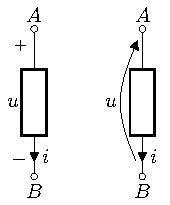
\includegraphics[width=0.5\linewidth]{figs/intro/sens_conventionnel}
	\caption[Sens conventionel d'un dip�le.]{Sens conventionnel (convention moteur) d'un dip�le. On indique le sens de la tension soit avec un signe + et un signe -, soit avec une fl�che.}
\label{fig:convetion_dipole}
\end{marginfigure}

Pour la convention moteur, le courant p�n�tre par la borne $+$ et sort par la borne $-$.
Avec cette convention, le courant sera consid�r� comme "positif' lorsque les charges positives entrent par la borne $+$ et sortent par la borne $-$ ; la d.d.p. $u$ sera consid�r�e comme "positive" lorsque le potentiel du noeud $+$ est sup�rieur � celui du noeud $-$.

L'adoption d'une convention n'est pas impos�e par des raisons physiques. L'utilisation d'une convention est n�anmoins importante : on sait que dans le cas de cette convention moteur, le produit $u(t) i(t)$ repr�sente la puissance \textbf{fournie} au dip�le � l'instant $t$.

L'analyse d'un circuit \textbf{commence toujours par l'application d'une con\-vention � chaque branche du circuit}. Mais ce n'est qu'� l'issue de l'analyse que le sens r�el des tensions et courants est d�termin� en fonction du signe que prennent les variables de mod�lisation. En utilisant la convention moteur, selon le type de dip�le consid�r� et la mani�re dont il est connect� au reste du circuit, la puissance fournie au dip�le est 
\begin{itemize}
	\item soit positive : le dip�le consomme de l'�nergie ;
	\item soit n�gative : le dip�le fournit de l'�nergie ;
	\item soit nulle.
\end{itemize} 

\subsection{Circuit passifi�}
Une notion importante, qui renviendra tr�s fr�quemment dans ce cours, est la notion de circuit \textit{ passifi�}.
On appelle \textit{\textbf{passifi�}} un circuit dont on a (par la pens�e le plus souvent) enlev� les sources ind�pendantes d'�nergie; il d�rive du circuit d'origine (complet) lorsque l'on "court-circuite" tous les g�n�rateurs de tension, c'est-�-dire lorsqu'on remplace tous ces g�n�rateurs par des conducteurs parfaits, et lorsqu'on ouvre tous les injecteurs de courant, c'est-�-dire lorsqu'on enl�ve les dip�les sources id�ales de courant.

\section{Quadrip�les}

Un quadrip�le est un (�l�ment de) circuit comportant deux acc�s (deux paires de bornes), chacun �tant caract�ris� par deux grandeurs : d.d.p. et courant. 
\begin{marginfigure}
	\centering
	\begin{circuitikz}[american voltages]% or tikzpicture
		\tikzset{quad/.style={draw, thick, minimum height=2cm, minimum width=2cm}}
		\node[quad] (A) at (0,0) {};
		\draw ($(A.north west)!.5!(A.west)$) to[short,-o, i<=$i_1$] ++(-.5,0) to[open] ++(-0.2,0) coordinate (A1)
		($(A.south west)!.5!(A.west)$) to[short,-o, i=$i_1$] ++(-.5,0) to[open] ++(-0.2,0) coordinate (A1')
		($(A.north east)!.5!(A.east)$) to[short,-o, i<=$i_2$] ++(.5,0) to[open] ++(0.2,0) coordinate (A2)
		($(A.south east)!.5!(A.east)$) to[short,-o, i=$i_2$] ++(.5,0) to[open] ++(0.2,0) coordinate (A2');
		\draw (A1) to[open, v=$u_1$] (A1');
		\draw (A2) to[open, v^=$u_2$] (A2');
	\end{circuitikz}
	\caption[Repr�sentation d'un quardip�le.]{Repr�sentation d'un quardip�le.}
	\label{fig:quadripole}
\end{marginfigure}
Plus pr�cis�ment, pour chacun des acc�s, le courant "entrant" par une de ses bornes en "sort" par l'autre. Les sens conventionnels associ�s sont indiqu�s sur la Figure~\ref{fig:quadripole}. Avec ces sens, la puissance totale fournie au quadrip�le � l'instant $t$ est exprim�e par :
$$p(t) = i_1(t) u_1(t) + i_2(t) u_2(t)$$
Notons que le quadrip�le est un cas particulier du t�trap�le; ce dernier est un circuit � quatre bornes ne constituant pas deux acc�s (Figure~\ref{fig:tetrapole}), et les courants ne sont soumis qu'� la seule contrainte impos�e par la premi�re loi de Kirchhoff (Chapitre~\ref{sec:LK}).
\begin{marginfigure}
\centering
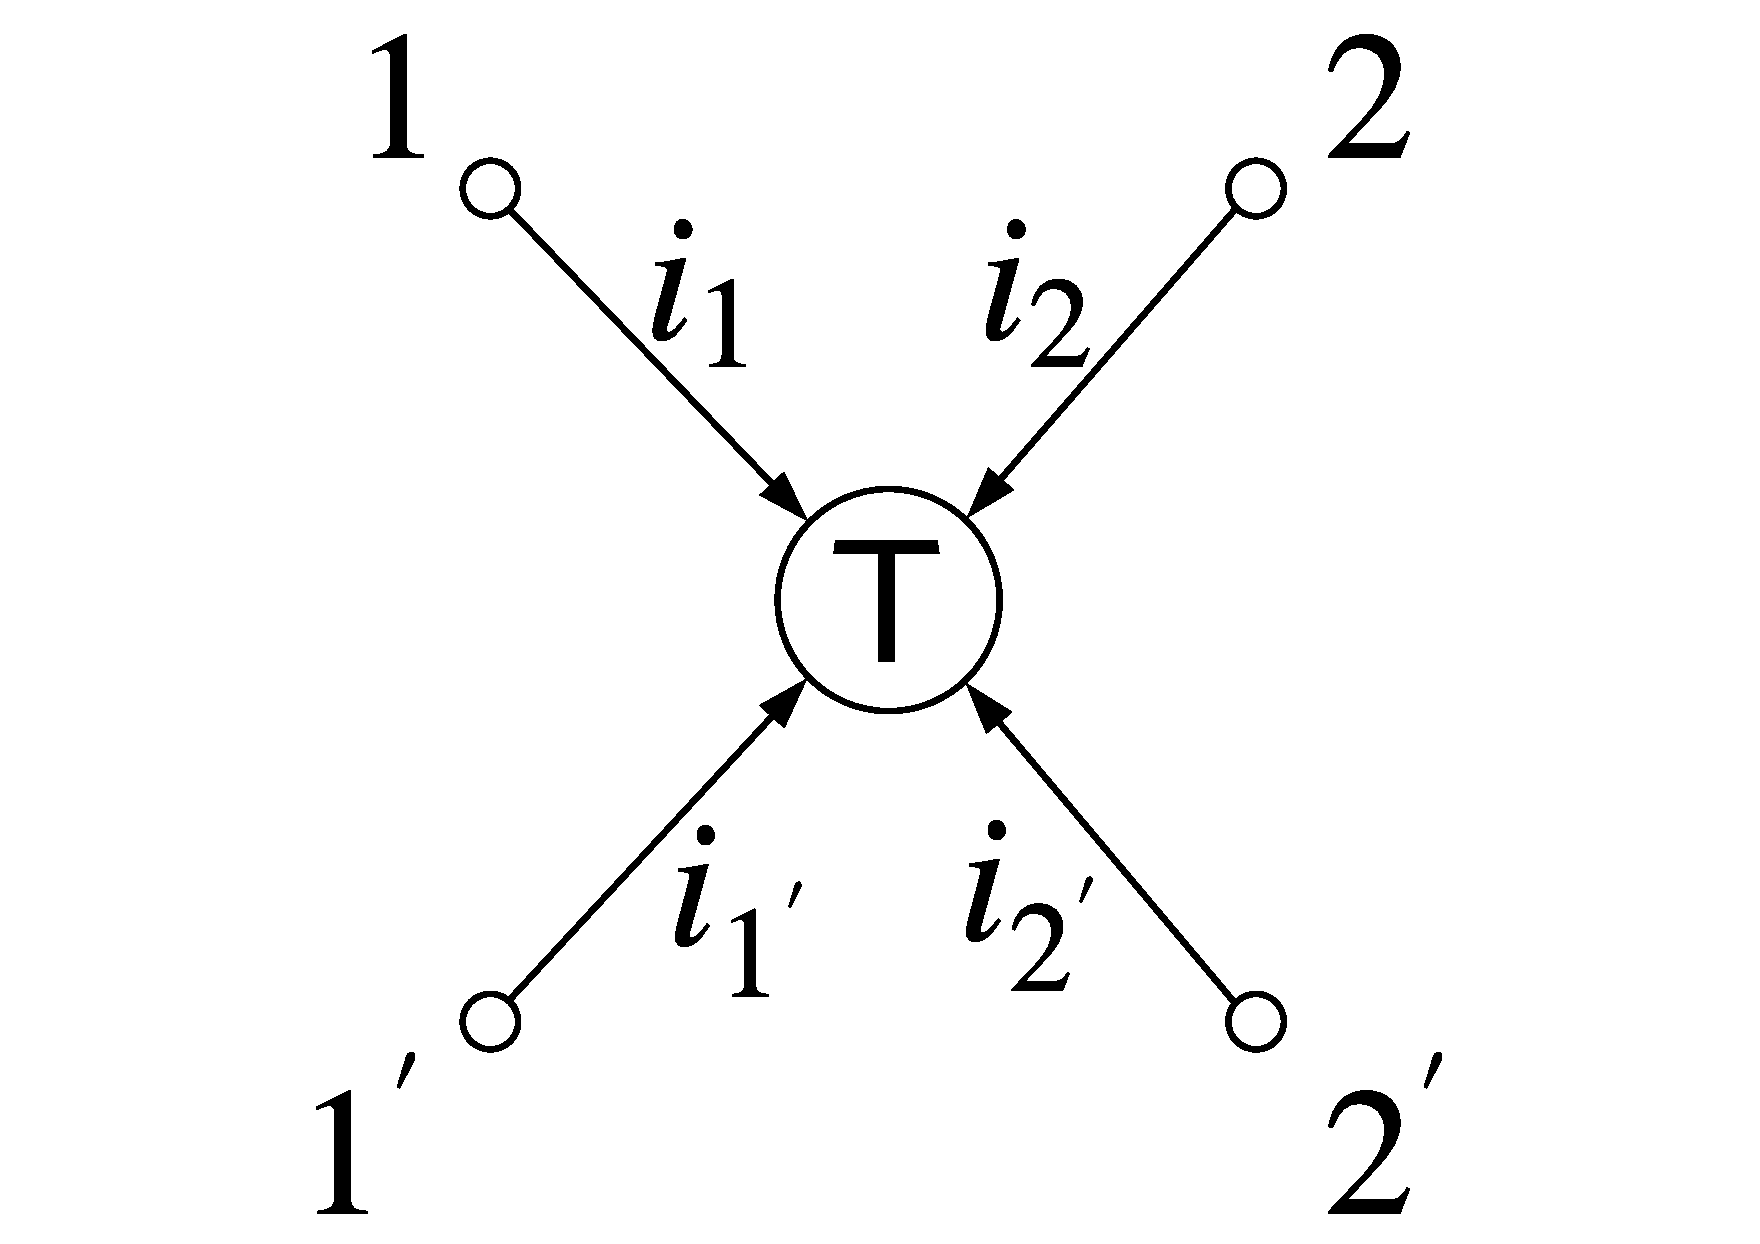
\includegraphics[width=0.7\linewidth]{figs/ch2_figs/tetrapole}
\caption{Tetrap�le.}
\label{fig:tetrapole}
\end{marginfigure}



\section{Classification des circuits}
Les propri�t�s �lectriques d'un circuit en tant que transmetteur -- ce terme �tant pris dans son sens le plus large -- d�pendent des propri�t�s de ses �l�ments, � l'exclusion des sources ind�pendantes d'�nergie. Pour identifier ces propri�t�s, nous consid�rerons donc des circuits \textit{passifi�s} et assimilerons ces derniers � des "bo�tes" dot�es d'acc�s. Leurs propri�t�s g�n�rales d�pendront de la nature des r�ponses obtenues � certains acc�s � des excitations appliqu�es � certains (les m�mes ou non) acc�s.



\subsection{Lin�arit�}
Soient $e(t)$ l'excitation appliqu�e � un syst�me\footnote{Dans ce paragraphe, nous utilisons de fa�on interchangeable les termes "circuit" et "syst�me" pour mettre l'accent sur le fait que les d�finitions sont g�n�rales et ne rev�tent pas un caract�re sp�cifiquement "�lectrique".} suppos� initialement relax�\footnote{Un syst�me est dit \textit{\textbf{initialement relax�}} lorsqu'il est d�pourvu de toute �nergie initiale emmagasin�e, c'est-�-dire de conditions initiales. Les �l�ments conventionnels introduisant des conditions initiales dans les circuits sont les inductances et les condensateurs.}, et 
$w(t)$ la r�ponse � cette excitation. On dit que le syst�me est lin�aire s'il satisfait le principe de superposition suivant lequel la r�ponse due � plusieurs excitations est �gale � la somme des r�ponses dues � chacune des excitations agissant s�par�ment\footnote{La propri�t� de superposition est �quivalente aux propri�t�s d'homog�n�it� et d'additivit� r�unies.}. Autrement dit, si :
$w_1(t)$ est la r�ponse � l'excitation $e_1(t)$ et si
$w_2(t)$ est la r�ponse � l'excitation $e_2(t)$,
alors le circuit sera lin�aire si la r�ponse � l'excitation
$k_1 e_1(t) + k_2 e_2(t)$ est $k_1 w_1(t) + k_2 w_2(t)$
avec $k1$ et $k2$ des constantes.

Cette propri�t� s'�tend bien entendu � plus de deux signaux, et ces signaux ne sont pas n�cessairement scalaires. En effet, si des  excitations sont appliqu�es � plusieurs acc�s du circuit, $e(t)$ et $w(t)$ deviennent des vecteurs.


\paragraph{Exemple.}
Un d�rivateur est un syst�me lin�aire. En effet, la d�riv�e d'une combinaison lin�aire de fonctions est �gale � cette combinaison lin�aire de leurs d�riv�es.
$$\frac{d}{dt}\left(\sum_{i=1}^n k_i e_i(t)\right) = \sum_{i=1}^n k_i \frac{d e_i(t)}{dt}$$

\subsection{Permanence ou invariance}
Si $w(t)$ est la r�ponse d'un syst�me � un signal $e(t)$ agissant � l'instant $t$, la r�ponse de ce syst�me au m�me signal mais diff�r� de $r$, $e(t-r)$, sera sa r�ponse initiale diff�r�e de $r$, c'est-�-dire $w(t - r)$.
Les syst�mes qui satisfont le principe de permanence sont dits invariants ou permanents ; sinon ils sont variants.

\paragraph{Contre-exemple.} Le syst�me d�crit par la relation $w(t) = t \frac{de(t)}{dt}$ n'est pas invariant.

\subsection{Passivit�}
Les circuits qui ne restituent jamais plus d'�nergie qu'ils n'en re�oivent sont appel�s passifs. Dans le cas contraire, ils sont appel�s actifs.
Dans le cas d'un dip�le, en d�signant par $p(t) = u(t) i(t)$ la puissance qui lui est
fournie en $t$ (attention au sens de r�f�rence associ�s) et par $W(t)$ l'�nergie qui lui est fournie jusqu'� cet instant $t$, la condition de passivit� s'exprime par :
$$ W(t) = \int_{-\infty}^t u(x) i(x) dx \ge 0.$$

Ceci doit �tre valable pour n'importe quelle d.d.p. et le courant en r�sultant pour tout $t$.
Plus g�n�ralement, la puissance instantan�e fournie � un circuit comportant plusieurs acc�s vaut :
$p(t) = \mathbf{u}^T(t)\mathbf{i}(t)$.
Ce circuit sera passif si pour tout $t$ :
$$ W(t) = \int_{-\infty}^t \mathbf{u}^T(x) \mathbf{i}(x) dx \ge 0.$$

\paragraph{Remarque.} Les circuits actifs sont d�finis � partir de l'in�galit� stricte $W(t) < 0$,
les passifs par l'in�galit� simple $W(t) \ge 0$ ; ils incluent de la sorte certains �l�ments id�alis�s, comme par exemple le transformateur id�al (Chapitre~\ref{sec:sinusoidal}) qui est effectivement passif.

\subsection{R�ciprocit�}
Un circuit (par exemple un quadrip�le, Figure~\ref{fig:quadripole}) est dit r�ciproque s'il a la propri�t� suivant laquelle la r�ponse � un de ses acc�s produite par une excitation agissant � un autre acc�s reste inchang�e lorsque l'on permute ces deux acc�s (pour autant que l'on d�finisse de fa�on consistante r�ponse et excitation). Un circuit qui ne satisfait pas cette propri�t� est dit non-r�ciproque.
Plus sp�cifiquement, la propri�t� de r�ciprocit� requiert la satisfaction d'une des trois conditions �nonc�es ci-dessous, appliqu�es � un circuit relax�, non d�g�n�r� et pourvu de deux acc�s, $11'$ et $22'$. 

%\paragraph{Propri�t�s des quadrip�les}
%Avant d'aller plus loin dans la mani�re de caract�riser les relations entre acc�s, il est int�ressant d'�noncer deux propri�t�s que peuvent avoir certains quadrip�les :
%
%\begin{enumerate}
%	\item la propri�t� de \textbf{r�ciprocit�}: un quadrip�le est r�ciproque s'il satisfait � une des trois conditions �nonc�es plus bas.
%	\item la propri�t� de \textbf{sym�trie}: on peut inverser les acc�s sans que cela ne change quoi que ce soit au comportement du syst�me englobant le quadrip�le. Les acc�s sont indiscernables. Un quadrip�le sym�trique est r�ciproque (mais l'inverse pas n�cessairement).
%\end{enumerate}

\paragraph{Amp�rem�tre et voltm�tre}
Un amp�rem�tre (Figure~\ref{fig:amperemetre}) mesure le courant.
Il se place dans la branche du courant mesur�.
Il pr�sente une r�sistance tr�s \textbf{faible}, pour ne pas influencer la mesure.
\begin{marginfigure}
\begin{center}
	\begin{circuitikz}[american voltages]% or tikzpicture
		\draw (0,0) to[ammeter] (2,0);
	\end{circuitikz}
\end{center}
\caption{Symbole de l'amp�rem�tre.}\label{fig:amperemetre}
\end{marginfigure}

Un voltm�tre (Figure~\ref{fig:voltmetre}) mesure la tension.
Il se place entre les points dont on veut mesurer la diff�rence de potentiel. Il pr�sente une r�sistance tr�s \textbf{grande}, pour ne pas influencer la mesure.
\begin{marginfigure}
\begin{center}
	\begin{circuitikz}[american voltages]% or tikzpicture
		\draw (0,0) to[voltmeter] (2,0);
	\end{circuitikz}
\end{center}
\caption{Symbole du voltm�tre.}\label{fig:voltmetre}
\end{marginfigure}


\paragraph{Condition des r�ciprocit� 1: �change de l'amp�rem�tre et de la source de tension.}
Connectons pour commencer une source de tension $v_{s1}$
� l'acc�s $11'$ ; soit $i_2^a$ le courant apparaissant � l'acc�s $22'$ court-circuit� (Figure~\ref{fig:recipro_1}).
Ensuite, connectons une source de tension $v_{s2}$ en $22'$ et mesurons le courant $i_1^b$ apparaissant aux bornes $11'$ court-circuit�es.
Le th�or�me de r�ciprocit� affirme que quelle que soit la topologie du circuit,
la valeur de ses �l�ments et la nature des g�n�rateur, on doit avoir, si $v_{s1}(t)=v_{s2}(t)$ $\forall t$,
\[i_1^b(t)=i_2^a(t) \,\, \forall t.\]
\begin{figure}[h]
\begin{center}
	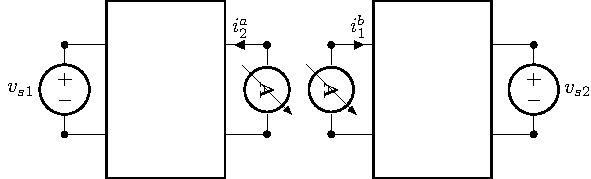
\includegraphics[width=0.98\linewidth]{figs/intro/QP_AvsV}
\end{center}
\caption{\'Echange de l'amp�rem�tre et de la source de tension.}\label{fig:recipro_1}
\end{figure}

\paragraph{Condition des r�ciprocit� 2: �change du voltm�tre et de la source de courant.}
Connectons pour commencer une source de courant $i_{s1}$ �
l'acc�s $11'$ et mesurons la d.d.p. $u_2^a$ apparaissant en $22'$ (Figure~\ref{fig:recipro_2}). Ensuite,
connectons une source de courant $i_{s2}$ en $22'$ et mesurons la d.d.p. $u_1^b$ apparaissant en
$11'$. Le th�or�me de r�ciprocit� affirme que quelle que soit la topologie
du circuit, la valeur de ses �l�ments et la nature des injecteurs de courant, on doit
avoir, si $i_{s1}(t)=i_{s2}(t) \,\, \forall t$, 
\[u_1^b(t)=u_2^a(t) \,\, \forall t\]
\begin{figure}[h]
	\centering
	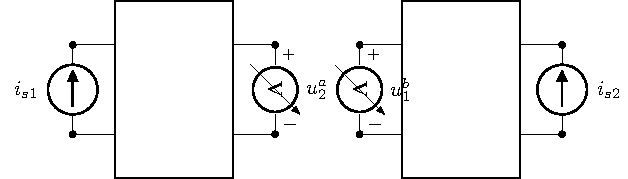
\includegraphics[width=0.98\linewidth]{figs/intro/QP_VvsJ}
\caption{\'Echange du voltm�tre et de la source de courant.}\label{fig:recipro_2}
\end{figure}



\paragraph{Condition des r�ciprocit� 3}

Connectons une source de courant $i_{s1}$ � l'acc�s $11'$ et mesurons
la valeur du courant parcourant l'acc�s $22'$ court-circuit� (Figure\ref{fig:recipro_3}). Ensuite, connectons une source de tension $u_{s2}$ en $22'$ et mesurons la d.d.p. aux bornes $11'$. Le th�or�me de r�ciprocit� affirme que, quelle que soit la topologie du circuit,
la valeur de ses �l�ments et la nature des sources, on doit avoir
pour autant que $i_{s1}(t)=u_{s2}(t) \,\, \forall t$,
\[u_1^b(t)=i_2^a(t) \,\, \forall t\]
\begin{figure}[h]
	\centering
	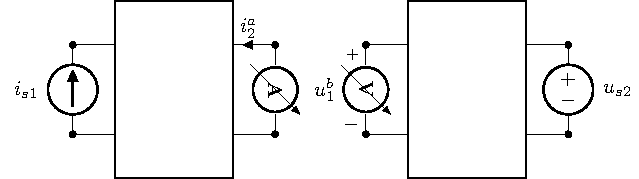
\includegraphics[width=0.98\linewidth]{figs/intro/QP_recipro_3}
\caption{Troisi�me condition de r�ciprocit�.}\label{fig:recipro_3}
\end{figure}


\section{Organisation du cours}

Dans la suite du cours nous introduirons d'abord les lois fondamentales (Ohm, Kirchhoff) et les composants de base des circuits (r�sistance, condensateur, bobine, sources d'�nergie). Nous commencerons par un fonctionnement en courant continu, puis analyserons les cons�quences de changement brutaux de fonctionnement du syst�me, les r�gimes transitoires, et enfin nous verrons comment fonctionnent les circuits � courant alternatif, essentiellement utilis�s pour le transport et la distribution de l'�lectricit�. 
Les chapitres suivant se focaliseront sur sur les filtres et les diff�rentes utilisations de l'amplificateur op�rationnel.
Ensuite nous �noncerons les th�or�mes fondamentaux, dans le but de pouvoir simplifier des circuits complexes (Th�venin et Norton). La derni�re partie du cours �tudiera les m�thodes g�n�rales d'analyse qui permettent de syst�matiser l'�tude des circuits, d'en obtenir des �quivalents � plusieurs acc�s, et sont � la base des m�thodes d'analyse num�rique modernes.

Deux approches transversales seront utilis�es pour illustrer et enrichir les concepts �tudi�s tout au long de ce texte.

\subsection{R�alisations pratiques} 
\label{sec:pratique}
Des exemples de r�alisations pratiques de circuits relativement complexes seront pr�sent�es et analys�s au fil des chapitres. 

\paragraph{Radio AM.}
C'est en r�alit� un poste de radio appel� r�cepteur � cristal, o� l'on a ajout� des amplificateurs. Le but d'un tel circuit est de produire un son gr�ce � un signal radio capt� de l'ext�rieur, typiquement en provenance d'une source d'�mission d'un groupe de m�dias. Il existe encore quelques �metteurs pour ce type de radio, mais cette technologie a depuis longtemps �t� remplac�e par d'autres m�thodes analogiques d'abord, et maintenant num�riques (par exemple le \textit{Digital Audio Broadcasting}). Elle pr�sente cependant l'avantage d'�tre simple et illustre une grande partie des concepts de ce cours.  Le circuit �lectrique correspondant est sch�matis� � la Figure~\ref{fig:radio}.\mytodo{meilleur sch�ma ? Photo ?}
\begin{figure}[htb]
\centering
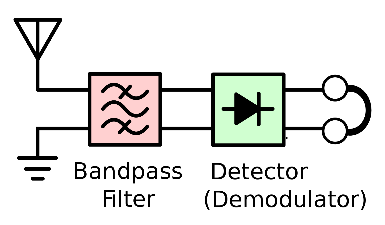
\includegraphics[width=0.45\textwidth]{figs/RadioAM/radio1}  
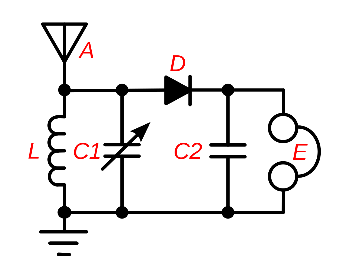
\includegraphics[width=0.45\textwidth]{figs/RadioAM/radio2}
\caption{Sch�ma d'une radio cristal. Le signal est capt� par une antenne, filtr�, d�modul� pour finalement �tre �cout� via des �couteurs.}
\label{fig:radio}
\end{figure}
La radio cristal est une radio AM (\textit{amplitude modulation}), ce qui signifie qu'elle re�oit des signaux modul�s en amplitude (Figure~\ref{fig:mod1}). La modulation peut se voir comme la mani�re de "coder" un signal sonore. La modulation d'amplitude d�signe la variation en amplitude d'un signal de fr�quence �lev�e (signal porteur, Figure~\ref{fig:mod2}) en fonction d'un signal de plus basse fr�quence (signal modulant, Figure~\ref{fig:mod3}). Ce dernier contient l'information audio � transmettre. 

\begin{figure}[h!]
	\centering
	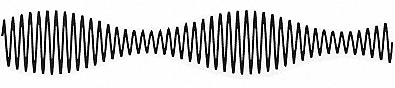
\includegraphics[width=7cm]{figs/RadioAM/mod3}
	\caption{signal modul�}
	\label{fig:mod1}
\end{figure}
\begin{figure}[h!]
   	\centering
   	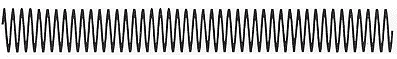
\includegraphics[width=7cm]{figs/RadioAM/mod1}
   	\caption{signal porteur (fr�quence radio)}
   	\label{fig:mod2}
\end{figure}
\begin{figure}[h!]
   	\centering
   	
\includegraphics[width=7cm]{figs/RadioAM/mod2}
   	\caption{signal modulant (fr�quence audio)}
   	\label{fig:mod3}
\end{figure}

Les fr�quences audibles sont comprises entre 16Hz et 16kHz (signal modulant BF). Typiquement, les fr�quences AM s'�tendent de 500 kHz � 1600 kHz (signal porteur basse fr�quence). Cependant, l'antenne radio capte tout ce qu'elle peut capter dans l'environnement, y compris du bruit. Pour capter uniquement la bande de fr�quences d�sir�e et se d�barrasser du reste, il faut un filtre \textit{passe-bande} (cf. Chapitre~\ref{cha:filtres}).

Un autre �l�ment crucial du circuit est le d�tecteur � cristal (d'o� le nom radio "cristal")\footnote{\'Egalement connu sous les noms de poste � gal�ne, ou poste � diode.}. Il s'agit d'une diode (Section~\ref{sec:diode}) qui va contribuer � la d�modulation du signal radio pour en extraire le signal audio. Ce type de r�cepteur a �t� introduit au d�but du vingti�me si�cle et est le moyen le plus simple de construire une radio.

Dans un r�cepteur de base le son peut finalement �tre entendu gr�ce � des �couteurs. Ceux-ci ne fonctionnent que gr�ce � l'�nergie de l'onde radio elle-m�me, et doivent donc �tre tr�s sensibles. Dans notre circuit, nous avons donc remplac� les �couteurs par un haut-parleur. En cons�quence, il a �galement fallu ajouter des amplificateurs op�rationnels (Chapitre~\ref{cha:AO}) pour amplifier le signal. Ce sont des composants actifs qui ont donc besoin d'une alimentation.

%\mytodo{Un circuit complexe dont on veut identifier les param�tres pour r�aliser un �quivalent simplifi�, comme par exemple une batterie compos�e de plusieurs cellules}


\subsection{M�thodes num�riques}
Des exemples en Python permettent d'automatiser et passer d'analyses de petits syst�mes � des syst�mes plus complexes, inaccessibles par calcul manuel, comme par exemple :
\begin{itemize}
	\item associer des imp�dances en s�rie, en parall�le
	\item convertir une association en �toile en une association en triangle
	\item manipuler les nombres complexes, calculer des puissances 
	\item manipuler des graphes
	\item r�soudre des syst�mes d'�quations diff�rentielles pour analyser les r�gimes transitoires
	\item impl�menter les m�thodes g�n�rales d'analyse.
\end{itemize}

Le code source des exemples est disponible � l'adresse
\begin{center}
	\small
\url{https://github.com/bcornelusse/ELEC0053-circuits-electriques}.
\end{center}

\section{Liens avec d'autres cours}
Ce cours ouvre la voie � une s�rie importante d'autres cours tels que les cours sur la conception des capteurs, sur les syst�mes de mesure, l'�lectronique analogique, l'�lectronique de puissance, l'analyse et le contr�le de grands syst�mes �lectriques, les micro-syst�mes, l'�lectro-acoustique, les micro-r�seaux, pour ne citer qu'eux.
% !TeX encoding = ISO-8859-1
% !TeX spellcheck = fr_FR
% !TeX root = syllabus_ELEC0053.tex


\chapter{Lois fondamentales et composants fondamentaux}
\label{fig:lois}

\textit{Ce chapitre �nonce les lois fondamentales et les mod�les de composants qui permettent l'�tude de circuits localis�s.
Avant d'�noncer ces lois et mod�les, un bref rappel de th�orie des graphes s'impose. Il sera utile pour l'ensemble du cours.
}
\section{Rappel de th�orie des graphes}
La th�orie des graphes est une discipline de l'alg�bre lin�aire qui re�oit de nos jours de nombreuses applications. En th�orie des circuits �lectriques, notamment, elle rend des services pr�cieux. Ainsi, dans le domaine de l'analyse, elle procure un �ventail de m�thodes syst�matiques, se distinguant par la nature des variables et par le nombre d'�quations y aff�rant. L'existence de telles m�thodes est essentielle surtout quand il
s'agit de grands syst�mes -- et les circuits �lectriques constituent souvent de tr�s grands syst�mes ; pour ne citer qu'un exemple, les r�seaux de transport d'�nergie �lectrique � haute tension comportent couramment des centaines, voire des milliers de noeuds et bien davantage de branches et de mailles. Une syst�matique rigoureuse est alors indispensable pour identifier et traiter les variables �lectriques appropri�es. Ceci explique \textit{a posteriori} le fait que la th�orie des graphes fut originairement �bauch�e par le fondateur m�me de la th�orie des circuits\footnote{G. KIRCHHOFF, "�ber die Aufl�sing der Gleichungen, auf welche man bei der Untersuchungen der Linearen Verteilung Galvanischer Str�me gef�hrt wird". Poggendorf Ann. Physik, 72, 1847.} pour les besoins de ceux-ci.

\subsection{D�finitions g�n�rales}
\paragraph{Branche.}\footnote{"Branch" ou "edge"en anglais.} C'est un segment de ligne dont les deux extr�mit�s sont distinctes.

\paragraph{Noeud ou sommet.}\footnote{"Node" ou "vertex" en anglais.} C'est l'extr�mit� d'une branche.
En fait, on admettra �galement qu'un noeud peut �tre un point isol�.

\paragraph{Graphe.} Un graphe $G$ (Figure~\ref{fig:G}) est un ensemble de noeuds dont
certains sont reli�s par des branches. On d�signe par $n$ le nombre
de noeuds et par $b$ le nombre de branches.
\begin{marginfigure}[-1cm]
	\centering
	\begin{tikzpicture}
	\node[circle, draw, fill=black, scale = 0.4] (A) at (0,0) {};
	\node[circle, draw, fill=black, scale = 0.4] (B) at (2,0) {};
	\node[circle, draw, fill=black, scale = 0.4] (A2) at (0,-1) {};
	\node[circle, draw, fill=black, scale = 0.4] (B2) at (3,-1) {};
	\node[circle, draw, fill=black, scale = 0.4] (A3) at (-1,-.5) {};
	\node[circle, draw, fill=black, scale = 0.4] (B3) at (2,-1.5) {};
	\draw[black] (A) -- (B) -- (A2) -- (B3) ;
	\end{tikzpicture}
	\caption{Un graphe $G$ avec $n=6$ et $b=4$.}
	\label{fig:G}
\end{marginfigure}


\paragraph{Branche orient�e.} C'est une branche poss�dant une orientation fix�e par
l'ordre des noeuds. Cette orientation est indiqu�e par une fl�che pointant vers le second noeud de la paire orient�e. Par exemple, la Figure~\ref{fig:G1}  d�signe la branche orient�e $ab$.
Il est quelquefois utile de consid�rer seul le segment de ligne (branche sans ses extr�mit�s), on parle alors d'\textbf{arc} si la branche � laquelle appartient le segment de ligne est orient�e et d'\textbf{ar�te} si cette branche n'est pas orient�e.
\begin{marginfigure}[-1.5cm]
	\centering
	\begin{tikzpicture}
	\node[circle, draw, fill=black, scale = 0.4] (A) at (0,0) {};
	\node[circle, draw, fill=black, scale = 0.4] (B) at (2,0) {};
	\draw[arrows=-triangle 45,black] (A) node[above] {$a$} -- (B) node[above] {$b$} ;
	\node[circle, scale = 0.4] (A2) at (0,-0.5) {};
	\node[circle, scale = 0.4] (B2) at (2,-.5) {};
	\draw[arrows=-triangle 45,black] (A2) node[above] {$a$} -- (B2) node[above] {$b$} ;
	\node[circle, scale = 0.4] (A3) at (0,-1) {};
	\node[circle, scale = 0.4] (B3) at (2,-1) {};
	\draw[black] (A3)  node[above] {$a$} -- (B3) node[above] {$b$} ;
	\end{tikzpicture}
	\caption{Branche orient�e entre les noeuds $a$ et $b$, arc et ar�te.}
	\label{fig:G1}
\end{marginfigure}

\paragraph{Graphe orient�.} Un graphe est orient� lorsque toutes ses branches le sont. 
Dans la th�orie des circuits, seuls les graphes orient�s nous int�ressent, m�me si certaines d�finitions de ce chapitre
s'appliquent indistinctement aux graphes orient�s ou non.
\begin{marginfigure}[-1cm]
\centering
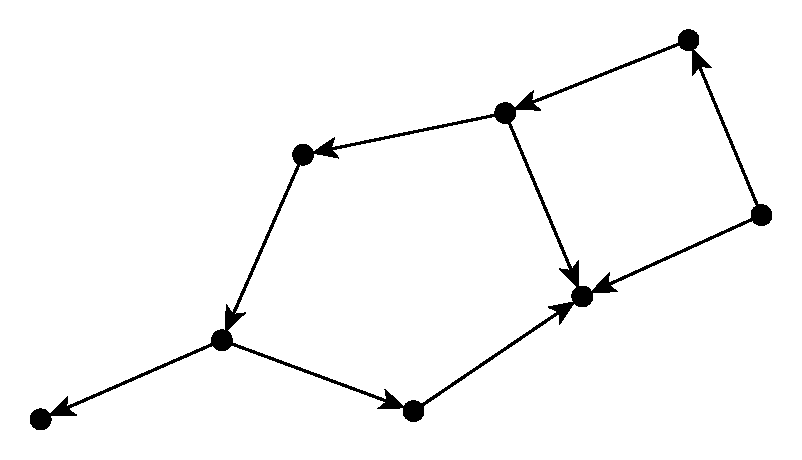
\includegraphics[width=0.9\linewidth]{figs/graphes/DG}
\caption{Graphe orient�.}
\label{fig:DG}
\end{marginfigure}


\paragraph{Sous-graphe.} Un sous-graphe d'un graphe est un sous-ensemble des branches
du graphe ; c'est lui-m�me un graphe. Il est dit "propre" s'il ne contient pas toutes les
branches du graphe dont il est issu.
\begin{marginfigure}[1cm]
	\centering
	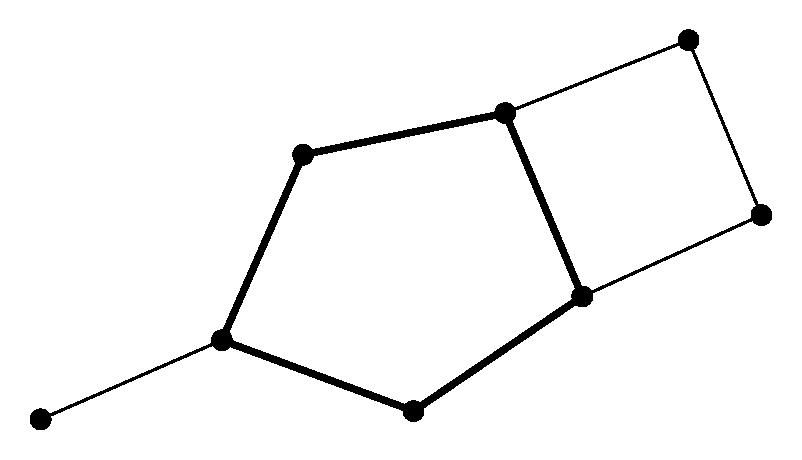
\includegraphics[width=0.9\linewidth]{figs/graphes/subgraph}
	\caption{Sous graphe (ar�tes en trait �pais et noeuds incidents.)}
	\label{fig:sous_graphe}
\end{marginfigure}


\paragraph{Incidence.} On dit qu'une branche $b$ est incidente � un noeud $n$ si $n$ est une
extr�mit� de $b$.

\paragraph{Isomorphisme.} On dit que les graphes $G$ et $G'$ sont isomorphes s'il existe
une correspondance biunivoque entre d'une part les noeuds, d'autre part les branches
de $G$ et de $G'$ qui pr�serve les relations d'incidence.
\begin{marginfigure}
	\centering
	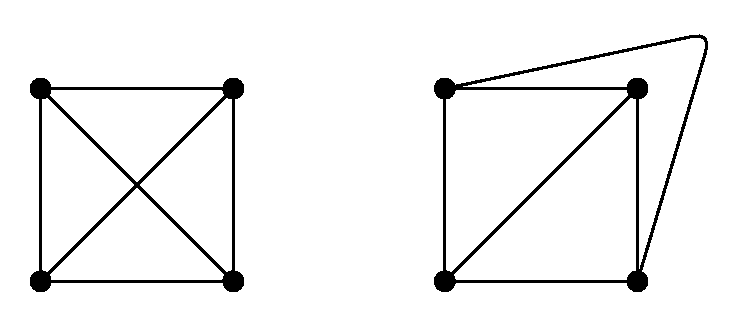
\includegraphics[width=0.9\linewidth]{figs/graphes/planar}
	\caption{Deux graphes isomorphes.}
	\label{fig:isomo}
\end{marginfigure}

\paragraph{Parcours ou chemin.}\footnote{Path en anglais.} C'est un sous-graphe d'un graphe compos�
d'une suite ordonn�e de branches dont chacune a un noeud commun avec la branche pr�c�dente et l'autre noeud commun avec la branche suivante et o� chaque noeud n'appara�t qu'une fois au plus.
\begin{marginfigure}[1cm]
	\centering
	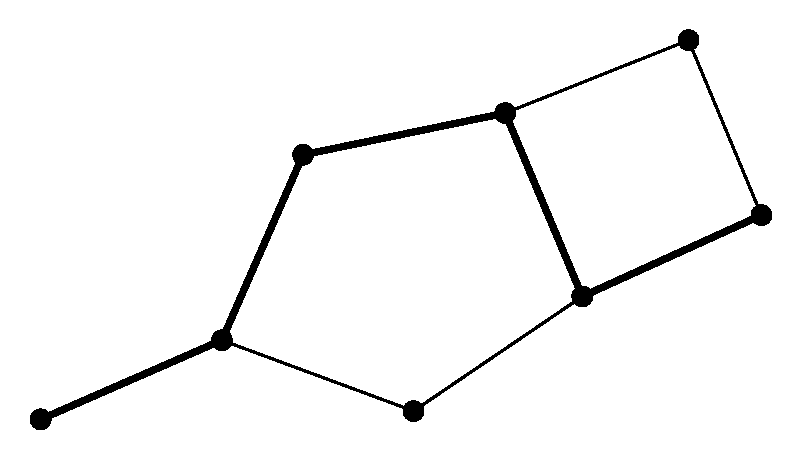
\includegraphics[width=0.9\linewidth]{figs/graphes/chemin}
	\caption{Chemin (trait �pais).}
	\label{fig:chemin}
\end{marginfigure}

\paragraph{Noeuds initial et final.} Le noeud de la premi�re branche d'un parcours qui n'appartient pas � la seconde branche est le noeud initial ; le noeud de la derni�re branche du parcours qui n'appartient pas � l'avant-derni�re branche est le noeud final. Les noeuds initial et final forment les extr�mit�s d'un chemin.

\paragraph{Degr� d'un noeud.} C'est le nombre de branches incidentes � ce noeud. Dans le graphe de la Figure~\ref{fig:chemin}, il y a $1$ noeud de degr� $1$, $4$ noeuds de degr� $2$ et $3$ noeuds de degr� $3$.

\paragraph{Graphe connexe.} Un graphe est dit connexe (ou simplement connexe) s'il existe toujours un parcours entre deux quelconques de ses noeuds. Intuitivement un graphe est connexe s'il est d'une pi�ce. Sinon, il est appel� non-connexe ou multiplement connexe.
Dans ce dernier cas, il est constitu� d'un certain nombre $p$ de parties connexes ; on dit alors que le graphe est $p-$connexe.
Le graphe de la Figure~\ref{fig:G} est 3-connexe. 

\paragraph{Rang d'un graphe.} C'est par d�finition la diff�rence $n-p$ , o� $n$ est le nombre
total de noeuds du graphe.

\paragraph{Maille.}\footnote{Loop en anglais.} Une maille d'un graphe est un sous-graphe connexe dont tous
les noeuds sont de degr� $2$.
\begin{figure}[htb]
\centering
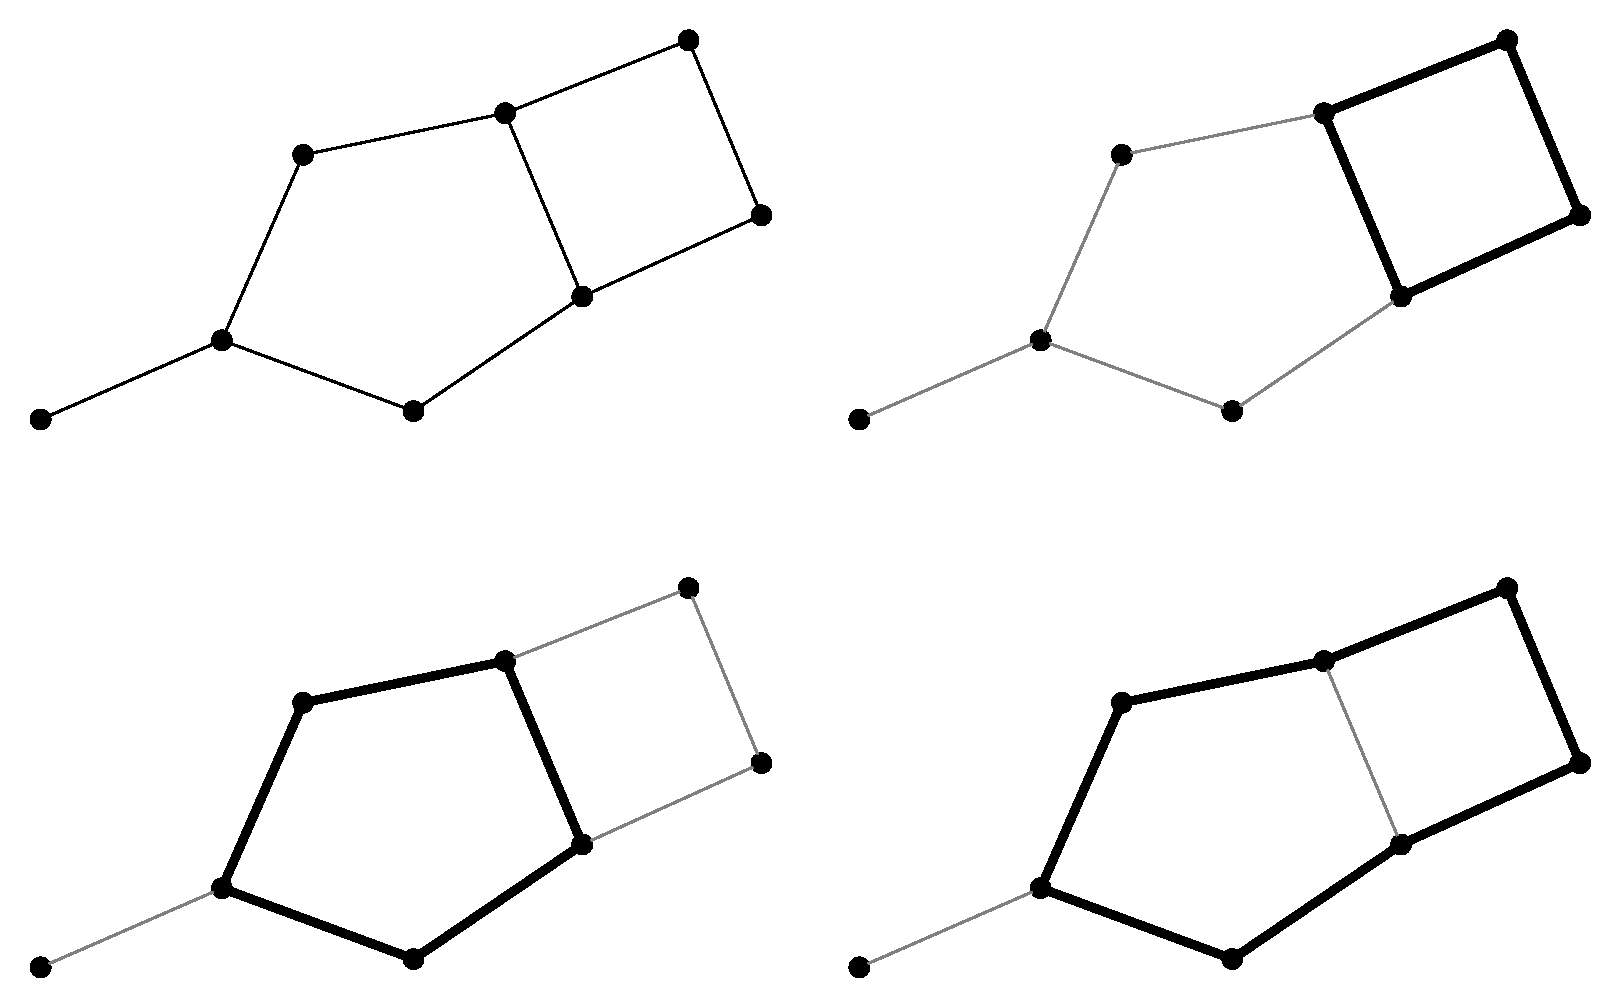
\includegraphics[width=0.8\linewidth]{figs/graphes/mailles}
\caption{Un graphes et trois mailles.}
\label{fig:mailles}
\end{figure}

\paragraph{Coupe.}\footnote{Cut-set en anglais.} Une coupe d'un graphe est un ensemble de branches dont la suppression augmente d'une unit� le nombre de connexit� et tel que la suppression de toutes ces branches moins une n'alt�re pas le degr� de connexit� du graphe. Autrement dit, une coupe est un ensemble minimal de branches dont la suppression augmente d'une
unit� la connexit� du graphe.

En particulier, on appelle \textit{coupe nodale} l'ensemble de branches incidentes � un noeud. 

Ainsi, une coupe divise les noeuds d'un graphe connexe en deux groupes. Chaque branche de la coupe a une des extr�mit�s confondue avec un noeud appartenant � l'un des groupes, l'autre de ses extr�mit�s �tant un noeud de l'autre.

\paragraph{Arbre (de recouvrement).}\footnote{Spanning-tree en anglais.} Sous-graphe connexe qui contient tous les noeuds du graphe initial et qui ne comporte aucune maille.
Nombre de branches de l'arbre pour r�seau connexe : $n-1$

\paragraph{Maillon.} Les branches restantes non incluses dans l'arbre de recouvrement.
Nombre de maillons : $b-(n-1)$

\paragraph{Maille fondamentale.} Pour un arbre donn�, c'est une maille form�e � partir d'un seul maillon et de branches de l'arbre.
\begin{figure}[htb]
\centering
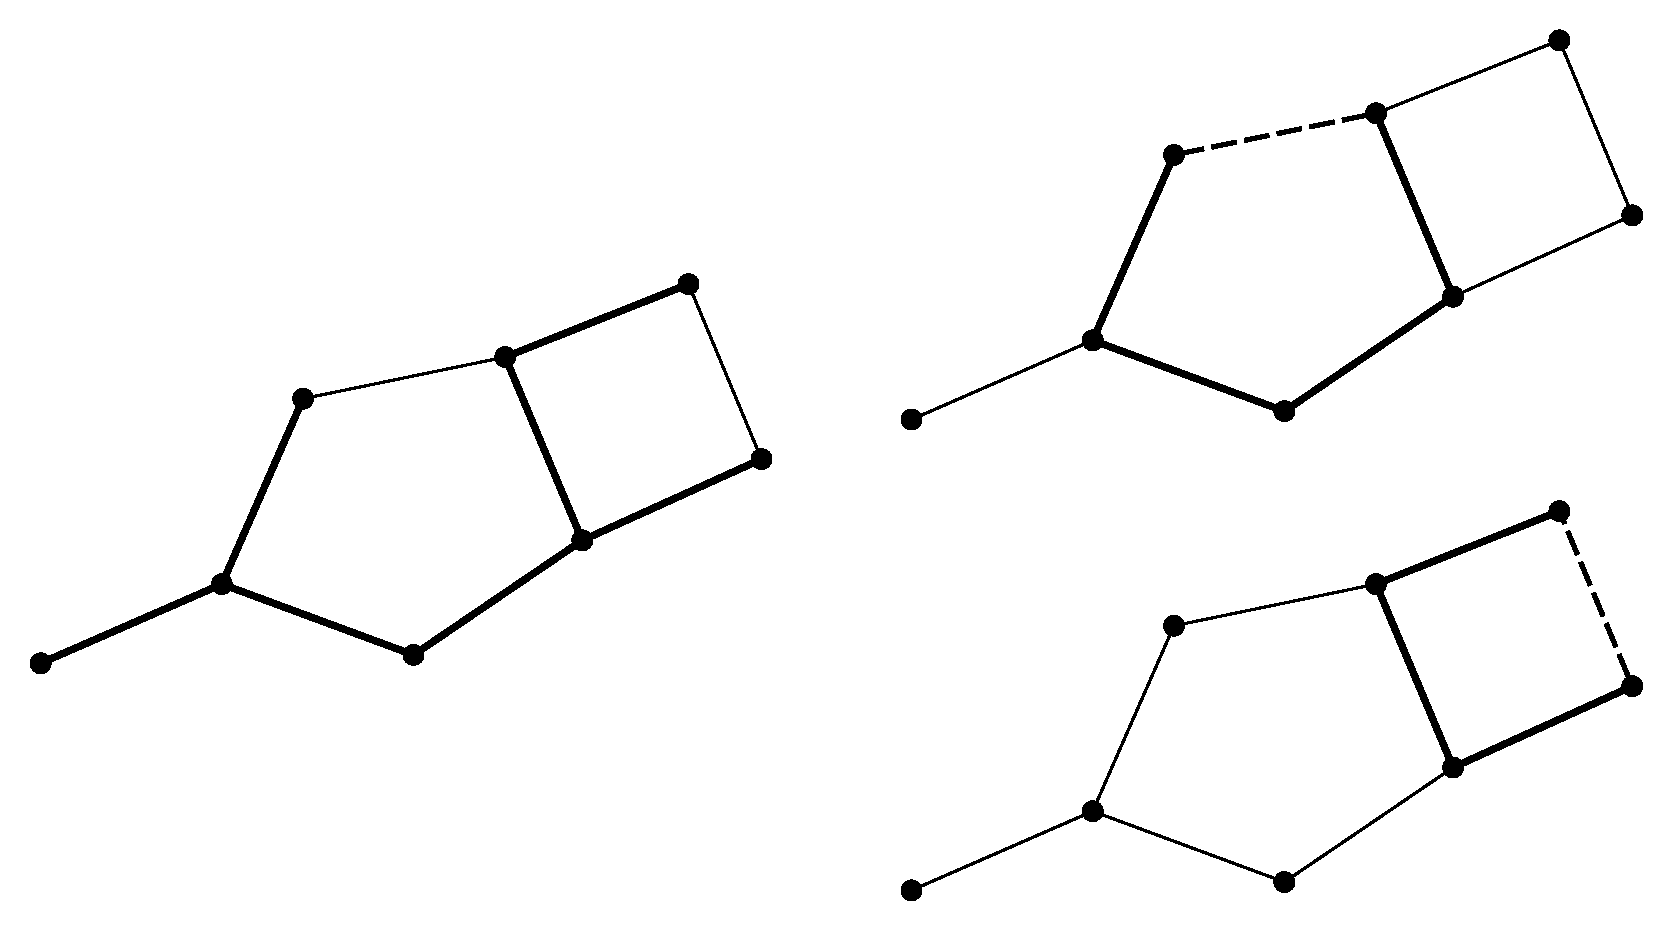
\includegraphics[width=0.8\linewidth]{figs/graphes/mailles_fondamentales}
\caption{Gauche : Un graphe et un arbre de recouvrement (en trait �pais). Droite : Maillons (trait interrompu) et mailles fondamentales correspondantes.}
\label{fig:mailles_fondamentales}
\end{figure}


\subsection{Circuit et graphe}

Toutes ces d�finitions sont utiles car on associe � un circuit �lectrique un graphe orient� (Figure~\ref{fig:circuit_et_graphe}), dont l'orientation des branches est donn�e par le sens du courant. Un graphe "math�matique" est en quelques sorte la repr�sentation la plus simple possible de la topologie d'un circuit. On se limite aux seuls graphes connexes, et on d�finit : 
\begin{itemize}
	\item $n$ : le nombre de noeuds du graphe ou du circuit
	\item $b$ : le nombre de branches
	\item le nombre de branches d'un arbre : $N=n-1$
	\item le nombre de mailles fondamentales : $M=b-(n-1)$
\end{itemize}
\begin{figure}[htb]
\centering
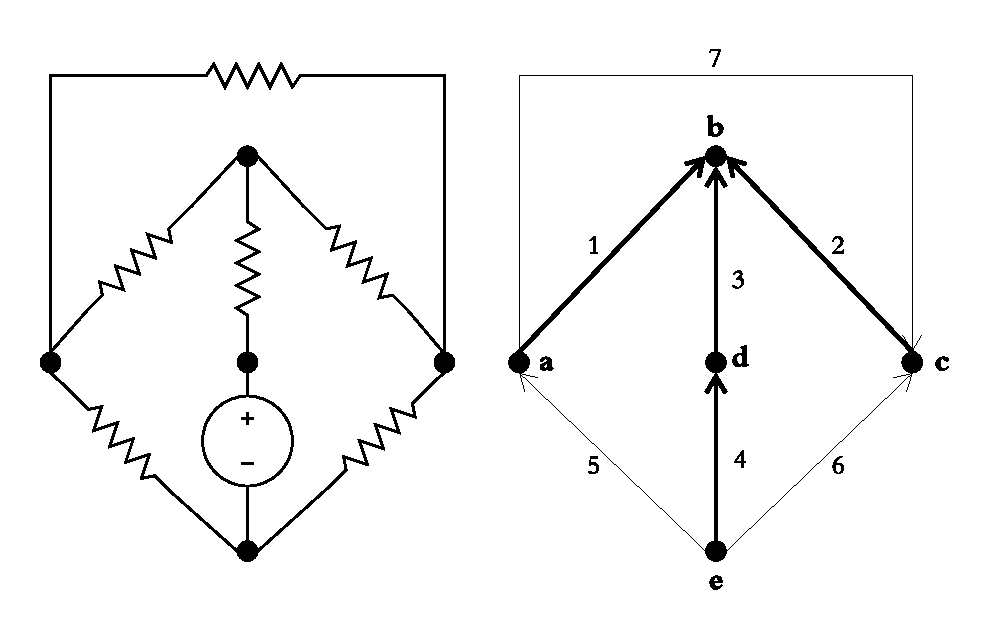
\includegraphics[width=0.9\linewidth]{figs/graphes/circuit_et_graphe}
\caption{Un circuit et sa repr�sentation sous forme de graphe. Il contient $n=5$ noeuds, $b=7$ branches, et $M=3$ maillons. Un arbre est constitu� par les branches $1$, $2$, $3$ et $4$.} 
\label{fig:circuit_et_graphe}
\end{figure}


\section{D�finitions}
\paragraph{\'Etat.} L'\textit{�tat �lectrique}, ou plus simplement \textit{�tat}, d'un r�seau donn� par sa topologie et ses �l�ments est l'ensemble des valeurs que pren\-nent les courants et les tensions de branches, $({\bf i}_B(t)$ et ${\bf u}_B(t))$, � un instant donn�. L'�tat �lectrique d�pend �videmment des signaux d�livr�s par les sources ind�pendantes d'�nergie (excitations).

\paragraph{Solution.} Dans un sens large, une \textit{solution} est l'ensemble des valeurs des courants et tensions de branches ; dans un sens plus restreint, elle est constitu�e des valeurs que prennent les variables lin�airement ind�pendantes, � partir desquelles l'�tat �lectrique complet peut �tre d�termin�.

\paragraph{R�ponse.} Une \textit{r�ponse} d'un r�seau � un ensemble d'excitations est constitu�e d'une partie de la solution du r�seau relative � ces excitations.

\section{Lois de Kirchhoff}
\label{sec:LK}

Nous pr�sentons maintenant les lois fondamentales qui permettent de d�duire l'�tat d'un circuit.

La th�orie des circuits localis�s postule la localisation des champs exclusivement � l'int�rieur de leurs �l�ments. Ceci se traduit par les deux hypoth�ses :
\begin{enumerate}
\item pas d'accumulation de charges aux noeuds d'un circuit pas plus que dans les conducteurs connectant ses �l�ments ;
\item  l'int�grale de ligne de l'intensit� du champ �lectrique total le long d'un contour associ� � une paire de noeuds d�pend exclusivement de ces noeuds: 
$$\int_1^2 
\overrightarrow{E}. \overrightarrow{d\ell}$$ est ind�pendant du chemin suivi entre $1$ et $2$.
\end{enumerate}

Les lois de Kirchhoff reposent sur ces hypoth�ses. Elles sont ind�pendantes de la nature des �l�ments constituant le circuit et expriment les contraintes impos�es par la mani�re dont les �l�ments sont interconnect�s, i.e. par la {\em topologie} ou le graphe du circuit.

\subsection{Premi�re loi de Kirchhoff (PLK) ou loi des noeuds}
La PLK exprime le principe de la conservation de la charge dans le cadre des
circuits localis�s.
La Table~\ref{tab:PLK} �nonce la premi�re loi, illustr�e � la Figure~\ref{fig:PLK}.
\begin{table}[h]
\caption{Premi�re loi de Kirchhoff.\label{tab:PLK}}
\begin{boxedminipage}{\textwidth}
	{Pour tout circuit localis�, la somme alg�brique des 
		courants de toutes les branches partant d'un noeud est nulle �
		tout instant.}
\begin{equation}
\sum_{b\in \cal{N}}i_b(t)=0 \label{eq:PLK}
\end{equation}
\end{boxedminipage}
\end{table}
\begin{marginfigure}
	\centering
	\begin{tikzpicture}[y=-1cm]
\filldraw[black] (3.02222,2.81111) circle (0.07cm);
\draw[black] (2,1.6) -- (3,2.8);
\draw[black] (3.01111,2.8) -- (2.2,4.02222);
\draw[black] (3.01111,2.8) -- (3.48889,3.73333);
\draw[black] (3.02222,2.81111) -- (4.3,2.13333);
\draw[black] (3.02222,2.81111) -- (3.35556,1.68889);
\draw[arrows=-triangle 45,black] (2.52222,2.2) -- (2.25556,1.87778);
\draw[arrows=-triangle 45,black] (3.23333,2.07778) -- (3.33333,1.77778);
\draw[arrows=-triangle 45,black] (3.73333,2.41111) -- (4.11111,2.25556);
\draw[arrows=-triangle 45,black] (3.35556,3.46667) -- (3.47778,3.7);
\draw[arrows=-triangle 45,black] (2.46667,3.61111) -- (2.28889,3.91111);
\path (2.32222,1.86667) node[text=black,anchor=base west] {$i_b$};
\end{tikzpicture}%

	\caption{Premi�re loi de Kirchhoff.\label{fig:PLK}}
\end{marginfigure}

\paragraph{D�monstration.}
Pour d�montrer cette premi�re loi, appliquons � l'�quation de Maxwell
$$\vec{\nabla} \times \overrightarrow{H}  = 
\overrightarrow{J} + \frac{\partial \overrightarrow{D}}{\partial t}$$
l'identit�
$$\vec{\nabla}.\left(\vec{\nabla} \times \overrightarrow{X}\right) = 0.$$
Ainsi
\begin{align*}\vec{\nabla}.\left(\overrightarrow{J} + \frac{\partial \overrightarrow{D}}{\partial t}\right) &= 0 \\
& = \vec{\nabla}.\overrightarrow{J} + \frac{\partial }{\partial t}\vec{\nabla}.\overrightarrow{D}\\
&= \vec{\nabla}.\overrightarrow{J} + \frac{\partial \rho}{\partial t}
\end{align*}
Int�grant sur une surface ferm�e $S$ (Figure~\ref{fig:int_S}) :
\begin{align*}
\int_S \overrightarrow{J}.\overrightarrow{dS} 
&= \int_V \vec{\nabla}.\overrightarrow{J} dV \\
&= -\int_V \frac{\partial \rho}{\partial t} dV \\ 
&= \sum_{b\in \cal{N}}i_b(t) 
\end{align*}
\begin{marginfigure}
	\centering
	\begin{tikzpicture}[y=-1cm]
\sf
\draw[dashed,black] (3.01111,2.81111) circle (0.66444cm);
\filldraw[black] (3.02222,2.81111) circle (0.06667cm);
\draw[black] (2,1.6) -- (3,2.8);
\draw[black] (3.01111,2.8) -- (2.2,4.02222);
\draw[black] (3.01111,2.8) -- (3.48889,3.73333);
\draw[black] (3.02222,2.81111) -- (4.3,2.13333);
\draw[black] (3.02222,2.81111) -- (3.35556,1.68889);
\draw[arrows=-triangle 45,black] (2.52222,2.2) -- (2.25556,1.87778);
\draw[arrows=-triangle 45,black] (3.23333,2.07778) -- (3.33333,1.77778);
\draw[arrows=-triangle 45,black] (3.73333,2.41111) -- (4.11111,2.25556);
\draw[arrows=-triangle 45,black] (3.35556,3.46667) -- (3.47778,3.7);
\draw[arrows=-triangle 45,black] (2.46667,3.61111) -- (2.28889,3.91111);
\path (2.32222,1.86667) node[text=black,anchor=base west] {$i_b$};
\path (2.24444,2.97778) node[text=black,anchor=base east] {$S$};

\end{tikzpicture}%

%% Configure (x)emacs for this file ...
%% Local Variables:
%% mode: latex
%% End:
	\caption{Int�grale sur une surface ferm�e $S$.} \label{fig:int_S}
\end{marginfigure}
Car si l'on est dans le cas d'un circuit � courant continu alors $\frac{d\rho}{dt}=0$, et sinon avec l'hypoth�se du 
circuit localis�,  $\frac{\partial \overrightarrow{D}}{\partial t}\simeq 0$ en dehors des �l�ments.


La PLK est donc �galement applicable aux circuits localis�s pour toute surface ferm�e $S$, incluant plus d'un noeud : 
 la somme alg�brique des courants de toutes les branches d'une coupe est nulle �
 tout instant.

\begin{testexample}[PLK dans une coupe.]
Pour le circuit suivant
\begin{center}
	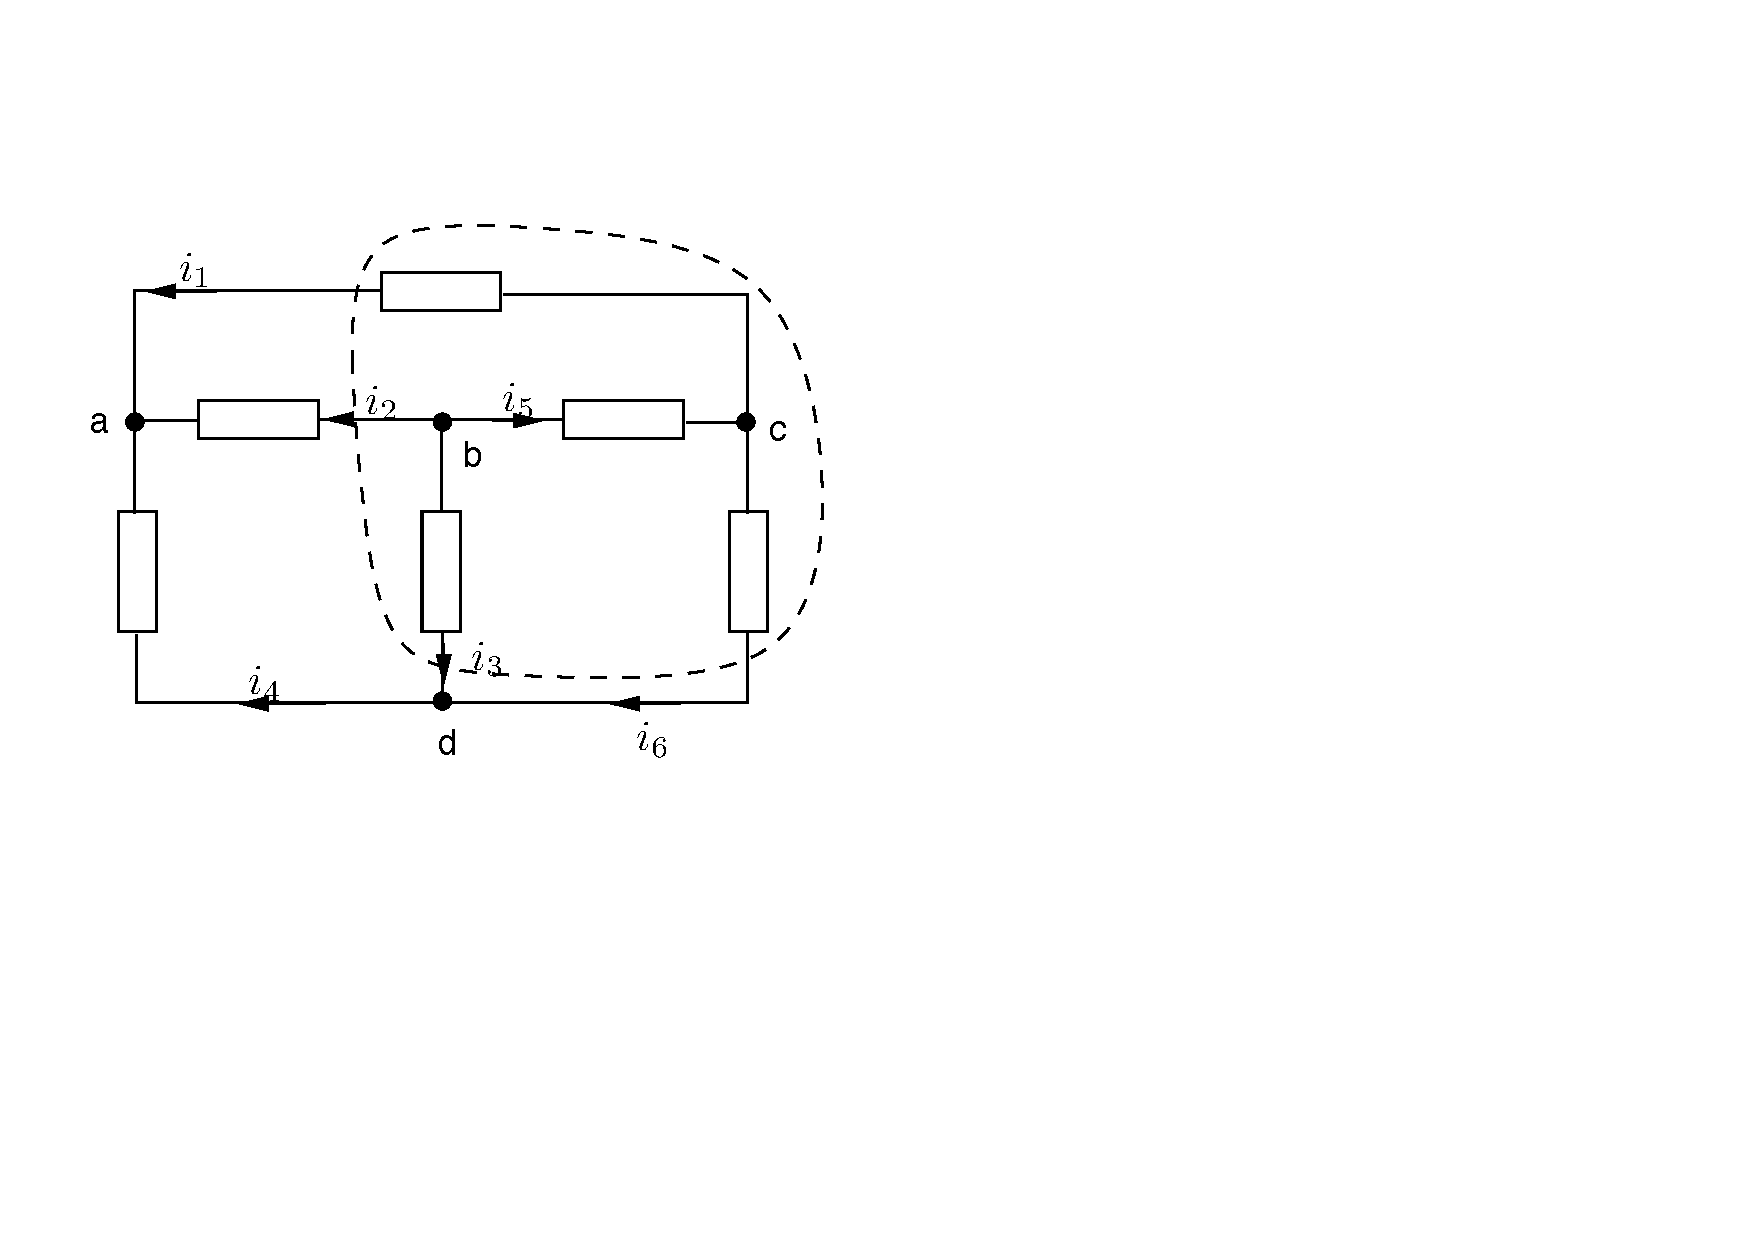
\includegraphics[width=0.6\linewidth]{figs/ch2_figs/plk2ch2}
\end{center}
on a
\[ \begin{array}{lrclr}
\text{noeud a :~}&-i_1-i_2-i_4& =& 0 & (1)\\
\text{noeud b :~}&i_2 + i_3 + i_5 & = & 0& (2)\\
\text{noeud c :~}&i_1 -i_5 +i_6 & = & 0 & (3)\\
\text{noeud d :~}&i_4-i_3-i_6 & = & 0& (4)
\end{array}\]
Et donc 
\begin{center}
(2) + (3) $\Longrightarrow i_1+i_2+i_3+i_6 = 0$
\end{center}
Tout est comme si on avait consid�r� uniquement les courants traversant la coupe en trait interrompu.
\end{testexample}

\subsection{Seconde loi de Kirchhoff (SLK) ou loi des mailles}
La Table~\ref{tab:SLK} �nonce la seconde loi, illustr�e � la Figure~\ref{fig:SLK}.
\begin{table}[h]
	\caption{Seconde loi de Kirchhoff.\label{tab:SLK}}
\begin{boxedminipage}{\textwidth}
{Pour tout circuit localis�, la somme alg�brique des tensions aux
	bornes de toutes les branches constituant une maille est nulle �
	tout instant.}
\begin{equation}
\sum_{b\in \cal{M}}u_b(t)=0 \label{eq:SLK}
\end{equation}
\end{boxedminipage}
\end{table}
\begin{marginfigure}
	\centering
	\begin{tikzpicture}[y=-1cm]
\sf
\filldraw[black] (3.49778,3.20444) circle (0.06667cm);
\filldraw[black] (6.02,3.20444) circle (0.06667cm);
\filldraw[black] (6.02,5.48889) circle (0.06667cm);
\filldraw[black] (3.51111,5.48889) circle (0.06667cm);
\draw[black] (4.5,3.04444) rectangle (5.47778,3.35556);
\draw[black] (3.34444,4.93333) rectangle (3.65556,3.95556);
\draw[black] (5.85556,4.93333) rectangle (6.16667,3.95556);
\draw[black] (3.51111,4.94444) -- (3.51111,5.51111);
\draw[black] (3.48889,3.2) -- (4.5,3.2);
\draw[black] (3.5,3.94444) -- (3.5,3.21111);
\draw[black] (5.5,3.22222) -- (5.98889,3.22222);
\draw[black] (6,3.96667) -- (6,3.22222);
\draw[black] (3.52222,5.52222) -- (2.97778,5.86667);
\draw[black] (6.02222,5.51111) -- (6.81111,6.1);
\draw[black] (6.02222,3.24444) -- (6.46667,2.66667);
\draw[black] (3.51111,3.18889) -- (3.12222,2.61111);
\draw[black] (4.5,5.32222) rectangle (5.47778,5.63333);
\draw[black] (3.51111,5.51111) -- (4.51111,5.51111);
\draw[black] (5.5,5.48889) -- (6.02222,5.48889) -- (6.02222,4.93333);
\path (3.03333,3.82222) node[text=black,anchor=base] {+};
\path (3.1,5.23333) node[text=black,anchor=base] {-};
\path (4.23333,2.98889) node[text=black,anchor=base] {+};
\path (5.61111,2.93333) node[text=black,anchor=base] {-};
\path (6.3,3.88889) node[text=black,anchor=base] {+};
\path (6.26667,5.3) node[text=black,anchor=base] {-};
\path (4.16667,6.01111) node[text=black,anchor=base] {+};
\path (5.63333,6) node[text=black,anchor=base] {-};
\path (4.86667,2.88889) node[text=black,anchor=base] {$u_b$};

\end{tikzpicture}%

%% Configure (x)emacs for this file ...
%% Local Variables:
%% mode: latex
%% End:
	\caption{Seconde loi de Kirchhoff.\label{fig:SLK}}
\end{marginfigure}

\begin{testexample}[SLK.]
Par exemple, dans la figure ci-dessous 
\begin{center}
	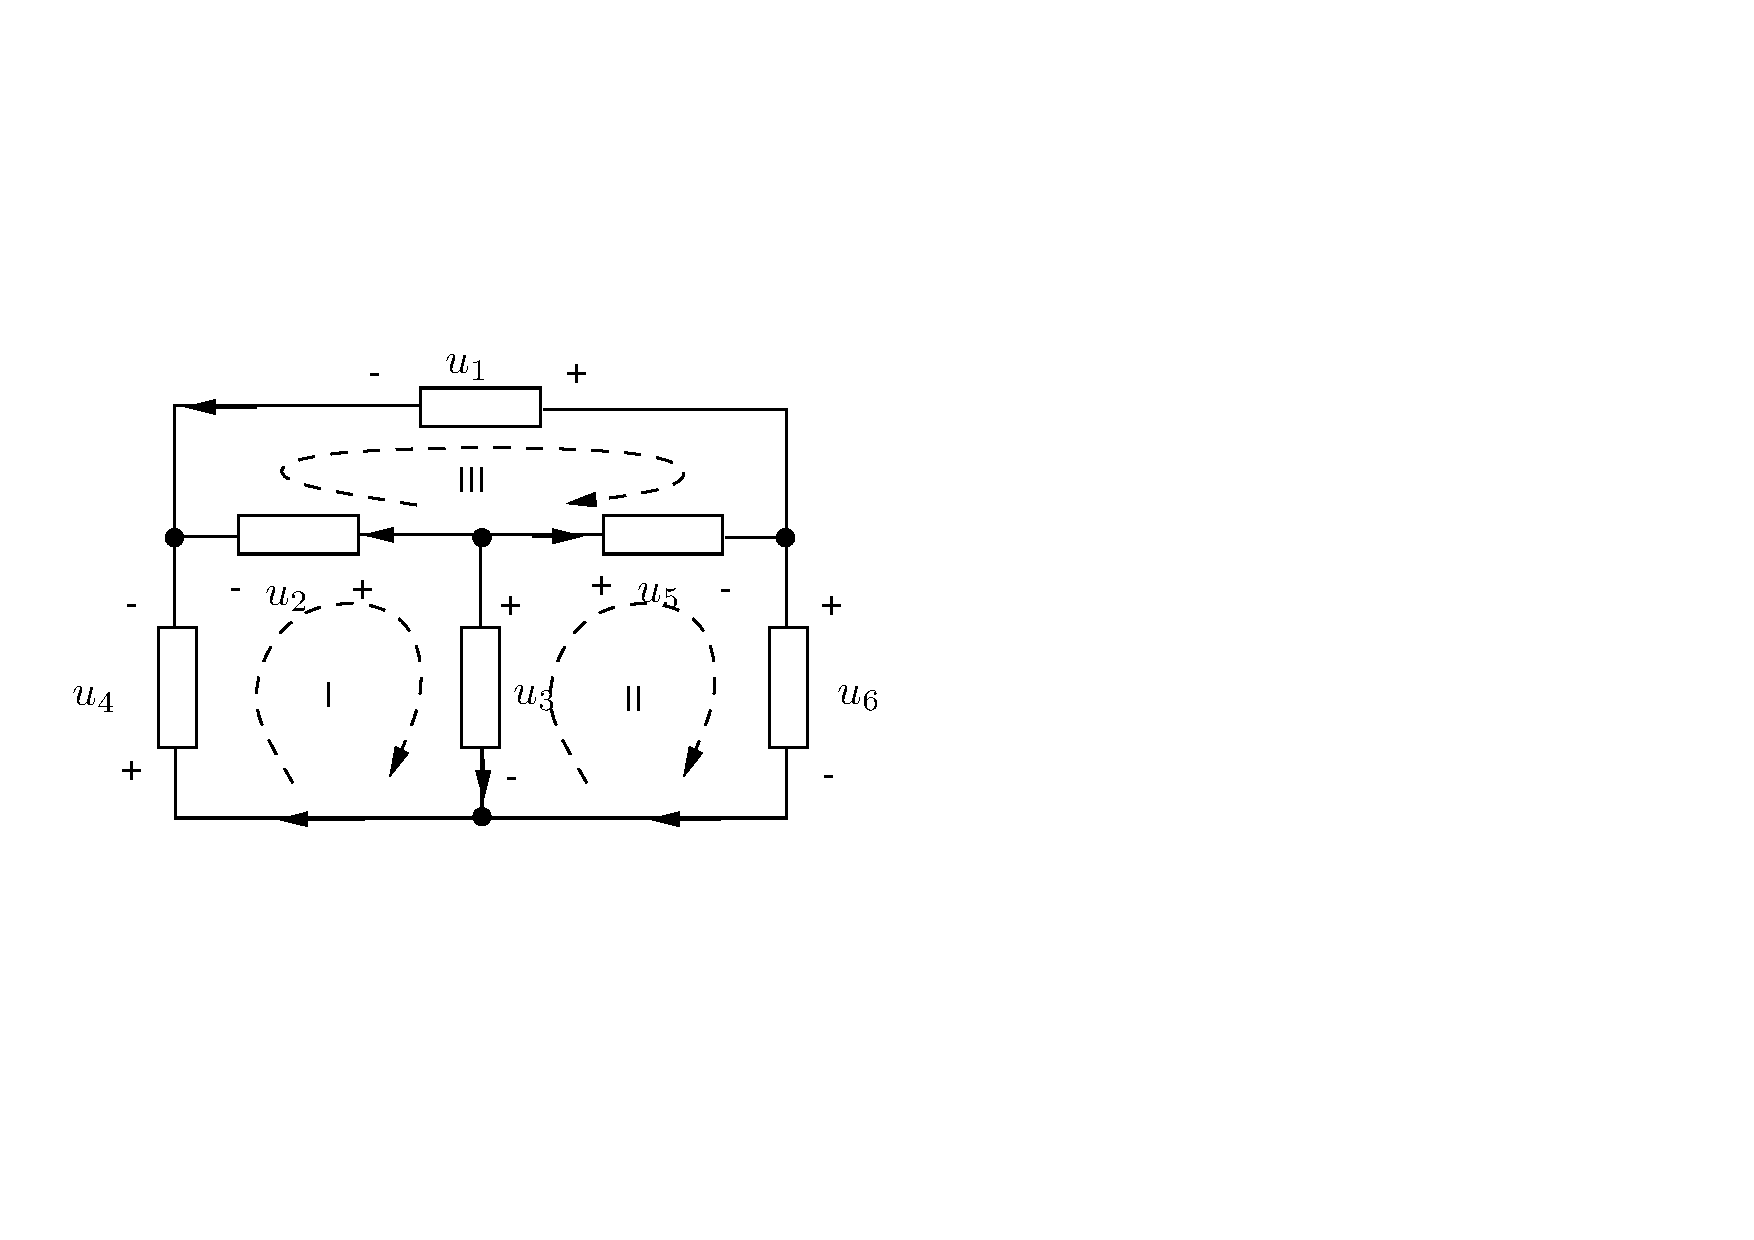
\includegraphics[width=0.7\linewidth]{figs/ch2_figs/SLK}
\end{center}
on a 
\[ \begin{array}{lrcl}
\text{maille I :~}&-u_4+u_2-u_3& =& 0 \\
\text{maille II :}&u_3-u_5-u_6 & = & 0 \\
\text{maille III :}&-u_2+u_1+u_5& = & 0  
\end{array}\]
\end{testexample}

\paragraph{D�monstration.}
La SLK est bas�e sur l'hypoth�se 2 ci-dessus, l'identit� entre d.d.p. et tension dans le cadre des circuits localis�s. Ce qui suit permet de clarifier son interpr�tation. 
En toute g�n�ralit�, le champ �lectrique s'exprime par 
$$\vec{\nabla} \times \overrightarrow{E}  = 
- \frac{\partial \overrightarrow{B}}{\partial t}$$
Donc, en d�finissant $\overrightarrow{B} = \vec{\nabla} \times \overrightarrow{A}$ ($\overrightarrow{A}$ est appel� "potentiel vecteur"), 
$$\overrightarrow{E} =-\vec{\nabla} V -\frac{\partial \overrightarrow{A}}{\partial t}$$
\begin{marginfigure}
\begin{center}
	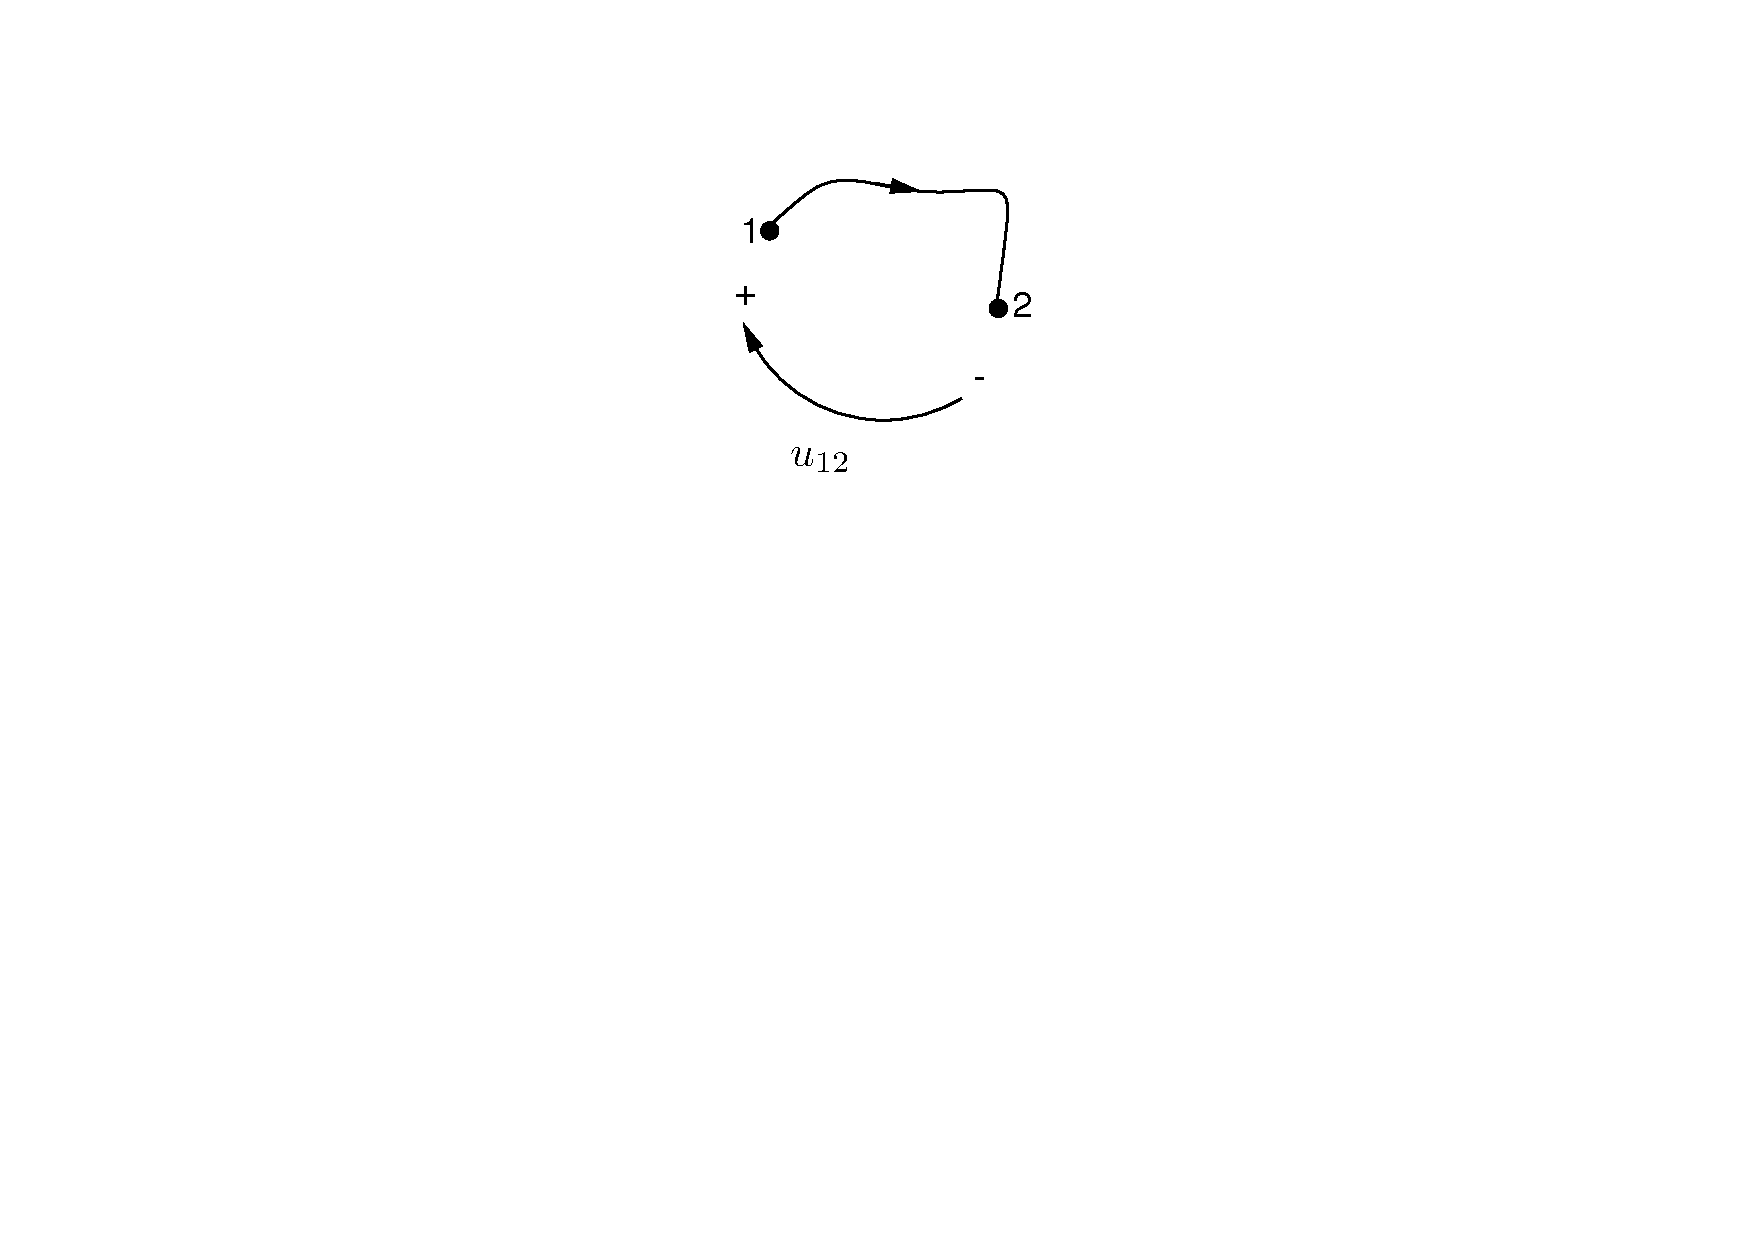
\includegraphics[width=0.7\linewidth]{figs/ch2_figs/tensionch2}
\end{center}
\caption{Tension et d.d.p.} \label{fig:int_ligne}
\end{marginfigure}
L'int�grale de ligne de ce champ fournit par d�finition la tension. Ainsi, par exemple,
dans le cas de la Figure~\ref{fig:int_ligne} , la tension $u_{12}$ entre les noeuds $1$ et $2$ s'exprime par :
 \[u_{12}= \int_1^2\overrightarrow{E}.\overrightarrow{d\ell} = v_1-v_2 - 
\frac{\partial}{\partial t}\int_1^2
\overrightarrow{A}.\overrightarrow{d\ell}\]
Dans le cas g�n�ral, tension et diff�rence de potentiel ne co�ncident pas.
Une des cons�quences pratiques de la prise en consid�ration du terme $\frac{\partial \overrightarrow{A}}{\partial t}$ r�side dans le fait que la mesure � l'aide d'un voltm�tre de la tension entre deux noeuds n'est pas univoquement �valu�e, mais d�pend de la longueur et de la forme des fils
�lectriques reliant ces noeuds au voltm�tre.

Sur un parcours ferm� $123$ (Figure~\ref{fig:int_contour}), on d�rive :
\begin{eqnarray*}
u_{12}+u_{23}+u_{31} & = & 
\oint_{\cal C} \vec{E} . \vec{d\ell} = \int_S (\vec{\nabla} \times \vec{E}).\vec{dS}\\
 & = & 
- \frac{\partial}{\partial t}\int_S  \overrightarrow{B}.\overrightarrow{dS}
=  -\frac{\partial \phi}{\partial t}
\end{eqnarray*}
Or si on est en r�gime � courant continu, $\frac{d}{dt}=0$, et sinon, sous l'hypoth�se des circuits localis�s,  $\frac{\partial
\overrightarrow{B}}{\partial t}\simeq 0$ en dehors des �l�ments.
\begin{marginfigure}
	\begin{center}
	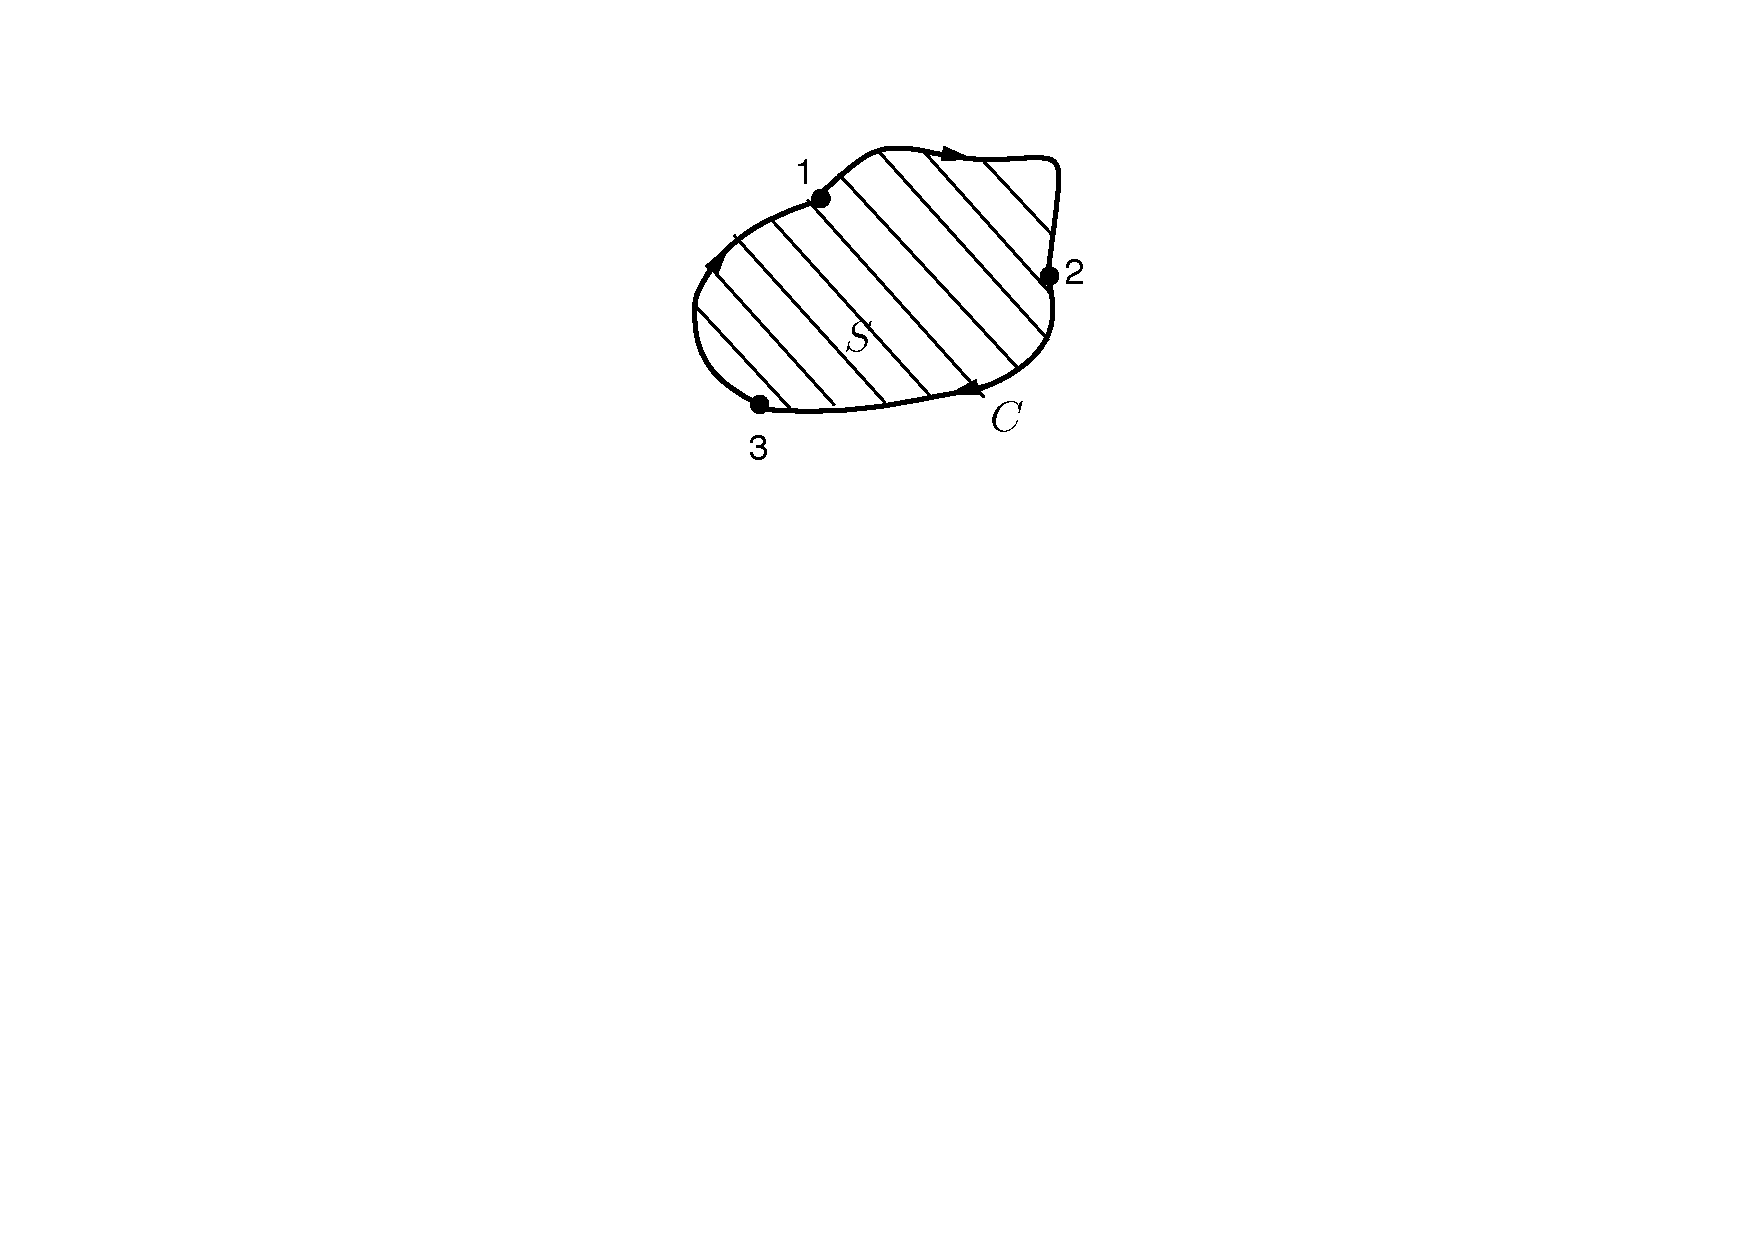
\includegraphics[width=0.7\linewidth]{figs/ch2_figs/contour_ferme}
	\end{center}
	\caption{Contour ferm�.} \label{fig:int_contour}
\end{marginfigure}

\paragraph{R�gle d'application de la SLK � une maille.}
\begin{enumerate}
\item  Fixer un sens de r�f�rence pour les d.d.p. aux bornes des �l�ments des branches de
la maille.
\item  Fixer arbitrairement un sens de circulation de la maille.
\item  Appliquer la relation (\ref{eq:SLK}) en partant d'un point "neutre" du circuit (c'est-�-dire
situ� � l'ext�rieur de ses �l�ments localis�s), en parcourant la maille dans le sens de
circulation choisi et en comptant positivement la d.d.p. aux bornes des �l�ments chaque
fois que l'on rencontre d'abord la borne "$-$", n�gativement dans le cas contraire.
\end{enumerate}

\section{Loi d'Ohm}
\label{sec:ohm}

D�montr�e dans le cas du r�gime stationnaire � partir de la th�orie cin�tique des gaz d'abord, valid�e par la m�canique quantique ensuite, la loi d'Ohm locale s'�crit (en r�gime stationnaire):
$$\overrightarrow{J}=\sigma \overrightarrow{E},$$ 
o� $\sigma$ est la conductivit� �lectrique du conducteur. C'est un scalaire dans le cas des conducteurs m�talliques
homog�nes) : 
$$\sigma=\frac{ne^2\lambda}{mv}$$
avec 
\begin{center}
	\begin{tabular}{rl}
		$n$& le nombre d'�lectrons par unit� de volume \\
		$e$& la charge de l'�lectron \\
		$\lambda$& le libre parcours moyen des �lectrons \\
		$v$&la vitesse moyenne des �lectrons \\
		$m$&la masse de l'�lectron. \\
	\end{tabular}
\end{center}

La loi d'Ohm globale s'en d�duit ais�ment : pour un conducteur de longueur $\ell$, de section (constante) $S$ et de conductivit� $\sigma$, parcouru par un courant continu $I$, on trouve (voir Figure~\ref{fig:ohm-globale}) :
\begin{marginfigure}
	\centering
	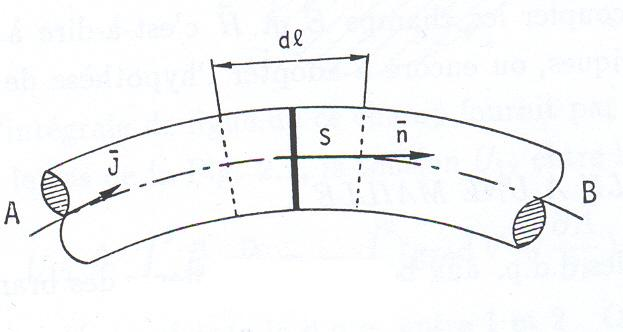
\includegraphics[width=6cm]{figs/ch2_figs/resis.jpg}
	\caption{Loi d'Ohm globale.} \label{fig:ohm-globale}
\end{marginfigure}
$$U=V_A-V_B=\int_A^B \overrightarrow{E}.\overrightarrow{d\ell}= RI 
$$
o� 
$$R = \displaystyle \frac{\ell}{\sigma S}$$ est la r�sistance de l'�l�ment.\footnote{Par extension, la loi d'Ohm est utilis�e en r�gime quasi-stationnaire, o� cependant l'effet pelliculaire peut introduire des modifications non-n�gligeables. Notons �galement qu'appliqu�e au cas d'un semi-conducteur ou d'un plasma plong� dans une induction
	magn�tique, la loi d'Ohm doit �tre corrig�e pour tenir compte de l'effet Hall.}

\section{La r�sistance}

Une r�sistance de r�sistance $R$\footnote{� noter la pauvret� du fran�ais � cet �gard: r�sistance d�signe tout aussi bien l'�l�ment physique
(en anglais "resistor") que la valeur �lectrique le caract�risant (en anglais "resistance").} est un dip�le qui, parcouru par un courant, fait
na�tre � ses bornes une d.d.p. fonction de ce courant. 
\[u(t)=R\, i(t)\]

$R$ s'exprime en Ohm ($\Omega$).
Une r�sistance peut �tre lin�aire ou non, variante ou invariante (quatre combinaisons possibles).

En toute g�n�ralit� on a $R=f(u,i,t)$, et les cas particuliers suivants : 
\begin{itemize}
	\item $R=f(u,i)$ : r�sistance {\em autonome} ou {\em invariante}
	les caract�ristiques de l'�l�ment ne d�pendent pas du temps
	\item $R=f(t)$ : r�sistance {\em lin�aire}
	\item $R= constante$ : r�sistance {\em lin�aire et invariante}.
\end{itemize}

\begin{marginfigure}
\begin{center}
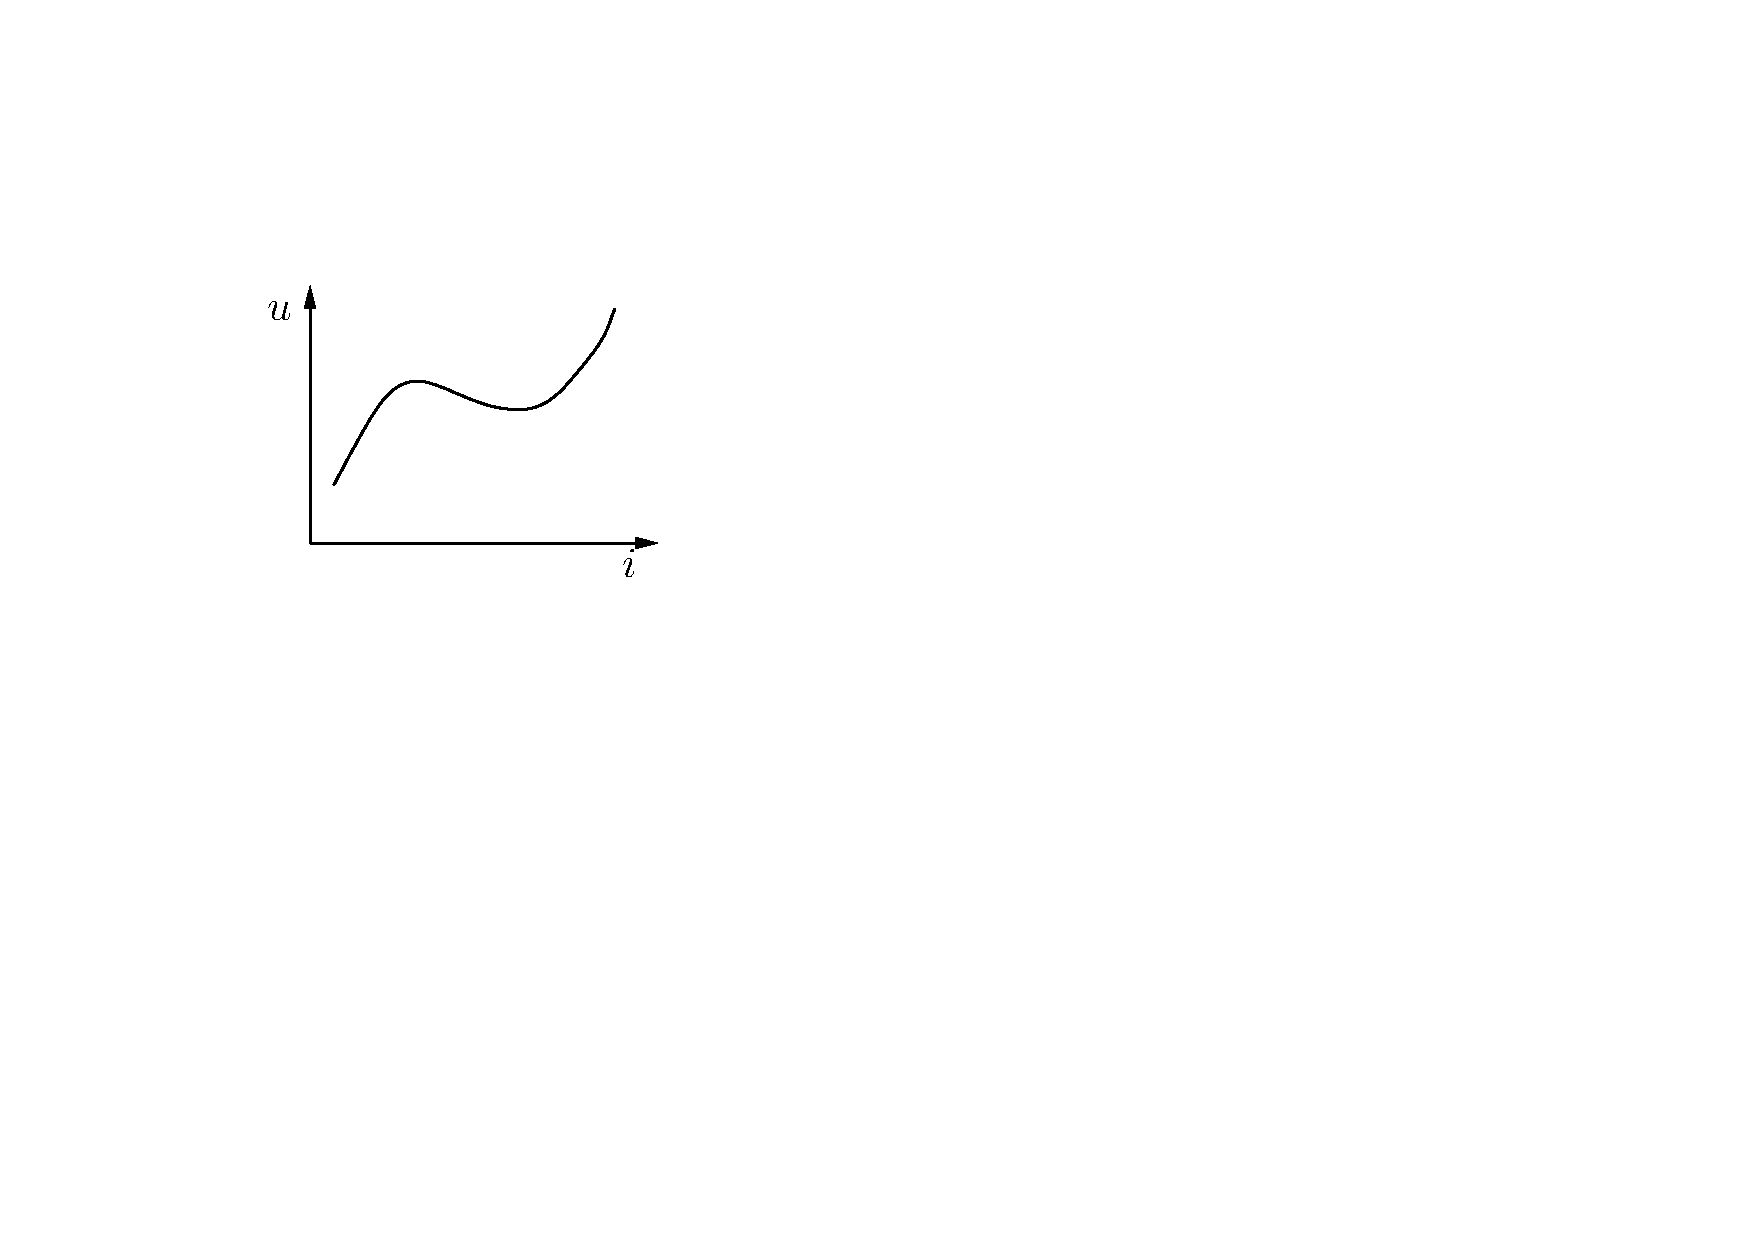
\includegraphics[width=0.65\linewidth]{figs/ch2_figs/RNL}
\end{center}
\caption{R�sistance non lin�aire}
\end{marginfigure}
\begin{marginfigure}
	\centering
	\begin{tikzpicture}[y=-1cm]
\sf
\draw[arrows=-triangle 45,black] (2.60222,3.34222) -- (2.60222,1.23333);
\draw[arrows=-triangle 45,black] (2.60222,3.33556) -- (5.44444,3.33556);
\draw[black] (2.61111,3.31111) -- (5.13333,2.03333);
\path (2.45111,1.51333) node[text=black,anchor=base east] {$u$};
\path (5.21111,3.61556) node[text=black,anchor=base] {$i$};

\end{tikzpicture}%

%% Configure (x)emacs for this file ...
%% Local Variables:
%% mode: latex
%% End:
	\caption{R�sistance lin�aire. Droite passant par $(0,0)$.
		Pente de la droite = $R$}
\end{marginfigure}
L'hypoth�se de lin�arit� est vraie  dans une plage de fonctionnement seulement. 
Avec l'accroissement de la fr�quence de fonctionnement d'un circuit, l'effet pelliculaire impacte la r�sistance des conducteurs.

\paragraph{Conductance.}
On appelle \textit{conductance} l'inverse de la r�sistance
$$\quad i =\frac{1}{R}u=Gu$$
$G$  s'exprime en Siemens (S).

\paragraph{Association en s�rie.}
Deux r�sistances en s�rie s'additionnent. Consid�rons le circuit de la Figure~\ref{fig:serie}.
\begin{marginfigure}
	\centering
	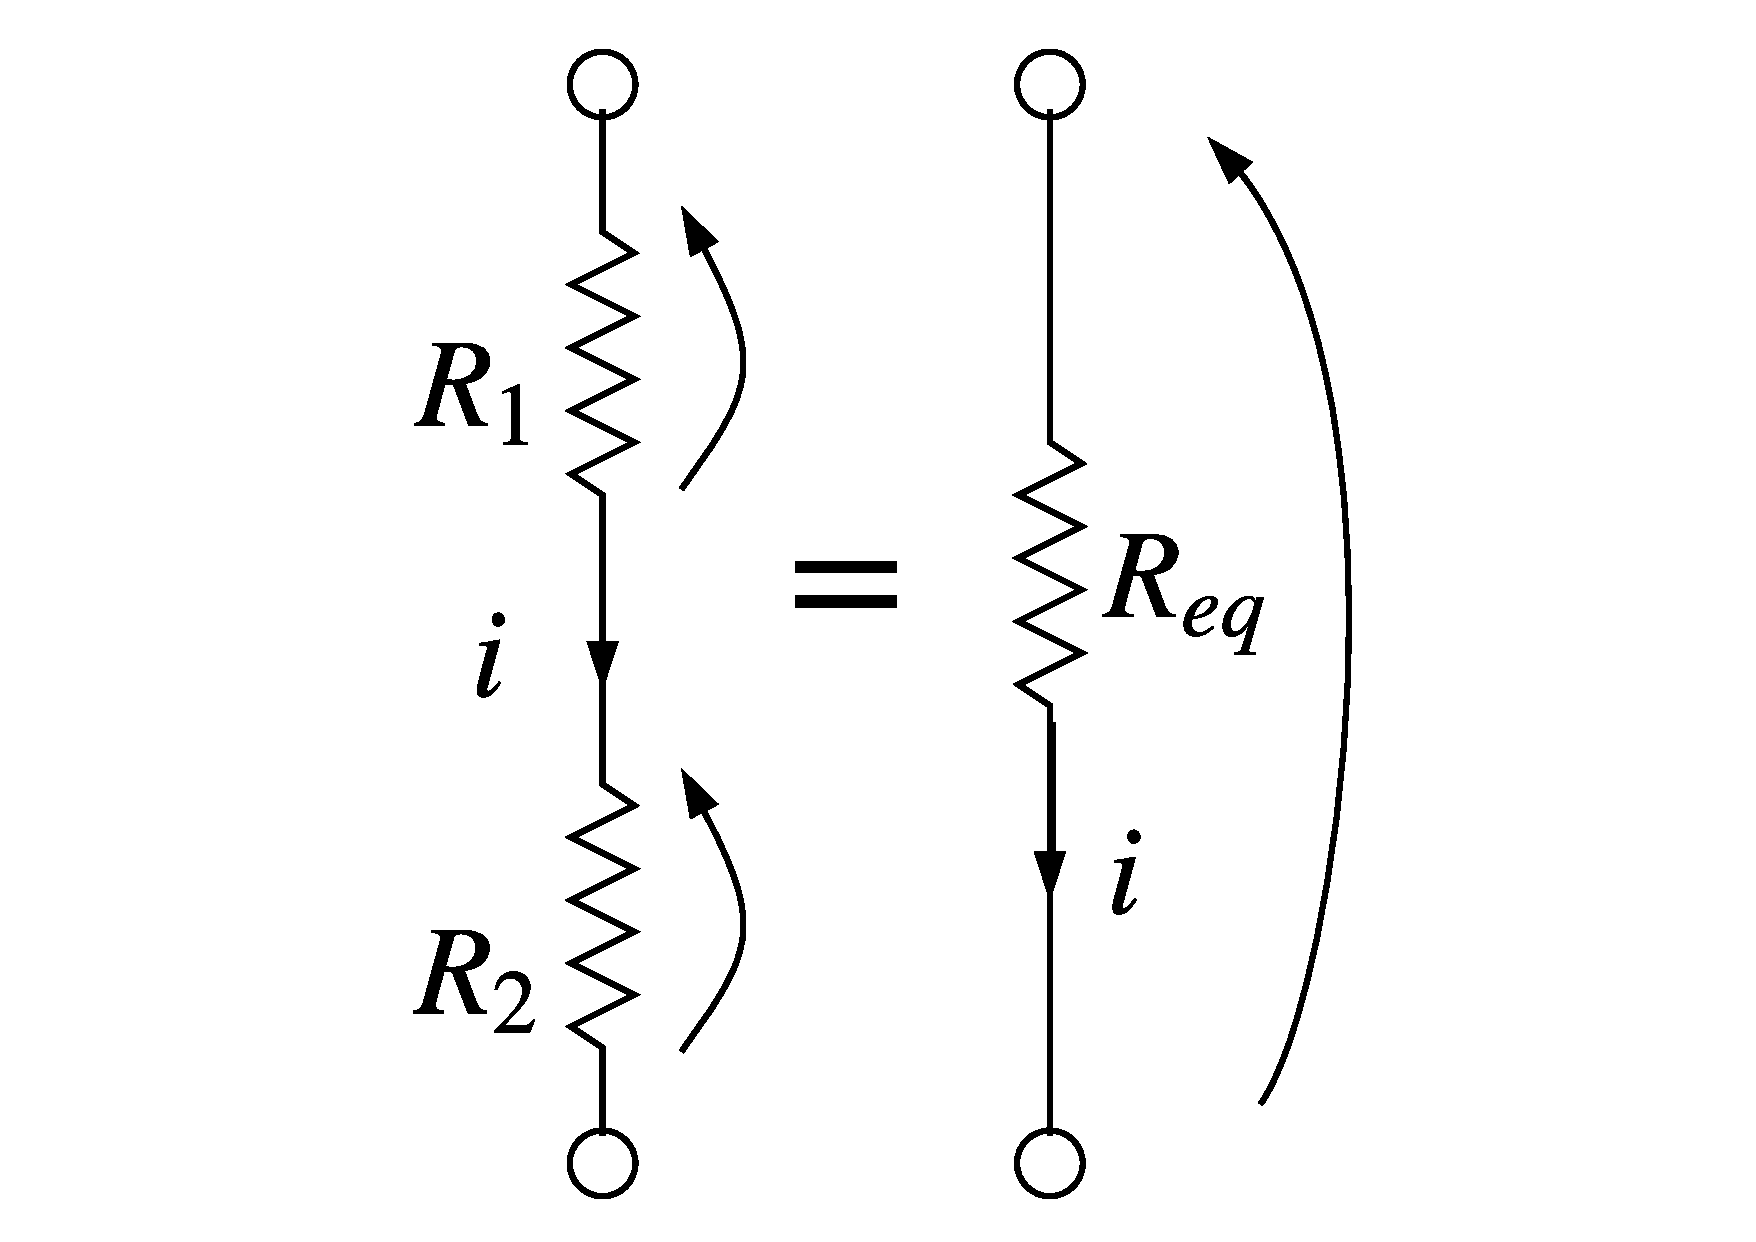
\includegraphics[width=0.98\linewidth]{figs/ch2_figs/serie}
	\caption{Association en s�rie.}
	\label{fig:serie}
\end{marginfigure}
Le courant $i$ traverse les deux r�sistances. La r�sistance �quivalente $R_{eq}$ doit provoquer la m�me chute de tension que la mise en s�rie des deux r�sistances.
On a $v_{R_1} = R_1 i$ et $v_{R_2} = R_2 i$. La chute de tension aux bornes de la r�sistance �quivalente  est $$v_{R_{eq}} = R_{eq} i = v_{R_1} + v_{R_2} = (R_1+R_2) i.$$ 
Donc $$R_{eq} = R_{1} + R_2.$$
Plus g�n�ralement, la r�sistance �quivalente $R_{eq}$ � $n$ r�sistances en s�rie $R_1, R_2, ..., R_n$ est �gale � $$R_{eq} = \sum_{i=1}^n R_i.$$
Si on utilise la conductance des (�l�ments) r�sistances, on a alors 
$$G_{eq} = \left(\sum_{i=1}^n \frac{1}{G_i}\right)^{-1} = R_{eq}^{-1}.$$

\paragraph{Association en parall�le.}

Deux conductances en parall�le s'additionnent. Consid�rons le circuit de la Figure~\ref{fig:serie}.
Soit $G_1 = R_1^{-1}$ et $G_2 = R_2^{-1}$. Par d�finition de la mise en parall�le, la diff�rence de potentiel $v$ est la m�me aux bornes des deux �l�ments.  La r�sistance �quivalente $R_{eq}$ doit �tre travers�e par le m�me courant  que la mise en parall�le des deux r�sistances.
\begin{marginfigure}
	\centering
	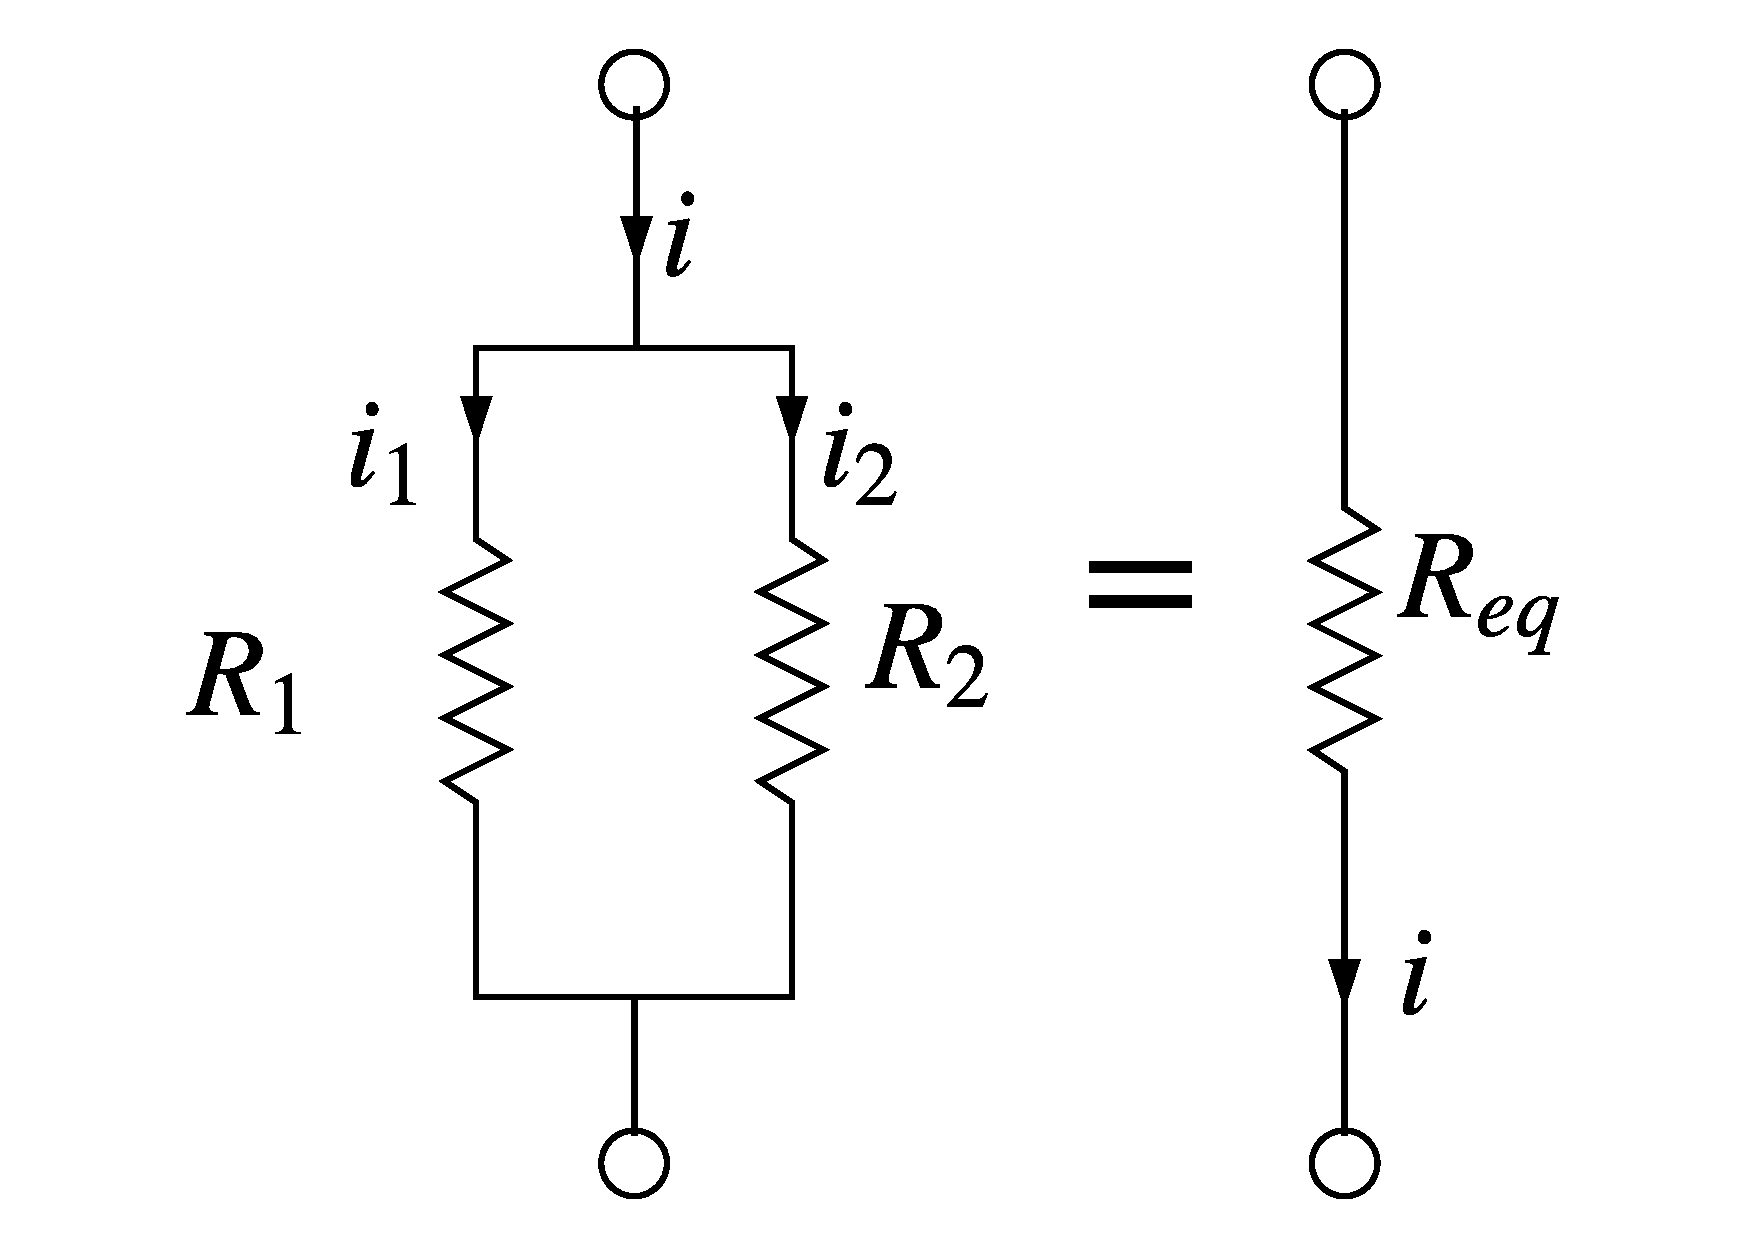
\includegraphics[width=0.98\linewidth]{figs/ch2_figs/parallele}
	\caption{Association en parall�le.}
	\label{fig:parallele}
\end{marginfigure}
On a $i_1 = G_1 v$ et $i_2 = G_2 v$. Le courant dans la r�sistance �quivalente  est $$i = G_{eq} v = i_1 + i_2 = (G_1+G_2) v.$$ 
Donc $$G_{eq} = G_{1} + G_2, $$
ou $$R_{eq} = \left(\frac{1}{R_1}+\frac{1}{R_2}\right)^{-1} = \frac{R_1R_2}{R_1+R_2}.$$
Plus g�n�ralement, la conductance �quivalente $G_{eq}$ � $n$ conductances en parall�le $G_1, G_2, ..., G_n$ est �gale � $$G_{eq} = \sum_{i=1}^n G_i.$$

\paragraph{En pratique.}
La Figure~\ref{fig:Resistors} illustre quelques r�sistances marqu�es en utilisant un syst�me de rep�rage normalis� qui permet de d�duire la valeur des composant et leur degr� de pr�cision. 
\begin{figure}[htb]
	\centering
	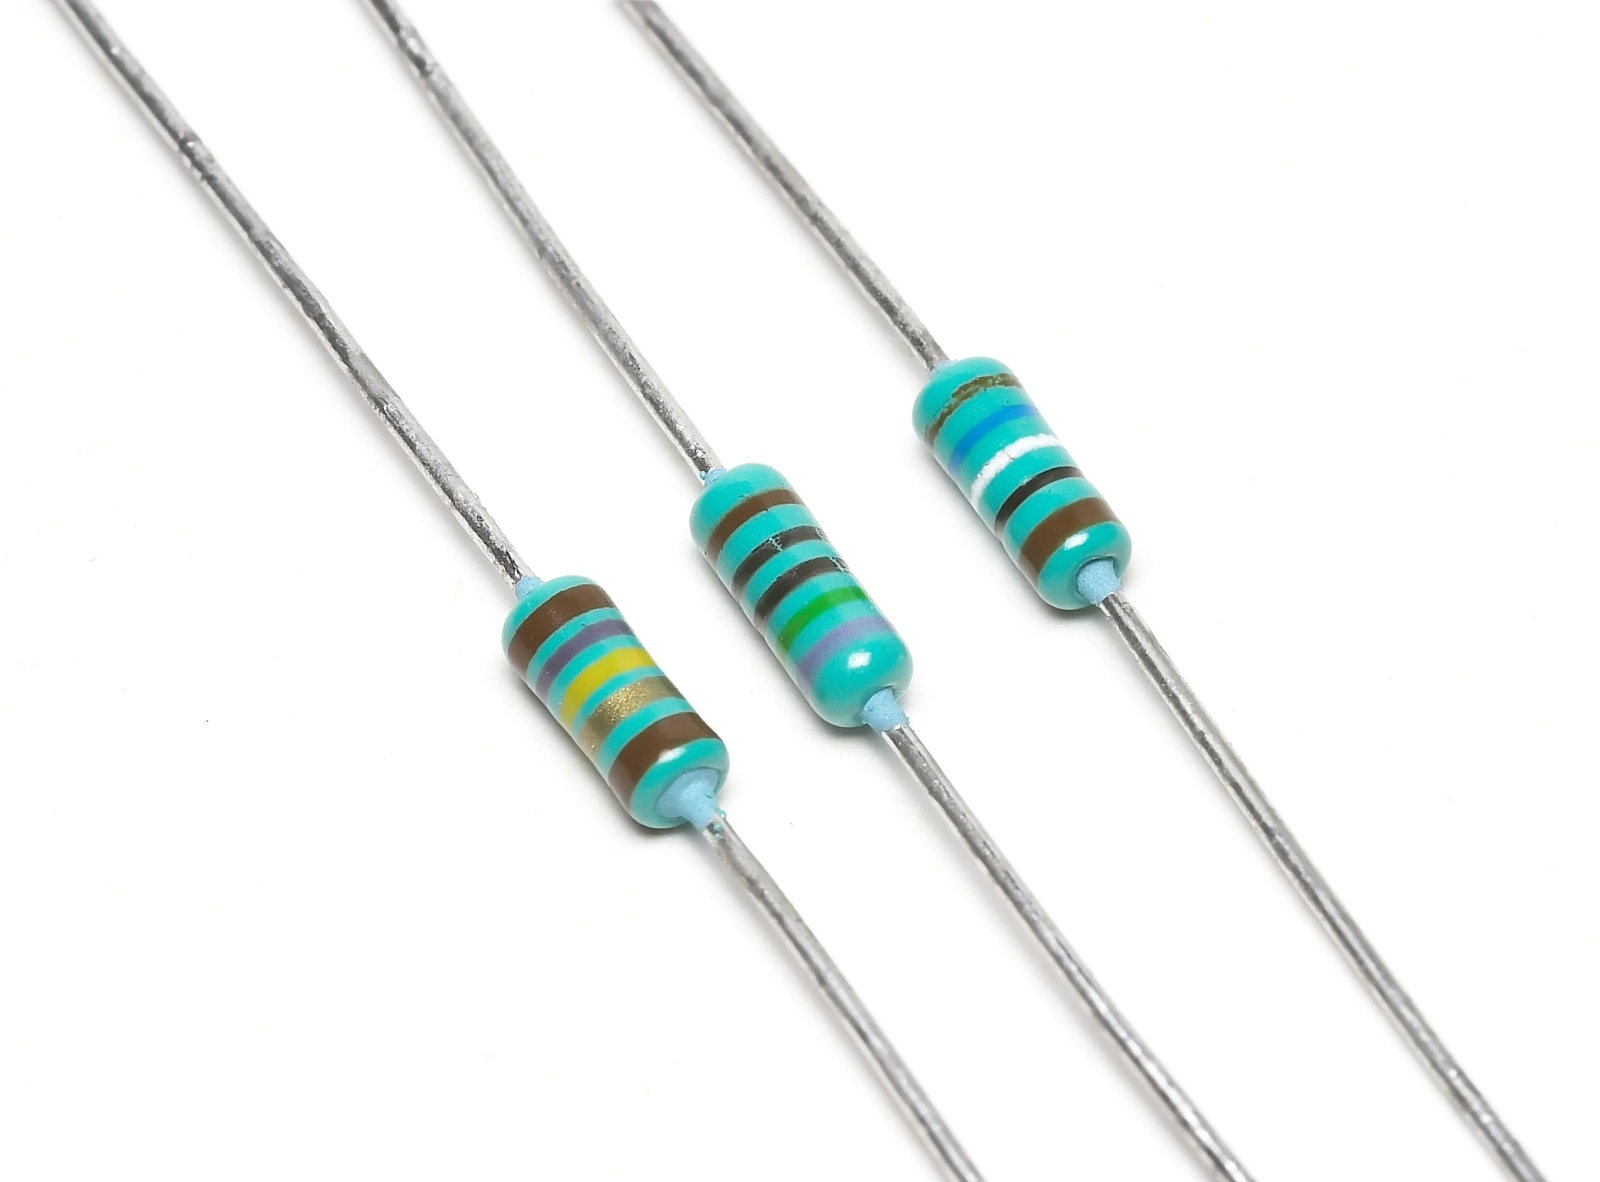
\includegraphics[width=0.68\linewidth]{figs/ch2_figs/Resistors}
	\caption[Exemples de r�sistances marqu�es selon la norme CEI 60757.]{Exemples de r�sistances marqu�es selon la norme CEI 60757. Source: Wikipedia \url{https://fr.wikipedia.org/wiki/Resistance_(composant)}.}
	\label{fig:Resistors}
\end{figure}
Les r�sistances se d�clinent en pratique selon de nombreuses formes, comme par exemple 
\begin{itemize}
\item les r�sistances au carbone,
\item les r�sistances � film m�tallique,
\item le potentiom�tre : r�sistance variable,
\item les photor�sistances : $R$ d�pend de l'�clairement (capteur),
\item les thermistances : $R$ d�pend de la temp�rature (capteur).
\end{itemize}

\section{L'inductance}

Un noyau magn�tique entour� d'une bobine de $N$ spires parcourue par un courant continu $I$ fait na�tre dans la bobine un flux $\phi$ (flux total embrass� par toutes les spires).

Une inductance est un dip�le �lectrique caract�ris� par le fait qu'� tout instant le courant
le parcourant et le flux magn�tique associ� sont reli�s par une courbe dans le plan
$(\phi, i)$, c'est pr�cis�ment la courbe caract�ristique de l'inductance � l'instant $t$ :
$$\phi(t) = f[i(t)].$$
\begin{marginfigure}
	\centering
	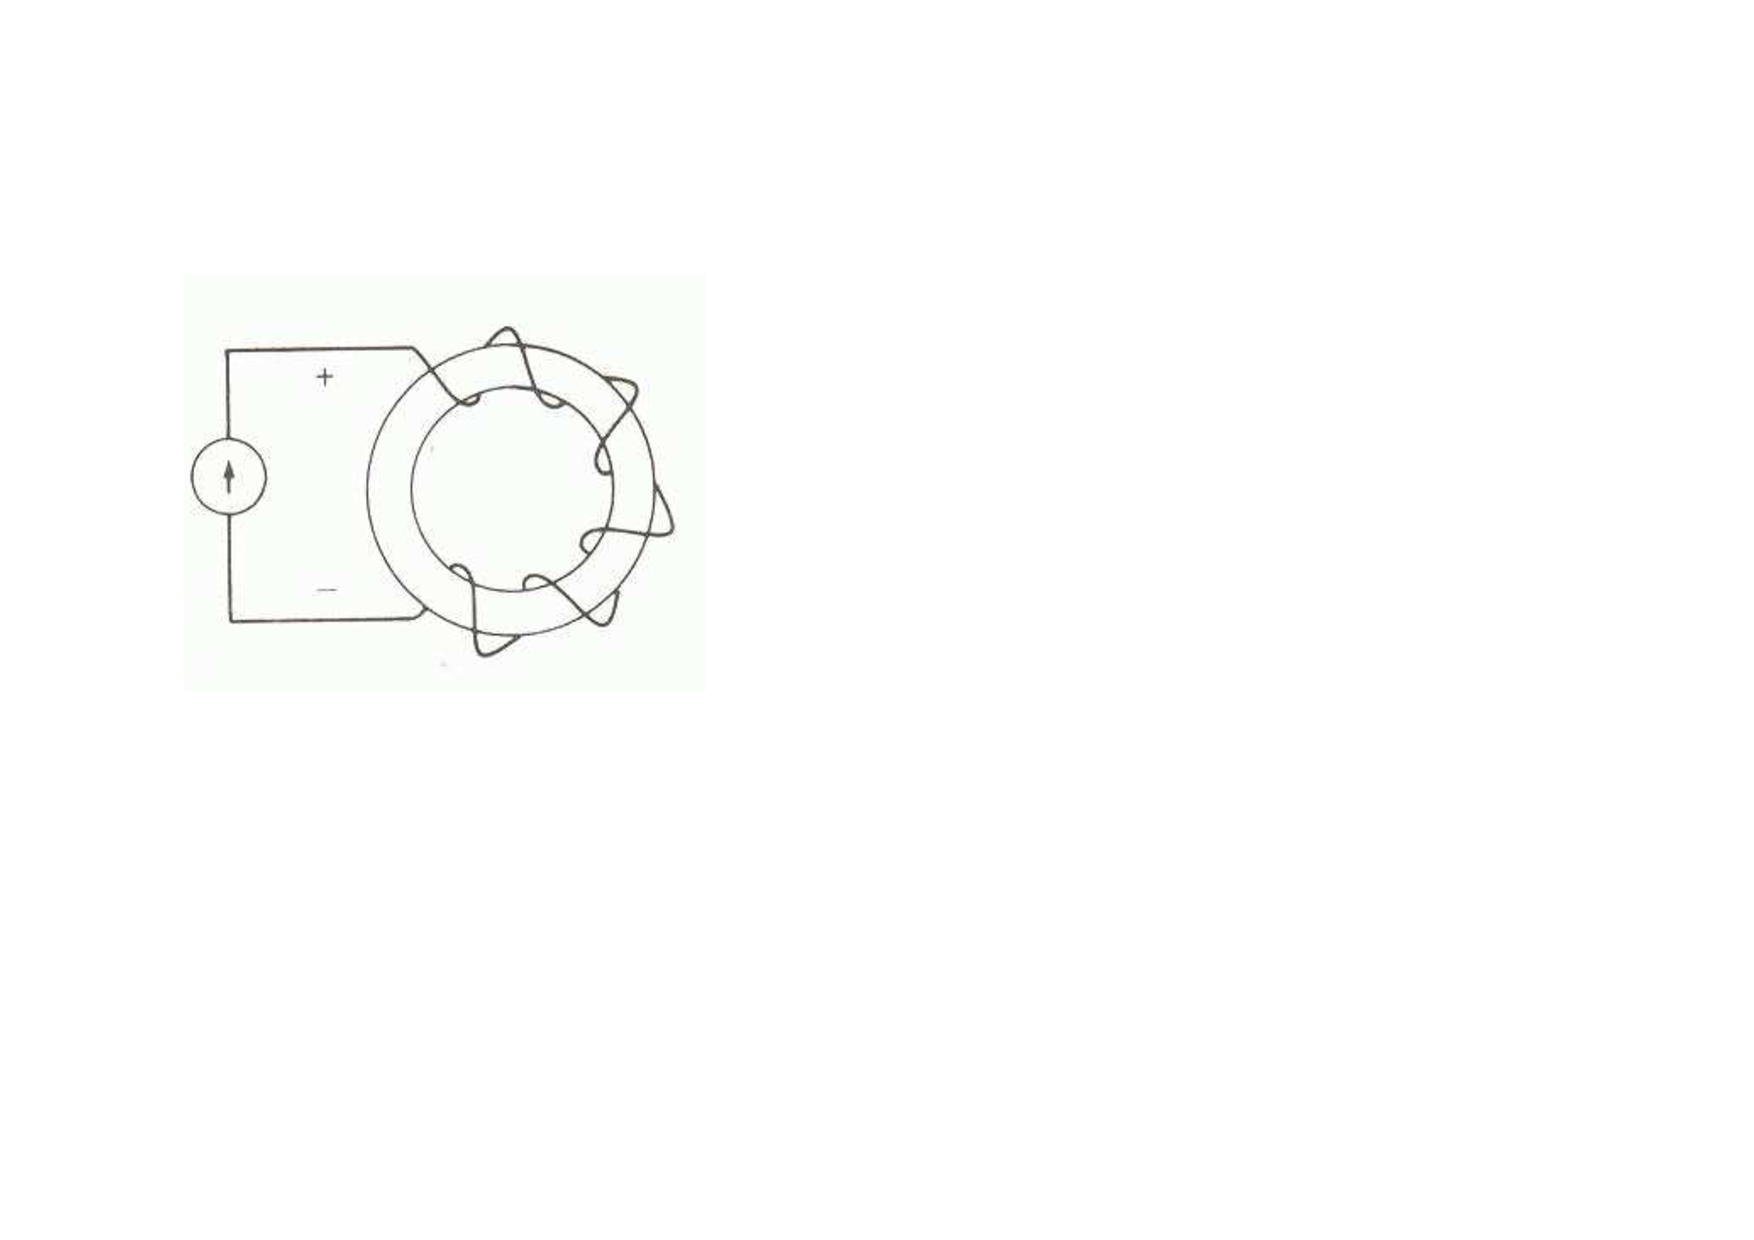
\includegraphics[width=4cm]{figs/figs_reg_trans/bobine.pdf}
	\caption{Bobine.}
\end{marginfigure}
Le coefficient de self-induction d'une bobine de (ou simplement d'un) fil �lectrique
parcouru par un courant est d�fini � un instant donn� comme �tant le rapport entre les
valeurs du flux induit par le courant et de ce courant lui-m�me :
$$\phi(t) = L(t) i(t).$$
En fait, cette relation est une relation lin�aire du point de vue �lectrique et $L(t)$
repr�sente une inductance lin�aire ; sa courbe caract�ristique est une droite passant par
l'origine, mais dont le coefficient angulaire peut �tre temporellement variable.

En pratique dans ce cours nous allons toujours consid�rer l'inductance $L$ lin�aire et invariante, c'est-�-dire constante.
La tension $u(t)$ s'exprime par
$$u(t)=\frac{d\phi(t)}{dt}$$
Donc 
$$u(t)=L\frac{di(t)}{dt}$$
ou encore
$$i(t)=\frac{1}{L}\int_{-\infty}^t u(\tau) d\tau$$
Ces relations sont �tablies selon le sens conventionnel (Figure~\ref{fig:inductance}).
\begin{marginfigure}
	\centering
	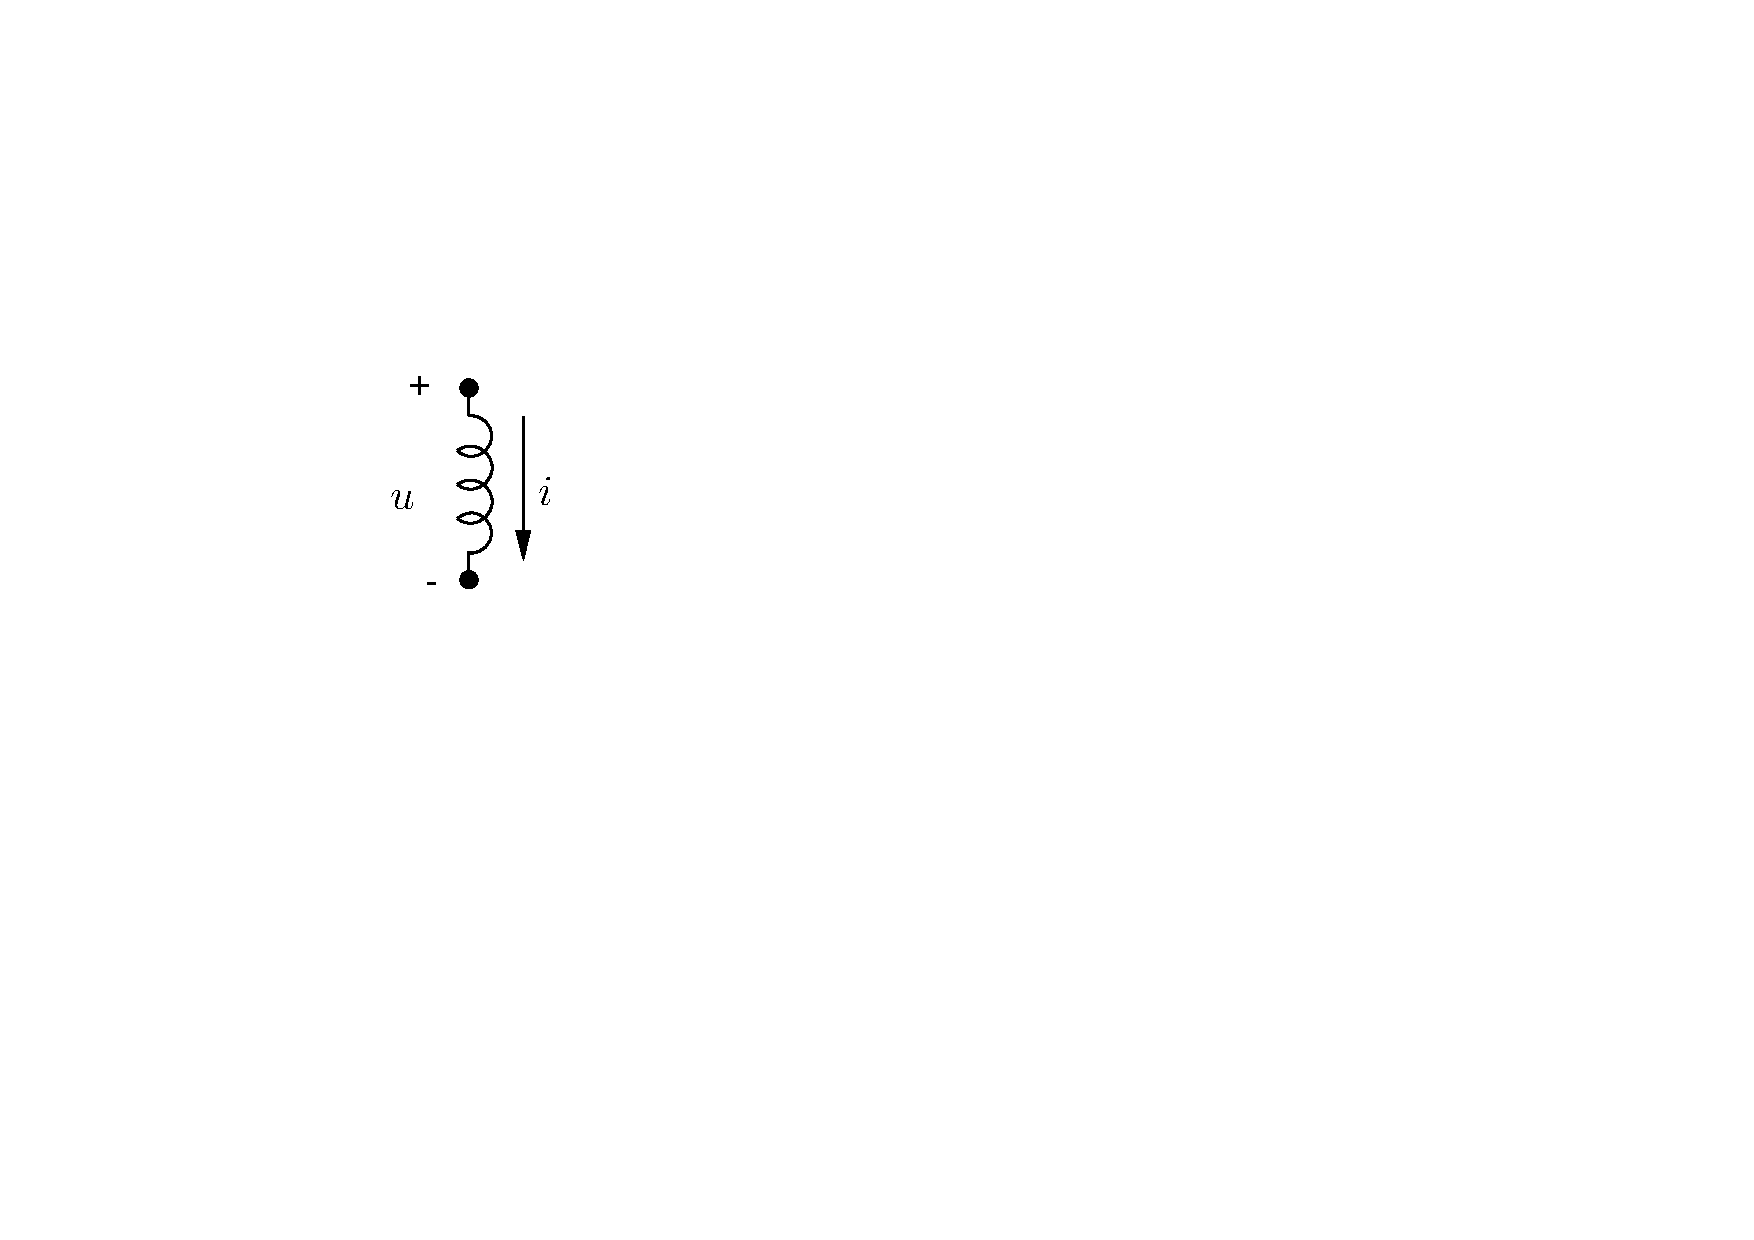
\includegraphics[width=2cm]{figs/figs_reg_trans/symbole_bobine_et_sens.pdf}
	\caption{Symbole et sens conventionnel d'une bobine.} \label{fig:inductance}
\end{marginfigure}

Il existe cependant plusieurs causes de non-lin�arit� telles que l'hyst�r�sis ou la saturation.
En toute g�n�ralit�, on aura donc $L=f(u,i,t)$.
Cas particuliers:
\begin{itemize}
	\item $L=f(u,i)$ : inductance  {\em autonome} ou {\em invariante}
	\[u(t)=L(u,i)\frac{di(t)}{dt},\]
	relation non-lin�aire.
	\item $L=f(t)$ : inductance {\em lin�aire}
	\[u(t)=\frac{dL(t)}{dt}i(t)+L(t)\frac{di(t)}{dt}\]
\end{itemize}

Le coefficient de self-induction s'exprime, en fonction des param�tres physiques de la bobine par 
$$L=\mu \frac{N^2S}{\ell}$$
o� $\mu$ est la perm�abilit� magn�tique du noyau, $S$ est la surface d'une spire et $\ell$ est la longueur de la bobine.
Le coefficient de self-induction s'exprime en henry ($H$).

\subsection{En r�gime non stationnaire}
Une variation du courant et donc du flux implique l'apparition d'une force
contre-�lectromotrice aux bornes de la bobine (loi de Lenz).
Au niveau de la bobine :
\begin{itemize}
	\item le flux qui traverse les spires est variable
	\item selon la loi de Lenz, une {\em force
		contre-�lectromotrice} $\frac{d\phi}{dt}$ appara�t
	\item l'induction magn�tique est variable � l'int�rieur de la bobine
	\[\vec{\nabla} \times \overrightarrow{E}  = -
	\frac{\partial \overrightarrow{B}}{\partial t}\]
\end{itemize}
Ce flux et cette induction magn�tique variables  sont
"confin�s" � l'int�rieur de l'�l�ment, car on a fait l'hypoth�se des circuits
localis�s.

Comme illustr� � la Figure~\ref{fig:inductors}, il existe beaucoup d'impl�mentations physiques d'inductances, tels que le sol�no�de, un enroulement en Cu sur mat�riau ferromagn�tique.
\begin{figure}[tb]
	\centering
	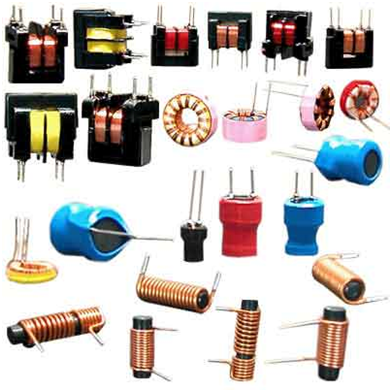
\includegraphics[width=0.68\linewidth]{figs/ch2_figs/inductors}
	\caption[Exemples d'inductances.]{Exemples d'inductances. Source: Wikipedia \url{https://en.wikipedia.org/wiki/Inductor}.}
	\label{fig:inductors}
\end{figure}
Des composants normalis�s existent, mais en moins grand nombre que pour les r�sistances et les condensateurs, et de moins bonne pr�cision.

\paragraph{Remarques.}
Les inductances � noyau ferromagn�tique sont en g�n�ral tributaires du ph�nom�ne
d'hyst�r�sis (Figure~\ref{fig:hysteresis}). La caract�ristique d'un tel �l�ment n'est pas une courbe � proprement parler et la d�finition m�me du dip�le "inductance" n'est plus valable.
Une  technique consiste � mod�liser l'inductance avec noyau par un circuit $RL$ s�rie, o� $R$ mod�lise les pertes par hyst�r�sis
(qui sont proportionnelles � l'aire de la courbe d'hyst�r�sis) et o� $L$ repr�sente une
courbe caract�ristique "moyenne" de l'inductance r�elle.
\begin{marginfigure}
\centering
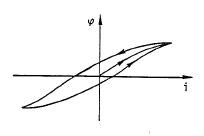
\includegraphics[width=0.9\linewidth]{figs/ch2_figs/hysteresis}
\caption{Courbe d'hyst�r�sis d'une bobine.}
\label{fig:hysteresis}
\end{marginfigure}
Les inductances souffrent �galement de probl�mes de pertes par effet Joule dans le conducteur et de l'effet pelliculaire aux hautes fr�quences.
Dans un circuit, on tentera donc au maximum d'�viter les bobines si possible.

\section{Le condensateur}

Un condensateur est constitu� de deux plaques parall�les conductrices de surface $S$ s�par�es d'une
distance $d$ et portant des charges �gales et oppos�es $\pm q$.
Les charges font na�tre une diff�rence de potentiel $V$ entre les plaques.
Il est caract�ris� par une relation entre la charge �lectrique $(q_+, q_-)$
sur ses plaques et la d.d.p. entre celles-ci (Figure~\ref{fig:condensateur}). 
On d�finit le dip�le condensateur de fa�on analogue � celle de l'inductance. 
Ainsi, si le condensateur est lin�aire, la courbe caract�ristique $q(t) = f[u(t)]$ est une droite passant par l'origine et on �crit :
$$q(t) = C(t) u(t).$$
$C(t)$, le coefficient de proportionnalit� entre $q$ et $u$, est appel� \textit{capacit� du condensateur}.
\begin{marginfigure}
	\centering
	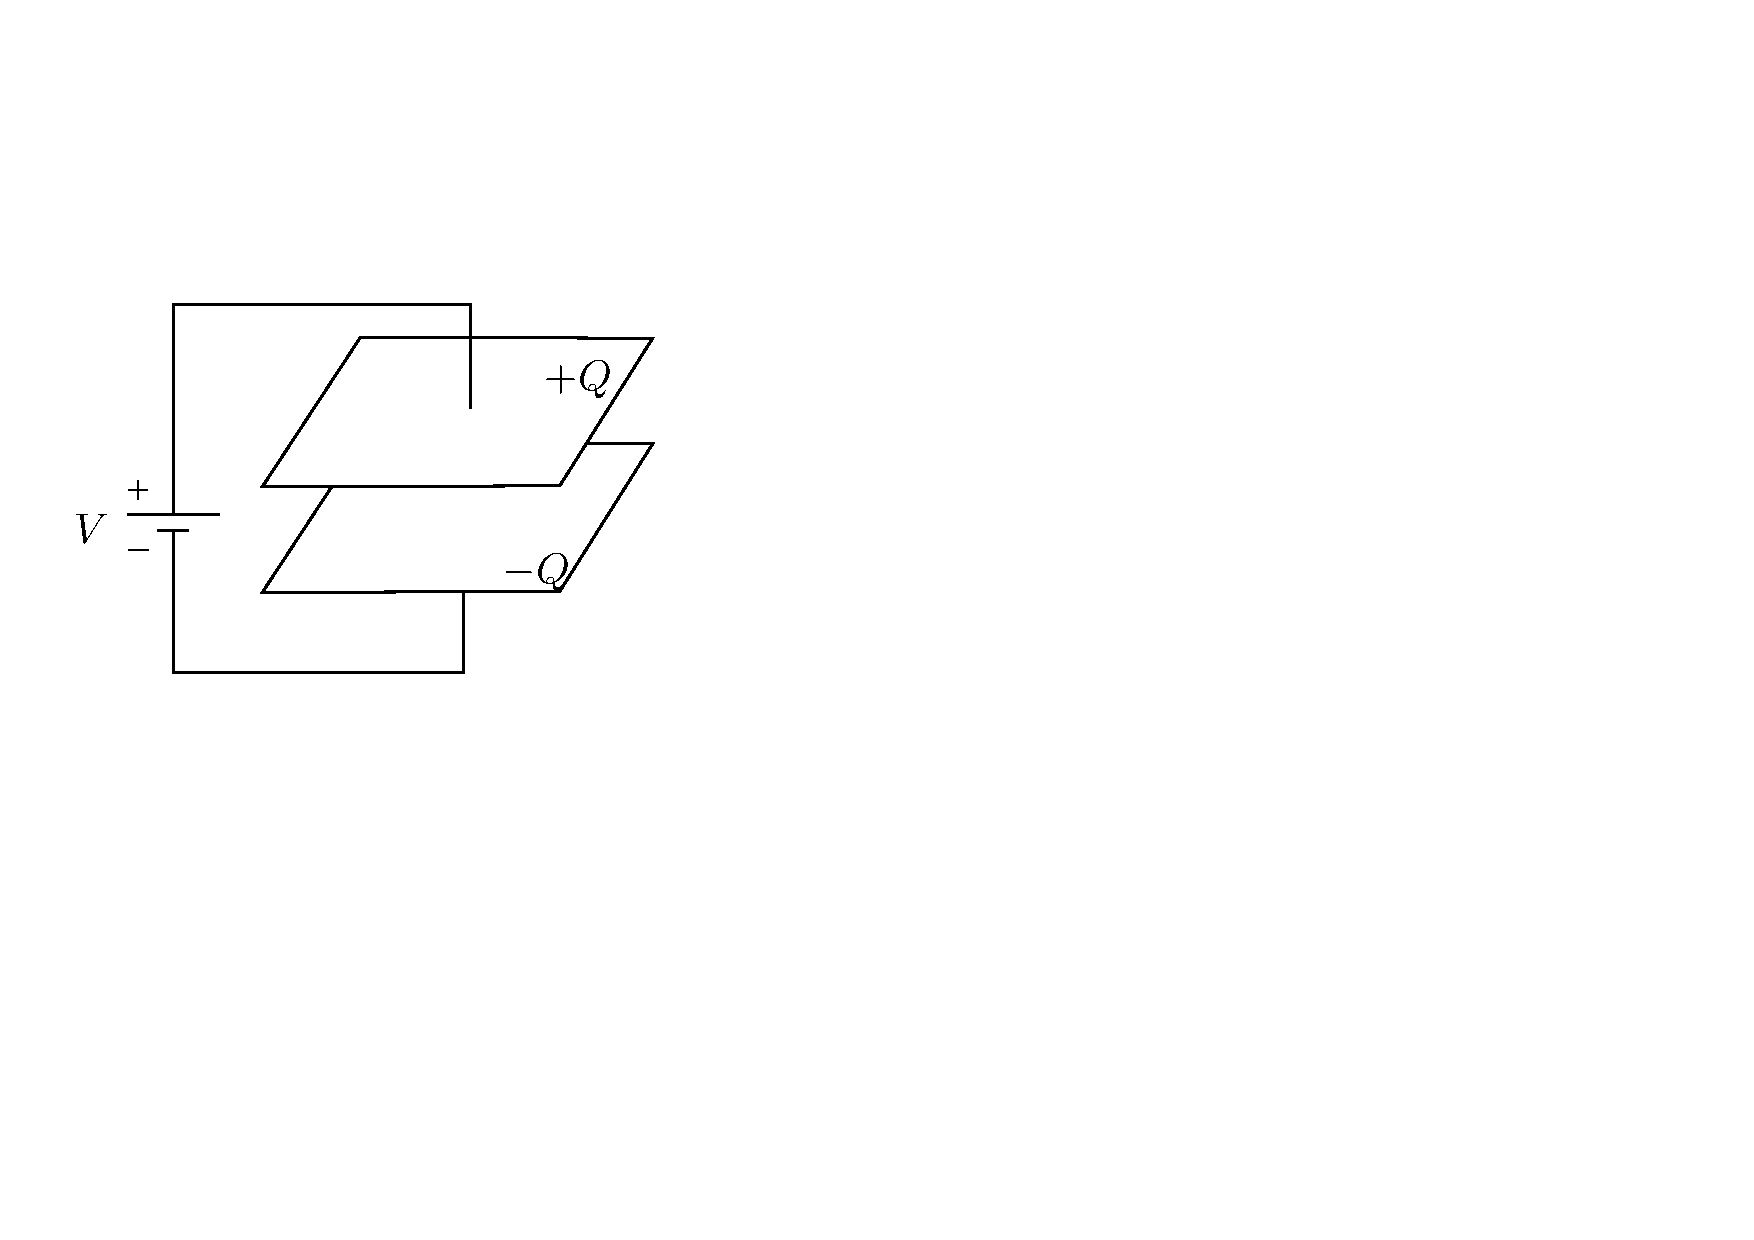
\includegraphics[width=4cm]{figs/figs_reg_trans/condensateur}
	\caption{Condensateur plan.} \label{fig:condensateur}
\end{marginfigure}
En pratique dans ce cours, nous allons toujours consid�rer la capacit� $C$ lin�aire et invariante, c'est-�-dire constante.
Comme le courant $i(t)$ est d�fini par 
$$i(t)=\frac{dq(t)}{dt}$$
on a 
$$i(t)=C\frac{du(t)}{dt}$$
ou encore 
$$ \quad u(t) = \frac{1}{C}\int_{-\infty}^t i(\tau) d\tau.$$
Ces relations sont �tablies selon le sens conventionnel (Figure~\ref{fig:capa_sens}).
\begin{marginfigure}
	\centering
	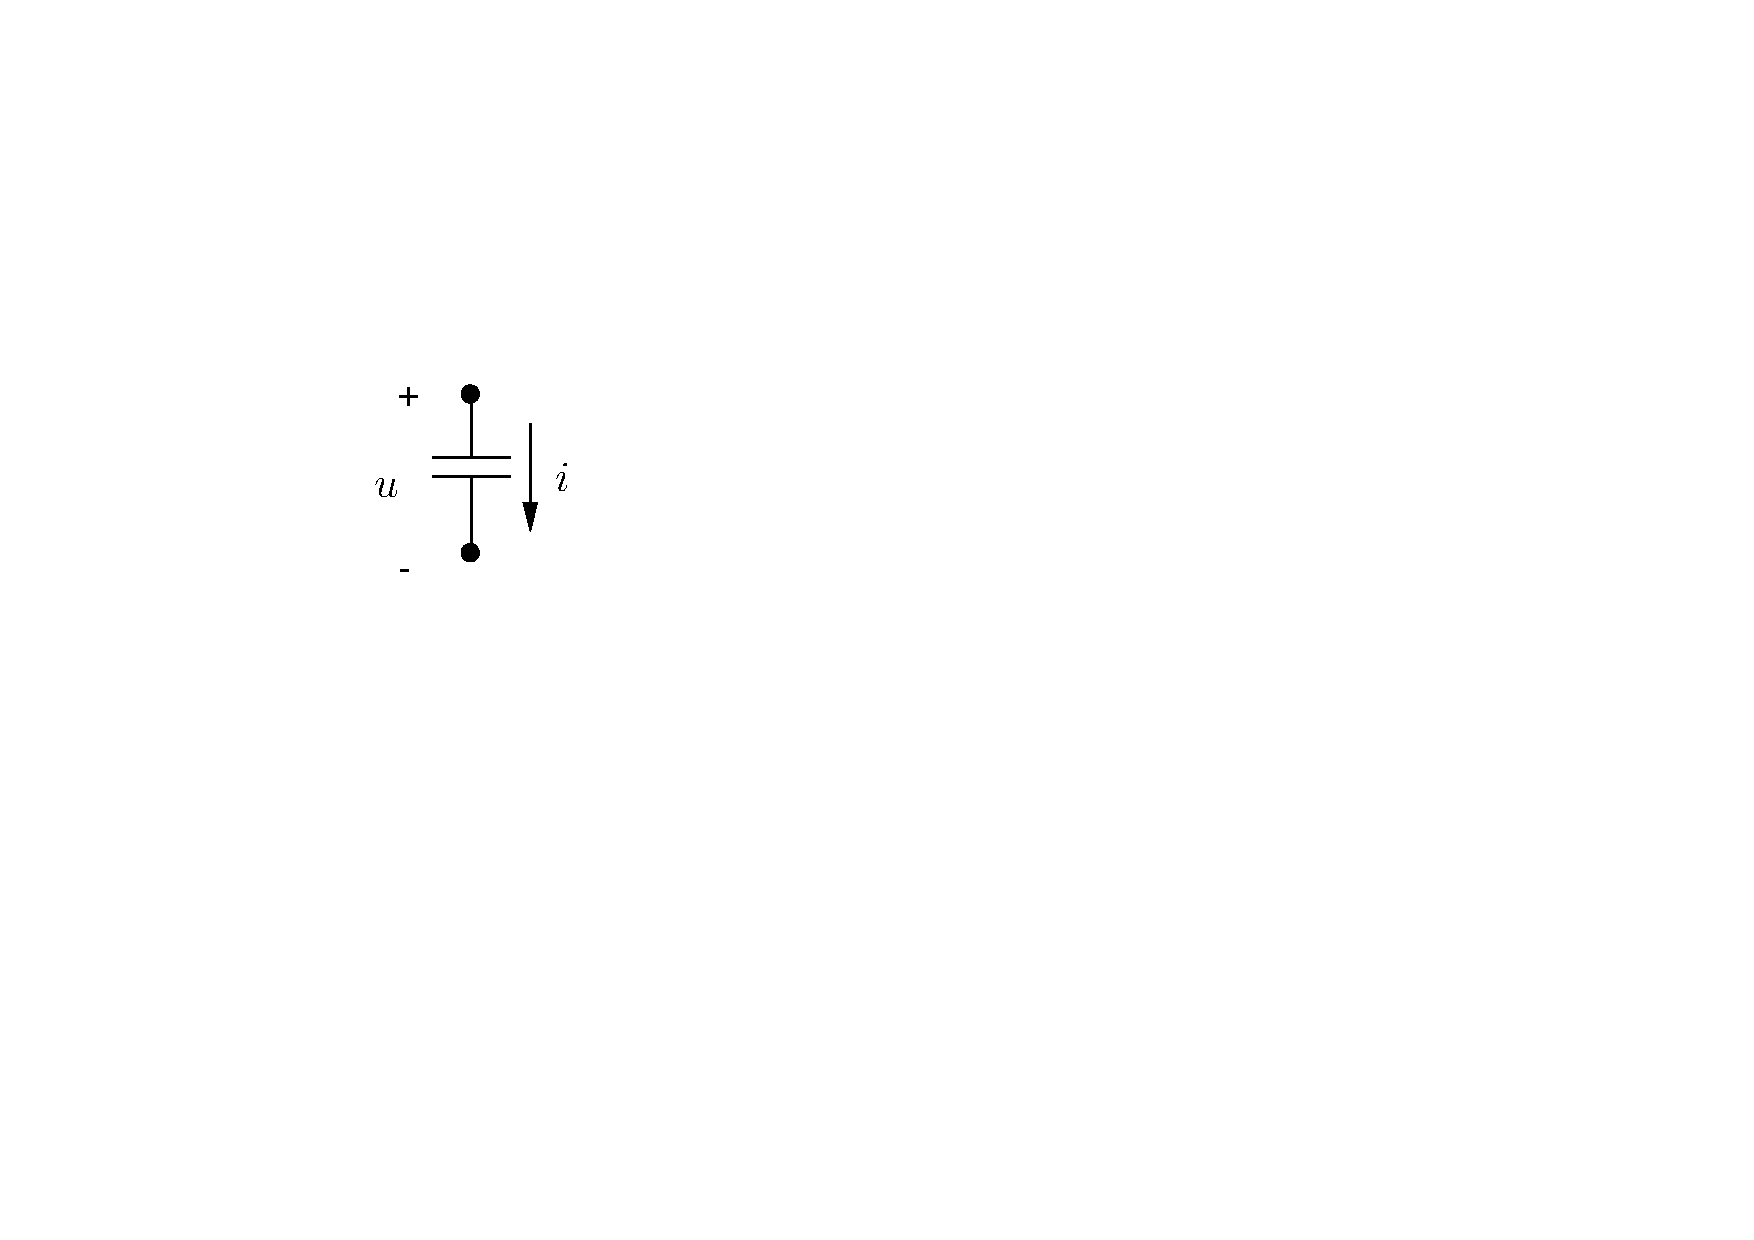
\includegraphics[width=2cm]{figs/figs_reg_trans/symbole_condensateur_et_sens.pdf}
	\caption{Symbole et sens conventionnel d'un condensateur.}\label{fig:capa_sens}
\end{marginfigure}
La propri�t� de lin�arit� d�pend des caract�ristiques du di�lectrique.

En toute g�n�ralit�, $C$ est fonction de la tension � ses bornes, du courant et peut varier avec le temps : 
$$C=f(u,i,t).$$
Si on consid�re le condensateur lin�aire mais temps variant, on a
$$ i(t)=C(t)\frac{du(t)}{dt} + \frac{dC(t)}{dt}u(t).$$
S'il est invariant mais fonction de la tension � ses bornes et du courant, on a $C=f(u,i)$ et 
$$ i(t)=C(u,i)\frac{du(t)}{dt}.$$
La relation entre $i(t)$ et $u(t)$ devient donc non-lin�aire.


La capacit� s'exprime, en fonction des param�tres physiques du condensateur par 
$$C=\frac{\epsilon S}{d}$$ o� $\epsilon$ est la permittivit� di�lectrique du mat�riau plac� entre les plaques, $S$ la surface des plaques, et $d$ la distance entre les plaques.
La capacit� s'exprime en farad ($F$).


\paragraph{En r�gime non stationnaire.}
Une variation du potentiel $V$ implique une modification de la charge
port�e par les plaques conductrices. Cette variation est apport�e par
un circuit ext�rieur d�bitant un courant.
Au niveau du condensateur :
\begin{itemize}
	\item la diff�rence de  potentiel � ses bornes varie
	\item le champ �lectrique $\overrightarrow{E}$ dans le mat�riau
	di�lectrique plac� entre les plaques est variable
	\item il existe un {\em courant de d�placement}.
	\[\vec{\nabla} \times \overrightarrow{H}  = 
	\frac{\partial \overrightarrow{D}}{\partial t}\]
\end{itemize}
Ce courant de d�placement et ce champ �lectrique variable sont
``confin�s'' � l'int�rieur de l'�l�ment, car on fait l'hypoth�se des circuits
localis�s.

Comme illustr� � la Figure~\ref{fig:capacitors}, il existe beaucoup d'impl�mentations physiques et chimiques de condensateur � di�lectrique � film plastique (polypropyl�ne, polyester, ...), c�ramique, au mica, �lectrolytique, � papier paraffin�, variable � lame d'air (une plaque mobile), etc. Habituellement, on indique la capacit� d'un condensateur en $pF$, $nF$ ou $\mu F$.
\begin{figure}[tb]
\centering
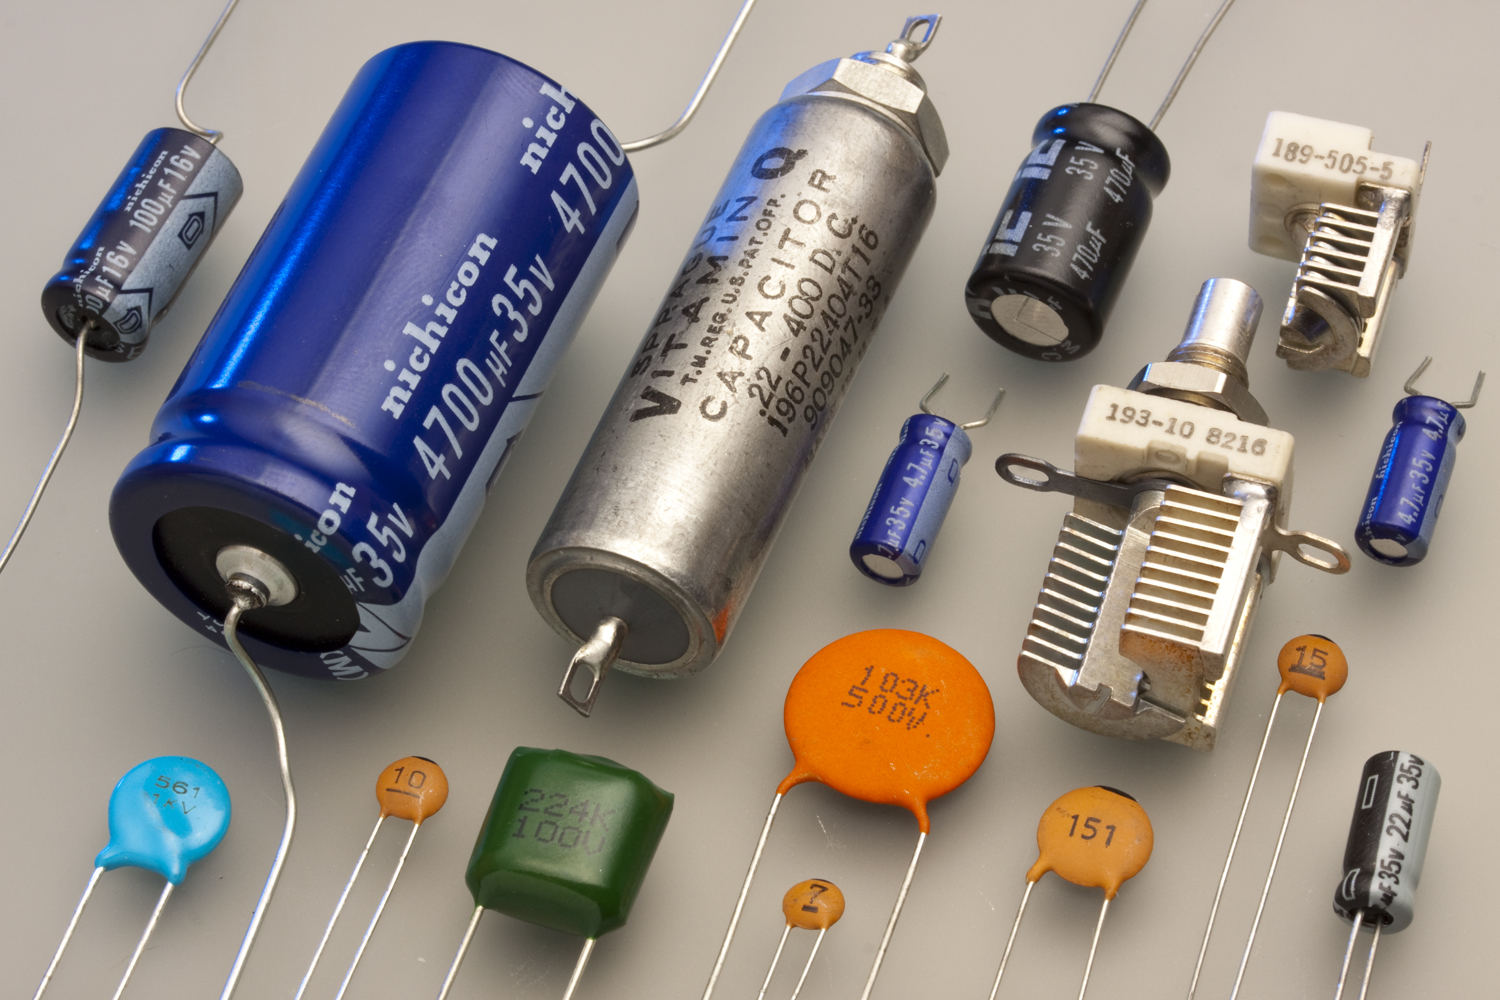
\includegraphics[width=0.98\linewidth]{figs/ch2_figs/capacitors}
\caption[Exemples des condensateurs.]{Exemples des condensateurs. Source: Wikipedia \url{https://fr.wikipedia.org/wiki/Condensateur}.\label{fig:capacitors}}
\end{figure}

\section{La diode}
\label{sec:diode}
Contrairement aux autres �l�ments passifs pr�sent�s, les r�sistances, condensateurs et bobines, une diode (Figure~\ref{fig:Diode}) est par essence un composant non-lin�aire. Une diode laisse passer le courant selon sa polarisation, i.e. le sens et l'amplitude de la tension � ses bornes. Lorsqu'une tension positive est appliqu�e entre l'anode et la cathode de la diode, le courant circule (de l'anode � la cathode). Si une tension n�gative est appliqu�e entre l'anode et la cathode, aucun courant ne circule\footnote{Sauf si cette tension inverse est d'amplitude assez importante, i.e. sup�rieure � la tension de claquage. Mais nous n'�tudierons pas ce cas d'utilisation dans ce cours.}.
\begin{marginfigure}[-8cm]
	\centering
	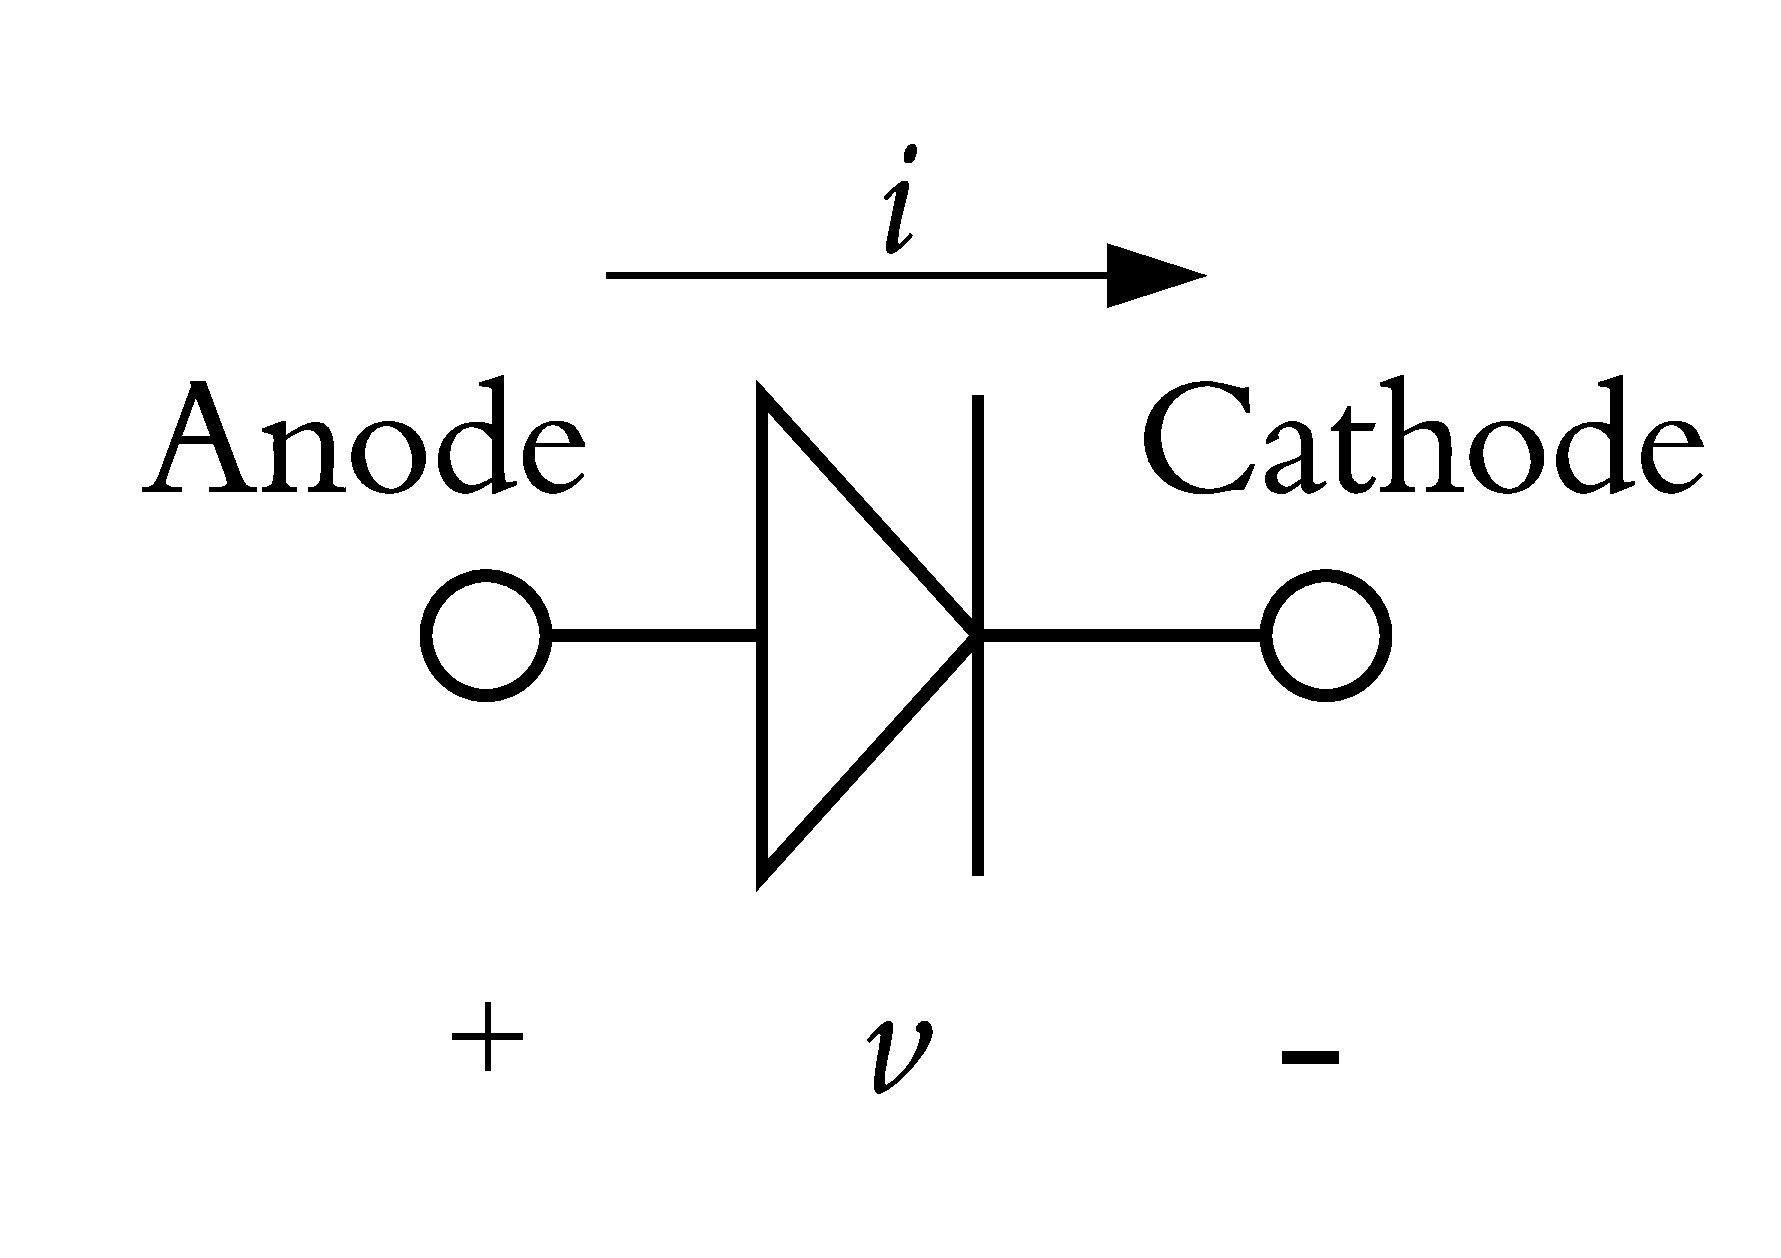
\includegraphics[width=0.7\linewidth]{figs/ch2_figs/Diode}
	\caption{Symbole d'une diode.}
	\label{fig:Diode}
\end{marginfigure}
La caract�ristique d'une diode id�ale est repr�sent�e � la Figure~\ref{fig:caracteristique_diode}. En pratique, selon les mat�riaux utilis�s, la tension de polarisation est sup�rieure � $0V$, et la courbe $i$-$u$ suit une exponentielle et est d�pendante de la temp�rature.
\begin{marginfigure}
\centering
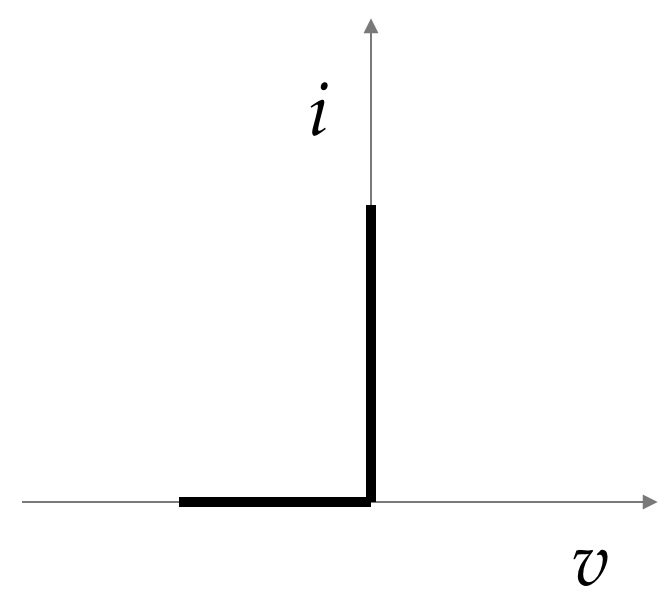
\includegraphics[width=0.7\linewidth]{figs/ch2_figs/caracteristique_diode}
\caption{Caract�ristique d'une diode id�ale.}
\label{fig:caracteristique_diode}
\end{marginfigure}


\section{Sources ind�pendantes d'�nergie}
\label{sec:sie}

Une source  ind�pendante d'�nergie est un composant capable de r�aliser une conversion d'�nergie de nature non �lectrique vers de l'�nergie �lectrique.
Par exemple, une batterie convertit de l'�nergie chimique, une dynamo de l'�nergie m�canique. Une centrale �lectrique convertit, selon sa source d'�nergie primaire, de l'�nergie nucl�aire, thermique ou solaire en �nergie m�canique puis en �nergie �lectrique. 

Les sources ind�pendantes d'�nergie sont en th�orie des circuits ce que les forces ext�rieures sont en m�canique. Deux sortes de sources ind�pendantes d'�nergie seront consid�r�es par la suite : sources de tension et sources de courant.

\paragraph{Source id�ale de tension.}
Une source id�ale de tension (Figure~\ref{fig:source_de_tension}) est un dip�le constitu� par un g�n�rateur de tension de force �lectromotrice $e(t)$. Elle a la propri�t� de pr�senter � ses bornes une d.d.p. ind�pendante du courant qui la parcourt. 


\begin{marginfigure}
	\centering
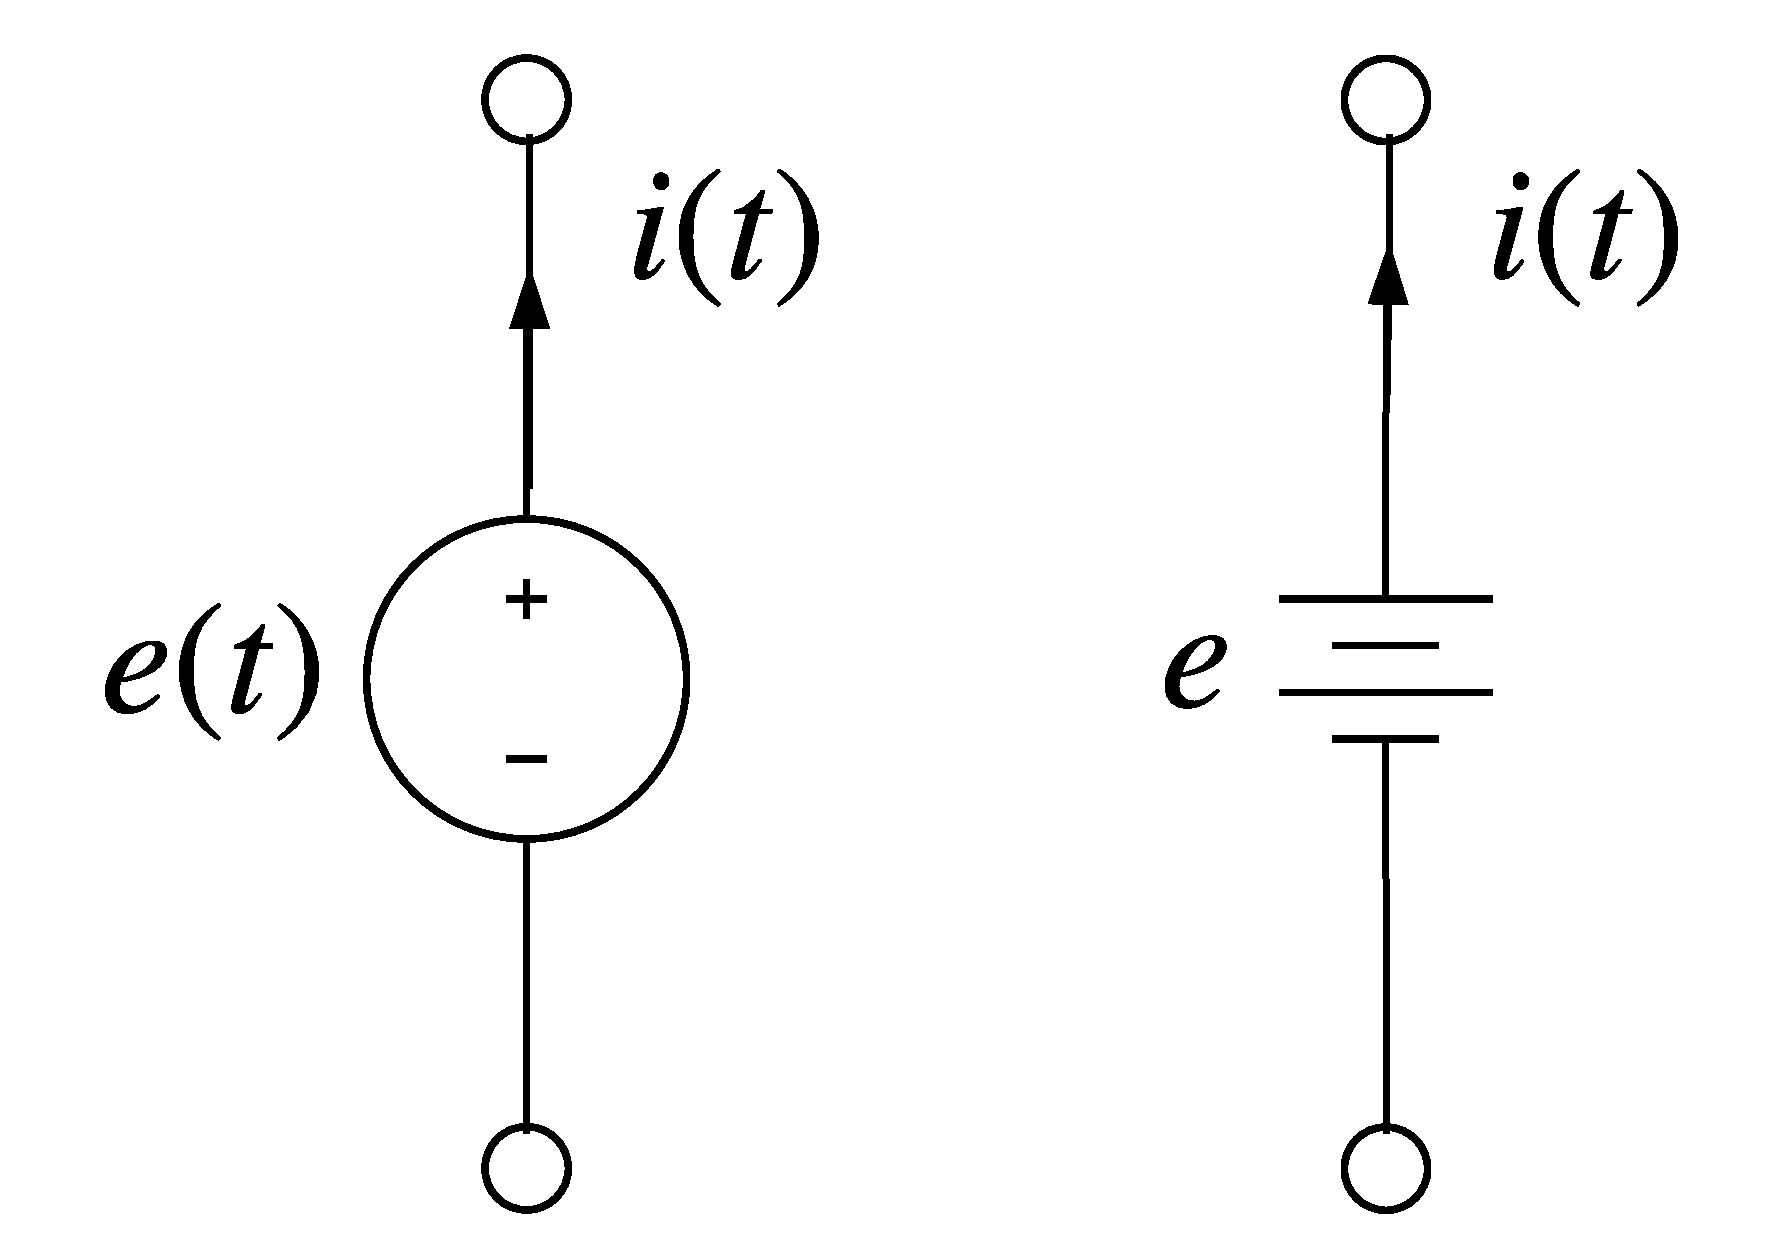
\includegraphics[width=0.9\linewidth]{figs/ch2_figs/sourceIndepV}
	\caption[Repr�sentations d'une source ind�pendante de tension.] {Repr�sentations d'une source ind�pendante de tension : g�n�rique (gauche) et continue (droite).}
	\label{fig:source_de_tension}
\end{marginfigure}

Les sens de r�f�rence associ�s sont indiqu�s sur la Figure~\ref{fig:source_de_tension} ; leur utilisation permet d'exprimer la puissance instantan�e fournie par la source quand elle est connect�e � un dip�le "charge" par le produit $e(t) i(t)$. Il s'agit ici d'une convention g�n�rateur, oppos�e � la convention moteur d�finie pr�c�demment.

Une source r�elle de tension poss�de rarement cette caract�ristique d'ind�pendance entre d.d.p. � ses bornes et courant, � cause de ses propres pertes. 
On peut rendre compte de ces pertes a l'aide d'une r�sistance interne $R_i$ et mod�liser la source r�elle de tension par une f.e.m. en s�rie avec $R_i$. La Figure~\ref{fig:source_de_tension_reelle} repr�sente une source r�elle de tension continue ; elle indique que lorsque ce dip�le est ferm� sur une r�sistance ext�rieure de charge\footnote{On utilise souvent l'indice $L$ pour nommer la r�sistance qui \textit{charge} le circuit, car le terme \textit{charge} se traduit par \textit{load} en anglais.} $R_L$, il pr�sente une d.d.p. fonction du courant :
$$U= E -R_i I.$$
\begin{marginfigure}
	\centering
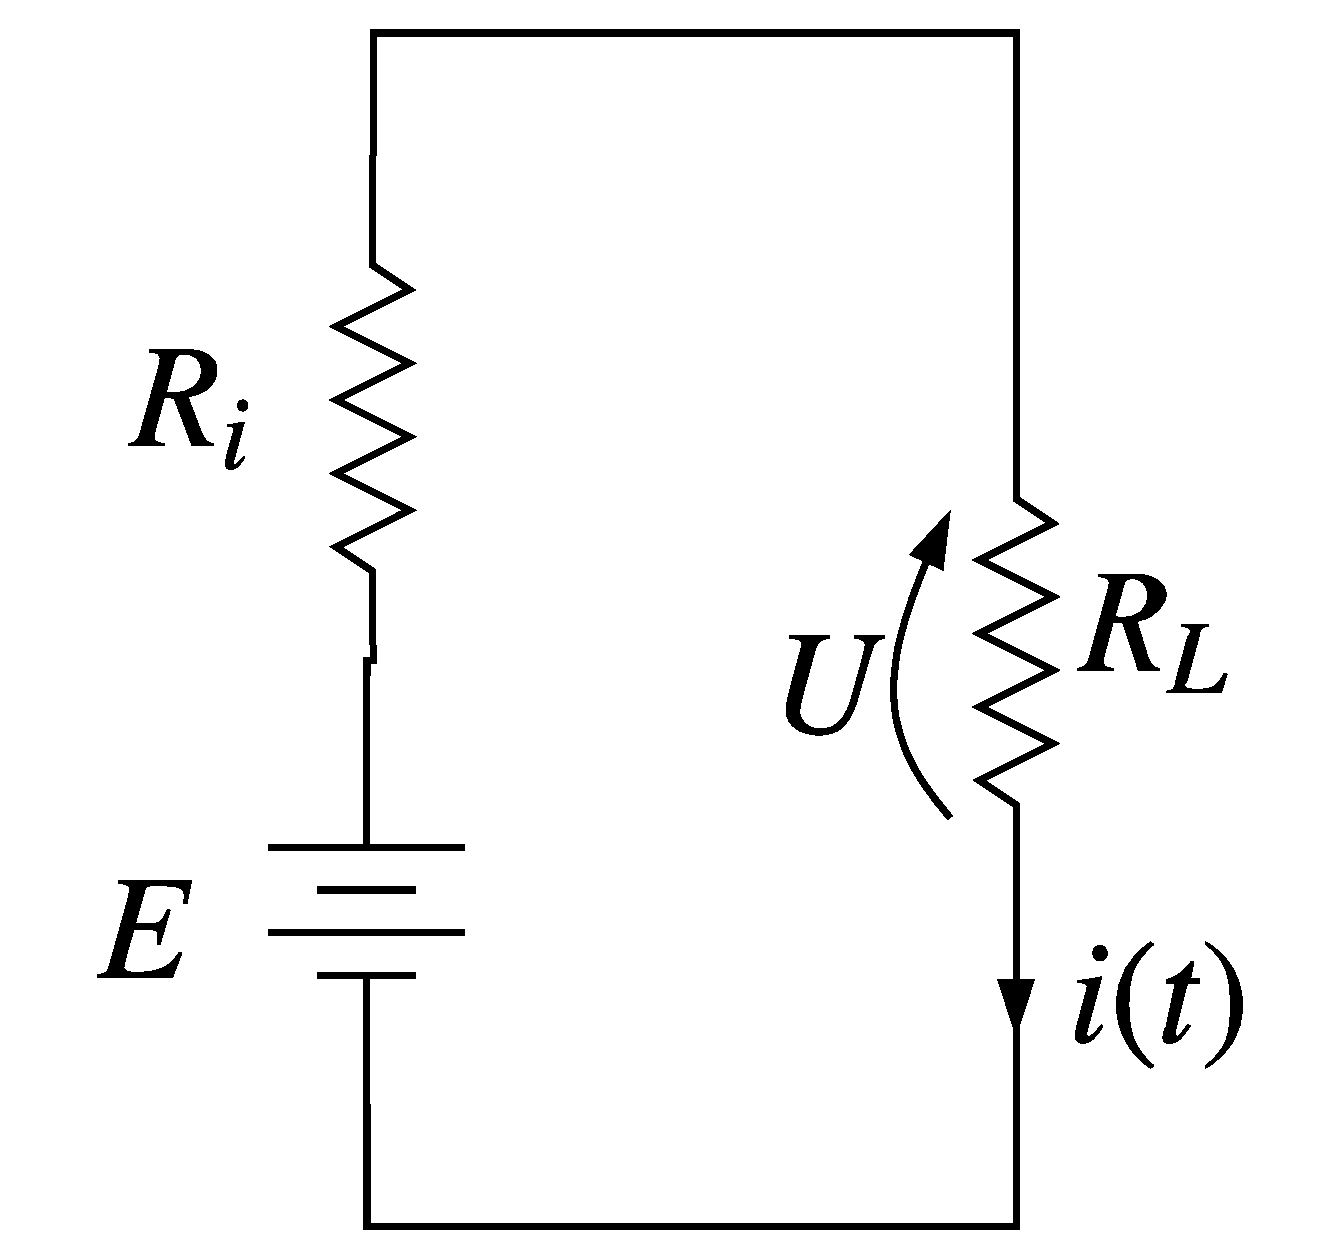
\includegraphics[width=0.7\linewidth]{figs/ch2_figs/SourceReelleV}
	\caption[Source ind�pendante de tension r�elle] {Repr�sentation d'une source ind�pendante de tension r�elle.}
	\label{fig:source_de_tension_reelle}
\end{marginfigure}
La condition sous laquelle cette source r�elle se rapproche de la source id�ale se d�duit � partir de :
$$U=R_L I = R_L \frac{E}{R_L+R_i} = \frac{E}{1+R_i/R_L}.$$
Donc $U \approx E$ si $R_L \gg R_i$. 

Notons que la puissance fournie par la source de tension � $R_L$ vaut
$$UI=R_L \frac{E^2}{{(R_L+R_i)}^2}.$$

La Figure~\ref{fig:source_de_tension_reelle} met en �vidence un formule d'utilit� pratique tr�s fr�quente lorsqu'on souhaite calculer la tension aux bornes d'une r�sistance en s�rie avec une autre. Ce circuit agit comme un \textit{diviseur de tension} : 
\begin{table}[h]
	\caption{Formule du diviseur de tension.}
	\begin{boxedminipage}{\linewidth}
		$$ U = E \frac{R_L}{R_L+R_i}.$$
	\end{boxedminipage}
\end{table}


\paragraph{Source id�ale de courant.}
Une source id�ale de courant est un dip�le constitu� par un injecteur de courant $j(t)$. 
Elle a la propri�t� de fournir une intensit� de courant ind�pendante de la d.d.p. � ses bornes. 
La Figure~\ref{fig:source_de_courant} repr�sente une telle source de courant ainsi que le sens conventionnel associ�. 
\begin{marginfigure}
	\centering
	\begin{circuitikz}
		\draw (0, 0)  to [american current source, l=$j(t)$, v>=$e(t)$, o-o] ++(0,2.5) ;
	\end{circuitikz}
	\caption[Repr�sentations d'une source ind�pendante de tension.] {Repr�sentations d'une source ind�pendante de courant.}
	\label{fig:source_de_courant}
\end{marginfigure}
De nouveau, le produit $j(t) e(t)$ repr�sente, avec ce sens, la
puissance fournie par la source, lorsque celle-ci est connect�e � un "dip�le de charge".

Une source r�elle de courant poss�de rarement cette caract�ristique d'ind�pendance entre courant et d.d.p. � ses bornes. On la mod�lise usuellement par une source id�ale de courant en parall�le avec sa conductance interne. La Figure~\ref{fig:source_courant} repr�sente une source r�elle de courant, aux bornes de laquelle est connect�e une "conductance de charge" $G_L$. On v�rifie ais�ment que cette source r�elle se rapproche de la source id�ale lorsque $G_i \ll G_L$. En effet,
$$i=G_L u = G_L \frac{J}{G_L+G_i} = \frac{J}{1+G_i/G_L}.$$
\begin{marginfigure}[-2cm]
\centering
\includegraphics[width=0.98\linewidth]{figs/ch2_figs/sourceDeCourantReelle}
\caption{Source r�elle de courant.}
\label{fig:source_courant}
\end{marginfigure}

Chaque type de source peut fournir un signal dont l'�volution temporelle est quelconque. Le plus souvent, il sera continu (i.e. constant) ou sinuso�dal.


La Figure~\ref{fig:source_courant} permet �galement de mettre en �vidence un formule d'utilit� pratique tr�s fr�quente lorsqu'on souhaite calculer le courant dans une branche d'un dip�le constitu� de la mise en parall�le de plusieurs r�sistances. Ce circuit agit comme un \textit{diviseur de courant} : 
\begin{table}[h]
\caption{Formule du diviseur de courant.}
\begin{boxedminipage}{\linewidth}
$$ i = J \frac{G_L}{G_L+G_i}.$$
\end{boxedminipage}
\end{table}

\section{Les sources d�pendantes de courant et de tension}
Une source command�e est un quadrip�le unidirectionnel, non-autonome et actif ; un
de ses acc�s est celui qui exerce la commande (acc�s de commande), l'autre est l'acc�s command�. Autrement dit, la tension ou le courant d�livr� par la source d�pend de la valeur d'une d.d.p. ou d'un courant � un autre endroit du circuit.

On distingue les quatre types de sources command�es id�ales illustr�es � la Figure~\ref{fig:VVT}.
\begin{figure}[tb]
	\centering
	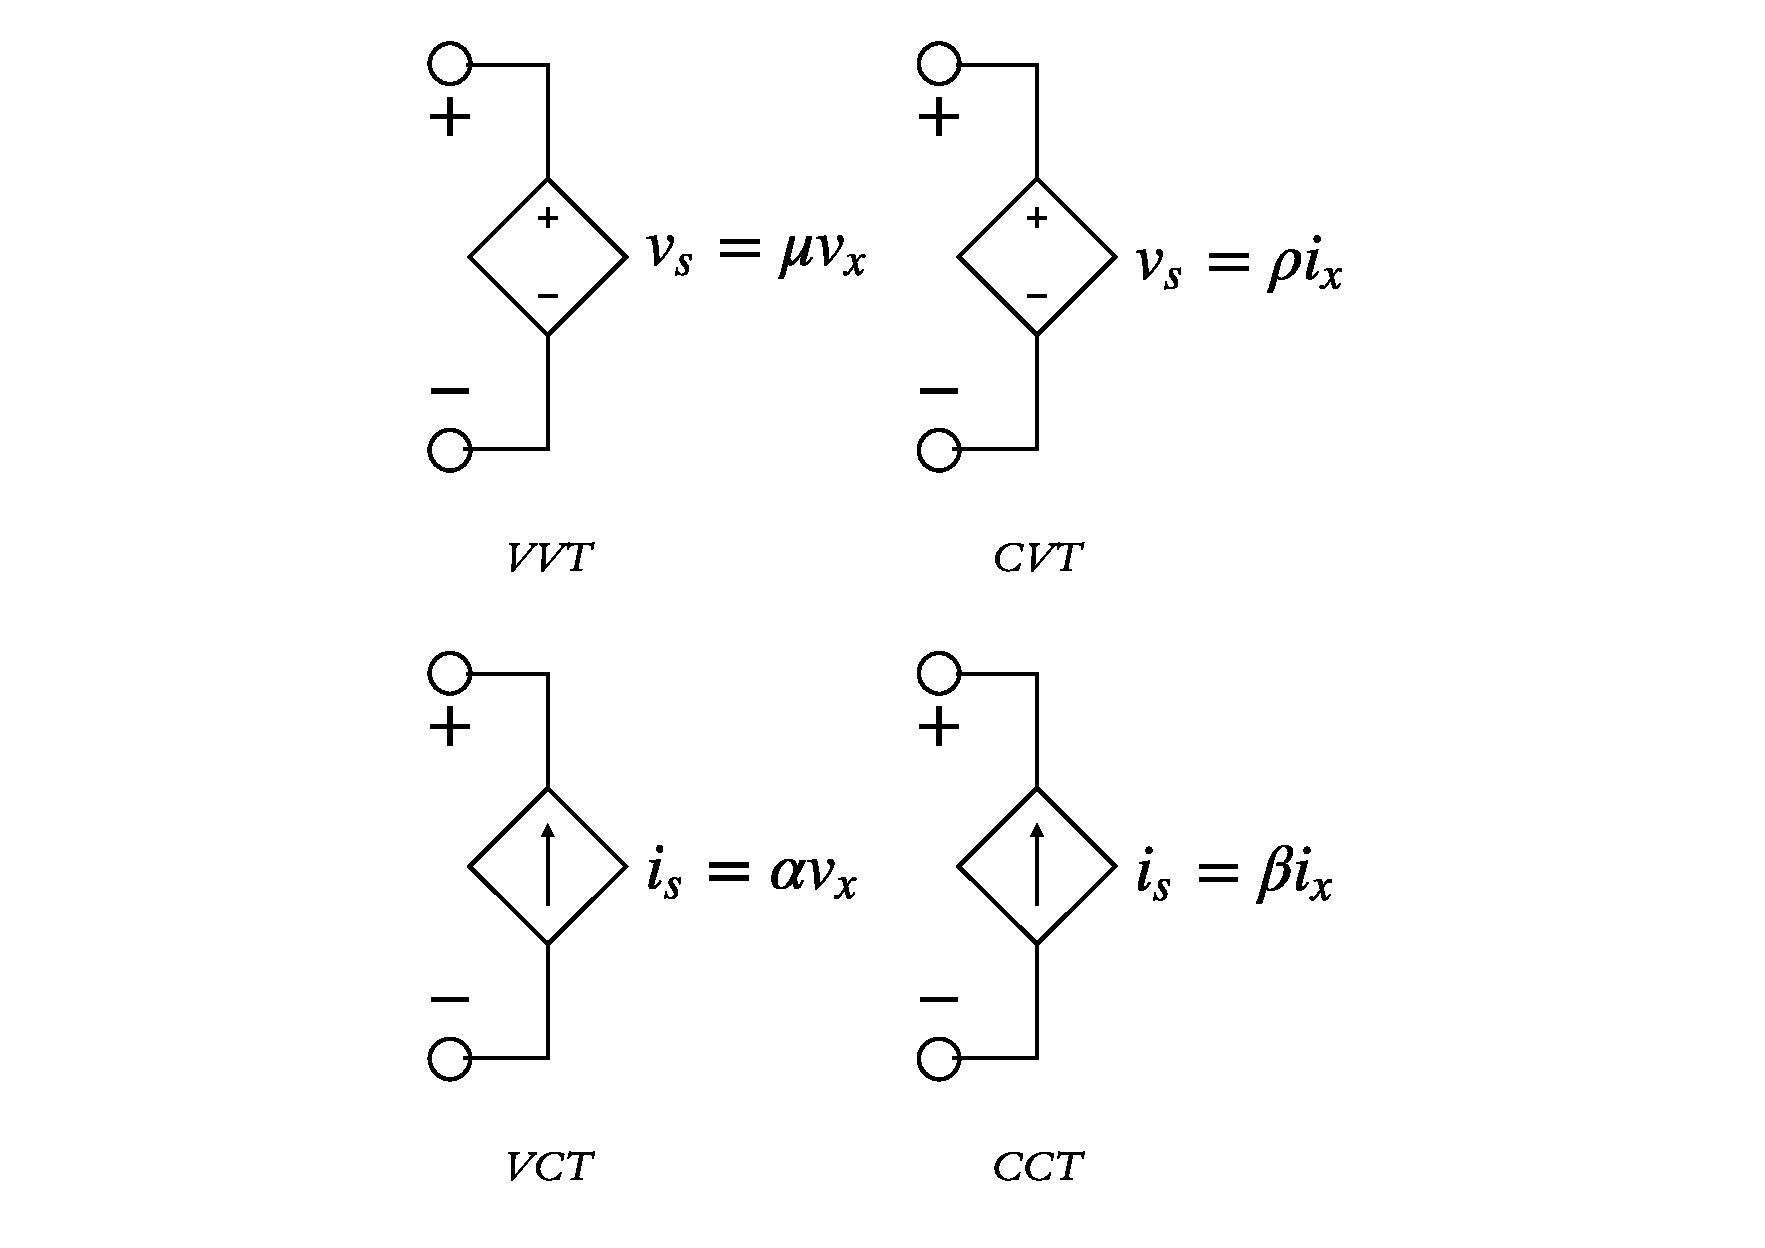
\includegraphics[width=\linewidth]{figs/ch2_figs/SourcesCommandees}
	\caption{Source command�es : tension-tension, courant-tension $[\rho] = \frac{[V]}{[I]}=[\Omega]$, tension-courant $[\alpha] = \frac{[I]}{[V]}=[S]$, courant-courant.}
	\label{fig:VVT}
\end{figure}
Pour une source command�e tension-tension (VVT : voltage to voltage transducer), 
$v_s$ n'est d�termin� � l'instant $t$ que si la valeur $v_x(t)$ est connue.
$v_x$ est la tension de commande et $v_s$ la tension command�e.
Le coefficient multiplicatif $\mu$ ($\neq 0$) est sans dimension.
De mani�re similaire, les trois autres combinaisons sont courant-tension (CVT), tension-courant (VCT) et  courant-courant (CCT).

Puisque les relations de d�pendance introduites ci-dessus sont lin�aires, ces sources command�es sont des �l�ments lin�aires. Les sources d�pendantes ne sont pas des excitations. 
Elles sont analogues � des �l�ments r�sistifs et introduisent un couplage entre
diff�rentes branches du circuit.
Comme nous le verrons au Chapitre~\ref{cha:AO}, les sources command�es sont utiles pour la mod�lisation de circuits �lectroniques.



\section{Passivit� des �l�ments $R$, $L$ et $C$ lin�aires et invariants}

La puissance \textbf{absorb�e} par une r�sistance lin�aire est,
en utilisant la \textbf{convention moteur} (Figure~\ref{fig:conv_r}) : 
\begin{eqnarray*}
p_R(t)&  =& u(t)i(t) \\ 
& =& Ri(t)i(t) = Ri^2(t) \geq 0,
\end{eqnarray*}
et en utilisant la \textbf{convention g�n�rateur}:
\begin{eqnarray*}
p_R(t)&  =& -u(t)i(t) \\
& =& Ri(t)i(t) = Ri^2(t) \geq 0.
\end{eqnarray*}
\begin{marginfigure}%[-3cm]
	\begin{center}
		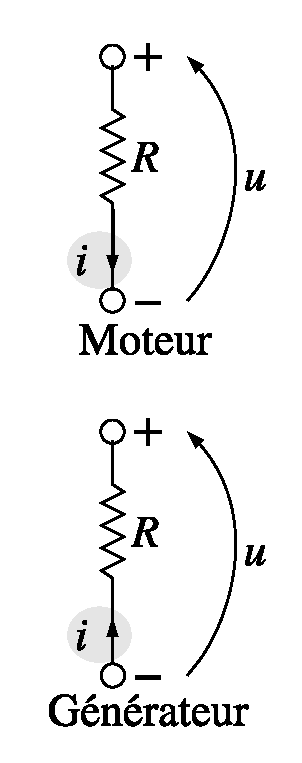
\includegraphics[width=0.5\linewidth]{figs/ch2_figs/convention_moteur}
	\end{center}
\caption{Conventions moteur et g�n�rateur pour un dip�le r�sistif. \label{fig:conv_r}}
\end{marginfigure}
L'�nergie dissip�e vaut  \[w_R(t)=\int_{-\infty}^t
p(\tau)\, d\tau > 0.\]
Une \textbf{r�sistance} $R$ est donc un �l�ment \textbf{passif} car $w_R(t)>0$, et \textbf{dissipatif} car $p_R(t) \geq 0 $.

Pour des bobines ($L$) et des condensateurs ($C$) lin�aires on a (avec la convention moteur) : 
\begin{center}
\begin{tikzpicture}[y=-1cm]
\sf
\filldraw[black] (7.6,2.1) circle (0.06667cm);
\filldraw[black] (7.6,3.66667) circle (0.06667cm);
\draw[arrows=-triangle 45,black] (8.04444,2.33333) -- (8.04444,3.51111);
\path (7.27778,2.15556) node[text=black,anchor=base east] {+};
\path (7.34444,3.77778) node[text=black,anchor=base east] {-};
\path (7.15556,3.08889) node[text=black,anchor=base east] {$u$};
\path (8.16667,3.05556) node[text=black,anchor=base west] {$i$};
\filldraw[black] (1.84222,2.25111) circle (0.06667cm);
\filldraw[black] (1.84222,3.54667) circle (0.06667cm);
\draw[arrows=-triangle 45,black] (2.33333,2.48889) -- (2.33333,3.37778);
\path (1.42222,2.34444) node[text=black,anchor=base east] {+};
\path (1.35556,3.76667) node[text=black,anchor=base east] {-};
\path (1.25556,3.08889) node[text=black,anchor=base east] {$u$};
\path (2.53333,3.04444) node[text=black,anchor=base west] {$i$};
\draw (7.62,2.49333) +(-97:0.16566) arc (-97:134:0.16566);
\draw (7.61333,2.75111) +(-127:0.17601) arc (-127:128:0.17601);
\draw (7.61333,3.02889) +(-127:0.17601) arc (-127:128:0.17601);
\draw (7.62,3.28444) +(97:0.16345) arc (97:-134:0.16345);
\draw (7.6,2.14444) -- (7.6,2.32889);
\draw (7.6,3.44667) -- cycle;
\draw (7.6,3.44667) -- (7.6,3.63333);
\draw (1.53333,2.76667) -- (2.16889,2.76667);
\draw (1.85111,2.28889) -- (1.85111,2.76667);
\draw (1.85111,2.92444) -- (1.85111,3.56);
\draw (1.53333,2.92222) -- (2.16889,2.92222);

\end{tikzpicture}%

%% Configure (x)emacs for this file ...
%% Local Variables:
%% mode: latex
%% End:
\end{center}
\begin{minipage}[c]{6cm}
\begin{align*}
p_C(t) & =Cu(t)\frac{du(t)}{dt} \gtreqless 0\\[3mm]
w_C(t) & =\int_{-\infty}^t
Cu(t)\frac{du(t)}{dt} \\[3mm]
& = \frac{1}{2}C\,u^2(t) \geq 0
\end{align*}
\end{minipage}
\begin{minipage}[c]{6cm}
\begin{align*}
p_L(t)&=Li(t)\frac{di(t)}{dt} \gtreqless 0\\[3mm]
w_L(t) & =\int_{-\infty}^t
Li(t)\frac{di(t)}{dt}\\[3mm]
& = \frac{1}{2}L\,i^2(t) \geq 0
\end{align*}
\end{minipage}
$L$ et $C$ sont donc des �l�ments \textbf{passifs} ($w(t) \geq 0$), mais \textbf{non dissipatifs},
ils restituent de la puissance quand $p(t) < 0$.

On peut donc au final classer les �l�ments comme indiqu� � la Figure~\ref{fig:classification}.
\begin{figure}
	\centering
	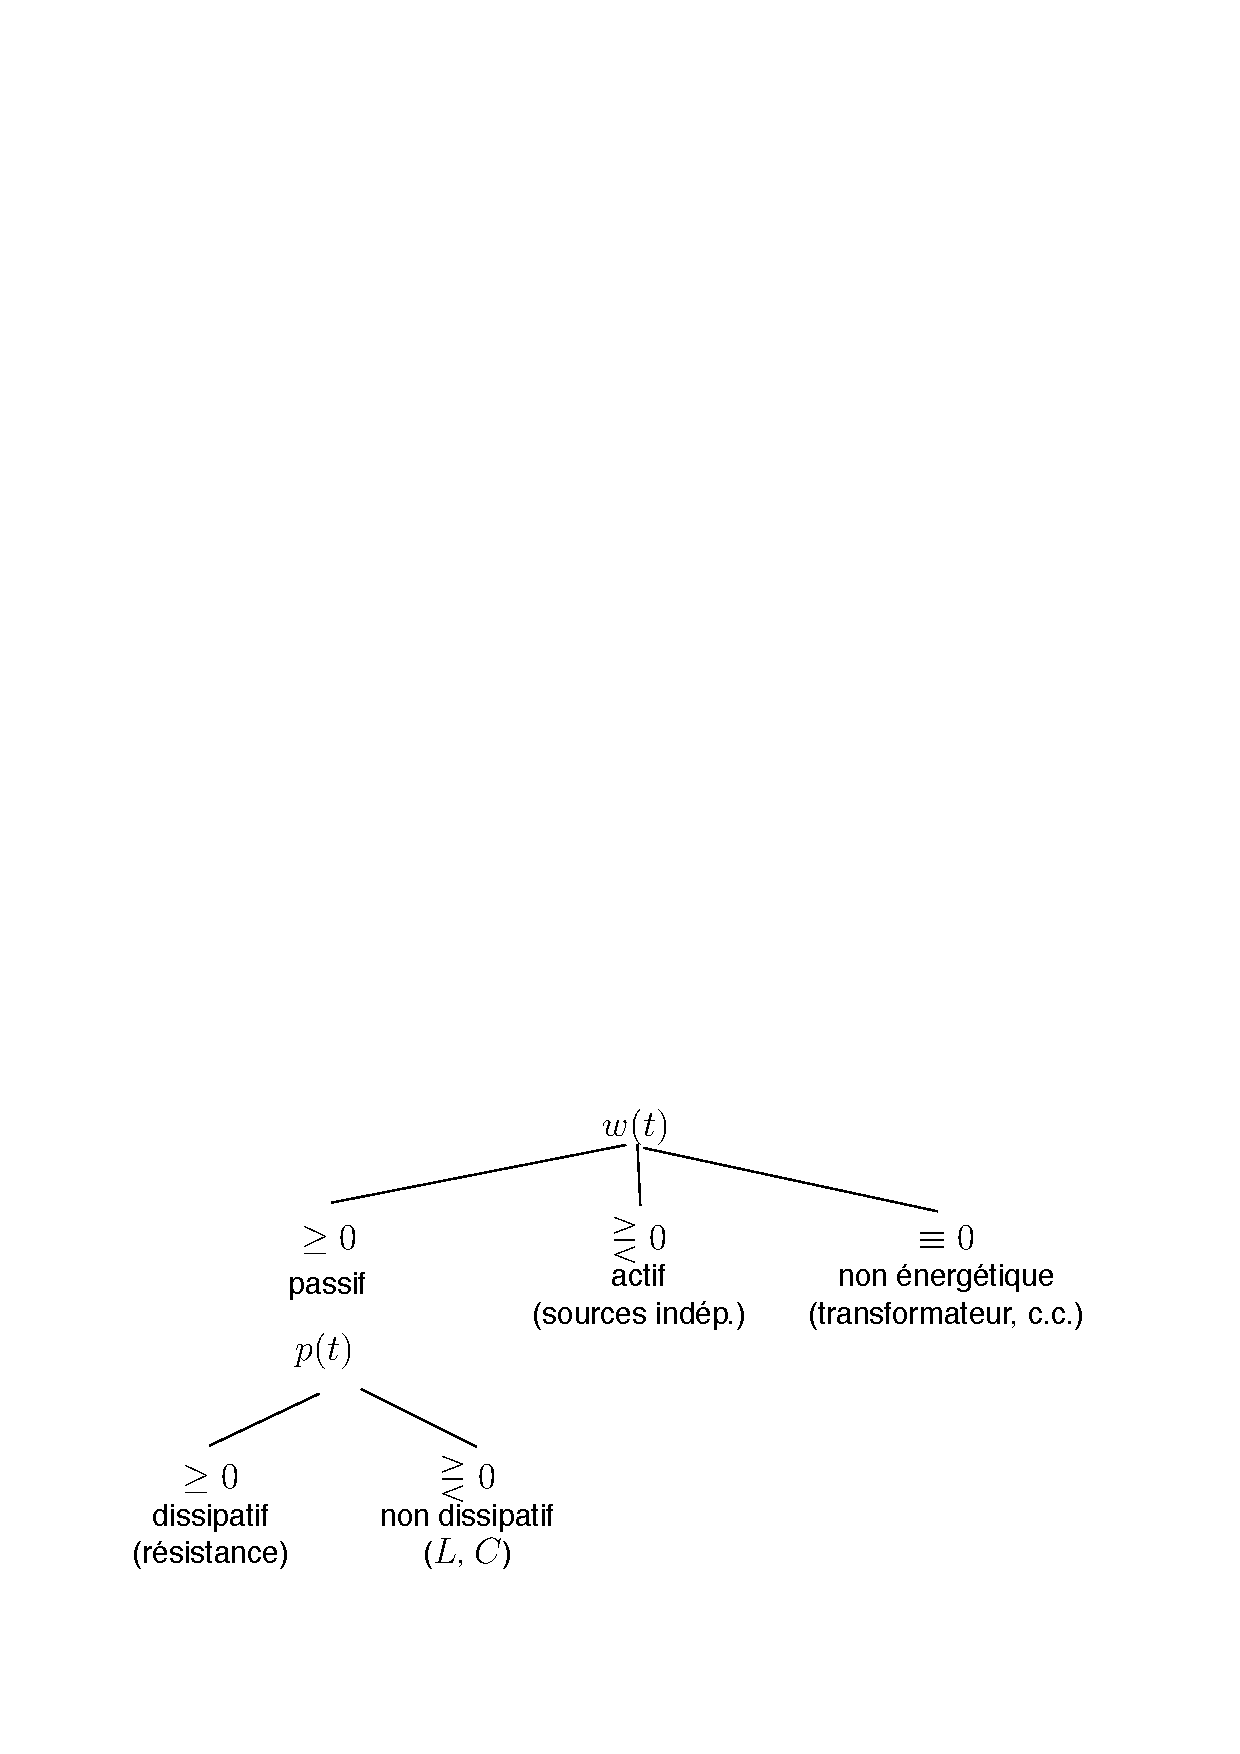
\includegraphics{figs/ch2_figs/puissclassi.pdf}
	\caption{Classification �nerg�tique des �l�ments.}
	\label{fig:classification}
\end{figure}

\section{Sch�ma d�taill� de la radio AM}
La Figure~\ref{fig:RadioAM_diode} repr�sente un sch�ma d�taill� de la radio AM introduite dans la Section~\ref{sec:pratique}. Il est important de remarquer que si deux arr�tes se croisent � l'ext�rieur des �l�ments sans qu'il n'y ait de \tikzcircle{2pt} � leur intersection, alors il n'y a aucun contact �lectrique entre les "fils" correspondants. On omet cependant parfois le \tikzcircle{2pt} lorsque deux arr�tes forment un \textsf{T}.
\begin{figure*}[p]
	\centering
	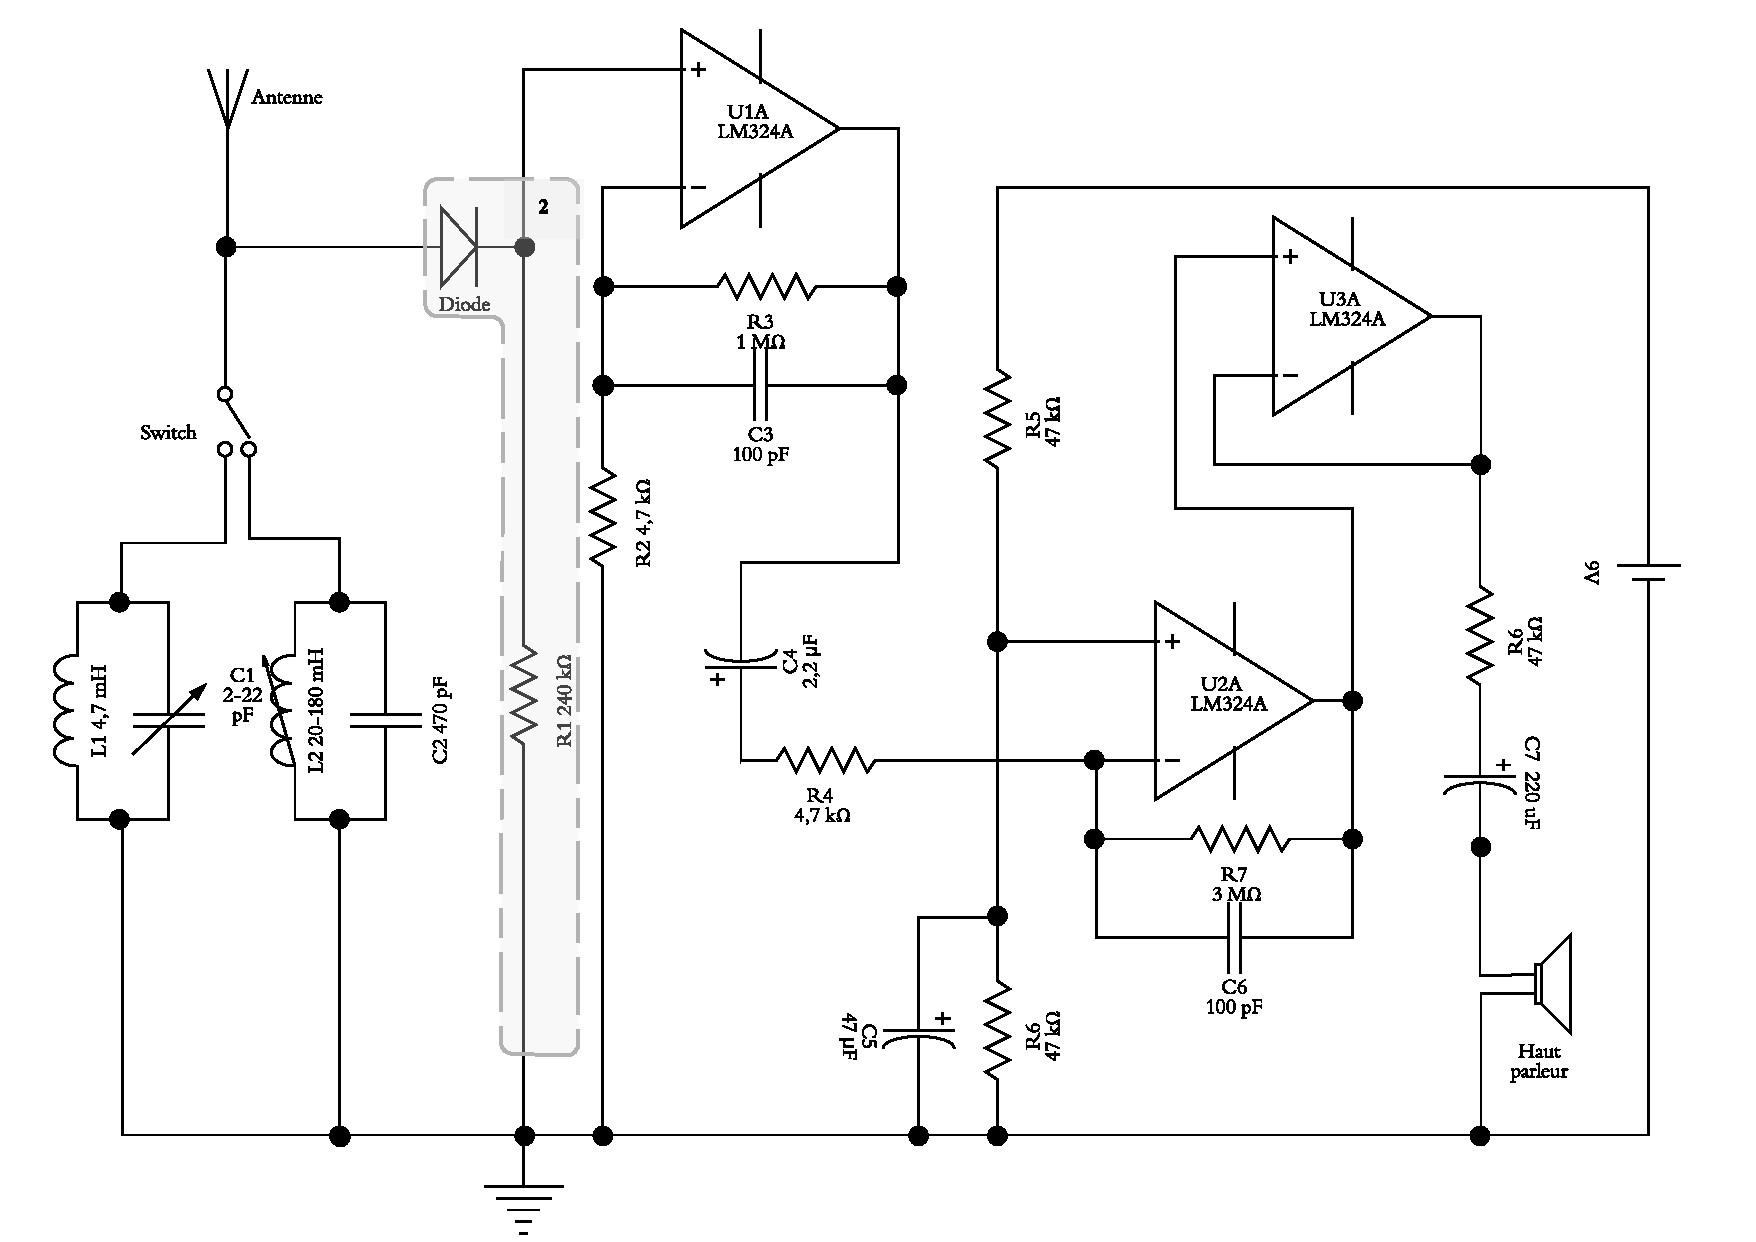
\includegraphics[angle=90, origin=c, scale=1.4]{figs/RadioAM/RadioAM_rect_1}
	\caption{Coupe 2: premi�re partie du circuit redresseur.}
	\label{fig:RadioAM_diode}
\end{figure*}
Le graphe comporte $n=12$ noeuds, plusieurs r�sistances, plusieurs condensateurs (simples et �lectrolytiques) et deux bobines. Le switch permet de s�lectionner soit le circuit LC o� C est variable ($L1$, $C1$), soit le circuit LC o� L est variable ($L2$, $C2$).

En pratique, l'analyse de ce circuit ne se fait pas d'un bloc. Le circuit est d�compos� en plusieurs �tages, qui sont analys�s dans les chapitres suivants.

\subsection{D�modulation de la radio AM}
� ce stade, un seul �tage peut �tre analys� : la premi�re partie de la d�modulation illustr�e par la coupe $2$ de la Figure~\ref{fig:RadioAM_diode}. 
En supposant que le signal d�sir� est re�u (ce qui sera expliqu� dans le Chapitre~\ref{cha:filtres}), il faut le d�moduler pour l'utiliser. Bien que le r�cepteur � cristal soit extr�mement simple, il est l'�l�ment le plus important du circuit.
C'est la diode qui va extraire la modulation, c'est-�-dire le signal audio (signal modulant, voir Figure~\ref{fig:mod2}), du signal radio. La d�modulation consiste � d�tecter l'enveloppe du signal modul�. 
\begin{figure}[h!]
  	\centering
  	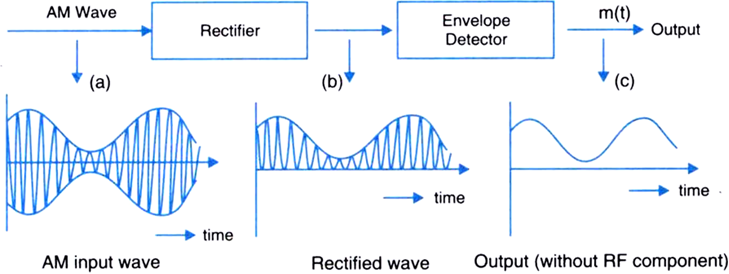
\includegraphics[width=10cm]{figs/RadioAM/demod.png}
  	\caption{Principe de la d�modulation d'un signal radio}
  	\label{fig:demod}
\end{figure}
La Figure~\ref{fig:demod} nous montre que la d�modulation s'effectue en deux �tapes:
\begin{enumerate}
  	\item le redressement du signal \textit{(Rectifier)},
  	\item la d�tection de l'enveloppe \textit{(Envelope Detector)}.
\end{enumerate}
La diode s'occupe par d�finition de l'�tape 1 (Figure~\ref{fig:RadioAM_diode}). Les alternances positives d'un signal sont transmises, tandis que les n�gatives sont bloqu�es. Le signal est donc \textit{redress�}. La r�sistance $R1$, bien que de valeur relativement �lev�e, offre un chemin pour le courant. En effet, nous verrons que la r�sistance d'entr�e de l'amplificateur op�rationnel $U1A$ est tr�s grande (Chapitre~\ref{cha:AO}).


% !TeX root = syllabus_ELEC0053.tex
% !TeX encoding = ISO-8859-1
% !TeX spellcheck = fr_FR

\section{Exercices}

\begin{exwithsol}{Bilan de puissance.}{solex:1-1}
\label{ex:1-1}
%\paragraph{Exercice 1.1 - Bilan de puissance.}
\noindent D�terminer le bilan de puissance pour chacun des 3 circuits ci-dessous.
\begin{center}
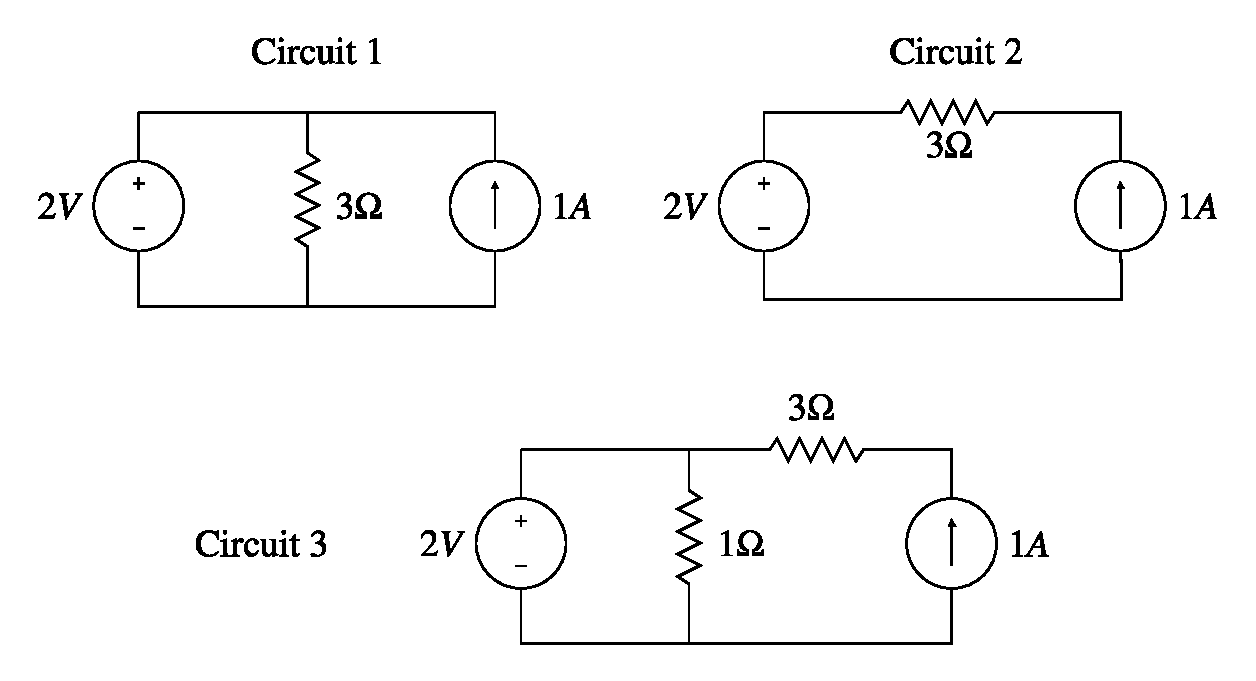
\includegraphics{exercices/ex-1-1}
\end{center}
\rep{Circuit 1: $p_R=\frac{4}{3}$ W, $p_J=2$ W, $p_E=-\frac{2}{3}$ W \\
Circuit 2: $p_R=3$ W, $p_J=5$ W, $p_E=-2$ W \\ 
Circuit 3: $p_{1\Omega}=4$ W, $p_{3\Omega}=3$ W, $p_E=2$ W, $p_J=5$ W}
\end{exwithsol}

\begin{exwithsol}{Lois de Kirchhoff et loi d'Ohm.}{solex:1-2}
\label{ex:1-2}
D�terminer le courant $I_0$ d�bit� par la source $V_s$ du
circuit ci-dessous � l'aide des lois de Kirchhoff et de
la loi d'Ohm.
\begin{center}
	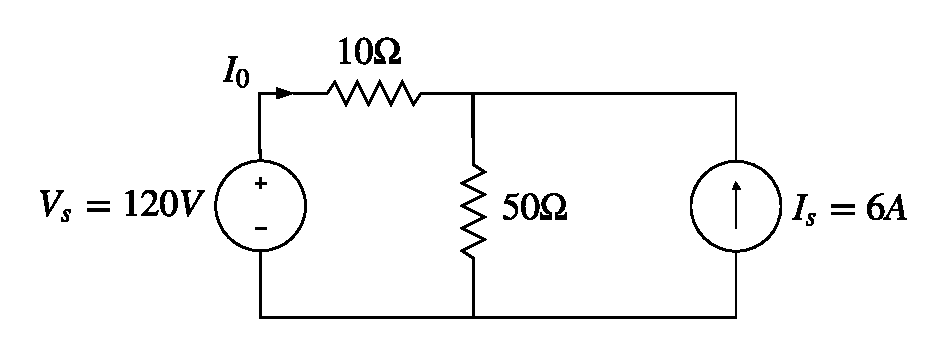
\includegraphics[width=0.8\textwidth]{exercices/ex-1-2}
\end{center}
\rep{$I_0=-3 A$}
\end{exwithsol}

\begin{exwithsol}{Association de r�sistances.}{solex:1-3}
\label{ex:1-3}
D�terminer la r�sistance �quivalente 
\begin{enumerate}
	\item � l'association en s�rie
	des $n$ r�sistances $R_1$, $R_2$, \ldots, $R_n$
	\item � l'association en parall�le
	des $n$ r�sistances $R_1$, $R_2$, \ldots, $R_n$
	\item du dip�le de la figure ci-dessous
	� l'aide de r�ductions successives d'associations d'�l�ments en s�rie
	ou en parall�le.
\end{enumerate}
\begin{center}
	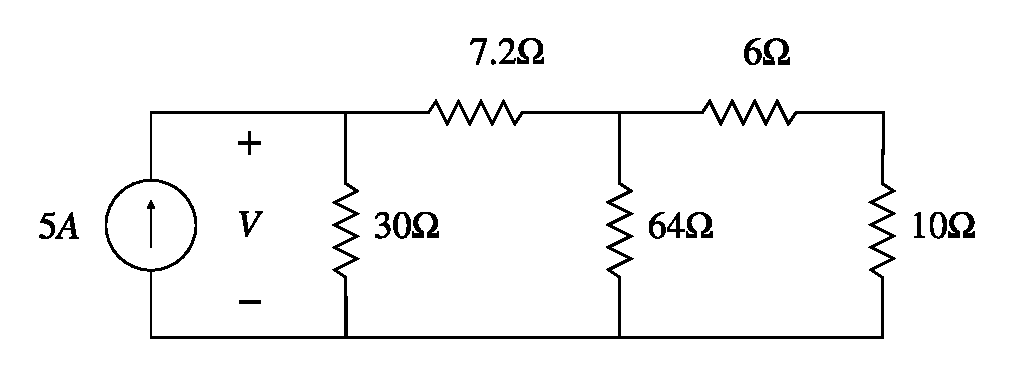
\includegraphics[width=0.8\textwidth]{exercices/ex-1-3}
\end{center}

\rep{1) $R_{eq}=R_1+R_2+\ldots +R_n$ \\
	2) $G_{eq}=G_1+G_2+\ldots +G_n$ \\
	3) $R_{eq} = 12\,\, \Omega$}
\end{exwithsol}

\begin{exwithsol}{Le diviseur potentiom�trique.}{solex:1-4}
\label{ex:1-4}
\begin{enumerate}
	\item D�terminer l'expression des tensions $V_1$ et $V_2$ aux bornes
	des r�sistances $R_1$ et $R_2$ du diviseur potentiom�trique de la
	figure ci-dessous.
	\item On alimente une r�sistance de charge $R_L$ par le tension
	$V_2$. D�terminer sous quelle condition la valeur de $V_2$ est peu
	influenc�e par la r�sistance de charge $R_L$.
\end{enumerate}
\begin{center}[h]
	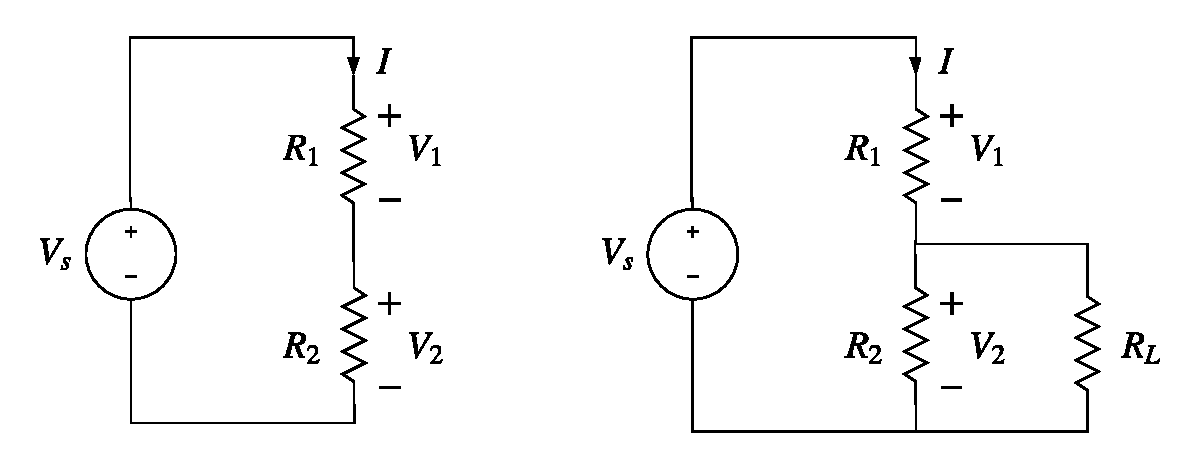
\includegraphics[width=\textwidth]{exercices/ex-1-4}
\end{center}
\end{exwithsol}


\begin{exwithsol}{Le diviseur de courant.}{solex:1-5}
\label{ex:1-5}
D�terminer l'expression des courants $I_1$ et $I_2$ parcourant les
r�sistances $R_1$ et $R_2$ de la figure ci-dessous.
\begin{center}
	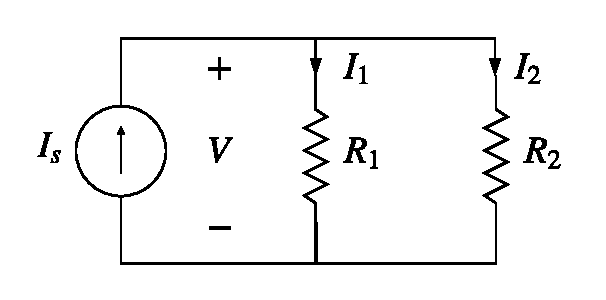
\includegraphics[width=0.55\textwidth]{exercices/ex-1-5}
\end{center}
\end{exwithsol}


\begin{exwithsol}{Sources r�elles de tension et de courant.}{solex:1-6}
\label{ex:1-6}
\begin{enumerate}
\item Montrer qu'une source r�elle de tension alimentant une r�sistance de
charge $R_L$ se comporte comme une source id�ale si $R_i \ll R_L$, cf. Figure~\ref{fig:source_de_tension_reelle}.
\item Montrer qu'une source r�elle de courant alimentant une r�sistance de
charge $R_L$ se comporte comme une source id�ale si $G_i \ll G_L$, cf. Figure~\ref{fig:source_courant}.
\end{enumerate}


\rep{Voir Section~\ref{sec:sie}}
\end{exwithsol}

\begin{exwithsol}{�quivalence de sources.}{solex:1-7}
\label{ex:1-7}
\begin{enumerate}
\item Montrer, comme indiqu� � la figure suivante, qu'un dip�le "source de tension" peut �tre
remplac� par un dip�le �quivalent "source de courant" si $I_s = \frac{V_s}{R_s}$ et $G_s = \frac{1}{R_s}$.
\begin{center}
	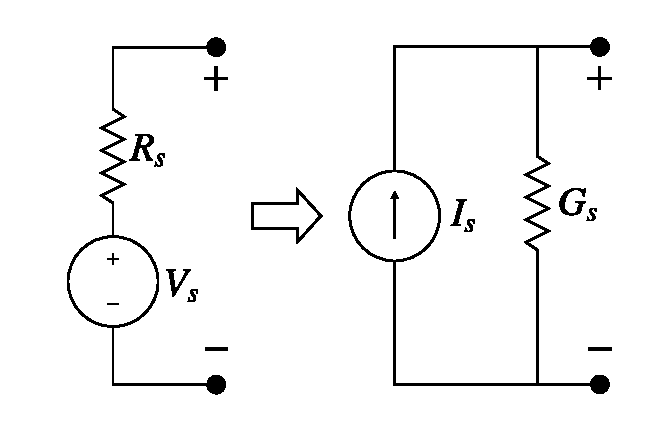
\includegraphics[width=0.5\linewidth]{exercices/ex-1-7-1}
\end{center}
\item Montrer, comme indiqu� � la figure suivante,  qu'inversement, un
dip�le "source de courant" peut �tre remplac� par un dip�le
�quivalent "source de tension" si $V_s = \frac{I_s}{G_s}$ et $R_s = \frac{1}{G_s}$.
\begin{center}
	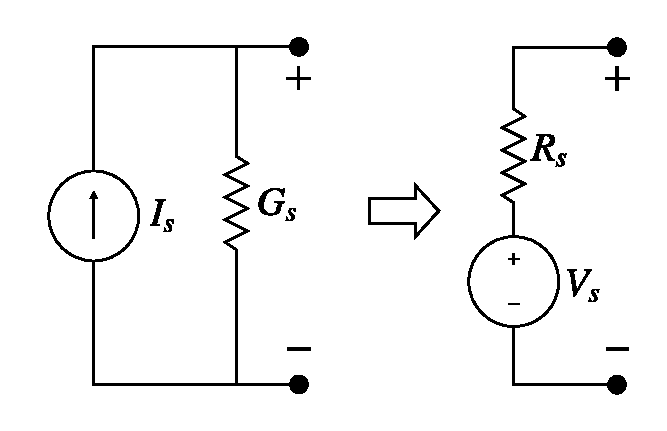
\includegraphics[width=0.5\linewidth]{exercices/ex-1-7-2}
\end{center}
\item Appliquer ces transformations pour r�duire le dip�le ci-dessous � un
dip�le �quivalent "source de tension" ou "source de courant".
\begin{center}
	\includegraphics[width=0.45\textwidth]{exercices/ex-1-7-3}
\end{center}
\end{enumerate}
\end{exwithsol}

\begin{exwithsol}{�quivalence de sources et r�duction.}{solex:1-8}
\label{ex:1-8}
\begin{enumerate}
	\item R�duire le circuit de la figure ci-dessous � un dip�le
	�quivalent comprenant une source de tension $V_{eq}$ en s�rie avec une r�sistance $R_{eq}$
	(dip�le ``source de tension �quivalente'').
	\item Si on connecte � l'acc�s  11$^{'}$ une r�sistance de charge  $R_L=10\,
	\Omega$, calculer la puissance absorb�e par $R_L$ ainsi que l'�tat
	�lectrique complet du circuit.
\end{enumerate}

\begin{center}
	\includegraphics[width=0.75\linewidth]{exercices/ex-1-8}
\end{center}


\rep{1) $V_{eq}= 13.125$ V, $R_{eq}=3.75\,\,\Omega$ \\
2) $p_{R_L}=9.112$ W}
\end{exwithsol}

\begin{exwithsol}{Source command�e.}{solex:1-9}
\label{ex:1-9}
Calculer la valeur de la source de tension $V_s$ de la figure ci-dessous si le courant
$I_{\phi}$ est �gal � 5 A.
\begin{center}
	\includegraphics[width=0.6\linewidth]{exercices/ex-1-9}
\end{center}

\rep{$V_s=50$ V}
\end{exwithsol}

\section{Solution des exercices}

\begin{solexercise}{\ref{ex:1-1}}
	\label{solex:1-1}
{\bf Circuit 1.} Choisissons le sens des courants $I$, $I_E$ et de la tension $U$ comme indiqu� ci-dessous.
\begin{center}
	\includegraphics[width=0.5\linewidth]{sol_exercices/ex1-1-1}
\end{center}
Vu la pr�sence de la source de tension, on a directement $U$ = 2 V.
La loi d'Ohm aux bornes d'une r�sistance s'�crit :\\[3mm]
\begin{minipage}[c]{0.5\textwidth}
	\begin{center}
		avec les sens conventionnels de r�f�rence\\[3mm]
		\begin{center}
			\includegraphics[width=0.4\linewidth]{sol_exercices/ex1-1-2}
		\end{center}
	\end{center}
	\[U=R.I\]
\end{minipage}
\begin{minipage}[c]{0.5\textwidth}
	\begin{center}
		avec les sens non conventionnels de r�f�rence\\[3mm]
		\begin{center}
			\includegraphics[width=0.3\linewidth]{sol_exercices/ex1-1-3}
		\end{center}
	\end{center}
	\[U=-R.I \]
\end{minipage}\\[3mm]
L'application de cette loi � la r�sistance $R=3\, \, \Omega$ donne
directement :
\[I=\frac{U}{3}=\frac{2}{3}\text{~A}\]
La premi�re loi de Kirchhoff (PLK) au noeud a s'�crit :
\[I+I_E-1=0 \qquad \text{on d�duit} \qquad
I_E=1-I=\frac{1}{3}\text{~A}\]
L'�tat �lectrique complet du circuit est connu. On en d�duit les
puissances consomm�es ou fournies par les diff�rents �l�ments. 
\begin{enumerate}
	\item R�sistance $R=3\,\, \Omega$ : les sens adopt�s pour $U$ et $I$
	sont les sens conventionnels de r�f�rence
	\[p_{R}=UI=RI^2=\frac{4}{3}\text{~W}\]
	est la puissance consomm�e par cette r�sistance.
	\item Source $J=1$ A : 
	
	\begin{minipage}[c]{3cm}
		\begin{center}
			\includegraphics[width=0.6\linewidth]{sol_exercices/ex1-1-4}
		\end{center}
	\end{minipage}
	\begin{minipage}[c]{7cm}
		le courant et la  tension aux bornes de cet �l�ment sont orient�s
		selon les sens de r�f�rence non conventionnels,
	\end{minipage}
	\[p_{J}=U.1=2\text{~W}\]
	est la puissance fournie par la source $J$.
	\item Source $E=2$ V : 
	
	\begin{minipage}[c]{3cm}
		\begin{center}
			\includegraphics[width=0.6\linewidth]{sol_exercices/ex1-1-5}
		\end{center}
	\end{minipage}
	\begin{minipage}[c]{7cm}
		le courant et la tension aux bornes de cet �l�ment sont orient�s
		selon les sens de r�f�rence conventionnels,
	\end{minipage}
	\[p_{E}=U.I_E=\frac{2}{3}\text{~W}\]
	est la puissance consomm�e par la source. La valeur trouv�e est
	positive, cette source consomme effectivement de la puissance.
	
	Si l'on avait adopt� les sens non conventionnels de r�f�rence, on
	aurait :\\[3mm]
	\begin{minipage}[c]{3cm}
		\begin{center}
			\includegraphics[width=0.6\linewidth]{sol_exercices/ex1-1-6}
		\end{center}
	\end{minipage}
	\begin{minipage}[c]{7cm}
		$I^{'}_E=-I_E$ et 
		$p^{'}_{E}=U.I^{'}_E=-\frac{2}{3}\text{~W}$
		est la puissance fournie par la source. Elle est n�gative indiquant
		que $E$ consomme  de la puissance. Quels que soient les sens adopt�s
		pour $U$ et $I$, on constate que les r�sultats sont coh�rents.
	\end{minipage}
\end{enumerate}
Le bilan de puissance s'�tablit comme suit :
\[\Sigma \text{p consomm�es}=0 \qquad p_E+p_R-p_J=0\]
ou
\[\Sigma \text{p consomm�es}=\Sigma \text{p fournies} \qquad
p_E+p_R=p_J\]


\noindent{\bf  Circuit 2.}

\begin{minipage}[c]{5cm}
	\begin{center}
		\includegraphics[width=\linewidth]{sol_exercices/ex1-1-7}
	\end{center}
\end{minipage}
\begin{minipage}[c]{5.5cm}
	Choisissons le sens des courants $I$, $I_E$ et des  tensions $U$ et $U_J$
	comme indiqu� ci-contre.
	
	Vu la pr�sence de la source de courant, on a directement $I$ = -1 A.
	
	Par application de la loi d'Ohm : $U=3.I=-3$ V.
	
	La seconde loi de Kirchhoff (SLK) s'�crit : \\$U+U_J-2=0 \, \Rightarrow\,
	U_J=$ 5 V.
\end{minipage}
On calcule les puissances relatives aux diff�rents �l�ments :
\begin{enumerate}
	\item $p_R=RI^2= 3$ W est la puissance consomm�e par la r�sistance de
	$3\,\, \Omega$.
	\item $p_J=1.U_J=$ 5 W est la puissance fournie par la source $J$.
	\item $p_E=2.I=-2$ W est la puissance fournie par $E$. Puisque la
	valeur est n�gative, $E$ est en fait consommatrice de puissance.
\end{enumerate}
Le bilan de puissance s'�crit :
\[p_R=p_J+p_E\]


\noindent{\bf Circuit 3.}

\begin{center}
	\includegraphics[width=0.6\linewidth]{sol_exercices/ex1-1-8}
\end{center}
On trouve :
\begin{gather*}
U_1=2\,\, \text{V}\, \quad U_3=-3\,\,\text{V},\quad
U_J=5\,\,\text{V}\\
I_1=2\,\, \text{A}\, \quad I_3=-1\,\, \text{A}\, \quad
I_E=1\,\,\text{A}
\end{gather*}
Puissances consomm�es par les r�sistances :
\[p_{1\Omega}=R_1I_1^2=4\,\, \text{W},\quad p_{3\Omega}=R_3I_3^2=3\,\,
\text{W}\]
Puissances fournies par les sources :
\[p_E=U_1.I_E=2 \,\, \text{W},\quad p_J=U_J.1=5\,\, \text{W}\]
Bilan de puissance :
\[p_{1\Omega}+p_{3\Omega}=p_E+p_J\]
\end{solexercise}

\begin{solexercise}{\ref{ex:1-2}}
	\label{solex:1-2}
Adoptant les sens des courants et tensions de la
Fig.~\ref{ex1-1sol}, on trouve successivement:
\begin{enumerate}
	\item par application de la PLK  au noeud b ou c :
	\[ I_1-I_0-6=0\]
	\item par  application de la SLK � la maille abca :
	\[120 - V_0 - V_1 = 0\]
	\item ou en appliquant la loi d'Ohm : 
	\[120 - 10I_0 - 50I_1 =0 \]
\end{enumerate}
On trouve finalement : $I_0=-3$ A et $I_1 = 3$ A.

\begin{figure}[h]
	\centering
	\includegraphics[width=0.7\linewidth]{sol_exercices/ex1-2-1}
	\caption{Lois de Kirchhoff et loi d'Ohm.}\label{ex1-1sol}
\end{figure}

On v�rifie le bilan de puissance : 
\begin{enumerate}
	\item puissance consomm�e par la r�sistance de 10 $\Omega$ : $$p_{10
		\Omega}= 10 I_0^2= 90~\text{W}$$
	\item puissance consomm�e par la r�sistance de 50 $\Omega$ : $$p_{50
		\Omega}= 50 I_1^2= 450~\text{W}$$
	\item puissance produite par la source de tension de 120 V : $$p_{120
		V}= 120 I_0= - 360~\text{W}$$
	cette source absorbe de la puissance !
	\item puissance produite par la source de courant de 6 A : $$p_{6A}
	= 6 V_1= 6.50.I_1 = 900~\text{W}$$
\end{enumerate}
On v�rifie bien que la puissance totale produite par les
deux sources = puissance totale consomm�e par les r�sistances: $$p_{10\Omega}+p_{50\Omega}=p_{120V}+p_{6A}.$$
\end{solexercise}
\\
\\
\begin{solexercise}{\ref{ex:1-3}}
	\label{solex:1-3}
{\bf �quivalence entre deux dip�les :}
{\em deux dip�les sont �quivalents si pour  une m�me
	d.d.p. aux bornes $v$, ces dipoles sont parcourus par un m�me courant
	$i$ et inversement si, pour un m�me courant inject� $i$, il appara�t une
	m�me d.d.p. $v$ aux bornes des deux dip�les.}

On ne change rien � l'�tat �lectrique d'un circuit si l'on
remplace un des dip�les le constituant par un dip�le �quivalent.

Nous appliquons ici ce principe au cas particulier de dip�les r�sistifs.

\noindent {\bf 1. Association en s�rie}\\
Aliment�es par une source de tension $V_s$, les r�sistances $R_1$,
$R_2$, \ldots , $R_n$ connect�es en s�rie sont parcourues par le m�me
courant $I_s$.
%\newpage

Nous recherchons une r�sistance �quivalente $R_{eq}$ telle que 
\begin{center}
\includegraphics[width=0.9\linewidth]{sol_exercices/ex1-3-1}
\end{center}
La SLK et la loi d'Ohm appliqu�es dans la maille fournissent :
\[V_s=R_1I_s+R_2I_s+\ldots + R_nI_s\quad \text{et}\quad
I_s=\frac{V_s}{R_1+R_2+\ldots + R_n}=\frac{V_s}{R_{eq}}\]
Finalement, la r�sistance �quivalente est donn�e par la somme des $n$
r�sistances
\[R_{eq}=R_1+R_2+\ldots +R_n\]

\noindent {\bf 2. Association en parall�le}\\
Il existe une m�me d.d.p. aux bornes de tous les �l�ments.
\begin{center}
	\includegraphics[width=0.9\linewidth]{sol_exercices/ex1-3-2}
\end{center}
On �crit :
\[V_s=R_1\, I_1 = R_2\, I_2 = \ldots = R_n\, I_n \]
\[I_s=I_1+I_2+ \ldots + I_n= V_s(\frac{1}{R_1}+\frac{1}{R_2}+ \ldots +
\frac{1}{R_n})\]
On peut repr�senter ce dip�le par une r�sistance �quivalente qui v�rifie :
\[\frac{I_s}{V_s}=\frac{1}{R_{eq}}=\frac{1}{R_1}+\frac{1}{R_2}+\ldots
+  \frac{1}{R_n}\]
ou en termes de conductances :
\[G_{eq}=G_1+G_2+ \ldots + G_n\]

\newpage
\noindent {\bf 3.}
On calcule successivement :
\begin{center}
	\includegraphics[width=0.9\linewidth]{sol_exercices/ex1-3-3}
\end{center}

\end{solexercise}

\begin{solexercise}{\ref{ex:1-4}}
	\label{solex:1-4}
\noindent{\bf 1. Expression de $V_1$ et $V_2$.}
On d�rive successivement :
\begin{align*}
I&=\frac{V_s}{R_1+R_2}\\
V_1&=R_1\,I=V_s\frac{R_1}{R_1+R_2}\\
V_2&=R_2\,I=V_s\frac{R_2}{R_1+R_2} 
\end{align*}

Le choix de $R_1$ et$R_2$ permet de fixer la mani�re dont $V_s$ est
r�partie entre $V_1$ et $V_2$. Il existe une infinit� de couples de valeurs $(R_1,R_2)$
donnant lieu � la m�me r�partition. Le choix des valeurs de ces deux
r�sistances est aussi guid� par :
\begin{enumerate}
	\item la puissance qui peut �tre dissip�e par chaque �l�ment;
	\item la r�sistance de charge �ventuelle que doit alimenter $V_1$ ou
	$V_2$ comme montr� au point~2.
\end{enumerate}
\noindent{\bf 2. Influence de $R_L$.}
On d�rive successivement :
\begin{align*}
V_2&=\frac{R_{eq}}{R_{eq}+R_1}V_s \quad \text{avec} \quad 
R_{eq}=\frac{R_2 R_L}{R_2 + R_L}\\
V_2 &= \frac{R_2}{R1[1+ (R_2/R_L)]+R_2}V_s
\end{align*}
Nous aurons donc 
\[\frac{V_2}{V_s}\simeq \frac{R_2}{R_1+R_2} \quad \text{si} \quad R_L \gg R_2.\]
\end{solexercise}

\begin{solexercise}{\ref{ex:1-5}}
	\label{solex:1-5}
La tension aux bornes des deux r�sistances est donn�e par 
\[V=I_s\frac{R_1 R_2}{R_1+R_2}\]
Le courant $I_s$ se divise donc comme suit :
\begin{align*}
I_1 &=\frac{V}{R_1}=I_s\frac{R_2}{R_1+R_2} \quad \text{ou} \quad
I_s\frac{G_1}{G_1+G_2}\\
I_2 &=\frac{V}{R_2}=I_s\frac{R_1}{R_1+R_2} \quad \text{ou} \quad
I_s\frac{G_2}{G_1+G_2}
\end{align*}
\end{solexercise}

\begin{solexercise}{\ref{ex:1-6}}
	\label{solex:1-6}
Voir Exercice pr�c�dent et /ou la Section~\ref{sec:sie}.
\end{solexercise}

\begin{solexercise}{\ref{ex:1-7}}
	\label{solex:1-7}
\noindent{\bf 1. �quivalence source de tension $\rightarrow$ source de
	courant.}
Les deux d�p�les sont �quivalents si ils d�livrent un m�me courant $I$
sous une m�me tension $V$.
Le courant d�bit� par le dip�le ``source de tension'' s'�crit :
	\[I= \frac{V_s}{R_s}-\frac{V}{R_s}\]
Le courant d�bit� par le dip�le ``source de courant'' vaut :
	\[I=I_s-G_s V\]
La condition d'�quivalence est :
\[\frac{V_s}{R_s}-\frac{V}{R_s}=I_s-G_s V\]
Les param�tres du dip�le ``source de courant'' �quivalent sont :
\begin{align*}
I_s&=\frac{V_s}{R_s}\\
G_s&=\frac{1}{R_s}
\end{align*}

\noindent{\bf 2. �quivalence source de courant $\rightarrow$ source de
	tension.}
Les deux dip�les sont �quivalents si ils pr�sentent une m�me tension $V$
sous un m�me courant $I$.
La condition d'�quivalence s'�crit donc :
\[\frac{I_s}{G_s}-\frac{I}{G_s}=V_s-R_s I\]
Les param�tres du dip�le ``source de tension'' �quivalent sont :
\begin{align*}
V_s&=\frac{I_s}{G_s}\\
R_s&=\frac{1}{G_s}
\end{align*}


\noindent{\bf 3. Exemple}
On transforme successivement le circuit comme suit.
\begin{center}
	\includegraphics[width=\linewidth]{sol_exercices/ex1-7}
\end{center}
\end{solexercise}

\begin{solexercise}{\ref{ex:1-8}}
	\label{solex:1-8}
\noindent{\bf 1. Source de tension �quivalente.}

On transforme successivement :
\begin{enumerate}
	\item la branche CB\\
	\includegraphics[width=0.4\linewidth]{sol_exercices/ex1-8-1}
	\item la branche DE\\
	\includegraphics[width=\linewidth]{sol_exercices/ex1-8-2}
\end{enumerate}
La partie du circuit situ�e au-dessus de AE se r�duit ainsi en la
forme
\begin{center}
	\includegraphics[width=\linewidth]{sol_exercices/ex1-8-4}
\end{center}
Connectant au reste du circuit, on a 
\begin{center}
	\includegraphics[width=\linewidth]{sol_exercices/ex1-8-3}
\end{center}

\noindent Finalement
\[V_{eq}=13.125\,\, \text{V}, \quad R_{eq}=3.75\,\, \Omega\]

\noindent{\bf 2. Acc�s 11$^{'}$ ferm� sur $R_L=10\,\, \Omega$.}

Le circuit �tant remplac� par son dip�le �quivalent ``source de tension'',  on connecte
la r�sistance de charge � l'acc�s 11$^{'}$.\\
\begin{minipage}[c]{0.3\textwidth}
	\includegraphics[width=\linewidth]{sol_exercices/ex1-8-5}
\end{minipage}
\begin{minipage}[c]{0.7\textwidth}
	On d�duit le courant d�bit� dans la r�sistance de charge :
	\[I=\frac{V_{eq}}{R_{eq}+R_L}=0.9545\,\, \text{A}\]
	La tension aux bornes de cette charge vaut :
	\[U=RI=10I=9.545\,\, \text{V}\]
	La puissance consomm�e par la charge vaut :
	\[p_{R_L}=R_L I^2=9.112\,\, \text{W}\]
\end{minipage}\\
\\
\noindent{\bf 3. �tat �lectrique complet du circuit}

Dans ce qui suit, les puissances calcul�es relatives aux r�sistances
sont les puissances consomm�es par ces r�sistances. Les puissances calcul�es
relatives aux sources de tension et de courant sont les puissances
fournies par ces sources au reste du circuit.

\begin{enumerate}
	\item branche AE :
	
	\begin{minipage}[c]{5cm}
		\begin{center}
			\includegraphics[width=0.7\linewidth]{sol_exercices/ex1-8-6}
		\end{center}
	\end{minipage}
	\begin{minipage}[c]{5cm}
		\begin{align*}
		I^{'}&=\frac{U}{5}=1.909\,\, \text{A}\\
		I_A&=I+I^{'}-3=-0.1365\,\, \text{A}\\\
		p_{J=3}&=3U=28.635\, \, \text{W}\\
		p_{R=5}&=5I^{'2}=18.22 \,\, \text{W}
		\end{align*}
	\end{minipage}
	\item dip�le AB :
	
	\begin{minipage}[c]{5cm}
		\begin{center}
			\includegraphics[width=0.4\linewidth]{sol_exercices/ex1-8-7}
		\end{center}
	\end{minipage}
	\begin{minipage}[c]{5cm}
		\begin{align*}
		p_{E=10}=10I_A = -1.365\, \, \text{W}
		\end{align*}
		Cette source consomme de la puissance.
	\end{minipage}
	\item dip�le BC :
	
	\begin{minipage}[c]{5cm}
		\begin{center}
			\includegraphics[width=0.55\linewidth]{sol_exercices/ex1-8-8}
		\end{center}
	\end{minipage}
	\begin{minipage}[c]{5cm}
		\begin{align*}
		U_{CB}&=5(I_A-2)= -10.682\, \, \text{V}\\
		p_{R=5}&=\frac{U_{CB}^2}{5}=22.823\, \, \text{W}\\
		p_{J=2}&=-2U_{CB}=21.365\, \, \text{W}
		\end{align*}
	\end{minipage}
	\item dip�le CD :
	
	\begin{minipage}[c]{5cm}
		\begin{center}
			\includegraphics[width=0.55\linewidth]{sol_exercices/ex1-8-9}
		\end{center}
	\end{minipage}
	\begin{minipage}[c]{5cm}
		\begin{align*}
		p_{R=5}=5I_A^2=0.093\, \, \text{W}
		\end{align*}
	\end{minipage}
	
	
	\item dip�le DE :
	
	\begin{minipage}[c]{5cm}
		\begin{center}
			\includegraphics[width=\linewidth]{sol_exercices/ex1-8-10}
		\end{center}
	\end{minipage}
	\begin{minipage}[c]{5cm}
		\begin{align*}
		U_{DE}&=U-10+U_{CB}+U_{DC}= -11.82\, \, \text{V}\\
		p_{J=2}&=-2U_{DE}=23.635\, \, \text{W}\\
		p_{R_1=10}&=\frac{U_{DE}^2}{10}= 13.971\, \, \text{W}\\
		p_{R_2=10}&=\frac{(U_{DE}+5)^2}{10}= 4.648\, \, \text{W}\\
		I_5&=\frac{U_{DE}+5}{10}=-0.682\, \, \text{A}\\
		p_{E=5}&=5I_5= -3.409\, \, \text{W}
		\end{align*}
		Cette source consomme de la puissance.
	\end{minipage}
\end{enumerate}
\end{solexercise}

\begin{solexercise}{\ref{ex:1-9}}
	\label{solex:1-9}
\begin{center}
	\includegraphics[width=0.7\linewidth]{sol_exercices/ex1-9}
\end{center}
La PLK appliqu�e aux noeuds a et b fournit :
\begin{align*}
I_s&=I_{\phi}+5 = 10\\
I_s&=6I_{\phi} + I_1 \quad \rightarrow \quad I_1 = I_s-6I_{\phi}=-20
\end{align*}
La SLK appliqu�e � la maille abca s'�crit :
\[\begin{array}[t]{ll}
V_s+V_1+V_2=0 \quad \text{avec} \quad & V_2=10I_{\phi} = 50\\
& V_1 = 5I_1= -100 \end{array}\]
Finalement : $V_s=50$ V.
\end{solexercise}
% !TeX encoding = ISO-8859-1
% !TeX spellcheck = fr_FR
% !TeX root = syllabus_ELEC0053.tex

\chapter{R�gimes transitoires}

\textit{Ce chapitre s'int�resse � l'analyse de circuits comportant  des �l�ments lin�aires et invariants $R$, $L$, $C$ et des sources ind�pendantes d'�nergie.
Nous traitons quelques probl�mes simples, relatifs � des circuits
localis�s, lin�aires et invariants du premier et du deuxi�me ordre, soumis � une excitation.
Nous avons d�lib�r�ment opt� pour la r�solution directe des �quations int�gro-diff�rentielles\footnote{Une autre approche consiste � utiliser la transform�e de Laplace, qui offre certains avantages, dont notamment la d�termination des conditions initiales qui devient automatique.} r�gissant ces circuits, la d�termination des constantes d'int�gration s'obtenant � partir des conditions aux limites dict�es par la physique des ph�nom�nes. }

\textit{Les ph�nom�nes transitoires sont des variations de
courant et/ou de tension dues � des variations brusques des tensions ou des
courants des sources d'alimentation (r�ponse forc�e), ou dues au fait que l'�nergie emmagasin�e dans les inductances (sous forme magn�tostatique) et condensateurs (sous forme �lectrostatique) est subitement rel�ch�e et dissip�e dans un circuit r�sistif (r�ponse libre).}


\section{Propri�t�s des �l�ments L et C lin�aires et invariants}

\paragraph{M�moire. }$C$ et $L$ ont une m�moire.
	Soit un condensateur excit� par un courant $i(t)$. On a 
	\[u(t)=\frac{1}{C}\int_{-\infty}^ti(x)dx\]
	$u(t)$ d�pend non seulement de $i$ � l'instant $t$ mais aussi de
	$i(x)$ pour $x< t$, soit de toute ''l'histoire'' du syst�me.
	
	On a aussi :
	{\small \[u(t)=u(t_0)+\frac{1}{C}\int_{t_0}^t i(x)dx\]}
	$u(t_0)$ r�sume tout le pass� du syst�me de $[-\infty,t_0]$.
		De m�me, pour une inductance excit�e par une tension $u(t)$
	\[
	i(t)=\frac{1}{L}\int_{-\infty}^tu(x)dx, \qquad
	i(t)=i(t_0)+\frac{1}{L}\int_{t_0}^tu(x)dx.\]

\paragraph{Continuit� de la tension aux bornes d'un condensateur.}
	Si le courant $i(t)$ induit par un condensateur est born� 
	$\forall t$, alors la tension aux bornes de ce condensateur est une grandeur continue.
	Ceci d�coule de la relation 
	\[u=\frac{1}{C}\int_{-\infty}^ti(x)dx.\]
	$u$ ne peut varier de mani�re instantan�e aux bornes d'un
	condensateur.
	Sinon, cela donne lieu � un courant infini (cas de l'impulsion de Dirac !).
	Il faut donc �viter de mettre sous tension brusquement un condensateur, ou de le court-circuiter.

	On suppose ici des \textbf{�l�ments id�aux}, c'est-�-dire \textbf{sans pertes} (voir point suivant). En tenant compte des pertes, le courant lors d'une mise sous tension brusque est tr�s important, mais reste born� !
	
\paragraph{Continuit� du courant dans une bobine.}
	Si la tension $u(t)$ aux bornes d'une inductance est born�e $\forall t$, 
	alors le courant dans cette inductance est une grandeur continue.
	Ceci d�coule de la relation \[i=\frac{1}{L}\int_{-\infty}^tu(x)dx,\]
	$i$ ne peut varier de mani�re instantan�e aux bornes d'une inductance.
	Sinon, il appara�t en th�orie une tension infinie (cas de l'impulsion de Dirac !), et en pratique un arc de courant si on tente d'ouvrir le circuit.
	Il faut donc en g�n�ral prendre des mesures sp�ciales pour couper le courant dans un circuit inductif.

\paragraph{$C$ et $L$ sont des �l�ments non-dissipatifs.}
	La puissance consomm�e par un condensateur est $$ 
	p_C(t)=u(t)i(t)=Cu\frac{du}{dt}.$$
	L'�nergie fournie au condensateur dans l'intervalle $t_1$, $t_2$ est donc
	\[w_C(t_1,t_2)=\int_{t_1}^{t_2}p(x)dx=\frac{1}{2}C(u^2(t_2)-u^2(t_1))\]
	et est ind�pendante de la forme du signal $u(t)$ dans l'intervalle
	$[t_1,t_2]$ ; 
	$w_C(t_1,t_2)$ d�pend seulement de la valeur de $u$ aux instants $t_1$ et $t_2$.
	
	Si consid�re un signal $u$ p�riodique de p�riode $T$, alors
	\[w_C(t_1,t_1+T) = 0\]
	Ceci implique que l'�l�ment ne dissipe pas d'�nergie : 
	\begin{itemize}
		\item durant une partie de la p�riode, $p(t)>0$, le condensateur
		stocke l'�nergie qui lui est fournie,
		\item durant le reste de la p�riode, $p(t)<0$, le condensateur
		restitue l'�nergie qu'il a stock�e.
	\end{itemize}
	Pour une inductance, on observe les m�mes propri�t�s :
	\begin{align*}
	p_L(t)&=Li\frac{di}{dt}\\
	w_L(t_1,t_2)& =\frac{1}{2}L(i^2(t_2)-i^2(t_1))
	\end{align*}
	Et pour un signal p�riodique, on a donc �galement
	\[w_L(t_1,t_1+T) = 0.\]
	
	
\begin{testexample}[Bobine soumise � une excitation en courant.]
Une inductance de 100 mH est aliment�e par une source de courant d�livrant un signal de courant de la forme (cf. Figure~\ref{fig:ex_ind}) :
$$i(t)=
	\left\{\begin{array}{ll}0 & t<0\\
	10te^{-5t}& t>0
	\end{array}\right.$$
L'�volution de la tension est donn�e par
$$u(t)=
	\left\{\begin{array}{ll} 0 & t<0\\
	e^{-5t}(1-5t)& t>0
	\end{array}\right.$$
celle de la puissance par 
$$p(t)=
\left\{\begin{array}{ll}0 & t<0\\
10t(1-5t)e^{-10t}& t>0
\end{array}\right.$$
et celle de l'�nergie par 
$$w(t)=
\left\{\begin{array}{ll}0 & t<0\\
5t^2e^{-10t}& t>0
\end{array}\right.$$
Dans l'intervalle $[0,0.2]$ s, l'inductance stocke une certaine �nergie ;
dans l'intervalle $[0.2,\infty]$ s, cette �nergie est restitu�e
On a  :
\begin{itemize}
	\item $w(t) \geq 0 \quad \forall t$ : �l�ment passif
	\item $w(\infty)=0$ : finalement aucune �nergie n'est dissip�e.
\end{itemize}
\end{testexample}
\begin{figure*}[bt]
	\centering
	\subfloat[Courant (excitation)]{\includegraphics[width=0.3\textwidth]{figs/figs_reg_trans/bobine_transitoire_courant.pdf}} 
	\subfloat[Tension]{\includegraphics[width=0.3\textwidth]{figs/figs_reg_trans/bobine_transitoire_tension.pdf}} \\
	\subfloat[Puissance]{\includegraphics[width=0.3\textwidth]{figs/figs_reg_trans/bobine_transitoire_puissance.pdf}} 
	\subfloat[�nergie]{\includegraphics[width=0.3\textwidth]{figs/figs_reg_trans/bobine_transitoire_energie.pdf}}
	\caption{�volution des diff�rentes grandeurs � travers ou aux bornes de la bobine en fonction du temps\label{fig:ex_ind}.}
\end{figure*}
	
\paragraph{�nergie emmagasin�e.}
Soit un condensateur $C$ port� initialement (en $t=0$) au potentiel
$V$.
On le connecte � un circuit ext�rieur $\cal R$ et il re�oit durant l'intervalle
$[0 , t_2]$, une quantit� d'�nergie :
\[w_C(0,t_2)=\frac{1}{2}C(u^2(t_2)-V^2)\]
Si $u(t_2)<V$, $w_C(0,t_2)<0$, cela  signifie que l'�nergie emmagasin�e
initialement dans le condensateur est rendue au circuit ext�rieur $\cal
R$.
L'�nergie maximale qui peut �tre extraite du condensateur est 
\[max|w_C(0,t_2)|=\frac{1}{2}CV^2.\]

Il est donc essentiel de retenir les constatations de la Table~\ref{tab:energie_LC} 

\begin{table}[h]
	\caption{Energie emmagasin�e dans un condensateur ou dans une bobine.\label{tab:energie_LC}}
	\begin{boxedminipage}{\linewidth}
		L'�nergie emmagasin�e dans
		\begin{itemize}
			\item un condensateur initialement port� au potentiel $V$ est $\frac{1}{2}CV^2$.
			\item une inductance initialement parcourue par un courant $I$ est $\frac{1}{2}LI^2$.
		\end{itemize}
	\end{boxedminipage}
\end{table}


\section{Les circuits du premier ordre}
\subsection{Circuit RC}
\begin{marginfigure}
\centering
\begin{tikzpicture}[y=-1cm]
\sf
\draw[black] (5.41111,3.46222) -- (5.36,3.30444) -- (5.25778,3.62222) -- (5.15556,3.30444) -- (5.05556,3.62222) -- (4.95333,3.30444) -- (4.85111,3.62222) -- (4.74889,3.30444) -- (4.64889,3.62222) -- (4.59778,3.46222);
\draw[black] (3.07111,3.46222) -- (3.02,3.30444) -- (2.91778,3.62222) -- (2.81556,3.30444) -- (2.71556,3.62222) -- (2.61333,3.30444) -- (2.51111,3.62222) -- (2.40889,3.30444) -- (2.30889,3.62222) -- (2.25778,3.46222);
\filldraw[black] (4.18889,3.47778) circle (0.06667cm);
\filldraw[black] (3.76667,5.15556) circle (0.06667cm);
\filldraw[black] (3.31111,3.48) circle (0.06667cm);
\draw[black] (3.07778,3.46667) -- (3.36667,3.46667);
\draw[black] (3.77778,3.91111) -- (3.56667,3.41333);
\draw[black] (4.6,3.47778) -- (4.18889,3.47778);
\path (0.82222,4.55556) node[text=black,anchor=base east] {$V_s$};
\path (2.63333,3.18889) node[text=black,anchor=base] {$R_s$};
\path (4.95556,3.22222) node[text=black,anchor=base] {$R$};
\path (4.27778,4.53333) node[text=black,anchor=base west] {$C$};
\path (3.33333,3.95556) node[text=black,anchor=base] {+};
\path (3.32222,5.1) node[text=black,anchor=base] {-};
\path (3.38889,4.58889) node[text=black,anchor=base east] {$u$};
\path (3.32222,3.3) node[text=black,anchor=base] {1};
\path (4.18889,3.3) node[text=black,anchor=base] {2};
\draw (1.02222,4.37778) -- (1.97333,4.37778);
\draw (1.34,4.53778) -- (1.65556,4.53778);
\draw (3.45333,4.37333) -- (4.08889,4.37333);
\draw (3.45333,4.52889) -- (4.08889,4.52889);
\draw (3.77111,4.53111) -- (3.77111,5.16667);
\draw (2.25556,3.46667) -- (1.49778,3.46667) -- (1.49778,4.06) -- (1.49778,4.37778);
\draw (3.77111,3.89556) -- (3.77111,4.37333);
\draw (1.49778,4.52889) -- (1.49778,4.84444) -- (1.49778,5.16667) -- (6.02222,5.16667) -- (6.02222,3.42222) -- (5.41111,3.42222);
\path (1.02222,4.22) node[anchor=base west] {+};
\path (1.02222,4.83778) node[anchor=base west] {-};

\end{tikzpicture}%

%% Configure (x)emacs for this file ...
%% Local Variables:
%% mode: latex
%% End:
\caption{Circuit illustrant les r�ponses forc�es et libres d'un circuit RC}
\label{fig:rcserie}
\end{marginfigure}
Soit le circuit de la Figure~\ref{fig:rcserie}.
\begin{enumerate}
	\item Si l'interrupteur bascule en position 1 : {\em r�ponse forc�e}, le 
	condensateur se charge. Port� finalement  au potentiel $V_s$, il emmagasine une
	�nergie
	\[w_C=\frac{1}{2}CV_s^2\]
	\item Si maintenant l'interrupteur bascule en position 2 : {\em r�ponse libre}, le condensateur se d�charge, l'�nergie emmagasin�e dans $C$ est progressivement relach�e et dissip�e dans la r�sistance.
\end{enumerate}


\paragraph{Charge du condensateur : r�ponse forc�e.}
\begin{marginfigure}
	\centering
	\begin{tikzpicture}[y=-1cm]
\sf
\draw[black] (3.07111,3.46222) -- (3.02,3.30444) -- (2.91778,3.62222) -- (2.81556,3.30444) -- (2.71556,3.62222) -- (2.61333,3.30444) -- (2.51111,3.62222) -- (2.40889,3.30444) -- (2.30889,3.62222) -- (2.25778,3.46222);
\filldraw[black] (3.35556,3.47778) circle (0.06667cm);
\filldraw[black] (3.76667,5.15556) circle (0.06667cm);
\draw[black] (3.07778,3.46667) -- (3.36667,3.46667);
\draw[black] (3.77778,3.91111) -- (3.35556,3.48889);
\draw[arrows=-triangle 45,black] (2.25778,3.81111) -- (3.05778,3.81111);
\path (0.82222,4.55556) node[text=black,anchor=base east] {$V_s$};
\path (2.63333,3.18889) node[text=black,anchor=base] {$R_s$};
\path (4.27778,4.53333) node[text=black,anchor=base west] {$C$};
\path (3.33333,3.95556) node[text=black,anchor=base] {+};
\path (3.32222,5.1) node[text=black,anchor=base] {-};
\path (3.38889,4.58889) node[text=black,anchor=base east] {$u$};
\path (3.32222,3.3) node[text=black,anchor=base] {1};
\path (2.51333,4.17778) node[text=black,anchor=base] {$i$};
\draw (1.02222,4.37778) -- (1.97333,4.37778);
\draw (1.34,4.53778) -- (1.65556,4.53778);
\draw (3.45333,4.37333) -- (4.08889,4.37333);
\draw (3.45333,4.52889) -- (4.08889,4.52889);
\draw (3.77111,4.53111) -- (3.77111,5.16667);
\draw (2.25556,3.46667) -- (1.49778,3.46667) -- (1.49778,4.06) -- (1.49778,4.37778);
\draw (3.77111,3.89556) -- (3.77111,4.37333);
\draw (1.49778,4.52889) -- (1.49778,4.84444) -- (1.49778,5.16667) -- (3.81333,5.16667);
\path (1.02222,4.22) node[anchor=base west] {+};
\path (1.02222,4.83778) node[anchor=base west] {-};

\end{tikzpicture}%

%% Configure (x)emacs for this file ...
%% Local Variables:
%% mode: latex
%% End:
	\caption{Partie gauche de la figure \ref{fig:rcserie}}
\end{marginfigure}
On suppose le condensateur initialement relax� (il ne porte aucune �nergie).
En $t=0$, l'interrupteur bascule en position 1 (cf. Figure~\ref{fig:rcserie}).
Pour $t<0$, $u(t)=0$.
Ensuite, en appliquant la PLK au noeud $1$, on a 
$$C\frac{du}{dt}+\frac{u-V_s}{R_s}=0,$$
ou encore 
$$\frac{du}{dt}+\frac{u}{CR_s}=\frac{V_s}{CR_s}.$$
Il s'agit d'une �quation diff�rentielle du premier ordre � coefficients constants, qui accepte une solution du type
\[u(t)=Ke^{-t/\tau_s}+V_s.\]
Reste � d�terminer la constante $K$. Or, $u(0-)=0$, donc $u(0+)=0$ par continuit� de $u$ et finalement 
$$ K=-V_s$$
Il vient finalement (cf. Figure \ref{fig:RC_u})
\begin{center}
	\fbox{
		$u(t)=V_s(1- e^{-t/\tau_s}),\qquad 
		t > 0$}
\end{center}
\begin{figure}[tb]
	\centering
	\includegraphics[width=0.7\textwidth]{figs/figs_reg_trans/RC_rep_forcee.pdf}
	\caption{R�ponse forc�e d'un circuit RC: tension. \label{fig:RC_u}}
\end{figure}
On peut �galement r��crire l'�volution de $u(t)$ pour mettre en �vidence le \textit{r�gime permanent}, et le \textit{r�gime transitoire}: 
\begin{eqnarray*}
	u(t)& = & V_s - V_s e^{-t/\tau_s}\\
	& = & \text{r�gime permanent (DC)~} + \text{~r�gime transitoire}.
\end{eqnarray*}

La \textit{constante de temps} $\tau_s=R_s C$ caract�rise la vitesse de la
charge. Au-del� de $5\tau_s$, le r�gime transitoire est n�gligeable et
$u(t)\simeq V_s$.
Quant au courant de charge, on le d�duit simplement (cf. Figure~\ref{fig:RC_i})
\[i(t)=C\frac{du}{dt}=\frac{V_s}{R_s}e^{-t/\tau_s}\]
\[i(0-)=0,\quad i(0+)=\frac{V_s}{R_s}=i_0.\]
\begin{figure}[ht]
	\centering
	\includegraphics[width=0.6\textwidth]{figs/figs_reg_trans/RC_courant_charge.pdf}
	\caption{R�ponse forc�e d'un circuit RC: courant.\label{fig:RC_i}}
\end{figure}

\paragraph{Bilan �nerg�tique.}
On peut s'int�resser au bilan �nerg�tique de l'op�ration de charge avec ce circuit:
\begin{enumerate}
	\item 	�nergie dissip�e dans la r�sistance $R_s$ :
	\[p_R(t)=\frac{V_s^2}{R_s}e^{-2t/R_sC}, \quad w_R(\infty)=\int_0^\infty
	p_R(t)dt= \frac{V_s^2C}{2}\]
	Cette quantit� est ind�pendante de $R_s$ !
	\item �nergie emmagasin�e dans le condensateur :
	\[p_C(t)=\frac{V_s^2}{R_s}e^{-t/R_sC}(1-e^{-t/R_sC}), \quad 
	w_C(\infty)=\int_0^\infty
	p_C(t)dt= \frac{V_s^2C}{2} = w_R \text{~!!}\]
	\item �nergie fournie par la source :\\
	\[w_V=w_R+w_C=V_s\int_0^\infty i(t)dt=V_s^2C\]
	\item Le \textit{rendement} de l'op�ration de charge est  $\eta=\frac{w_C}{w_V}=0.5$, ind�pendant de $R_s$ et de $C$ !
\end{enumerate}

\paragraph{D�charge du condensateur, r�ponse libre.}
\begin{marginfigure}
	\centering
	\begin{tikzpicture}[y=-1cm]
\sf
\draw[black] (5.41111,3.46222) -- (5.36,3.30444) -- (5.25778,3.62222) -- (5.15556,3.30444) -- (5.05556,3.62222) -- (4.95333,3.30444) -- (4.85111,3.62222) -- (4.74889,3.30444) -- (4.64889,3.62222) -- (4.59778,3.46222);
\filldraw[black] (4.18889,3.47778) circle (0.06667cm);
\filldraw[black] (3.76667,5.15556) circle (0.06667cm);
\draw[black] (4.6,3.47778) -- (4.18889,3.47778);
\draw[black] (4.18667,3.47778) -- (3.76444,3.9);
\draw[arrows=-triangle 45,black] (4.53333,3.81111) -- (5.68889,3.81111);
\path (4.95556,3.22222) node[text=black,anchor=base] {$R$};
\path (4.27778,4.53333) node[text=black,anchor=base west] {$C$};
\path (3.33333,3.95556) node[text=black,anchor=base] {+};
\path (3.32222,5.1) node[text=black,anchor=base] {-};
\path (3.38889,4.58889) node[text=black,anchor=base east] {$u$};
\path (4.15556,3.34444) node[text=black,anchor=base] {2};
\path (5.21111,4.17778) node[text=black,anchor=base] {$i$};
\draw (3.45333,4.37333) -- (4.08889,4.37333);
\draw (3.45333,4.52889) -- (4.08889,4.52889);
\draw (3.77111,4.53111) -- (3.77111,5.16667);
\draw (3.77111,3.89556) -- (3.77111,4.37333);
\draw (3.77778,5.16667) -- (6.02222,5.16667) -- (6.02222,3.42222) -- (5.41111,3.42222);

\end{tikzpicture}%

%% Configure (x)emacs for this file ...
%% Local Variables:
%% mode: latex
%% End:
	\caption{Partie droite de la figure \ref{fig:rcserie}.}
\end{marginfigure}
Apr�s un temps suffisamment long (suppos� infini, donc $u(t)= V_s$),
l'interrupteur bascule en position $2$. Soit $t=0$ cet instant. On a alors
\[C\frac{du}{dt}+\frac{u}{R}=0,\]
ou encore 
\[\frac{du}{u}=-\frac{dt}{RC}\]
et donc
\[u(t)=Ke^{-t/RC}=Ke^{-t/\tau}.\]
On d�termine la constante $K$ en utilisant le fait que $u(0-)=V_s$, donc $u(0+)=V_s$ par continuit� de $u$, et $K=V_s$.
On a donc finalement
\begin{center}
	\fbox{
		$u(t)=V_s e^{-t/RC}\,, \quad i(t)=\frac{V_s}{R}e^{-t/RC} \, , \qquad  t> 0$}
\end{center}
\begin{marginfigure}
\centering
\includegraphics[width=0.98\textwidth]{figs/figs_reg_trans/RC_tension_decharge.pdf}
\caption{R�ponse libre d'un circuit RC: tension.}
\end{marginfigure}
On peut � nouveau d�finir la constante de temps comme
\begin{center}
	\fbox{$\tau=RC$}
\end{center}
\begin{itemize}
	\item apr�s $\tau$ s, la tension est r�duite d'un facteur $e$ ($\simeq 0.368 V_s$)
	\item apr�s $5\tau$ s, la tension est r�duite � moins de $1$\% de sa valeur initiale
	\item $\frac{V_s}{\tau}$ = la pente de la tangente en $t=0$ de la courbe $u(t)$ 
	\item $-\frac{1}{\tau}$, la racine du polyn�me caract�ristique, est  appel�e la {\em fr�quence naturelle}   du circuit.
\end{itemize}
La puissance absorb�e par la r�sistance est
\[p(t)=Ri^2(t)=\frac{V_s^2}{R}e^{-2t/\tau} \, > \, 0 \quad \forall t\]
L'�nergie dissip�e dans l'intervalle $[0,t]$ est
\[w(t)=\int_0^t p(x)dx=\int_0^t\frac{V_s^2}{R}e^{-2x/\tau}dx=\frac{1}{2}CV_s^2(1-e^{-2t/\tau}),\]
et 
\[\lim_{t\rightarrow \infty}w(t)=\frac{1}{2}CV_s^2.\]
L'�nergie initialement emmagasin�e dans le condensateur est
finalement enti�rement dissip�e dans la r�sistance  � une vitesse
fix�e par la constante de temps $\tau$.


Int�ressons-nous maintenant au cas o� le condensateur est mis sous tension brusque alors qu'il est initialement charg�.
En $t=0$, le condensateur porte une charge initiale
$q_0$, c'est-�-dire pr�sente une d.d.p. $u_0=q_0/C$, et 
\begin{marginfigure}
\centering
\begin{tikzpicture}[y=-1cm]
\sf
\draw[black] (3.07111,3.46222) -- (3.02,3.30444) -- (2.91778,3.62222) -- (2.81556,3.30444) -- (2.71556,3.62222) -- (2.61333,3.30444) -- (2.51111,3.62222) -- (2.40889,3.30444) -- (2.30889,3.62222) -- (2.25778,3.46222);
\filldraw[black] (3.35556,3.47778) circle (0.06667cm);
\filldraw[black] (3.76667,5.15556) circle (0.06667cm);
\draw[black] (3.07778,3.46667) -- (3.36667,3.46667);
\draw[black] (3.77778,3.91111) -- (3.35556,3.48889);
\draw[arrows=-triangle 45,black] (2.25778,3.81111) -- (3.05778,3.81111);
\path (0.82222,4.55556) node[text=black,anchor=base east] {$V_s$};
\path (2.63333,3.18889) node[text=black,anchor=base] {$R_s$};
\path (4.27778,4.53333) node[text=black,anchor=base west] {$C$};
\path (3.33333,3.95556) node[text=black,anchor=base] {+};
\path (3.32222,5.1) node[text=black,anchor=base] {-};
\path (3.38889,4.58889) node[text=black,anchor=base east] {$u$};
\path (3.32222,3.3) node[text=black,anchor=base] {1};
\path (2.51333,4.17778) node[text=black,anchor=base] {$i$};
\draw (1.02222,4.37778) -- (1.97333,4.37778);
\draw (1.34,4.53778) -- (1.65556,4.53778);
\draw (3.45333,4.37333) -- (4.08889,4.37333);
\draw (3.45333,4.52889) -- (4.08889,4.52889);
\draw (3.77111,4.53111) -- (3.77111,5.16667);
\draw (2.25556,3.46667) -- (1.49778,3.46667) -- (1.49778,4.06) -- (1.49778,4.37778);
\draw (3.77111,3.89556) -- (3.77111,4.37333);
\draw (1.49778,4.52889) -- (1.49778,4.84444) -- (1.49778,5.16667) -- (3.81333,5.16667);
\path (1.02222,4.22) node[anchor=base west] {+};
\path (1.02222,4.83778) node[anchor=base west] {-};

\end{tikzpicture}%

%% Configure (x)emacs for this file ...
%% Local Variables:
%% mode: latex
%% End:
\caption{Partie gauche de la figure \ref{fig:rcserie}.}
\end{marginfigure}
\begin{eqnarray*}
	V_s & =& R_si+\frac{1}{C}\int_{-\infty}^t i\,  dt\\
	& = & R_s i+u_0+\frac{1}{C}\int_{0}^t i\,  dt
\end{eqnarray*}
\begin{marginfigure}
\centering
\begin{tikzpicture}[y=-1cm]
\sf
\path (4.27778,4.53333) node[text=black,anchor=base west] {$C$};
\path (3.06667,5.37778) node[text=black,anchor=base east] {$u_0$};
\draw (3.29556,5.16222) -- (4.24667,5.16222);
\draw (3.61333,5.32222) -- (3.92889,5.32222);
\path (3.29556,5.00444) node[anchor=base west] {+};
\path (3.29556,5.62222) node[anchor=base west] {-};
\draw (3.45333,4.37333) -- (4.08889,4.37333);
\draw (3.45333,4.52889) -- (4.08889,4.52889);
\draw (3.77111,4.53111) -- (3.77111,5.16667);
\draw (3.77111,3.89556) -- (3.77111,4.37333);
\draw (3.77111,5.32889) -- (3.77111,5.80667);

\end{tikzpicture}%

%% Configure (x)emacs for this file ...
%% Local Variables:
%% mode: latex
%% End:
\caption{Mod�lisation d'un condensateur initialement charg�.}
\end{marginfigure}
Le condensateur initialement charg� peut �tre remplac� par un
condensateur initialement relax� en s�rie avec une source de tension
constante $u_0$.
On peut v�rifier que la tension aux bornes du condensateur est donn�e par :
\begin{align*}
	u(t) & = V_s(1- e^{-t/\tau_s}) + u_0 e^{-t/\tau_s} \\ 
	&= \text{r�ponse forc�e~}+ \text{~r�ponse libre}.
\end{align*}


\subsection{Circuit RL}

\begin{marginfigure}
\centering
\begin{tikzpicture}[y=-1cm]
\sf
\draw[black] (5.41111,3.17778) -- (5.36,3.02) -- (5.25778,3.33778) -- (5.15556,3.02) -- (5.05556,3.33778) -- (4.95333,3.02) -- (4.85111,3.33778) -- (4.74889,3.02) -- (4.64889,3.33778) -- (4.59778,3.17778);
\draw[black] (3.07111,3.18) -- (3.02,3.02222) -- (2.91778,3.34) -- (2.81556,3.02222) -- (2.71556,3.34) -- (2.61333,3.02222) -- (2.51111,3.34) -- (2.40889,3.02222) -- (2.30889,3.34) -- (2.25778,3.18);
\filldraw[black] (3.76667,5.15556) circle (0.06667cm);
\filldraw[black] (3.35556,3.15556) circle (0.06667cm);
\filldraw[black] (4.18889,3.16667) circle (0.06667cm);
\draw[black] (3.07778,3.17778) -- (3.36667,3.17778);
\draw[black] (3.79556,3.62667) -- (3.6,3.10222);
\draw[black] (4.6,3.15556) -- (4.18889,3.15556);
\path (0.82222,4.55556) node[text=black,anchor=base east] {$V_s$};
\path (3.33333,3.95556) node[text=black,anchor=base] {+};
\path (3.32222,5.1) node[text=black,anchor=base] {-};
\path (3.36667,2.96667) node[text=black,anchor=base] {1};
\path (4.18889,2.95556) node[text=black,anchor=base] {2};
\path (4.95556,2.82222) node[text=black,anchor=base] {$R$};
\path (2.57778,2.82222) node[text=black,anchor=base] {$R_s$};
\path (3.38,4.57778) node[text=black,anchor=base] {$u$};
\draw (3.78667,4.01556) +(-97:0.16566) arc (-97:134:0.16566);
\draw (3.78,4.27333) +(-127:0.17601) arc (-127:128:0.17601);
\draw (3.78,4.55111) +(-127:0.17601) arc (-127:128:0.17601);
\draw (3.78667,4.80667) +(97:0.16345) arc (97:-134:0.16345);
\draw (1.02222,4.37778) -- (1.97333,4.37778);
\draw (1.34,4.53778) -- (1.65556,4.53778);
\draw (3.76667,3.6) -- (3.76667,3.85111);
\draw (3.76667,4.96889) -- cycle;
\draw (3.76667,4.96889) -- (3.76667,5.15556);
\draw (1.49778,4.52889) -- (1.49778,4.84444) -- (1.49778,5.16667) -- (6.02222,5.16667) -- (6.02222,3.13333) -- (5.41333,3.13333);
\draw (2.25556,3.18444) -- (1.49778,3.18444) -- (1.49778,3.77778) -- (1.49778,4.37778);
\path (1.02222,4.22) node[anchor=base west] {+};
\path (1.02222,4.83778) node[anchor=base west] {-};

\end{tikzpicture}%

%% Configure (x)emacs for this file ...
%% Local Variables:
%% mode: latex
%% End:
\caption{Circuit illustrant les r�ponses forc�es et libres d'un circuit RL.}
\label{figRLserie}
\end{marginfigure}
Soit le circuit de la Figure~\ref{figRLserie}.
\begin{enumerate}
	\item Si l'interrupteur bascule en position 1 : {\em r�ponse forc�e}, un
	courant dans l'inductance s'�tablit : $i_{\infty}=\frac{V_s}{R_s}$. L'�nergie
	magn�tique emmagasin�e vaut :
	\[w_L=\frac{1}{2}Li_{\infty}^2\]
	\item Si maintenant l'interrupteur bascule en position 2 : {\em r�ponse libre}, l'�nergie
	emmagasin�e dans $L$ est progressivement rel�ch�e et dissip�e dans la
	r�sistance.
\end{enumerate}


\paragraph{�tablissement du courant : r�ponse forc�e.}
On suppose l'inductance initialement relax�e. En $t=0$,
l'interrupteur bascule en position 1. Le syst�me r�pond donc � un �chelon de tension.
\begin{marginfigure}
\centering
\begin{circuitikz}[american voltages, scale = 1]
\draw
(0,0)
to[battery1, v=$V_s$] ++(0,1.8)
to[R, l=$R_s$, -o] ++(2,0) node[above]{1}
to [open] ++(0.5, 0) coordinate (A)
to [open] ++(0.5, 0) node[above]{2}  
to [R, l=$R$, o-]  ++(2,0) 
to [short] ++(0,-1.8)
--(0,0)
(A)
to [open] ++ (0,-0.5) coordinate (B)
to[L, l^=$L$, v_=$u$, -*] ++(0,-1.3)
(B) to [short, i<_=\textcolor{myRed}{$i$}, -*] ++ (-0.5, 0.5)
;
\end{circuitikz}

\caption{R�ponse forc�e d'un circuit RL.}
\end{marginfigure}
Pour $t<0$, $i(t)=0$. Ensuite par la SLK dans la maille d'int�r�t, 
\[L\frac{di}{dt}+R_s\, i=V_s,\]
ou encore 
\[i(t)=Ke^{-t/\tau_s}+\frac{V_s}{R_s}.\]
Pour d�terminer la constante $K$, on sait que 
$i(0-)=0$, donc $i(0+)=0$ par continuit� de $i$, et 
\begin{center}
	\fbox{
		$i(t)=\frac{V_s}{R_s}(1- e^{-t/\tau_s})=i_{\infty}(1-
		e^{-t/\tau_s})\quad t>0$}
	
	$\lim_{t\rightarrow \infty}i(t)=\frac{V_s}{R_s}=i_{\infty}$
\end{center}
\begin{figure}[h]
	\centering
	\includegraphics[width=0.6\textwidth]{figs/figs_reg_trans/RL_courant_reponse_forcee.pdf}
	\caption{R�ponse forc�e d'un circuit RL, courant.}
\end{figure}
L'inductance ``freine'' l'�tablissement  du courant.
La rapidit� de cet �tablissement  est dict�e par la constante
de temps $\tau_s=\frac{L}{R_s}$.
\begin{eqnarray*}
	i(t)& =& i_{\infty}(1- e^{-t/\tau_s})\\
	& = & i_{\infty} - i_{\infty} e^{-t/\tau_s}\\
	& = & \text{r�gime permanent (DC)~} + \text{~r�gime transitoire}
\end{eqnarray*}
La tension aux bornes de l'inductance est 
\[u(t)=L\frac{di}{dt}=V_s e^{-t/\tau_s}, \]
avec
\[u(0-)=0\quad u(0+)=V_s.\]
\begin{figure}[h]
	\centering
	\includegraphics[width=0.6\textwidth]{figs/figs_reg_trans/RL_tension_reponse_forcee.pdf}
	\caption{R�ponse forc�e d'un circuit RL, tension.}
\end{figure}

\paragraph{R�ponse libre.}
\begin{marginfigure}
	\centering
	\begin{circuitikz}[american voltages, scale = 1]
	\draw
	(0,0)
	to[battery1, v=$V_s$] ++(0,1.8)
	to[R, l=$R_s$, -o] ++(2,0) node[above]{1}
	to [open] ++(0.5, 0) coordinate (A)
	to [open] ++(0.5, 0) node[above]{2}  
	to [R, l=$R$, o-]  ++(2,0) 
	to [short] ++(0,-1.8)
	--(0,0)
	(A)
	to [open] ++ (0,-0.5) coordinate (B)
	to[L, l^=$L$, v_=$u$, -*] ++(0,-1.3)
	(B) to [short, i_=\textcolor{myRed}{$i$}, -*] ++ (+0.5, 0.5)
	;
\end{circuitikz}

	\caption{R�ponse libre d'un circuit RL.}
\end{marginfigure}
Apr�s un temps suffisamment long (suppos� infini, $i(t)= \frac{V_s}{R_s}=i_{\infty}$),
l'interrupteur bascule en position 2. Soit $t=0$ cet instant.
On a 
\[L\frac{di}{dt}+R\, i=0\]
\[\frac{di}{i}=-\frac{R\,dt}{L}\]
\[i(t)=Ke^{-(R/L)t}=Ke^{-t/\tau}\]
D�termination de la constante K :
\begin{itemize}
	\item $i(0-)=i_{\infty}\quad \rightarrow \quad i(0+)=i_{\infty}$ (continuit� de $i$)
	\item $u(0-)=0,\quad u(0+)=R\, i_{\infty}$
\end{itemize}
\begin{center}
	\fbox{
		$i(t)=i_{\infty}e^{-(R/L)t},\qquad u(t)=- R\, i_{\infty} e^{-(R/L)t} \quad t>0$}
\end{center}

\begin{marginfigure}
\centering
\includegraphics[width=0.98\textwidth]{figs/figs_reg_trans/RL_courant_reponse_libre.pdf}
\caption{R�ponse libre d'un circuit RL: courant.}
\end{marginfigure}
La constante de temps est 
$$\boxed{\tau=\frac{L}{R}}$$
\[i(t)=i_{\infty} e^{-t/\tau}\]
\[u(t)=i_{\infty}\, Re^{-t/\tau}\]
La fr�quence naturelle du circuit est  $-\frac{1}{\tau}=-\frac{R}{L}$


En ce qui concerne l'�nergie dissip�e dans la r�sistance, la puissance absorb�e par la r�sistance vaut
\[p(t)=Ri^2(t)=R\, i_{\infty}^2 e^{-2t/\tau} \, > \, 0 \quad \forall t.\]
Donc l'�nergie dissip�e dans l'intervalle $[0,t]$ est 
\[w(t)=\int_0^t p(x)dx=\frac{1}{2}L\,i_{\infty}^2(1-e^{-2t/\tau})\]
\[\lim_{t\rightarrow \infty}w(t)=\frac{1}{2}L\, i_{\infty}^2\]
L'�nergie initialement emmagasin�e dans l'inductance est
finalement enti�rement dissip�e dans la r�sistance � une vitesse
fix�e par la constante de temps $\tau$.

\begin{marginfigure}
	\centering
	\begin{tikzpicture}[y=-1cm]
\sf
\draw[black] (2.48889,2.53333) -- (2.48889,1.97778);
\draw[black] (2.47778,4.03333) -- (2.47778,4.46667);
\draw[arrows=triangle 45-,black] (2.01111,3.47778) -- (2.01111,3.02222);
\path (3.25556,3.42222) node[text=black,anchor=base west] {$L$};
\path (1.52222,3.35556) node[text=black,anchor=base east] {$i_0$};
\draw[black] (2.01333,3.24667) circle (0.33111cm);
\draw (2.95111,2.88222) +(-97:0.16566) arc (-97:134:0.16566);
\draw (2.94444,3.14) +(-127:0.17601) arc (-127:128:0.17601);
\draw (2.94444,3.41778) +(-127:0.17601) arc (-127:128:0.17601);
\draw (2.95111,3.67333) +(97:0.16345) arc (97:-134:0.16345);
\draw (2.93111,3.83556) -- cycle;
\draw (1.97778,2.93333) -- (1.97778,2.53333) -- (2.93111,2.53333) -- (2.93111,2.71778);
\draw (2.93111,3.83556) -- (2.93111,4.02222) -- (1.98889,4.02222) -- (1.98889,3.56667);

\end{tikzpicture}%

%% Configure (x)emacs for this file ...
%% Local Variables:
%% mode: latex
%% End:
	\caption{Mod�lisation d'une inductance initialement parcourue par un courant.}
\end{marginfigure}
Si on s'int�resse � l'�tablissement du courant dans une inductance parcourue par un courant initial $i_0$, on a
\begin{eqnarray*}
	\frac{V_s}{R_s} & =& \frac{u}{R_s}+\frac{1}{L}\int_{-\infty}^t u\,  dt\\
	& = & \frac{u}{R_s}+i_0+\frac{1}{L}\int_{0}^t u\,  dt
\end{eqnarray*}
L'inductance initialement parcourue par un courant peut �tre remplac�e par une
inductance initialement relax�e en parall�le avec une source de courant
con\-stant $i_0$.
On peut v�rifier que le courant parcourant l'inductance est donn� par 
\begin{eqnarray*}
	i(t) & = & \frac{V_s}{R_s}(1- e^{-t/\tau_s}) + i_0 e^{-t/\tau_s}= 
	\text{r�ponse forc�e~}+ \text{~r�ponse libre}.
\end{eqnarray*}



\section{Les circuits du deuxi�me ordre}
\subsection{R�ponse libre}
\begin{marginfigure}
	\centering
	\begin{tikzpicture}[y=-1cm]
\sf
\draw[black] (3.07111,3.18) -- (3.02,3.02222) -- (2.91778,3.34) -- (2.81556,3.02222) -- (2.71556,3.34) -- (2.61333,3.02222) -- (2.51111,3.34) -- (2.40889,3.02222) -- (2.30889,3.34) -- (2.25778,3.18);
\draw[black] (6.01111,3.17778) -- (6.01111,4.16667);
\draw[black] (4.18889,3.17778) -- (3.05556,3.17778);
\draw[black] (5.28889,3.2) -- (6.03333,3.2);
\draw[black] (3.07778,3.17778) -- cycle;
\draw[arrows=triangle 45-,black] (1.96667,3.52222) -- (3.25556,3.52222);
\path (2.57778,2.82222) node[text=black,anchor=base] {$R$};
\path (6.48889,4.4) node[text=black,anchor=base west] {$C$};
\path (2.48889,3.93333) node[text=black,anchor=base] {$i$};
\path (5.51111,3.64444) node[text=black,anchor=base] {+};
\path (5.51111,4.95556) node[text=black,anchor=base] {-};
\path (5.56667,4.36667) node[text=black,anchor=base east] {$u_{C0}$};
\path (4.74444,2.84444) node[text=black,anchor=base] {$L$};
\path (4.04444,2.95556) node[text=black,anchor=base east] {-};
\path (5.37778,2.97778) node[text=black,anchor=base east] {+};
\path (4.75556,3.67778) node[text=black,anchor=base] {$u_L$};
\draw (5.70889,4.17778) -- (6.34444,4.17778);
\draw (5.70889,4.33333) -- (6.34444,4.33333);
\draw (4.59333,3.17111) +(38:0.17601) arc (38:-217:0.17601);
\draw (4.87111,3.17111) +(38:0.17601) arc (38:-217:0.17601);
\draw (5.12667,3.16444) +(7:0.16345) arc (7:-224:0.16345);
\draw (4.33556,3.16444) +(44:0.16566) arc (44:-187:0.16566);
\draw (5.28889,3.18444) -- cycle;
\draw (2.25556,3.18444) -- (1.49778,3.18444) -- (1.49778,3.77778) -- (1.49778,5.17778);
\draw (1.49778,5.16667) -- (6.02222,5.16667) -- (6.02222,4.33333);

\end{tikzpicture}%

%% Configure (x)emacs for this file ...
%% Local Variables:
%% mode: latex
%% End:
	\caption{Circuit RLC s�rie.} \label{fig:RLC}
\end{marginfigure}
Soit le circuit de la Figure~\ref{fig:RLC} avec comme condition initiales le condensateur $C$ charg� � $u_{C0}$ $V$ et l'inductance relax�e ($i_0 = 0$). Par la SLK, on a � tout instant
\[L\frac{di}{dt}+R\, i-u_{C0}+\frac{1}{C}\int_0^t i\, dx = 0.\]
En d�rivant, 
$$L\frac{d^2i}{dt^2}+R\frac{di}{dt}+\frac{1}{C} i = 0$$
et en divisant par $L$, on obtient 
$$\frac{d^2i}{dt^2}+\frac{R}{L}\frac{di}{dt}+\frac{1}{LC} i = 0$$
\textit{A priori}, le syst�me a une solution du type 
\[K_1e^{s_1 t}+K_2e^{s_2 t}\]
o� $s_1$ et $s_2$ sont les racines de l'�quation caract�ristique
\[s^2 + \frac{R}{L} s + \frac{1}{LC} = 0.\]
Si on pose
\begin{center}
\begin{boxedminipage}{0.4\linewidth}
	\begin{align*}
	\alpha & =  \frac{R}{2L}\\
	\omega_0 & =  \frac{1}{\sqrt{LC}}
	\end{align*}
\end{boxedminipage}
\end{center}
alors
\begin{align*}
s_1 &= -\alpha + \sqrt{\alpha^2 - \omega_0^2}\\
s_2 & =  -\alpha - \sqrt{\alpha^2 - \omega_0^2}
\end{align*}
$s_1$ et $s_2$ sont les fr�quences naturelles du circuit.
Il existe trois formes de solutions selon que $\alpha^2 - \omega_0^2 > 0,  \, \alpha^2 - \omega_0^2 < 0, \,\text{ ou } \alpha^2 - \omega_0^2= 0$.


\paragraph{R�gime ap�riodique.} 
$$\alpha^2 - \omega_0^2 > 0 $$
$s_1$ et $s_2$ sont deux nombres r�els {\em strictement n�gatifs} :
	{ \[s_{1,2}=-\alpha \pm \sqrt{\alpha^2-\omega_0^2}= -\alpha \pm \alpha_1 < 0\]}
	Forme g�n�rale de la solution :
	{\[i(t)=K_1 e^{-\alpha t}e^{\alpha_1 t} + K_2 e^{-\alpha t}e^{-\alpha_1 t}\]}
	Les constantes $K_1$ et $K_2$ sont fix�es par les conditions initiales:
	\begin{itemize}
		\item {$i(0-)=0\, \rightarrow \, i(0+)=0$ ($i$ continu dans $L$)
			\[K_1+K_2=0, \quad K_2=-K_1\]}
		\item {$u_R(0+)=0 \quad \text{puisque~} i(0+)=0 \rightarrow u_L(0+)=u_C(0+)=u_{C0}$
			\[u_L(0+)=\left.L\frac{di}{dt}\right|_{t=0}=\left.L(K_1s_1e^{s_1t}-K_1s_2e^{s_2t})\right|_{t=0}
			=2\alpha_1K_1L=u_{C0}\]}
	\end{itemize}
	Il vient finalement 
	\begin{center}
		\fbox{
			$i(t)=\frac{u_{C0}}{\alpha_1 L}\, e^{-\alpha t}\sinh (\alpha_1 t)\quad
			t\geq 0$}
	\end{center}
	
\paragraph{R�gime oscillatoire amorti.} 
$$\alpha^2 - \omega_0^2 < 0 $$
	$s_1$ et $s_2$ sont deux nombres complexes conjugu�s {\em � partie r�elle n�gative}  :
	{\[s_{1,2}=-\alpha \pm j\sqrt{\omega_0^2-\alpha^2}= -\alpha \pm j\omega_d \]}
	Forme g�n�rale de la solution :
	{\[i(t)=K_1 e^{-\alpha t}e^{j\omega_d t} + K_2 e^{-\alpha t}e^{-j\omega_d t}
		= e^{-\alpha t}(K_1^{'}\cos \omega_d t + K_2^{'}\sin \omega_d t) \]}
	En appliquant les conditions initiales, 
	\[i(0+)=0 \, \rightarrow K_1^{'}=0 \qquad u_L(0+)=u_{C0}\, \rightarrow K_2^{'}=\frac{u_{C0}}{L\omega_d}\]
	il vient finalement 
	\begin{center}
		\fbox{
			$i(t)=\frac{u_{C0}}{\omega_d L}\, e^{-\alpha t}\sin (\omega_d t) \quad
			t\geq 0$}
	\end{center}

\noindent\underline{Remarque :}
\[\text{Si} \quad R\rightarrow 0 \text{, alors}\quad 
\left\{
\begin{array}{l}
\alpha \rightarrow 0\\
\omega_d \rightarrow \omega_0
\end{array}\right.\]
On a alors un circuit LC, et un r�gime oscillatoire non amorti, $\omega_0$ est la
fr�quence de r�sonance du circuit.
	
\paragraph{R�gime ap�riodique critique.} $$\alpha^2 - \omega_0^2 = 0 $$
L'�quation caract�ristique poss�de une seule racine de multiplicit� $2$ :
	{ \[s_{1}=s_2=-\alpha < 0\]}
On doit donc plut�t chercher une solution de la forme
	{ \[i(t)=K_1 te^{-\alpha t}+K_2e^{-\alpha t}\]}
En appliquant les conditions initiales, 
	\[i(0+)=0 \, \rightarrow K_2=0 \qquad u_L(0+)=u_{C0}\, \rightarrow K_1=\frac{u_{C0}}{L}\]
il vient finalement 
	\begin{center}
		\fbox{
			$i(t)=\frac{u_{C0}}{L}\, t\, e^{-\alpha t} \quad t\geq  0$}
	\end{center}

\begin{testexample}[R�gime oscillatoire amorti.] 
	Soit un circuit RLC s�rie avec 
\[\left.\begin{array}{rl}
L=100 & \text{mH}\\
C=0.1 & \mu\text{F}\\
R=560 & \Omega\\
\end{array}\right\}\rightarrow \omega_0^2=\frac{1}{LC}=10^8 \quad \alpha=\frac{R}{2L}=2800
\]
\[\alpha^2 < \omega_0^2 \rightarrow \quad \text{R�gime oscillatoire amorti}\]
Fr�quence d'oscillation : $\omega_d=\sqrt{\omega_0^2-\alpha^2}=9600$ rad/s.\\
Amortissement : $\alpha=2800$ rad/s.\\
Charge initiale du condensateur : $u_{C0}=$ 100 V.\\

\[i(t)=\frac{u_{C0}}{L\omega_d}e^{-\alpha t}\sin\omega_d t = 0.1042e^{-2800 t}
	\sin 9600 t\quad t\geq 0\]
\begin{center}
\includegraphics[width=0.8\textwidth]{figs/figs_reg_trans/regime_oscillatoire_amorti}
\end{center}
Calcul des tensions aux bornes des diff�rents �l�ments :
\begin{align*}
u_R(t) &=Ri(t)\\
u_L(t)& = L\frac{di}{dt}\\
& = -\frac{\alpha u_{C0}}{\omega_d}e^{-\alpha t}\sin \omega_d t
+ u_{C0}e^{-\alpha t} \cos \omega_d t\\
& = -29.17e^{-2800 t}\sin 9600 t + 100e^{-2800 t}\cos 9600 t \quad t > 0
\end{align*}
On v�rifie que $u_L(0+)=u_{C0}=100$ :
\begin{align*}
u_C(t)&=u_R(t)+u_L(t)\\
& = \frac{\alpha u_{C0}}{\omega_d}e^{-\alpha t}\sin \omega_d t
+ u_{C0}e^{-\alpha t} \cos \omega_d t\\
& = 29.17e^{-2800 t}\sin 9600 t + 100e^{-2800 t}\cos 9600 t \quad t \geq 0
\end{align*}
On v�rifie que $u_C(0+)=u_{C0}=100$ :
\begin{gather*}
	u_L(t)=-29.17e^{-2800 t}\sin 9600 t + 100e^{-2800 t}\cos 9600 t \quad t \geq 0 \quad \text{(rouge)}\\
	u_C(t)=29.17e^{-2800 t}\sin 9600 t + 100e^{-2800 t}\cos 9600 t \quad t \geq 0 \quad \text{(bleu)}
\end{gather*}
\begin{center}
\includegraphics[width=0.8\textwidth]{figs/figs_reg_trans/regime_oscillatoire_amorti_u}
\end{center}
Calcul des puissances consomm�es par les diff�rents �l�ments :
\begin{align*}
p_R(t) &=Ri^2(t)=6.08e^{-5600 t}\sin^2 9600 t \quad > 0 \text{~~!}\\
p_L(t) &=u_L(t)i(t) \\ &= -3.04e^{-5600 t}\sin^2 9600 t + 10.41 e^{-5600 t}\cos 9600 t \sin  9600 t\\
p_C(t)&= -u_C(t)i(t) \\ & = -3.04e^{-5600 t}\sin^2 9600 t - 10.41 e^{-5600 t}\cos 9600 t \sin  9600 t.
\end{align*}
\begin{center}
\includegraphics[width=0.8\textwidth]{figs/figs_reg_trans/echange_energie_L_et_C}
\end{center}
\end{testexample}
	
\begin{testexample}[R�gime ap�riodique.]
Soit un circuit RLC s�rie avec 
\[\left.\begin{array}{rl}
L=100 & \text{mH}\\
C=0.1 & \mu\text{F}\\
R=5600 & \Omega\\
\end{array}\right\}
\rightarrow \omega_0^2=\frac{1}{LC}=10^8 \quad \alpha=\frac{R}{2L}=28000
\]
\[\alpha^2 > \omega_0^2 \rightarrow \quad \text{r�gime ap�riodique}\]
Il y a deux fr�quences naturelles r�elles n�gatives :
\begin{align*}
s_1 &=-\alpha + \sqrt{\alpha^2-\omega^2}=-1846.6\\
s_2 &=-\alpha - \sqrt{\alpha^2-\omega^2}=-54153.3
\end{align*}
Charge initiale du condensateur : $u_{C0}=$ $100$ V.

{\small 
	\begin{align*}
	i(t)&=\frac{u_{C0}}{2L\sqrt{\alpha^2-\omega_0^2}}e^{s_1 t}- 
	\frac{u_{C0}}{2L\sqrt{\alpha^2-\omega_0^2}}e^{s_2 t}\\
	& = 0.01912e^{-1846.6 t} - 0.01912e^{-54153.3 t}
	\end{align*}}
\begin{center}
\includegraphics[width=0.8\textwidth]{figs/figs_reg_trans/regime_aperiodique}
\end{center}
Calcul des tensions aux bornes des diff�rents �l�ments :
\begin{align*}
u_R(t) &=Ri(t)\\
u_L(t)& = L\frac{di}{dt}\\
& =-3.53e^{-1846.6 t} +103.53e^{-54153.3 t} \quad t > 0
\end{align*}
On v�rifie que $u_L(0+)=u_{C0}=100$ :
\begin{align*}
u_C(t)&=u_R(t)+u_L(t)\\
& =103.53e^{-1846.6 t} -3.53e^{-54153.3 t}  \quad t \geq 0
\end{align*}
On v�rifie que $u_C(0+)=u_{C0}=100$ :
{\small \begin{gather*}
	u_L(t)=-3.53e^{-1846.6 t} +103.53e^{-54153.3 t} \quad t>0 \quad \text{(rouge)}\\
	u_C(t)= 103.53e^{-1846.6 t} -3.53e^{-54153.3 t} \quad t \geq 0 \quad \text{(bleu)}
	\end{gather*}}
\begin{center}
\includegraphics[width=0.8\textwidth]{figs/figs_reg_trans/regime_aperiodique_u}
\end{center}
Calcul des puissances consomm�es par les diff�rents �l�ments :
\begin{align*}
p_R(t) &=Ri^2(t) \quad > 0 \text{~~!}\\
p_L(t) &=u_L(t)i(t) \\ &= -0.067e^{-3693.2 t}-1.98e^{-1.083\, 10^5 t}  +
2.05e^{-56000 t} \\
p_C(t)&= -u_C(t)i(t) \\ & =
-1.97e^{-3693.2 t}-0.067e^{-1.083\, 10^5 t}  +
2.05e^{-56000 t} 
\end{align*}
\begin{center}
\includegraphics[width=0.8\textwidth]{figs/figs_reg_trans/regime_aperiodique_p}
\end{center}
\end{testexample}

\begin{testexample}[R�gime ap�riodique critique.]
On obtient une racine double � l'�quation caract�ristique si :
\[\frac{1}{\sqrt{LC}}=\frac{R}{2L}\]
Pour une m�me valeur de $L$ et $C$ que dans l'exemple pr�c�dent, il faut :
\[R=2000\,\, \Omega.\]
Dans de cas :
\begin{align*}
i(t) & =1000te^{-10000t}\\
u_R(t)& =2\, 10^6te^{-10000t}\\
u_L(t) & = 100e^{-10000t}-10^6te^{-10000t}\\
u_C(t) & = 100e^{-10000t}+10^6te^{-10000t}
\end{align*}
\[i(t)  =1000te^{-10000t}\]
\begin{center}
\includegraphics[width=0.8\textwidth]{figs/figs_reg_trans/regime_aperiodique_critique}
\end{center}
\end{testexample}

\subsection{R�ponse forc�e}
Les deux �l�ments accumulateurs d'�nergie ($L$ et $C$) sont initialement relax�s.
\begin{marginfigure}
\centering
\begin{tikzpicture}[y=-1cm]
\sf
\draw[black] (3.07111,3.18) -- (3.02,3.02222) -- (2.91778,3.34) -- (2.81556,3.02222) -- (2.71556,3.34) -- (2.61333,3.02222) -- (2.51111,3.34) -- (2.40889,3.02222) -- (2.30889,3.34) -- (2.25778,3.18);
\draw[black] (6.01111,3.17778) -- (6.01111,4.16667);
\draw[black] (4.18889,3.17778) -- (3.05556,3.17778);
\draw[black] (5.28889,3.2) -- (6.03333,3.2);
\draw[black] (3.07778,3.17778) -- cycle;
\draw[arrows=-triangle 45,black] (1.96667,3.52222) -- (3.25556,3.52222);
\path (2.57778,2.82222) node[text=black,anchor=base] {$R$};
\path (5.04444,2.92222) node[text=black,anchor=base] {$L$};
\path (6.48889,4.4) node[text=black,anchor=base west] {$C$};
\path (2.48889,3.93333) node[text=black,anchor=base] {$i$};
\path (0.84444,4.43333) node[text=black,anchor=base east] {$V_s$};
\draw (5.70889,4.17778) -- (6.34444,4.17778);
\draw (5.70889,4.33333) -- (6.34444,4.33333);
\draw (4.59333,3.17111) +(38:0.17601) arc (38:-217:0.17601);
\draw (4.87111,3.17111) +(38:0.17601) arc (38:-217:0.17601);
\draw (5.12667,3.16444) +(7:0.16345) arc (7:-224:0.16345);
\draw (4.33556,3.16444) +(44:0.16566) arc (44:-187:0.16566);
\draw (5.28889,3.18444) -- cycle;
\draw (1.03778,4.17333) -- (1.98889,4.17333);
\draw (1.35556,4.33333) -- (1.67111,4.33333);
\path (1.03778,4.01556) node[anchor=base west] {+};
\path (1.03778,4.63333) node[anchor=base west] {-};
\draw (2.25556,3.18444) -- (1.49778,3.18444) -- (1.49778,4.16667);
\draw (1.49778,4.33333) -- (1.49778,5.16667) -- (6.02222,5.16667) -- (6.02222,4.33333);

\end{tikzpicture}%

%% Configure (x)emacs for this file ...
%% Local Variables:
%% mode: latex
%% End:
\caption{Circuit RLC s�rie: r�ponse forc�e.}
\end{marginfigure}
\[L\frac{di}{dt}+R\, i+\frac{1}{C}\int_0^t i\, dx = V_s\]
En d�rivant :
\begin{gather*}
L\frac{d^2i}{dt^2}+R\frac{di}{dt}+\frac{1}{C} i = 0\\
\frac{d^2i}{dt^2}+\frac{R}{L}\frac{di}{dt}+\frac{1}{LC} i = 0
\end{gather*}
On obtient la m�me forme de solution pour le courant $i$ que dans le cas de la r�ponse libre.
Dans les diff�rentes expressions, il faut remplacer $u_{C0}$ par $V_s$.
\begin{align*}
u_R(t) & =Ri(t) \quad \text{idem r�ponse libre avec $u_{C0}$ remplac� par $V_s$} \\
u_L(t) & = L\frac{di}{dt} \quad \text{idem r�ponse libre avec $u_{C0}$ remplac� par $V_s$} \\
u_C(t) & = V_s-u_R(t)-u_L(t)
\end{align*}
Dans le cas du r�gime oscillatoire amorti, on trouve :
\[u_C(t)=V_s-\frac{\alpha V_s}{\omega_d}e^{-\alpha t}\sin \omega_d t - V_se^{-\alpha t}\cos \omega_d t\]

\section{Comment r�soudre un exercice en pratique}
\begin{itemize}
	\item En fonction de la position d'un ou plusieurs \textbf{interrupteur}(s), de {\bf variations d�finies des sources} alimentant le circuit, identifier les diff�rentes \textbf{p�riodes} et les circuits associ�s.
	\item Pour chaque p�riode,
	\begin{enumerate}
		\item d�terminer les \textbf{conditions initiales}
		\item obtenir l'\textbf{�quation diff�rentielle} de la tension (condensateur) ou du courant (inductance) en utilisant les PLK, SLK et les relations $u-i$ aux bornes des �l�ments
		\item r�soudre cette �quation diff�rentielle
	\end{enumerate}
\end{itemize}
\textbf{{Conseils}}
\begin{itemize}
	\item Utiliser des expressions litt�rales le plus loin possible, remplacer les valeurs num�riques � la fin
	\item V�rifier la continuit� temporelle
	\item Pour un condensateur : recherche de la tension et puis du courant par d�rivation
	\item Pour une inductance : recherche du courant et puis de la tension par d�rivation
	\item V�rifier les valeurs en fin et d�but de p�riode par un raisonnement physique
\end{itemize}

\section{D�tection d'enveloppe de la radio AM}
\label{demodu2}
Comme illustr� � la Figure~\ref{fig:RadioAM_filtres}, le premier �tage d'amplification (que nous analyserons au Chapitre~\ref{cha:AO}) est suivi d'un dip�le RC s�rie (coupe 5). Ce dip�le est utilis� pour lisser le signal et ainsi terminer la d�modulation du signal d'entr�e. En effet, sa constante de temps vaut $\tau = R_4 C_4 = 0,0134$ s. Or, notre signal porteur a une fr�quence comprise entre environ $500$ et $1600$ kHz, c'est-�-dire une p�riode $T \in [2\times10^{-6}, 6.25\times10^-7 ]$ s. Comme $\tau \gg  T$, le condensateur n'a jamais le temps de se d�charger, et va toujours suivre le signal. Il va donc "lisser" le signal modul� qui est capt� et ainsi fournir le signal modulant, l'enveloppe.
De mani�re g�n�rale, cette �tape de la d�modulation s'effectue � chaque fois que l'on rencontre un condensateur (ce qui explique leur pr�sence abondante dans le circuit). 

\begin{figure*}[h!]
	\centering
	\includegraphics[width=0.4\textwidth]{figs/RadioAM/lissage_parfait.png}
	\includegraphics[width=0.58\textwidth]{figs/RadioAM/lissage_imparfait.PNG}
	\caption{Lissage parfait vs lissage imparfait d'un signal par un condensateur.}
	\label{fig:lissage}
\end{figure*}

% !TeX root = syllabus_ELEC0053.tex
% !TeX encoding = ISO-8859-1
% !TeX spellcheck = fr_FR

\section{Exercices}


\begin{exercise}{}
	\label{ex:2-3}
On considère le circuit suivant 
\begin{center}
	\includegraphics[width=0.85\linewidth]{exercices/ex-3-3}
\end{center}
et les conditions de fonctionnement suivantes :
\begin{enumerate}
	\item l'interrupteur est initialement en position a, le condensateur
	étant initialement relaxé;
	\item à l'instant  $t=0$, l'interrupteur bascule en position b et y reste pendant 15 ms;
	\item à l'instant  $t=15$ ms, l'interrupteur bascule en position c et y reste indéfiniment. 
\end{enumerate}
Dans ces conditions :
\begin{enumerate}
	\item dériver l'expression numérique de la tension $v_C$ aux bornes du condensateur;
	\item tracer le graphe de $v_C(t)$;
	\item déterminer le ou les instant(s) auxquels la tension $v_C(t)$ est égale à 200 V.
\end{enumerate}
\rep{1. $v_C(t)=400(1-e^{-100t})$ V, $0\leq t < 15$ ms \\ $v_C(t)=310.75e^{-200(t-0.015)}$ V, $t \geq 15$ ms \\
3. $t_1=6.93$ ms, $t_2=17.2$ ms}
\end{exercise}

\begin{exercise}{}
	\label{ex:2-5}
Déterminer la réponse libre du circuit suivant
\begin{center}
	\includegraphics[width=0.8\linewidth]{exercices/ex-3-5}
\end{center}
en fonction des conditions initiales :
\begin{eqnarray*}
	u_1(0)&=&2V\\
	u_2(0)&=&5V\\
\end{eqnarray*}


\rep{$u_1(t)=2.9e^{-0.63 t}-0.91e^{-6.37 t}$ V \\
$u_2(t)=3.46e^{-0.63 t}+1.54e^{-6.37 t}$ V}
\end{exercise}

\begin{exercise}{}
	\label{ex:2-6}
On considère le circuit ci-dessous.
\begin{center}
	\includegraphics[width=0.6\linewidth]{exercices/ex-3-6}
\end{center} 
Si la tension aux bornes de ce circuit s'écrit :
\[v(t)=D_1te^{-4000t}+D_2e^{-4000t}\,\, \mbox{V}, t\geq 0\]
déterminer la valeur des deux éléments $R$ et $C$ ainsi que des deux
coefficients $D_1$ et $D_2$ sachant que :
\begin{enumerate}
	\item le courant initial $i_0$ parcourant l'inductance est égal à 5 mA;
	\item la tension initiale $v_0$ aux bornes du condensateur est égale à 25 V.
\end{enumerate}
\rep{$R=10$ k$\Omega$ , $C=12.5$ nF , $D_1=-5\, 10^5$ , $D_2=25$.}
\end{exercise}


\begin{exercise}{}
	\label{ex:2-7}
On considère le circuit ci-dessous. 
\begin{center}
	\includegraphics[width=0.5\linewidth]{exercices/ex-3-7}
\end{center}
L'interrupteur
$k$ est supposé fermé depuis un temps infini. A l'instant $t=0$ il
s'ouvre. On suppose que les valeurs des éléments du circuit sont telles
que la réponse est de type oscillatoire amorti.  Dériver l'expression
de $v_0(t)$ pour $t\geq 0$ en fonction des paramètres $v_g$, $\alpha$ et 
$\omega_d$.

\rep{$v_0(t)=-v_g(\frac{\omega_d}{2\alpha}+\frac{\alpha}{2\omega_d}) e^{-\alpha t}\sin \omega_d t$ V, $t\geq 0$.}
\end{exercise}

\begin{exercise}{}
	\label{ex:2-8}
\begin{center}
	\includegraphics[width=0.95\linewidth]{exercices/ex-3-8}
\end{center}
Le circuit ci-dessus est initialement relaxé, les deux
interrupteurs $k_1$ et $k_2$ ouverts. 
\begin{enumerate}
	\item A l'instant $t=0$, l'interrupteur $k_1$ se ferme, $k_2$ reste
	ouvert.
	\item A l'instant où la tension $u_C(t)$ aux bornes du condensateur
	atteint 90\% de la valeur finale qu'elle atteindrait si on laissait
	le régime s'établir, l'interrupteur $k_1$ s'ouvre et $k_2$ se ferme.
\end{enumerate}
On demande de déterminer l'évolution de la tension $u_C(t)$ pour $t>0$.

\rep{$u_C(t)= 100(1-e^{-500t})$ V, $0\leq t < 4.6\,10^{-3}$ s \\
$u_C(t)= 147 e^{-1.25\,10^5(t-4.6\, 10^{-3})}\sin (9.68\, 10^4(t-4.6\, 10^{-3})+0.66)$
V, $t \geq  4.6\,10^{-3}$.}
\end{exercise}


\begin{exercise}{} \label{ex:2-9}
On désire procéder au lancement d'un moteur à courant
continu en insérant une résistance de démarrage $R_d$. Cette
résistance est mise hors-circuit lorsque le courant délivré par la
source devient inférieur à 15 A. On supposera un temps mort de 0.05 s
pour la mise hors circuit de la résistance. Le moteur est modélisé par
un schéma équivalent simplifié constitué d'une force
contre-électromotrice, d'une résistance et d'une  inductance comme
indiqué dans la figure suivante.
\begin{center}
	\includegraphics[width=0.9\linewidth]{exercices/ex-3-9}
\end{center}
La force contre-électromotrice est supposée avoir la forme suivante :
\[e_1(t)=100(1-e^{-t/1.5})\,\, \mbox{V}\]

Déterminer l'évolution du courant $i(t)$ pour $t>0$.

\rep{
$i(t)=3.75 - 33.75 e^{-4t}+30e^{-\frac{2}{3}t}$ A, $0 \leq t < 1.51$ s \\
$i(t)=7.5 - 414.2 e^{-2t}+75e^{-\frac{2}{3}t}$ A, $t \geq 1.51$ s}
\end{exercise}

\begin{exercise}{}
	\label{ex:2-11}
	\begin{center}
		\includegraphics[width=0.6\linewidth]{exercices/ex-3-11}
	\end{center}
	On considère le circuit de la figure ci-dessus et on demande de
	déterminer l'évolution de la tension $v_{C_1}(t)$ aux bornes du
	condensateur $C_1$ si :
	\begin{itemize}
		\item le condensateur est initialement porté au potentiel $v_0$
		\item l'interrupteur $k$ est fermé en $t=0$.
	\end{itemize}
	
	\rep{$v_{C_1}(t)= E\,\frac{ R_1}{ R_1+R_2}(1-e^{-t/\tau})+v_0 e^{-t/\tau}$ V, 
		$t\geq 0$}
\end{exercise}

\begin{exercise}{}
	\label{ex:2-14}
	\begin{center}
		\includegraphics[width=0.6\linewidth]{exercices/ex-3-14}
	\end{center}
	
	On considère le circuit ci-dessus et les conditions de
	fontionnement suivantes :
	\begin{enumerate}
		\item depuis un temps supposé infini, le régime est établi avec
		l'interrupteur $k_1$ fermé et l'interrupteur $k_2$ ouvert
		\[e_1=120\mbox{~V}\quad;\quad e_2=100\mbox{~V}\]
		\item à l'instant $t=0$, la f.e.m. $e_1$ commence à décroître selon
		\[e_1(t)=120e^{-10t}\]
		\item soit $t_0$ l'instant où le courant $i(t)$ s'annule;
		\item après un temps mort de 0.05s, soit à l'instant $t_d=t_0+0.05$,
		l'interrupteur $k_1$ s'ouvre et l'interrupteur $k_2$ se ferme, et
		\[e_3=120 \mbox{~V}\]
	\end{enumerate}
	Déterminer dans ces conditions l'évolution du courant $i(t)$.
	
	\rep{$i(t)=100e^{-4t}-50 -40e^{-10t}$ A, $0\leq t < 0.17$ s\\
		$i(t)=10-32.48e^{-4t}$ A, $ t \geq 0.17$ s}
\end{exercise}

\section{Exercices non résolus}

\begin{exercise}{}
	\label{ex:2-12}
\begin{center}
	\includegraphics[width=0.7\linewidth]{exercices/ex-3-12}
\end{center}
Déterminer l'évolution du courant dans le circuit ci-dessus
lorsque la source $e(t)$ délivre le signal représenté sur la partie
droite de la figure. 

\rep{
	$i(t)= \frac{ a\tau}{ RT}(1-e^{-t/\tau})$ A, $0\leq t< T$\\
	$i(t)= e^{-t/\tau}\left(\frac{ a\tau}{ RT}(e^{T/\tau}-1)
	-\frac{ a}{ R}e^{T/\tau}\right)$ A, $t\geq T$}
\end{exercise}


\begin{exercise}{}
	\label{ex:2-13}
	\begin{center}
		\includegraphics[width=\linewidth]{exercices/ex-3-13}
	\end{center}
	On considère le circuit ci-dessus. Durant
	l'intervalle $t<0$, l'interrupteur est en position 1 et la source
	continue $E$ est établié depuis $t=-\infty$. A l'instant $t=0$,
	l'interrupteur bascule instantanément en position 2. Déterminer
	l'évolution du courant $i_C$ parcourant le condensateur dans
	l'intervalle $t>0$. Le condensateur $C$ est supposé initialement
	relaxé.
	
	\rep{$i_C(t)=1.026\, 10^{-3}e^{-100t}\sin (436 t - 77.1^{\circ})$ V, $t\geq 0$}
\end{exercise}

\begin{exercise}{}
	\label{ex:2-15}
\begin{center}
	\includegraphics[width=0.7\linewidth]{exercices/ex-3-15}
\end{center}
On considère le circuit ci-dessus et les conditions de fonctionnement suivantes :
\begin{enumerate}
	\item depuis un temps supposé infini, le régime est établi avec
	l'interrupteur $k$ ouvert
	\[e = 60\,\, V \quad , \quad j= 5 \,\, A\]
	\item à l'instant $t=0$, l'interrupteur $k$ se ferme  et la f.e.m $e$
	commence à décroître selon 
	\[ e(t)=60 e^{-5t}\, ,\]
	j reste constant. L'inductance $L$ est supposée initialement relaxée.
\end{enumerate}
Questions:
\begin{enumerate}
\item Déterminer l'évolution de la tension $v_C(t)$ aux bornes du
condensateur $C$ pour $t \in [-\infty,+\infty]$.
\item Vérifier les valeurs initiale ($t=0$) et finale ($t=\infty$) de $v_C$
et justifier par un raisonnement physique. 
\item Quelles sont les fréquences naturelles du circuit ?
\end{enumerate}

\rep{$v_C(t)=440$ V, $t<0$\\
$v_C(t)= -60e^{-5t}+707.06\, e^{-5000t}\sin (5000t+\frac{\pi}{4})$ V , $t\geq 0$}
\end{exercise}


\section{Solution des exercices}
\paragraph{Exercice~\ref{ex:2-3}}~\\%
\noindent{\bf 1. Période} \ $0 \leq t \leq 15$~ms\\
L'interrupteur bascule en position $b$. 
Le condensateur est initialement non chargé~: $$v(0) = 0 \ \text{V}.$$
Le circuit se réduit à un simple circuit RC série :
\begin{center}
\includegraphics[width=0.55\linewidth]{sol_exercices/ex3-3-1}
\end{center}
Si on laissait l'interrupteur en position \ $b$ \ indéfiniment, le
condensateur se chargerait à la valeur de \ $E = 400\,$V~.
La constante de temps du circuit vaut~:
\[ \tau_1 \, = \, R_1C \, = \, 10^5\, . \, 10^{-7}\, 
= \, 0.01\,\mbox{s}\, = \, 10\,\mbox{ms}~. \]
L'expression de \ $v(t)$ \ est donc~:
\[ v(t) \, = \, E\, \left( 1-e^{-t/\tau_1}\right)  \, 
= \, 400\left( 1 - e^{-100t}\right) \mbox{V}~~, ~~0 \leq t \leq 15\,\mbox{ms}~. \] 
La valeur de la tension en \ $t=15\,$ms \ est~:
\[ v \left( t=15.10^{-3}\right) \, = \, 400\left( 1-e^{-1.5}\right) \, 
= \, 310.75\,\mbox{V}~. \]

\noindent{\bf Période} \ $ t \geq 15$~ms \\
L'interrupteur bascule en position \ $c$~. Le circuit devient~celui de la figure ci-dessous avec le condensateur \ $C$ \ initialement chargé à la tension \ $v_0= 310.75\,$V~.
\begin{center}
	\includegraphics[width=0.35\linewidth]{sol_exercices/ex3-3-2}
\end{center}
Le condensateur se décharge dans la résistance \ $R_2$~. 
La constante de temps caractérisant cette décharge est~:
\[ \tau_2 \, = \, R_2C \, = \, 50\, 10^3\, . \, 10^{-7} \, 
= \, 0.005\,\mbox{s} \, = \, 5\,\mbox{ms}~. \]
La tension \ $v$ \  aux bornes de \ $C$ \ s'écrit alors~:
\begin{eqnarray*}
	v(t) &=& v_0 \, e^{-(t-0.015)/\tau_2}\\
	&=& 310.75\, e^{-200(t-0.015)}~~,~~t \geq 15\,\mbox{ms}~.
\end{eqnarray*}

Remarquons qu'il importe de changer l'origine des temps dans
l'expression de \ $v$~; la valeur initiale \ $v_0 = 310.75$ \ se
produisant à l'instant \ $t=15\,$ms~. On remplace donc dans
l'expression générale de la tension de décharge du condensateur \ $t$
\ par \ $t'=t-0.015$~.

\noindent{\bf 2. Tracé de \ $ v(t)$}
\begin{center}
	\includegraphics[width=0.6\linewidth]{sol_exercices/ex3-3-3}
\end{center}

\noindent{\bf 3. Instants auxquels \ $v = 200\,$V}\\
D'après le tracé de $ v(t)$, on remarque que \ $v$ \
atteint 200$\,$V à la fois dans la période de charge \ $(0 \leq t \leq
0.015)$ \ et dans la période de décharge \ $(t \geq 0.015)$~.

\begin{enumerate}
	\item période de charge~: il faut
	\begin{eqnarray*}
		400 - 400\, e^{-100t_1} &=& 200\\
		e^{-100t_1} &=& 0.5\\
		t_1 &=& \dfrac{ \mbox{ln}\, 0.5}{-100} \: = \: 6.93\,\mbox{ms}
	\end{eqnarray*}
	\item période de décharge~: il faut
	\begin{eqnarray*}
		310.75\, e^{-200(t_2-0.015)} &=& 200\\
		e^{-200t_2} &=& \dfrac{200}{310.75\, e^3} \: = \: 0.03204\\
		t_2 &=& 17.2\,\mbox{ms}~.
	\end{eqnarray*}
\end{enumerate}

\paragraph{Exercice~\ref{ex:2-5}}~\\%
On recherche la réponse libre avec les conditions initiales~:
\begin{eqnarray*}
	u_1(0) &=& u_{10} \: = \: 2\, \mbox{V}\\
	u_2(0) &=& u_{20} \: = \: 5\, \mbox{V}
\end{eqnarray*}
comme indiqué à la figure suivante :
\begin{center}
	\includegraphics[width=\linewidth]{sol_exercices/ex3-5}
\end{center}
La PLK écrite aux noeuds \ $a$ et $b$ \ fournit~:
\begin{eqnarray}
C_1 \, \dfrac{du_1}{dt} + \dfrac{u_1}{R_1} + \dfrac{u_1-u_2}{R_2} 
&=& 0 \label{1}\\C_2 \, \dfrac{du_2}{dt} +  \dfrac{u_2-u_1}{R_2} &=& 0 \label{2}
\end{eqnarray}
Il faut résoudre cet ensemble de 2 équations différentielles à 2
inconnues \ $u_1$ et $u_2$~.
De (\ref{2}), on tire~:
\begin{equation}
u_1 \: = \: R_2C_2 \, \dfrac{du_2}{dt} + u_2~.\label{3}
\end{equation}
Rempla\c{c}ant dans (\ref{1}), on déduit l'équation différentielle
pour \ $u_2$~:
\[ \dfrac{d^2u_2}{dt^2} + \left( \dfrac{1}{R_2C_2} + \dfrac{1}{R_2C_1} 
+ \dfrac{1}{R_1C_1} \right) \dfrac{du_2}{dt} +
\dfrac{u_2}{R_1R_2C_1C_2} \: = \: 0~. \] La solution générale de cette
équation différentielle à coefficients constants s'écrit~:
\[ u_2(t) \: = \: K_1\, e^{s_1t} + K_2\, e^{s_2t} \]
avec \ $s_1\, , \, s_2$ \ les solutions de l'équation caractéristique~:
\[ s^2 + \left( \dfrac{1}{R_2C_2} + \dfrac{1}{R_2C_1} + \dfrac{1}{R_1C_1} \right) s
+ \frac{1}{R_1R_2C_1C_2}=0~. \]
Le discriminant de cette équation est~:
\[  \Delta \: = \: \left( \dfrac{1}{R_2C_2} + \dfrac{1}{R_2C_1} 
+ \dfrac{1}{R_1C_1} \right)^2 - \dfrac{4}{R_1R_2C_1C_2}~. \]
Il peut aussi s'écrire~:
\[  \Delta \: = \: \left( \dfrac{1}{R_2C_2} + \dfrac{1}{R_2C_1} 
- \dfrac{1}{R_1C_1} \right)^2 + \dfrac{4}{R_1R_2C_1^2}\: > \ 0~. \] On
remarque que ce discriminant ne peut être négatif. Les solutions de
l'équation caractéristique sont donc 2 nombres réels quelles que
soient les valeurs des éléments \ $R_1,R_2$, $C_1,C_2$~. La réponse libre
de tout circuit RC est donc toujours de type apériodique; elle ne peut
être de forme oscillante.

Les racines de l'équation caractéristique, ou fréquences naturelles du
circuit, sont donc~:
\[ s_{1,2} \: = \, -\, \dfrac{1}{2} \left( \dfrac{1}{R_2C_2} + \dfrac{1}{R_1C_1} 
+ \dfrac{1}{R_1C_1} \right) \pm \sqrt{\,\dfrac{\Delta}{4}~}~. \] On
remarque que lorsque les éléments sont passifs \ $(R_1,R_2,C_1,C_2 >
0)$~, ces racines sont 2 nombres négatifs, la réponse libre s'atténue
donc avec le temps (circuit stable).

Rempla\c{c}ant par les valeurs numériques, on trouve~:
\[ s_1 = -0.63~~~~~\mbox{et}~~~~~s_2 = -6.37~.\]

De (\ref{3}), on déduit l'expression de la tension \ $u_1$~:
\begin{eqnarray*}
	u_1 &=& (R_2C_2s_1+1) \, K_1\, e^{-0.63t} + (R_2C_2s_2+1) \, K_2 \, e^{s_2t} \\
	&=& 0.84\, K_1 \, e^{-0.63t} - 0.59\, K_2\, e^{-6.37t}~. 
\end{eqnarray*}
Les constantes \ $K_1$ et $K_2$ \ se déduisent des conditions innitiales pour \ $u_1$ et $u_2$~.
On a~:
\begin{eqnarray*}
	u_1(0) &=& u_{10} \: = \: 2 \: = \: 0.84\, K_1 - 0.59\, K_2\\
	u_2(0) &=& u_{20} \: = \: 5 \: = \: K_1 + K_2~.
\end{eqnarray*}
On trouve~:
\[ K_1 = 3.46 ~~~~~\mbox{et}~~~~~K_2 = 1.54~. \]
Finalement, les expressions de \ $u_1$ et $u_2$ \ sont~:
\begin{eqnarray*}
	u_1(t) &=& 2.9\, e^{-0.63t} - 0.91 \, e^{-6.37t}\mbox{~V}\\
	u_2(t) &=& 3.46\, e^{-0.63t} - 1.54 \, e^{-6.37t}\mbox{~V~.}
\end{eqnarray*}

\paragraph{Exercice~\ref{ex:2-6}}~\\%
De l'expression de \ $v(t)$~:
\[ v(t) \: = \: D_1\, t\, e^{-4000t} + D_2\, e^{-4000t}~~, ~~t\geq 0~, \]
on déduit que~:
\begin{enumerate}
	\item le régime est un régime apériodique critique
	\item l'équation caractéristique relative à l'équation différentielle
	qui caractérise \ $v$ \ admet une racine double~:
	\[ s_1 \, = -4000~. \]
\end{enumerate}
Recherchons cette équation différentielle.
La PLK écrite pour le circuit de la ci-dessous fournit~:
\[ \begin{array}{c}
i_R + i_L + i_C \, = \, 0\\[3mm]
\dfrac{v}{R} + {\displaystyle \frac{1}{L}} {\displaystyle \int^t_0} v(x) \, dx 
+ i_0 + C\, {\displaystyle \frac{dv}{dt}} \: = \: 0\end{array} \]
\begin{center}
	\includegraphics[width=\linewidth]{sol_exercices/ex3-6}
\end{center}

Dérivant cette relation, on trouve~:
\[ \dfrac{d^2v}{dt^2} + \dfrac{1}{RC} \, \dfrac{dv}{dt} + \dfrac{1}{LC} \, v \: = \: 0~. \]
L'équation caractéristique correspondante est~:
\[ s^2 + \dfrac{1}{RC} \, s + \dfrac{1}{LC} \: = \: 0~. \]
Ses racines peuvent se mettre sous la forme~:
\[ s_{1,2} \: = \, -\alpha \pm \sqrt{\alpha^2 - \omega_0^2\,} \]
avec
\begin{eqnarray*}
	\alpha &=& \dfrac{1}{2RC}~, ~~\mbox{le coefficent d'amortissement}\\
	\omega_0 &=& \dfrac{1}{\, \sqrt{LC}\,}~, ~~\mbox{la fréquence de résonance du circuit.}
\end{eqnarray*}
Dans le cas considéré ici, nous avons~:
\[ s_1 \, =\,  s_2\, =\,  -\alpha~. \]
soit
\[ 4000 \, =\,  \dfrac{1}{2RC}~. \]
Nous savons que le discriminant de l'équation caractéristique est nul et donc que~:
\[ \alpha^2 - \omega_0^2 \, = \, \left( \dfrac{1}{2RC}\right)^2 - \dfrac{1}{LC} \, = \, 0 \]
ou en rempla\c{c}ant les valeurs numériques connues~:
\[  (4000)^2 - \dfrac{1}{5C} \: = \: 0~. \]
On déduit la valeur de la capacité~:
\[ C \: = \: \dfrac{1}{5.(4000)^2} \: = \: 12.5\, \mbox{nF~} \]
et comme
\[ \dfrac{1}{2RC} \, = \, 4000~,\]
on déduit la valeur de la résistance
\[ R \: = \: \dfrac{1}{2\: . \: 12.5\, 10^9\, . \, 4000} \: = \: 10\,\mbox{k}\Omega~. \]
Les conditions initiales fournissent~:
\[ v(0) \, = \, v_0 \, = \, \left. v(t)\right|_{t=0} \,=  D_2~. \]
Dès lors,
\[ D_2 \, = \, 25\, \mbox{V}~. \]
D'autre part, la continuité du courant dans l'inductance impose~:
\[ i_L(^+) \, = \, i_L(0^-) \, = \, i_0 \, = \, 5\, \mbox{mA}~.\]
Or
\[ i_C(0^+) \, = -\, i_R(0^+) - i_L(0^+) \]
avec
\begin{eqnarray*}
	i_C(0^+) &=& C \left. \frac{dv}{dt}\right|_{t=0} \, = \: C\left( D_1 - 4000\, D_2 \right)\\
	i_R(0^+) &=& \frac{v_0}{R}\\
	i_L(0^+) &=& i_0\\
	D_1 &=& -\, \frac{v_0}{RC} - \frac{i_0}{C} + 4000\, v_0\\
	&=& -\, 5\, 10^5
\end{eqnarray*}
et finalement
\[ v(t) \: = \, -\, 3.2\, 10^5\, t \, e^{-4000t} + 25\, e^{-4000t}~. \]

\paragraph{Exercice~\ref{ex:2-7}}~\\%
\noindent{\bf 1. Période \ $t<0$}\\
Le circuit considéré se réduit à
\begin{center}
	\includegraphics[width=\linewidth]{sol_exercices/ex3-7-1}
\end{center}
Le régime est établi et l'inductance est parcourue par un courant~:
\[ i_{L0} \, = \, \dfrac{v_g}{R}~. \]
La tension à ses bornes est nulle.

\noindent{\bf 2. Période \ $t\geq 0$}\\
Le circuit devient
\begin{center}
	\includegraphics[width=\linewidth]{sol_exercices/ex3-7-2}
\end{center}
Les conditions initiales sont~:
\begin{eqnarray*}
	v_{C0} &=& 0\\
	i_{L0} &=& \frac{v_g}{R}~.
\end{eqnarray*}
La réponse du circuit est oscillatoire amortie. Le courant \ $i$ \
parcourant le circuit peut donc s'écrire~:
\[ i(t) \: = \: A \, e^{-\alpha t} \cos\, \omega_d t + 
B\, e^{-\alpha t} \sin \, \omega_d t\, \text{A~}, ~~t\geq 0 \]
avec \ $\alpha$~, l'amortissement, égal à \ $R/2L$
et \ $\omega_d$~, la fréquence d'oscillation.

Les constantes \ $A$ et $B$ \ sont fixées par les conditions initiales~:
\begin{eqnarray*}
	i(t=0) &=& i_{L_0} \: = \: \frac{v_g}{R}\: = \: A\\
	v_C(t=0) &=& 0~.
\end{eqnarray*}
Par application de la SLK, on écrit~:
\[ v_C(t) \: = \: v_g - Ri - L\dfrac{di}{dt}~. \]
En \ $t=0$~, on a~:
\[ v_g \: = \: Ri + L\dfrac{di}{dt} \]
soit
\begin{eqnarray*}
	v_g &=& RA - A\alpha L + BL\omega_d\\
	&=& v_g - \frac{v_g}{R} \, \alpha L + BL\omega_d~.
\end{eqnarray*}
On déduit~:
\[ B \: = \: \dfrac{v_g}{R} \, . \, \dfrac{R}
{2L} \, . \,L \, . \, \dfrac{1}{L\omega_d} \: = \: \dfrac{v_g}{2L\omega_d} \] 
et
\[ i(t) \: = \: \dfrac{v_g}{R} e^{-\alpha t}  \cos \, \omega_d t \,  +
\dfrac{v_g}{2L\omega_d} \:  e^{-\alpha t}  \sin \, \omega_d t ~\mbox{A}~, ~t\geq 0~. \]
On déduit finalement l'expression de \ $v_0(t)$~:
\begin{eqnarray*}
	v_0(t) &=& L \, \dfrac{di}{dt}\\[2mm]
	&=& -\, \dfrac{v_g}{R} \, . \, \dfrac{R}{2L} \, . \, L e^{-\alpha t} \cos \, \omega_d t 
	- \dfrac{v_g}{R} \, L\omega_d \, e^{-\alpha t} \sin \, \omega_d t\\[2mm]
	&&- \dfrac{v_g}{2L\omega_d} \, L \alpha  e^{-\alpha t} \sin\, \omega_d t 
	+ \dfrac{v_gL}{2L\omega_d}\omega_d e^{-\alpha t} \cos \omega_d t \\[2mm]
	&= & -\, v_g \left( \dfrac{L\omega_d}{R} + \dfrac{\alpha}{2\omega_d} \right) 
	e^{-\alpha t} \, \sin\, \omega_d t\\[2mm]
	&=& -\, v_g \left( \dfrac{\omega_d}{2\alpha} + 
	\dfrac{\alpha}{2\omega_d} \right) e^{-\alpha t} \, \sin\, \omega_d t ~\mbox{~V}~, t \geq 0~.
\end{eqnarray*}


\paragraph{Exercice~\ref{ex:2-8}}~\\%
Il faut considérer les deux périodes temporelles suivantes :
\begin{enumerate}
	\item $0\leq t < t_s$, avec $t_s$ l'instant auquel la tension $u_C(t)$ atteint 90\% de la
	valeur finale qu'elle atteindrait si on laissait le régime
	s'établir, interrupteurs $k_1$ fermé et $k_2$ ouvert;
	\item $t_s\leq t < \infty$, interrupteurs $k_1$ ouvert et $k_2$ fermé.
\end{enumerate}
\noindent{\bf 1ère période}  : $0\leq t < t_s$

Le circuit étant initialement relaxé, on a $u_C(0)=0$. Le condensateur
se charge et la tension à ses  bornes s'écrit (réponse forcée, circuit
RC série) :
\[u_C(t)=E(1-e^{-t/\tau})=100(1-e^{-500 t})\]
avec la constante de temps $\tau=R_1C=2\, 10^{-3}$ s.
Si on laissait le régime s'établir, la valeur finale atteinte par
$u_C$ serait bien entendu $E$. En $t_s$ on doit donc avoir:
\[(1-e^{-t_s/\tau})=0.9 \leftrightarrow t_s=-\tau\ln 0.1 = 4.6\,
10^{-3}\text{~s}\]

\noindent{\bf 2ème  période}  : $t_s\leq t < \infty$

Appliquons le changement de variable $t^{'}=t-t_s$.

La condition initiale du condensateur est donnée par :
$u_C(t^{'}=0)=u_C(t_s)=90$ V.
La forme du circuit durant cette période est 
\begin{center}
	\includegraphics[width=\linewidth]{sol_exercices/ex3-8}
\end{center}
Le condensateur initialement chargé est remplacé
par son schéma équivalent constitué du condensateur $C$ initialement
relaxé connecté en série avec la source de tension $u_C(t_s)$, tension
initiale du condensateur.


Le circuit est un circuit RLC série dont on recherche la réponse
libre. Les paramètres $\alpha$, amortissement, et $\omega_0$, fréquence de
résonance sont donnés par :
\[\alpha=\frac{R_2}{2L}=1.25\ 10^5\quad , \quad
\omega_0=\frac{1}{\sqrt{LC}}=1.5811\, 10^5\]
On calcule :
\[\alpha^2-\omega_0^2=-9.375\, 10^9 <0\]
Le régime est de type oscillatoire amorti; les fréquences naturelles
du circuit sont :
\[s_{1,2}=-\alpha \pm j\sqrt{\omega_0^2-\alpha^2}=-\alpha \pm j\omega_d=
-1.25\, 10^5 \pm
j9.68\, 10^4\]

Le courant circulant dans le circuit s'écrit :
\begin{eqnarray*}
	i(t^{'})&=&\frac{u_C(t_s)}{\omega_d L}e^{-\alpha t^{'}}\sin (\omega_d
	t^{'})\\
	& = & 0.4648 e^{-1.25\, 10^5 t^{'}}\sin (9.68\, 10^4 t^{'})
\end{eqnarray*}
La tension aux bornes du condensateur se déduit comme suit :
\begin{eqnarray*}
	u_C(t^{'})& = &R_2 i(t^{'})+L\frac{di}{dt}\\
	& = & 116.19 e^{-1.25\, 10^5 t^{'}}\sin (9.68\, 10^4 t^{'}) + 90 e^{-1.25\, 10^5 t^{'}}\cos (9.68\, 10^4 t^{'})
\end{eqnarray*}
Cette expression peut aisément se mettre sous la forme générale :
\[ A\sin (\omega_d t + \phi)\]
En effet :
\begin{align*}
A\sin (\omega_d t + \phi)=A \cos \phi \sin \omega_d t + A\sin \phi \cos
\omega_d t
\end{align*}
On identifie :
\begin{align*}
A\sin \phi = 90 \quad , \quad A \cos \phi =  116.19\\
\mbox{et} \quad A = \sqrt{90^2+116.19^2}=147 \quad , \quad \phi =
\arctan \frac{90}{116.19}=0.66 \, \, \text{rad}
\end{align*}
Finalement :
\[u_C(t^{'})=147 e^{-1.25\, 10^5 t^{'}}\sin (9.68\, 10^4 t^{'}+0.66)\]
Remplaçant $t^{'}$ par $t-t_s$:
\[u_C(t)=147 e^{-1.25\, 10^5 (t-4.6\, 10^{-3})}\sin (9.68\, 10^4(t-4.6\, 10^{-3})+0.66)\]

\paragraph{Exercice~\ref{ex:2-9}}~\\%
Il faut distinguer les deux périodes~temporelles suivantes. 
\begin{enumerate}
	\item Période de lancement du moteur \: $0\leq t \leq t_d$.
	
	Durant cette période, la résistance de démarrage \ $R_d$ \ est
	insérée dans le circuit, l'interrupteur \ $\ell$ \ est ouvert.  On
	observe l'évolution du courant jusqu'à ce que celui-ci tombe sous
	15$\,$A. Soit \ $t_a$ \ cet instant. On attend 0.05$\,$s avant de
	mettre la résistance \ $R_d$ \ hors circuit et de fermer
	l'interrupteur \ $\ell$~. On a
	\[ t_d \, = \, t_a + 0.05~. \]           
	\item Résistance de démarrage hors service : \ $t>t_d$.
\end{enumerate}
\vspace*{1ex}

{\bf 1ère période~: \ $0\leq t < t_d$} 

Durant cette période, le circuit est celui représenté ci-dessous, avec :
\begin{eqnarray*}
	e(t) &=&E = 115 \\
	e_1(t) &=& 100(1-e^{-\frac{2}{3}t}) 
\end{eqnarray*}
\begin{center}
	\includegraphics[width=\linewidth]{sol_exercices/ex3-9-1}
\end{center}

L'équation différentielle relative au courant $i(t)$ circulant dans le circuit s'écrit :

\[\frac{di}{dt}+\frac{R_{eq}}{L}i=\frac{e(t)-e_1(t)}{L}\]
avec $R_{eq}=R+R_d$

La solution générale de cette équation comprend d'une part la solution générale de l'équation homogène
\[i_h=Ae^{-\frac{t}{\tau_1}}\quad \text{avec la constante de temps} \quad \tau_1=\frac{L}{R_{eq}}=0.25\]
et d'autre part la solution particulière de l'équation non homogène qui peut s'écrire
\[i_p=B+Ce^{-\frac{2}{3}t} \, .\]
On identifie :
\begin{align*}
\frac{115-100+100e^{-\frac{2}{3}t}}{L}=\frac{R_{eq}}{L}(B+Ce^{-\frac{2}{3}t})-\frac{2}{3L}Ce^{-\frac{2}{3}t}\\
B=\frac{15}{R_{eq}}=3.75  \quad , \quad C=\frac{100}{R_{eq}-\frac{2}{3}}=30
\end{align*}
Finalement :
\[i(t)=i_h+i_p=Ae^{-\frac{t}{\tau_1}}+3.75 +30e^{-\frac{2}{3}t}.\]
La continuité du courant dans l'inductance en $t=0$ impose
\[i_L(0)=i(0)=A+3.75 +30=0 \quad \Rightarrow A=-33.75.\]


On déduit~:
\[ i(t) \: = \: 3.75 - 33.75 \, e^{-4t} + 30 \, e^{-\frac{2}{3} t} \,\,
, \quad 0\leq t < t_d~.\]

Cherchons maintenant l'instant $t_a$ tel que $i(t_a) =
15\,$A~. L'allure du courant $i(t)$ est représentée par
\begin{center}
	\includegraphics[width=\linewidth]{sol_exercices/ex3-9-2}
\end{center}
Il faut résoudre l'équation non linéaire~:
\[ 3.75 - 33.75 \, e^{-4t} + 30 \, e^{-\frac{2}{3}t} - 15 \: = \: 0 \: \equiv \ f(t) \: = \: 0~. \]
On a~:
\begin{eqnarray*}
	i(0) &=&0\\
	i(1) &=& 18.53\\
	i(2) &=& 11.65
\end{eqnarray*}
La solutions cherchée se trouve entre 1 et 2.  On peut soit procéder
par recherche dichotomique en divisant à chaque pas l'intervalle
encadrant la solution par 2, soit appliquer la méthode de
Newton. Celle-ci consiste à calculer la suite de points
\[ t^{(k+1)} \: = \: t^{(k)} - \frac{f(t^{(k)})}{f'(t^{(k)})} \quad k = 0,1,2... \]
jusqu'à ce que \ $\left| f(t^{(k)})\right| < \epsilon$~, où \ $\epsilon$ \ est une tolérance.

Soit \ $t^{(0)} = 1$~, on a~:
\[ f'(t) \: = \: 135\, e^{-4t} - 20 \, e^{-\frac{2}{3}t}~.\]
On calcule~:
\begin{eqnarray*}
	t^{(1)} &=& t^{(0)} - \frac{f(t^{(0)})}{f'(t^{(0)})} \: = \: 1.453\\
	t^{(2)} &=& t^{(1)} - \frac{f(t^{(1)})}{f'(t^{(1)})} \: = \: 1.458
\end{eqnarray*}
On a \ $f(t^{(2)}) = 8\, 10^{-4}$~. On juge la précision suffisante et
$t_a = t^{(2)} = 1.458$ s. Dès lors :
\[t_d=1.458+0.05=1.508\,\, \mbox{s}\]
A cet instant, le courant parcourant le circuit vaut \ $i\, (1.508) =
14.647\,$A~.

\vspace{\baselineskip}
{\bf 2ème période~: \ $ t \geq  t_d$}

Fixons une nouvelle origine des temps en \ $t=t_d$~. Pour cela, on introduit le changement de variable
\[ t' \, = \, t - t_d~. \]
A l'instant de basculement $t_d$, l'inductance est parcourue par le courant \ $i(t_d)$~.
Durant cette période, le circuit prend la forme de 
\begin{center}
	\includegraphics[width=\linewidth]{sol_exercices/ex3-9-3}
\end{center}


Les excitations \ $e$ et $e_1$ \ s'écrivent pour la période \ $t> t_d$~:
\begin{eqnarray*}
	e(t') &=& E=115 \\
	e_1(t') &=&100 \left( 1-e^{-\frac{2}{3}(t'+t_{d})} \right)\\
\end{eqnarray*}
L'équation différentielle relative au courant $i(t^{'})$ circulant dans le circuit s'écrit :
\[\frac{di}{dt}+\frac{R}{L}i=\frac{e(t^{'})-e_1(t^{'})}{L}\]

On calcule pour cette période temporelle~:
\begin{eqnarray*} 
	i(t^{'}) &=&  Ae^{-\frac{t^{'}}{\tau_2}}+B+Ce^{-\frac{2}{3}t^{'}}
\end{eqnarray*}
avec la constante de temps $\tau_2=\frac{L}{R}=0.5$.
On identifie :
\begin{align*}
\frac{115-100}{L}=\frac{R}{L}B\quad \Rightarrow \quad B=7.5\\
\frac{100e^{-\frac{2}{3}t_d}}{L}=\frac{R}{L}B -\frac{2}{3}C \quad \Rightarrow \quad C=27.44\\
i(t^{'}=0)=i_L(t_d)=14.647 \quad \Rightarrow \quad A=-20.3
\end{align*}


Le courant, exprimé selon la nouvelle variable temporelle $t^{'}$, s'écrit~:
\[ i(t') \: = \: 7.5 - 20.3 \, e^{-2t'} + 27.44 \,
e^{-\frac{2}{3}t'} \,\, , \quad t'>0 \]
où, en fonction de \ $t$, en rempla{c}ant \ $t'$ \ par \ $t-t_d$~:
\begin{eqnarray*}
	i(t) &=& 7.5 - 20.297 \, e^{-2(t-t_d)} + 27.44 \,
	e^{-\frac{2}{3}(t-t_d)} \,\, , \quad t > t_d\\
	&=& 7.5 - 414.2 \, e^{-2t} + 75 \, e^{-\frac{2}{3}t}  \,\, , \quad t > t_d.
\end{eqnarray*}

Si la résistance de démarrage n'était pas  insérée dans le circuit,
le courant, pour toute la période temporelle $t \geq  0$,
s'obtiendrait comme suit :
\begin{eqnarray*}
	i^{'}(t)=Ae^{-\frac{t}{\tau_2}}+B+Ce^{-\frac{2}{3}t}
\end{eqnarray*}
On identifie :
\[ B=7.5 \quad , \quad C=75 \quad , \quad A=-82.5\]
et
\[i^{'}(t)  =  7.5 - 82.5 e^{-2t} + 75 e^{-\frac{2}{3}
	t} \,\, , \quad t\geq 0\]

La figure ci-dessous compare les 2 courants $i(t)$ et $i^{'}(t)$ 
et montre l'influence de la résistance \ $R_d$ \ qui permet de limiter
l'amplitude du courant dans les premiers instants qui  suivent le démarrage
du moteur.
\begin{center}
	\includegraphics[width=\linewidth]{sol_exercices/ex3-9-4}
\end{center}


\paragraph{Exercice~\ref{ex:2-11}}~\\%
\begin{center}
	\begin{circuitikz}[european voltages]
		\draw
		(0,0)
		to[battery1, l=$E$] ++(0,3)
		to[R, l^=$R_1$, i>=$i_1$, -*] ++(4,0) coordinate (A)
		to[short] ++(3,0)
		to[C, l_=$C_1$, v^=$v_{C_1}$, i_=$i_3$] ++(0,-3)
		--(0,0)
		(A)
		to[R, l^=$R_2$,	 i=$i_2$, -*] ++(0,-3)
		;
	\end{circuitikz}
\end{center}
Conditions initiales :
\begin{itemize}
	\item  $v_{C_1}(0-) = v_0$
	\item $i_1(0-) = i_2(0-) = i_3(0-) = 0$
\end{itemize}

\begin{align}
i_1 &= i_2 + i_3 &\text{ PLK}\\
R_2 i_2 &= v_{C_1} &\text{ SLK}\\
R_1 i_1 &= E - v_{C_1} &\text{ SLK}\\
i_3 &= C_1 \frac{dv_{C_1}}{dt}
\end{align}
Donc 
\begin{align}
C_1 \frac{dv_{C_1}}{dt} &= \frac{E - v_{C_1}}{R_1} - \frac{v_{C_1}}{R_2} \\
C_1 \frac{dv_{C_1}}{dt} + v_{C_1} \left(\frac{1}{R_1}+\frac{1}{R_2}\right)&= \frac{E}{R_1} \\
\frac{dv_{C_1}}{dt} + \frac{1}{\tau_1} v_{C_1} &= \frac{E}{\tau_2}
\end{align} 
Avec
\begin{align}
\tau_1 &= \frac{C_1R_1R_2}{R_1+R_2}\\
\tau_2 &= C_1R_1
\end{align}
L'équation homogène 
$$\frac{dv_{C_1}}{dt} + \frac{1}{\tau_1} v_{C_1} = 0$$
a pour solution
$$v_{C_1}^h(t) = K_1 e^{s_1t}$$
avec $s_1 = \tau_1^{-1}$.
Une solution particulière de 
$$\frac{dv_{C_1}}{dt} + \frac{1}{\tau_1} v_{C_1} = \frac{E}{\tau_2}$$
est 
$$v_{C_1}^p(t) = K_2$$
avec $$K_2=\frac{\tau_1 E} {\tau_2} = \frac{R_2}{R_1+R_2} E.$$
Donc 
$$ v_{C_1}(t) = K_1 e^{-t/\tau_1} + \frac{R_2}{R_1+R_2} E$$ 
Tenant compte de $v_{C_1}(0-) = v_0$ et par continuité de la tension aux bornes du condensateur, on obtient $K_1 = v_0 - \frac{R_2}{R_1+R_2} E$.
Et donc finalement 
$$ v_{C_1}(t) = \left(v_0 - \frac{R_2}{R_1+R_2} E\right) e^{-t/\tau_1} + \frac{R_2}{R_1+R_2} E$$ 
En régime établi, c'est simplement la formule du diviseur de tension qui s'applique, car aucun courant ne passe plus par la branche du condensateur.

\vspace{2cm}

\textbf{Alternativement}, on aurait pu remplacer le condensateur initialement chargé par un condensateur relaxé en série avec une source (indépendante) de tension de valeur $v_0$.
\begin{center}
	\begin{circuitikz}[european voltages]
		\draw
		(0,0)
		to[battery1, l=$E$] ++(0,3)
		to[R, l^=$R_1$, i>=$i_1$, -*] ++(4,0) coordinate (A)
		to[short] ++(3,0)
		to[C, l_=$C_1$, v^=$v_{C_1}$, i_=$i_3$] ++(0,-2)
		to[battery1,l=$-v_0$] ++(0,-1)
		--(0,0)
		(A)
		to[R, l^=$R_2$,	 i=$i_2$, -*] ++(0,-3)
		;
	\end{circuitikz}
\end{center}
Conditions initiales :
\begin{itemize}
	\item  $v_{C_1}(0-) = \textcolor{red}{0}$
	\item $i_1(0-) = i_2(0-) = i_3(0-) = 0$
\end{itemize}

\begin{align}
i_1 &= i_2 + i_3 &\text{ PLK}\\
R_2 i_2 &= v_{C_1} \textcolor{red}{+ v_0} &\text{ SLK}\\
R_1 i_1 &= E - v_{C_1} \textcolor{red}{- v_0} &\text{ SLK}\\
i_3 &= C_1 \frac{dv_{C_1}}{dt}
\end{align}
Donc 
\begin{align}
C_1 \frac{dv_{C_1}}{dt} &= \frac{E - v_{C_1} \textcolor{red}{- v_0}}{R_1} - \frac{v_{C_1}\textcolor{red}{+v_0}}{R_2} \\
C_1 \frac{dv_{C_1}}{dt} + v_{C_1} \left(\frac{1}{R_1}+\frac{1}{R_2}\right)&= \frac{E}{R_1} - \textcolor{red}{\frac{v_0}{R_1} - \frac{v_0}{R_2}}\\
\frac{dv_{C_1}}{dt} + \frac{1}{\tau_1} v_{C_1} &= \frac{E}{\tau_2} \textcolor{red}{- \frac{v_0}{\tau_1}}
\end{align} 
Avec
\begin{align}
\tau_1 &= \frac{C_1R_1R_2}{R_1+R_2}\\
\tau_2 &= C_1R_1
\end{align}
L'équation homogène 
$$\frac{dv_{C_1}}{dt} + \frac{1}{\tau_1} v_{C_1} = 0$$
a pour solution
$$v_{C_1}^h(t) = K_1 e^{s_1t}$$
avec $s_1 = \tau_1^{-1}$.
Une solution particulière de 
$$\frac{dv_{C_1}}{dt} + \frac{1}{\tau_1} v_{C_1} = \frac{E}{\tau_2} \textcolor{red}{- \frac{v_0}{\tau_1}}$$
est 
$$v_{C_1}^p(t) = K_2$$
avec $$K_2 = \frac{R_2}{R_1+R_2} E  \textcolor{red}{- v_0}.$$
Donc 
$$ v_{C_1}(t) = K_1 e^{-t/\tau_1} + \frac{R_2}{R_1+R_2} E \textcolor{red}{- v_0}.$$ 
Tenant compte de $v_{C_1}(0-) = 0$ et par continuité de la tension aux bornes du condensateur, on obtient $$K_1 = v_0 - \frac{R_2}{R_1+R_2} E.$$
Finalement 
$$ v_{C_1}(t) = \left(v_0 - \frac{R_2}{R_1+R_2} E\right) e^{-t/\tau_1} + \frac{R_2}{R_1+R_2} E \textcolor{red}{- v_0}$$
Le terme additionnel $- v_0$ compense la source de tension introduite.

\paragraph{Exercice~\ref{ex:2-14}}~\\%

\begin{enumerate}
	\item Le point 1 nous dit que nous sommes en régime établi, la bobine se comporte comme un court-circuit et ne présente aucune ddp. Le courant $i$ est dicté par 
	$$i(t) = \frac{120-100}{2} = 10 \ A, \ t < 0.$$
	\item Ensuite, nous avons 
	$$e_1(t) - R i(t) - L \frac{di(t)}{dt} - 100 = 0,$$
	avec $i(0^-) = 10 A$.
	Donc 
	$$\frac{di(t)}{dt} + \frac{R}{L} i(t)  = \frac{1}{L} (100 - e_1(t)).$$
	Cette équation admet comme solution particulière $i_p(t) = K_1 + K_2 e^{-10t}$.
	Identifions les paramètres :
	\begin{align*}
	\frac{1}{L} (100 - e_1(t)) &= -10 K_2 e^{-10t} + \frac{R2}{L} (K_1 + K_2 e^{-10t}) \\
	&= K_2 e^{-10t} (\frac{R2}{L} -10 ) + \frac{R2}{L} K_1.
	\end{align*}
	En identifiant la partie constante et la partie en $e^{-10t}$, on obtient 
	$$i_p(t) = -50-40 e^{-10t}.$$
	
	Une solution de l'équation homogène est $$i_h(t) = K_3 e^{-\frac{t}{\tau}},$$  avec $\tau = 0.25 s$. Comme par continuité $i(0^+) = 10 A$, on a
	$$K_3 e^{-4t} -50-40 e^{-10t} = 10$$
	en $t = 0^+$, donc $K_3 = 100$.
	\item 
	Le courant s'annule à $t_0$ tel que $$100 e^{-4t} -50-40 e^{-10t_0} = 0,$$
	ce qui donne $t_0 \approx 0.12 s$. 
	\item En $t_1 \approx 0.17s$, le courant vaut $-6.65 A$. C'est la condition initiale de cette dernière phase. Si on translate l'origine du temps en $t_1$, on a maintenant une solution de type réponse libre
	$$\frac{di(t)}{dt} + \frac{R}{L} i(t)  = \frac{20}{L},$$
	et donc $i(t) = \frac{20}{R} + K e^{-\frac{t}{\tau}}$ avec $\tau = \frac{L}{R}$, et donc $$K = -6.65 - \frac{20}{R} = -16.65.$$
	Finalement, et en re-translatant l'origine des temps,  $i(t) = 10 - 16.65 e^{-4(t-t_1)}$.
\end{enumerate}
La dynamique est illustrée à la figure ci-dessous.
\begin{center}
\includegraphics[width=0.7\linewidth]{figs/ex_RLC}
\end{center}

% !TeX encoding = ISO-8859-1
% !TeX spellcheck = fr_FR
% !TeX root = syllabus_ELEC0053.tex

\chapter{R�gime sinuso�dal �tabli}
\label{sec:sinusoidal}

\section{D�finition}

Une \textit{source sinuso�dale} est une source ind�pendante qui d�livre une tension (ou un courant) de forme sinuso�dale (Figure~\ref{fig:sin}) ou cosinuso�dale\footnote{On d�signe aussi parfois ce signal par signal cisso�dal pour englober les deux cas.} (un sinus �tant un cosinus d�phas�) :
		\[v(t)=V_m\cos(\omega t +\phi)\]
\begin{figure}[h]
\centering
\begin{tikzpicture}[scale=0.5, domain=-7:7]
%\draw[very thin,color=gray] (-0.1,-1.1) grid (3.9,3.9);
\draw[->] (-7.2,0) -- (7.2,0) node[right] {$t$};
\draw[->] (0,-1.2) -- (0,1.4);
\draw[dashed] (-2, 0) node[below]{$\phi/\omega$} -- (-2, 1); 
\draw[dashed] (-2, 1) -- (0, 1) node[right]{$V_m$}; 
\draw[thick, color=blue]   plot[samples=50, smooth] (\x,{cos((\x+2) r)})   node[right] {$v(t)$};
\end{tikzpicture}
\caption{Source sinuso�dale.\label{fig:sin}}
\end{figure}

Ce signal p�riodique est caract�ris� par : 
\begin{itemize}
	\item son {\bf  amplitude} sous forme de la valeur maximale $V_m$ (aussi d�nomm�e valeur de cr�te),
	\item sa phase : $\phi$ rad,
	\item sa p�riode : $T=\frac{2\pi}{\omega}$ $s$
	\item ou sa fr�quence : $f=\frac{1}{T}=\frac{\omega}{2\pi}$ $Hz$
	\item ou sa pulsation : $\omega$ rad/s.
\end{itemize}

\paragraph{Valeur efficace.} 
Plut�t que par sa valeur de cr�te, on caract�rise souvent un signal par sa \textit{valeur efficace}.
\begin{eqnarray*}
	V_{\text {eff}}& =&\sqrt{\frac{1}{T}\int_{t_0}^{t_0+T}V_m^2\cos^2(\omega t + \phi)dt}\\
	& = & \frac{V_m}{\sqrt{2}} \simeq 0.707 V_m
\end{eqnarray*}
C'est la valeur que devrait pr�senter une tension continue pour dissiper dans
une r�sistance une puissance �gale � la puissance {\em moyenne}
dissip�e par la tension sinuso�dale.
 Par la suite, on d�signera $V_{\text{eff}}$ par $V$.

\section{Les phaseurs}
Un \textit{phaseur} est un nombre complexe associ� � une grandeur sinuso�dale $A_m\cos(\omega t+\phi)=\sqrt{2}A\cos(\omega t+\phi)$
\[\bar{A}= A e^{j\phi}=A\angle \phi\]
� un phaseur, on associe aussi un vecteur tournant :
\[\bar{A} e^{j\omega t}\]
\begin{marginfigure}
	\centering
	\includegraphics[scale=0.6]{figs/ch4_figs/phaseur_def}
	\caption{Vecteur tournant. \label{fig:vecteur_tournant}}
\end{marginfigure}
Il peut �tre repr�sent� (Figure~\ref{fig:vecteur_tournant}) dans le plan complexe par un vecteur tournant � la vitesse angulaire $\omega$. Le phaseur correspond � la position de
ce vecteur en $t=0$. 
	
Il y a une correspondance biunivoque entre signal sinuso�dal et phaseur.
\[
\begin{array}{rcl}
\text{Sinuso�de} & & \text{Phaseur}\\
\left.\begin{array}{r}
A_m\cos(\omega t+\phi)\\
=(A_m\cos \phi)\cos \omega t \\
+(-A_m\sin \phi)\sin \omega t
\end{array}\right\} &
\Leftrightarrow & 
\left\{\begin{array}{l}
\bar{A}=A e^{j\phi}\\
= (A \cos \phi)\\
+j(A \sin \phi)
\end{array}\right.
\end{array}\]
Pour passer d'un phaseur � une repr�sentation temporelle, on applique donc
\begin{align*}
	\text{Re}[\sqrt{2} \bar A e^{j\omega t}] &= \text{Re}[\sqrt{2} A e^{j(\omega t+\phi})]\\ &= A_m\cos(\omega t + \phi)
\end{align*}

Un phaseur contient donc deux des trois �l�ments qui caract�risent un signal sinuso�dal : son amplitude et sa phase.

\subsection{Propri�t�s des phaseurs}		
\paragraph{Lin�arit�.}
Soient deux signaux sinuso�daux :
\[v_1(t)=\text{Re}[\sqrt{2}\bar{V}_1e^{j\omega t}] \quad \text{et}
\quad v_2(t)=\text{Re}[\sqrt{2}\bar{V}_2e^{j\omega t}]\]

Une combinaison lin�aire :
\[a_1v_1(t)+a_2v_2(t)=
a_1\text{Re}[\sqrt{2}\bar{V}_1e^{j\omega t}] +
a_2\text{Re}[\sqrt{2}\bar{V}_2e^{j\omega t}]\]

avec $a_1$ et $a_2$, 2 nombres r�els.

\[a_1\text{Re}[\sqrt{2}\bar{V}_1e^{j\omega t}] +
a_2\text{Re}[\sqrt{2}\bar{V}_2e^{j\omega t}] =
\text{Re}[\sqrt{2}(a_1\bar{V}_1+a_2\bar{V}_2)e^{j\omega t}]\]

La combinaison lin�aire des signaux est repr�sent�e par le phaseur :
\[a_1\bar{V}_1+a_2\bar{V}_2\]

\begin{table}
	\caption{Lin�arit�.}
	\begin{boxedminipage}{\linewidth}
		Le phaseur correspondant � une combinaison lin�aire de signaux sinuso�daux est �gal � la combinaison lin�aire des phaseurs des diff�rents signaux.
	\end{boxedminipage}
\end{table}

\paragraph{D�rivation.} 
\begin{eqnarray*}
	\frac{d}{dt}\left(V_m\cos(\omega t+\phi)\right)& = &
	-\omega V_m\sin(\omega t+\phi) \\
	& = &\text{Re}[j\omega V_me^{j(\omega t + \phi)}]\\
	& = &\text{Re}[j\omega V_me^{j\phi}e^{j\omega t}]= \text{Re}[j\omega \sqrt{2}\bar{V}e^{j\omega t}]
\end{eqnarray*}
\begin{center}
		$\frac{d}{dt}\left(\text{Re}[\bar{V}e^{j\omega t}]\right)= 
		\text{Re}[\frac{d}{dt}\left( \bar{V}e^{j\omega t}\right)]=
		\text{Re}[j\omega \bar{V}e^{j\omega t}]$
\end{center}
\begin{table}[h]
	\caption{D�rivation.}
	\begin{boxedminipage}{\linewidth}
		D�river un signal revient, dans le monde des phaseurs, � le multiplier par $j\omega$ :
		\[\frac{d}{dt}\left(V_m\cos(\omega t+\phi)\right)\,\,\Leftrightarrow\,\,
		j\omega \bar{V}\]		
	\end{boxedminipage}
\end{table}

\paragraph{Int�gration.} %
\begin{eqnarray*}
	\int V_m\cos(\omega t+\phi)\, dt& = &
	\frac{V_m}{\omega}\sin(\omega t+\phi)\\
	& = &\text{Re}[\frac{V_me^{j\phi}e^{j\omega t}}{j \omega}]\\
	& = & \text{Re}[\frac{\sqrt{2}\bar{V}}{j \omega}e^{j\omega t}]
\end{eqnarray*}
\begin{center}
	$\int \text{Re}[\bar{V}e^{j\omega t}]\, dt =
		\text{Re}[\int \bar{V}e^{j\omega t}\, dt]=
		\text{Re}[\frac{\bar{V}}{j\omega} e^{j\omega t}]$
\end{center}
\begin{table}[h]
	\caption{Int�gration.}
	\begin{boxedminipage}{\linewidth}
		Int�grer un signal revient, dans le monde des phaseurs, � le diviser par $j\omega$ :
		\[\int V_m\cos(\omega t+\phi)\ dt\,\,\Leftrightarrow\,\,
		\frac{\bar{V}}{j\omega}\]		
	\end{boxedminipage}
\end{table}




\subsection{Lois de la th�orie des circuits et phaseurs}
L'int�r�t d'utiliser les phaseurs r�side dans le fait que toutes les relations lin�aires du domaine temporel se transforment en relations alg�briques �quivalentes entre les phaseurs du domaine fr�quentiel.
Tous les �l�ments constituant le circuit doivent �tre lin�aires et
invariants.
Attention, cette propri�t� ne s'applique donc pas au calcul des puissances. 

En ce qui concerne les lois de Kirchhoff :
\begin{enumerate}
\item PLK : 
		\[ i_1(t)+i_2(t)+\ldots i_k(t) =0 \quad \Leftrightarrow \quad
		\bar{I}_1+ \bar{I}_2+\ldots \bar{I}_k=0\]
		Sous forme matricielle :
		\[{\bf A}\bar{\bf I}_B={\bf 0}\]
		avec ${\bf A}$ la matrice d'incidence aux noeuds d�finie au Chapitre~\ref{sec:methodes-generales}.
\item SLK :
		\[ u_1(t)+u_2(t)+\ldots u_k(t) =0 \quad \Leftrightarrow \quad
		\bar{U}_1+ \bar{U}_2+\ldots \bar{U}_k=0\]
		Sous forme matricielle :
		\[{\bf B}\bar{\bf U}_B={\bf 0}\]
		avec ${\bf B}$ la matrice des mailles d�finie au Chapitre~\ref{sec:methodes-generales}.
\end{enumerate}

\section{Relation entre tension et courant de branche}

\subsection{R�sistance} On a
\[u(t)=Ri(t) \quad \Leftrightarrow \bar{U}=R\, \bar{I}\]
En effet si 
\[i(t)=I_m\cos(\omega t+\phi) \] alors 
\[ u(t)=R\,I_m\cos(\omega t+ \phi)\]
\begin{figure}[ht]
	\centering
	\begin{tikzpicture}[scale=0.5, domain=-4:4]
	\draw[->] (-4.2,0) -- (4.2,0) node[right] {$t$};
	\draw[->] (0,-2.2) -- (0,2.4);
	\draw[thick, color=blue]   plot[samples=50, smooth] (\x,{2*cos((\x+2) r)})   node[right] {$u(t)$};
	\draw[thick, color=red]   plot[samples=50, smooth] (\x,{cos((\x+2) r)})   node[right] {$i(t)$};
	\end{tikzpicture}\hspace{1cm}
	\begin{tikzpicture} [scale=0.7, >=latex]
	\draw (-0.2,0) -- (5,0);\draw (0,3.5) -- (0,-1);
	\draw [->, thick, color=blue] (0,0) -- (4,3) node[below]{$\bar{U}$};
	\draw [->, thick, color=red] (0,0) -- (2,1.5) node[below]{$\bar{I}$};
	\end{tikzpicture}
	\caption{Tension et courant dans un �l�ment r�sistif.}
\end{figure}

La tension $u$ et le courant $i$ sont en phase.

	
\subsection{Inductance}
On a
\[u(t)=L\frac{di(t)}{dt} \quad \Leftrightarrow \bar{U}=j\omega L\,
	\bar{I}\]
En effet, si 
$$i(t)=I_m\cos(\omega t+\phi) $$ alors 
$$u(t)=\omega L\,I_m\cos(\omega t+ \phi+\frac{\pi}{2})
= -\omega L\,I_m\sin(\omega t+ \phi)$$
Le courant $i$ est en \textbf{retard} de phase de $90^{\circ}$ par rapport � la tension $u$.
\begin{figure}[ht]
\centering
	\begin{tikzpicture}[scale=0.5, domain=-4:4]
	\draw[->] (-4.2,0) -- (4.2,0) node[right] {$t$};
	\draw[->] (0,-2.2) -- (0,2.4);
	\draw[thick, color=blue]   plot[samples=50, smooth] (\x,{2*cos((\x+2+1.57) r)})   node[right] {$u(t)$};
	\draw[thick, color=red]   plot[samples=50, smooth] (\x,{cos((\x+2) r)})   node[right] {$i(t)$};
	\end{tikzpicture}\hspace{1cm}
	\begin{tikzpicture} [scale=0.5, >=latex]
	\draw (-0.2,0) -- (5,0);\draw (0,3.5) -- (0,-1);
	\draw [->, thick, color=blue] (0,0) -- (-3,4) node[right]{$\bar{U}$};
	\draw [->, thick, color=red] (0,0) -- (2,1.5) node[below]{$\bar{I}$};
	\end{tikzpicture}
\caption{Tension et courant dans un �l�ment inductif.}
\end{figure}
		
\subsection{Condensateur} On a 
\[u(t)=\frac{1}{C}\int i(x)dx \quad \Leftrightarrow \bar{U}=\frac{1}{j\omega C} \bar{I}\]
En effet, si 
	\[i(t)=I_m\cos(\omega t+\phi)\] alors \[u(t)=\frac{I_m}{\omega C}\cos(\omega t+
	\phi-\frac{\pi}{2})=
	\frac{I_m}{\omega C}\sin(\omega t+ \phi)\]
\begin{figure}[ht]
\centering
	\begin{tikzpicture}[scale=0.5, domain=-4:4]
	\draw[->] (-4.2,0) -- (4.2,0) node[right] {$t$};
	\draw[->] (0,-2.2) -- (0,2.4);
	\draw[thick, color=blue]   plot[samples=50, smooth] (\x,{2*cos((\x+2) r)})   node[right] {$u(t)$};
	\draw[thick, color=red]   plot[samples=50, smooth] (\x,{cos((\x+2+1.57) r)})   node[right] {$i(t)$};
	\end{tikzpicture}\hspace{1cm}
	\begin{tikzpicture} [scale=0.5, >=latex]
	\draw (-0.2,0) -- (5,0);\draw (0,3.5) -- (0,-1);
	\draw [->, thick, color=blue] (0,0) -- (4,3) node[below]{$\bar{U}$};
	\draw [->, thick, color=red] (0,0) -- (-1.5,2) node[left]{$\bar{I}$};
	\end{tikzpicture}
\caption{Tension et courant dans un �l�ment capacitif.}
\end{figure}	
Le courant $i$ est en \textbf{avance} de phase de $90^{\circ}$ par rapport � la tension $u$.
		

\section{Imp�dance et admittance }
Soit $\cal R$ un dip�le passifi� comportant un certain nombre d'�l�ments
lin�aires et invariants interconnect�s et fonctionnant en r�gime
sinuso�dal �tabli.
$u(t)$ et $i(t)$ sont les tension et courant sinuso�daux aux bornes de
ce dip�le, avec $\bar{U}$ et $\bar{I}$ les phaseurs correspondants.
\begin{marginfigure}
	\centering
	\includegraphics{figs/ch4_figs/circuit_equivalent}	\label{fig:}
\end{marginfigure}
		

On appelle {\em imp�dance} du dip�le, le rapport des phaseurs 
\[Z(j\omega)=\frac{\bar{U}}{\bar{I}}\, ,\quad \bar{U}=Z\,\bar{I}.\]

L'inverse de l'imp�dance est appel�e {\em admittance}
\[Y(j\omega)=\frac{\bar{I}}{\bar{U}}\, ,\quad \bar{I}=Y\,\bar{U}.\]
$Z$ et $Y$ sont deux nombres complexes, ce ne sont pas des phaseurs ! Ils n'ont pas de vecteur tournant ni de signal sinuso�dal associ�s. 

Quelques d�finitions : 
\[Z=R+j\, X = |Z|e^{j\theta}\quad 
\left\{
\begin{array}{ll}
R = \text{Re}[Z] = |Z|\cos \theta & \text{est la {\bf r�sistance}}\\
X = \text{Im}[Z] = |Z|\sin \theta & \text{est la {\bf r�actance}}\\
|Z| = \sqrt{R^2+X^2} & \text{est le {\em module}}\\
\theta = \arctan \frac{X}{R} & \text{est l'{\em argument}}
\end{array}\right. \]
\[Y=G+j\, B = |Y|e^{j\zeta} \quad
\left\{\begin{array}{ll}
G = \text{Re}[Y] = |Y|\cos \zeta & \text{est la {\bf conductance}}\\
B = \text{Im}[Y] = |Y|\sin \zeta & \text{est la {\bf susceptance}}\\
|Y| = \sqrt{G^2+B^2} & \text{est le {\em module}}\\
\zeta = \arctan \frac{B}{G} & \text{est l'{\em argument}}\\
\end{array}\right.\]
La Table~\ref{tab:ZY} d�crit l'imp�dance et l'admittance des composants de base.


\begin{table*}[ht]
\caption{Imp�dance et admittance des composants de base. \label{tab:ZY}}
\begin{center}
	\begin{tabular}{l|ccc|ccc}
		Composant & imp�dance & r�sistance & r�actance & admittance &
		conductance & susceptance \\ \hline
		R�sistance & $R$ & $R$ & -- & $\frac{1}{R}$ &   $\frac{1}{R}$ & --\\
		Inductance & $j\omega L$ & -- & $\omega L$ & $\frac{1}{j\omega L}$ &
		-- & $\frac{-1}{\omega L}$\\
		Condensateur & $\frac{1}{j\omega C}$ & -- & $\frac{-1}{\omega C}$ 
		& $j\omega C$ & -- &  $\omega C$
	\end{tabular}
\end{center}
\end{table*}


\subsection{Associations en s�rie et en parall�le}

Des \textbf{imp�dances} s'associent de la m�me mani�re que des \textbf{r�sistances}.
Des \textbf{admittances} s'associent de la m�me mani�re que des \textbf{conductances}.

\mytodo{Conversion �toile-triangle}

\begin{testexample}[imp�dance d'un circuit RLC s�rie.]
L'imp�dance �quivalente vaut
\[Z(j\omega)=R+j\omega L+\frac{1}{j\omega C}.\]
L'amplitude et l'argument de cette imp�dance permettent d'�tablir la repr�sentation de la figure ci-dessous
\begin{center}
	\includegraphics[width=0.4\textwidth]{figs/ch4_figs/Z_RLC}
\end{center}	
\begin{align*}
|Z|&=\sqrt{R^2 +(\omega L-\frac{1}{\omega C})^2}\ \\
\angle Z&=\arctan \frac{ \omega L-\frac{1}{\omega C}}{R}
\end{align*}
La r�sistance vaut $R$  et la r�actance $X= \omega L-\frac{1}{\omega C}$.
\end{testexample}

\paragraph{Formulation de l'approche fr�quentielle.}
En r�sum�, l'utilisation des phaseurs permet l'emploi de l'approche fr�quentielle repr�sent�e � la Figure~\ref{fig:approche_freq}.
\begin{figure*}[htb]
\begin{center}
\includegraphics[width=0.9\linewidth]{figs/ch4_figs/"approche frequentielle"}
\end{center}
\caption{De l'approche temporelle � l'approche fr�quentielle. \label{fig:approche_freq}}
\end{figure*}

\begin{testexample}[Approche fr�quentielle.]
La source de courant de la figure ci-dessous 
\begin{center}
	\includegraphics[width=0.76\linewidth]{figs/ch4_figs/exemple_2}
\end{center}
d�livre un courant $$i(t)=\sqrt{2}\,8\cos 200\,000\,t \ \text{A}.$$
On souhaite construire le sch�ma �quivalent du circuit dans le domaine fr�quentiel et ensuite trouver les expressions temporelles de $u$, $i_1$, $i_2$ et $i_3$ en r�gime �tabli.
On a 
\[\bar{I}=8\,\angle 0, \quad \omega L = 8\, \Omega\, , \quad
	\frac{-1}{\omega C}=-5\, \Omega\]
Donc
\begin{align*}
		Y_1&=\frac{1}{10}=0.1\, \text{S} \\
		Y_2&=\frac{1}{6+j8}=0.06-j0.08\, \text{S}\\
		Y_3&=j0.2\, \text{S}
\end{align*}
L'admittance vue de la source vaut  
\[Y=Y_1+Y_2+Y_3=0.16+j0.12=0.2\angle 36.87^{\circ}\]
donc $$Z=\frac{1}{Y}=5\angle -36.87^{\circ}.$$
Dans le domaine temporel : 
\begin{align*}
\bar{U}&=Z\bar{I}=40\angle -36.87^{\circ}  &\rightarrow
u(t)=\sqrt{2}\,40\cos(200\,000 t - 36.87^{\circ}) \text{V}\\
\bar{I}_1&=Y_1\bar{U}=4\angle -36.87^{\circ}  &\rightarrow
i_1(t)=\sqrt{2}\,4\cos(200\,000 t - 36.87^{\circ})\text{A} \\
\bar{I}_2&=Y_2\bar{U}=4\angle -90^{\circ}  &\rightarrow
i_2(t)=\sqrt{2}\,4\cos(200\,000 t - 90^{\circ})\text{A} \\
\bar{I}_3&=Y_3\bar{U}=8\angle 53.13^{\circ}  &\rightarrow
i_3(t)=\sqrt{2}\,8\cos(200\,000 t + 53.13^{\circ})\text{A}
\end{align*}	
\end{testexample}

\section{La puissance en r�gime sinuso�dal �tabli}

\subsection{Domaine temporel}
\paragraph{Puissance instantan�e.} Soient les signaux 
\begin{align*}
u(t)&=U_m\cos(\omega t + \phi_u)\\
i(t)&=I_m\cos(\omega t + \phi_i)
\end{align*}
La puissance \textit{instantan�e} fournie au dip�le de la Figure~\ref{fig:dip_p_inst} vaut :
\begin{marginfigure}
\centering
\includegraphics[width=0.7\textwidth]{figs/ch4_figs/dipole}
\label{fig:dip_p_inst}
\end{marginfigure}
\begin{eqnarray*}		
p(t)& = &u(t)i(t)\\ & =&U_mI_m\cos(\omega t + \phi_u)\cos(\omega t +\phi_i) \\
& = & \frac{1}{2}U_mI_m\left[\cos(\phi_u-\phi_i)+\cos(2\omega t+\phi_u+\phi_i)\right]
\end{eqnarray*}
Pour rappel, les formules de Simpson sont
\begin{align*}
\cos(a+b) &= \cos(a)\cos(b)-\sin(a)\sin(b)\\
\cos(a-b) &= \cos(a)\cos(b)+\sin(a)\sin(b)\\
\cos(a) \cos(b) &= \cos(a-b)+\cos(a+b)
\end{align*}
En utilisant les valeurs efficaces :
\[U=\frac{U_m}{\sqrt{2}} \qquad I=\frac{I_m}{\sqrt{2}}\]
On obtient l'expression de la puissance instantan�e $p(t)$
$$p(t) = U\,I\left[\cos(\phi_u-\phi_i)+\cos(2\omega t+\phi_u+\phi_i)\right]$$
qui
\begin{itemize}
	\item oscille � une fr�quence double de celle de $u$ et $i$
	\item est alternativement positive et n�gative ce qui implique des  �changes d'�nergie 
\end{itemize}

\begin{center}
\includegraphics[width=0.6\textwidth]{figs/ch4_figs/powervstime.pdf}
\end{center}

On peut r��crire la puissance instantan�e comme la somme de deux fonctions :
\begin{equation}
	p(t) = P + p_f(t) \label{eq:puissance_instantanee}
\end{equation}
\paragraph{Puissance active.} Le terme constant $P=U\,I\cos(\phi_u-\phi_i)$ est appel� {\em puissance active}. Il
repr�sente la puissance moyenne fournie au dip�le par p�riode,
	et donc la puissance r�ellement utilisable 
\[P=\frac{1}{T}\int_0^T p(t)\, dt.\]
La puissance active  d�pend de l'\textbf{amplitude} de $u$ et $i$ \textbf{\underline{et}} de leur \textbf{d�phasage} $\phi_u-\phi_i$.

		
\paragraph{Puissance fluctuante.} 
Le terme oscillant $p_f=U\,I\cos(2\omega t+\phi_u+\phi_i)$ est appel� puissance fluctuante. Il est de moyenne nulle.

\paragraph{Puissance r�active.}
En r��crivant $p_f(t)$, on obtient
\begin{align*}
	p_f(t)& = U\,I\cos (2(\omega t + \phi_u)-(\phi_u-\phi_i))\\
	& = P \cos 2(\omega t+\phi_u) + Q \sin 2(\omega t+\phi_u)
\end{align*}
La puissance r�active est d�finie comme 
\[Q = U\,I\sin (\phi_u-\phi_i).\]
Elle est due au d�phasage existant entre $u$ et $i$ et est li�e aux �changes d'�nergie magn�tique et �lectrostatique survenant dans le circuit suite � la pr�sence d'inductances et de condensateurs. 


\paragraph{Puissance apparente.}
Le produit $U\,I$ est appel� {\em puissance apparente}\footnote{Wikipedia: \textit{"Electrical engineers \textbf{take apparent power into account} when designing and operating power systems, because though the current associated with reactive power does no work at the load, it heats the conductors and wastes energy. \textbf{Conductors, transformers and generators must be sized to carry the total current, not just the current that does useful work}."}}.

\paragraph{Unit�s.}
Pour distinguer ces diff�rents types de puissance, on les exprime dans des unit�s sp�cifiques : 
		\begin{itemize}
	\item $p(t)$, $p_f(t)$, $P$ en W
	\item $Q$ en var (Voltamp�re r�actif)
	\item la puissance apparente en VA (Voltamp�re)
\end{itemize}

\subsection{Calculs dans le domaine fr�quentiel.}

On peut calculer les puissances active, r�active et apparente � partir des phaseurs. 
		
\paragraph{Puissance complexe.}
La puissance complexe est obtenue en formant le produit hermitique :
\begin{eqnarray*}
	S&=&\bar{U}\bar{I}^*\\
	& = & Ue^{j\phi_u}\,Ie^{-j\phi_i}= U\, Ie^{j(\phi_u-\phi_i)}\\
	& = & U\,I \left(\cos(\phi_u-\phi_i)+j\sin(\phi_u-\phi_i)\right)\\
	& = & P + j Q			
\end{eqnarray*}
La puissance apparente est le module de la puissance complexe:
$$|S|=U\,I=\sqrt{P^2+Q^2}.$$

\subsection{Propri�t�s des imp�dances de dip�les RLC passifs}

\paragraph{Dip�le purement r�sistif.}

$u$ et $i$ sont en phase : $\phi_u-\phi_i=0$

\begin{eqnarray*}
	p(t)& = &u(t)i(t)=RI_m^2\cos^2(\omega t + \phi_u)\\
	& =& RI^2(1+\cos 2(\omega t + \phi_u))\\
	& = & P + P \cos 2(\omega t+ \phi_u)
\end{eqnarray*}

\begin{itemize}
\item $p(t)$ est toujours positive !
\item de moyenne $P=RI^2$
\item $p_f(t)= P \cos 2(\omega t+ \phi_u)$
\item $Q=0$ !
\end{itemize}


\paragraph{Dip�le purement inductif.}
Le courant $i$ �tant en retard de 90$^{\circ}$ par rapport � $u$ :
$\phi_u-\phi_i=90^{\circ}$
\begin{eqnarray*}
	p(t)& =& \omega L I_m^2 \cos(\omega t+\phi_u)\cos (\omega
	t+\phi_u - 90^{\circ})\\
	& = & \omega L\, I^2 \sin (2(\omega t + \phi_u))\\
	& = & Q \sin (2(\omega t + \phi_u))
\end{eqnarray*}

\begin{itemize}
\item $p$ de moyenne nulle $\rightarrow P=0$ !
\item $p_f= Q \sin 2(\omega t+ \phi_u)$
\item $Q=\omega L\, I^2$
\item �changes p�riodiques d'�nergie entre les inductances et le reste du circuit.
\item Une inductance consomme de la puissance r�active  
\end{itemize}
Dans un circuit purement inductif, la puissance instantan�e oscille
deux fois par p�riode entre $-\omega L I^2$ et $\omega L I^2$.
L'�nergie magn�tique stock�e � l'instant $t$ dans l'inductance est :
\[w_L(t)= \frac{1}{2}Li^2(t)=\frac{1}{2} L I^2(1+\cos (2(\omega
t + \phi_i)) \geq 0 !\]
L'�nergie magn�tique moyenne par p�riode est
\[<W_m>=\frac{1}{2}LI^2\]
On a la relation entre la puissance r�active consomm�e par
l'inductance et l'�nergie magn�tique
moyenne : 
\[ Q = 2\omega <W_m>\]
		
\paragraph{Dip�le purement capacitif.}
Le courant $i$ �tant en avance de 90$^{\circ}$ par rapport � $u$, on a 
$\phi_u-\phi_i=-90^{\circ}$
\begin{eqnarray*}
	p(t)& = &\omega C U_m^2 \cos(\omega t+\phi_u)\cos (\omega
	t+\phi_u + 90^{\circ})\\
	& = & -\omega C\, U^2 \sin (2(\omega t + \phi_u))\\
	& = & Q \sin (2(\omega t + \phi_u))
\end{eqnarray*}
\begin{itemize}
\item $p(t)$ est de moyenne nulle  $\rightarrow P=0$ !
\item $p_f(t)= Q \sin 2(\omega t+ \phi_u)$
\item $Q=-\omega C\, U^2$
\item Echanges p�riodiques d'�nergie entre les condensateurs et le reste du circuit.
\item Un condensateur produit de la puissance r�active.
\end{itemize}
Dans un circuit purement capacitif, la puissance instantan�e oscille
deux fois par p�riode entre $-\omega C U^2$ et $\omega C U^2$.
L'�nergie �lectrostatique  stock�e � l'instant $t$ dans le condensateur est :
\[w_C(t)= \frac{1}{2}Cu^2(t)=\frac{1}{2} C U^2(1+\cos (2(\omega
t + \phi_u)) \geq 0 !\]
L'�nergie �lectrostatique  moyenne par p�riode est
\[<W_e>=\frac{1}{2}CU^2\]
On a la relation entre la puissance r�active fournie par le condensateur
et l'�nergie �lectrostatique moyenne :
\[ Q = - 2\omega <W_e>\]

\paragraph{R�sum�.} Si $\phi_u=0$, 
\begin{center}
\begin{tabular}{l l l}
	Circuit  r�sisitf& Circuit capacitif & Circuit inductif\\
	$p(t)= P + P\cos(2\omega t)$ & $p(t)=Q\sin(2\omega t)$ & $p(t)= - Q\sin(2\omega t)$\\
	\includegraphics[width=0.3\textwidth]{figs/ch4_figs/powervstimeR.pdf} & \includegraphics[width=0.3\textwidth]{figs/ch4_figs/powervstimeC.pdf} & \includegraphics[width=0.3\textwidth]{figs/ch4_figs/powervstimeL.pdf} \\
\end{tabular}
\end{center}	
		
\subsection{Le facteur de puissance}
\paragraph{D�finition.} Soit
\begin{equation}
P=U\,I\cos(\phi_u-\phi_i)=U\,I\cos \Phi \label{eq:PF_def}
\end{equation}
$\cos \Phi$ est appel� {\em facteur de puissance} du circuit.
Pour un circuit r�sistif, $\cos \Phi=1$, pour un circuit purement inductif ou capacitif,  $\cos \Phi=0$.
Le facteur de puissance d�pend donc directement du d�phasage entre le
courant et la tension aux bornes du dip�le, caus� par l'imp�dance du dip�le : 
\[Z=\frac{\bar{U}}{\bar{I}}=\frac{Ue^{j\phi_u}}{Ie^{\phi_i}}=\frac{U}{I}e^{j(\phi_u-\phi_i)}\]
et $$\Phi = \arg{Z}.$$


\paragraph{Lien entre facteur de puissance et amplitude du courant.}
On peut r��crire (\ref{eq:PF_def}) comme 
\[I=\frac{P}{U\cos \Phi}\]
Un faible facteur de puissance implique donc un grand courant.
Si le dip�le est aliment� par une \textbf{tension constante} en amplitude $U$, pour d�livrer au dip�le \textbf{une m�me puissance $P$}, le courant doit �tre  d'autant plus important que le $\cos \Phi$ du dip�le est petit. Le facteur de puissance renseigne sur la qualit� de la transmission de l'�nergie\footnote{Wikipedia: \textit{"For two systems transmitting the same amount of active power, the system with the lower power factor will have higher circulating currents due to energy that returns to the source from energy storage in the load. These higher currents produce higher losses and reduce overall transmission efficiency. A \textbf{lower power factor} circuit will have a higher apparent power and \textbf{higher losses} for the same amount of active power."}}. Facteur de puissance et puissance r�active sont li�s :
\begin{itemize}
	\item $\cos \Phi$ proche de 1 : $Q=U\,I\sin \Phi$ faible
	\item  $\cos \Phi$ proche de 0 : $Q=U\,I\sin \Phi$ proche de sa valeur
	max. $U\,I$
\end{itemize}
On peut aussi �crire 
$$\cos \phi = \frac{P}{|S|}$$
Id�alement, le facteur de puissance est donc \textit{compens�}, habituellement en connectant des condensateurs en parall�le sur les charges inductives (Figure~\ref{fig:compensationPF}).

\begin{figure}
\centering
\begin{tikzpicture} [scale=0.7, >=latex]
\filldraw[fill=gray!20] (0,0) -- (1,0) arc (0:36.87:1) -- cycle; 
\draw (1.2,0.4) node{$\phi$};
\draw (-0.2,0) -- (5,0);\draw (0,3.5) -- (0,-1);
\draw [thick] (0,0) -- (4,0);
\draw [thick] (4,0) -- (4,3);
\draw [->, thick, color=red] (0,0) -- (4,3);
\draw (2,0) node[below=5pt]{$P$};
\draw (4,1.5) node[right=5pt]{$jQ$};
\draw (2,1.5) node[above=5pt, color=red]{$S$};
\end{tikzpicture} \hspace{1cm}
\begin{tikzpicture} [scale=0.7, >=latex]
\draw (-0.2,0) -- (5,0);\draw (0,3.5) -- (0,-1);
\draw [thick] (0,0) -- (4,0);
\draw [->, thick, color=red] (0,0) -- (4,0);
\draw (2,0) node[below=5pt]{$P=|S|$};
\draw (2,0) node[above=5pt, color=red]{$S$};
\end{tikzpicture}
\caption{Compensation (parfaite) du facteur de puissance\label{fig:compensationPF}.}
\end{figure}

\paragraph{Expression de $P$ et $Q$ � partir de l'imp�dance (admittance) du	dip�le.} Soit une Imp�dance $Z=R + j X$ : 
\[S=\bar{U}\,\bar{I}^*=Z\bar{ I}\bar{I}^*=ZI^2= R\, I^2+jX\,I^2\]
On peut �crire, en fonction du courant, 
\[P=R\, I^2\qquad Q= X\,I^2\]
Si on consid�re plut�t l'admittance $Y = G + j B$ :
\[S=\bar{U}\,\bar{I}^*=Y^*\bar{U}\bar{U}^*=Y^*U^2= G\, U^2-jB\,U^2\]
On peut �crire, en fonction de la tension,
	\[P=G\, U^2\qquad Q= -B\,U^2\]
	
\paragraph{Conservation de la puissance complexe.}
		
Dans un circuit lin�aire et invariant aliment� par des sources ind�pendantes sinuso�dales
fonctionnant toutes � la m�me fr�quence, la somme des puissances
\textbf{complexes} fournies par les sources est �gale � la somme des
puissances complexes consomm�es par les �l�ments des autres branches
du circuit.

Dans chaque branche,  $u_i$ et $i_i$ sont choisis dans le m�me sens
\begin{marginfigure}
	\centering
	\includegraphics[width=0.7\textwidth]{figs/ch4_figs/conservation_S}
\end{marginfigure}
\begin{itemize}
	\item ${\bf i}_B$ ob�it � la PLK $\rightarrow \bar{\bf I}_B^*$ ob�it aussi
	� la PLK
	\item ${\bf u}_B$ ob�it � la SLK $\rightarrow \bar{\bf U}_B$ ob�it aussi
	� la SLK
	\item $\bar{\bf I}_B^*$,  $\bar{\bf U}_B$ satisfont le th�or�me de
	Tellegen (cf. Chapitre~\ref{sec:theoremes}) et \[\bar{\bf I}_B^*\bar{\bf U}_B=0\]
\end{itemize}
\[\bar{\bf I}_B^*\bar{\bf U}_B=\sum_{i=1}^b\bar{U}_i\bar{I}_i^* = S
\quad \text{est la puissance complexe totale fournie au circuit.}\]

\paragraph{Synth�se.}
Soient $P$ et $Q$ sont les puissances consomm�es par le dip�le. La Table~\ref{tab:synthese} synth�tise les paragraphes pr�c�dents. 
\begin{table}[htb]
	\caption{Synth�se des valeurs admissibles du d�phasage, du facteur de puissance, de la puissance active, et de la puissance r�active pour les dip�les les plus communs.\label{tab:synthese}}
\begin{center}
	{\small \begin{tabular}{|l|c|c|c|c|}
			\hline
			Dip�le & arg$[Z]$ & $\cos \Phi$ & $P$ & $Q$\\ \hline
			R & 0 & 1 & $P>0$ & $Q=0$\\
			L & $90^{\circ}$ & 0 & $P=0$ & $Q=\omega L I^2 > 0$\\
			C & $-90^{\circ}$ & 0 & $P=0$ & $Q=-\omega C U^2 <0$\\
			LC & $\pm 90^{\circ}$ & 0 & $P=0$ & $Q > < 0$\\
			RL & $0< \Phi < 90^{\circ}$ & $0 < \cos \Phi < 1$ & $P>0$ & $Q>0$\\
			RC & $-90^{\circ}< \Phi < 0$ & $0 < \cos \Phi < 1$& $P>0$  & $Q<0$
			\\ \hline
	\end{tabular}}
\end{center}
\end{table}

\section{Circuits magn�tiquement coupl�s}

\subsection{Inductances coupl�es}
	
\begin{marginfigure}
\centering
\includegraphics[width=4cm]{figs/ch4_figs/CMC_principe}
\caption{Circuits magn�tiquement coupl�s. \label{fig:couples} }
\end{marginfigure}
Soient deux circuits magn�tiquement coupl�s comme indiqu� � la Figure~\ref{fig:couples}.
Le flux produit par $i_1$ embrasse la bobine 2 et inversement.
Le courant variable $i_1$ induit donc une f.e.m aux bornes de la bobine 2.
Soient $N_1$ et $N_2$ le nombre de tours de la bobine 1 et 2, respectivement.

\paragraph{Relations entre courants et tensions.}
Si $i_1$ agit seul et que le circuit 2 est ouvert, le flux g�n�r� par $i_1$ se d�compose en 
\[\phi_1^{(1)}=\phi_{l1}+\phi_m^{(1)}\]
$\phi_{l1}$ est la partie du flux qui traverse uniquement la bobine 1 (flux de fuite), 
$\phi_m^{(1)}$ est la partie du flux qui traverse � la fois la bobine 1 et la bobine 2.
Les tensions induites sont :
\begin{eqnarray*}
	u_1^{(1)} & = &N_1\frac{d\phi_1^{(1)}}{dt}=N_1\frac{d(\phi_{l1}+\phi_m^{(1)})}{dt}=L_1\frac{di_1}{dt}\\
	u_2^{(1)} & = & N_2\frac{d\phi_m^{(1)}}{dt}=L_{21}\frac{di_1}{dt}
\end{eqnarray*}
Si $i_2$ agit seul et que le circuit 1 est ouvert, le flux g�n�r� par $i_2$ se d�compose en 
	\[\phi_2^{(2)}=\phi_{l2}+\phi_m^{(2)}.\]
Les tensions induites sont :
\begin{eqnarray*}
	u_1^{(2)} & = &N_1\frac{d\phi_m^{(2)}}{dt}=L_{12}\frac{di_2}{dt}\\
	u_2^{(2)} & = & N_2\frac{d\phi_2^{(2)}}{dt}=L_2\frac{di_2}{dt}
\end{eqnarray*}
	
\paragraph{Inductance mutuelle $M$.}
On a $L_{12}=L_{21}=M$, l'inductance mutuelle.
$M$ d�pend de la g�om�trie du syst�me, de la distance et de
l'orientation relative entre les deux bobines.
Par superposition (Chapitre~\ref{sec:theoremes}), si $i_1$ et $i_2$ agissent simultan�ment
\begin{eqnarray*}
	u_1& = &L_1\frac{di_1}{dt}+M\frac{di_2}{dt}\\
	u_2& = &M\frac{di_1}{dt}+L_2\frac{di_2}{dt}
\end{eqnarray*}
	
\paragraph{Mod�le de deux inductances coupl�es.}
\[\left[
\begin{array}{c}
u_1\\
u_2
\end{array}\right] = \left[
\begin{array}{cc}
L_1 & M \\
M & L_2
\end{array}\right]
\frac{d}{dt}\left[
\begin{array}{c}
i_1\\i_2
\end{array}\right]\]
			
\begin{marginfigure}
\centering
\includegraphics[width=4cm]{figs/ch4_figs/CMC_schematic}
\caption{Quadrip�le rep�sentant deux inductances coupl�es.}
\end{marginfigure}
			
			
\paragraph{Signe de $M$.}
	
Selon l'arrangement des bobines, $M$ est positif ou n�gatif.
	
\begin{minipage}{0.5\textwidth}
\includegraphics[width=0.8\linewidth]{figs/ch4_figs/CMC_cas1}
\end{minipage}	
\begin{minipage}{0.5\textwidth}
\begin{center}
$M>0$\\
		$\phi_m^{(1)}$ et $\phi_m^{(2)}$ dans le m�me sens\\
		ils s'ajoutent
\end{center}
\end{minipage}	

\begin{minipage}{0.5\textwidth}
	\includegraphics[width=0.8\linewidth]{figs/ch4_figs/CMC_cas2}
\end{minipage}	
\begin{minipage}{0.5\textwidth}
\begin{center}
$M<0$\\
		$\phi_m^{(1)}$ et $\phi_m^{(2)}$ en sens oppos�s\\
		ils se soustraient
\end{center}
\end{minipage}	
			
\paragraph{Indication du signe de $M$.}
Sur le sch�ma, on rep�re le signe de $M$ par des points :
$M>0$ si $i_1$ et $i_2$ entrent ou sortent tous les deux par la borne dot�e d'un point.
\begin{center}
	\includegraphics[width=0.9\linewidth]{figs/ch4_figs/CMC_symbols}
\end{center}	
	
	
\paragraph{Coefficient de couplage $k$.} Le coefficient de couplage $k$ permet de d�finir la valeur de $M$ � partir de $L_1$ et $L_2$.
	\[M=k\sqrt{L_1L_2}\]
	\[-1\leq k \leq 1.\]
Cas extr�mes : 
\begin{itemize}
	\item $k=0$ : aucun couplage entre les deux bobines ; le flux cr�� par
	chaque bobine ne traverse que cette bobine.
	\item $|k|=1$ : couplage parfait ; tout le flux cr�� par chaque bobine
	traverse l'autre bobine.
\end{itemize}
	
\subsection{Le transformateur}
	
Un transformateur est compos� de deux enroulements  magn�tiquement coupl�s, �quivalents � une paire d'inductances coupl�es.
Il est utile pour
\begin{itemize}
	\item adapter le niveau de tension en transport et distribution de l'�nergie �lectrique
	\item adapter l'imp�dance d'un circuit � une imp�dance de charge dans les circuits �lectroniques, pour les t�l�communications notamment
	\item r�aliser des mesures de courant et de tension (voir cours de mesures �lectriques).
\end{itemize}
Un mod�le ``r�aliste'' se compose d'une paire d'inductances coupl�es et d'une r�sistance pour chaque enroulement, pour mod�liser les pertes (Figure~\ref{fig:tfo_reel}).
\begin{figure}[ht]
\centering
\includegraphics[width=4cm]{figs/ch4_figs/transfo}
\caption{Mod�le "r�el" d'un transformateur.}\label{fig:tfo_reel}
\end{figure}	
	
\paragraph{Le transformateur id�al.}
Id�alisations :
\begin{itemize}
	\item $R_1=R_2=0$
	\item couplage parfait : $k=1$, pas de flux de fuite
	\item mat�riau ferromagn�tique id�al : $\mu=\infty \rightarrow
	L_1\rightarrow \infty$, $L_2\rightarrow \infty$, $M\rightarrow \infty$
\end{itemize}

On peut �crire :
{\[\left[
	\begin{array}{c}
	u_1\\
	\frac{di_1}{dt}
	\end{array}\right] = \left[
	\begin{array}{cc}
	\frac{L_1}{M} & M-\frac{L_1L_2}{M} \\
	\frac{1}{M} & -\frac{L_2}{M}
	\end{array}\right]
	\left[
	\begin{array}{c}
	u_2\\ \frac{di_2}{dt}
	\end{array}\right]\]}
Tenant compte des id�alisations
{\[\left[
	\begin{array}{c}
	u_1\\
	\frac{di_1}{dt}
	\end{array}\right] = \left[
	\begin{array}{cc}
	\sqrt{\frac{L_1}{L_2}}  & 0\\
	0 & -\sqrt{\frac{L_2}{L_1}}
	\end{array}\right]
	\left[
	\begin{array}{c}
	u_2\\ \frac{di_2}{dt}
	\end{array}\right]
	\]}
Le \textit{rapport de transformation} $n$ est d�finit comme 
\[n=\frac{L_2}{M}=\frac{M}{L_1}=\sqrt{\frac{L_2}{L_1}}=\frac{N_2}{N_1}\]
et on obtient les relations qui caract�risent l'�l�ment ``transformateur id�al'' ( Table~\ref{tab:tfo_ideal}), illustr�es � la Figure~\ref{fig:tfo_ideal}.
\begin{table}[h]
	\caption{Relation $u-i$ du transformateur id�al.\label{tab:tfo_ideal}}
\begin{boxedminipage}{\linewidth}
\begin{align*}
	u_2& = nu_1\\
	i_1 & =  -ni_2
\end{align*}
\end{boxedminipage}			
\end{table}
\begin{figure}[h]
\centering
\includegraphics[width=4cm]{figs/ch4_figs/transfo_UetI}
\label{fig:tfo_ideal}
\caption{Repr�sentation du quadrip�le "transformateur id�al".}
\end{figure}			
	
\section{Le triphas�}
Le transport � grande distance de l'�nergie �lectrique s'effectue usuellement en r�gime
alternatif triphas� (� la fr�quence de 50 Hz, comme par exemple en Europe, o� de 60
Hz comme par exemple aux USA), � tr�s haute tension (THT) : 700, 400, 220, 150 kV.

La THT sert notamment � r�duire les pertes par effet Joule dans les conducteurs (ces pertes sont approximativement fonction inverse du carr� de la tension). Le r�gime alternatif permet l'utilisation de transformateurs, fournissant un moyen commode d'�lever la tension � partir des centrales de production (11 � 30 kV) et d'abaisser la tension � l'autre extr�mit� du r�seau de transport : noeuds "BT" du r�seau de distribution (par exemple 60 � 6 kV). Le r�gime triphas�, enfin poss�de des avantages multiples : cr�ation ais�e d'un champ tournant exploit� dans les moteurs, tels les moteurs � induction ; �conomie substantielle en mat�riaux conducteurs et en frais fixes d'installation ; puissance instantan�e fournie � la charge triphas�e constante.

Dans cette section nous esquissons tr�s bri�vement certaines caract�ristiques saillantes des syst�mes triphas�s �quilibr�s. Les  repr�sentations sch�matiques montr�es ci-dessous sont  non conformes � la r�alit�, car les charges d'utilisation ainsi que les centrales de production apparaissent connect�es directement au r�seau de transport ; le r�seau lui m�me est repr�sent� par des fils �lectriques, alors qu'une mod�lisation m�me simplifi�e impliquerait l'utilisation de quadrip�les �quivalents en $\pi$.

\subsection{Syst�mes triphas�s �quilibr�s}
Un r�seau triphas� est un r�seau comportant des "g�n�rateurs triphas�s", des "charges triphas�es" et des circuits de transmission reliant les g�n�rateurs aux charges. Un r�seau triphas� est dit "�quilibr�" lorsque tous ses �l�ments le sont. Explicitons bri�vement ces termes.

Un g�n�rateur triphas� est un g�n�rateur � trois enroulements distincts, sym�triquement distribu�s dans l'espace � 120� les uns des autres. Dans ces enroulements se d�veloppent des forces �lectromotrices qui, lorsque le g�n�rateur est �quilibr�, sont �gales en module et temporellement d�phas�es entre elles d'un tiers de p�riode. Une charge triphas�e est un circuit d'utilisation comportant trois acc�s. La charge triphas�e est �quilibr�e lorsque les imp�dances vues des trois acc�s sont identiques.
Le r�seau de transmission triphas� est un ensemble de trois "lignes �lectriques" reliant le g�n�rateur � la charge. Ce circuit est �quilibr� lorsque les trois lignes pr�sentent des imp�dances identiques.
Les connexions entre les enroulements des g�n�rateurs et les imp�dances d'utilisation peuvent se faire en �toile ou en triangle.
Ceci est illustr� � la Figure~\ref{fig:triphase}.
\begin{figure}[htb]
	\centering
	% !TeX encoding = ISO-8859-1
% !TeX spellcheck = fr_FR

\begin{tikzpicture}[y=-1cm]
\draw[black] (4.68444,2.61778) -- (4.68444,2.93333) -- (4.58,2.96667) -- (4.78889,3.03333) -- (4.58,3.09778) -- (4.78889,3.16444) -- (4.58,3.23333) -- (4.78889,3.3) -- (4.58,3.36889) -- (4.78889,3.43333) -- (4.68444,3.46889) -- (4.68444,3.66889);
\draw[black] (3.79111,4.18667) -- (4.05778,4.02889) -- (4.14,4.10222) -- (4.09333,3.88667) -- (4.25333,4.03556) -- (4.20667,3.82222) -- (4.37111,3.96889) -- (4.32444,3.75333) -- (4.48889,3.9) -- (4.44,3.68667) -- (4.52222,3.76) -- (4.69556,3.66);
\draw[black] (8.6,4.74444) -- (9.37778,4.30667) -- (9.46,4.38) -- (9.41333,4.16444) -- (9.57333,4.31333) -- (9.52667,4.1) -- (9.69111,4.24667) -- (9.64444,4.03111) -- (9.80889,4.17778) -- (9.76,3.96444) -- (9.84222,4.03778) -- (10.01556,3.93778);
\draw[black] (10.51111,1.27778) -- (10.51111,2.3) -- (10.40667,2.33333) -- (10.61556,2.4) -- (10.40667,2.46444) -- (10.61556,2.53111) -- (10.40667,2.6) -- (10.61556,2.66667) -- (10.40667,2.73556) -- (10.61556,2.8) -- (10.51111,2.83556) -- (10.51111,3.03556);
\draw[black] (4.78667,5.26222) -- (5.10222,5.26222) -- (5.13556,5.36667) -- (5.20222,5.15778) -- (5.26667,5.36667) -- (5.33333,5.15778) -- (5.40222,5.36667) -- (5.46889,5.15778) -- (5.53778,5.36667) -- (5.60222,5.15778) -- (5.63778,5.26222) -- (8.61111,5.26222);
\draw[black] (8.82222,4.87778) -- (9.13778,4.87778) -- (9.17111,4.98222) -- (9.23778,4.77333) -- (9.30222,4.98222) -- (9.36889,4.77333) -- (9.43778,4.98222) -- (9.50444,4.77333) -- (9.57333,4.98222) -- (9.63778,4.77333) -- (9.67333,4.87778) -- (9.87333,4.87778);
\draw[black] (6.96889,1.28889) -- (7.28444,1.28889) -- (7.31778,1.39333) -- (7.38444,1.18444) -- (7.44889,1.39333) -- (7.51556,1.18444) -- (7.58444,1.39333) -- (7.65111,1.18444) -- (7.72,1.39333) -- (7.78444,1.18444) -- (7.82,1.28889) -- (10.53333,1.28889);
\draw[black] (8.61086,4.79302) +(149:0.20727) arc (149:24:0.20727);
\draw[black] (4.68444,2.26444) circle (0.33111cm);
\path (4.68444,2.19333) node[text=black,anchor=base] {+};
\path (4.68889,2.55556) node[text=black,anchor=base] {-};
\draw[black] (3.51778,4.37111) circle (0.33111cm);
\path (3.45778,4.40667) node[text=black,anchor=base,rotate=120.0] {+};
\path (3.76889,4.22) node[text=black,anchor=base,rotate=120.0] {-};
\draw[black] (5.90667,4.40444) circle (0.33111cm);
\path (5.96889,4.44) node[text=black,anchor=base,rotate=240.0] {+};
\path (5.65333,4.26222) node[text=black,anchor=base,rotate=240.0] {-};
\path (9.91111,1.62222) node[text=black,anchor=base west] {+};
\path (9.97778,3.56667) node[text=black,anchor=base west] {-};
\path (8.23333,1.66667) node[text=black,anchor=base] {+};
\path (8.24444,4.83333) node[text=black,anchor=base] {-};
\path (7.6,1.03111) node[text=black,anchor=base] {$Z_l$};
\path (5.36667,5.78222) node[text=black,anchor=base] {$Z_l$};
\path (9.44889,5.31556) node[text=black,anchor=base] {$Z_l$};
\path (4.88222,3.44889) node[text=black,anchor=base west] {$Z_g$};
\path (3.98222,3.8) node[text=black,anchor=base east] {$Z_g$};
\path (5.01556,4.25111) node[text=black,anchor=base east] {$Z_g$};
\path (5.11778,2.35111) node[text=black,anchor=base west] {$\bar{V}_{ga}$};
\path (6.28444,4.4) node[text=black,anchor=base west] {$\bar{V}_{gb}$};
\path (3.88444,4.76667) node[text=black,anchor=base west] {$\bar{V}_{gc}$};
\path (9.61556,1.01556) node[text=black,anchor=base] {$\bar{I}_a$};
\path (10.78444,2.64889) node[text=black,anchor=base west] {$Z_L$};
\path (11.63333,4.04889) node[text=black,anchor=base west] {$Z_L$};
\path (9.83333,4.5) node[text=black,anchor=base west] {$Z_L$};
\path (10.24889,2.7) node[text=black,anchor=base east] {$\bar{V}_a$};
\path (8.28444,2.24889) node[text=black,anchor=base] {$\bar{U}_{ab}$};
\path (4,0.53333) node[text=black,anchor=base] {G�n�rateur};
\path (10.58222,0.56667) node[text=black,anchor=base] {Charge};
\path (7.51778,0.53333) node[text=black,anchor=base] {Circuit de transmission};
\filldraw[black] (4.67778,3.64444) circle (0.06667cm);
\filldraw[black] (10.51111,3.66667) circle (0.06667cm);
\draw[black] (5.64222,4.21111) -- (5.34222,4.03111) -- (5.36222,3.92222) -- (5.2,4.07111) -- (5.24889,3.85778) -- (5.08667,4.00444) -- (5.13111,3.78889) -- (4.96889,3.93778) -- (5.01333,3.72222) -- (4.85333,3.87111) -- (4.87556,3.76222) -- (4.70222,3.66222);
\draw[black] (12.57778,4.87778) -- (11.64,4.30889) -- (11.66,4.2) -- (11.49778,4.34889) -- (11.54667,4.13556) -- (11.38444,4.28222) -- (11.42889,4.06667) -- (11.26667,4.21556) -- (11.31111,4) -- (11.15111,4.14889) -- (11.17333,4.04) -- (11,3.94);
\draw (2.65556,4.81111) -- (3.20667,4.49333);
\draw (6.74,4.89778) -- (6.18889,4.58);
\draw (2.65556,4.8) -- (2.65556,5.27778);
\draw (4.67778,1.29333) -- (4.67778,1.92889);
\draw (4.68667,1.28889) -- (7.11111,1.28889);
\draw (4.69778,3.65556) -- (10.5,3.65556);
\draw (2.66444,5.26667) -- (4.84444,5.26667);
\draw (6.74222,4.9) -- (8.44444,4.9);
\draw (9.95111,3.97111) -- (10.50222,3.65333);
\draw (8.6,4.75556) -- (8.6,5.25556);
\draw (11.04444,3.97111) -- (10.49333,3.65333);
\draw (9.83333,4.87778) -- (12.6,4.87778);
\draw (10.51111,3.01556) -- (10.51111,3.65111);
\draw[arrows=-triangle 45] (9.25556,1.16667) -- (9.87778,1.16667);

\end{tikzpicture}%

%% Configure (x)emacs for this file ...
%% Local Variables:
%% mode: latex
%% End:
	\caption{Repr�sentation sch�matique d'un circuit triphas�.}
	\label{fig:triphase}
\end{figure}

\subsection{Montage en �toile}
Consid�rons le g�n�rateur repr�sent� su la Figure~\ref{fig:gentridch11}. Il poss�de trois enroulements, suppos�s �quilibr�s, d�livrant d�s lors les forces �lectromotrices:
\begin{figure}[tb]
\centering
\includegraphics[width=0.6\linewidth]{figs/triphase/gentridch11}
\caption{G�n�rateur triphas�.}
\label{fig:gentridch11}
\end{figure}
\begin{marginfigure}
	\centering
	\begin{tikzpicture}[y=-1cm]
\draw[arrows=-triangle 45,black] (2.87389,2.85333) +(-59:2.43544) arc (-59:-132:2.43544);
\draw[dashed,black] (3.45174,1.84805) +(-68:0.34275) arc (-68:44:0.34275);
\draw[arrows=-triangle 45,black] (2.88667,2.08222) -- (4.21333,0.96667);
\draw[arrows=-triangle 45,black] (2.88667,2.08222) -- (1.25778,1.48889);
\draw[arrows=-triangle 45,black] (2.88667,2.08222) -- (3.18444,3.78889);
\draw[dashed,black] (2.88444,2.09778) -- (4.32,2.09778);
\path (1.54222,1.46444) node[text=black,anchor=base west] {$\bar{V}_c$};
\path (3.22889,3.55333) node[text=black,anchor=base west] {$\bar{V}_b$};
\path (3.87111,1.98222) node[text=black,anchor=base west] {$\phi_u$};
\path (3.93778,1.44667) node[text=black,anchor=base west] {$\bar{V}_a$};
\filldraw[black] (2.07778,0.78889) circle (0.03333cm);
\path (2.28889,0.93333) node[text=black,anchor=base west] {O};
\path (4.02222,0.62222) node[text=black,anchor=base west] {$\omega$};
\end{tikzpicture}%

%% Configure (x)emacs for this file ...
%% Local Variables:
%% mode: latex
%% End:
	\caption{Phaseurs de tension des trois phases. \label{fig:seq_directe}}
\end{marginfigure}
{\begin{alignat*}{2}
\bar{V}_a& =  Ve^{j\phi_u} & \quad v_a(t) & =\sqrt{2}V\cos(\omega t+\phi_u)\\
\bar{V}_b& =  Ve^{j(\phi_u-\frac{2\pi}{3})} &  \quad v_b(t) &
=\sqrt{2}V\cos(\omega t+\phi_u-\frac{2\pi}{3})\\
& = \bar{V}_ae^{-j\frac{2\pi}{3}} & & = \sqrt{2}V\cos(\omega (t-\frac{T}{3})+\phi_u)\\
\bar{V}_c& =  Ve^{j(\phi_u-\frac{4\pi}{3})} & \quad v_c(t) & 
=\sqrt{2}V\cos(\omega t+\phi_u-\frac{4\pi}{3}) \\
& = \bar{V}_ae^{-j\frac{4\pi}{3}}& & = \sqrt{2}V\cos(\omega (t-\frac{2T}{3})+\phi_u)
\end{alignat*}}
On parle de \textit{s�quence directe} des 3 phases $a$,$b$, et $c$ si (cf. Figure~\ref{fig:seq_directe}) un observateur plac� en $O$ voit passer les vecteurs tournants dans l'ordre $a,b,c$.


Le syst�me �tant par hypoth�se �quilibr�, les trois courants sont �galement temporellement d�phas�s de $2\pi/3$. En adoptant $\bar{I}_a$ comme origine des phases, on �crit :
\begin{marginfigure}
	\centering
	\begin{tikzpicture}[y=-1cm]
\sf
\draw[dashed,black] (5.46596,2.66992) +(-78:0.13975) arc (-78:60:0.13975);
\draw[arrows=-triangle 45,black] (4.08889,2.76889) -- (5.84444,2.46);
\draw[arrows=-triangle 45,black] (4.08889,2.76889) -- (2.94444,1.40222);
\draw[arrows=-triangle 45,black] (4.08889,2.76889) -- (3.47778,4.44444);
\draw[dashed,black] (4.09778,2.79111) -- (6.11778,2.79111);
\path (5.47333,2.35333) node[text=black,anchor=base west] {$\bar{I}_a$};
\path (3.88,4.20667) node[text=black,anchor=base west] {$\bar{I}_b$};
\path (5.71333,2.74) node[text=black,anchor=base west] {$\phi_i$};
\path (3.38444,1.82667) node[text=black,anchor=base west] {$\bar{I}_c$};

\end{tikzpicture}%

%% Configure (x)emacs for this file ...
%% Local Variables:
%% mode: latex
%% End:
	\caption{Phaseurs de COURANT des trois phases. \label{fig:3P_courants}}
\end{marginfigure}

\begin{alignat*}{2}
	\bar{I}_a& =  Ie^{j\phi_i} & \quad i_a(t) & =\sqrt{2}I\cos(\omega t+\phi_i)\\
	\bar{I}_b& =  Ie^{j(\phi_i-\frac{2\pi}{3})} &  \quad i_b(t) &
	=\sqrt{2}I\cos(\omega t+\phi_i-\frac{2\pi}{3})\\
	& = \bar{I}_ae^{-j\frac{2\pi}{3}} & & = \sqrt{2}I\cos(\omega (t-\frac{T}{3})+\phi_i)\\
	\bar{I}_c& =  Ie^{j(\phi_i-\frac{4\pi}{3})} & \quad i_c(t) & 
	=\sqrt{2}I\cos(\omega t+\phi_i-\frac{4\pi}{3}) \\
	& = \bar{I}_ae^{-j\frac{4\pi}{3}}& & = \sqrt{2}I\cos(\omega (t-\frac{2T}{3})+\phi_i)
\end{alignat*}

Les trois phases sont connect�es en un noeud commun, tant du c�t� g�n�rateur que du c�t� r�cepteur. On obtient un r�seau de transmission � quatre fils, dont le fil de retour, fil \textit{neutre}, n'est parcouru par aucun courant car : 
\[\bar{V}_a+\bar{V}_b+\bar{V}_c=0,\]
\[\bar{I}_a+\bar{I}_b+\bar{I}_c=0.\]


Dans ce qui suit et sauf sp�cification contraire, on suppose que le r�seau est �quilibr�.

\paragraph{Courants de phase et de ligne.}
D'apr�s la Figure~\ref{fig:triphase}, on voit que les courants parcourant les trois "phases" (g�n�rateurs et charges) sont les m�mes que ceux parcourant les trois fils de lignes.

\paragraph{Tensions simple et compos�e.}
$\bar{V}_a$ est une {\em tension de phase} (ou tension simple) : c'est
la diff�rence de potentiel aux bornes d'une charge monophas�e, ou la
diff�rence de potentiel entre une ligne et le neutre.

$\bar{U}_{ab}$ est une {\em tension de ligne} (ou tension compos�e ou
tension entre phases) : c'est la diff�rence de potentiel entre deux
phases.
\begin{figure}[ht]
\begin{center}
	\begin{tikzpicture}[y=-1cm]
\draw[black] (4.68444,2.61778) -- (4.68444,2.93333) -- (4.58,2.96667) -- (4.78889,3.03333) -- (4.58,3.09778) -- (4.78889,3.16444) -- (4.58,3.23333) -- (4.78889,3.3) -- (4.58,3.36889) -- (4.78889,3.43333) -- (4.68444,3.46889) -- (4.68444,3.66889);
\draw[black] (3.79111,4.18667) -- (4.05778,4.02889) -- (4.14,4.10222) -- (4.09333,3.88667) -- (4.25333,4.03556) -- (4.20667,3.82222) -- (4.37111,3.96889) -- (4.32444,3.75333) -- (4.48889,3.9) -- (4.44,3.68667) -- (4.52222,3.76) -- (4.69556,3.66);
\draw[black] (8.6,4.74444) -- (9.37778,4.30667) -- (9.46,4.38) -- (9.41333,4.16444) -- (9.57333,4.31333) -- (9.52667,4.1) -- (9.69111,4.24667) -- (9.64444,4.03111) -- (9.80889,4.17778) -- (9.76,3.96444) -- (9.84222,4.03778) -- (10.01556,3.93778);
\draw[black] (10.51111,1.27778) -- (10.51111,2.3) -- (10.40667,2.33333) -- (10.61556,2.4) -- (10.40667,2.46444) -- (10.61556,2.53111) -- (10.40667,2.6) -- (10.61556,2.66667) -- (10.40667,2.73556) -- (10.61556,2.8) -- (10.51111,2.83556) -- (10.51111,3.03556);
\draw[black] (4.78667,5.26222) -- (5.10222,5.26222) -- (5.13556,5.36667) -- (5.20222,5.15778) -- (5.26667,5.36667) -- (5.33333,5.15778) -- (5.40222,5.36667) -- (5.46889,5.15778) -- (5.53778,5.36667) -- (5.60222,5.15778) -- (5.63778,5.26222) -- (8.61111,5.26222);
\draw[black] (8.82222,4.87778) -- (9.13778,4.87778) -- (9.17111,4.98222) -- (9.23778,4.77333) -- (9.30222,4.98222) -- (9.36889,4.77333) -- (9.43778,4.98222) -- (9.50444,4.77333) -- (9.57333,4.98222) -- (9.63778,4.77333) -- (9.67333,4.87778) -- (9.87333,4.87778);
\draw[black] (6.96889,1.28889) -- (7.28444,1.28889) -- (7.31778,1.39333) -- (7.38444,1.18444) -- (7.44889,1.39333) -- (7.51556,1.18444) -- (7.58444,1.39333) -- (7.65111,1.18444) -- (7.72,1.39333) -- (7.78444,1.18444) -- (7.82,1.28889) -- (10.53333,1.28889);
\draw[black] (8.61086,4.79302) +(149:0.20727) arc (149:24:0.20727);
\draw[black] (4.68444,2.26444) circle (0.33111cm);
\path (4.68444,2.19333) node[text=black,anchor=base] {+};
\path (4.68889,2.55556) node[text=black,anchor=base] {-};
\draw[black] (3.51778,4.37111) circle (0.33111cm);
\path (3.45778,4.40667) node[text=black,anchor=base,rotate=120.0] {+};
\path (3.76889,4.22) node[text=black,anchor=base,rotate=120.0] {-};
\draw[black] (5.90667,4.40444) circle (0.33111cm);
\path (5.96889,4.44) node[text=black,anchor=base,rotate=240.0] {+};
\path (5.65333,4.26222) node[text=black,anchor=base,rotate=240.0] {-};
\path (7.56667,1.13333) node[text=black,anchor=base] {$Z_l$};
\path (9.4,5.32222) node[text=black,anchor=base] {$Z_l$};
\path (5.34444,5.71111) node[text=black,anchor=base] {$Z_l$};
\path (10.7,2.71111) node[text=black,anchor=base west] {$Z_L$};
\path (9.72222,4.47778) node[text=black,anchor=base west] {$Z_L$};
\path (11.6,4.1) node[text=black,anchor=base west] {$Z_L$};
\path (4.47778,3.33333) node[text=black,anchor=base east] {$Z_g$};
\path (4.1,3.84444) node[text=black,anchor=base east] {$Z_g$};
\path (5.06667,4.22222) node[text=black,anchor=base east] {$Z_g$};
\path (5.08889,2.37778) node[text=black,anchor=base west] {$\bar{V}_{ga}$};
\path (6.28889,4.3) node[text=black,anchor=base west] {$\bar{V}_{gb}$};
\path (3.85556,4.8) node[text=black,anchor=base west] {$\bar{V}_{gc}$};
\path (9.91111,1.62222) node[text=black,anchor=base west] {+};
\path (9.97778,3.56667) node[text=black,anchor=base west] {-};
\path (10,2.68889) node[text=red,anchor=base] {$\bar{V}_a$};
\path (8.23333,1.66667) node[text=black,anchor=base] {+};
\path (8.24444,4.83333) node[text=black,anchor=base] {-};
\path (8.24444,2.64444) node[text=red,anchor=base] {$\bar{U}_{ab}$};
\path (9.5,1.08222) node[text=black,anchor=base] {$\bar{I}_a$};
\path (4.97778,3.58889) node[text=red,anchor=base west] {{N}};
\path (10.66667,3.61111) node[text=red,anchor=base west] {{N$^{'}$}};
\filldraw[black] (4.67778,3.64444) circle (0.06667cm);
\filldraw[black] (10.51111,3.66667) circle (0.06667cm);
\draw[black] (5.64222,4.21111) -- (5.34222,4.03111) -- (5.36222,3.92222) -- (5.2,4.07111) -- (5.24889,3.85778) -- (5.08667,4.00444) -- (5.13111,3.78889) -- (4.96889,3.93778) -- (5.01333,3.72222) -- (4.85333,3.87111) -- (4.87556,3.76222) -- (4.70222,3.66222);
\draw[black] (12.57778,4.87778) -- (11.64,4.30889) -- (11.66,4.2) -- (11.49778,4.34889) -- (11.54667,4.13556) -- (11.38444,4.28222) -- (11.42889,4.06667) -- (11.26667,4.21556) -- (11.31111,4) -- (11.15111,4.14889) -- (11.17333,4.04) -- (11,3.94);
\draw (2.65556,4.81111) -- (3.20667,4.49333);
\draw (6.74,4.89778) -- (6.18889,4.58);
\draw (2.65556,4.8) -- (2.65556,5.27778);
\draw (4.67778,1.29333) -- (4.67778,1.92889);
\draw (4.68667,1.28889) -- (7.11111,1.28889);
\draw (4.69778,3.65556) -- (10.5,3.65556);
\draw (2.66444,5.26667) -- (4.84444,5.26667);
\draw (6.74222,4.9) -- (8.44444,4.9);
\draw (9.95111,3.97111) -- (10.50222,3.65333);
\draw (8.6,4.75556) -- (8.6,5.25556);
\draw (11.04444,3.97111) -- (10.49333,3.65333);
\draw (9.83333,4.87778) -- (12.6,4.87778);
\draw (10.51111,3.01556) -- (10.51111,3.65111);
\draw[arrows=-triangle 45] (9.25556,1.16667) -- (9.87778,1.16667);

\end{tikzpicture}%

%% Configure (x)emacs for this file ...
%% Local Variables:
%% mode: latex
%% End:
	\caption{Tension de ligne et tension compos�e.}
\end{center}
\end{figure}
Les trois tensions de ligne sont :
\begin{eqnarray*}
	\bar{U}_{ab}& =&
	\bar{V}_a-\bar{V}_b=\sqrt{3}\bar{V}_ae^{j\frac{\pi}{6}}\\
	\bar{U}_{bc}& =& \bar{V}_b-\bar{V}_c=\sqrt{3}\bar{V}_be^{j\frac{\pi}{6}}\\
	\bar{U}_{ca}& =& \bar{V}_c-\bar{V}_a=\sqrt{3}\bar{V}_ce^{j\frac{\pi}{6}}\
\end{eqnarray*}
\begin{marginfigure}
	\begin{tikzpicture}[y=-1cm]
\sf
\draw[arrows=-triangle 45,black] (2.88,2.38) -- (4.61333,2.37778);
\draw[arrows=-triangle 45,black] (2.88,2.38) -- (2.01333,0.87778);
\draw[arrows=-triangle 45,black] (2.88,2.38) -- (2.01111,3.87778);
\draw[arrows=triangle 45-,black] (5.45778,0.88889) -- (4.58889,2.38667);
\draw[arrows=triangle 45-,black] (2.87556,5.36) -- (2.00889,3.85778);
\draw[arrows=triangle 45-,black] (0.30222,0.9) -- (2.03556,0.89778);
\draw[arrows=-triangle 45,black] (2.88889,2.38889) -- (5.44444,0.94444);
\draw[arrows=-triangle 45,black] (2.87333,2.4) -- (2.86222,5.34444);
\draw[arrows=-triangle 45,black] (2.88889,2.41111) -- (0.37778,0.91111);
\path (4.05556,2.75556) node[text=black,anchor=base west] {$\bar{V}_a$};
\path (2.04444,3.45556) node[text=black,anchor=base east] {$\bar{V}_b$};
\path (2.4,1.41111) node[text=black,anchor=base west] {$\bar{V}_c$};
\path (5,1.07778) node[text=black,anchor=base east] {$\bar{U}_{ab}$};
\path (1.41111,1.84444) node[text=black,anchor=base east] {$\bar{U}_{ca}$};
\path (3.08889,3.8) node[text=black,anchor=base west] {$\bar{U}_{bc}$};

\end{tikzpicture}%

%% Configure (x)emacs for this file ...
%% Local Variables:
%% mode: latex
%% End:
	\caption{Phaseurs des tensions de ligne et tensions compos�es.}
\end{marginfigure}
$\bar{U}_{ab}$, $\bar{U}_{bc}$, $\bar{U}_{ca}$ forment aussi une
s�quence directe et $U=\sqrt{3}V$.

On voit ainsi que l'existence du fil neutre pr�sente l'avantage d'offrir deux tensions distinctes, la tension simple et la tension compos�e, les modules de ces deux tensions �tant dans le rapport $1/\sqrt{3}$.
Dans un circuit de distribution domestique la tension de phase vaut 230 V (tension phase-neutre) et la tension de ligne vaut 400 V.

\paragraph{Le neutre � la terre.}
Il serait en principe possible de supprimer le fil neutre et d'obtenir un r�seau en �toile � trois fils. En r�alit� cependant, un r�seau n'est jamais parfaitement �quilibr�. Si on souhaite se passer du fil de neutre, on doit alors connecter les neutres � la terre. Le (faible) courant de d�s�quilibre circule donc via la terre.
Ce montage pr�sente un avantage en cas de court-circuit entre une phase et la terre, car il  �vite les surtensions. Soit $\bar{V}_c=0$, 
\begin{itemize}
	\item si N et N$^{'}$ ne sont pas mis � la terre, il existe une 
	diff�rences de potentiel entre les deux autres phases et la terre �gale � la tension compos�e, $\sqrt{3}V$, tension sup�rieure � la tension normale ;
	\item si N et N$^{'}$ sont mis � la terre, les d.d.p. entre les deux autres phases et la terre conservent des valeurs normales,
	un courant de ``fuite'' $i_a+i_b+i_c$ non
	n�gligeable circule via la terre entre le point de court-circuit et
	le neutre, ce courant peut �tre d�tect� par une protection (disjoncteur diff�rentiel !)
\end{itemize}
Ce type de raccordement � la terre (r�seau dit "IT") et utilis� par exemple dans les h�pitaux car il offre plus de robustesse � des d�fauts (pas d'interruption totale de service, pas de surtension). Cependant d�s qu'un d�faut est identifi� il importe de le corriger rapidement afin de restaurer le mode de fonctionnement nominal du syst�me. Il requiert donc un monitoring et des protections plus avanc�es qu'un syst�me o� le neutre est distribu�.

\subsection{Montage en triangle}

Un �quipement triphas� peut �tre connect� en �toile comme plus haut ou
en triangle (Figure~\ref{fig:triangle}).
\begin{figure}[hb]
	\centering
	\begin{tikzpicture}[y=-1cm]
\sf
\draw[black] (5.51111,1.47778) -- (5.51111,0.87778);
\draw[black] (4.57778,3.04444) -- (4.08889,3.53333);
\draw[black] (6.47778,3.06667) -- (6.94444,3.53333);
\draw[arrows=-triangle 45,black] (5.81111,0.67778) -- (5.81111,1.33333);
\draw[arrows=-triangle 45,black] (4.05556,3.97778) -- (4.61111,3.42222);
\draw[arrows=-triangle 45,black] (7.45556,3.74444) -- (6.91111,3.2);
\draw[arrows=-triangle 45,black] (4.6,2.40667) -- (4.92889,1.84);
\draw[arrows=triangle 45-,black] (5.33333,3.31111) -- (6.01111,3.31111);
\draw[arrows=triangle 45-,black] (6.49778,2.48667) -- (6.16,1.89778);
\path (5.53333,0.66667) node[text=black,anchor=base east] {a};
\path (3.9,3.9) node[text=black,anchor=base east] {c};
\path (7.06667,3.93333) node[text=black,anchor=base east] {b};
\path (5.98889,1.06667) node[text=black,anchor=base west] {$\bar{I}_a$};
\path (7.37778,3.5) node[text=black,anchor=base west] {$\bar{I}_b$};
\path (4.35556,4) node[text=black,anchor=base west] {$\bar{I}_c$};
\path (4.57778,2.16667) node[text=black,anchor=base east] {$\bar{I}_{ca}$};
\path (5.66667,3.7) node[text=black,anchor=base] {$\bar{I}_{bc}$};
\path (6.54444,2.23333) node[text=black,anchor=base west] {$\bar{I}_{ab}$};
\filldraw[black] (5.48889,1.47778) circle (0.06667cm);
\filldraw[black] (4.56667,3.04444) circle (0.06667cm);
\filldraw[black] (6.48889,3.04444) circle (0.06667cm);
\filldraw[black] (5.52222,0.87778) circle (0.06667cm);
\filldraw[black] (4.06667,3.53333) circle (0.06667cm);
\filldraw[black] (6.96667,3.55556) circle (0.06667cm);
\draw[black] (4.54444,3.06667) -- (4.89111,2.45333) -- (5,2.47778) -- (4.85333,2.31556) -- (5.06667,2.36444) -- (4.91778,2.20222) -- (5.13333,2.24667) -- (4.98667,2.08444) -- (5.20222,2.13111) -- (5.05333,1.96889) -- (5.16,1.99111) -- (5.48889,1.45556);
\draw[black] (4.56667,3.04444) -- (5.34222,3.04889) -- (5.37556,3.15556) -- (5.44222,2.94667) -- (5.50667,3.15556) -- (5.57333,2.94667) -- (5.64222,3.15556) -- (5.70889,2.94667) -- (5.77778,3.15556) -- (5.84222,2.94667) -- (5.87778,3.05111) -- (6.48889,3.05556);
\draw[black] (5.57778,1.5) -- (5.92889,2.07778) -- (5.85333,2.16) -- (6.06889,2.11333) -- (5.92,2.27333) -- (6.13333,2.22667) -- (5.98667,2.39111) -- (6.20222,2.34444) -- (6.05556,2.50889) -- (6.26889,2.46) -- (6.19556,2.54222) -- (6.44222,3.01778);

\end{tikzpicture}%

%% Configure (x)emacs for this file ...
%% Local Variables:
%% mode: latex
%% End:
	\caption{Connection en triangle.\label{fig:triangle}}
\end{figure}
Dans ce cas, il y a un seul type de tension, la tension de ligne,  mais  deux courants:
$\bar{I}_a$, $\bar{I}_b$, $\bar{I}_c$ sont les courants de ligne,
$\bar{I}_{ab}$, $\bar{I}_{bc}$, $\bar{I}_{ca}$ sont les courants de phase.
Il n'y a pas de point neutre.
Chaque conducteur de ligne est travers� par un courant �gal � la diff�rence des courants de deux phases.
\begin{eqnarray*}
	\bar{I}_{a}& =&
	\bar{I}_{ab}-\bar{I}_{ca}=\sqrt{3}\bar{I}_{ab}e^{-j\frac{\pi}{6}}\\
	\bar{I}_{b}& =& \bar{I}_{bc}-\bar{I}_{ab}=\sqrt{3}\bar{I}_{bc}e^{-j\frac{\pi}{6}}\\
	\bar{I}_{c}& =& \bar{I}_{ca}-\bar{I}_{bc}=\sqrt{3}\bar{I}_{ca}e^{-j\frac{\pi}{6}}\
\end{eqnarray*}


\subsection{Puissance}
\paragraph{Montage en �toile.}
La Puissance instantan�e fournie � une charge triphas�e connect�e en
�toile est 
\begin{eqnarray*}
	p_{3\phi}(t)& =& v_ai_a+v_bi_b+v_ci_c\\
	& = & 2VI\left[\cos(\omega t+\phi_u)\cos(\omega t+\phi_i)+ \right.\\
	& & \left. + \cos(\omega
	t+\phi_u-\frac{2\pi}{3})\cos(\omega t+\phi_i-\frac{2\pi}{3})+ \right.\\
	& & \left. +\cos(\omega t+\phi_u-\frac{4\pi}{3})\cos(\omega
	t+\phi_i-\frac{4\pi}{3})\right]\\
	& = &3VI\cos(\phi_u-\phi_i)+ VI\left[
	\cos(2\omega t+\phi_u+\phi_i)+ \right.\\
	& & \left. + \cos(2\omega t+\phi_u+\phi_i-\frac{2\pi}{3})+
	\cos(2\omega t+\phi_u+\phi_i-\frac{4\pi}{3})\right]\\
	& = & 3VI\cos(\phi_u-\phi_i)=3P
\end{eqnarray*}
La puissance triphas�e instantan�e, $p_{3\phi}(t)$ est constante !
Elle vaut 3 fois la puissance active consomm�e par l'imp�dance $Z_L$  d'une des phases.

La puissance complexe triphas�e fournie � une charge triphas�e connect�e en
�toile est 
\begin{eqnarray*}
	S_{3\phi}& = &\bar{V}_a\bar{I}_a^*+\bar{V}_b\bar{I}_b^*+\bar{V}_c\bar{I}_c^*\\
	& = & \bar{V}_a\bar{I}_a^*(1+e^{-j\frac{2\pi}{3}}e^{j\frac{2\pi}{3}}+
	e^{-j\frac{4\pi}{3}}e^{j\frac{4\pi}{3}})\\
	& =& 3\bar{V}_a\bar{I}_a^*\\
	& = & 3VI(\cos(\phi_u-\phi_i)+j\sin(\phi_u-\phi_i))
\end{eqnarray*}
La puissance active triphas�e est 
	\[P_{3\phi}=3VI\cos(\phi_u-\phi_i)\]
La puissance r�active triphas�e est 
	\[Q_{3\phi}=3VI\sin(\phi_u-\phi_i)\]
C'est une notion artificielle puisque la puissance instantan�e est constante. Seule la puissance r�active par phase a une signification physique.

\paragraph{Montage en triangle.}
La puissance instantan�e fournie � une charge triphas�e connect�e en
triangle vaut 
\begin{eqnarray*}
p_{3\phi}(t)& =& u_{ab}i_{ab}+u_{bc}i_{bc}+u_{ca}i_{ca}\\
& = & 3UI_{ph}\cos(\phi_u-\phi_i)=3P
\end{eqnarray*}
Pour ce qui est de la puissance complexe fournie � une charge triphas�e connect�e en triangle :
\begin{eqnarray*}
	S_{3\phi}& = &\bar{U}_{ab}\bar{I}_{ab}^*+\bar{U}_{bc}\bar{I}_{bc}^*+\bar{U}_{ca}\bar{I}_{ca}^*\\
	& = & 3UI_{ph}(\cos(\phi_u-\phi_i)+j\sin(\phi_u-\phi_i))\\
	& =& P_{3\phi}+jQ_{3\phi}
\end{eqnarray*}

\paragraph{R�sum�.}
Pour un montage en �toile :
\begin{eqnarray*}
	P_{3\phi}& =& 3VI\cos(\phi_u-\phi_i)= \sqrt{3}UI\cos(\phi_u-\phi_i)\\
	Q_{3\phi}& = & 3VI\sin(\phi_u-\phi_i)= \sqrt{3}UI\sin(\phi_u-\phi_i)
\end{eqnarray*}
pour un montage en triangle :
{\small \begin{eqnarray*}
		P_{3\phi}& =& 3UI_{ph}\cos(\phi_u-\phi_i)= \sqrt{3}UI_{l}\cos(\phi_u-\phi_i)\\
		Q_{3\phi}& = & 3UI_{ph}\sin(\phi_u-\phi_i)= \sqrt{3}UI_{l}\sin(\phi_u-\phi_i)
	\end{eqnarray*}}
Pour les deux montages :
\begin{eqnarray*}
	P_{3\phi}& =& \sqrt{3}UI\cos(\phi_u-\phi_i)\\
	Q_{3\phi}& = & \sqrt{3}UI\sin(\phi_u-\phi_i)\\
	p_{3\phi}(t)& = & P_{3\phi}=3P
\end{eqnarray*}
o�
\begin{itemize}
	\item $U$ est l'amplitude de la tension de ligne
	\item $I$ est l'amplitude du courant de ligne
	\item $\phi_u-\phi_i$ est le d�phasage entre la tension de phase et le
	courant de phase.
\end{itemize}


\section{Exercices}

\begin{exwithsol}{Phaseurs.}{solex:phaseur-1}
	\label{ex:phaseur_1} 
	Soient les nombres $j$, $j^2$, $j^3$ et $j^4$. 
	\begin{enumerate}
	\item �crire les phaseurs correspondants. 
	\item Placer les sur un diagramme de phaseurs. 
	\item Quelle conclusion ce diagramme permet-il de tirer ?
	\end{enumerate}
\end{exwithsol}

\begin{exwithsol}{Imp�dance et admittance d'un dip�le.}{solex:RSE-1}\label{ex:RSE-1}
Une bobine est g�n�ralement repr�sent�e par une inductance en
s�rie avec une faible r�sistance, repr�sentative des pertes
in�vitables de l'�l�ment. Montrer, comme indiqu� � la
figure ci-dessous, que l'on peut aussi repr�\-sen\-ter cet �l�ment par
la mise en parall�le d'une r�sistance et d'une inductance. D�terminer
l'expression des coefficients $L^{'}$ et $R^{'}$ en fonction de $L$ et
$R$.

De m�me, un condensateur est g�n�ralement repr�sent� par la mise en
parall�le d'un condensateur id�al et d'une faible conductance,
repr�sentative des pertes in�vitables de l'�l�ment. Montrer que l'on
peut aussi repr�senter cet �l�ment par la mise en s�rie d'une
conductance  et d'un condensateur id�al. D�terminer l'expression des
coefficients $C^{'}$ et $G^{'}$ en fonction de $C$ et $G$.
\begin{center}
\includegraphics[width=0.8\linewidth]{exercices/ex-2-1}
\end{center}

\rep{$R^{'}=R(1+\frac{\omega^2 L^2}{R^2})$, $L^{'}=L(1+\frac{R^2}{\omega^2 L^2})$\\
$G^{'}=G(1+\frac{\omega^2 C^2}{G^2})$, $C^{'}=C(1+\frac{G^2}{\omega^2 C^2})$}
\end{exwithsol}

\begin{exwithsol}{}{solex:RSE_1}\label{ex:RSE_1} 
	D�terminer les courants $\bar{I}$, $\bar{I_1}$ et $\bar{I_2}$ dans le circuit ci-dessous.
	Tracer le diagramme de phaseur et illustrer �galement $\bar{V}_{12}$ et $\bar{V}_{23}$.
	\begin{center}
		\includegraphics[width=0.6\textwidth]{exercices/RSE_1.pdf}
	\end{center}
\end{exwithsol}

\begin{exwithsol}{Diagramme de phaseurs.}{solex:RSE-2}\label{ex:RSE-2}
Dessiner un diagramme de phaseurs plausible repr�sentant les
grandeurs indiqu�es sur le circuit ci-dessous. Justifier
la construction �tape par �tape. On prendra l'origine des phases
pour la source $\bar{E}=E\angle 0$.
\begin{center}
\includegraphics[width=0.7\linewidth]{exercices/ex-2-2}
\end{center}
\end{exwithsol}

\begin{exwithsol}{}{solex:RSE-3}\label{ex:RSE-3}
Une r�sistance de $5$ k$\Omega$ est connect�e en s�rie avec la
combinaison en parall�le d'un condensateur de capacit� $C$ et d'une
inductance de 20 mH. Ce dip�le d'imp�dance $Z$ est ins�r� dans un
circuit fonctionnant en r�gime sinuso�dal �tabli � la pulsation de
1000 rad/s. On demande :
\begin{enumerate}
	\item de calculer la valeur de la capacit� $C$ du condensateur pour
	que le courant parcourant le dip�le soit en retard de 45$^{\circ}$
	par rapport � la d.d.p. � ses bornes;
	\item si on connecte ce dip�le aux bornes 11$^{'}$ du circuit de la figure ci-dessous,
	dessiner le diagramme de phaseurs reprenant les tensions
	aux bornes des �l�ments du circuit.
\end{enumerate}
\begin{center}
\includegraphics[width=0.7\linewidth]{exercices/ex-2-3}\\
$R_1 =2k\Omega$ ; $R_2 =4k\Omega$ ; $L_1 =10mH$ ; $\bar{E}=120\angle 0 V$, valeur efficace
\end{center}

\rep{$C=49.8\,\mu$F, $\bar{U}_Z=97.25+j 16.11$ V.}
\end{exwithsol}

\begin{exwithsol}{Puissances.}{solex:RSE-5}\label{ex:RSE-5}
Calculer les puissances actives et r�actives consomm�es ou
produites par les divers �l�ments du circuit ci-dessous. �tablir les bilans de puissances
correspondants. Donner les expressions des puissances instantan�es et
fluctuantes dans les divers �l�ments du circuit.
\begin{center}
\includegraphics[width=0.6\linewidth]{exercices/ex-2-5}\\
$R_1 =2k\Omega$ ; $R_2 =4k\Omega$ ; $L_1 =10mH$ ; $\bar{E}=120\angle 0 V$, valeur efficace ; $Z = 5+j5 k\Omega$
\end{center}

\rep{$S_{R_2}=3.6 + j 0$ VA, $S_{Z_1}=0.386 + j 0.002$ VA\\ $S_Z=
0.966 + j 0.966$ VA, $S_E=4.956 + j 0.973$ VA.} 
\end{exwithsol}

\begin{exwithsol}{}{solex:RSE-6}\label{ex:RSE-6}
Le circuit ci-dessous fonctionne en r�gime
sinuso�dal �tabli � la pulsation $\omega$. On demande~:
\begin{enumerate}
	\item de d�terminer la pulsation $\omega$ pour laquelle la puissance fournie par
	le circuit � la charge $Z_L$ connect�e en 11' est purement active;
	\item � cette pulsation, de calculer la puissance active fournie � la
	charge ainsi que les puissances active, r�active, instantan�e et
	fluctuante fournies par la source de tension � l'instant $t= 10^{-3}\;s$.
\end{enumerate}
\begin{figure}[h]
	\begin{center}
		\includegraphics[width=0.9\linewidth]{exercices/ex-2-6}\\
		$R_1=10\mbox{~}\Omega \quad ; \quad R_2=20  \mbox{~}\Omega  \quad
		; \quad C_1=0.5  \mbox{~}\mu\mbox{F} 
		\quad ; \quad L_2=0.1  \mbox{~mH}$\\
		$R_L=5  \mbox{~}\Omega \quad ; \quad C_L=0.2 \mbox{~}\mu\mbox{F}
		\quad ; \quad L_L= 0.5 \mbox{~mH} \quad ; \quad {\bar E} = 20\angle 0 \mbox{~V (valeur efficace)}$\\
		\caption{}\label{ex2-6}
	\end{center}
\end{figure}

\rep{$\omega = 9.95\, 10^4$ rad/s, $Z_L=500\,\,\Omega$ ; 
	$P_Z = 0.575$ W, $S_E=8.3-15.5$ VA}
\end{exwithsol}

\begin{exwithsol}{}{solex:2-10}
	\label{ex:2-10}
	Un g�n�rateur d�livrant une f.e.m $e(t)=E\cos \omega t$ est
	connect�, depuis un temps suppos� infini, � un circuit $\cal R$
	lin�aire et invariant par l'interm�diaire d'une ligne, comme
	repr�sent� � la figure suivante. 
	\begin{center}
		\includegraphics[width=0.5\linewidth]{exercices/ex-3-10}
	\end{center}
	Cette ligne est mod�lis�e par la
	mise en s�rie d'une r�sistance $R$ et d'une inductance $L$. \`A
	l'instant $t=0$, un court-circuit se produit au point de connexion
	F. D�terminer l'�volution du courant $i(t)$ dans l'intervalle $t>0$.
	
	
	\rep{$i(t)=i_0e^{-t/\tau}-\frac{ E\, R}{R^2 + \omega^2 L^2}e^{-t/\tau}
		+\frac{E}{\sqrt{R^2 + \omega^2 L^2}}\cos (\omega t - \mbox{arctg}\frac{\omega L}{R})$
		A, $t\geq 0$}
\end{exwithsol}

\begin{exwithsol}{}{solex:2-1}
	\label{ex:2-1}
	D�terminer l'expression de l'inductance �quivalente r�sultant de la mise en
	parall�le de la paire d'inductances coupl�es de la figure ci-dessous.
	Que devient cette inductance si la polarit� magn�tique de la bobine 2 est invers�e ?
	\begin{center}
		\includegraphics[width=0.5\linewidth]{exercices/ex-3-1}
	\end{center}
	
	
	\rep{$L_{eq1}=\frac{L_1L_2-M^2}{L_1+L_2-2M}$\\
		$L_{eq2}=\frac{L_1L_2-M^2}{L_1+L_2+2M}$}
\end{exwithsol}

\begin{exwithsol}{}{solex:2-2}
	\label{ex:2-2}
	On consid�re le circuit de la figure ci-dessous.  D�terminer
	l'�volution des courants $i_0$, $i_1$, $i_2$ et de la tension $v_0$ pour
	$t\geq 0$ sachant que les deux inductances sont initialement relax�es.
	
	\begin{figure}[h]
		\begin{center}
			\includegraphics[width=0.85\linewidth]{exercices/ex-3-2}
		\end{center}
		\caption{}\label{ex3-2}
	\end{figure}
	
	V�rifier la plausibilit� des r�sultats trouv�s :
	\begin{enumerate}
		\item v�rifier les valeurs initiales et finales des diff�rentes grandeurs;
		\item v�rifier les lois de Kirchhoff.
	\end{enumerate}
	
	\rep{$i_0(t)=16-16e^{-5t}$ A, $t\geq 0$\\ 
		$v_0(t)=120e^{-5t}$ V, $t\geq 0$\\
		$i_1(t)=24-24e^{-5t}$ A, $t\geq 0$\\
		$i_2(t)=-8+8e^{-5t}$ A, $t\geq 0$.}
\end{exwithsol}

\section{Exercices non r�solus}


\begin{exercise}{}\label{ex:RSE-12}
�tant donn� le circuit de la figure ci-dessous fonctionnant en r�gime
sinuso�dal �tabli � la  pulsation $\omega=1000$ rad/s, on demande :
\begin{enumerate}
	\item de d�terminer l'expression des courants $i(t)$, $i_C(t)$ et
	$i_{R_2}(t)$;
	\item d'�tablir les bilans de puissances active et r�active;
	\item � l'instant $t=0.001$s , de calculer les puissances
	instantan�es et fluctuantes consomm�es par la r�sistance $R_2$ et le
	condensateur $C$ et fournies par la source $e$.
\end{enumerate}

\begin{center}
	\includegraphics[width=0.6\linewidth]{exercices/ex-2-12}\\
	$R_1=100\,\, \Omega$, $R_2=1$, $\mbox{k}\Omega$, $C=5\,\, \mu\mbox{F}$,$L = 2 \,\, \mbox{mH} $, $	\bar{E}=10\angle 0\,\, \mbox{V} \mbox{~(valeur efficace)}$
\end{center}


\rep{$i(t)=0.06\cos (1000 t+0.94)$ , $i_C(t)=0.0589\cos(1000 t+1.14)$ , 
	$i_{R_2}(t)=0.0118\cos(1000 t-0.43)$\\
	$S_{Z_1}=0.18 + j0.004$ VA, $S_{Z_2}=0.07-j0.347$ VA\\
	$p_{R_2}=0.098$ W , $p_{fR_2}=0.029$ W\\
	$p_{C}=-0.315$ W , $p_{fC}=-0.315$ W \\
	$p_{E}=-0.166$ W , $p_{fE}=-0.416$ W}
\end{exercise}

\begin{exercise}{}\label{ex:RSE-13}
On d�sire modifier le circuit de l'exercice~\ref{ex:RSE-12} de mani�re �
ce que la puissance r�active fournie par la source $e$ soit
nulle. Pour cela, on place une imp�dance soit en s�rie, soit en
parall�le avec la source $e$. D�terminer, dans chaque cas, la nature
et la valeur du ou des �l�ments � placer ainsi que la nouvelle
r�partition des puissances actives.

\rep{$L_s= 190.3$ mH , $P_{R_1}=0.522$ W, $P_{R_2}=0.2$ W , $P_E=0.722$ W\\
	$L_{//}= 291$ mH , $P_{R_1}=0.18$ W, $P_{R_2}=0.07$ W , $P_E=0.25$ W}
\end{exercise}

\begin{exercise}{Triphas� d�s�quilibr� �toile.}
\label{ex:tri-1} 
Le circuit suivant fonctionne en 240 V triphas�. Calculez le courant $\bar{I}_c$.
\begin{center}
	\includegraphics[width=0.45\linewidth]{exercices/ex-tri-1}
\end{center}

\rep{$\bar{I}_c = -72.11 \angle 106^{\circ}$ A}
\end{exercise}

\begin{exercise}{Triphas� d�s�quilibr� triangle.}
	\label{ex:tri-2} 
	Le circuit suivant fonctionne en 450 V triphas�. Calculez le courant $\bar{I}_a$.
	\begin{center}
		\includegraphics[width=0.65\linewidth]{exercices/ex-tri-2}
	\end{center}
	
	\rep{$\bar{I}_a = 110.29 \angle -36.52^{\circ}$ A}
\end{exercise}

\begin{exercise}{Triphas� d�s�quilibr� avec neutre.}
	\label{ex:tri-3} 
	Le circuit suivant fonctionne sous une tension de ligne efficace de 240 V. Calculez les courants de ligne et le courant de neutre.
	\begin{center}
		\includegraphics[width=0.45\linewidth]{exercices/ex-tri-3}
	\end{center}
\end{exercise}

\section{Solution des exercices}

\begin{solexercise}{\ref{ex:phaseur_1}}
	\label{solex:phaseur-1}
On a les correspondances \\
\begin{tabular}{r r}
	$j$ & $1 e^{j\pi/2}$\\
	$j^2$ & $1 e^{j\pi}$\\
	$j^3$ & $1 e^{j3\pi/2}$\\
	$j^4$ & $1 e^0$
\end{tabular}\\
ce qui se traduit sur le diagramme de phaseurs par : 
\begin{center}
	\includegraphics[width=0.6\textwidth]{sol_exercices/phaseur_1.pdf}
\end{center}
Multiplier par $j$ revient � ajouter un d�phasage de $\pi/2$.

\end{solexercise}
\begin{solexercise}{\ref{ex:RSE-1}}
	\label{solex:RSE-1}
\noindent{\bf 1. Sch�mas �quivalents d'une bobine}

Les deux dip\^{o}les sont �quivalents s'ils pr�sentent la m\^{e}me
imp�dance \ $Z$ \ ou la m\^{e}me admittance \ $Y$.

L'imp�dance et l'admittance  du circuit s�rie sont  donn�es par :

\parbox[c]{2cm}{
	\hfill
	\includegraphics[width=0.5\linewidth]{sol_exercices/ex2-1-1}}
\parbox[c]{7cm}{
	\[ \begin{array}{rclcrcl}
	Z(j\omega ) &=& R + j\omega L 
	& \Rightarrow & Y(j\omega ) &=& \dfrac{1}{R+j\omega L} \\
	&&&&&=& \dfrac{R-j\omega L}{R^2+\omega^2 L^2}
	\end{array}\]}

L'admittance du circuit parall�le est :

\parbox[c]{2cm}{
	\hfill
	\includegraphics[width=0.9\linewidth]{sol_exercices/ex2-1-2}
	}
\parbox[c]{7cm}{
	\[Y'(j\omega ) = \dfrac{1}{R'} - \dfrac{j}{\omega L'}\]}

On d�duit :
\[\begin{array}{rclcrcl}
Y(j\omega ) &=& Y'(j\omega ) 
& \Rightarrow & \dfrac{1}{R'} &=& \dfrac{R}{R^2+\omega^2 L^2}\\
&&&& R'&=& R + \dfrac{\omega^2 L^2}{R}\\
&&&&&=& R \left( 1 + \dfrac{\omega^2 L^2}{R^2} \right) \: = \: R\, (1+Q^2)
\end{array} 
\]
o� \ $Q = \dfrac{\omega L}{R}$ \ est le facteur de qualit� de la bobine.
\begin{eqnarray*}
	R' &=&  R\, (1+Q^2) \: \simeq \: Q^2 R ~~\mbox{si}~~Q >>\\
	L' &=& L \left( 1 + \dfrac{R^2}{\omega^2 L^2} \right) \: = \: L \left( 1 + \dfrac{1}{Q^2} \right)\\
	&\simeq&  L ~~\mbox{si}~~Q >>~
\end{eqnarray*}

\noindent{\bf 2. Sch�mas �quivalents d'un condensateur}

Pour le circuit parall�le, on �crit :

\parbox[c]{2cm}{
	\hfill
	\includegraphics[width=0.9\linewidth]{sol_exercices/ex2-1-3}
}
\parbox[c]{7cm}{
	\begin{eqnarray*}
		Y(j\omega ) &=& G + j\omega C\\
		Z(j\omega ) &=& \dfrac{1}{G + j\omega C}\\
		&& \dfrac{G - j\omega C}{G^2 + \omega^2 C^2}
\end{eqnarray*}}

L'imp�dance du circuit s�rie est :

\parbox[c]{2cm}{
	\hfill
	\includegraphics[width=0.7\linewidth]{sol_exercices/ex2-1-4}
}
\parbox[c]{7cm}{
	\[Z'(j\omega ) = \dfrac{1}{G'} - \dfrac{j}{\omega C'}\]}

On d�duit :
\[ \begin{array}{rcrclcl}
Z(j\omega ) \: = \: Z'(j\omega ) 
& \Rightarrow & \dfrac{1}{G'} &=& \dfrac{G}{G^2 + \omega^2 C^2}\\
&& G'&=& G \left( 1 + \dfrac{\omega^2 C^2}{G^2} \right) &=& G \, (1 + Q^2)\\
&&&&&= & G \left( 1 + \dfrac{1}{\mbox{tg}^2 \delta} \right)
\end{array} \]
avec \ $Q$ \ le facteur de qualit� du condensateur et \ $\delta$ \ son angle de pertes.
\begin{eqnarray*}
	G' &=& G\, (1+Q^2) \: \simeq \: Q^2 G ~~\mbox{si} ~~Q>>\\
	C' &=& C \left( 1 + \dfrac{G^2}{\omega^2 C^2} \right) \: = 
	\: C \left( 1 + \dfrac{1}{Q^2} \right) \: \simeq \: C ~~\mbox{si} ~~Q>>
\end{eqnarray*}

\end{solexercise}
\begin{solexercise}{\ref{ex:RSE_1}}
	\label{solex:RSE_1}

 L'imp�dance �quivalente vaut 
\begin{align*}
Z_i &= 2+j3 + \frac{(3+j5)(5-j6)}{3+j5+5-j6} \\
&= 2+j3 + \frac{(3+j5)(5-j6)}{8-j} \\
&= 2+j3 + \frac{(5.83 \angle{59.04^\circ} )(7.81 \angle -50.19^\circ)}{8.06 \angle -7.13^\circ} \\
&= 2+j3 + 5.65 \angle 15.98
&= 7.43 + j4.55 \\ &= 8.71 \angle 31.48^\circ \Omega.
\end{align*}

\begin{align*}
\bar{I} = \frac{\bar{V}}{Z_i} = 11.48 \angle-31.48^\circ
\end{align*}

\end{solexercise}
\begin{solexercise}{\ref{ex:RSE-2}}
	\label{solex:RSE-2}


\begin{center}
	\includegraphics[width=0.7\linewidth]{sol_exercices/ex2-2-1}
\end{center}

\begin{enumerate}
	\item Le courant et la tension aux bornes de la r�sistance  $R_2$ sont en phase.
	
	\parbox[c]{3cm}{
	\begin{center}
	\includegraphics[width=0.7\linewidth]{sol_exercices/ex2-2-2}
	\end{center}
	}
	\parbox[c]{8cm}{
		$\bar{I}_{R_2}$ \ est en phase avec \ $\bar{E}$}
	\item Le circuit aux bornes de \ $\bar{E}$ \ est de type RL~:
	
	\begin{enumerate}
		\item ~$R_2 \, // \, (R_1 + j\omega L_1 + j\omega L_2 )$ = circuit
		RL\\ $\rightarrow \: \bar{I}_E$ \ est en retard par rapport � \
		$\bar{E}$ \ d'un angle \ $0 < \varphi < \frac{\pi}{2}$~;
		
		\item ~$R_1 + j\omega L_1 + j\omega L_2 $ = circuit RL\\ $\rightarrow
		\: \bar{I}_{RL}$ \ est en retard par rapport � \ $\bar{E}$ \ d'un
		angle \ $0 < \varphi^{'} <  \frac{\pi}{2}$~.
	\end{enumerate}
	\item De la PLK au noeud $A$, on d�duit $\bar{I}_E$~:
	\[ \bar{I}_E \, = \, \bar{I}_{RL} + \bar{I}_{R_2}~ \]
	\item ~$\bar{U}_{L_2}$ \ est la tension aux bornes d'une inductance
	pure; elle est en avance de \ $\frac{\pi}{2}$ \ par rapport au courant qui la
	parcourt, c'est-�-dire \ $\bar{I}_{RL}$~
	\item La SLK fournit $ \bar{U}_{RL}$~:
	\[ \bar{U}_{RL} + \bar{U}_{L_2} \: = \: \bar{E}~ \]
\end{enumerate}

Le diagramme de phaseurs correspondant est
\begin{center}
	\includegraphics[width=0.8\linewidth]{sol_exercices/ex2-2-3}
\end{center}

\end{solexercise}
\begin{solexercise}{\ref{ex:RSE-3}}
	\label{solex:RSE-3}

\noindent{\bf 1. Calcul de l'imp�dance du dip�le}
\begin{center}
	\includegraphics[width=0.5\linewidth]{sol_exercices/ex2-3-1}
\end{center}
Pour que le courant \ $\bar{I}$ \ parcourant le dip\^{o}le pr�sente un
retard de 45$^{\circ}$ par rapport � la tension $\bar{U}_Z$, il faut
que l'argument de l'imp�dance \ $Z$ \ soit �gal � 45$^{\circ}$.
\[\angle Z(j\omega ) = 45^{\circ}~ \]
On a~:
\begin{eqnarray*}
	Z(j\omega ) &=& R + \dfrac{1}{~j\omega C + \dfrac{1}{j\omega L}~}\\
	&=&  R + \dfrac{j\omega L}{1 -\omega^2 LC}
\end{eqnarray*}
et
\begin{eqnarray*}
	\angle Z & = & \mbox{arctg}~\dfrac{~\dfrac{\omega L}{1 - \omega^2 LC}~}{R}\\
	& = & 45^{\circ}
\end{eqnarray*}
D�s lors :
\[\dfrac{\omega L}{1 - \omega^2 LC} = R\text{~~.}\]
On d�duit~:
\begin{eqnarray*}
	C &=& \dfrac{1}{\omega^2 L} \left( 1 - \dfrac{\omega L}{R} \right)\\
	&=& \dfrac{1}{10^6\, .\, 20\, 10^{-3}} 
	\left( 1 - \dfrac{10^3\, . \, 20\, 10^{-3}}{5 \, 10^3} \right) \\
	&=& 4.98\, 10^{-5} \: = \: 49.8 \,\, \mu\text{F}
\end{eqnarray*}
et
\[Z=(5+j 5)\,10^3=
7.071 \, 10^3 \angle 45^{\circ} \, \Omega~.\]

\noindent{\bf 2. Diagramme de phaseurs}\\
On connecte le dip\^{o}le \ $Z$ \ aux bornes du circuit comme indiqu� ci-dessous.

\noindent\parbox[c]{8cm}{
\begin{center}
	\includegraphics[width=0.8\linewidth]{sol_exercices/ex2-3-2}
\end{center}}
\parbox[c]{3cm}{
	\begin{eqnarray*}
		Z_1 &=& R_1 + j\omega L_1\\
		&=& 2\, 10^3 + j10\\
		&=& 2\, 10^3 \angle 0.28^{\circ}
\end{eqnarray*}}

Le courant \ $\bar{I}$ \ est donn� par~:
\begin{eqnarray*}
	\bar{I} \: = \: \frac{\bar{E}}{Z_1 + Z} &=& \frac{120 \angle 0}
	{2\, 10^3 + j\, 10 + 5\, 10^3 + j\, 5\, 10^3}\\
	&=& 11.3\, 10^{-3} - j\, 8.11 \, 10^{-3}\\
	&=& 13.9\, 10^{-3}\angle -35.6^{\circ}\, \text{A}
\end{eqnarray*}
et
\begin{eqnarray*}
	\bar{U}_{R_2} &=& 
	\bar{E} \: = \: 120\,  \angle 0\, \text{V}\\
	\bar{U}_Z &=& 
	Z\bar{I} \: = \: 97.25 + j\, 16.11 \: = \: 98.57  \angle 9.4^{\circ}\, \text{V}\\ 
	\bar{U}_{Z_1} &=& 
	Z_1\bar{I} \: = \: 22.8 - j\, 16.1 \: = \: 27.9  \angle  -35.3^{\circ}\, \text{V}
\end{eqnarray*}
On remarque qu'il existe bien un d�phasage de 45$^{\circ}$ entre la
tension \ $\bar{U}_Z$ \ et le courant \ $\bar{I}$~:
\[\angle \bar{U}_Z - \angle \bar{I} 
\: = \: 9.40^{\circ} - (-35.6^{\circ}) \: = \: 45^{\circ}~. \]
Le diagramme de phaseurs correspondant est 
\begin{center}
	\includegraphics[width=0.8\linewidth]{sol_exercices/ex2-3-3}
\end{center}

On v�rifie~:
\[ \bar{U}_{R_2} \: = \: \bar{E} \: = \: \bar{U}_{Z_1}+ \bar{U}_Z~. \]

\end{solexercise}
\begin{solexercise}{\ref{ex:RSE-5}}
	\label{solex:RSE-5}
\begin{center}
	\includegraphics[width=0.7\linewidth]{sol_exercices/ex2-5-1}
\end{center}
L'�tat du circuit est celui d�termin� � l'exercice~\ref{ex:RSE-3}~:
\begin{eqnarray*}
	\bar{I} &=& 11.3\, 10^{-3} - j\, 8.11 \, 10^{-3} \: = \: 13.9 \, 10^{-3} \angle -35.6^{\circ}\,\,
	\text{A}\\
	\bar{U}_Z &=& 98.57  \angle -9.40^{\circ}\: = \: 97.25 + j\, 16.11 \,\, \text{V}\\
	\bar{U}_{Z_1} &=& 22.8 - j\, 16.1 \: = \: 27.9  \angle -35.3^{\circ} \,\, \text{V}
\end{eqnarray*}
{\bf 1. Calcul des puissances consomm�es par les �l�ments}  \ $R\, ,\, L\, ,\, C$.

{\em A.  R�sistance } \ $R_2$ :

\begin{enumerate}
	\item puissance complexe~:
	\[ S_{R_2} \: = \: \bar{U}_{R_2} \, \bar{I}_{R_2}^{\ast} \: = \: \bar{E} \, . \, 
	\dfrac{\bar{E}^{\ast}}{R_2} \: =\: \dfrac{E^2}{R_2} \: = \: 3.6\, \text{VA~.} \]
	
	On d�duit~:
	\begin{enumerate}
		\item la puissance active \ $P_{R_2} = \Re(S) = 3.6$ W
		\item et on v�rifie \ $Q=0$~, une r�sistance ne consomme pas de puissance r�active;
	\end{enumerate}
	\item puissances instantan�e et fluctuante~:
	\begin{eqnarray*}
		p(t) &=& P + |S|\, \cos\, (2\omega t \ + \phi_u + \phi_i )\\
		&=& 3.6 + 3.6 \, \cos \, 2\omega t \\
		p_f(t) &=& 3.6 \, \cos \, 2\omega t 
	\end{eqnarray*}
\end{enumerate}
{\em B.  Imp�dance} \ $Z_1 = R_1 + j\omega L_1$
\begin{enumerate}
	\item puissance complexe~:
	\begin{eqnarray*}
		S_{Z_1} \: = \: \bar{U}_{Z_1} \, \bar{I}^{\ast} &=& Z_1 \, \bar{I} \, \bar{I}^{\ast}\\&=& Z_1 I^2\\
		&=& R_1 I^2 + j\omega L_1I^2\\
		&=& 0.386 + j\, 0.002 \, \text{VA} 
	\end{eqnarray*}
	\item puissance active~:
	\[ P_{R_1} \, = \, R_1 I^2 \, = \, 0.386\, \text{W~.} \]
	dissip�e uniquement dans \, $R_1$
	\item puissance r�active~:
	\[ Q_{L_1} \, = \, \omega L_1 I^2 \, = \, 0.002\, \text{Var} \]
	consomm�e par l'inductance\ $L_1~$
	\item puissances instantan�e et fluctuante~:
	\begin{eqnarray*}
		p(t) &=& 0.386 + 0.386 \, \cos \, (2\omega t - 35.3^{\circ} - 35.6^{\circ})\\
		p_f(t) &=& 0.386 \, \cos \, (2\omega t - 35.3^{\circ} - 35.6^{\circ})~.
	\end{eqnarray*}
\end{enumerate}

{\em C.  Imp�dance} \ $Z$

\`A l'exercice 2.3, nous avons d�duit la composition de cette imp�dance~:
\[ Z = (5 +j5) \, 10^3\, \Omega \]
repr�sent�e par
\begin{center}
	\includegraphics[width=0.6\linewidth]{sol_exercices/ex2-5-2}
\end{center}

\begin{enumerate}
	\item puissances complexe, active et r�active~:
	\begin{eqnarray*}
		S_Z &=& \bar{U}_Z \, \bar{I}^{\ast}\\
		&=& 0.966 + j \, 0.966\, \text{VA}\\
		P_R &=& 0.966 \, \text{W} \\
		& & \text{consomm�e par la r�sistance~}R\\
		Q_{LC} & = &0.966 \, \text{Var} \\
		& & \text{consomm�e par le dip�le~}LC.
	\end{eqnarray*}
	Dans ce dip�le, \ $L$ \ consomme de la puissance r�active et \ $C$ \ en produit.
	D�terminons ces puissances r�actives. On a pour \ $L$~:
	\[ Q_L = \omega L\, I_L^2 \]
	avec \ $\bar{I}_L$ \ le courant parcourant l'inductance;\\
	et pour \ $C$~: 
	\[ Q_C = -\, \omega C \, U_C^2 \]
	avec \ $\bar{U}_C$ \ la tension aux bornes du condensateur \ $C$~.
	
	On calcule~:
	\begin{eqnarray*}
		\bar{U}_C &=& \bar{U}_{LC} \: = \: j5 \, 10^3 \, \bar{I} \\
		\mbox{et} ~~\bar{I}_L &=& \frac{\bar{U}_{LC}}{j\omega L} \: = \: \frac{5.10^3}{\omega L} 
		\, \bar{I} \: = \: 250\, \bar{I}~.
	\end{eqnarray*}
	D�s lors~:
	\begin{eqnarray*}
		Q_L &=& \omega LI_L^2 \: = \: \omega L(250)^2 I^2 \: = \: 241.513 \, \text{Var}\\
		Q_C &=& -\, \omega C U_C^2 \: = \, - \, \omega C \, 25\, 10^6 \, I^2 
		\: = \, -\, 240.546\, \text{Var~.}
	\end{eqnarray*}
	$L$ \ consomme \ 241.513$\,$ Var \ et \ $C$ \ produit \ 240.546$\,$ Var~. On v�rifie~: 
	\[ Q_L + Q_C \, = \, Q_{LC}~. \]
\end{enumerate}

{\bf 2. Puissances fournies par la source} \ $\bar{E}$

\parbox[c]{4cm}{
	\hfill
	\includegraphics[width=0.9\linewidth]{sol_exercices/ex2-5-3}
}
\parbox[c]{8cm}{
	\begin{eqnarray*}
		\bar{I}_E &=& \bar{I} + \bar{I}_{R_2} \: = \: \bar{I} + \dfrac{\bar{E}}{R_2}\\
		&=& 41.3\, 10^{-3} - j\, 8.11 \, 10^{-3}\\
		&=& 42.1 \, 10^{-3} \angle -11.1^{\circ}
\end{eqnarray*}}

\begin{enumerate}
	\item puissances complexe, active et r�active~:
	\begin{eqnarray*}
		S_E &=& \bar{E} \, \bar{I}_E^{\ast} \: = \ 4.956 + j\, 0.973 \, \text{VA}\\
		P_E &=& 4.956 \, \text{W}\\
		Q_E &=& 0.973 \, \text{Var}
	\end{eqnarray*}
	$E$ \, produit 0.973$\,$ Var et 4.956$\,$ W
	\item puissances instantan�e et fluctuante~:
	\begin{eqnarray*}
		p(t) &=& 4.956 + 5.05\, \cos \, (2\omega t - 11.1^{\circ})\\
		p_f(t) &=& 5.05 \, \cos \, (2\omega t - 11.1^{\circ})~.
	\end{eqnarray*}
\end{enumerate}
\noindent{\bf 3. Bilans de puissances}
\begin{enumerate}
	\item Puissance active~:
	\[ P_E \: = \: P_{R_1} + P_{R_2} + P_R \]
	\item Puissance r�active~:
	\[ Q_E \: = \: Q_{L_1} + Q_L + Q_C~. \]
\end{enumerate}

\end{solexercise}
\begin{solexercise}{\ref{ex:RSE-6}}
	\label{solex:RSE-6}

{\bf 1. D�termination de la pulsation $\omega$}

La puissance fournie � la charge $Z_L$ sera purement active si
l'imp�dance $Z_L$ (et donc aussi son inverse $Y_L$) est purement
r�elle.
On a : 
\begin{align*}
	Z_L&=\frac{1}{j\omega C_L +\frac{1}{R_L+j\omega L_L}} \\
	Y_L & = j\omega C_L +\frac{1}{R_L+j\omega L_L}\\
	& = j\omega C_L  + \frac{R_L-j\omega L_L}{R_L^2+\omega^2 L_L^2}
\end{align*}
Il faut :
\begin{gather*}
	Im(Y_L)= 0 \Leftrightarrow 
	\omega C_L -\frac{\omega L_L}{R_L^2+\omega^2 L_L^2}=0\\
	\omega=\sqrt{\frac{1}{L_LC_L}-\frac{R_L^2}{L_L^2}} = 9.95\, 10^4 \text{~rad/s}
\end{gather*}
\`A cette pulsation, l'imp�dance $Z_L$ se r�duit � la r�sistance :
\[Z_L=\frac{R_L^2+\omega^2L_L^2}{R_L}=500\,\, \Omega\]

{\bf 2. Puissances consomm�es par $Z_L$}

Dans le domaine fr�quentiel � la pulsation $\omega$, le circuit
est repr�sent� par le sch�ma suivant
\begin{center}
	\includegraphics[width=0.6\linewidth]{sol_exercices/ex2-6-1} 
\end{center}

Posons :
\begin{gather*}
	Z_1=\frac{1}{j\omega C_1}=-j\, 20.1 \\
	Z_2=R_2+j\omega L_2=20+j\, 9.95
\end{gather*}

Transformant la partie gauche du circuit comme suit (e.g. par �quivalences de source et association en parall�le) :
\begin{center}
\includegraphics[width=\linewidth]{sol_exercices/ex2-6-2}
\end{center}
on d�rive :
\[\bar{I}=\frac{\bar{E}^{'}}{Z^{'}+Z_2+Z_L}=(30.2-j\, 15.4)10^{-3}\]

La puissance complexe  consomm�e par la charge $Z_L$ est purement
active et est donn�e par~:
\[S_L=P_L=Z_LI^2=0.575 \text{~W}\]
D�termination du courant d�bit� par la source de tension $\bar E$ :
\begin{gather*}
	\bar{U}=(Z_L+Z_2)\bar{I}=15.9-j\, 7.73\\
	\bar{I}_E= \frac{\bar{E}-\bar{U}}{R_1}=0.415+j\, 0.773
\end{gather*}
Les puissances complexe, active et r�active  fournies par $\bar E$ sont donn�es par :
\begin{align*}
	\text{puissance complexe :}\quad & S_E=\bar{E}\bar{I}_E^*=8.3-j \,
	15.5\text{~VA}\\
	\text{puissance active :}\quad & P_E=Re(S_E)=8.3 \text{~W}\\
	\text{puissance r�active :}\quad & Q_E=Im(S_E)=-15.5 \text{~var}
\end{align*}
La puissance fluctuante en $t=10^{-3}$ s s'exprime par :
\begin{align*}
	p_f& =|S_E|\cos(2\omega t + \angle \bar{E}+\angle \bar{I}_E)
	\text{~avec~} \angle \bar{E}=0 \quad \angle \bar{I}_E=1.078
	\text{~rad}\\
	& = 17.55\cos(2\times 9.95\, 10^4\times 10^{-3}+1.078)\\
	& = 9.72 \text{~W}
\end{align*}
On d�duit la puissance instantan�e en $t=10^{-3}$ s:
\[p_E=p_f+P_E=18.02 \text{~W}\]


\end{solexercise}
\begin{solexercise}{\ref{ex:2-10}}
	\label{solex:2-10}


Il faut distinguer deux p�riodes temporelles :
\begin{enumerate}
	\item durant la p�riode \ $t<0$~, le circuit fonctionne en r�gime sinuso�dal �tabli;
	\item durant la p�riode de court-circuit, \ $t\geq 0$~, le r�gime est
	transitoire et le circuit se transforme en celui de la
	figure ci-dessous. Il s'agit d'un simple circuit RL s�rie.
\end{enumerate}
\begin{center}
	\includegraphics[width=0.5\linewidth]{sol_exercices/ex3-10-1}
\end{center}
Soit \ $i_0$, la valeur du courant circulant dans le circuit �
l'instant pr�cis du court-circuit \ $(t=0)$~.
Nous recherchons l'expression du courant $i(t)$ durant la p�riode
$t\geq 0$ qui peut se mettre sous la forme g�n�rale
\[i(t)=i_0e^{-t/\tau}+Ae^{-t/\tau}+B\cos(\omega t + \phi )\]
avec :
\begin{enumerate}
	\item $\tau=L/R$ la constante de temps du circuit;
	\item $i_{libre}=i_0e^{-t/\tau}$ la r�ponse libre;
	\item $ i_{forcee}=Ae^{-t/\tau}+B\cos(\omega t + \phi )$ la r�ponse forc�e qui comprend :
	\begin{enumerate}
		\item le terme $i_{transit}=Ae^{-t/\tau}$, partie transitoire de la r�ponse
		forc�e, constituant avec la r�ponse libre la solution g�n�rale de
		l'�quation diff�rentielle homog�ne qui r�git $i(t)$;
		\item le terme $i_{etabli}=B\cos(\omega t + \phi )$, constituant la r�gime
		permanent ou �tabli donn� par la solution particuli�re de
		l'�quation diff�rentielle non homog�ne. Cette partie correspond en
		fait � la solution du circuit en r�gime sinoso�dal �tabli.  Son
		expression peut �tre d�termin�e par une analyse en phaseurs.
	\end{enumerate}
\end{enumerate}
On a,~d'apr�s la figure
\begin{center}
	\includegraphics[width=\linewidth]{sol_exercices/ex3-10-2}
\end{center}
\[
\bar{I} = \frac{\bar{E}}{R+j\omega L}=
= \frac{\bar{E}}{\, \sqrt{R^2 + \omega ^2L^2}\, }\, e^{-j\mbox{arctg} \frac{\omega L}{R}}
\quad \text{avec} \quad \bar{E}= E \angle 0\]

et 
\[ i_{etabli}(t) \: =\: \frac{E}{\, \sqrt{R^2 + \omega ^2L^2}\, }\,
\cos \left( \omega t - \mbox{arctg} \, \frac{\omega L}{R} \right)~. \]

La condition initiale en $t=0$ impose :

\[i_0=i_0+A+ \frac{E\, R}{R^2 + \omega ^2L^2} \quad \Rightarrow
\quad A=\frac{-E\, R}{R^2+\omega^2L^2}\]
Finalement :
\[i(t)=i_0e^{-t/\tau}-\frac{E\, R}{R^2+\omega^2L^2}e^{-t/\tau}+\frac{E}{\, \sqrt{R^2 + \omega ^2L^2}\, }\,
\cos \left( \omega t - \mbox{arctg} \, \frac{\omega L}{R} \right)\]
Notons que seul le r�gime �tabli peut �tre calcul� � partir des
phaseurs. Le r�gime transitoire ne peut �tre obtenu que par une
analyse transitoire temporelle.

\end{solexercise}
\begin{solexercise}{\ref{ex:2-1}}
	\label{solex:2-1}


a) Soient $i_1$ et $i_2$ les deux courants parcourant les 2
inductances, comme indiqu� � la figure ci-dessous. Celles-ci sont
soumises � une m�me tension $u$ et le dip�le est aliment� par le
courant $i$.
\begin{figure}[h]
	\begin{center}
		\includegraphics[width=0.6 \linewidth]{sol_exercices/ex3-1-1}
	\end{center}
	\caption{}\label{ex3-1-1s}
\end{figure}
�tant donn�s les sens choisis pour les courants \ $i_1\, , \, i_2$~,
entrant tous deux par la borne rep�r�e par le point \ $\bullet$~, on
�crit~:
\begin{eqnarray*}
	u_1 &=& u \: = \: L_1 \dfrac{di_1}{dt} + M \dfrac{di_2}{dt}\\
	u_2 &=& u \: = \: M \dfrac{di_1}{dt} + L_2 \dfrac{di_2}{dt}
\end{eqnarray*}
On d�duit la relation suivante entre \ $i_1$ et $i_2$~:
\begin{eqnarray*}
	L_1 \dfrac{di_1}{dt} + M \dfrac{di_2}{dt} &=&  M \dfrac{di_1}{dt} + L_2 \dfrac{di_2}{dt}\\
	\dfrac{di_1}{dt} &=& \dfrac{L_2-M}{L_1-M} \, \dfrac{di_2}{dt}
\end{eqnarray*}
D'autre part, la PLK �crite au noeud 1 fournit~:
\[ i\,=\; i_1+i_2 \]
et donc
\[ \dfrac{di}{dt} \: = \: \dfrac{di_1}{dt} + \dfrac{di_2}{dt}~. \]
On d�rive successivement~:
\begin{eqnarray*}
	u &=& \left( L_1 \dfrac{L_2-M}{L_1-M} + M \right)  \dfrac{di_2}{dt}\\
	\dfrac{di}{dt} &=& \left( \dfrac{L_2-M}{L_1-M} + 1 \right)  \dfrac{di_2}{dt} 
\end{eqnarray*}
et finalement, la relation \ $u-i$ \ aux bornes du dip�le s'�crit~:
\begin{eqnarray*}
	u &=& \left( L_1 \dfrac{L_2-M}{L_1-M} + M \right) \dfrac{1}{\dfrac{L_2-M}{L_1-M} + 1} \,
	\dfrac{di}{dt}\\
	&=& \dfrac{L_1L_2 - M^2}{L_1+L_2-2M} \,  \dfrac{di}{dt}~. 
\end{eqnarray*}
Le dip�le est donc repr�sent� par une inductance �quivalente~:
\[ L_{eq} \: = \: \dfrac{L_1L_2-M^2}{L_1+L_2-2M}~. \]

b) Si la polarit� magn�tique de la bobine 2 est invers�e comme
indiqu� � la figure suivante,
\begin{center}
	\includegraphics[width=0.6\linewidth]{sol_exercices/ex3-1-2}
\end{center}
on �crit~: 
\begin{eqnarray*}
	u &=& L_1 \dfrac{di_1}{dt} - M \dfrac{di_2}{dt}\\
	u &=& -\, M  \dfrac{di_1}{dt} + L_2  \dfrac{di_2}{dt}~.
\end{eqnarray*}
On d�rive successivement~:
\begin{eqnarray*}
	\dfrac{di_1}{dt} &=& \dfrac{L_2+M}{L_1+M} \, \dfrac{di_2}{dt}\\
	\dfrac{di}{dt} &=& \left( \dfrac{L_2+M}{M_1+M} + 1 \right) \dfrac{di_2}{dt}\\
	u &=& \left( L_1 \dfrac{L_2+M}{L_1+M} - M \right) \dfrac{di_2}{dt}
\end{eqnarray*}
et finalement~:
\begin{eqnarray*}
	u &=& \left( L_1 \dfrac{L_2+M}{L_1+M} - M \right)   \, \dfrac{1}{L_1 \frac{L_2+M}{L_1+M} + 1} 
	\,  \dfrac{di}{dt}\\
	&=& \dfrac{L_1L_2 - M^2}{L_1 + L_2 + 2M} \,  \dfrac{di}{dt}~.
\end{eqnarray*}
L'inductance �quivalente du dip�le est donc donn�e par~:
\[ L_{eq} \: = \: \dfrac{L_1L_2 - M^2}{L_1 + L_2 + 2M}~. \]


\end{solexercise}
\begin{solexercise}{\ref{ex:2-2}}
	\label{solex:2-2}

\noindent{\bf 1. Expression de \ $i_0$}\\
Les deux inductances coupl�es, connect�es en parall�le, peuvent �tre
remplac�es par l'inductance �quivalente (voir exercice 3.1)~:
\[ L_{eq} \: = \: \dfrac{L_1L_2 - M^2}{L_1+L_2 -2M} 
\: = \: \dfrac{45-36}{18-12} \: = \: 1.5 \, \mbox{H}~. \]
On aboutit donc au circuit \ $RL$ \ suivant : 
\begin{center}
	\includegraphics[width=0.5\linewidth]{sol_exercices/ex3-2}
\end{center}
La constante de temps de ce circuit est~:
\[ \tau \, = \, \dfrac{L_{eq}}{R} \, = \, \dfrac{1.5}{7.5} \, = \, 0.2\, \mbox{s}~. \]
La courant d'�tablissement de ce circuit est donn� par~:
\[ i_0(t) \: = \: \dfrac{E}{R} \left( 1 - e^{-t/\tau}\right) \, = \: 16-16\, e^{-5t}
\, \mbox{A}~~,~~t\geq 0\]
�tant donn� qu'il est suppos� qu'aucune �nergie n'est initialement stock�e dans l'inductance 
\ $(i_0(0) = 0)$.

\noindent{\bf 2. Expression de \ $v_0$}\\
La tension \ $v_0$ \ s'obtient en appliquant la SLK dans la maille. On d�duit~:
\begin{eqnarray*}
	v_0 &=& E - Ri_0\\
	&=& 120 - 7.5\, i_0\\
	&=& 120 \, e^{-5t} \, \mbox{V}~~,~~t \geq 0^+~. 
\end{eqnarray*}

\noindent{\bf 3. Expression de \ $i_1$ et $i_2$}\\
Les courants \ $i_1$ et $i_2$ \ se d�duisent des relations de branches
relatives aux deux inductances coupl�es. Ainsi, on a~:
\[ v_0 \: = \: L_1 \dfrac{di_1}{dt} + M \dfrac{di_2}{dt} 
\: = \: M \dfrac{di_1}{dt} + L_2 \dfrac{di_2}{dt} \]
soit
\begin{eqnarray*}
	3 \dfrac{di_1}{dt} + 6\dfrac{di_2}{dt} &=&  6\dfrac{di_1}{dt} + 15 \dfrac{di_2}{dt}\\
	\mbox{ou}~~~~~~\dfrac{di_1}{dt} &=& -\, 3 \dfrac{di_2}{dt}~.
\end{eqnarray*}
On a aussi~: 
\begin{eqnarray*}
	i_0 &=& i_1+i_2\\
	\mbox{ou}~~~~~~\dfrac{di_0}{dt} &=& \dfrac{di_1}{dt} + \dfrac{di_2}{dt}\\
	&=& -\, 2 \dfrac{di_2}{dt}~.
\end{eqnarray*}
Rempla�ant $\dfrac{di_0}{dt}$ par son expression, on d�rive :
\begin{eqnarray*}
	80\,e^{-5t} & =& -2\, \dfrac{di_2}{dt}\\
	\mbox{soit~~~~} i_2(t) &=& \int^t_0 - 40\, e^{-5x}\, dx\\
	&=& -\, 8 + 8\, e^{-5t}\, \text{A}~~, ~~t\geq 0
\end{eqnarray*}
et 
\begin{eqnarray*}
	i_1(t) &=& i_0(t) - i_2(t)\\
	&=& 24 - 24\,  e^{-5t}\, \text{A}~~, ~~t\geq 0~.
\end{eqnarray*}

\noindent{\bf 4. V�rification des valeurs limites}\\
a) \ $i_0$~:
\begin{center}
	\begin{tabular}{lp{8cm}}
		$t=0^+$~: & $i_0(0^+) = 0$~\\ &  on a bien \ $i_0(0^+) = i_0(0^-)$,
		continuit� du courant dans une inductance.\\ 
		$t=\infty$~: &
		${\displaystyle \lim_{t\rightarrow\infty}}\, i_0(t) = 16 =
		{\displaystyle \dfrac{E}{R}}$\\ 
		& lorsque le r�gime est �tabli,
		l'inductance ne joue plus aucun r�le; elle ne s'oppose plus au passage
		du courant.
	\end{tabular}
\end{center}

\noindent b) \ $v_0\, , \, i_1\, , \, i_2$~:
\begin{enumerate}
	\item Remarquons tout d'abord que les expressions trouv�es pour \
	$i_1$ et $i_2$ \ sont compatibles avec celles de \ $v_0$~.
	
	On v�rifie en effet que~:
	\begin{eqnarray*}
		v_0 &=& 3 \dfrac{di_1}{dt} + 6 \dfrac{di_2}{dt} \: = \: 360\, e^{-5t} - 240\, e^{-5t}\\
		&=& 120 \, e^{-5t} \, \text{V}~~,~~ t\geq 0^+
	\end{eqnarray*}
	ou que
	\begin{eqnarray*}
		v_0 &=& 6 \dfrac{di_1}{dt} + 15 \dfrac{di_2}{dt} \: = \: 720\, e^{-5t} - 600\, e^{-5t}\\
		&=& 120 \, e^{-5t} \, \text{V}~~,~~ t\geq 0^+~.
	\end{eqnarray*}
	
	\item Les valeurs finales de \ $i_1$ et $i_2$ \ peuvent �tre v�rifi�es
	en utilisant les flux totaux embrass�s par chacune des deux bobines~:
	\begin{enumerate}
		\item pour la bobine 1~: 
		\begin{eqnarray*}
			\phi_1 &=& L_1i_1 + Mi_2\\
			&=& 3i_1 + 6i_2 
		\end{eqnarray*}
		\item pour la bobine 2~: 
		\begin{eqnarray*}
			\phi_2 &=& Mi_1 + L_2i_2\\
			&=& 6i_1 + 15i_2 ~~.
		\end{eqnarray*}
	\end{enumerate}
	On trouve ~:
	\[ \phi_1 \: = \: \phi_2 \: = \: 24 - 24\, e^{-5t}~~\mbox{Wb}~. \]
	On remarque que l'on a bien~:
	\[ v_0 \, = \, \dfrac{d\phi_1}{dt} \, = \, \dfrac{d\phi_2}{dt} 
	\, = \, 120\, e^{-5t} \, \text{V}~~, ~~t\geq 0^+~. \]
	Les valeurs finales des flux sont~: 
	\[ \phi_1(\infty ) = \phi_2(\infty ) = 24~\mbox{Wb}~. \]
	Ces valeurs sont compatibles avec les valeurs finales des courants. On v�rifie en effet~: 
	\begin{eqnarray*}
		i_1(\infty ) \: = \: \lim_{t\rightarrow\infty} \left( 24-24\, e^{-5t} \right) \: = \: 24~\mbox{A}\\
		i_2(\infty ) \: = \: \lim_{t\rightarrow\infty} \left( -8+8\, e^{-5t} \right) \: = \, - 8~\mbox{A}
	\end{eqnarray*}
	et
	\begin{eqnarray*}
		\phi_1(\infty )  &=& L_1i_1(\infty ) + Mi_2(\infty ) \: 
		= \: 3\times 24 + 6\times (-8) \: = \: 24~\mbox{Wb}\\
		\phi_2(\infty )  &=& Mi_1(\infty ) + L_2i_2(\infty ) \: 
		= \: 6\times 24 + 15\times (-8) \: = \: 24~\mbox{Wb}
	\end{eqnarray*}
\end{enumerate}

Il faut remarquer qu'il n'�tait pas possible de v�rifier directement les valeurs finales de $ i_1$ et $i_2$ sans recourir au calcul des flux. En effet, pour \ $t\rightarrow\infty$, les 2 bobines se comportent comme
des court-circuits, et il n'est pas possible de d�terminer comment le courant total de c.c, $i_0$, se divise entre les deux bobines.

\end{solexercise}

\chapter{Th�or�mes fondamentaux}
\label{sec:theoremes}

\textit{Ce chapitre est consacr� aux principaux th�or�mes r�gissant l'ensemble ou certaines
classes des circuits �lectriques localis�s. 
L'analyse pr�sent�e dans ce chapitre se limite � une repr�sentation  en courant continu, hormis pour la section relative � l'adaptation et le transfert de puissance maximum. Les m�thodes sont cependant directement extensibles au cas du r�gime sinuso�dal avec l'emploi des phaseurs.}

\section{Th�or�me de Tellegen}
Le th�or�me de Tellegen indique que la puissance totale fournie par un r�seau est nulle � tout instant.

On peut aussi dire que les lois de Kirchhoff impliquent la conservation de l'�nergie.

Ce th�or�me est g�n�ral et s'applique � des circuits lin�aires ou non lin�aires, variants ou
invariants, passifs ou actifs, r�ciproques ou non. La seule contrainte est celle impos�e
par les lois de Kirchhoff, � savoir le caract�re localis� des circuits.

Ce th�or�me peut �tre d�montr� de mani�re assez �l�gante en utilisant les repr�sentations matricielles d�crites au Chapitre~\ref{sec:methodes-generales}. \mytodo{Recopier d�mo de Tellegen dans une annexe.}

\section{Th�or�me de Substitution}

\subsection{Enonc�}
Le th�or�me est �nonc� dans la Table~\ref{tab:substitution} et illustr� � la Figure~\ref{fig:substitution}.
\begin{table}[ht]
\caption{Th�or�me de substitution.\label{tab:substitution}}
\begin{boxedminipage}{\linewidth}
Soit un r�seau comportant un certain nombre de sources ind�pendantes d'�nergie et
soumis � des conditions initiales d�termin�es. Supposons que ce r�seau poss�de une solution unique, fonction des signaux d�livr�s par ces sources et conditions initiales. Rempla�ons une de ses branches, suppos�e non coupl�e avec les autres, 
\begin{itemize}
	\item soit par un injecteur id�al de courant dont le courant est �gal � celui parcourant la
	branche pr�existante
	\item soit par un g�n�rateur id�al de tension dont la f.e.m. est �gale � la
	tension de la branche pr�existante.
\end{itemize}
Le th�or�me de substitution affirme que la solution du r�seau ainsi modifi� sera identique � celle du r�seau initial.
\end{boxedminipage}
\end{table}
\begin{figure*}[htb]
\centering
\includegraphics[width=0.9\linewidth]{figs/theoremes/substitution}
\caption{Illustration du th�or�me de substitution.}
\label{fig:substitution}
\end{figure*}

\subsection{D�monstration}
Soit un r�seau constitu� de $b$ branches et soit $$(u_1,u_2,...,u_b) , \quad  (i_1, i_2,..., i_b)$$ sa solution.
Celle-ci ob�it aux contraintes impos�es par les lois de Kirchhoff, et est fonction
des conditions initiales et des signaux d�livr�s par les sources ind�pendantes d'�nergie.
Cette solution est unique par hypoth�se.
Supposons que l'on modifie le r�seau en rempla�ant sa branche $k$ par une source
id�ale de tension de force �lectromotrice $e_k(\cdot) = u_k(\cdot)$: par hypoth�se, la solution du
r�seau modifi� $(u_1,u_2,...,e_k,...,u_b)$, $(i_1,i_2,...,i_k,...,i_b)$ sera identique � la solution
du r�seau initial. En effet, le r�seau modifi� poss�de les m�mes sources ind�pendantes
d'�nergie que le r�seau initial (� l'exception de $e_k(\cdot)$), les m�mes conditions initiales
et la m�me topologie, donc les m�mes contraintes impos�es par les lois de Kirchhoff.

Une d�monstration tout � fait analogue peut �tre faite si l'on remplace $i_k(\cdot)$ par $j_k(\cdot)$.

\subsection{Validit�}
Ce th�or�me est valable pour tout r�seau localis� poss�dant une solution unique.
Certainement valable pour tout r�seau lin�aire (� l'exception peut �tre de certains cas
d�g�n�r�s), il peut �galement s'appliquer aux r�seaux non-lin�aires remplissant ces conditions.

\subsection{Applications}
Le th�or�me de substitution a de nombreuses applications tant pratiques que th�oriques.
Par exemple, il permet de transformer un circuit comportant un seul �l�ment variant
(ou quelquefois non lin�aire) en un circuit invariant (respectivement lin�aire), en rempla�ant l'�l�ment "ind�sirable" par une source ind�pendante d'�nergie. D'autre part, il
est utilis� pour la d�monstration d'autres th�or�mes.

\section{Th�or�me de superposition}
\subsection{�nonc�}
Le th�or�me est �nonc� dans la Table~\ref{tab:superposition}.
\begin{table}[ht]
\caption{Th�or�me de superposition.\label{tab:superposition}}
\begin{boxedminipage}{\linewidth}
Soit un r�seau lin�aire, initialement relax� et poss�dant un certain nombre de sources
ind�pendantes d'�nergie. La r�ponse de ce r�seau � toutes les excitations agissant simultan�ment est �gale � la somme des r�ponses obtenues lorsque chacune d'elles agit seule
(les autres excitations ayant �t� �limin�es). 
\end{boxedminipage}
\end{table}
On entend par "�limination d'une excitation" 
\begin{itemize}
	\item la mise en court-circuit de ses bornes s'il s'agit d'une source de tension ($e_s = 0$),
	\item l'ouverture de ses bornes s'il s'agit d'une source de courant ($j_s = 0$).
\end{itemize}

\mytodo{Une d�monstration du th�or�me de superposition faisant intervenir les repr�sentations matricielles d�crites au Chapitre~\ref{sec:methodes-generales} est d�crite en annexe.}

\subsection{Validit�}
Le th�or�me de superposition est valable pour tout circuit � �l�ments localis�s,
lin�aires et initialement relax�s, puisqu'il est bas� sur le caract�re lin�aire et homog�ne
des relations fournies par les lois de Kirchhoff et des relations $u$ -- $i$ de ses branches.

\begin{testexample}[Illustration du th�or�me de superposition.]
\begin{center}
	\includegraphics[width=0.9\linewidth]{figs/theoremes/superposition_illu}
\end{center}
\end{testexample}

\section{Th�or�me de Th�venin}

Le th�or�me de Th�venin a de nombreuses applications aussi bien pratiques que th�oriques. Par exemple, on peut citer le probl�me de l'adaptation (cf. Section~\ref{sec:adaptation}) et les analyses de sensibilit�s.

\subsection{�nonc�}
Le th�or�me est �nonc� dans la Table~\ref{tab:thevenin} et illustr� � la Figure~\ref{fig:thevenin}.
\begin{table}[ht]
	\caption{Th�or�me de Th�venin.\label{tab:thevenin}}
	\begin{boxedminipage}{\linewidth}
Tout r�seau $\mathcal{R}$ lin�aire, initialement relax� et vu d'un acc�s peut �tre remplac� par
une source �quivalente de tension constitu�e d'une force �lectromotrice, $v_{Th}$ , en s�rie
avec le dip�le $R_{Th}$ o� :
\begin{itemize}
\item $v_{Th}$ est num�riquement �gale � la diff�rence de potentiel aux bornes de l'acc�s � vide ;
\item $R_{Th}$ est le r�seau $\mathcal{R}$ \textit{passifi�} : dip�le vu de l'acc�s consid�r�, obtenu � partir de $\mathcal{R}$
lorsque l'on �limine toutes les sources ind�pendantes d'�nergie.
\end{itemize}
La charge connect�e aux bornes de la "source �quivalente de Th�venin" ainsi d�finie
est suppos�e d�pourvue de couplages avec $\mathcal{R}$.
\end{boxedminipage}
\end{table}

\begin{figure}[htb]
\centering
\includegraphics[width=0.9\linewidth]{figs/theoremes/thevenin}
\caption{Illustration du th�or�me de Th�venin.}
\label{fig:thevenin}
\end{figure}

\subsection{D�monstration}
La d�monstration est constructive et se divise en trois �tapes.

\paragraph{�tape 1.} Par application du th�or�me de substitution, on remplace la charge par une source de courant (Figure~\ref{fig:th1}). Cela est possible si le r�seau $\mathcal{R}$ a une solution unique -- ce qui est le cas si le r�seau est lin�aire -- la charge a une solution unique, et il n'y a pas de couplage entre la charge et $\mathcal{R}$.
\begin{figure}[htb]
\centering
\includegraphics[width=\linewidth]{figs/theoremes/th1}
\caption{�tape 1 : substitution. \label{fig:th1}}
\end{figure}

\paragraph{�tape 2.} On applique le th�or�me de superposition (Figure~\ref{fig:th2}):  
\begin{enumerate}
	\item la source $i_L$ agit seule, les sources ind�pendantes de $\mathcal{R}$ sont passifi�es,
	\item la source $i_L$ est passifi�e, les sources ind�pendantes de $\mathcal{R}$ sont actives.
\end{enumerate}
On a 
\begin{align*}
	u_L &= u_1 + u{co}\\
	i_L &= i_L + 0
\end{align*}
\begin{figure}[htb]
	\centering
	\includegraphics[width=0.9\linewidth]{figs/theoremes/th2}
	\caption{�tape 2 : superposition. \label{fig:th2}}
\end{figure}

\paragraph{�tape 3.} On d�rive le sch�ma �quivalent de Th�venin (Figure~\ref{fig:th3}).
On a $$u_L = u_1 + v_{Th}.$$
\begin{figure}[htb]
	\centering
	\includegraphics[width=0.6\linewidth]{figs/theoremes/th3}
	\caption{�tape 3 : d�rivation du sch�ma �quivalent. \label{fig:th3}}
\end{figure}
Donc
\begin{itemize}
	\item $v_{Th} = u_{co}$ est la tension apparaissant aux bornes du circuit � vide, c-�-d lorsque l'acc�s est laiss� ouvert
	\item $u_1 = R_{Th}i_L$, o� $R_{Th}$ est la r�sistance �quivalente du circuit $\mathcal{R}$ passifi�, �gale � la r�sistance d'entr�e du circuit passifi�, �gale � la r�sistance mesur�e aux bornes de l'acc�s, c-�-d le rapport $u/i$ mesur� lorsque toutes les sources ind�pendantes de $\mathcal{R}$ ont �t� rendues inactives.
	$$u_L = v_{Th} + R_{Th} i_L.$$
\end{itemize}

\subsection{D�termination des param�tres $v_{Th}$ et $R_{Th}$}


Pour d�terminer $v_{Th}$, il suffit de d�terminer la d.d.p. aux  bornes du circuit � vide, i.e. lorsqu'aucune charge n'y est connect�e.

Pour $R_{Th}$, on peut utiliser une des trois m�thodes suivantes :
\begin{enumerate}
	\item consid�rer le circuit passifi�, injecter un courant de $1$ A �
	l'acc�s et calculer la d.d.p. $u$ apparaissant � cet acc�s. On a alors 
	$R_{Th}=u$ (en valeur).
	\item par un essai en court-circuit :
		\[u_L=0 \quad \Longrightarrow  \quad v_{Th}=R_{Th}i_{cc}  \quad \Longrightarrow 
		\quad R_{Th}=\frac{v_{Th}}{i_{cc}}\]
	\item quand c'est possible, par r�duction successive des associations
	s�ries et parall�les de dip�les.
\end{enumerate}


\begin{testexample}[R�sistances lin�aires et sources ind�pendantes.]

D�terminons le sch�ma �quivalent de Th�venin du circuit :
\begin{center}
\includegraphics[width=0.6\linewidth]{figs/theoremes/ex_Th_1}
\end{center}
$v_{Th}$ est la tension � vide � l'acc�s, donc, comme le courant dans la r�sistance de $4\Omega$ est nul, 
\[v_{Th}=v_{3A}\] 
Par application de la PLK, on a 
$$\frac{v_{Th}-25}{5}+\frac{v_{Th}}{20}-3=0 $$
et donc $v_{Th}=32 \, \text{V}.$

On d�termine ensuite $R_{Th}$ par essai en court-circuit, ainsi que $i_{cc}$ par la PLK,
\begin{center}
\includegraphics[width=0.6\linewidth]{figs/theoremes/ex_Th_2}
\end{center}
$$\frac{v_{3A}-25}{5}+\frac{v_{3A}}{20}-3 +
\frac{v_{3A}}{4}=0 $$
donc
$$v_{3A}=16\, \text{V}$$
et
$$i_{cc}=\frac{16}{4}=4 \,\text{A}.$$
Finalement, 
$$ R_{Th}=\frac{v_{Th}}{i_{cc}}=8\, \Omega.$$
\end{testexample}

\begin{testexample}[D�termination de $R_{Th}$ par passification et r�duction.]
Le circuit de l'exemple pr�c�dent ne comporte que des r�sistances et aucune source command�e. 
Dans ce cas, il est plus simple de rechercher la r�sistance �quivalente du circuit passifi�.
\begin{center}
\includegraphics[width=0.6\linewidth]{figs/theoremes/ex_Th_3}
\end{center}
Vue de l'acc�s, la r�sistance de $4 \,\Omega$ est en s�rie avec la mise en parall�le des deux autres r�sistances : 
\[R_{eq}=4+\frac{20.5}{20+5}=8\, \Omega\]
\end{testexample}

\subsection{Adaptation et transfert de puissance maximum}
\label{sec:adaptation}
Soit le circuit quelconque, mais lin�aire et invariant de la Figure~\ref{fig:adaptation}. On d�sire d�terminer la valeur de l'imp�dance de charge $Z_L$ qui permet de soutirer � ce circuit le maximum de puissance moyenne, donc de puissance active. 
Deux cas peuvent se pr�senter: (1) soit on a une connaissance pr�cise de la composition du circuit, (2) soit on n'a acc�s au circuit que depuis l'acc�s o� est connect� $Z_L$ sans conna�tre sa composition. Dans les deux cas, l'utilisation du th�or�me de Th�veninin est int�ressante. Dans le cas (1), il permet de simplifier la condition de transfert maximum de puissance. Dans le cas (2) son utilisation est obligatoire, car il permet, par exp�rimentation (mesure), d'identifier les param�tres du syst�me inconnu. Supposons donc que l'�quivalent de Th�venin est �tabli, d�crit par une source de tension $\bar{V}_{Th}$ et une imp�dance $Z_{Th}$ :
\begin{marginfigure}
	\centering
	\includegraphics[width=0.98\linewidth]{figs/ch4_figs/adaptation_1}
	\caption{Circuit auquel on veut adapter l'imp�dance $Z_L$ pour r�aliser un transfert de puissance maximum. \label{fig:adaptation}}
\end{marginfigure}	
\begin{center}
	\includegraphics[width=0.5\linewidth]{figs/ch4_figs/adaptation_2}
\end{center}
Nous allons �tablir que la puissance active consomm�e par $Z_L$, $P_L$, est maximale si 
\begin{center}
	\fbox{$Z_L=R_{Th}-jX_{Th}=Z_{Th}^*$}
\end{center}
\paragraph{D�monstration.} Le courant circulant dans la charge $Z_L$ est donn� par
$$ \bar{I}=\frac{\bar{V}_{Th}}{Z_L+Z_{Th}} $$
et si on note 
\begin{align*}
Z_L &= R_L + j X_L \\
Z_{Th}&=R_{Th}+jX_{Th}
\end{align*} alors la puissance active $P_L$ consomm�e par la charge $Z_L$ est donn�e par
\begin{align*}
P_L=R_L I^2=\frac{R_L V_{Th}^2}{(R_L+R_{Th})^2+(X_L+X_{Th})^2}
\end{align*}		
$Z_L$ maximise $P_L$ si 
$$\frac{\partial P_L}{\partial R_L}=0 \text { et } \frac{\partial P_L}{\partial X_L}=0.$$
Commen�ons par la d�riv�e partielle par rapport � $X_L$.
On peut �crire la puissance active $P_L$ sous la forme $$P_L = f(g(X_L))$$ avec les fonctions
\begin{align*}
f(g)&=R_L V_{Th}^2 g^{-1} \\
g(X_L)& = (R_L+R_{Th})^2+(X_L+X_{Th})^2.
\end{align*}
Par le th�or�me de d�rivation des fonctions compos�es
\begin{align*}
\frac{\partial f}{\partial g} &= -R_L V_{Th}^2 g^{-2} \\
\frac{\partial g}{\partial X_L}& = 2(X_L+X_{Th}) \\
\frac{\partial P_L}{\partial X_L}&= \frac{\partial f}{\partial g}\frac{\partial g}{\partial X_L} =  \frac{-2 R_L V_{Th}^2 (X_L+X_{Th})}{\left((R_L+R_{Th})^2+(X_L+X_{Th})^2\right)^2}
\end{align*}
Donc $$\frac{\partial P_L}{\partial X_L}=0 \text{ si  } X_L=-X_{Th},$$ et l'expression de la puissance se simplifie en 
$$P_L=\frac{R_L V_{Th}^2}{(R_L+R_{Th})^2}$$
Calculons maintenant la d�riv�e partielle par rapport � $R_L$. Commen�ons par �crire
\begin{align*}
	\frac{\partial P_L}{\partial R_L}& = \frac{V_{Th}^2}{(R_L+R_{Th})^2} + R_L \frac{\partial}{\partial R_L} \frac{V_{Th}^2}{(R_L+R_{Th})^2}.
\end{align*} 
En appliquant par exemple � nouveau le th�or�me de d�rivation des fonctions compos�es au deuxi�me terme et en simplifiant, on obtient finalement
$$\frac{\partial P_L}{\partial R_L}=\frac{V_{Th}^2(R_{Th}-R_L)}{(R_L+R_{Th})^3} $$
et donc $$\frac{\partial P_L}{\partial R_L} =0 \text{ si } R_L=R_{Th}.$$
\begin{flushright}
$\blacksquare$
\end{flushright}

\paragraph{Caract�ristiques de l'adaptation.}
Il est int�ressant de noter que l'adaptation de l'imp�dance de charge $Z_L$ � l'imp�dance de Th�venin $Z_{Th}$ a les cons�quences suivantes :
\begin{enumerate}
	\item Le courant d�livr� est en phase avec la source de Th�venin $$\bar{I}=\frac{\bar{V}_{Th}}{2R_L}$$
	\item La source de Th�venin ne fournit pas de puissance r�active $$S_{s}=\bar{V}_{Th}\bar{I}^*=\frac{V_{Th}^2}{2R_L}= P_{s}.$$ 
	En effet l'imp�dance vue par la source de Th�venin est purement r�sistive.
	\item $50\%$ de la puissance est d�livr�e � la charge $Z_L$
	\[P_{max}=R_LI^2=\frac{V_{Th}^2}{4R_L}=0.5P_{s}\]
	\item Pour compenser la puissance r�active produite (ou consomm�e) par $X_{Th}$, la charge consomme (ou produit) de la puissance r�active: $$Q_L=X_LI^2$$.
	\item Il y a une possibilit� de surtension
	\[U_L=|Z_L|I=|Z_L|\frac{V_{Th}}{2R_L}=\frac{V_{Th}}{2}\sqrt{1+\frac{X_L^2}{R_L^2}}
	> V_{Th} \text{~si~}X_L>1.73R_L\]
\end{enumerate}					

\paragraph{Autres formes d'adaptation.} \begin{enumerate}
	\item Si on ne peut pas ag�r sur la constitution interne de la charge, mais seulement sur la "taille" de celle-ci, donc que \textbf{seul $|Z_L|$ peut varier}, alors le transfert maximum de puissance se r�alise si \[|Z_L|=|Z_{Th}|.\]
La d�monstration de cette propri�t� est laiss�e � l'exercice.
\item Si \textbf{$Z_L$ est impos�e}, on peut ins�rer un transformateur id�al de rapport $1:n$ entre le circuit et la
charge, avec $n$ qui r�alise le transfert maximum de puissance si 
\[n^2=\frac{|Z_L|}{|Z_{Th}|}.\]
Ceci d�coule du fait que le transformateur id�al permet d'amplifier l'imp�dance vue par l'�quivalent de Th�venin d'un facteur $1/n^2$, et donc en choisissant $n^2$ de la sorte, on se retrouve dans le cas o� on peut ag�r sur $|Z_L|$ uniquement. 
\end{enumerate}




\section{Th�or�me de Norton}
\subsection{�nonc�}
Le th�or�me de Norton est le dual de celui de Th�venin. Il est pr�sent� dans la Table~\ref{tab:norton} et illustr� � la Figure~\ref{fig:norton}.
\begin{table}[ht]
	\caption{Th�or�me de Norton.\label{tab:norton}}
	\begin{boxedminipage}{\linewidth}
Soit un circuit ${\cal R}$ r�sistif lin�aire comportant un certain
	nombre de sources ind�pendantes de tension et de sources
	ind�pendantes de courant vu d'un acc�s. Ce circuit peut �tre
	remplac� par un circuit �quivalent constitu� d'une source
	�quivalente de courant $i_{No}$ en parall�le avec une conductance
	�quivalente $G_{No}$ o� (Figure~\ref{fig:norton}) :
\begin{itemize}
	\item $i_{No}$ est le  courant parcourant l'acc�s court-circuit�
	\item $G_{No}$ est la conductance �quivalente du r�seau ${\cal R}$
passifi�.
\end{itemize}
\end{boxedminipage}
\end{table}

\begin{figure}[htb]
\centering
\includegraphics[width=0.8\linewidth]{figs/theoremes/norton}
\caption{\'Equivalent de Norton.}
\label{fig:norton}
\end{figure}
\[i=-i_{No}+G_{No}u\]

Le th�or�me de Norton se d�montre selon le m�me sch�ma que celui du th�or�me de Th�venin.

\subsection{D�termination des param�tres $i_{No}$ et $G_{No}$}

Pour $i_{No}$, il faut court-circuiter l'acc�s et d�terminer le courant de	court-circuit $i_{cc}$.

Pour $G_{No}$, il y a trois possibilit�s :
\begin{enumerate}
	\item consid�rer le circuit passifi�, imposer une d.d.p. de $1$ V  �
	l'acc�s et calculer le courant $i$ parcourant cet acc�s : $i=G_{No}$
	\item par un essai � vide :
	\[i=0 \quad \Longrightarrow  \quad i_{No}=G_{No}u_{co}  \quad \Longrightarrow 
	\quad G_{No}=\frac{i_{No}}{u_{co}}\]
	\item quand c'est possible, par r�duction successive des associations
	s�ries et parall�les de dip�les.
\end{enumerate}


\subsection{�quivalence d'une source de tension et d'une source de courant}

En appliquant le th�or�me de Th�venin � une source de courant en parall�le avec une r�sistance, on peut �tablir la relation d'�quivalence suivante :
\begin{center}
	\includegraphics[width=0.9\linewidth]{figs/theoremes/Equiv_source_1}
\end{center}
\mytodo{Am�liorer les figures de l'�quivalence de source.}

De mani�re similaire, en appliquant le th�or�me de Norton � une source de tension en s�rie avec une r�sistance, on peut �tablir la relation d'�quivalence suivante :
\begin{center}
\includegraphics[width=0.75\linewidth]{figs/theoremes/Equiv_source_2}
\end{center}

En r�sum�, il est important de retenir qu'on peut passer d'une repr�sentation � l'autre si et seulement si
\begin{eqnarray*}
G_{No} &= \frac{1}{R_{Th}} \\
i_{No} &= \frac{v_{Th}}{R_{Th}}.
\end{eqnarray*}

\begin{testexample}[�quivalent de Th�venin par �quivalence de source.]
En revenant � notre exemple, on voit qu'il est possible dans ce cas simple d'obtenir l'�quivalent de Th�venin par �quivalences de source successives : 
\begin{center}
\includegraphics[width=0.98\linewidth]{figs/theoremes/ex_eq_source}
\end{center}

\end{testexample}






\section{Exercices}
\begin{exwithsol}{Th�or�me de superposition.}{solex:thm-1} \label{ex:thm-1}
D�terminer la tension $V_0$ aux bornes de la r�sistance de 3
k$\Omega$ du circuit ci-dessous. R�aliser ce calcul en
utilisant le th�or�me de superposition. Montrer ensuite que ce
th�or�me ne peut s'appliquer au calcul des puissances consomm�es par
les diff�rents �l�ments du circuit.
\begin{center}
	\includegraphics[width=0.7\textwidth]{exercices/ex-1-10}
\end{center}
\rep{$V_0=7.8$ V}
\end{exwithsol}

\begin{exwithsol}{Th�or�me de Norton.}{solex:thm-2} \label{ex:thm-2}
La tension et le courant aux bornes d'un dip�le sont mesur�s
dans diff�rentes situations. On rel�ve les r�sultats suivants :

\parbox{4cm}{
\begin{center}
\begin{tabular}{cc}
	$U$ (V) & $I$ (A)  \\ \hline
	35 & -3\\
	50 & 0\\
	65 & 3 \\
	80 & 6 \\
	95 & 9\\
	110 & 12\\
	125 & 15
\end{tabular}
\end{center}}
\parbox{4cm}{
\begin{center}
	\includegraphics[width=0.5\linewidth]{exercices/ex-1-11}
\end{center}}
\begin{enumerate}
	\item Construire, pour ce dip�le,  un circuit �quivalent constitu�
	d'une source id�ale de courant et d'une r�sistance.
	\item Utiliser cet �quivalent pour pr�dire la valeur du courant d�livr�
	� une  r�sistance de 20 $\Omega$ connect�e aux bornes du dip�le.
\end{enumerate}
	
\rep{1) $I_{No}=10$ A, $R_{No}=5\,\,\Omega$\\
	2) $I=-2$ A
}
\end{exwithsol}

\begin{exwithsol}{Th�or�me de Th�venin.}{solex:thm-3} \label{ex:thm-3}
La tension et le courant aux bornes d'un dip�le sont mesur�s
dans diff�rentes situations. On rel�ve les r�sultats suivants :

\parbox{4cm}{
\begin{center}
\begin{tabular}{cc}
	$U$ (V)& $I$ (A) \\ \hline
	24 & 0\\
	22 & 8 \\
	20 & 16 \\
	18 & 24\\
	15 & 32\\
	10 & 40\\
	0 & 48
\end{tabular}
\end{center}}
\parbox{4cm}{
\begin{center}
	\includegraphics[width=0.5\linewidth]{exercices/ex-1-12}
\end{center}}
\begin{enumerate}
	\item Est-il possible de construire un circuit �quivalent, compos�
	d'une source id�ale de tension et d'une r�sistance, traduisant le
	fonctionnement de ce dip�le ?
	\item Construire un tel �quivalent valable dans la plage $0<I<24$ A.
	\item Utiliser cet �quivalent pour pr�dire la valeur du courant d�livr�
	� une  r�sistance de 1 $\Omega$ connect�e aux bornes du dip�le. Le
	r�sultat trouv� est-il valide ?
	\item Faire de m�me pour pr�dire le courant de court-circuit de ce
	dip�le. Le
	r�sultat trouv� est-il valide ?
\end{enumerate}
\rep{2) $V_{Th}=24$ V, $R_{Th}=\frac{1}{4}\,\,\Omega$,\,\,
	3) $I=19.2$ A}
\end{exwithsol}

\begin{exwithsol}{Adaptation des imp�dances.}{solex:thm-4} \label{ex:thm-4}
D�terminer la r�sistance de charge $R_L$ � connecter aux bornes
AD du circuit ci-dessous pour soutirer au circuit le maximum de puissance.  
\begin{center}
	\includegraphics[width=0.5\linewidth]{exercices/ex-1-13}
\end{center}

\rep{$R_L=3.11 \,\,\Omega$, $p_{R_L}=25.47$ W}
\end{exwithsol}

\begin{exwithsol}{Th�or�me de Th�venin.}{solex:thm-5} \label{ex:thm-5}
D�terminer le sch�ma �quivalent de Th�venin du circuit ci-dessous.
\begin{center}
	\includegraphics[width=0.5\linewidth]{exercices/ex-1-14}
\end{center}

\rep{$V_{Th}=-5$ V, $R_{Th}=100\,\,\Omega$} 
\end{exwithsol}

\begin{exwithsol}{Th�or�me de Norton.}{solex:thm-6} \label{ex:thm-6}
�tant donn� le circuit suivant : 
\begin{center}
	\includegraphics[width=0.5\linewidth]{exercices/ex-1-15}
\end{center}
\begin{enumerate}
	\item D�terminer la valeur de la tension $V_0$ aux bornes de la
	r�sistance de 5 $\Omega$. D�terminer tout d'abord pour cela le
	sch�ma �quivalent de Norton du circuit vu de l'acc�s AB.
	\item Calculer les puissances fournies par les deux sources
	ind�pendantes.
	\item Si on connecte une r�sistance de 100 $\Omega$ en s�rie avec la
	source de courant de 3 A.
	\begin{enumerate}
		\item Que devient le sch�ma �quivalent de Norton vu de l'acc�s AB ?
		\item  Calculer dans ce cas, les puissances produites par les deux
		sources ind�pendantes.
	\end{enumerate}
\end{enumerate}
\rep{1) $V_0=10$ V\\
	2) $p_J=-30$ W, $p_E=300$ W\\
	3) $p_J=870$ W, $p_E=300$ W}
\end{exwithsol}

\begin{exwithsol}{Th�or�me de Th�venin.}{solex:thm-7} \label{ex:thm-7}
�tant donn� le circuit ci-dessous, on demande :
\begin{enumerate}
	\item de d�terminer la valeur de la r�sistance $R_L$ � connecter �
	l'acc�s AB de mani�re � soutirer au circuit une puissance maximale;
	\item de calculer cette puissance;
	\item de d�terminer dans ces conditions, les puissances consomm�es par
	les diff�rentes r�sistances ainsi que les puissances fournies par
	les diff�rentes sources ind�pendantes d'�nergie. 
\end{enumerate}
\begin{center}
	\includegraphics[width=0.7\linewidth]{exercices/ex-1-16}\\
	$R_1=40$ k$\Omega \quad ; \quad R_2=60$ k$\Omega \quad 
	; \quad R_3=25$ k$\Omega \quad ;$ \\ $\quad R_4=100$ k$\Omega
	\quad ; \quad R_5=10$ k$\Omega$\\
	$E=20$ V $\quad ; \quad J_1=5$ mA $\quad ; \quad J_2=2$ mA 
\end{center}
\rep{1) $R_L=39.4$ k$\Omega$\\
	2) $p_{R_L}=0.17$ W}
\end{exwithsol}

\begin{exwithsol}{Th�or�me de Th�venin.}{solex:thm-8} \label{ex:thm-8}
Le r�seau $\cal R$ de la figure ci-dessous est constitu� d'�l�ments lin�aires,
invariants et passifs et ne comporte pas de sources ind�pendantes
d'�nergie. La tension $U$ est �gale � 10 V lorsque la
f.e.m $E$ est �gale � 0. Elle atteint 15 V lorsque la
f.e.m $E$ est �gale � 10 V. 
\begin{center}
	\includegraphics[width=0.6\linewidth]{exercices/ex-1-17}\\
	$R= 20 \; \Omega$ ; $J = 2 \;\mbox{A}$
\end{center}
On demande~:
\begin{enumerate}
	\item de d�terminer le sch�ma �quivalent de Th�venin du circuit �
	gauche de 22$^{'}$ lorsque $E$ est �gale �  30 V;
	\item dans ces conditions, de calculer les puissances consomm�es ou
	fournies par les divers �l�ments du circuit qu'il est possible de d�terminer.
\end{enumerate}
\rep{1) $V_{Th}=20$ V, $R_{Th}=6.67\,\, \Omega$\\
	2) $p_{R}=31.25$ W, $p_J=50$ W, $p_{{\cal R},E}=18.75$ W}
\end{exwithsol}

\begin{exwithsol}{Simplification pour l'�tude des transitoires.}{solex:2-4} \label{ex:2-4}
	On consid�re le circuit suivant : 
	\begin{center}
		\includegraphics[width=0.65\linewidth]{exercices/ex-3-4}
	\end{center}
	Le condensateur $C$ est initialement port� au potentiel de 10 V. \begin{enumerate}
		\item D�terminer l'expression de la tension $v_C$ aux bornes du condensateur.
		\item Comment se manifeste l'influence de la source command�e ?
		\item On suppose que le condensateur claque (se court-circuite) lorsque la tension � ses bornes atteint 150 V. D�terminer l'instant auquel ce claquage se produit.
	\end{enumerate}
	
	\rep{1. $v_C=10e^{40t}$ V, $t\geq 0$\\
		3. $t_{cc}=67.7$ ms}
\end{exwithsol}

\begin{exwithsol}{Sch�ma �quivalent de Th�venin en r�gime sinuso�dal �tabli.}{solex:RSE-4}\label{ex:RSE-4}
�tant donn� le circuit ci-dessous fonctionnant en
r�gime sinuso�dal �tabli, d�terminer la valeur de $\bar{E}_1$ pour que
le circuit vu des bornes AA$^{'}$ se r�duise � un sch�ma �quivalent de
Th�venin avec $\bar{V}_{Th}=50\angle 45^{\circ}$.
\begin{center}
	\includegraphics[width=0.7\linewidth]{exercices/ex-2-4}
\end{center}

\rep{$\bar{E}_1=175.06 + j 72.12$ V} 
\end{exwithsol}

\begin{exwithsol}{Sch�ma �quivalent de Th�venin en r�gime sinuso�dal �tabli.}{solex:RSE-7}\label{ex:RSE-7}
	Le circuit ci-dessous fonctionne en r�gime
	sinuso�dal �tabli � la fr�quence de 100 Hz. On demande de d�terminer
	la valeur de la f.e.m. $E$ telle que le transfert de puissance �
	travers le transformateur id�al se r�alise de la gauche vers la droite
	avec un facteur de puissance $\cos \Phi=1$.
	\begin{center}
		\includegraphics[width=\linewidth]{exercices/ex-2-7}\\
		$R_1=10\mbox{~}\Omega \quad ; \; R_2=100\mbox{~}\Omega \quad ; \;
		L_1=20\mbox{~mH}\quad ;\; C_2= 10 \mbox{~}\mu\mbox{F}$ \\
		$\bar{J}=1\angle 60^{\circ} \mbox{A, ~valeur efficace}$\\
	\end{center}

	
	\rep{$E=283.5$ V}
\end{exwithsol}

\begin{exwithsol}{Sch�ma �quivalent de Th�venin en r�gime sinuso�dal �tabli.}{solex:RSE-8}\label{ex:RSE-8}
	Le circuit ci-dessous est vu de l'acc�s 11$^{'}$ et
	fonctionne en r�gime sinuso�dal �tabli. On demande de d�terminer la
	valeur du rapport de transformation $n$ de fa�on � ce que la r�actance
	de Th�venin $X_{Th}$ soit de 20 $\Omega$.
	
	On connecte ensuite � l'acc�s 11$^{'}$ un dip�le constitu� de deux
	�l�ments (de type $R$ et/ou $C$ et/ou $L$). D�terminer la nature et la
	valeur de ces �l�ments de mani�re � soutirer au circuit une puissance
	maximale. Calculer dans ce cas les puissances actives et r�actives
	consomm�es par ce dip�le et par l'imp�dance $Z_5$. Donner l'expression
	(en fonction de $t$) de la puissance instantan�e $p(t)$ consomm�e par
	ces �l�ments ainsi que de la tension aux bornes $u(t)$ et du courant
	$i(t)$ traversant ces �l�ments. 
	\begin{center}
		\includegraphics[width=\linewidth]{exercices/ex-2-8}\\
		$Z_1=30\,-\,j80\,\, ,  \,\, Z_2=30\,+\,j20\,\, ,  \,\,
		Z_3=40\,+\,j65\,\, ,  \,\,Z_4=30\,+\,j40\,\, ,  \,\,
		Z_5=30\,+\,j80$\\
		$\bar{E}_1=30\angle 0 \,\, , \quad \bar{J}_1=2\angle 20$\,\, \quad 
		$[V,A,\Omega,  ^{\circ}]\,\, , \,\, \omega=10\,000 \mbox{~rad/s}$\\
		Les grandeurs sinuso�dales sont exprim�es  en valeur efficace.
	\end{center}

	\rep{$n = 1.995$, $R_L=15.44\,\,\Omega$, $C_L=5\,\,\mu$F ;
		$S_L=20.6-j26.7$ VA, $S_{Z_5}=13.67 + j36.45$ VA}
\end{exwithsol}




\section{Exercices non r�solus}
\begin{exercise}{}\label{ex:RSE-11}
	Le sch�ma �quivalent de Th�venin du circuit ci-dessous, vu de l'acc�s 11$^{'}$, est compos� d'une
	f.e.m. $\bar{V}_{Th}= 100 \angle 0$ V en s�rie avec l'imp�dance
	$Z_{Th}= 500 + j 500 \, \Omega$. Le r�seau $\cal R$ est compos�
	d'�l�ments lin�aires et invariants. 
	\begin{enumerate}
		\item D�terminer les puissances complexes, actives et r�actives, ainsi
		que les puissances instantan�es et fluctuantes � l'instant $t=1$ s, 
		fournies par la source de courant $\bar J$ et le r�seau $\cal R$
		lorsque l'on ferme l'acc�s 11$^{'}$ sur une r�sistance de charge
		$R_L= 100\,\, \Omega$.
		\item Les donn�es fournies permettent-elles de d�terminer le sch�ma
		�quivalent de Th�venin du r�seau $\cal R$ vu des bornes 22$^{'}$ ?
		
		Si oui, expliciter, sans aucun calcul num�rique, la proc�dure
		permettant de d�terminer les param�tres de cet �quivalent. Si non,
		justifier. 
	\end{enumerate}
	
	\begin{center}
		\includegraphics[width=\linewidth]{exercices/ex-2-11}\\
		
		$R_1=30\, \Omega \quad , \quad R_2=40\, \Omega
		\quad , \quad R_3=10\, \Omega \quad , \quad R_4=100\, \Omega$\\
		$L_1=2\, \mbox{mH} \quad , \quad L_2=4\, \mbox{mH} \quad, \quad 
		C=80\, \mbox{nF}$\\
		$\bar{E} = 60 \angle 0 \, \mbox{V} \quad , \quad \bar{J}=3 \angle
		0\, \mbox{mA} \quad , \quad \omega = 1000 \, \mbox{rad.s}^{-1}$
	\end{center}
	
	
	\rep{$S_J=0.148+j0.039$ VA, $p_{fJ}=-0.091$ W , $p_J=0.057$ W\\
		$S_{\cal R}=25.2-j4.75$ VA, $p_{f \cal R}=-23.87$ W , $p_{\cal R}=1.33$ W}
\end{exercise}


\section{Solution des exercices}
\begin{solexercise}{\ref{ex:thm-1}}
	\label{solex:thm-1}
D'apr�s le th�or�me de superposition, pour tout circuit lin�aire,
toute tension ou courant dans le circuit (r�ponse) est �gale � la
somme des r�ponses obtenues lorsque chaque source ind�pendante de
courant ou de tension (excitation) agit seule, les autres sources
ayant �t� rendues inactives, c'est-�-dire :
\begin{enumerate}
	\item les sources de tension court-circuit�es ($v=0$)
	\item les sources de courant ouvertes ($i=0$)
\end{enumerate}
La tension cherch�e $V_0$ peut donc s'�crire :
\[V_0=V_0^{(1)}+V_0^{(2)}+V_0^{(3)}\]
avec
\begin{enumerate}
	\item $V_0^{(1)}=\alpha E_1$, la tension $V_0$ si la source $E_1=10$ V agit seule;
	\item $V_0^{(2)}=\beta E_2$, la tension $V_0$ si la source $E_2=2$ V agit seule;
	\item $V_0^{(3)}=\gamma J$, la tension $V_0$ si la source $J=5$ mA agit seule.
\end{enumerate}
Chaque r�ponse partielle est proportionnelle � la source correspondante et
la r�ponse totale s'exprime donc comme une combinaison lin�aire des
sources ind�pendantes.

Remarquons que seules les sources ind�pendantes constituent des
excitations pour le th�or�me de superposition et non les sources
command�es.

\noindent{\bf 1. La source $E=10$ V agit seule}

La source de tension $E_2=2$ V est court-circuit�e et
la source de courant $J=5$ mA est remplac�e par un circuit ouvert. 
\begin{center}
\includegraphics[width=0.6\linewidth]{sol_exercices/ex1-10-1}
\end{center}
La SLK dans la maille gauche du circuit s'�crit :
\[10+V_1-3V_1=0 \quad \Longrightarrow \quad V_1=5\text{~V}\]
On d�duit :
\[I_1=-\frac{V_1}{5\, 10^3}=-1\text{~mA}\]
et : 
\[V_0^{(1)}= 3\, 10^3\, .\, 2I_1=-6\text{~V}\]

\noindent{\bf 2. La source $E=2$ V agit seule}

La source de tension $E_1=10$ V est court-circuit�e et
la source de courant $J=5$ mA est remplac�e par un circuit ouvert. 
\begin{center}
\includegraphics[width=0.6\linewidth]{sol_exercices/ex1-10-2}
\end{center}
La topologie de ce circuit est identique � celle du circuit du point 1
: dans la maille gauche, on trouve une seule source ind�pendante de
tension; la tension impos�e de 10 V du point est 1 est maintenant de 2 V.
On d�duit directement :
\[V_0^{(2)}=\frac{2}{10}V_0^{(1)}=-1.2\text{~V}\]

\noindent{\bf 3. La source $J=5$ mA agit seule}

Les sources de tension $E_1=10$ V et $E_2=2$ V sont court-circuit�es.
\begin{center}
\includegraphics[width=0.7\linewidth]{sol_exercices/ex1-10-3}
\end{center}
La SLK dans la maille gauche du circuit montre que $I_1=0$ :
\[V_1-3V_1=0 \quad \Longrightarrow \quad V_1=0\,\, , \,\, I_1=0\]
Le courant dans la r�sistance de 3 k$\Omega$ est donc �gal �  celui
fourni par source de courant et 
\[V_0^{(3)}=3\, 10^3\, . \, 5\, 10^{-3}=15\text{~V}\]

\noindent{\bf 4. Application du th�or�me de superposition}

Finalement pour le circuit complet :
\[V_0=V_0^{(1)}+V_0^{(2)}+V_0^{(3)}=7.8\text{~V}\]


\noindent{\bf 5. Calcul de la puissance}

Le th�or�me de superposition s'applique au calcul de courants et
tensions dans le circuit mais ne peut �tre utilis�  pour
d�river des puissances. En effet, alors que tensions et courants
d�rivent de relations lin�aires (lois de Kirchhoff et loi d'Ohm),
les puissances s'expriment sous une forme non lin�aire, le produit
d'une tension et d'un courant, forme � laquelle le principe de
superposition ne peut �videmment s'appliquer.

Ainsi, la puissance consomm�e par la r�sistance de charge $R_L=3$ k$\Omega$ est
donn�e par : 
\[p_{R_L}=\frac{V_0^2}{R_L}= 20.3 \text{~mW}\]

Les puissances consomm�es par cette m�me r�sistance dans les trois
situations interm�diaires sont respectivement :
\[p_{R_L}^{(1)}=\frac{V_0^{(1)2}}{R_L}= 12 \text{~mW} \,\, , \quad
p_{R_L}^{(2)}=\frac{V_0^{(2)2}}{R_L}= 0.5 \text{~mW} \,\, , \quad
p_{R_L}^{(3)}=\frac{V_0^{(3)2}}{R_L}= 75 \text{~mW} \]
Et l'on a �videmment :
\begin{align*}
p_{R_L} & \neq p_{R_L}^{(1)}+p_{R_L}^{(2)}+p_{R_L}^{(2)}\\
\frac{V_0^2}{R_L}=\frac{(V_0^{(1)}+V_0^{(2)}+V_0^{(3)})^2}{R_L} & \neq
\frac{V_0^{(1)2}}{R_L} + \frac{V_0^{(2)2}}{R_L} + \frac{V_0^{(3)2}}{R_L}
\end{align*}

\end{solexercise}
\begin{solexercise}{\ref{ex:thm-2}}
	\label{solex:thm-2}
\noindent{\bf 1. Circuit �quivalent}

Dans la plage de fonctionnement consid�r�e, la relation $I-U$ liant le
courant � la tension aux bornes du circuit s'�crit sous la forme de
l'�quation d'une droite comme repr�sent� ci-dessous.

\begin{minipage}[c]{6cm}
	\begin{center}
		\includegraphics[width=\linewidth]{sol_exercices/ex1-11-1}
	\end{center}
\end{minipage}
\begin{minipage}[c]{4cm}
	\[I=\frac{1}{5}U-10\]
\end{minipage}

Dans la plage de fonctionnement consid�r�e, le circuit se comporte comme
un circuit lin�aire.

La structure du circuit �quivalent demand� correspond � celle d'un
sch�ma �quivalent de Norton.

\begin{minipage}[c]{5cm}
	\begin{center}
	\includegraphics[width=\linewidth]{sol_exercices/ex1-11-2}
	\end{center}
\end{minipage}
\begin{minipage}[c]{5cm}
	Pour cet �quivalent, la relation $I-U$ aux bornes s'�crit :
	\[I=-I_{No}+G_{No}U\]
\end{minipage}

On d�duit :
\begin{enumerate}
	\item la source de courant : $I_{No}=10$ A
	\item la r�sistance : $R_{No}=\frac{1}{G_{No}}=5\,\,\Omega$
\end{enumerate}

\noindent{\bf 2. Circuit ferm� sur une r�sistance de 20 $\Omega$}

\begin{minipage}[c]{5cm}
	\begin{center}
	\includegraphics[width=\linewidth]{sol_exercices/ex1-11-3}
	\end{center}
\end{minipage}
\begin{minipage}[c]{5cm}
	On d�duit du sch�ma �quivalent :
	\[U=10. (5//20)=10\frac{5\, . \, 20}{25}=40\text{~V}\]
	\[I=-\frac{40}{20}=-2 \text{~A}\]
\end{minipage}

On v�rifie que le r�sultat trouv� se situe dans la plage de
fonctionnement consid�r�e pour laquelle le sch�ma �quivalent est
valide.

\end{solexercise}
\begin{solexercise}{\ref{ex:thm-3}}
	\label{solex:thm-3}
\noindent{\bf 1. Relation $U-I$} 
\begin{center}
\includegraphics[width=0.6\linewidth]{sol_exercices/ex1-12-1}
\end{center}

Dans toute la plage de fonctionnement consid�r�e, la relation $U-I$ n'est pas lin�aire.
Le circuit ne se comporte pas comme un circuit lin�aire et ne peut
donc pas �tre remplac� par un sch�ma �quivalent de Norton ou de
Th�venin.

\noindent{\bf 2. Limitation de la plage de fonctionnement}\\[1mm]

Dans la plage $0<I<24$ A, la relation $U-I$ est lin�aire. Elle s'�crit
: 
\[U=24-\frac{1}{4}I\]
Dans cette plage, le circuit
peut �tre remplac� par un sch�ma �quivalent de Th�venin. 


\begin{minipage}[c]{5cm}
	\begin{center}
	\includegraphics[width=0.8\linewidth]{sol_exercices/ex1-12-2}
	\end{center}
\end{minipage}
\begin{minipage}[c]{5cm}
	\[U=V_{Th}-R_{Th}I\]
	On d�duit :
	\[V_{Th}=24\text{~V}\,\, , \quad R_{Th}=\frac{1}{4}\,\, \Omega\]
\end{minipage}

\noindent{\bf 3. Circuit ferm� sur une r�sistance de 1 $\Omega$}\\[1mm]


\begin{minipage}[c]{5cm}
	\begin{center}
	\includegraphics[width=0.8\linewidth]{sol_exercices/ex1-12-3}
	\end{center}
\end{minipage}
\begin{minipage}[c]{5cm}
	On d�duit du sch�ma �quivalent :
	\[I=\frac{V_{Th}}{1+R_{Th}}= 19.2\text{~A}\]
\end{minipage}\\
Le courant obtenu se trouve dans la plage de fonctionnement lin�aire
du circuit ($0<I<24$ A), le sch�ma �quivalent et le r�sultat d�duit
sont valides.

\noindent{\bf 4. Courant de court-circuit}\\[1mm]


\begin{minipage}[c]{5cm}
	\begin{center}
		\includegraphics[width=0.8\linewidth]{sol_exercices/ex1-12-4}
	\end{center}
\end{minipage}
\begin{minipage}[c]{5cm}
	On d�duit du sch�ma �quivalent :
	\[I_{cc}=\frac{V_{Th}}{R_{Th}}=96\text{~A}\]
\end{minipage}\\
Ce r�sultat est diff�rent du courant de court-circuit mentionn� dans
la table de mesures (48 A) car on se trouve en dehors du domaine de
fonctionnement lin�aire du dip�le et le sch�ma �quivalent de Th�venin
n'est plus valide.

\end{solexercise}
\begin{solexercise}{\ref{ex:thm-4}}
	\label{solex:thm-4}
\noindent{\bf 1. Le probl�me de l'adaptation des imp�dances en r�gime continu}

Le probl�me consiste � d�terminer la valeur de la r�sistance de charge
$R_L$ � connecter aux bornes d'un circuit lin�aire comportant n�cessairement
des sources d'�nergie pour que la charge soutire � ce circuit le
maximum de puissance.

Puisqu'on s'int�resse � l'action du circuit sur une charge connect�e �
ses bornes, on peut le remplacer par son sch�ma �quivalent de
Th�venin. 

\begin{minipage}[c]{4cm}
	\includegraphics[width=0.95\linewidth]{sol_exercices/ex1-13-1}
\end{minipage}
\begin{minipage}[c]{6cm}
	Calculons la puissance transmise � la charge :
	\begin{gather*}
	I=\frac{V_{Th}}{R_{Th}+R_L}\\
	p_{R_L}=R_L\, I^2 = \frac{R_L}{(R_{Th}+R_L)^2} V_{Th}^2
	\end{gather*}
\end{minipage}

La puissance sera maximale si :
\[
\frac{d\, p_{R_L}}{d\, R_L}=0\]
On d�rive
\begin{gather*}
\frac{d\, p_{R_L}}{d\, R_L}=\frac{R_{Th}-R_L}{(R_{Th}+R_L)^3}V_{Th}^2
\end{gather*}

La valeur cherch�e pour $R_L$ est par cons�quent :
\[R_L=R_{Th}\]

On v�rifiera que l'on a bien $\frac{d^2 p_{R_L}}{d\, R_L^2} < 0$ pour
$R_L=R_{Th}$.

La puissance fournie par le circuit � l'adaptation vaut :
\[p_{R_L}=R_L\frac{V_{Th}^2}{4R_L^2}=\frac{V_{Th}^2}{4R_L}\]

\noindent{\bf 2. Sch�ma �quivalent de Th�venin du circuit vu des bornes AD}

D�rivons tout d'abord le sch�ma �quivalent de Th�venin du circuit en
parall�le sur la r�sistance de 4 $\Omega$.

La r�sistance de Th�venin est donn�e par la r�sistance �quivalente vue
de l'acc�s du circuit passifi�. On d�rive :

\begin{minipage}[c]{5cm}
	\includegraphics[width=0.95\linewidth]{sol_exercices/ex1-13-2}
\end{minipage}
\begin{minipage}[c]{5cm}
	\[R_{Th1}=5+6+3=14\,\, \Omega\]
\end{minipage}

La f.e.m. de Th�venin est la tension apparaissant aux bornes du
circuit � vide. Transformons tout d'abord les branches AB et BC comme suit :
\begin{center}
	\includegraphics[width=0.9\linewidth]{sol_exercices/ex1-13-3}
\end{center}

On a :

\begin{minipage}[c]{5cm}
	\includegraphics[width=0.95\linewidth]{sol_exercices/ex1-13-4}
\end{minipage}
\begin{minipage}[c]{5cm}
	\[V_{Th1}=25+11+8+4(3+6)=80 \,\, \text{V}\]
\end{minipage}

Finalement :

\begin{minipage}[c]{4cm}
	\begin{center}
		\includegraphics[width=0.8\linewidth]{sol_exercices/ex1-13-5}
	\end{center}
\end{minipage}
\begin{minipage}[c]{6cm}
	$$R_{Th}=4//14=3.11\,\, \Omega$$
	$$V_{Th}=4\frac{80}{4+14}=17.8\,\, \text{V}$$
\end{minipage}

\noindent{\bf 3. R�alisation de l'adaptation}


Pour r�aliser l'adaptation, on ferme le circuit sur la r�sistance de
charge $R_L=R_{Th}=3.11 \,\, \Omega$.

\begin{minipage}[c]{5cm}
	\begin{center}
		\includegraphics[width=0.7\linewidth]{sol_exercices/ex1-13-6}
	\end{center}
\end{minipage}
\begin{minipage}[c]{5cm}
	La puissance maximale qui peut �tre soutir�e au circuit vaut :
	\[p_{R_L}=R_{Th}\frac{V_{Th}^2}{4R_{Th}^2}=25.47 \,\, \text{W}\]
\end{minipage}

\end{solexercise}
\begin{solexercise}{\ref{ex:thm-5}}
	\label{solex:thm-5}
La f.e.m. de Th�venin est la tension qui appara�t � vide aux bornes du circuit. 

\begin{center}
	\includegraphics[width=0.5\linewidth]{sol_exercices/ex1-14-1}
\end{center}
La r�sistance de $25\,\,\Omega$ �tant parcourue par le courant de la
source command�e $20I$, on �crit :
\[V_{Th}=V=(-20I).(25)=-500I\]
La SLK �crite dans la maille de la partie gauche du circuit fournit :
\[I=\frac{5-3V_{Th}}{2000}\]
On d�duit $V_{Th}=-5$ V.

La r�sistance de Th�venin peut �tre d�duite d'un essai en
court-circuit. 
\begin{center}
	\includegraphics[width=0.6\linewidth]{sol_exercices/ex1-14-2}
\end{center}
On d�rive successivement :
\[V=0 \quad \rightarrow I_{cc}=-20I \quad I=2.5\, \text{mA} \quad 
\rightarrow I_{cc}=-50 \, \text{mA}\]
Et finalement :
\[R_{Th}=\frac{V_{Th}}{I_{cc}}=100\, \Omega\]

Pour rechercher $R_{Th}$, on peut aussi rechercher la r�sistance
d'entr�e du circuit vue de l'acc�s mais �tant donn� la pr�sence de sources
command�es, on ne peut proc�der par de simples r�ductions s�rie/parall�le.

Il faut alors passifier le circuit, injecter 1 A � l'acc�s et
d�terminer $V$, la tension � l'acc�s, ou appliquer une tension de 1 V �
l'acc�s et d�terminer $I$, le courant circulant dans cet acc�s. Vu la
pr�sence de la source comand�e de type VVT dans la partie gauche du
circuit, il est ici plus simple d'appliquer 1 V � l'acc�s et de
d�terminer le courant correspondant comme indiqu� � la
Fig.~\ref{ex1-11s1}
\begin{figure}[h]
	\centering
	\includegraphics[width=0.6\linewidth]{sol_exercices/ex1-14-3}
	\caption{}\label{ex1-11s1}
\end{figure}

On �crit pour la partie gauche du circuit :
\[V = 1 \,\text{V}\quad \rightarrow
I_1=\frac{-3}{2000}=-1.5\,\text{mA} \]
La PLK appliqu�e � la partie droite du circuit fournit :
\[I=20I_1+\frac{1}{25}=10\,\text{mA}\]
Et finalement :
\[R_{Th}=\frac{1}{i}=100\, \Omega\]

\end{solexercise}
\begin{solexercise}{\ref{ex:thm-6}}
	\label{solex:thm-6}
\noindent{\bf 1. Sch�ma �quivalent de Norton vu de AB et calcul de $V_0$}

Par transformations de sources successives, on obtient :

\begin{minipage}[c]{5cm}
	\begin{center}
	\includegraphics[width=0.8\linewidth]{sol_exercices/ex1-15-1}
	\end{center}
\end{minipage}
\begin{minipage}[c]{5cm}
	$$I_{No}=3\, \, \text{A}$$
	$$G_{No}=\frac{1}{10}\,\, \text{S}$$
\end{minipage}

Connectant la r�sistance de 5 $\Omega$ aux bornes AB, on d�rive :

\begin{minipage}[c]{5cm}
	\begin{center}
		\includegraphics[width=0.8\linewidth]{sol_exercices/ex1-15-2}
	\end{center}
\end{minipage}
\begin{minipage}[c]{5cm}
	$$V_0(\frac{1}{5}+\frac{1}{10})=3$$$$V_0=10 \,\, \text{V}$$
\end{minipage}

\noindent{\bf 2. Puissances fournies par les sources ind�pendantes}
\begin{enumerate}
	\item source $J=3$ A:
	
	\begin{minipage}[c]{3cm}
		\begin{center}
		\includegraphics[width=0.5\linewidth]{sol_exercices/ex1-15-3}
		\end{center}
	\end{minipage}
	\begin{minipage}[c]{7cm}
		\[p_{J=3}= -3V_0=-30 \,\, \text{W}\]
		Cette source consomme 30 W.
	\end{minipage}
	\item source $E=60$ V :
	
	\begin{minipage}[c]{4cm}
		\begin{center}
		\includegraphics[width=0.6\linewidth]{sol_exercices/ex1-15-4}
		\end{center}
	\end{minipage}
	\begin{minipage}[c]{6cm}
		\begin{gather*}
		I_E=\frac{60-V_0}{10}=5\,\, \text{A}\\
		p_{E=60}=60I_E=300\,\,\, \text{W}
		\end{gather*}
	\end{minipage}
\end{enumerate}

\noindent{\bf 3. Ajout d'une r�sistance en s�rie avec la source de courant}

Le dip�le constitu� d'une source de courant en s�rie avec une
r�sistance est �quivalent � une source de courant pure. En effet,
recherchons le sch�ma �quivalent de Norton du dip�le :
\vspace*{-5mm}
\begin{center}
\includegraphics[width=0.1\linewidth]{sol_exercices/ex1-15-5}
\end{center}
Le courant de Norton est donn� par le courant traversant l'acc�s 
court-circuit�, soit 3 A, le courant inject� par la source de courant
quelle que soit $R$. La conductance de Norton est donn�e par la
conductance du dip�le passifi�, c'est-�-dire la conductance d'un
circuit ouvert, soit $G_{No}=0$. 
\begin{center}
\includegraphics[width=0.8\linewidth]{sol_exercices/ex1-15-6}
\end{center}
On a donc :
\begin{center}
\includegraphics[width=0.3\linewidth]{sol_exercices/ex1-15-7}
\end{center}
Il s'ensuit que le sch�ma �quivalent de Norton ainsi que la valeur de
la tension $V_0$ sont inchang�s par rapport � la situation du point 1.

L'�tat �lectrique du circuit connect� aux bornes de la source de courant
est inchang�. La puissance fournie par la source $E$ est donc
inchang�e. Par contre, l'�tat �lectrique de la branche contenant la
source de courant est modifi�. Ainsi, la tension aux bornes de la
source de courant vaut pour le circuit modifi� :

\begin{minipage}[c]{4cm}
	\begin{center}
	\includegraphics[width=0.7\linewidth]{sol_exercices/ex1-15-8}
	\end{center}
\end{minipage}
\begin{minipage}[c]{6cm}
	\[U_J=100.3-V_0=290 \,\, \text{V}\]et la puissance fournie par cette source est �gale � :
	\[p_J=3\, U_J=870  \,\, \text{W}\]La r�sistance de 100 $\Omega$ consomme : 
	$p_{R=100}=100(3)^2=900$ W. 
\end{minipage}

On remarque que globalement, la branche $R-J$ consomme une puissance de
900-870=30 W, �gale � la puissance consomm�e par la source $J$ dans la
situation initiale. 

\end{solexercise}
\begin{solexercise}{\ref{ex:thm-7}}
	\label{solex:thm-7}
\noindent{\bf 1. R�sistance �quivalente de Th�venin
$R_{Th}$ vue des bornes AB et adaptation}

Pour obtenir l'adaptation, il faut choisir une r�sistance de charge
$R_L=R_{Th}$.

On d�termine le sch�ma �quivalent de Th�venin du circuit vu des bornes
ab par transformations successives (�quivalences de sources, sch�mas
�quivalents de Th�venin ou de Norton successifs). 

\begin{enumerate}
\item 
\parbox[c]{5cm}{
\includegraphics[width=\linewidth]{sol_exercices/ex1-16-1}}
\parbox[c]{5cm}{Sch�ma de Th�venin �quivalent.\\A vide, on a : $V_{BA}=E$\\
La r�sistance �quivalente vue de AB si $E$ est passifi� (remplac� par
un court-circuit) est nulle. }

\item 
\parbox[c]{5cm}{\includegraphics[width=\linewidth]{sol_exercices/ex1-16-2}}
\parbox[c]{5cm}{Sch�ma de Norton �quivalent.\\Si l'on court-circuite les bornes AC,
on a~: $I_{cc}=J_2$. La conductance �quivalente vue de AC si $J$ est
passifi� (remplac� par un circuit ouvert) est nulle.}

\item 
\parbox[c]{5cm}{\includegraphics[width=\linewidth]{sol_exercices/ex1-16-3}}
\parbox[c]{5cm}{�quivalence source de courant -- source de tension.}

Le circuit se transforme en le circuit �quivalent :
\begin{center}
\includegraphics[width=0.5\linewidth]{sol_exercices/ex1-16-4}
\end{center}

\item ~\\
\begin{center}
\includegraphics[width=\linewidth]{sol_exercices/ex1-16-5}
\end{center}
\item Finalement, le circuit devient :
\begin{center}
\includegraphics[width=0.65\linewidth]{sol_exercices/ex1-16-6}
\end{center}
et vu de AB:
\[V_{Th}=R_4\frac{E+R_1J_1+R_3J_2}{R_1+R_3+R4}=163.6\,\text{V}\]
\[R_{Th}=R4//(R_1+R_3)=\frac{R_4(R_1+R_3)}{R_4+R_1+R_3}=39.4 \, 10^3\, \Omega\]
\end{enumerate}

Pour soutirer au circuit une puissance maximale, il faut donc
connecter une r�sistance de charge~:
\[R_L=R_{Th}=39.4 \, \text{k}\Omega\]
\parbox[c]{5cm}{
\begin{center}
\includegraphics[width=0.9\linewidth]{sol_exercices/ex1-16-7}
\end{center}}
\parbox[c]{5cm}{
$I_L=\dfrac{V_{Th}}{2R_{Th}}=2.08$ mA\\
Puissance consomm�e par la charge : $P_L=R_LI_L^2=0.17$ W.}


\noindent{\bf 2. �tat �lectrique complet du circuit}

La d.d.p. aux bornes de la charge est donn�e par :
\[U_{L}=R_LI_L=81.8\,\, \text{V}\]

\`A partir de la connaissance de $I_L$ et $U_L$, on d�termine
successivement, en ``remontant'' dans le circuit, l'�tat �lectrique des
diff�rentes branches.
\begin{center}
\includegraphics[width=0.65\linewidth]{sol_exercices/ex1-16-8}
\end{center}

\begin{enumerate}
\item branche $R_4$

\parbox{4cm}{
\begin{center}
	\includegraphics[width=0.6\linewidth]{sol_exercices/ex1-16-9}
\end{center}}
\parbox[c]{6cm}{
	$U_{R_4}=U_L\, ,  \quad I_{R_4}=\dfrac{U_{R_4}}{R_4}=0.82$ mA\\
	Puissance consomm�e par la r�sistance $R_4$:
	\[p_{R_4}=\frac{U_{R_4}^2}{R_4}=R_4I_{R_4}^2= 0.067 \,\, \text{W}\]
}

\item branche $R_3$
\begin{center}
	\includegraphics[width=0.6\linewidth]{sol_exercices/ex1-16-10}
\end{center}
PLK au noeud C : $I_{R_3}=I_{R_4}+I_L-J_2=0.9$ mA et
$U_{R_3}=R_3I_{R_3}=22.5$ V\\
Puissance consomm�e par $R_3$ : 
\[p_{R_3}=\frac{U_{R_3}^2}{R_3}=R_3I_{R_3}^2= 0.02 \,\, \text{W}\]

\item branche $R_5-J_2$

\parbox{5cm}{\includegraphics[width=0.8\linewidth]{sol_exercices/ex1-16-11}}
\parbox{5cm}{Puissance consomm�e par $R_5$ :
	\[p_{R_5}=R_5J_2^2= 0.04 \,\, \text{W}\]
	On a : $U_{R_5}=R_5J_2=20$ V\\
	Par la SLK : $U_{J2}=U_{R_5}-R_3I_{R_3}=-2.5$ V
	Puissance d�livr�e par la source $J_2$ :
	\[p_{J_2}=J_2U_{J_2}= -0.005 \,\, \text{W}\]
	La source $J_2$ consomme de la puissance !}

\item branche $J_1$ :

\parbox{5cm}{\includegraphics[width=0.8\linewidth]{sol_exercices/ex1-16-12}}
\parbox{5cm}{SLK dans la maille DCA : \\$U_{J_1}=U_{R_4}+U_{R_3}=104.3$ V\\
	Puissance d�livr�e par la source $J_1$ :
	\[p_{J_1}=J_1U_{J_1}= 0.52 \,\, \text{W}\]}

\item branche $R_1$ :
\begin{center}
	\includegraphics[width=0.7\linewidth]{sol_exercices/ex1-16-13}
\end{center}
PLK au noeud D : $I_{R_1}=J_1-I_{R_4}-I_L=2.1$ mA
et $U_{R_1}=R_1I_{R_1}=84$ V\\
Puissance consomm�e par $R_1$ : 
\[p_{R_1}=\frac{U_{R_1}^2}{R_1}=R_1I_{R_1}^2= 0.176 \,\, \text{W}\]

\item branches $E$ et $R_2$ :
\begin{center}
	\includegraphics[width=0.7\linewidth]{sol_exercices/ex1-16-14}
\end{center}
On a : $I_{R_2}=\dfrac{E}{R_2}=0.33$ mA ($U_{R_2}=E$ !)\\
Puissance  consomm�e par $R_2$ : 
\[p_{R_2}=R_2I_{R_2}^2= 0.007 \,\, \text{W}\]

PLK au noeud B : $I_E=I_{R_2}-I_{R_1}=-1.77$ mA\\
V�rification : PLK au noeud A :
$I_E+J_1=I_{R_2}+J_2+I_{R_3}$\\
Puissance d�livr�e par la source $E$ :
\[p_{E}=EI_{E}= -0.035 \,\, \text{W}\]
On v�rifie le bilan de puissance :
\[p_{R_L}+p_{R_4}+p_{R_3}+p_{R_5}+p_{R_1}+p_{R_2}=
p_{J_2}+p_{J_1}+p_E\]

\end{enumerate}
\end{solexercise}
\begin{solexercise}{\ref{ex:thm-8}}
	\label{solex:thm-8}
\noindent{\bf 1. Sch�ma �quivalent de Th�venin}\\[2mm]

\noindent\parbox[c]{6cm}{
	Le circuit � gauche de 22$^{'}$ est lin�aire et r�sistif, il
	peut donc �tre remplac� par un sch�ma �quivalent de Th�venin
	comprenant une source de tension  $V_{Th}$ en s�rie avec
	une r�sistance $R_{Th}$.}
\parbox[c]{5cm}{\includegraphics[width=0.9\linewidth]{sol_exercices/ex1-17-1}}

De plus, puisque $E$ est la seule source ind�pendante d'�nergie
pr�sente dans le circuit � gauche de 22$^{'}$, $V_{Th}$ est
directement proportionnelle � $E$ :
\[V_{Th}=\alpha E\]

\begin{enumerate}
\item[(a)] D�termination de $R_{Th}$ : lorsque $E=0$, l'�quivalent de Th�venin se
simplifie en la seule r�sistance $R_{Th}$. Le circuit complet prend
ainsi la forme :

~~~~~~\parbox[c]{4cm}{\includegraphics[width=\linewidth]{sol_exercices/ex1-17-2}}
~~\parbox[c]{5cm}{
\begin{eqnarray*}
	\text{On a : }\quad I_{E=0}&=&J-\frac{U_{E=0}}{R}\\
	& = & 2-\frac{10}{20}=1.5\text{~A}
\end{eqnarray*}
\[\text{et}\quad
R_{Th}=\frac{U_{E=0}}{I_{E=0}}=\frac{10}{1.5}=\frac{20}{3}=6.67\,\, \Omega\]}
\item[(b)] D�termination de $V_{Th}$ pour $E=30$ V.

Deux proc�dures �quivalentes sont possibles. 
\begin{enumerate}
\item[i.] D�terminer le coefficient $\alpha$ sur base de la valeur de $U$
lorsque $E=10$ V et en d�duire $V_{Th}$ correspondant � $E=30$ V. 

Si $E=10$ V, on a $U_{E=10}=15$ V

\parbox{5cm}{\includegraphics[width=\linewidth]{sol_exercices/ex1-17-3}}
\parbox{5cm}{
	\begin{eqnarray*}
		I_{E=10}&=&J-\frac{U_{E=10}}{R}\\
		& = & 2-\frac{15}{20}=1.25\text{~A}\\
		V_{Th}&=&U_{E=10}-R_{Th}I_{E=10}\\
		& =& \frac{20}{3}=\alpha E \quad \rightarrow \alpha=\frac{2}{3}
	\end{eqnarray*}}
	
	Finalement, pour  $E=30$ V, $V_{Th}=\alpha E=20$ V
	
	\item[ii.] D�terminer la valeur de $U$ correspondant � $E=30$ V et en
	d�duire directement la valeur de $V_{Th}$ pour cette valeur de $E$.
	
	Le circuit �tant lin�aire, d'apr�s le th�or�me de superposition, $U$
	peut s'�crire
	\[U = \alpha^{'}E+\beta^{'}J=\alpha^{'}E+\beta \quad \text{puisque $J$
		est fix�}\]
	Des deux conditions
	\begin{align*}
	E=0 &\leftrightarrow U=10 \text{~V}\\
	E=10 \text{~V} & \leftrightarrow U=15 \text{~V}
	\end{align*}
	On d�duit
	\[U=0.5 E + 10 \quad \text{et donc pour $E=30$ V, $U=25$ V}\]
	
	On a : 
	
	\parbox{5cm}{\includegraphics[width=\linewidth]{sol_exercices/ex1-17-4}}
	\parbox{5cm}{
		\begin{eqnarray*}
			I_{E=30}&=&J-\frac{U_{E=30}}{R}\\
			& = & 2-\frac{25}{20}=0.75\text{~A}\\
			V_{Th}&=&U_{E=30}-R_{Th}I_{E=30} = 20 \text{~V}\\
		\end{eqnarray*}}
	\end{enumerate}
\end{enumerate}

\noindent{\bf 2. Calcul des puissances.}

Il est possible de d�terminer :
\begin{enumerate}
	\item la puissance consomm�e par la r�sistance $R$ :
	\[p_R=\frac{U_{E=30}^2}{R}=\frac{25^2}{20}=31.25 \text{~W}\]
	\item la puissance fournie par la source $J$ :
	\[p_J=J.U_{E=30}=2.25=50\text{~W}\]
	\item il n'est par contre pas possible de d�terminer la puissance
	fournie par la source $E$ : la constitution du circuit r�sistif
	compris entre les acc�s 11$^{'}$ et 22$^{'}$ �tant inconnue, le
	courant d�bit� par $E$ ne peut �tre d�termin�;
	\item la bilan de puissance pour le circuit complet permet seulement de
	d�duire que la puissance consomm�e par le circuit � gauche de
	22$^{'}$ est �gale � :
	\[p= p_J-p_R=50-31.25=18.75\text{~W}\]
	\item c'est �galement la puissance consomm�e par le sch�ma �quivalent
	de Th�venin. Par contre, la puissance fournie par la source de
	Th�venin $V_{Th}$ et la puissance consomm�e par la r�sistance de
	Th�venin $R_{Th}$ consid�r�es isol�ment n'ont pas de signification physique.
\end{enumerate}

\end{solexercise}
\begin{solexercise}{\ref{ex:2-4}}
\label{solex:2-4}
\noindent{\bf 1. Sch�ma �quivalent de Th�venin vu des bornes de la capacit�}

R�duisons tout d'abord le circuit � droite de la capacit� � son sch�ma �quivalent de Th�venin. Ce circuit ne comporte pas de source
ind�pendante et donc le sch�ma �quivalent de Th�venin se r�duit � la seule r�sistance de Th�venin.

On impose une tension de 1V � l'acc�s comme indiqu� � la
figure ci-dessous, 
\begin{center}
	\includegraphics[width=\linewidth]{sol_exercices/ex3-4-1}
\end{center}
et~on d�rive successivement~:
\begin{eqnarray*}
	i_1 &=& \dfrac{1}{R_1} \: = \: \dfrac{1}{10^{4}}= 10^{-4} \, \mbox{A}\\
	i_{\Delta} &=& \dfrac{1}{2.10^4} \: = \: 0.5\, 10^{-4}\, \mbox{A}
\end{eqnarray*}
et par application de la PLK~: 
\begin{eqnarray*}
	i &=& 10^{-4} + 0.5\, 10^{-4} - 7.(0.5)\, 10^{-4}\\
	&=& -\, 2.10^{-4}~\, \mbox{A}.
\end{eqnarray*}
On d�duit~:
\[ R_{Th} \: = \: \frac{1}{-2.10^{-4}} \: = \, -5\,\mbox{k}\Omega~. \]


\noindent{\bf 2. Expression de \ $v(t)$ \ aux bornes de condensateur}\\
Le circuit se  r�duit au circuit ci-dessous avec
$v(0)=v_0=10$ V.
\begin{center}
	\includegraphics[width=\linewidth]{sol_exercices/ex3-4-2}
\end{center}
La r�sistance �quivalente de Th�venin pr�sente une valeur n�gative
suite � la pr�sence de la source command�e. Le circuit est un circuit
actif qui n'est pas n�cessairement stable. En cons�quence, la
constante de temps du circuit sera elle aussi n�gative, ce qui
implique que la tension \ $v$ \ aux bornes de C sera croissante.

�crivons l'�quation diff�rentielle qui gouverne la tension \ $v$~,
d�riv�e de l'expression de la PLK.~:
\begin{eqnarray*}
	C \, \dfrac{dv}{dt} + \frac{v}{R_{Th}} &=& 0\\
	(5.10^{-6}) \, \dfrac{dv}{dt} - \dfrac{v}{5.10^3} &=& 0\\
	\dfrac{dv}{dt} - 40\, v &=& 0~.
\end{eqnarray*}
La solution de cette �quation s'�crit~:
\begin{eqnarray*}
	v &=& v_0\, e^{40t}~~~\mbox{avec}~~v_0 = v(0) = 10\,\mbox{V}\\
	&=& 10\, e^{40t} \: \mbox{V} ~~, ~~t\geq 0~.
\end{eqnarray*}

\noindent{\bf 3. Instant o� l'on court-circuite \ $C$}\\
La capacit� court-circuite lorsque \ $v$ \ atteint 150$\,$V soit pour
\ $t=t_1$ \ tel que~:
\begin{eqnarray*}
	10\, e^{40t_1} &=& 150\\
	t_1 &=& \dfrac{\mbox{ln}\, 15}{40} \: = \: 67.7\, \mbox{ms}
\end{eqnarray*}


\noindent{\bf 4. Trac� de \ $v(t)$}
\begin{center}
	\includegraphics[width=\linewidth]{sol_exercices/ex3-4-3}
\end{center}


\end{solexercise}
\begin{solexercise}{\ref{ex:RSE-4}}
	\label{solex:RSE-4}
Dans le domaine fr�quentiel,
le circuit est repr�sent� par le sch�ma suivant : 
\begin{center}
	\includegraphics[width=0.7\linewidth]{sol_exercices/ex2-4-1}
\end{center}
Les imp�dances du circuit sont donn�es par :
\begin{eqnarray*}
	Z_1 &=& 50 + j\, 30\, \Omega\\
	Z_{C_1} &=& -\, j\, 50 \,\Omega\\
	Z_{C_2} &=& -\, j\, 20\, \Omega\\
	Z_L &=&  j\, 10 \,\Omega
\end{eqnarray*}

\begin{enumerate}
	\item[a)]Recherchons tout d'abord le sch�ma �quivalent de Th�venin de	la partie de circuit ci-dessous
	\begin{center}
		\includegraphics[width=\linewidth]{sol_exercices/ex2-4-2}
	\end{center}
	
	On a~:
	\[ \begin{array}{rclcl}
	\bar{I} &=& \dfrac{\bar{E}_1}{Z_1 + Z_{C_1} + Z_{C_2}} \\
	\bar{V}_{Th}^{(1)} &=& \dfrac{Z_{C_1}}{Z_1+ Z_{C_1} + Z_{C_2}}\bar{E}_1
	&=& \dfrac{-\, 1\, 50}{50 - j\, 40} \bar{E}_1\\
	&&&=& (0.488 - j\, 0.61) \, \bar{E}_1
	\end{array} \]
	et
	\begin{eqnarray*}
		Z_{Th}^{(1)} &=& Z_{C_1} \, // \, (Z_1 + Z_{C_2})\\
		&=& \frac{Z_{C_1} \, (Z_1 + Z_{C_2})}{Z_{C_1}+ Z_1 + Z_{C_2}}\\
		&=& \frac{-\, j\, 50 \, (50 + j\, 10)}{50 - j\, 40}\\
		&=& 30.5 - j\, 25.6 \, \Omega
	\end{eqnarray*}
	
	\item[b)] Le circuit complet se r�duit alors � celui de la
	figure suivante et son sch�ma �quivalent vu de l'acc�s \
	$AA^{'}$\ est~donn� par :
	\begin{center}
		\includegraphics[width=\linewidth]{sol_exercices/ex2-4-3}
	\end{center}
	\begin{eqnarray*}
		\bar{I}_0 &=&  \dfrac{\bar{V}_{Th}^{(1)} - \bar{E}_2}{Z_{Th}^{(1)}+ Z_L} 
		\: = \: \dfrac{(0.488 - j\, 0.61) \, \bar{E}_1 - 30}{30.5 - j\, 15.6}\\
		\mbox{et}~~\bar{V}_{Th} &=& \bar{E}_2 + j\, 10 \, \bar{I}_0 \\
		&=&  30 + \dfrac{j\, 10}{30.5 - j\, 15.6} 
		\left( (0.488 - j\, 0.61) \, \bar{E}_1 - 30 \right) \text{~~(1)}
	\end{eqnarray*}
	On demande d'avoir \ $\bar{V}_{Th} = 50 \angle 45^{\circ}\, \text{V}$~.
	On d�duit la valeur de $\bar{E}_1$ de (1) :
	\[\bar{E}_1=175.06 + j 72.12 = 189.33 \angle 22.4^{\circ}\,\, \text{V~.}\]
	
	
	La recherche de \ $Z_{Th}$ \ n'est pas n�cessaire. Elle vaut~:
	\[ Z_{Th} \: = \: \dfrac{j\, 10 \, Z_{Th}^{(1)}}{Z_{Th}^{(1)}+ j\, 10} 
	\: = \: 2.6 + j\, 11.3\, \Omega~. \]
\end{enumerate}

\end{solexercise}
\begin{solexercise}{\ref{ex:RSE-7}}
	\label{solex:RSE-7}
Le transfert de puissance � travers la section \ $S$ \ du
circuit ci-dessous est donn� par
\[ S = \bar{V}_1 \, \bar{I}_1^{\ast}~. \]
\begin{center}
	\includegraphics[width=\linewidth]{sol_exercices/ex2-7-1}
\end{center}
On a~:
\begin{eqnarray*}
	Z_1 &=& R_1 + j\omega L_1 \: = \: 10 + j\, 12.566\,\, \Omega\\
	Z_2 &=& \dfrac{1}{~j\omega C_2 + \dfrac{1}{R_2}~}
	\: = \: \dfrac{1}{10^{-2} + j\, 6.283 \, 10^{-3}}\,\, \Omega~.
\end{eqnarray*}

\noindent{\bf 1. Sch�ma �quivalent de Th�venin vu de l'acc�s gauche du transformateur}

Pour la partie du circuit � droite du transformateur, on �crit~:
\[ \bar{V}_2 \: = \: \bar{J} Z_2 + Z_2 \bar{I}_2~. \]
Tenant compte des contraintes impos�es par le transformateur id�al, on d�rive~:
\begin{eqnarray*}
	\bar{V}_1 &=& 2\bar{V}_2\\
	\bar{I}_1 &=& \frac{1}{2} \bar{I}_2\\
	\mbox{soit}~~\bar{V}_1 &=& 2 \, \bar{J} Z_2 + 4\, Z_2\bar{I}_1~.
\end{eqnarray*}
\begin{enumerate}
	\item $2 \bar{J} Z_2$ \ repr�sente la f.e.m. de Th�venin �quivalente
	vue de l'acc�s 1 (gauche) du transformateur.
	\item $4 Z_2$ \ est l'imp�dance �quivalente de Th�venin
	correspondante.
\end{enumerate}

\noindent{\bf 2. Puissance traversant la section S}

La SLK dans la partie gauche du circuit s'�crit~:
\begin{eqnarray*}
	\bar{E} &=& Z_1\bar{I}_1 + \bar{V}_1\\
	&=& Z_1 \bar{I}_1 + 2\bar{J}Z_2 + 4Z_2\bar{I}_1~.
\end{eqnarray*}
On d�duit~:
\begin{eqnarray*}
	\bar{I}_1 &=& \frac{\bar{E} - 2\bar{J} Z_2}{Z_1 + 4Z_2}\\
	&=& \alpha \bar{E} + \beta\\
	\mbox{avec} ~~\alpha &=& (2.555 + j \, 1.4428) \, 10^{-3}\\
	\beta &=& -\, (2.683 + j\, 4.182)\, 10^{-1}
\end{eqnarray*}
et
\begin{eqnarray*}
	\bar{V}_1 &=& 2\bar{J}Z_2 + 4Z_2\bar{I}_1\\
	&=& \alpha ' \bar{E} + \beta '\\
	\mbox{avec} ~~\alpha ' &=& 0.993 - j \, 0.0465\\
	\beta ' &=& -\, 2.572 + j\, 7.553~.
\end{eqnarray*}
La puissance traversant la section \ $S$ \ de la gauche vers la droite est �gale �~:
\begin{eqnarray*}
	S &=& \bar{V}_1 \, \bar{I}_1^{\ast}\\
	&=& (\alpha ' \bar{E} + \beta ')\, (\alpha \bar{E} + \beta )^{\ast}\\
	&=& \alpha ' \alpha^{\ast} E^2 + 
	(\beta ' \alpha^{\ast} + \alpha ' \beta^{\ast})\, \bar{E} + \beta ' \beta^{\ast}\\
	&=& (2.468 \, 10^{-3} \, E^2 - 0.2425\, E - 2.4685) 
	+ j\, (-\, 1.551\, 10^{-3} \, E^2 + 0.4506\, E - 3.1019)~.
\end{eqnarray*}
Le transfert de puissance se r�alise avec un \ $\cos \,\phi = 1$\ si \
$S = P+j0$~, c'est-�-dire si la puissance complexe est r�elle et se
r�duit � la puissance active.

Il faut donc~:
\[ -\, 1.551\, 10^{-3} \, E^2 + 0.4506\, E - 3.1019 \: = \: 0 \]
soit
\[ E \: = \: 
\begin{cases}
7.055\, & \text{V} \\
283.5\, & \text{V}
\end{cases}\]

On d�termine, pour chaque valeur de \ $E$~, la puissance active qui
transite de la gauche vers la droite
\begin{enumerate}
	\item pour \ $E_1 = 7.055$~V, on trouve~:
	\begin{eqnarray*}
		P(E_1) &=& 2.468\, 10^{-3} \, E_1^2 - 0.2425\, E_1 - 2.4685\\
		&=& -\, 4.06 < 0 
	\end{eqnarray*}
	le signe n�gatif de cette puissance indique qu'elle transite en
	r�alit� de la droite vers la gauche. La solution \ $E_1 = 7.055$ V \
	est donc � rejeter;
	\item pour \ $E_2 = 283.5\, V$~, on trouve~:
	\[ P(E_2) \: = \: 127.1 \, \text{W} > 0 \]
	puissance qui transite effectivement de la gauche vers la droite. La solution est donc~:
	\[ E = 283.5\, \text{V~.} \]
\end{enumerate}



\end{solexercise}
\begin{solexercise}{\ref{ex:RSE-8}}
	\label{solex:RSE-8}
\noindent{\bf 1. Sch�ma �quivalent de Th�venin vu du secondaire du transformateur}

Par transformation de source successives, on d�rive~:
\begin{center}
	\includegraphics[width=\linewidth]{sol_exercices/ex2-8-1}
\end{center}
avec
\begin{eqnarray*}
	Z^{'}_1 & = &\dfrac{Z_3(Z_1+Z_2)}{Z_3+Z_1+Z_2}\,\, \Omega\\\
	\bar{E}^{'}_1 & = & \dfrac{Z^{'}_1}{Z_1+Z_2}\bar{E}_1+Z^{'}_1\bar{J}_1 \,\, \text{V~.}
\end{eqnarray*}
On calcule~les param�tres du sch�ma �quivalent de Th�venin :
\begin{eqnarray*}
	Z_{Th}^{(1)} &=& Z_4 + \frac{Z_5( Z_4 + Z'_1)}{Z_5 + Z_4 + Z'_1} 
	\: = \: 61.44 + j\, 79.63 \,\, \Omega\\
	\bar{E}_{Th}^{(1)} &=& Z_5 \, . \,  \frac{\bar{E}'_1}{Z_5 + Z_4 + Z'_1}
	\: = \: 38.93 + j\, 59.51 \,\, \text{V~.}
\end{eqnarray*}
\begin{center}
	\includegraphics[width=\linewidth]{sol_exercices/ex2-8-2}
\end{center}

\noindent{\bf 2. Sch�ma �quivalent de Th�venin vu du primaire du transformateur}

Le circuit se r�duit au sch�ma ci-dessous.
\begin{center}
	\includegraphics[width=\linewidth]{sol_exercices/ex2-8-3}
\end{center}
\begin{enumerate}
	\item La f.e.m. de Th�venin est la tension qui appara\^{\i}t � vide �
	l'acc�s 11'~:
	\[ \mbox{acc�s � vide} \: \Rightarrow \: \bar{I}_1 = 0 \: \Rightarrow 
	\: \bar{I}_2 = 0 \: \Rightarrow \: \bar{U}_2 = \bar{E}_{Th}^{(1)}~. \]
	Le transformateur impose la relation suivante entre les tensions 
	$\bar{U}_1$ et $\bar{U}_2$ :
	\[\bar{U}_1=\dfrac{1}{n}\bar{U}_2 \: \Rightarrow 
	\: \bar{E}_{Th}=\dfrac{\bar{E}_{Th}^{(1)}}{n}\]
	\item L'imp�dance �quivalente de Th�venin est l'imp�dance vue de
	l'acc�s 11' lorsque le circuit est passifi�, c'est-�-dire lorsque \
	$\bar{E}_{Th}^{(1)} = 0$~.
	\begin{center}
		\includegraphics[width=\linewidth]{sol_exercices/ex2-8-4}
	\end{center}
	Par d�finition, \ $Z_{Th} =
	\dfrac{\bar{U}_1}{\bar{I}_1}$, or 
	\begin{eqnarray*}
		\bar{U}_1&  =  &\dfrac{1}{n} \bar{U}_2\\
		\mbox{et} \,\,\, \bar{I}_1 & = & n\bar{I}_2
	\end{eqnarray*}
	On d�duit~:
	\[ Z_{Th} \: = \: \dfrac{1}{n^2} \, \dfrac{\bar{U}_2}{\bar{I}_2} 
	\: = \: \dfrac{Z_{Th}^{(1)}}{n^2} \]
	puisque le rapport \ $\dfrac{\bar{U}_2}{\bar{I}_2}$ \ repr�sente l'imp�dance \ $Z_{Th}^{(1)}$~.
\end{enumerate}
\noindent{\bf 3. D�termination du rapport de transformation} \ $n$

On impose que la r�actance de Th�venin soit de \ $20\, \Omega$~. Il faut donc
\[ X_{Th} \: = \: Im(Z_{Th}) \: = \: \dfrac{79.63}{n^2} \: = \: 20~\,\, \Omega\,. \]
On d�duit~: 
\[ n \: = \: \sqrt{~\dfrac{79.63}{20}~} \, = \: 1.995~. \]
L'imp�dance �quivalente de Th�venin vaut~: 
\[ Z_{Th} \: = \: \dfrac{61.44}{n^2} + j\, 20 \: = \: 15.44 + j\, 20 \,\, \Omega \]
et la f.e.m. de Th�venin~:
\[ \bar{E}_{Th} \: = \: \dfrac{38.93 + j\, 59.51}{n} \: = \: 19.51 + j\, 29.83 \,\, \text{V~.} \]
\noindent{\bf 4. R�alisation de l'adaptation}

Pour soutirer au circuit une puissance maximale, on connecte une imp�dance de charge
\[ Z_L \: = Z_{Th}^{\ast} \, = \, 15.44 - j\, 20\, \, \Omega~. \]
Cette imp�dance peut �tre r�alis�e au moyen d'un dip�le RC s�rie~:
\begin{center}
	\includegraphics[width=0.3\linewidth]{sol_exercices/ex2-8-5}
\end{center}
\begin{eqnarray*}
	\text{avec}\,\, R_L &=& 15.44 \, \Omega\\
	C_L &=& \frac{1}{20\omega} \: = \: 5\, \mu\text{F~.}
\end{eqnarray*}
{\bf 5. Puissances consomm�es par} \ $Z_L$

On connecte l'imp�dance de charge $Z_L$ �
l'acc�s 11$^{'}$  : 
\begin{center}
	\includegraphics[width=0.5\linewidth]{sol_exercices/ex2-8-6}
\end{center}
\begin{enumerate}
	\item Imp�dance $Z_L$ 
	\begin{eqnarray*}
		\bar{I} &=& \dfrac{\bar{E}_{Th}}{Z_{Th} + Z_L} \: = \: 
		\dfrac{\bar{E}_{Th}}{2R_{Th}} \: = \: 0.632 + j\, 0.966 
		\: = \: 1.155 \angle 56.8^{\circ}\, \text{A}\\
		\bar{U}_{Z_L} &=& Z_L \bar{I} \: = \: 29.08 + j\, 2.27 
		\: = \: 29.17 \angle 4.46^{\circ}\, \text{V}
	\end{eqnarray*}
	La puissance complexe consomm�e par \ $Z_L$ \ vaut~:
	\[ S_{Z_L} \, = \, Z_L I^2 \, = \, Z_{Th}^* \, 
	\dfrac{E_{Th}^2}{4R_{Th}^2} \, = \, 20.6 - j\, 26.7 = \, 33.7 
	\angle -52.3^{\circ} \, \text{VA}\, . \]
	\begin{enumerate}
		\item puissance active~: \ $P_{Z_L} = 20.6 \, \text{W} = P_{R_L}$
		\item puissance r�active~: \ $Q_{Z_L} = -\, 26.7 \, \text{Var} = Q_{C_L}$~.
	\end{enumerate}
	La puissance instantan�e s'�crit~:
	\begin{eqnarray*}
		p_{Z_L}(t) &=& P_{Z_L} + |S_{Z_L}| \, \cos \, (2\omega t + 4.46^{\circ} + 56.8^{\circ})\\
		&=& 20.6 + 33.7 \, \cos \, (2\omega t + 61.26^{\circ}) \, \text{W~.}
	\end{eqnarray*}
	Les tension et courant s'�crivent~:
	\begin{eqnarray*}
		u_{Z_L}(t) &=& \sqrt{2} \, . \, 29.17\, \cos\, (\omega t + 4.46^{\circ})\\
		&=& 41.25\, \cos \, (\omega t + 4.46^{\circ})\, \text{V}\\
		i_{Z_L}(t) &=& \sqrt{2} \, . \, 1.155\, \cos \, (\omega t + 56.8^{\circ})\\
		&=& 1.633 \, \cos \, (\omega t + 56.8^{\circ}) \, \, \text{A}~.
	\end{eqnarray*}
	\item R�sistance $R_L$
	\begin{xalignat*}{2}
		\bar{I}_{R_L} &=  \bar{I} &      S_{R_L}  & =  20.6 + j0\,\, \text{VA}\\
		i_{R_L} &= i_{Z_L} & P_{R_L} & = 20.6\,\, \text{W} \qquad Q_{R_L} = 0\\
	\end{xalignat*}
	\begin{eqnarray*}
		\bar{U}_{R_L} &=& R_L \bar{I} \: = \: 9.75 + j\, 14.9 \,\, \text{V}\\
		u_{R_L} &=& R_L i_{R_L} \: = \:  25.197 \, \cos\, (\omega t + 56.8^{\circ}) \,\, \text{V}
	\end{eqnarray*}
	Le courant \ $i_{R_L}$ \ et la tension \ $u_{R_L}$  \ sont bien �videmment en phase.
	\begin{eqnarray*}
		p_{R_L} &=& 20.6 + 20.6 \cos\, (2\omega t + 56.8^{\circ} + 56.8^{\circ} )\\
		&=& 20.6 + 20.6 \cos \, (2\omega t + 113.6^{\circ}) \, \, \text{W}~.
	\end{eqnarray*}
	
	\item Capacit� $C_L$
	\begin{eqnarray*}
		S_{C_L} &=& 0 - j\, 26.7\,\, \text{VA}\\
		P_{C_L} &=& 0 \\
		Q_{C_L} &=& -\, 26.7 \, \text{Var}\\
		\bar{I}_{C_L} &=& \bar{I}\\
		i_{C_L} &=& i_{Z_L}\\
		\bar{U}_{CL} &=& \dfrac{-j}{\omega C_L} \, \bar{I} \: = \: 19.37 - j\, 12.64 \, \text{V}\\
		u_{C_L}(t) &=& \dfrac{1.633}{\omega C_L} \, \cos \, (\omega t + 56.8^{\circ} - 90^{\circ})
		\: = \: 32.66\, \cos \, (\omega t - 33.2^{\circ}) \,\, \text{V}
	\end{eqnarray*}
	La tension est en retard de $90^{\circ}$ par rapport au courant.
	\begin{eqnarray*}
		p_{C_L} &=& 26.7  \cos \,(2\omega t + 56.8^{\circ} - 33.2^{\circ})\\
		&=& 26.7 \cos \, (2\omega t + 23.6^{\circ}) \,\, \text{W}
	\end{eqnarray*}
\end{enumerate}
{\bf 6. Puissances consomm�es par l'imp�dance} \ $Z_5$

Il faut d�terminer le courant $\bar{I}_{Z_5}$  et la tension 
$\bar{U}_{Z_5}$~comme indiqu� � la figure ci-dessous :
\begin{center}
	\includegraphics[width=0.6\linewidth]{sol_exercices/ex2-8-7}
\end{center}
Connaissant \ $\bar{I}$~, on d�duit
\[ \bar{I}^{'}_2 \: = \: \dfrac{1}{n} \, \bar{I} \: = \: 0.317 + j\, 0.484 \, \text{A.} \]
De \ $\bar{U}_{Z_L}$~, on d�duit~:
\[\bar{U}_2 \: = \: n \, \bar{U}_{Z_L} \: = \: 58.03 + j\, 4.53 \, \text{V} \]
et
\begin{eqnarray*}
	\bar{U}_{Z_5} &=& \bar{U}_2 + Z_4 \bar{I}'_2 \: = \: 48.16 + j\, 31.73 
	\: = \: 57.67 \angle 33.38^{\circ} \,\, \text{V}\\
	\bar{I}_{Z_5} &=& \dfrac{\bar{U}_{Z_5}}{Z_5} \: = \: 0.546 - j\, 0.397  
	\: = \: 0.675 \angle -36.1^{\circ} \, \text{A}.
\end{eqnarray*}
On calcule successivement~:
\begin{eqnarray*}
	u_{Z_5}(t)&=& 81.56 \, \cos \, (\omega t + 33.38^{\circ}) \,\, \text{V}\\
	i_{Z_5}(t) &=& 0.954 \, \cos \, (\omega t - 36.1^{\circ}) \,\, \text{A}\\
	S_{Z_5} &=& \bar{U}_{Z_5} \bar{I}_{Z_5}^{\ast} 
	\: = \: 13.67 + j\, 36.45 \: = \: 38.93 \angle -69.4^{\circ} \, \text{VA}\\
	P_{Z_5} &=& 13.67 \,\, \text{W}\\
	Q_{Z_5} &=& 36.45 \,\, \text{Var}\\
	p_{Z_5}(t) &=& 13.67 + 38.93 \, \cos \, (2\omega t - 2.68^{\circ})\,\, \text{W}.
\end{eqnarray*}


\end{solexercise}

\chapter{Fonctions de transfert et filtres}
\label{cha:filtres}

\mytodo{Am�liorer ce chapitre et articuler autour du d�modulateur AM.}

\textit{Ce chapitre, gr�ce aux notions introduites au Chapitre~\ref{sec:sinusoidal}, permet de porter un regard nouveau sur l'analyse des circuits �lectriques en utilisant les concepts de "Signaux et Syst�mes", qui sont d'abord bri�vement rappel�s, puis particularis�es � des circuits simples et enfin illustr�s sur l'exemple de la radio AM.}

\section{R�ponse fr�quentielle}

La r�ponse fr�quentielle d'un circuit est la fonction qui permet d'analyser l'action du circuit sur un signal
sinuso�dal donn� selon sa fr�quence.
On l'�crit (cf. Figure~\ref{fig:RF})
\[H(j\omega)=\frac{\bar{Y}(j\omega)}{\bar{X}}\]
\begin{figure}[htb]
	\centering
	\includegraphics[width=0.7\linewidth]{figs/filtres/FR.pdf}
	\caption{R�ponse fr�quentielle d'un circuit.\label{fig:RF}}
\end{figure}



%--------------------------------------------------------------------------------

\subsection{D�finition des fonctions de transfert d'un quadrip�le} Pour un quadrip�le on peut d�finir quatre fonctions de transfert :
\begin{align*}
&H(j\omega)=\left.\frac{\bar{U}_2}{\bar{U}_1}\right|_{\bar{I}_2=0} \quad \text{gain en tension}\\
&H(j\omega)=\left.\frac{\bar{I}_2}{\bar{I}_1}\right|_{\bar{U}_2=0}\quad \text{gain en courant}\\
&H(j\omega)=\left.\frac{\bar{U}_2}{\bar{I}_1}\right|_{\bar{I}_2=0} \quad \text{imp�dance de transfert}\\
&H(j\omega)=\left.\frac{\bar{I}_2}{\bar{U}_1}\right|_{\bar{U}_2=0} \quad \text{admittance de transfert}
\end{align*}
\begin{marginfigure}[-3cm]
	\centering
	\begin{circuitikz}[american voltages]% or tikzpicture
		\tikzset{quad/.style={draw, thick, minimum height=2.5cm, minimum width=2cm}}
		\node[quad] (A) at (0,0) {};
		\draw ($(A.north west)!.5!(A.west)$) node[right] {$1$} to[short, i<_=$\bar{I}_1$] ++(-.5,0) to[short,-*] ++(-0.2,0) coordinate (A1)
		($(A.south west)!.5!(A.west)$) node[right] {$1'$} to[short] ++(-.5,0) to[short,-*] ++(-0.2,0) coordinate (A1')
		($(A.north east)!.5!(A.east)$) node[left] {$2$} to[short, i<=$\bar{I}_2$] ++(.5,0) to[short,-*] ++(0.2,0) coordinate (A2)
		($(A.south east)!.5!(A.east)$) node[left] {$2'$} to[short] ++(.5,0) to[short,-*] ++(0.2,0) coordinate (A2');
		\draw (A1) to[open, v=$\bar{U}_1$] (A1');
		\draw (A2) to[open, v^=$\bar{U}_2$] (A2');
	\end{circuitikz}
\end{marginfigure}

\begin{testexample}[Imp�dance d'un circuit RL s�rie.]
	Soit $x(t)=i(t)=I_m \cos(\omega t+ \phi_i)$ ou, en notation de phaseurs, 
	$$ \bar{X}=\bar{I}=I_m  e^{j\phi_i}$$
	Si on d�finit 
	$$\bar{Y}(j\omega)=\bar{U}=Z(j\omega)\bar{I}=(R+j\omega L)\bar{I}$$
	la r�ponse fr�quentielle est tout simplement �gale � l'imp�dance du circuit :
	$$H(j\omega)=\frac{\bar{Y}(j\omega)}{\bar{X}}=\frac{\bar{U}}{\bar{I}}=Z(j\omega)=R+j\omega L$$
	
	De retour dans le domaines temporel, on peut �crire : 
	\begin{align*}
	y(t)=u(t)& = \sqrt{R^2+\omega^2L^2}I_m \cos(\omega t +\phi_i+\arctan \frac{\omega L}{R})\\
	& = |H(j\omega)|I_m \cos(\omega t +\phi_i+\angle H(j\omega))
	\end{align*}
	avec $|H(j\omega)|$ la r�ponse en amplitude, qui indique la modification de l'amplitude du signal $x(t)$, et 
	$\angle H(j\omega)$ la r�ponse en phase, qui indique la modification de la phase du signal $x(t)$.
\end{testexample}

%--------------------------------------------------------------------------------

\subsection{Forme analytique, p�les et z�ros}%
Toute r�ponse fr�quentielle d'un circuit peut se mettre sous la forme rationnelle:
\[H(j\omega)=\frac{N(j\omega)}{D(j\omega)}\]
$N(j\omega)$ et $D(j\omega)$ sont deux polyn�mes en $j\omega$ � coefficients r�els.
Les racines de $D(j\omega)=0$ sont les {\it p�les} de la fonction. Ils correspondent aux fr�quences naturelles du circuit.
Les racines de $N(j\omega)=0$ sont les {\it z�ros} de la fonction. � ces fr�quences, $H(j\omega)=0$, donc $Y(j\omega)=0$, il y a att�nuation totale.
Pour �viter des calculs en nombres complexes, il est courant de remplacer la variable $j\omega$ par $s$.
La fonction 
\[H(s)=H(j\omega)|_{j\omega=s}\]
est appel�e {\it fonction de transfert}.

%--------------------------------------------------------------------------------
\begin{testexample}[Quadrip�le RC.]
\begin{center}
	\begin{circuitikz}[american voltages]% or tikzpicture
		\draw (0,0) coordinate (A1)
		to[short, *-*] ++(2,0) coordinate (C)
		to[short, *-*] ++(1,0) coordinate (A2);
		\draw (0,2) coordinate (A1')
		to[R, *-*, l=$R$] ++(2,0) coordinate (C')
		to[short, *-*] ++(1,0) coordinate (A2');
		\draw (C) to[C, l_=$C$] (C');
		\draw (A1') to[open, v=$\bar{U}_1$] (A1);
		\draw (A2') to[open, v^=$\bar{U}_2$] (A2);
	\end{circuitikz}
\end{center}


Par application du diviseur de tension, la r�ponse fr�quentielle "gain en tension" est :
\[H(j\omega)=\left.\frac{\bar{U}_2}{\bar{U}_1}\right|_{\bar{I}_2=0}=
\frac{1/j\omega C}{R+1/j\omega C}=\frac{1}{1+j\omega RC}\]
La fonction de transfert correspondante est :
\[H(s)=\frac{1}{1+sRC}\]
\begin{itemize}
	\item z�ro : $\quad j\omega = s  \rightarrow \infty \qquad |H(j\omega)|\rightarrow 0 \text{~pour~~} \omega \rightarrow \infty$
	\item p�le : $\quad j\omega=s= -\frac{1}{RC} \qquad \text{= fr�quence naturelle}$
\end{itemize}
\end{testexample}

On repr�sente une r�ponse fr�quentielle par sa r�ponse en amplitude et sa r�ponse en phase. 
\begin{testexample}[Repr�sentation de $H(j\omega)$.]
\begin{align*}
H &=|H(j\omega)| =\frac{1}{\sqrt{1+(\omega RC)^2}}=\frac{1}{\sqrt{1+(\omega/\omega_0)^2}} \\
\angle H(j\omega) &=-\arctan \frac{\omega}{\omega_0}
\end{align*}
avec
\[\omega_0=\frac{1}{RC}\qquad |H(j\omega_0)|=\frac{1}{\sqrt{2}}=0.707 \qquad \phi=\angle H(j\omega_0)=-\frac{\pi}{4}\]
\begin{center}
	\includegraphics[width=\linewidth]{figs/filtres/filtre_RC}
\end{center}
\end{testexample}
Lorsqu'on utilise une �chelle logarithmique pour les fr�quences, et qu'on repr�sente l'amplitude en d�cibels, on parle de \textit{diagramme de Bode}.

%--------------------------------------------------------------------------------
\subsection{Le d�cibel ou dB}%

Le d�cibel est une �chelle logarithmique de mesure du rapport entre deux puissances, ou du gain en puissance 
\[G_{dB}=10\log_{10}\frac{P_2}{P_1}\]

Si l'on exprime ce gain en fonction de $U$ ou $I$, on obtient :
\[P \propto U^2, I^2 \quad \Rightarrow G_{dB}=20\log_{10}\frac{U_2}{U_1}= 20\log_{10}\frac{I_2}{I_1}\]

Valeurs caract�ristiques :
\begin{center}
	\begin{tabular}{ll|c}
		&& $G_{dB}$\\ \hline
		$P_1=P_2$ &  $U_1=U_2$ & 0\\
		$P_2=\frac{1}{2}P_1$ & $U_2=\frac{1}{\sqrt{2}}U_1$  & -3\\
		$P_2=\frac{1}{10}P_1$ & $U_2=\frac{1}{\sqrt{10}}U_1$  & -10\\ \hline
	\end{tabular} \hspace*{1cm}
\end{center}
Dans l'exemple pr�c�dent, pour $\omega=\omega_0$, \[20 \log_{10}\frac{|H(\omega_0)|}{|H(0)|}=-3 \, \text{dB}.\]



%--------------------------------------------------------------------------------

\section{Filtres et d�finitions}
\paragraph{Filtre.}
Un filtre est un circuit qui permet d'�liminer ou att�nuer fortement certaines
fr�quences d'un signal tout en affectant le moins possible les autres fr�quences.

Un filtre de r�ponse fr�quentielle id�ale est impossible � r�aliser en pratique.

\paragraph{Pulsation de coupure � -3 dB.}
On d�finit la pulsation de coupure � -3 dB qui limite la bande passante :
\[\omega_c~~ \text{telle que} \quad |H(\omega_c)|=\frac{1}{\sqrt{2}}\]

\paragraph{Cat�gories de filtres et r�ponses fr�quentielles id�ales.}%
Ils sont illustr�s � la Figure~\ref{fig:filtres}.
\begin{figure}[h]
\begin{center}
	\includegraphics[width=0.98\linewidth]{figs/filtres/filtres}
	\caption{Cat�gories de filtres et r�ponses fr�quentielles id�ales.}\label{fig:filtres}
\end{center}
\end{figure}

%--------------------------------------------------------------------------------
\begin{testexample}[Filtre  passe-bas du premier ordre.]
Pour le circuit ci-dessous 
\begin{center}
\begin{circuitikz}[american voltages, scale=1]% or tikzpicture
	\ctikzset{bipoles/length=0.5cm}
	\draw (0,0) coordinate (A1)
	to[short, *-*] ++(2,0) coordinate (C)
	to[short, *-*] ++(1,0) coordinate (A2);
	\draw (0,2) coordinate (A1')
	to[R, *-*, l=$R$] ++(2,0) coordinate (C')
	to[short, *-*] ++(1,0) coordinate (A2');
	\draw (C) to[C, l_=$C$] (C');
	\draw (A1') to[open, v=$\bar{U}_1$] (A1);
	\draw (A2') to[open, v^=$\bar{U}_2$] (A2);
\end{circuitikz}
\end{center}
on a 
$$H(j\omega) = \frac{\bar{U}_2}{\bar{U}_1} = \frac{1}{1+j\omega R C}$$
La pulsation de coupure � -3 dB est $\omega_c=\frac{1}{RC}=\omega_0$. 
Le filtre passe bas du premier ordre est loin du filtre id�al : 
\begin{center}
	\includegraphics[width=0.4\linewidth]{figs/filtres/filtre_PB_ordre1}
\end{center}
\end{testexample}


%--------------------------------------------------------------------------------

Si on change les acc�s de l'exemple pr�c�dent, en prenant la tension de sortie aux bornes de la r�sistance, on obtient tout naturellement un filtre passe haut.
\begin{testexample}[Filtre passe-haut du premier ordre]%
Pour le circuit ci-dessous 
\begin{center}
\begin{circuitikz}[american voltages, scale=1]% or tikzpicture
	\ctikzset{bipoles/length=0.5cm}
	\draw (0,0) coordinate (A1)
	to[short, *-*] ++(2,0) coordinate (C)
	to[short, *-*] ++(1,0) coordinate (A2);
	\draw (0,2) coordinate (A1')
	to[C, *-*, l=$C$] ++(2,0) coordinate (C')
	to[short, *-*] ++(1,0) coordinate (A2');
	\draw (C) to[R, l_=$R$] (C');
	\draw (A1') to[open, v=$\bar{U}_1$] (A1);
	\draw (A2') to[open, v^=$\bar{U}_2$] (A2);
\end{circuitikz}
\end{center}
On a 
$$H(j\omega) = \frac{\bar{U}_2}{\bar{U}_1} = \frac{j\omega R C}{1+j\omega R C}$$

La pulsation de coupure � -3 dB est $\omega_c=\frac{1}{RC}$.
Le filtre passe haut du premier ordre est loin du filtre id�al : 
\begin{center}
	\includegraphics[width=0.4\linewidth]{figs/filtres/filtre_PH_ordre1}
\end{center}
\end{testexample}

\section{Circuits r�sonants}
Les circuits r�sonnants sont des circuits du second ordre, constitu�s d'au moins une bobine et un condensateur.
On peut grouper les nombreuses applications des circuits r�sonnants en deux cat�gories.
L'une concerne les applications ayant trait � leur qualit� de "filtre", elle-m�me li�e � la
notion de s�lectivit�. L'autre concerne le transfert de puissance et l'utilisation du circuit
oscillant en tant qu'adaptateur d'imp�dances\footnote{Remarquons que le circuit r�sonnant est en fait un quadrip�le.}.  Ces deux fonctions peuvent �tre remplies par le circuit r�sonnant s�rie aussi bien que parall�le. Nous abordons uniquement leur utilisation en tant que filtre dans cette section, et l'illustrons directement sur l'exemple de la radio AM.
La coupe 1 de la Figure~\ref{fig:RadioAM_filtres} illustre l'�tage d'entr�e de la radio AM.
\mytodo{circuits r�sonants Pages 242 � 250 de Pavella.}

\begin{figure*}[p]
\centering
\includegraphics[angle=90, origin=c, scale=1.4]{figs/RadioAM/RadioAM_filtres}
\caption{Circuit r�sonant de la radio AM.}
\label{fig:RadioAM_filtres}
\end{figure*}

\subsection{Antenne}
Tout d'abord, il faut capter un signal. Ce signal se trouve dans l'air ambiant et est capt� par un simple fil. Celui-ci va en r�alit� capter des diff�rences de potentiel dues � la pr�sence des ondes qu'on souhaite capter. Ainsi, plus le fil est long, meilleure sera la r�ception.
\mytodo{Comme dans Hurwitz, montrer une mesure du signal re�u par l'antenne sans et puis avec le filtre.}

\subsection{Circuit r�sonant}
Le signal capt� par l'antenne doit ensuite �tre filtr�. L'antenne  capte une multitude de signaux mais seulement une partie nous int�resse. Nous cherchons � ne faire passer qu'une fr�quence comprise entre 500 et 1600 kHz en AM. Pour "s�lectionner" le signal porteur qui nous int�resse, nous utilisons un filtre passe-bande fait d'un dip�le LC parall�le. 
L'imp�dance �quivalente du dip�le se calcule ais�ment: 
\begin{equation}
Z_{eq} = \frac{Z_L Z_C}{Z_L + Z_C} = \frac{j\omega L\frac{1}{j \omega C}}{j \omega L + \frac{1}{j \omega C}} = \frac{\frac{L}{C}}{\frac{(1-\omega^2 LC)}{j \omega C}} = \frac{j \omega L}{1- \omega^2 LC}
\end{equation}
On remarque que $ Z \rightarrow \infty$ pour $ \omega^2 LC \rightarrow 1 $. 
La fr�quence de r�sonance $f_0$ est donn�e par 
$$
f_0 = \frac{1}{2 \pi \sqrt{LC}}
$$
La fr�quence que l'on souhaite capter peut ainsi �tre choisie en modifiant L et/ou C.

On peut tout d'abord choisir de changer l'inductance de la bobine en utilisant un noyau en ferrite: en le faisant coulisser dans la bobine, on change la perm�abilit� magn�tique et donc on change L. Pour notre circuit, avec un capacit� fixe $C=470$ pF, on a $L\in [21, 184]$ $\mu$H. 
On peut �galement faire varier C, en utilisant un condensateur � capacit� variable. Par exemple, pour un L fix� � $4.7$ mH, on a $C \in [2, 22]$ pF. 
Pour pouvoir tester ces deux possibilit�s, nous avons ajout� un switch dans le circuit qui permet de basculer vers un dip�le L -- C variable ou vers un dip�le L variable -- C. 

\`A la fr�quence de r�sonance, l'imp�dance du dip�le est (en th�orie) infinie, ne laissant donc passer aucun courant vers la prise de terre. Pour des fr�quences non voulues, l'imp�dance sera au contraire tr�s petite et laissera passer les signaux � travers le dip�le inductif pour les envoyer vers la terre.  

\subsection{Prise de terre}

Il ne faut pas oublier de d�finir un point de potentiel de r�f�rence pour notre syst�me, et de relier celui-ci � la terre. Il s'agit d'un circuit de retour pour le courant. Un courant ne se cr�era donc dans l'antenne que si celle-ci est reli�e au sol. Cette terre permettra donc de "r�ceptionner" les signaux non voulus qui passent � travers le filtre. 
Dans le cadre de cette exp�rience, nous relierons ce point de r�f�rence � la terre d'une prise �lectrique.

\section{Autres filtres du circuit de r�ception et amplification de la radio AM}
\subsection{Filtre passe-bas pour la d�modulation}
Une fa�on alternative de comprendre la d�tection d'enveloppe (cf. Section~\ref{demodu2}), apr�s la rectification du signal, est de consid�rer le circuit de la coupe 5 de la Figure~\ref{fig:RadioAM_filtres} comme un filtre passe bas. 

\subsection{Filtre passe-haut pour le haut-parleur}
Comme on le verra au chapitre~\ref{cha:AO}, le deuxi�me amplificateur op�rationnel ajoute un \textit{offset} de $4,5$ V au signal. Cependant, un haut-parleur ne peut recevoir qu'un signal alternatif sans composante continue, qui lui serait nuisible. Il faut donc retirer cet \textit{offset} (composante continue) et c'est � cela que sert le circuit RC s�rie pr�c�dant le haut-parleur (coupe 8 de la Figure~\ref{fig:RadioAM_filtres}). Utilis� comme filtre passe-haut, il va �liminer l'\textit{offset} qui est de fr�quence nulle en th�orie et de fr�quence tr�s faible en pratique.


% !TeX root = syllabus_ELEC0053.tex
% !TeX encoding = ISO-8859-1
% !TeX spellcheck = fr_FR

\section{Exercices non r�solus}
\begin{exercise}{}
On consid�re le quadrip�le suivant.
\begin{center}
	\includegraphics[width=0.5\textwidth]{exercices/ex-4-6} \\
	$C_1=15$ nF ; $C_2=5$ nF ; $L=0.1$ mH ; $R = \frac{400}{3} \Omega$ 
\end{center}
D�terminer:
\begin{enumerate}
	\item la r�ponse fr�quentielle 
	\[H(j\omega)=\left.\frac{\bar{U}_2}{\bar{I}_1}\right|_{\bar{I}_2=0}\]
	\item ses fr�quences naturelles et z�ros de transmission.
\end{enumerate}
\rep{
	$H(j\omega)= \frac{-\omega^2+2\, 10^{12}}{15\, 10^{-9}\left(
		-j\omega^3 - 2\, 10^6\, \omega^2 + 2\, 10^{12} \, j\omega + 10^{18}\right)}$
}
\end{exercise}
% !TeX encoding = ISO-8859-1
% !TeX spellcheck = fr_FR
% !TeX root = syllabus_ELEC0053.tex

\chapter{L'amplificateur op�rationnel}
\label{cha:AO}

\textit{L'amplificateur op�rationnel (AO) fait partie de la cat�gorie des composants actifs.
En grande majorit�, ces �l�ments sont des quadrip�les.
Dans ce qui suit, nous consid�rerons avoir affaire � des �l�ments lin�aires obtenus
par lin�arisation autour de leur point de fonctionnement. De plus, nous les supposerons
invariants. Si cette mod�lisation facilite l'analyse des circuits, elle devient (presque)
indispensable pour leur synth�se. Par contre, on ne peut en aucune fa�on supposer que les
�l�ments actifs sont r�ciproques. Cependant, lorsqu'ils sont utilis�s pour simuler des
�l�ments passifs telle l'inductance, ils peuvent retrouver une mod�lisation d'�l�ments
r�ciproques.}

\section{L'�l�ment amplificateur op�rationnel}
l'AO est un composant �lectronique introduit dans les ann�es 60 comme calculateur analogique.
C'est un amplificateur de tension poss�dant deux entr�es diff�rentielles et une sortie unique (cf. Figure~\ref{fig:AO}).
En th�orie des circuits, on ne s'int�resse pas � sa constitution interne mais � son fonctionnement, observ� d'un certain nombre de ses
bornes :
\begin{itemize}
	\item entr�e inverseuse ($v_n$)
	\item entr�e non inverseuse ($v_p$)
	\item sortie ($v_o$)
	\item alimentation positive ($+V_{cc}$)
	\item alimentation n�gative ($-V_{cc}$)
\end{itemize}
\begin{marginfigure}
	\begin{circuitikz} 
		\draw
		(0,0) node[op amp] (opamp) {}
		(opamp.+) node[left] {$v_p$}
		(opamp.-) node[left] {$v_n$}
		(opamp.out) node[right] {$v_o$}
		(opamp.up) --++(0,0.5) node[above]{$+V_{cc}$}
		(opamp.down) --++(0,-0.5) node[below]{$-V_{cc}$}
		;
	\end{circuitikz}
	\caption{Repr�sentation d'un AO. \label{fig:AO}}
\end{marginfigure}

%--------------------------------------------------------------------------------

\subsection{Caract�ristiques de fonctionnement}
Un AO pr�sente un fonctionnement lin�aire dans une plage relativement restreinte \alert{$[-\epsilon,\epsilon]$}, au-del�, l'AO fonctionne en saturation. Soit le circuit de la Figure~\ref{fig:AO_base}.
\begin{figure*}[h]
\begin{center}
	\includegraphics[width=0.9\linewidth]{figs/AO/AO_caracteristique}
\end{center}
\caption{Fonctionnement de l'amplificateur op�rationnel\label{fig:AO_base}.}
\end{figure*}
Formellement, on a 
\[v_o=\begin{cases}
-V_{sat} & \textcolor{blue}{A}(v_p-v_n)< -V_{sat}\\
\textcolor{blue}{A}(v_p-v_n) & -V_{sat}\leq \textcolor{blue}{A}(v_p-v_n)\leq V_{sat}\\
+V_{sat}& \textcolor{blue}{A}(v_p-v_n)> V_{sat}
\end{cases}\]
En ce qui concerne les courants, la PLK s'applique mais il ne faut pas oublier de prendre en compte l'alimentation :
\[i_p+i_n+i_o+\underbrace{i_{c+}+i_{c-}}_{\text{Alimentation !}}=0.\]


%-------------------------------------------------------------------

\subsection{Mod�le id�al}
En pratique les valeurs typiques des param�tres d'un AO sont :
\begin{itemize}
	\item $V_{sat} < 20$ V
	\item $A$ de l'ordre de $10^4$ � $10^5$
	\item $\rightarrow$ dans la plage de fonctionnement lin�aire
	$|v_p-v_n|< 2$ mV
	\item $i_p$, $i_n$ de l'ordre de 0.1 mA
\end{itemize}
L'amplificateur op�rationnel id�al est suppos� avoir un gain infini. Ses caract�ristiques sont les suivantes :
\begin{enumerate}
\item c'est un �l�ment lin�aire ;
\item le gain $A$ est infini. Ceci a pour cons�quence que la tension d'entr�e doit �tre nulle pour que la tension de sortie soit finie. La tension de sortie est ind�termin�e et ind�pendante de la charge. Ce sont les �l�ments plac�s entre les entr�es et la sortie (boucle de retour - feedback) qui permettront de fixer la tension et les courants dans le circuit comportant l'amplificateur id�al :
$$A=\infty \rightarrow \epsilon=0, \quad v_p=v_n$$
\item l'imp�dance d'entr�e est infinie, car les courants d'entr�e sont nuls :
$$i_p=i_n=0 \rightarrow Z_{in}=\infty$$
\item l'imp�dance de sortie est nulle. Ceci permet � l'amplificateur de d�livrer une puissance quelconque � une charge quelconque.
\end{enumerate}
Ceci est illustr� � la Figure~\ref{fig:AO_ideal}.
\begin{figure*}
	\centering
	\includegraphics[width=0.8\linewidth]{figs/AO/AO}
	\caption{AO id�al.\label{fig:AO_ideal}}
\end{figure*}

En r�sum�, les cons�quences de ces hypoth�ses sont que :
\begin{eqnarray*}
	i_n & = & 0\\
	i_p & = & 0\\
	v_p-v_n& =& 0 \quad \text{si~} -V_{sat} < v_o < V_{sat}\\
	v_o &= &V_{sat}\frac{|v_p-v_n|}{v_p-v_n} \quad \text{si~}
	(v_p-v_n)\neq 0
\end{eqnarray*}
Remarques importantes : 
\begin{itemize}
	\item En mode de fonctionnement lin�aire, $v_o$ est fix� par le circuit
		ext�rieur � l'AO car il y a le plus souvent la pr�sence d'une contre-r�action n�gative (cf. plus bas).
	\item \alert{Attention : $i_o\neq 0$} car il existe un courant d�bit� par les sources d'alimentation
\end{itemize}

On notera que l'amplificateur peut �tre repr�sent� sch�matiquement comme � la Figure~\ref{fig:AO_equiv} :
\begin{figure}
	\centering
	\includegraphics[width=0.9\linewidth]{figs/AO/OpAmpEquivalent}
	\caption{Sch�ma �quivalent}
	\label{fig:AO_equiv}
\end{figure}


\subsection{Taux de contre-r�action} Le \textit{taux de contre-r�action}, plus commun�ment appel� \textit{feedback}, provient du circuit qui ram�ne � l'entr�e une fraction du signal de sortie. La Figure~\ref{fig:feedback} repr�sente cette contre-r�action sous forme de sch�ma-bloc.
\begin{marginfigure}
	\centering
	\caption{Vue "syst�me" de la contre-r�action.}
	\label{fig:feedback}
	\includegraphics[width=0.9\textwidth]{figs/figs_reg_trans/feedback}
\end{marginfigure}
$E$ est le signal diff�rentiel, $A$ le gain de la boucle directe, $H$ le gain de la boucle de retour ou de contre-r�action.
Le gain global "en boucle ferm�e" du syst�me se d�duit comme suit :
$E = V_i- HV_o$, $V_o = AE$, donc $V_o = AV_i -AHV_o$.
Ou encore 
\begin{equation}\label{eq:feedback_1}
\frac{V_o}{V_i} = \frac{A}{1+AH} = \frac{1}{1/A+H}.
\end{equation}
Pour un gain $A$ infini (cas de l'AO id�al), l'expression (\ref{eq:feedback_1}) devient :
\begin{equation}
\frac{V_o}{V_i} = \frac{1}{H}.
\end{equation}
Ceci montre comment, gr�ce � la contre-r�action, il est possible d'obtenir une tension de sortie finie avec un �l�ment de gain infini.

%-------------------------------------------------------------------
\section{Le montage amplificateur inverseur}
La tension � amplifier est appliqu�e � l'entr�e inverseuse de l'AO.
\subsection{Caract�ristiques}
\paragraph{Gain en tension.} On cherche � d�terminer le gain en tension $\frac{v_o}{v_s}$ du montage 
\begin{center}
\begin{circuitikz} [scale=0.95]
	\draw (3.5,1.5) node[op amp] (opamp) {} % Opamp
	(opamp.+) node[left] {$v_p$}
	(opamp.-) node[below] {$v_n$};
	\draw (0,0) coordinate (A) % 
	to[american voltage source, l=$v_s$, i=$i_s$] (A |- opamp.-)
	to[R, l=$R_s$, -*] ++(1.5, 0) coordinate(VN);
	\draw (VN) to[short, i=$i_n$, -o] (opamp.-);
	\draw (VN) to[short, i=$i_f$] ++(0,1) coordinate (leftRf)
	to[R, l=$R_f$] (leftRf -| opamp.out) 
	to[short,-*] (opamp.out);
	\draw (opamp.out) to[short, o-o] ++(0.3,0) node[below] {$v_o$};
	\draw (0,0) to[short,-o] ++(5,0);
	\draw (opamp.+) to[short,o-*] (opamp.+ |- A) node[ground]{};
\end{circuitikz}
\end{center}
Par hypoth�se de l'AO id�al, on a 
\[i_s-i_f=i_n=0\]
On a �galement 
\[v_p=0 \, \rightarrow \, v_n=0 
\, \rightarrow \, i_s=i_f=\frac{v_s}{R_s}\]
Finalement 
\[v_o=-R_f i_f=-\frac{R_f}{R_s}v_s\]
Et donc 
\begin{center}
	\fbox{$\frac{\displaystyle v_o}{\displaystyle v_s}=-\frac{\displaystyle R_f}{\displaystyle R_s}$}
\end{center}
La borne "--" agit comme une masse virtuelle.

\paragraph{Taux de contre-r�action.}
Le potentiel $v_o$ est fix� gr�ce � la boucle de retour introduite par la r�sistance $R_f$.

Le \textit{Taux de contre-r�action du montage} est d�fini comme la fraction de la tension de sortie qui est ramen�e aux bornes d'entr�e de l'AO. 
Comme $i_n=0$, tout se passe comme si $R_s$ et $R_f$ �taient connect�es en s�rie :
\begin{center}
	\begin{circuitikz}
	\draw (0,0) coordinate (A) 
	to [american voltage source, i=$i_s$, l=$v_s$] ++(0,2)
	to [R, l=$R_s$, -*] ++ (1.5,0) coordinate (VN)
	to [R, l=$R_f$, -o] ++ (1.5,0) coordinate (VO);
	\draw (A) node[ground] {} to[short, -o] ++(3,0);
	\draw (VN) node[below]{$v_n$};
	\draw (VO) node[below]{$v_o$};
\end{circuitikz}
\end{center}
%\includegraphics[width=0.9\linewidth]{figs/AO/AO_contre_reaction}
On a donc 
 \[i_s=\frac{v_s-v_o}{R_s+R_f}\]
et
	\[v_n=v_s\frac{R_f}{R_f+R_s}+v_o\frac{R_s}{R_f+R_s}\]
Le taux de contre r�action vaut $$\frac{ R_s}{R_f+R_s}.$$

\paragraph{R�sistance d'entr�e.}
R�sistance vue de la source $v_s$ :
\[R_{in}=\frac{v_s}{i_s}=R_s\]



%-------------------------------------------------------------------

\paragraph{Choix de $R_s$ et $R_f$.} Les r�sultats pr�c�dents sont valides seulement si l'AO se trouve dans
sa plage de fonctionnement lin�aire. Pour cela, il faut :
\[|v_o| < V_{sat},\quad \left|\frac{R_f}{R_s}v_s\right| < V_{sat},
\quad \frac{R_f}{R_s} < \left|\frac{V_{sat}}{v_s}\right|\]

\begin{testexample}[Valeurs typiques pour un montage inverseur.]
\begin{itemize}
	\item $V_{sat}=15$ V
	\item $v_s=10$ mV
	\item $\rightarrow  \frac{R_f}{R_s} < 1500$
\end{itemize}
\end{testexample}

%-------------------------------------------------------------------

\subsection{Circuit int�grateur}

Dans sa plage de fonctionnement lin�aire, le circuit suivant d�riv� du montage inverseur agit comme un int�grateur.
\begin{center}
\begin{circuitikz} [scale=1]
	\draw (3.5,1.5) node[op amp] (opamp) {} % Opamp
	(opamp.+) node[left] {$v_p$}
	(opamp.-) node[below] {$v_n$};
	\draw (0,0) coordinate (A) % 
	to[american voltage source, l=$v_s$, i=$i_s$] (A |- opamp.-)
	to[R, l=$R_s$, -*] ++(1.5, 0) coordinate(VN);
	\draw (VN) to[short, i=$i_n$, -o] (opamp.-);
	\draw (VN) to[short, i=$i_f$] ++(0,1) coordinate (leftRf)
	to[C, l=\alert{$C$}, color=myRed] (leftRf -| opamp.out) 
	to[short,-*] (opamp.out);
	\draw (opamp.out) to[short, o-o] ++(0.3,0) node[below] {$v_o$};
	\draw (0,0) to[short,-o] ++(5,0);
	\draw (opamp.+) to[short,o-*] (opamp.+ |- A) node[ground]{};
\end{circuitikz}
\end{center}
En ayant recours aux phaseurs et imp�dances, on voit tout de suite que 
\[\frac{\bar{V}_o}{\bar{V}_s}=-\, \frac{Z_f(j\omega)}{Z_s(j\omega)}=-\frac{1}{j\omega R_sC}\]


%-------------------------------------------------------------------

\subsection{Circuit d�rivateur}
Dans sa plage de fonctionnement lin�aire, le circuit suivant d�riv� du montage inverseur agit comme un d�rivateur.
\begin{center}
\begin{circuitikz} [scale=1]
	\draw (3.5,1.5) node[op amp] (opamp) {} % Opamp
	(opamp.+) node[left] {$v_p$}
	(opamp.-) node[below] {$v_n$};
	\draw (0,0) coordinate (A) % 
	to[american voltage source, l=$v_s$, i=$i_s$] (A |- opamp.-)
	to[C, l=\alert{$C$}, -*, color=myRed] ++(1.5, 0) coordinate(VN);
	\draw (VN) to[short, i=$i_n$, *-o] (opamp.-);
	\draw (VN) to[short, i=$i_f$] ++(0,1) coordinate (leftRf)
	to[R, l=$R_f$] (leftRf -| opamp.out) 
	to[short,-*] (opamp.out);
	\draw (opamp.out) to[short, o-o] ++(0.3,0) node[below] {$v_o$};
	\draw (0,0) to[short,-o] ++(5,0);
	\draw (opamp.+) to[short,o-*] (opamp.+ |- A) node[ground]{};
\end{circuitikz}
\end{center}
En ayant recours aux phaseurs et imp�dances, on voit tout de suite que 
\[\frac{\bar{V}_0}{\bar{V}_s}=- \, \frac{Z_f(j\omega)}{Z_s(j\omega)}=-j\omega R_fC\]



%-------------------------------------------------------------------

\subsection{Circuit source de courant}
Dans le circuit suivant, si on place une r�sistance de charge $R_L$ dans la branche de feedback, 
\begin{center}
\begin{circuitikz} [scale=1]
	\draw (3.5,1.5) node[op amp] (opamp) {} % Opamp
	(opamp.+) node[left] {$v_p$}
	(opamp.-) node[below] {$v_n$};
	\draw (0,0) coordinate (A) % 
	to[american voltage source, l=$v_s$, i=\alert{$i$}] (A |- opamp.-)
	to[R, l=$R_s$, -*] ++(1.5, 0) coordinate(VN);
	\draw (VN) to[short, i=$0$, -o] (opamp.-);
	\draw (VN) to[short, i=\alert{$i$}] ++(0,1) coordinate (leftRf)
	to[R, l=\alert{$R_L$}, color=myRed] (leftRf -| opamp.out) 
	to[short,-*] (opamp.out);
	%\draw (opamp.out) to[short, o-o] ++(0.3,0) node[below] {$v_o$};
	%\draw (0,0) to[short,-o] ++(5,0);
	\draw (opamp.+) to[short,o-*] (opamp.+ |- A) node[ground]{} to[short] (A);
\end{circuitikz}
\end{center}
le courant 
\[i=\frac{v_s}{R_s}\]
est ind�pendant de la charge.
On peut donc utiliser ce montage comme source ind�pendante de courant.

%-------------------------------------------------------------------

\section{Sources command�es}
\label{sec:XXT}
Les sources command�es (cf. Figure~\ref{fig:VVT}) peuvent �tre r�alis�es au moyen d'AOs.
\paragraph{VVT.}
\begin{center}
\includegraphics[width=0.9\linewidth]{figs/AO/AO_VVT}
\end{center}

\paragraph{CCT.}
\begin{center}
\includegraphics[width=0.9\linewidth]{figs/AO/AO_CCT}
\end{center}

\paragraph{CVT.}
\begin{center}
\includegraphics[width=0.9\linewidth]{figs/AO/AO_CVT}
\end{center}

\paragraph{VCT.}
\begin{center}
\includegraphics[width=0.9\linewidth]{figs/AO/AO_VCT}
\end{center}

\section{Filtre actif}
Le montage de la figure suivante 
\begin{center}
	\includegraphics[width=0.5\linewidth]{figs/filtres/filtre_actif}
\end{center}
repr�sente un filtre actif de fonction de transfert 
\[H(j\omega)=-\frac{j\omega R_fC_i}{1+j\omega R_iC_i}\]
Comme on le verra plus en d�tail dans les exercices et dans la Section~\ref{sec:AO_radio}, ce montage permet d'amplifier en s�lectionnant une bande de fr�quence.
Sa pulsation de coupure � -3 dB vaut 
\[\omega_c=\frac{1}{R_iC_i}.\]


\section{Le montage amplificateur non-inverseur}

La tension $v_g$ � amplifier est connect�e � l'entr�e non inverseuse de l'ampli.

\subsection{Caract�ristiques}

\paragraph{Gain en tension.}
On fait comme d'habitude l'hypoth�se de l'AO id�al et du fonctionnement dans la plage lin�aire.
\begin{center}
\begin{circuitikz} [scale=1]
	\draw (3.5,2.5) node[op amp] (opamp) {} % Opamp
	(opamp.+) node[below] {$v_p$}
	(opamp.-) node[below] {$v_n$};
	\draw (0,0) coordinate (A) % 
	to[short] (A |- opamp.-)
	to[R, l=$R_s$, -*] ++(1.5, 0) coordinate(VN);
	\draw (VN) to[short, i=$i_n$, -o] (opamp.-);
	\draw (VN) to[short, i=$i_f$] ++(0,1) coordinate (leftRf)
	to[R, l=$R_f$] (leftRf -| opamp.out) 
	to[short,-*] (opamp.out);
	\draw (opamp.out) to[short, o-o] ++(0.3,0) node[below] {$v_o$};
	\draw (A) to[short,-o] ++(5,0);
	\draw (0.7, 0) coordinate (B) node[ground]{} to[american voltage source, l_=$v_g$, i=$i_p$] (B |- opamp.+)to[R,l=$R_g$, -o] (opamp.+);
\end{circuitikz}
\end{center}
Comme
\[i_p=0 \, \rightarrow \, v_p=v_g=v_n\]
et
\[i_n=0 \, \rightarrow \, v_n=v_g=v_o 
\frac{R_s}{R_s+R_f}\]
on a 
\begin{center}
\fbox{$\frac{\displaystyle v_o}{\displaystyle v_g}=\frac{\displaystyle R_f+R_s}{\displaystyle R_s}$}
\end{center}
Le gain en tension est 
\begin{itemize}
\item toujours positif ;
\item �gal � $1$ pour $R_f = 0$ ou $R_s = \infty$ ;
\item ind�pendant des imp�dances de source et de charge. En fait, il ne d�pend que des
�l�ments du circuit de contre-r�action.
\end{itemize}

%-------------------------------------------------------------------

\paragraph{Taux de contre-r�action.}
\begin{center}
\begin{circuitikz}
	\draw (0,0) coordinate (A) 
	to [short] ++(0,2)
	to [R, l=$R_s$, -*] ++ (1.5,0) coordinate (VN)
	to [R, l=$R_f$, -o] ++ (1.5,0) coordinate (VO);
	\draw (A) node[ground] {} to[short, -o] ++(3,0);
	\draw (VN) node[below]{$v_n$};
	\draw (VO) node[below]{$v_o$};
\end{circuitikz}
\end{center}
On voit de suite que 
\[v_n=v_o\frac{R_s}{R_f+R_s}\]
Le taux de contre r�action est donc $\frac{R_s}{R_f+R_s}$

\paragraph{R�sistance d'entr�e.}
La r�sistance vue de la source $v_g$ est infinie puisque $i_p=0$. Donc $R_{in}=\infty$.

\paragraph{Choix de $R_s$ et $R_f$.}
On conserve un fonctionnement dans la plage lin�aire si :
\[\frac{R_s+R_f}{R_s} < \left|\frac{V_{sat}}{v_g}\right|\]



%-------------------------------------------------------------------

\subsection{Isolateur ou suiveur (voltage follower)}
Ceci est un cas particulier o� le gain du montage est �gal � $1$. 
Dans le circuit ci-dessous
\begin{center}
\begin{circuitikz} [scale=1]
	\draw (3.5,2.5) node[op amp] (opamp) {} % Opamp
	(opamp.+) node[below] {$v_p$}
	(opamp.-) node[below] {$v_n$};
	\draw (0,0) coordinate (A) % 
	to[open] (A |- opamp.-);
	\draw (opamp.-) to[short] ++(-1, 0) coordinate(VN);
	%\draw (VN) to[short, i=$i_n$, -o] (opamp.-);
	\draw (VN) to[short] ++(0,1) coordinate (leftRf)
	to[short] (leftRf -| opamp.out) 
	to[short,-*] (opamp.out);
	\draw (opamp.out) to[short, o-o] ++(0.3,0) node[below] {$v_o$};
	\draw (0.7, 0) coordinate (B) node[ground]{}
	to[american voltage source, l_=$v_g$, i=$0$] (B |- opamp.+)to[R,l=$R_g$, -o] (opamp.+);
	\draw (B) to[short] (B -| opamp.out) to[short,-o] ++(0.3,0);
\end{circuitikz}
\end{center}
on a 
\[v_o=v_g.\]
Vu de la charge, tout se passe comme si la source de tension �tait id�ale ($v_o=v_g$ ind�pendamment de la r�sistance de charge).

Ce montage permet d'isoler deux parties de circuit, ceci gr�ce � l'imp�dance d'entr�e infinie du montage.

%-------------------------------------------------------------------

\section{Addition et soustraction}
\subsection{Additionneur}

Par application du th�or�me de superposition (qui sera �nonc� au Chapitre~\ref{sec:theoremes}), en supposant toujours se trouver dans la plage de fonctionnement lin�aire de l'AO, le circuit ci-dessous implique 
\begin{center}
\includegraphics[width=0.8\linewidth]{figs/AO/AO_add}
\end{center}
\[v_o=-\left(\frac{R_f}{R_a}v_a+\frac{R_f}{R_b}v_b+\frac{R_f}{R_c}v_c\right).\]



%-------------------------------------------------------------------

\subsection{Soustracteur}

Par application du th�or�me de superposition (Chapitre~\ref{sec:theoremes}), en supposant toujours
se trouver dans la plage de fonctionnement lin�aire de l'AO, le circuit ci-dessous implique 
\begin{center}
\includegraphics[width=0.6\linewidth]{figs/AO/AO_sub}
\end{center}
\begin{enumerate}
\item $v_a$ agit seule : montage inverseur \[v_o^a=-\frac{R_b}{R_a}v_a\]
\item  $v_b$ agit seule : montage non inverseur \[v_o^b=(\frac{R_a+R_b}{R_a})(\frac{R_d}{R_c+R_d})v_b\]
\end{enumerate}
Et finalement
\[v_o=(\frac{R_a+R_b}{R_a})(\frac{R_d}{R_c+R_d})v_b-\frac{R_b}{R_a}v_a.\]


%\section{Fonctionnement en saturation}
%\mytodo{Fonctionnement en saturation}
%\subsection{Circuits �quivalents}
%
%{\em Saturation +}
%
%\begin{eqnarray*}
%	i_n&=&0\\
%	i_p& = & 0\\
%	v_0&=&V_{sat}\\
%	v_d&=&v_p-v_n > 0
%\end{eqnarray*}
%
%{\em Saturation -}
%\begin{eqnarray*}
%	i_n&=&0\\
%	i_p& = & 0\\
%	v_0&=&-V_{sat}\\
%	v_d&=&v_p-v_n < 0
%\end{eqnarray*}
%\includegraphics[width=0.8\linewidth]{figs/AO/AO_saturation}
%\subsection{Comparateur}
%Compare le signal d'entr�e $v_s$ � un seuil $E_T$
%
%Saturation - :
%\[
%\begin{array}{ll}
%v_s< E_T\, , &    v_d=v_s-E_T < 0\\
%v_0=-V_{sat}
%\end{array}\]
%R�gion lin�aire :
%\[
%v_s= E_T \, , \,   v_d=v_s-E_T = 0\]
%\[-V_{sat} < v_0 < V_{sat}\]
%Saturation + :
%\[
%\begin{array}{ll}
%v_s> E_T\,  , & v_d=v_s-E_T > 0\\
%v_0=V_{sat}
%\end{array}\]
%\includegraphics[width=0.8\linewidth]{figs/AO/AO_comparateur}
%
%\subsection{Caract�ristiques}
%Caract�ristique d'entr�e
%\begin{center}
%	\includegraphics[width=0.6\linewidth]{figs/AO/AO_caracteristique_in}
%\end{center}
%
%Caract�ristisque de transfert
%\begin{center}
%	\includegraphics[width=0.6\linewidth]{figs/AO/AO_caract_transfert}
%\end{center}

\section{Un AO en pratique}
Un AO peut se mat�rialiser sous diff�rentes formes, comme repr�sent� � la Figure~\ref{fig:AO_pratique}.
\begin{figure}
	\begin{center}
		\includegraphics[width=0.9\linewidth]{figs/AO/AO_2} \\
		\includegraphics[width=0.9\linewidth]{figs/AO/AO_3}
	\end{center}
	\caption{Les AOs en pratique. \label{fig:AO_pratique}}
\end{figure}

\clearpage
\section{\'Etages d'amplification de la radio AM}
\label{sec:AO_radio}
\subsection{�tage 2}
\begin{marginfigure}
	\centering
	\includegraphics[width=\textwidth]{figs/RadioAM/AO1.pdf}
	\caption{Sch�ma du premier AO du circuit, avec ses tensions d'entr�e et de sortie.}
	\label{AO1}
\end{marginfigure}
La coupe $3$ de la Figure~\ref{fig:RadioAM_AOs} repr�sente le deuxi�me �tage de la radio AM.
Le premier amplificateur op�rationnel est utilis� dans un montage non-inverseur (Figure~\ref{AO1}).
On obtient alors la fonction de transfert $H(\omega)$ qui exprime le gain en amplitude:
$$
H(\omega) = \frac{V_s}{V_e} = \frac{Z_1 + Z_2}{Z_2} = 1 + \frac{Z_1}{Z_2}
$$
Avec $Z_1 = \frac{R_3}{1+j \omega R_3 C_3}$ qui d�pend de la fr�quence du signal d'entr�e, et $Z_2 = R_1$.
Quand $\omega R_3 C_3 \gg 1$, on a $|Z_1| \sim 0$ et $H(\omega) \sim 1$. Par contre, si $\omega R_3 C_3 \ll 1$, on a $|Z_1| \sim R_3$ et $H(\omega) = 1 + \frac{R_3}{R_2} = 1 + \frac{1000}{4,7} = 213,76$.
C'est la caract�ristique d'un filtre passe-bas mais qui va, au lieu d'att�nuer les fr�quences non voulues comme le fait un filtre passif, amplifier les fr�quences souhait�es. La fr�quence de coupure est ici de $\frac{1}{2 \pi R_3 C_3} = 1591 Hz$ qui correspond bien � une borne sup�rieure d'une fr�quence AM.

\begin{figure*}[p]
	\centering
	\includegraphics[angle=90, origin=c, scale=1.4]{figs/RadioAM/RadioAM_AOs}
	\caption{Deuxi�me �tage d'amplification de la radio AM.}
	\label{fig:RadioAM_AOs}
\end{figure*}

\subsection{�tage 3.}
La coupe $6$ de la Figure~\ref{fig:RadioAM_AOs} repr�sente le troisi�me �tage de la radio AM.
Le deuxi�me AO est utilis� dans un montage inverseur un peu particulier. En effet, l'entr�e non-inverseuse n'est pas connect�e � la terre. En r�alit�, elle est connect�e � la sortie d'un diviseur potentiom�trique, illustr� par la coupe 4 de la Figure~\ref{fig:RadioAM_AOs}.
En appliquant la formule d'un diviseur potentiom�trique, si $Z_1 = R_5$ et $Z_2$ la mise en parall�le de $C_5$ et $R_6$, on obtient
\begin{align*}
V_{off} &= \frac{Z_2}{Z_1+Z_2} E \\ &= \frac{R_6}{R_6 + R_5 + j\omega R_5 R_6 C_5} E \\ &= \frac{1}{1 + \frac{R_5}{R_6} + j\omega R_5 C_5} E\\ & = \frac{1}{2 + j \omega R_5 C_5} E
\end{align*}
\begin{figure}[ht]
	\centering
	\includegraphics[width=0.5\linewidth]{figs/RadioAM/Diviseur.pdf}
	\caption{Diviseur potensiom�trique et d�finition de $V_{off}$.}
\end{figure}
La sortie d�pend donc de la fr�quence. En effet, si $\omega R_5 C_5 \gg 2, V_2 \sim 0$ et si $\omega R_5 C_5 \ll 2, V_s \sim \frac{E}{2}$. Ce dispositif est donc utilis� comme filtre passe-bas de fr�quence de coupure �gale � $f_0 = \frac{2}{2 \pi R_5 C_5} = 0,14\, Hz$. 
Il permet en r�alit� de filtrer toutes les composantes alternatives pr�sentes dans le circuit et d'ainsi avoir une sortie quasi continue et �gale � $\frac{E}{2}$. On supposera donc pour la suite que $V_{off}$ est constant et �gal � $\frac{E}{2} = 4,5$ V. Dans notre circuit, ce diviseur va donc fixer la r�f�rence des tensions mesur�es � l'entr�e du deuxi�me AO � $V_{off}=4,5 V$. Cela permet d'utiliser cet AO dans l'ensemble de sa plage lin�aire. En effet, la diode avait supprim� toutes les composantes n�gatives du signal d'entr�e, et donc � la sortie du premier AO, on ne retrouve que des tensions positives. En fixant la r�f�rence � $4,5 V$, on permet de multiplier par $2$ la plage utilis�e par l'AO car les tensions inf�rieures � cette r�f�rence seront consid�r�es comme n�gatives et celles sup�rieures seront positives mais diminu�es de cet \textit{offset} de $4,5$ V.

Le deuxi�me AO est donc simplement utilis� dans un montage inverseur dont on a modifi� la r�f�rence. Il peut facilement �tre montr� que, � la sortie du deuxi�me AO, si $V_e$ est la tension d'entr�e comme repr�sent� � la Figure~\ref{AOinv}, la tension vaut
$$
V_s = -\frac{Z''}{Z'} (V_e-V_{off})+V_{off}
$$
\begin{figure}[ht]
	\centering
	\includegraphics[width=0.7\textwidth]{figs/RadioAM/AO2.pdf}
	\caption{\label{AOinv}AO inverseur.}
\end{figure}
$Z''$ est, de mani�re similaire au premier AO, la mise en parall�le d'une r�sistance ($R_7$) et d'un condensateur ($C_6$). Ce qui nous donne
$$
Z'' = \frac{R_7}{1 + j \omega C_6} = \frac{3 \cdot 10^6}{1+ j \omega \ 3 \cdot 10^6 \cdot 100 \cdot 10^{-12}} = \frac{3 \cdot 10^6}{1 + j \omega \ 3 \cdot 10^{-4}}
$$
Cette imp�dance est caract�ristique d'un filtre passe-bas avec une fr�quence de coupure �gale � $\frac{1}{2 \pi R_7 C_6} = 530,51 Hz$.
On peut donc voir cet AO comme un filtre passe-bas qui amplifie les signaux qui ont une fr�quence inf�rieure � $\frac{1}{2 \pi R_7 C_6} = 530,51 Hz$ de $\frac{R_7}{R_4} = 638$. Ce deuxi�me AO va donc d'une part, encore faire office de filtre vis � vis des fr�quences non souhait�es mais aussi d'amplificateur de signal pour qu'il soit plus facilement audible.
$Z'$ est par contre l'imp�dance �quivalente du circuit en amont.

\subsection{�tage 4}
La coupe 7 de la Figure~\ref{fig:RadioAM_AOs} repr�sente le quatri�me �tage de la radio AM.
Le troisi�me et dernier AO est utilis� en mode isolateur/suiveur. On a en effet $V_s = V_e$, et $Z_{in} = \frac{V_{in}}{I_{in}} \rightarrow \infty$. On pourrait penser que ce montage est inutile puisque le gain en tension est unitaire, mais il est de grande importance. D'une part, gr�ce la d�finition d'un AO id�al, le courant d'entr�e est nul. Le circuit ne pr�l�ve donc aucun courant ni puissance sur le signal auquel il est connect� et donc, ne le perturbe pas. Le courant et la puissance de sortie viennent uniquement de l'alimentation de l'amplificateur. D'autre part, ce circuit "isolateur" permet d'isoler deux parties d'un circuit, et donc ici de prot�ger le haut-parleur de toute la partie gauche du circuit et inversement. 

%-------------------------------------------------------------------

%\section{Convertisseur d'imp�dance n�gative}
%\mytodo{Convertisseur d'imp�dance n�gative, chap 6,3 de Pavella, int�ressant ? Illustrer.}
%\begin{center}
%	\includegraphics[width=0.6\linewidth]{figs/AO/AO_convertisseur_Z_neg}
%\end{center}
%Pr�sente, dans la plage de fonctionnement lin�aire, une imp�dance d'entr�e n�gative.
%
%
%%-------------------------------------------------------------------
%
%\subsection{Plage de fonctionnement lin�aire}
%$R_1$ et $R_2$ forment un diviseur potentiom�trique :
%\[v_2=\frac{R_2}{R_1+R_2}v_0=\beta v_0\]
%\[v_d=0 \,\Rightarrow v_2=v\]
%\[v_0=\frac{1}{\beta}v\]
%Et
%\[v=R_fi+v_0\]
%\[i=-\left(\frac{R_1}{R_2}\right)\left(\frac{1}{R_f}\right) v\]
%
%\begin{center}
%\includegraphics[width=0.8\linewidth]{figs/AO/AO_Z_neg_2}
%\end{center}
%
%
%%-------------------------------------------------------------------
%
%
%Fonctionnement lin�aire si
%\[-V_{sat} < v_0 < V_{sat}\]
%or
%\[v_0=\frac{1}{\beta}v\]
%\begin{center}
%	\fbox{$ -\beta V_{sat} < v < \beta V_{sat}$}
%\end{center}
%
%
%
%%-------------------------------------------------------------------
%
%\subsection{Saturation +}
%
%
%\begin{eqnarray*}
%	v=R_f i + V_{sat}\\
%	i=\frac{v-V_{sat}}{R_f}\\
%	v_0=V_{sat}
%\end{eqnarray*}
%Fonctionnement dans la plage de saturation + si
%\[v_d=v_2-v=\beta V_{sat}-v > 0\]
%\begin{center}
%	\fbox{$v<\beta V_{sat}$}
%\end{center}
%\includegraphics[width=0.8\linewidth]{figs/AO/AO_Z_neg_3}
%
%
%%-------------------------------------------------------------------
%
%\subsection{Saturation -}
%\begin{eqnarray*}
%	v=R_f i - V_{sat}\\
%	i=\frac{v+V_{sat}}{R_f}\\
%	v_0=-V_{sat}
%\end{eqnarray*}
%Fonctionnement dans la plage de saturation - si
%\[v_d=v_2-v=-\beta V_{sat}-v  < 0\]
%\begin{center}
%	\fbox{$v>-\beta V_{sat}$}
%\end{center}
%\includegraphics[width=0.8\linewidth]{figs/AO/AO_Z_neg_4}
%
%
%%-------------------------------------------------------------------
%
%\subsection{ Caract�ristique d'entr�e}
%\begin{center}
%	\includegraphics[width=0.8\linewidth]{figs/AO/AO_Z_neg_5}
%\end{center}
%
%
%%-------------------------------------------------------------------
%
%\subsection{Caract�ristique de transfert}
%\begin{center}
%	\includegraphics[width=0.8\linewidth]{figs/AO/AO_Z_neg_6}
%\end{center}


\section{Exercices r�solus}

\begin{exwithsol}{Mod�les "complet" et id�al.}{solex:7-1}
\label{ex:7-1}
\begin{center}
	\includegraphics{exercices/ex-AO1}
\end{center}
\begin{enumerate}
	\item Remplacer l'A.O. par son mod�le complet et calculer le gain d'amplification. \begin{itemize}
	\item $R_{in} = 2~M\Omega$~;
	\item $A = 2\cdot10^5$~;
	\item $R_{out} = 50~\Omega$.
	\end{itemize}
	\item Faire l'hypoth�se d'A.O. id�al. Calculer le gain d'amplification. \begin{itemize}
		\item $R_{in} \rightarrow \inf$~;
		\item $A \rightarrow \inf$~;
		\item $R_{out} \rightarrow 0$.
		\end{itemize}
	\item Comparer les deux solutions si la tension d'entr�e vaut 2 V.
\end{enumerate}

\rep{1) $\textstyle\frac{v_o}{v_s} = 1.999$\\
2) $\textstyle\frac{v_o}{v_s} = 2$\\\
3) $v_{o,1}=-3.999$ V, $v_{o,2} = -4$ V}
\end{exwithsol}


\begin{exwithsol}{Montage non-inverseur.}{solex:7-2}
\label{ex:7-2}
\begin{center}
	\includegraphics[width=0.8\textwidth]{exercices/ex-AO2}
\end{center}
En consid�rant l'A.O. comme id�al, d�terminer l'expression du gain et du courant de sortie de l'amplificateur. 

\rep{1) $\frac{v_o}{v_s} = 9 \\
2) i_o = 6,5\,10^{-4}v_s$ A}
\end{exwithsol}


\begin{exwithsol}{Cascade de montages non-inverseurs.}{solex:7-3}
	\label{ex:7-3}
	On consid�re le montage suivant~:
	\begin{center}
		\includegraphics{exercices/ex-AO3}
	\end{center}
	En consid�rant les amplificateurs comme id�aux, d�terminer $v_o$, $v_a$ et le gain total du montage en cascade. La tension d'alimentation est de $5$ V pour chacun des AOs.
	\rep{1) $v_a = 100$ mV et $v_o = 350$ mV\\
	2) $\frac{v_o}{v_s} = 17,5$}
\end{exwithsol}
	
\begin{exwithsol}{R�ponse fr�quentielle, filtre actif.}{solex:7-4}
	\label{ex:7-4}
	On consid�re le montage suivant~:
	\begin{center}
		\includegraphics{exercices/ex-AO4}
	\end{center}
	\begin{enumerate}
		\item Montrer que $H(j\omega) = \frac{2j\omega\omega_o}{\omega^2_o - \omega^2 + j\omega\omega_o}$
		\item D�terminer des valeurs plausibles pour $R$ et $C$ si $\omega_o = 5000$ rad/s.
		\item Calculer les z�ros et les fr�quences naturelles (p�les) du circuit.
		\item Calculer $u_2(t)$ si $u_1(t) = 20\cos(\omega t + \frac{\pi}{3})$. Pour $f_1 = 800$ Hz et $f_2 = $.
	\end{enumerate}
	\rep{1) Voir solution.\\
	2) $C = 200$ nF.\\
	3) Z�ros~: 0 et $+\inf$;\\
	   P�les~: $s_{1,2} = -\frac{\omega_o}{2} \pm j\omega_o\frac{\sqrt{3}}{2}$.\\
	4) $u_2(t) = 40 cos(\omega_1 t + 1,0366)$\\
	   $u_2(t) = 0,5 cos(\omega_2 t + 2,605)$}
	
\end{exwithsol}



\section{Exercices non r�solus}
\begin{exercise}{}
D�terminer l'expression du gain en boucle ferm�e, de l'imp�dance
d'entr�e et de l'imp�dance de sortie du montage
isolateur repr�sent� ci-dessous lorsque :
\begin{enumerate}
	\item le gain en boucle ouverte de l'AO $\quad A=10^5$;
	\item l'imp�dance d'entr�e diff�rentielle de l'AO $\quad Z_i=R_{i}=100$
	k$\Omega$;
	\item l'imp�dance de sortie de l'AO $\quad Z_o=R_{o}=10\,\,\Omega$;
	\item l'imp�dance interne de la source $\quad Z_s=R_s=1$ k$\Omega$;
	\item l'imp�dance de charge  $\quad Z_L=R_L=1$ k$\Omega$.
\end{enumerate}
\begin{center}
\includegraphics[width=0.6\textwidth]{exercices/ex-4-1}
\end{center}

\rep{$\frac{V_o}{V_i}=\frac{Z_L(Z_o+AZ_i)}{(Z_i+Z_s)(Z_o+Z_L)+Z_L(AZ_i+Z_o)}$\\
	$Z_{in}=Z_i+Z_s+  \frac{Z_o Z_L}{Z_o+Z_L}\left( 1+A\frac{Z_i}{Z_o}\right)$\\
	$Z_{out}= \frac{Z_o(Z_i+Z_s)}{Z_o+Z_s+(1+A)Z_i}$}
\end{exercise}

\begin{exercise}{}
On consid�re le circuit suivant
\begin{center}
	\includegraphics[width=0.6\textwidth]{exercices/ex-4-7}
\end{center}
avec
\[R_0=1\,\,\mbox{k}\Omega \,\, , R_1=100\,\,\Omega \,\, , C_0=10\,\,\mu\mbox{F}\,\, , 
	C_1=1\,\,\mu\mbox{F}\,\, , R_2=10\,\,\mbox{k}\Omega \]

D�terminer
\begin{enumerate}
	\item la r�ponse fr�quentielle gain en tension � circuit ouvert:
	\[H(j\omega)=\left.\frac{\bar{V}_0}{\bar{V}_g}\right|_{\bar{I}_2=0}\]
	\item l'expression de $v_0(t)$ si $v_g(t)=2\cos 100 t$
\end{enumerate}

\rep{
	$H(j\omega)=  
	\frac{j\omega+ \frac{1}{R_1 C_1}+\frac{1}{R_2C_1}}
	{j\omega+\frac{1}{R_1 C_1}}\, . \, \frac{j\omega}{j\omega+\frac{1}{R_0 C_0}}$\\
	$v_0(t)=1.43 \cos (100 t +\frac{\pi}{4})$
}
\end{exercise}




\section{Solution des exercices}
\begin{solexercise}{\ref{ex:7-1}}
	\label{solex:7-1}
\noindent{\bf 1. Mod�le "complet".}
\begin{center}
	\includegraphics{exercices/ex-AO1-sol}
\end{center}
On remarque que $v_+ = 0$.

PLK en A~:
\begin{align}
	\frac{v_{s} - v_{-}}{10^4} &= \frac{v_{-}}{2\, 10^6} + \frac{v_{-} - v_o}{2\, 10^4} \\
	200v_s &= 301 v_- - 100 v_o  \\
	2v_s &\simeq 3v_- - v_o 
\end{align}

PLK en B~:
\begin{align}
\frac{v_{-} - v_o}{2\, 10^4} &= \frac{v_o + Av_{-}}{R_{out}} \\
v_{-} - v_o &= 400(v_o + 2\, 10^5 v_{-})
\end{align}

En utilisant la valeur de $v_-$ de la premi�re expression dans la deuxi�me~:
\[\frac{v_o}{v_s} = -1.999\ldots\]  

\noindent{\bf 2. Mod�le id�al.}

Ces hypoth�ses reviennent � dire que~:\begin{itemize}
\item $i_+ = i_- = 0$, il n'y a pas de courant d'entr�e, car la r�sistance est infinie~;
\item $v_+ = v_-$, la diff�rence de potentiel d'entr�e est nulle, car il n'y a pas de courant dans la r�sistance d'entr�e.
\end{itemize}

En utilisant ces hypoth�ses et $v_- = v_+ = 0$ V, la PLK en A devient~:
\[\frac{v_s - v_-}{10^4} = \frac{v_- - v_o}{2\,10^4}\]
\[ \frac{v_s}{10^4} = -\frac{v_o}{2\,10^4}\]
\[ \frac{v_o}{v_s} = -2\]

Pour utiliser ces hypoth�ses, il faut v�rifier que l'A.O. n'est pas en saturation et qu'il fonctionne dans sa plage lin�aire.
Ce qui est le cas quand la tension de sortie est comprise entre $V_{cc}^-$ et $V_{cc}^+$, les tensions d'alimentation de l'amplificateur.

\noindent{\bf 3. Comparaison.}

Pour une tension d'entr�e de 2 V~:
\begin{itemize}
	\item Mod�le "complet"~: $v_o = -3.999\ldots$ V~;
	\item Mod�le id�al~: $v_o = -4$ V.
\end{itemize}
\end{solexercise}

\begin{solexercise}{\ref{ex:7-2}}
	\label{solex:7-2}
\begin{center}
	\includegraphics{exercices/ex-AO2-sol}
\end{center}

\noindent{\bf 1. Gain d'amplification.}

Hypoth�ses de l'A.O. id�al~: $v_+ = v_- = v_s$ et $i_+ = i_- = 0$.

La formule du diviseur de tension donne~: $v_- = \frac{5k}{40k+5k}v_o = \frac{v_o}{9}$.

D�s lors, $v_- = v_s = \frac{v_o}{9} \rightarrow \frac{v_o}{v_s} = 9$. 

\noindent{\bf 2. Courant de sortie.}

On a $i_o = i_1 + i_2 = \frac{v_o}{45k} + \frac{v_o}{20k} = \frac{13v_o}{180k} = \frac{13v_s}{20k} = 6.5\,10^{-4}v_s$ A.

\end{solexercise}

\begin{solexercise}{\ref{ex:7-3}}
	\label{solex:7-3}
\begin{center}	
	\includegraphics{exercices/ex-AO3-sol}
\end{center}

En utilisant la formule de l'amplificateur non-inverseur telle que vue au pr�c�dent exercice~:

�tage 1~: $\frac{v_a}{v_s} = \frac{12k+3k}{3k} = 5 \rightarrow v_a = 100$ mV.

�tage 2~: $\frac{v_o}{v_a} = \frac{10k+4k}{4k} = 3,5 \rightarrow v_o = 350$ mV.

Gain de la mise en s�rie~: $\frac{v_o}{v_s} = \frac{v_o}{v_a} \frac{v_a}{v_s} = 3,5\cdot 5 = 17,5$.

V�rifions que nous ne sommes pas en saturation~: 
\begin{itemize}
	\item $100$ mV $\ll 5$ V~;
	\item $350$ mV $\ll 5$ V.
\end{itemize}
La tension de sortie est largement inf�rieure � la tension d'alimentation pour les deux amplificateurs.
\end{solexercise}


\begin{solexercise}{\ref{ex:7-4}}
	\label{solex:7-4}
\begin{center}
	\includegraphics{exercices/ex-AO4-sol}
\end{center}
\noindent{\bf 1. Calcul de $\mathbf{H(j}\boldsymbol\omega\mathbf{)}$.}~


On utilise l'hypoth�se de l'A.O. id�al~: $\bar{V}_+ = \bar{V}_-$ et $\bar{I}_+ = \bar{I}_- = 0$ A.

On peut calculer la tension de l'entr�e non-inverseuse en utilisant la formule du diviseur de tension~: 
$$\bar{V}_+ = \frac{R}{2R} \bar{U}_2 = \frac{\bar{U}_2}{2} = \bar{V}_-$$

En utilisant la PLK en A~: $\bar{I}_1 = \bar{I}_3 + \bar{I}_4 + \bar{I}_5$. O�~:

$$\bar{I}_1 = \frac{\bar{U}_1 - \bar{V}_A}{R} \text{ ; }\bar{I}_3 = j\omega C\bar{V}_A \text{ ; } \bar{I}_4 = \frac{\bar{V}_-}{2R} \text{ ; } \bar{I}_5 = \frac{\bar{V}_A-\bar{U}_2}{R}$$

Pour r�soudre le circuit complet, il manque la tension au noeud A~: 
$$\bar{V}_A = \frac{1}{j\omega C} \bar{I}_4 + 2R \bar{I}_6 \text{. Avec }\bar{I}_- = 0 \rightarrow \bar{I}_4 = \bar{I}_6 \text{, on a~: }\bar{V}_A = 2R + \frac{1}{j\omega C} \bar{I}_4.$$

En r�ins�rant ces valeurs dans l'�quation de la PLK~: 
$$\bar{U}_1 = \frac{\bar{U}_2}{2} + \frac{\bar{U}_2}{2j\omega RC} + j\omega RC \frac{\bar{U}_2}{2}.$$

On cherche � calculer $H(j\omega) = \frac{\bar{U}_2}{\bar{U}_1}$. Apr�s quelques manipulations~:
\[H(j\omega ) = \frac{\bar{U}_2}{\bar{U}_1} = \frac{2j\omega/RC}{(1/RC)^2 + (j\omega/RC)-\omega^2}.\]

Ou encore, avec $\omega_o = 1/RC$~:
\[H(j\omega ) = \frac{2j\omega\omega_o}{\omega^2_o - \omega^2 + j\omega\omega_o}.\]
\noindent{\bf 2. Valeurs plausibles pour R et C.}~

Avec $\omega_o = 1/RC = 5000$ rad/s, on peut choisir une capacit� de 200 nF et trouver la r�sistance correspondante~: $5000 = \frac{1}{200\,10^{-9}R} \rightarrow R = 1$ k$\Omega$.

\noindent{\bf 3. Z�ros et fr�quences naturelles du circuit.}~
\begin{itemize}
	\item Z�ros~: Le num�rateur nous donne directement $\omega = 0$, l'analyse du d�nominateur montre aussi que le terme tend vers 0 pour $\omega$ tendant vers l'infini.
	\item Fr�quences naturelles~: Les p�les sont les solutions de l'�quation $\omega^2_o - \omega^2 + j\omega\omega_o = 0$. En r�solvant cette �quation pour $s=j\omega$, on trouve $s_{1,2} = -\frac{\omega_o}{2} \pm j\omega\frac{\sqrt{3}}{2}$.
\end{itemize}

\noindent{\bf 4. R�ponse � un signal.}~

On a $\bar{U}_2 = H(j\omega) \bar{U}_1$, avec $\bar{U}_1 = \frac{20}{\sqrt{2}}e^{j\pi/3}$.
\begin{itemize}
	\item Si $f_1 = 800$ Hz, alors $\omega = 2\pi 800$ et~:\\
	$H(j\omega_1) = 2 - j0,0212 = 2\angle-0,0106$. \\
	D�s lors, $\bar{U}_2 = \frac{40}{\sqrt{2}} e^{j(\pi/3 - 0,0106)}$ et $u_2(t) = 40 cos(\omega_1 t + 1,0366)$.
	\item Si $f_2 = 10$ Hz, alors $\omega = 20\pi$ et~:\\
	$H(j\omega_1) = 3\,10^{4} - j2,51\,10^{-2} = 2,51\,10^{-2}\angle1,558$. \\
	D�s lors, $\bar{U}_2 = \frac{0,5}{\sqrt{2}} e^{j(\pi/3 + 1,558)}$ et $u_2(t) = 0,5 cos(\omega_2 t + 2,605)$.
\end{itemize}

\end{solexercise}


% !TeX encoding = ISO-8859-1
% !TeX spellcheck = fr_FR
% !TeX root = syllabus_ELEC0053.tex

\chapter{Méthodes matricielles  d'analyse et\\ de représentation des circuits}
\label{sec:methodes-generales}

\textit{La mise en équation de circuits sous forme matricielle et les méthodes de résolution correspondantes ont plusieurs utilités. Premièrement, elles permettent de systématiser l'approche d'analyse d'un circuit. Deuxièmement, par des manipulations matricielles, elles permettent de représenter un circuit via un équivalent de Thévenin ou de Norton, mais à plus d'un accès. Ceci est particulièrement intéressant, par exemple, si on souhaite réduire un circuit à un quadripôle. Finalement, cela ouvre la porte à la résolution numérique de circuits.
L'analyse présentée dans ce chapitre se limite à une représentation  en courant continu. Les méthodes sont cependant directement extensibles au cas du régime sinusoïdal avec l'emploi des phaseurs, et même à l'analyse transitoire en utilisant la représentation dans le domaine de Laplace, mais ce dernier point est hors du cadre de ce cours. }

\section{La méthode des noeuds}

Les variables considérées dans cette méthode sont les variables relatives aux noeuds du réseau : potentiel de chacun des noeuds par rapport à celui de référence, et courants de noeuds, ceux-ci étant précisés ultérieurement.

\subsection{Vue générale de la méthode}
Pour déterminer l'état électrique d'un système, la méthode des noeuds consiste à résoudre le système linéaire suivant : 
$$\mathbf{G}_N \mathbf{v}_N = \mathbf{i}_{sN}.$$
où 
\begin{itemize}
\item L'indice $N$ signifie "Noeud".
\item $\mathbf{i}_{sN}$ est le vecteur des injections de courant aux noeuds. Déterminé par inspection, il caractérise l'impact des sources indépendantes de courant.
\item $\mathbf{v}_N$ est le vecteur des potentiels de noeuds. Il contient les $n-1$ variables du système (tous les noeuds sauf un noeud de référence), et les courants de branches en découlent, via la loi d'Ohm.
\item $\mathbf{G}_N$ est la matrice de conductances aux noeuds. Déterminée par inspection ou par expérimentation, elle caractérise le graphe du circuit passifié.
\end{itemize}

Algorithmiquement, la méthode se résume aux cinq étapes principales décrites dans la Table~\ref{tab:methode_noeuds}.
\begin{table}[tb]
	\caption{Vue algorithmique de la méthode des noeuds. \label{tab:methode_noeuds}}
	\begin{boxedminipage}{\textwidth}
	\begin{enumerate}
	\item Choisir un noeud de référence,
	\item déterminer la matrice $\mathbf{G}_N$,
	\item déterminer le vecteur $\mathbf{i}_{sN}$,
	\item résoudre le système $$\mathbf{G}_N \mathbf{v}_N = \mathbf{i}_{sN}$$ pour obtenir les potentiels de noeuds,
	\item déduire de $\mathbf{v}_N$ les courants dans les branches.
	\end{enumerate}
	\end{boxedminipage}
\end{table}
Cette méthode est applicable si le circuit est linéaire et s'il ne comporte que des sources indépendantes de courant\footnote{ Nous verrons plus tard comment gérer les sources indépendantes de tension et les source commandées de courant (VCT).}.

\subsection{Dérivation de la méthode des noeuds}

Les trois relations suivantes, reposant sur la matrice d'incidence et la matrice de conductance, traduisent respectivement la PLK (\ref{eq:MN_1}), le lien entre tension de branche et potentiel de noeud (\ref{eq:MN_2}), et la loi d'Ohm (\ref{eq:MN_3}) :
\begin{align}
\mathbf{A} \mathbf{i}_B &= \mathbf{i}_{sN} \label{eq:MN_1}\\
\mathbf{u}_B &= \mathbf{A}^T \mathbf{v}_{N} \label{eq:MN_2}\\
\mathbf{i}_B &= \mathbf{G}_B \mathbf{u}_{B} \label{eq:MN_3}
\end{align}
On établit ensuite le système résolu par la méthode des noeuds sur base de ces trois relations par simples manipulations et en définissant la \textit{matrice de conductance aux noeuds} $\mathbf{G}_N.$
\begin{align}
(\ref{eq:MN_3}) \rightarrow (\ref{eq:MN_1}) \quad \mathbf{A} \mathbf{G}_B \mathbf{u}_{B} &= \mathbf{i}_{sN} \label{eq:MN_4}\\
(\ref{eq:MN_2}) \rightarrow (\ref{eq:MN_4}) \quad \mathbf{A} \mathbf{G}_B \mathbf{A}^T \mathbf{v}_{N} &= \mathbf{i}_{sN} \label{eq:MN_5}\\
\mathbf{G}_N &\triangleq \mathbf{A} \mathbf{G}_B \mathbf{A}^T \label{eq:MN_6}\\
(\ref{eq:MN_6}) \rightarrow (\ref{eq:MN_5}) \quad \mathbf{G}_N &\mathbf{v}_N = \mathbf{i}_{sN}
\end{align}

\subsection{Matrice d'incidence}
Les relations de base sont les expressions faisant intervenir la matrice d'incidence réduite, définie ci-dessous.


Nous considérons un graphe orienté à $n$ noeuds et $b$ branches
et définissons des matrices décrivant les relations d'appartenance noeuds-branches\footnote{Dans la méthodes des mailles (Section~\ref{sec:MM}), nous nous intéresserons à la relation branches-mailles.}.
Un intérêt tout particulier est réservé à la recherche de matrices qui contiennent le nombre nécessaire et
suffisant de relations, c'est-à-dire à la détermination du rang de chacune de ces matrices.

\paragraph{Matrice d'incidence complète $\mathbf{A}_a$.} C'est une matrice d'ordre $n \times b$ où chaque élément $a_{ij}$ est défini comme suit:
\begin{enumerate}
\item $a_{ij} = -1$ si la branche $j$ est incidente au noeud $i$ et est orientée vers lui ;
\item $a_{ij} = +1$ si la branche $j$ est incidente au noeud $i$ et est orientée en sens opposé ;
\item $a_{ij} = 0$ si la branche $j$ n'est pas incidente au noeud $i$
\end{enumerate}

Par construction, chaque ligne de $\mathbf{A}_a$ correspond ainsi à un noeud, ses éléments non
nuls identifiant les branches incidentes à celui-ci. De même, chaque colonne correspond
à une branche. Elle comporte donc nécessairement deux éléments non nuls, un $+1$ et
un $- 1$ , dont la somme est évidemment nulle. Cette dernière observation conduit à la conclusion que $\mathbf{A}_a$ comporte un nombre
surabondant de relations et que le rang de $\mathbf{A}_a$ est inférieur à $n$.

\begin{testexample}[Matrice d'incidence.]
Soit le réseau ci-dessous et sa représentation sous forme de graphe orienté (à droite).
\begin{center}
\centering
\includegraphics[width=0.9\linewidth]{figs/graphes/circuit_et_graphe}
\end{center}
Il comporte $n=5$ noeuds. La PLK en chacun des noeuds s'écrit
$${\small 
\begin{array}{rccccccccccccccccl}
	a & : &  &i_1&  &   &  &   &  &   & - & i_5 & &   & + & i_7 & = & 0\\ 
	b & : & -&i_1& -&i_2&- &i_3&  &   &   &     & &   &   &     & = & 0\\
	c & : &  &   &  &i_2&  &   &  &   &   &     &-&i_6& - & i_7 & = & 0\\
	d & : &  &   &  &   &  &i_3&- &i_4&   &     & &   &   &     & = & 0\\
	e & : &  &   &  &   &  &   &  &i_4& + & i_5 &+&i_6&   &     & = & 0
\end{array}}
$$
Ce qui conduit à la matrice d'incidence
$$\mathbf{A}_a = \left[\begin{array}{rrrrrrr}
	1 & 0 & 0 & 0 & -1 & 0 & 1\\
	-1&-1 & -1& 0 & 0  & 0 & 0\\
	0 & 1 & 0 & 0 & 0  &-1 &-1\\
	0 & 0 & 1 &-1 & 0 & 0 & 0\\
	0 & 0 & 0 & 1 & 1 & 1 &0
\end{array}\right]$$
On voit directement que la dernière ligne est l'opposé de la somme des quatres premières.
\end{testexample}



\paragraph{Matrice d'incidence (réduite) $\mathbf{A}$.}
En choisissant un noeud de référence puis en éliminant la relation liée à ce noeud, on obtient la  matrice $\mathbf{A}$ issue de $\mathbf{A}_a$ et d'ordre $(n-1) \times b$. On peut montrer que cette matrice est de rang $n-1$, en tous les cas si le graphe est connexe.
  
\begin{testexample}[Matrice d'incidence réduite.]
Dans l'exemple précédent, choisissons le noeud $e$ comme noeud de référence. Cela implique que l'on supprime la relation liée à ce noeud, et que $e$ sera considéré comme référentiel de tension, c'est-à-dire que $v_e = 0$. Le rang de cette matrice est $n-1$.
\[ {\bf A} = 
\left[\begin{array}{rrrrrrr}
1 & 0 & 0 & 0 & -1 & 0 & 1\\
-1&-1 & -1& 0 & 0  & 0 & 0\\
0 & 1 & 0 & 0 & 0  &-1 &-1\\
0 & 0 & 1 &-1 & 0 & 0 & 0
\end{array}\right] \]
Le rang de la matrice est $4$.
\end{testexample}
On peut maintenant écrire $${\bf A}\, {\bf i}_B =  {\bf 0},$$
avec $n-1$ relations linéairement indépendantes, où
${\bf i}_B$ est le vecteur des courants de branches orientés selon le sens que l'on a choisi pour construire ${\bf A}$.

\subsection{Vecteur d'injections de courant} Nous avons jusqu'à présent considéré le graphe passifié. Considérons maintenant l'impact des sources indépendantes de courant à travers le vecteur ${\bf i}_{sN}$ de taille $n-1$ qui caractérise les courants injectés aux différents noeuds (sauf le noeud de référence) par les sources indépendantes. Une injection est prise avec le signe "$+$" si le courant est orienté vers le noeud, "$-$" sinon.

\begin{testexample}[Vecteur $\mathbf{i}_{sN}$.]
Soit le circuit suivant, où le noeud $d$ est pris comme référence.
\begin{center}
\includegraphics[width=0.8\linewidth]{figs/methodes-generales/exemple_iSN}
\end{center}
On a 
\[ {\bf i}_{sN} = 
\left[
\begin{array}{c}
i_{s1}\\
-i_{s3}\\
i_{s3}-i_{s2}
\end{array} \right] \]
\end{testexample}
Avec ces conventions, on a 
$${\bf A}\, {\bf i}_B =  {\bf i}_{sN}.$$

\subsection{Tensions de branches}
Par définition, la matrice d'incidence caractérise également la relation entre potentiels de noeuds et tension de branche (d.d.p. entre les extrémités d'une branche) : 
$$\mathbf{u}_B = \mathbf{A}^T \mathbf{v}_{N}.$$
La convention moteur est utilisée, selon le sens qui a été choisi pour orienter (le courant dans) les branches.

\begin{testexample}
Soit le graphe suivant : 
\begin{center}
\includegraphics[width=0.4\linewidth]{figs/methodes-generales/exemple_tension_branche}
\end{center}
Le noeud $e$ étant pris comme référence, on a 
{\small $$
\left[\begin{array}{c}
u_1 \\
u_2 \\
u_3 \\
u_4 \\
u_5 \\
u_6 \\
u_7 
\end{array}\right] = 
\left[\begin{array}{rrrr}
1 & -1 & 0 & 0\\
0 & -1 & 1 & 0\\
0 & -1 & 0 & 1\\
0 & 0 & 0 & -1\\
-1 & 0 & 0 & 0 \\
0 & 0 & -1 & 0 \\
1 & 0 & -1 & 0
\end{array}\right]
\left[\begin{array}{c}
v_a\\
v_b\\
v_c\\
v_d
\end{array}\right].$$}
\end{testexample}

\subsection{Matrice de conductance}
\paragraph{Matrice de conductance de branches.} %
Appliquer la loi d'Ohm dans chaque branche permet de remplacer les courants de branches ${\bf i}_B$ par les tensions de branche ${\bf u}_B$. Si le circuit comporte uniquement des résistances linéaires, on définit la matrice de conductances de branches ${\bf G}_B$ de dimension $b \times b$ comme la matrice diagonale suivante
\[{\bf G}_B = \left[
\begin{array}{cccc}
G_1 & \\
& G_2 & {\bf 0} & \\
&  {\bf 0} & \ddots \\
& & & G_b
\end{array} \right]\]

\begin{testexample}
Pour le circuit suivant qui nous a permis d'illustrer $\mathbf{i}_{sN}$,
\begin{center}
	\includegraphics[width=0.7\linewidth]{figs/methodes-generales/exemple_iSN}
\end{center}
on a 
\[
i_1 =  G_1 u_{1}, \quad 
i_2 =  G_2 u_{2}, \quad 
\ldots , \quad 
i_6 =  G_6 u_{6}
\quad \Longleftrightarrow \quad {\bf i}_B = {\bf G}_B {\bf u}_B
\]
et donc 
\[\begin{array}{rcl}
G_1 u_1-G_2 u_2+G_4 u_4 & = & i_{s1}\\
G_2 u_2-G_3 u_3-G_4 u_4-G_5 u_5 & = & -i_{s3}\\
G_5 u_5+G_6 u_6 & = & i_{s3}-i_{s2}
\end{array}
\quad \Longleftrightarrow \quad {\bf A}\,{\bf G}_B{\bf u}_B = {\bf i}_{sN}
\]
\end{testexample}

\paragraph{Matrice de conductance aux noeuds.} %
Comme illustré aux étapes (\ref{eq:MN_5}) et (\ref{eq:MN_6}) de la dérivation de la méthode des noeuds, on peut remplacer les tensions de branches ${\bf u}_B$ par les potentiels de noeuds ${\bf v}_N$ :
\begin{testexample}[Matrice de conductance aux noeuds.] Pour le même exemple que celui qui a servi à illustrer $\mathbf{G}_B$, on a 

$$u_1 =  v_a, \quad 
u_2 =  v_b-v_a, \quad 
\ldots, \quad 
u_6 =  v_c$$
ou encore 
$$ {\bf u}_B = {\bf A}^T {\bf v}_N, $$
et donc 
\begin{gather*}
\begin{array}{rcl}
	(G_1+G_2+G_4) v_a-(G_2+G_4)v_b& = & i_{s1}\\
	-(G_2+G_4)v_a+(G_2+G_3+G_4+G_5)v_b-G_5 v_c & = & -i_{s3}\\
	-G_5 v_b+ (G_5+G_6) v_c & = & i_{s3}-i_{s2}
\end{array} 
\end{gather*}
ce qui se traduit sous forme matricielle par
\begin{center}
	$\underbrace{{\bf A}\,{\bf G}_B {\bf A}^T}_{{\bf G}_N}{\bf v}_N = {\bf i}_{sN}$
\end{center}
\end{testexample}

Ceci illustre une première manière de construire la matrice de conductance aux noeuds : 
\begin{enumerate}
\item construire $\mathbf{A}$,
\item construire $\mathbf{G}_B$,
\item calculer $\mathbf{G}_N = {\bf A}\,{\bf G}_B {\bf A}^T$
\end{enumerate}
Il existe des méthodes parfois plus directes pour construire $\mathbf{G}_N$.

\subsection{Détermination de $\mathbf{G}_N$ par inspection}
Appliquer $${\bf G}_N= {\bf A} {\bf G}_B {\bf A}^T$$ revient, lorsque $\mathbf{G}_B$ est diagonale\footnote{Ce qui n'est pas le cas avec des sources commandées.}, à appliquer la règle d'inspection de la Table~\ref{tab:inspectionG} : 
\begin{table}
\caption{Règle d'inspection pour déterminer les éléments de $\mathbf{G}_N$.}\label{tab:inspectionG}
\begin{boxedminipage}{\textwidth}
\begin{itemize}
	\item $G_{ii}$ est la somme des conductances des branches incidentes au
	noeud~$i$
	\item $G_{ik}$ est l'opposé de la somme des
	conductances des branches liant les noeuds $i$ et $k$
\end{itemize}
\end{boxedminipage}
\end{table}

\begin{testexample}[Détermination de $\mathbf{G}_N$ par inspection.]
Pour l'exemple précédent, on a directement 
\[
{\bf G}_N =
\left[ \begin{array}{ccc}
G_1+G_2+G_4 & -(G_2+G_4) & 0 \\
-(G_2+G_4) & G_2+G_3+G_4+G_5 & -G_5\\
0 & -G_5 & G_5+G_6
\end{array} \right]. \]
\end{testexample}

\subsection{Réseau équivalent}
Lorsque le circuit est mis en équation grâce à la méthode des noeuds, il peut être remplacé par un circuit équivalent constitué du
circuit passifié vu de $n-1$ accès auxquels agissent des sources
indépendantes de courant équivalentes regroupant les sources
indépendantes du circuit original (Figure~\ref{fig:reseau_equivalent_MN}).
\begin{figure}[htb]
	\centering
	\includegraphics[width=0.6\linewidth]{figs/methodes-generales/reseau_equivalent_MN}
	\caption{Réseau équivalent.}
	\label{fig:reseau_equivalent_MN}
\end{figure}
Il s'agit d'un réseau passifié avec un accès entre chaque noeud et le noeud de
référence, et une source indépendante de courant agissant à chaque accès. correspondant aux composantes de ${\bf i}_{sN}$.
\begin{testexample}[Réseau équivalent.]
	\centering
	\includegraphics[width=0.9\linewidth]{figs/methodes-generales/ex_reseau_equivalent_MN}
\end{testexample}

\subsection{Détermination de $\mathbf{G}_N$ par expérimentation}
La dernière méthode pour déterminer $\mathbf{G}_N$ consiste à exploiter la représentation du circuit par un réseau équivalent. En effet, ${\bf G}_N$ caractérise le circuit passifié. Les relations $i-u$ aux $n-1$ accès s'écrivent : 
\begin{eqnarray*}
	i_{1} & = & G_{11}v_{1} + G_{12}v_{2}+ \ldots \\
	i_{2} & = & G_{21}v_{1} + G_{22}v_{2}+ \ldots 
\end{eqnarray*}
où ${\bf i}$ est le vecteur des courants injectés aux
accès, ${\bf v}$ est le vecteur des tensions aux accès.
\begin{marginfigure}[-2cm]
	\centering
	\includegraphics[width=\linewidth]{figs/methodes-generales/experimentation_ii} 
	\includegraphics[width=0.95\linewidth]{figs/methodes-generales/experimentation_ij}
	\caption{Illustration de la méthode d'expérimenation pour les éléments diagonaux (haut) et hors diagonale (bas).}
	\label{fig:experimentation}
\end{marginfigure}

Les éléments de ${\bf G}_N$ sont alors déterminés par des essais
successifs, cf. Figure~\ref{fig:experimentation} et Table~\ref{tab:experimentation_G}. Cette méthode se révèle incontournable quand le circuit comporte des couplages entre branches ou quand, tout simplement, on n'a pas accès aux paramètres du circuit et on l'identifie par des mesures "physiques".
\begin{table}[htb]
	\caption{Règle d'expérimentation pour déterminer les éléments de $\mathbf{G}_N$.}\label{tab:experimentation_G}
	\begin{boxedminipage}{\textwidth}
\[G_{ij}= i_{i}|_{v_{j}=1, v_{k}=0,k\neq j}\]
\begin{itemize}
	\item Imposer une tension de $1 V$ à l'accès $j$
	\item Court-circuiter les autres accès
	\item Déterminer dans ces conditions le courant à l'accès $i$
\end{itemize}
\end{boxedminipage}
\end{table}

\begin{testexample}
Soit le circuit de la figure suivante, comportant une source VCT :
\begin{center}
	\includegraphics[width=0.7\linewidth]{figs/methodes-generales/ex_exp_0}
\end{center}
Calculons quelques éléments de ${\bf G}_N$. Commençons par 
\[G_{31}=i_{3}|_{v_{1}=1,v_{2}=v_{3}=0}\]
ce qui se traduit par l'expérience suivante : 
\begin{center}
\includegraphics[width=0.7\linewidth]{figs/methodes-generales/ex_exp_1}
\end{center}
On a successivement 
\begin{align*}
u_5&=0 \\
i_5&=0 \\
u_2&=-1 \\
i_6&=-g_mu_2=g_m \\
G_{31} &= i_{3}= i_5+i_6=g_m
\end{align*}
De même pour \[G_{32}=i_{3}|_{v_{2}=1,v_{1}=v_{3}=0}\]
\begin{center}
	\includegraphics[width=0.7\linewidth]{figs/methodes-generales/ex_exp_2}
\end{center}
on a 
\begin{align*}
u_5&=-1 \\
i_5&=-G_5 \\
u_2&=1 \\
i_6&=-g_mu_2=-g_m\\
G_{32} & =  i_{3}= i_5+i_6 =  -(G_5+g_m)
\end{align*}
Finalement, pour \[G_{33}=i_{3}|_{v_{3}=1,v_{1}=v_{2}=0}\]
\begin{center}
	\includegraphics[width=0.7\linewidth]{figs/methodes-generales/ex_exp_3}
\end{center}
on a
\begin{align*}
u_5&=1 \\
i_5&=G_5 \\
u_2&=0 \\
i_6&=0 \\
G_{33} &= i_{3}= i_5+i_6=G_5.
\end{align*}
\end{testexample}


\subsection{Gestion des sources dépendantes de type VCT}
L'exemple de la section précédente nous a montré comment gérer une source de type VCT. On peut également les traiter avec la méthode de base, lors de la construction de la matrice $\mathbf{G}_B$, la matrice ${\bf A}$ étant indépendante de la nature des éléments qui constituent les branches. 

\begin{testexample}
Soit le circuit de la figure suivante, comportant une source VCT :
\begin{center}
	\includegraphics[width=0.7\linewidth]{figs/methodes-generales/ex_exp_0}
\end{center}
\[{\bf G}_B=
\left[
\begin{array}{cccccc}
G_1 & 0 & 0 & 0 & 0 & 0\\
0 & G_2 & 0 & 0 & 0 & 0 \\
0 & 0 & G_3 & 0 & 0 & 0\\
0 & 0 & 0 & G_4 & 0 & 0\\
0 & 0 & 0 & 0 & G_5 & 0\\
0 & -g_m& 0 & 0 & 0 & 0
\end{array}\right]\]

Dès lors, 
\[{\bf G}_N={\bf A}{\bf G}_B{\bf A}^T= 
\left[
\begin{array}{ccc}
G_1+G_2+G_4 & -(G_2+G_4) & 0 \\
-(G_2+G_4) & G_2+G_3+G_4+G_5 & -G_5 \\
g_m & -(G_5+g_m) & G_5
\end{array}\right]\]

${\bf G}_B$ et  ${\bf G}_N$ ne sont plus des matrices symétriques.
\end{testexample}

Par contre,  ${\bf G}_N$ ne peut plus être déterminée par inspection, ou en tous les cas pas totalement\footnote{Dans l'exemple précédent, on peut se rendre compte que la source VCT agit sur le courant injecté au noeud $c$ en fonction du potentiel des noeuds $a$ et $b$, d'où le fait que seuls les éléments de la ligne $3$ ($c$) et des colonnes $1$ ($a$) et $2$ ($b$) soient impactés.}.

\subsection{Gestion des sources indépendantes de tension}

Pour gérer les sources indépendantes de tension, on peut transformer le circuit comme suit : 
\begin{itemize}
	\item si une source est en série avec une résistance,  transformer la source de tension en une source de courant équivalente
	\item si une source est seule dans une branche, transformer le circuit comme indiqué à la Figure~\ref{fig:transformation_SIV}.
\end{itemize}
\begin{figure}[htb]
\centering
\includegraphics[width=0.95\linewidth]{figs/methodes-generales/transformation_SIV}
\caption{Gestion des sources indépendantes de tension dans la méthode des noeuds.}
\label{fig:transformation_SIV}
\end{figure}

On vérifie que dans le reste du circuit, les lois de Kirchhoff sont inchangées. La branche dans laquelle se trouve la f.e.m. ne doit pas être couplée avec le reste du circuit (par une source commandée par exemple).

\subsection{Généralisation du Théorème de Norton à plusieurs accès}
Considérons le schéma équivalent du circuit déduit de la méthode des noeuds (Figure~\ref{fig:nortonMM}), avec $N=n-1$ accès ; un accès entre chaque noeud et le noeud de référence, aux bornes de chaque source équivalente de courant.
Les relations $i-u$ pour les $N$ accès sont
\[{\bf i}=-{\bf i}_{sN}+{\bf G}_N{\bf v}_N\]
ou encore
\[{\bf i}=-{\bf i}_{sN}+{\bf G}_N{\bf u}\]
On en déduit le schéma équivalent de Norton à $N$ accès par simple identification :
\[ {\bf i}_{No} = {\bf i}_{sN}\,\, , \quad \quad {\bf G}_{No}={\bf G}_{N}\]
\begin{figure}[htb]
\centering
\includegraphics[width=0.7\linewidth]{figs/methodes-generales/norton}
\caption{Généralisation du Théorème de Norton à plusieurs accès.}
\label{fig:nortonMM}
\end{figure}

\subsection{Réduction du nombre d'accès}
On cherche à obtenir un schéma équivalent de Norton à $a$ accès (intéressants), avec $a<N$.
Les $N-a$ accès inintéressants sont laissés ouverts (ce qui ne dénature pas la topologie du circuit) : 
\[i_{a+1},\ldots,i_N=0\]
\begin{figure}[htb]
\centering
\includegraphics[width=0.7\linewidth]{figs/methodes-generales/reduction}
\caption{Illustration de la réduction du nombre d'accès.}
\label{fig:reduction}
\end{figure}
Utilisons les indices $\mathbf{a}$ et $\mathbf{b}$ pour partitionner les vecteurs en parties intéressantes et non-intéressantes. Les relations $i-u$ de la méthode des noeuds deviennent : 
{
\[\left[
\begin{array}{c}
{\bf i}_{\bf a}\\
{\bf i}_{\bf b}
\end{array}\right]=
- \left[
\begin{array}{c}
{\bf i}_{s{\bf a}}\\
{\bf i}_{s{\bf b}}
\end{array}\right] + 
\left[
\begin{array}{cc}
{\bf G}_{\bf a,a}& {\bf G}_{\bf a,b}\\
{\bf G}_{\bf b,a}& {\bf G}_{\bf b,b}
\end{array}\right]
\left[
\begin{array}{c}
{\bf u}_{\bf a}\\
{\bf u}_{\bf b}
\end{array}\right]\]
Par hypothèse, 
\[
{\bf i}_{\bf b}=0 =-{\bf i}_{s{\bf b}}+{\bf G}_{\bf b,a}{\bf u}_{\bf a}+{\bf
	G}_{\bf b,b}{\bf u}_{\bf b}\]
Donc 
\[{\bf u}_{\bf b}={\bf G}_{\bf b,b}^{-1}({\bf i}_{s{\bf b}}-{\bf G}_{\bf	b,a}{\bf u}_{\bf a})\]
et 
\[{\bf i}_{\bf a}=(-{\bf i}_{s{\bf a}}+{\bf G}_{\bf a,b}{\bf G}_{\bf b,b}^{-1}{\bf
	i}_{s{\bf b}})
+({\bf G}_{\bf a,a}-{\bf G}_{\bf a,b}{\bf G}_{\bf b,b}^{-1}{\bf
	G}_{\bf b,a}){\bf
	u}_{\bf a}\]
Finalement, comme on souhaite établir un modèle du type 
\[ {\bf i}_{\bf a}=-{\bf i}_{No}+{\bf G}_{No}{\bf u}_{\bf a}\]}
on a 

\begin{itemize}
\item le vecteur des sources équivalentes de Norton :
\[{\bf i}_{No}={\bf i}_{s{\bf a}}-{\bf G}_{\bf a,b}{\bf G}_{\bf b,b}^{-1}{\bf
	i}_{s{\bf b}}\]
c'est le vecteur des courants parcourant les  accès court-circuités (${\bf u}_{\bf a}={\bf 0}$)
\item la matrice de conductances  de Norton, soit la 
matrice de conductances ``réduite'' aux accès :
\[{\bf G}_{No}={\bf G}_{\bf a,a}-{\bf G}_{\bf a,b}{\bf G}_{\bf b,b}^{-1}{\bf
	G}_{\bf b,a}\]
qui peut être déterminée par expérimentation, mais jamais par inspection.
\end{itemize}

\begin{testexample}[Conversion étoile-triangle.]
Un circuit en étoile à trois branches peut être remplacé par un
circuit équivalent en triangle et inversement :
\begin{center}
\includegraphics[width=0.9\linewidth]{figs/methodes-generales/e2t_3}
\end{center}
La condition d'équivalence est que les deux circuits aient la même matrice de conductances vue de deux accès (par exemple, $1-3$ et $2-3$)

La matrice de conductances aux accès du triangle ${\bf G}_T$ est la matrice de conductances au noeuds du circuit avec $3$ comme
noeud de référence :
\begin{center}
\begin{minipage}[c]{0.33 \textwidth}
	\begin{center}
	\includegraphics[width=0.9\linewidth]{figs/methodes-generales/e2t_2}
	\end{center}
\end{minipage}
\begin{minipage}[c]{0.66 \textwidth}
	\[{\bf G}_T=
	\left[
	\begin{array}{cc}
	G_{12}+G_{13} & -G_{12}\\
	-G_{12} & G_{12}+G_{23}
	\end{array} \right]\]
\end{minipage}
\end{center}

Construisons maintenant la matrice de conductances aux noeuds du triangle ${\bf G}_{NE}$ avec $3$ comme noeud de référence.
\begin{center}
	\begin{minipage}[c]{0.33 \textwidth}
		\begin{center}
			\includegraphics[width=0.9\linewidth]{figs/methodes-generales/e2t_1}
		\end{center}
	\end{minipage}
	\begin{minipage}[c]{0.66 \textwidth}
	\[{\bf G}_{NE}=
	\begin{array}{c}
	1 \\2 \\S
	\end{array}
	\left[
	\begin{array}{cc|c}
	G_1 & 0 & -G_1\\
	0 & G_2 & -G_2\\ \hline
	-G_1 & -G_2 & G_1+G_2+G_3
	\end{array} \right]\]
	\end{minipage}
\end{center}
	
Éliminons l'accès $S-3$ en réduisant ${\bf G}_{NE}$ aux 2 accès
``intéressants'' : 
\begin{eqnarray*}
	{\bf G}_E &=&
	\left[
	\begin{array}{cc}
		G_1 & 0\\ 0 & G_2
	\end{array} \right] - \left[
	\begin{array}{c}
		-G_1 \\-G_2
	\end{array}\right] \frac{1}{G_1+G_2+G_3} \left[
	\begin{array}{cc}
		-G_1 & -G_2
	\end{array}\right] \\[6mm] & = & \left[ 
	\begin{array}{cc}\displaystyle 
		\frac{G_1G_2+G_1G_3}{G_1+G_2+G_3} & \displaystyle 
		-\frac{G_1G_2}{G_1+G_2+G_3}\\\displaystyle 
		-\frac{G_1G_2}{G_1+G_2+G_3} & \displaystyle \frac{G_1G_2+G_2G_3}{G_1+G_2+G_3} 
	\end{array}\right]
\end{eqnarray*}
Par identification, on a  pour la transformation étoile $\rightarrow$ triangle :
\[\begin{array}{c}
G_{12}=\frac{G_1G_2}{G_1+G_2+G_3}\\[4mm]
G_{13}=\frac{G_1G_3}{G_1+G_2+G_3}\\[4mm]
G_{23}=\frac{G_2G_3}{G_1+G_2+G_3}
\end{array}\]
ou en utilisant les résistances des branches : 
\[\begin{array}{c}
R_{12}=\frac{R_1R_2+R_2R_3+R_1R_3}{R_3}\\[4mm]
R_{13}=\frac{R_1R_2+R_2R_3+R_1R_3}{R_2}\\[4mm]
R_{23}=\frac{R_1R_2+R_2R_3+R_1R_3}{R_1}
\end{array} \]
On peut de la même manière établir les conditions pour la transformation inverse.
\end{testexample}

\section{La méthode des mailles}
\label{sec:MM}

La méthode des mailles exploite la SLK et les variables principales sont les courants de maille. L'exposé de cette méthode suit la même structure que celui de la méthode des noeuds.


\subsection{Vue générale de la méthode}
Pour déterminer l'état électrique d'un système, la méthode des mailles consiste à résoudre le système linéaire suivant : 
$$\mathbf{R}_M \mathbf{i}_M = \mathbf{v}_{sM}.$$
où 
\begin{itemize}
	\item L'indice $M$ signifie "Maille".
	\item $\mathbf{v}_{sM}$ est le vecteur des sources indépendantes de tension agissant dans les mailles. Déterminé par inspection, il caractérise l'impact des sources indépendantes de tension.
	\item $\mathbf{i}_M$ est le vecteur des courants de maille. Il contient les $b-n-1$ variables du système, et les tensions de branches en découlent, via la loi d'Ohm.
	\item $\mathbf{R}_M$ est la matrice de résistances de mailles. Déterminée par inspection ou par expérimentation, elle caractérise le graphe du circuit passifié.
\end{itemize}

Algorithmiquement, la méthode se résume aux cinq étapes principales décrites dans la Table~\ref{tab:methode_mailles}.
\begin{table}[tb]
	\caption{Vue algorithmique de la méthode des mailles. \label{tab:methode_mailles}}
	\begin{boxedminipage}{\textwidth}
		\begin{enumerate}
			\item Choisir un arbre orienté dans le graphe du circuit de référence,
			\item déterminer la matrice $\mathbf{R}_M$,
			\item déterminer le vecteur $\mathbf{v}_{sM}$,
			\item résoudre le système $$\mathbf{R}_M \mathbf{i}_M = \mathbf{v}_{sM}$$ pour obtenir les courants de branches,
			\item déduire de $\mathbf{i}_M$ l'état du circuit.
		\end{enumerate}
	\end{boxedminipage}
\end{table}
Cette méthode est applicable si le circuit est linéaire et s'il ne comporte que des sources indépendantes de tension\footnote{ Nous verrons plus tard comment gérer les sources indépendantes de courant et les source commandées de courant (CVT).}.

\subsection{Dérivation de la méthode des noeuds}

Les trois relations suivantes, reposant sur la matrice des mailles et la matrice de résistance de branches, traduisent respectivement la SLK (\ref{eq:MM_1}), le lien entre courants de branche et courants de maille (\ref{eq:MM_2}), et la loi d'Ohm (\ref{eq:MN_3}) :
\begin{align}
\mathbf{B} \mathbf{u}_B &= \mathbf{v}_{sM} \label{eq:MM_1}\\
\mathbf{i}_B &= \mathbf{B}^T \mathbf{i}_{M} \label{eq:MM_2}\\
\mathbf{u}_B &= \mathbf{R}_B \mathbf{i}_{B} \label{eq:MM_3}
\end{align}
On établit ensuite le système résolu par la méthode des mailles sur base de ces trois relations par simples manipulations et en définissant la \textit{matrice de résistances de mailles} $\mathbf{R}_M.$
\begin{align}
(\ref{eq:MM_3}) \rightarrow (\ref{eq:MM_1}) \quad \mathbf{B} \mathbf{R}_B \mathbf{i}_{B} &= \mathbf{v}_{sM} \label{eq:MM_4}\\
(\ref{eq:MM_2}) \rightarrow (\ref{eq:MM_4}) \quad \mathbf{B} \mathbf{R}_B \mathbf{B}^T \mathbf{i}_{M} &= \mathbf{v}_{sM} \label{eq:MM_5}\\
\mathbf{R}_M &\triangleq \mathbf{B} \mathbf{R}_B \mathbf{B}^T \label{eq:MM_6}\\
(\ref{eq:MM_6}) \rightarrow (\ref{eq:MM_5}) \quad \mathbf{R}_M &\mathbf{i}_M = \mathbf{v}_{sM}
\end{align}

\subsection{Matrice des mailles}
C'est une formulation duale à celle de la matrice d'incidence réduite.
Nous considérons un graphe orienté à $n$ noeuds, $m$ mailles et $b$ branches et définissons des matrices décrivant les relations d'appartenance mailles-branches.

\paragraph{Matrice des mailles $\mathbf{B}_a$.} C'est une matrice d'ordre $m \times b$ où chaque élément $b_{ij}$ est défini comme suit:
\begin{enumerate}
	\item $b_{ij} = -1$ si la branche $j$ appartient à la maille $i$ et est orientée dans le même sens ;
	\item $b_{ij} = +1$ si la branche $j$ appartient à la maille $i$ et est orientée en sens opposé ;
	\item $b_{ij} = 0$ si la branche $j$ n'appartient pas à la maille $i$
\end{enumerate}

Contrairement à la matrice d'incidence complète dont le nombre de lignes est égal
à $n$ (nombre de noeuds du graphe), il n'existe pas d'expression analytique simple du nombre total de lignes de $\mathbf{B}_a$ (c'est-à-dire du nombre total de mailles) en fonction de $n$ et $b$.

\begin{testexample}[Matrice des mailles.]
	Soit le réseau ci-dessous et sa représentation sous forme de graphe orienté (à droite).
	\begin{center}
		\centering
		\includegraphics[width=0.9\linewidth]{figs/methodes-generales/m_mailles_1}
	\end{center}
	Il comporte $n=5$ noeuds, $b=7$ branches, et \underline{au moins} les $4$ mailles représentées. La SLK dans chacune de ces $4$ mailles s'écrit
	$$
	{\small
		\begin{array}{rcccccccccl}
		I & :&  - u_1&     & + u_3  & +  u_4  & -  u_5 &    &    & = &
		0\\ 
		II & : &     & -u_2&+ u_3& +  u_4  &        &-  u_6  &        &
		= & 0\\
		III & : &  + u_1  &-  u_2&     &     &     &  & -  u_7 & = &
		0 \\
		IV & : & -  u_1  &+   u_2  &   &  & -    u_5   &+  u_6  &   
		& = & 0
		\end{array}}
	$$
	On voit directement que la dernière ligne est la différence des deux premières.
\end{testexample}


\paragraph{Matrice des mailles fondamentales $\mathbf{B}$.}

Des mailles sont dites indépendantes lorsque les lignes de la matrice $\mathbf{B}_a$ qui leur sont associées sont elles-mêmes linéairement indépendantes. Il est évident que le nombre total de mailles comprises dans $\mathbf{B}_a$ est supérieur au nombre de mailles indépendantes.
Sur base des mailles fondamentales associées à un arbre ainsi que leur matrice correspondante, $\mathbf{B}$, en remarquant que ces mailles constituent un sous-ensemble des mailles incluses dans $\mathbf{B}_a$, on peut 
démontrer que ces mailles fondamentales sont les mailles indépendantes cherchées ;
les relations qu'elles fournissent permettent dès lors de reconstituer les relations branches-mailles de toutes les mailles du graphe.

Pour définir les mailles fondamentales associées à un arbre, on procède comme indiqué dans la Table~\ref{tab:mailles_fondamentales}.
\begin{table}[ht]
	\caption{Construction de la matrice des mailles fondamentales $\mathbf{B}$.\label{tab:mailles_fondamentales}}
\begin{boxedminipage}{\textwidth}
\begin{enumerate}
\item Identifier toutes les branches du graphe en réservant les premiers numéros (ou lettres) aux branches de l'arbre ;
\item former une maille fondamentale à partir d'un seul maillon et de branches de l'arbre ; son orientation coïncide avec celle du maillon ;
\item utiliser successivement tous les maillons, chacun une seule fois ;
\item numéroter les mailles fondamentales et disposer les lignes correspondantes en respectant le même ordre que celui utilisé pour la formation des colonnes relatives aux maillons correspondants.
\end{enumerate}
\end{boxedminipage}
\end{table}
La matrice $\mathbf{B}$ ainsi formée a $[b - (n - 1)]$ lignes et $b$ colonnes correspondant aux $b$ branches du graphe connexe.


\begin{testexample}[Matrice des mailles fondamentales.]
	Dans l'exemple précédent, choisissons l'arbre  formé des branches $1$, $2$, $3$ et $4$. 		
	\begin{center}
	\includegraphics[width=0.4\linewidth]{figs/methodes-generales/m_mailles_2}
	\end{center}
	On a 
	\[ {\bf B} = 
	\left[\begin{array}{rrrrrrr}
	1 & 0 & -1 & -1 & 1 & 0 & 0\\
	0&1 & -1& -1 & 0  & 1 & 0\\
	-1 & 1 & 0 & 0 & 0  &0 &1
	\end{array}\right] \]
	Le rang de la matrice est $3=7-(5-1)$.
\end{testexample}
On peut maintenant écrire $${\bf B}\, {\bf u}_B =  {\bf 0},$$
avec $b-(n-1)$ relations linéairement indépendantes, où
${\bf u}_B$ est le vecteur des tensions de branches orientées selon le sens choisi pour construire ${\bf B}$.

\subsection{Vecteur des sources indépendantes de tension} Nous avons jusqu'à présent considéré le graphe passifié. Considérons maintenant l'impact des sources indépendantes de tension dans les mailles à travers le vecteur ${\bf v}_{sM}$. 

Un élément de ${\bf v}_{sM}$ est la  somme des tensions imposées dans chaque maille par les sources. Une source est prise avec le signe "$+$" si elle est orientée dans le sens de parcours de la maille, "$-$" sinon. 

Avec ces conventions, on a 
$${\bf B}\,{\bf u}_B = {\bf v}_{sM}$$

\begin{testexample}[Vecteur $\mathbf{v}_{sM}$.]
	Reprenons le circuit précédent et l'arbre illustré en rouge.
	\begin{center}
	\includegraphics[width=0.5\linewidth]{figs/methodes-generales/m_mailles_3}
	\end{center}
	 La source de tension qui agit dans les mailles $I$ et $II$ est orientée en sens opposé à celui de ces mailles, donc  
	\[ {\bf v}_{sM} = 
	\left[
	\begin{array}{c}
	-v_{s1}\\
	-v_{s1}\\
	0
	\end{array} \right] \]
	En effet, par la SLK dans les trois mailles fondamentales, 
	\[\begin{array}{lrcl}
	I : & u_1-u_3+u_5 & = & -v_{s1}\\
	II : & u_2-u_3+u_6 & = & -v_{s1}\\
	III : & -u_1+u_2+u_7 & = & 0
	\end{array}
	\] est équivalent à  $${\bf B}\,{\bf u}_B = {\bf v}_{sM}.$$ 
\end{testexample}

\subsection{Courant de maille}
On appelle \textit{courant de maille} le courant "virtuel" circulant à travers une maille. C'est en fait le courant qui circule dans le maillon qui définit la maille.  La matrice des mailles fait le lien entre ces courants "virtuels" et les courants de branche : 
$$\mathbf{i}_B = \mathbf{B}^T \mathbf{i}_{M}.$$
Chaque courant est considéré selon le sens de parcours de la maille ou de la branche correspondante.
\begin{testexample}
	Soit le graphe suivant et l'arbre correspondant
	\begin{center}
	\includegraphics[width=0.4\linewidth]{figs/methodes-generales/m_mailles_4}
	\end{center}
	on a le vecteur ${\bf i}_M$ des courants dans les maillons : 
	$${\bf i}_M=\left[ i_5, i_6, i_7\right]^T$$
	et
	$$
		\left[\begin{array}{c}
		i_1 \\
		i_2 \\
		i_3 \\
		i_4 \\
		i_5 \\
		i_6 \\
		i_7 
		\end{array}\right] = 
		\left[\begin{array}{rrr}
		1 & 0 & -1 \\
		0 & 1 & 1 \\
		-1 & -1 & 0 \\
		-1 & -1 & 0 \\
		1 & 0 & 0  \\
		0 & 1 & 0 \\
		0 & 0 & 1 
		\end{array}\right]
		\left[\begin{array}{c}
		i_{I}\\
		i_{II}\\
		i_{III}
		\end{array}\right]$$	
\end{testexample}

\subsection{Matrice de résistance}
\paragraph{Matrice de résistance de branches.} %
L'application de la loi d'Ohm dans chaque branche permet de remplacer les tensions de branches ${\bf u}_B$ par les courants de branches ${\bf i}_B$. Si le circuit comporte uniquement des résistances linéaires, on définit la matrice de résistance de branches ${\bf R}_B$ de dimension $b \times b$ comme la matrice diagonale suivante
\[{\bf R}_B = \left[
\begin{array}{cccc}
R_1 & \\
& R_2 & {\bf 0} & \\
&  {\bf 0} & \ddots \\
& & & R_b
\end{array} \right]\]

\begin{testexample}
	Pour le circuit suivant
	\begin{center}
	\includegraphics[width=0.4\linewidth]{figs/methodes-generales/m_mailles_4}
	\end{center}
	on a 
	{\small \[
	u_1 =  R_1 i_{1}, \quad 
	u_2 =  R_2 i_{2}, \quad 
	\ldots , \quad 
	u_7 =  R_7 i_{7}
	\quad \Longleftrightarrow \quad {\bf u}_B = {\bf R}_B {\bf i}_B
	\]
	\[\begin{array}{rcl}
	R_1 i_1-R_3 i_3+R_5 i_5 & = & -v_{s1}\\
	R_2 i_2-R_3 i_3+R_6 i_6 & = & -v_{s1}\\
	-R_1 i_1+R_2 i_2 + R_7 i_7 & = & 0
	\end{array}
	\quad \Longleftrightarrow \quad {\bf B}\,{\bf R}_B{\bf i}_B = {\bf v}_{sM}
	\]}
\end{testexample}

\paragraph{Matrice de résistance de mailles.} %
Comme illustré aux étapes (\ref{eq:MM_5}) et (\ref{eq:MM_6}) de la dérivation de la méthode des mailles, on peut remplacer les courants de branche ${\bf i}_B$ par les courants de maille ${\bf i}_M$.
\begin{testexample}[Matrice de résistance de mailles.] Pour le même exemple que celui qui a servi à illustrer $\mathbf{R}_B$, on a 
	$${\bf i}_B = {\bf B}^T {\bf i}_M$$ ou encore 
	$$i_1 =  i_{M1}-i_{M3} \quad 
	i_2 =  i_{M2}+i_{M3} \quad 
	\ldots \quad 
	i_7 =  i_{M3}$$
	et donc 
	\begin{gather*}
	\begin{array}{rcl}
	(R_1+R_3+R_5) i_{M1}+R_3 i_{M2}-R_1 i_{M3}& = & -v_{s1}\\
	R_3 i_{M1} + (R_2+R_3+R_6)i_{M2}+R_2 i_{M3} & = & -v_{s1}\\
	-R_1 i_{M1} + R_2 i_{M2} + (R_1+R_2+R_7) i_{M3} & = & 0
	\end{array}
	\end{gather*}
	ce qui se traduit sous forme matricielle par
	\begin{center}
		$\underbrace{{\bf B}\,{\bf R}_B {\bf B}^T}_{{\bf R}_M}{\bf i}_M = {\bf v}_{sM}$
	\end{center}
\end{testexample}

Ceci illustre une première manière de construire la matrice de résistance de maille : 
\begin{enumerate}
	\item construire $\mathbf{B}$,
	\item construire $\mathbf{R}_B$,
	\item calculer $\mathbf{R}_M = {\bf B}\,{\bf R}_B {\bf B}^T$
\end{enumerate}
Il existe des méthodes parfois plus directes pour construire $\mathbf{R}_M$.

\subsection{Détermination de $\mathbf{R}_M$ par inspection}
Appliquer $$\mathbf{R}_M = {\bf B}\,{\bf R}_B {\bf B}^T$$ revient, lorsque $\mathbf{R}_B$ est diagonale\footnote{Ce qui n'est pas le cas avec des sources commandées.}, à appliquer la règle d'inspection de la Table~\ref{tab:inspectionR}.	 
\begin{table}[ht]
	\caption{Règle d'inspection pour déterminer les éléments de $\mathbf{R}_M$.}\label{tab:inspectionR}
	\begin{boxedminipage}{\textwidth}
		\begin{itemize}
			\item $R_{ii}$ est la somme des résistances des branches de la maille ~$i$
			\item $R_{ik}$ est la somme des résistances des branches communes aux mailles $i$ et $k$, prises avec le signe $+$ si les sens de parcours des deux mailles coïncident, avec le signe $-$ dans le cas contraire.
		\end{itemize}
	\end{boxedminipage}
\end{table}

\begin{testexample}[Détermination de $\mathbf{R}_M$ par inspection.]
	Pour l'exemple précédent, on a directement 
	\[
	{\bf R}_M= 
	\left[ \begin{array}{ccc}
	R_1+R_3+R_5 & R_3 & -R_1 \\
	R_3 & R_2+R_3+R_6 & R_2 \\
	-R_1 & R_2 & R_1+R_2+R_7
	\end{array} \right] \]
\end{testexample}

\subsection{Réseau équivalent}
Lorsque le circuit est mis en équation grâce à la méthode des mailles, il peut être remplacé par un circuit équivalent constitué du
circuit passifié vu de $M=b-(n-1)$ accès auxquels agissent des sources
indépendantes de tension équivalentes regroupant les sources
indépendantes du circuit original (Figure~\ref{fig:reseau_equivalent_MM}).
\begin{figure}[htb]
	\centering
	\includegraphics[width=0.5\linewidth]{figs/methodes-generales/MM_equivalent}
	\caption{Réseau équivalent.}
	\label{fig:reseau_equivalent_MM}
\end{figure}
Il s'agit d'un réseau passifié avec un accès à chaque maillon (on ouvre le maillon), et une source indépendante de tension agissant à chaque accès (on ferme les maillons) correspondant aux composantes de ${\bf v}_{sM}$.

\subsection{Détermination de $\mathbf{R}_M$ par expérimentation}
La dernière méthode pour déterminer $\mathbf{R}_M$ consiste à exploiter la représentation du circuit par un réseau équivalent. En effet, ${\bf R}_M$ caractérise le circuit passifié. Les relations $u-i$ aux $b-(n-1)$ accès s'écrivent : 
\begin{eqnarray*}
	u_{1} & = & R_{11}i_{1} + R_{12}i_{2}+ \ldots \\
	u_{2} & = & R_{21}i_{1} + R_{22}i_{2}+ \ldots 
\end{eqnarray*}
où ${\bf i}$ est le vecteur des courants injectés aux
accès, ${\bf u}$ est le vecteur des tensions aux accès.

\begin{marginfigure}[-1cm]
	\centering
	\includegraphics[width=\linewidth]{figs/methodes-generales/experimentation_MM_ii} 
	\includegraphics[width=\linewidth]{figs/methodes-generales/experimentation_MM_ij}
	\caption{Illustration de la méthode d'expérimenation pour les éléments diagonaux (haut) et hors diagonale (bas).}
	\label{fig:experimentation_MM}
\end{marginfigure}

Les éléments de ${\bf R}_M$ sont alors déterminés par des essais
successifs, cf. Figure~\ref{fig:experimentation_MM} et Table~\ref{tab:experimentation_MM}. Cette méthode se révèle incontournable quand le circuit comporte des couplages entre branches ou quand, tout simplement, on n'a pas accès aux paramètres du circuit et on l'identifie par des mesures "physiques".
\begin{table}[htb]
	\caption{Règle d'expérimentation pour déterminer les éléments de $\mathbf{R}_M$.}\label{tab:experimentation_MM}
	\begin{boxedminipage}{\textwidth}
		\[R_{ij}= u_{i}|_{i_{j}=1, i_{k}=0,k\neq j}\]
		\begin{enumerate}
			\item Imposer un courant  de $1 A$ à l'accès $j$
			\item Laisser les autres accès ouverts ($i=0$)
			\item Déterminer dans ces conditions la tension à l'accès $i$
		\end{enumerate}
	\end{boxedminipage}
\end{table}

\begin{testexample}
	Soit le circuit de la figure suivante, comportant une source CVT :
	\begin{center}
		\includegraphics[width=0.5\linewidth]{figs/methodes-generales/ex_exp_MM_0}
	\end{center}
	Calculons quelques éléments de ${\bf R}_M$. Commençons par 
	$R_{11}=v_{I}|_{i_{I}=1,i_{II}=i_{III}=0}$
	ce qui se traduit par l'expérience suivante : 
	\begin{center}
		\includegraphics[width=0.4\linewidth]{figs/methodes-generales/ex_exp_MM_1}
	\end{center}
	On a $i_6=0$ et $R_{11} = v_{I}= R_5+R_3$.
	
	De même pour $R_{12}=v_{I}|_{i_{II}=1,i_{I}=i_{III}=0}$
	\begin{center}
		\includegraphics[width=0.4\linewidth]{figs/methodes-generales/ex_exp_MM_2}
	\end{center}
	on a $i_5=0$, $i_6=1$, et $R_{12}=v_{I}= R_3+r_m$.
	
	Finalement, pour $R_{13}=v_{I}|_{i_{III}=1,i_{I}=i_{II}=0}$
	\begin{center}
		\includegraphics[width=0.4\linewidth]{figs/methodes-generales/ex_exp_MM_3}
	\end{center}
	on a $i_6=0$, et $R_{13} = v_{I}= 0$.
\end{testexample}


\subsection{Gestion des sources dépendantes de type CVT}
L'exemple de la section précédente nous a montré comment gérer un source de type CVT. On peut également les traiter avec la méthode de base, lors de la construction de la matrice $\mathbf{R}_B$, la matrice ${\bf B}$ étant indépendante de la nature des éléments qui constituent les branches. 

\begin{testexample}
	Soit le circuit de la figure suivante, comportant une source CVT :
	\begin{center}
		\includegraphics[width=0.5\linewidth]{figs/methodes-generales/ex_exp_MM_0}
	\end{center}
	\[{\bf R}_B=
	\left[
	\begin{array}{cccccc}
	0 & 0 & 0 & 0 & r_m & 0\\
	0 & R_2 & 0 & 0 & 0 & 0 \\
	0 & 0 & R_3 & 0 & 0 & 0\\
	0 & 0 & 0 & R_5 & 0 & 0\\
	0 & 0 & 0 & 0 & R_6 & 0\\
	0 & 0 & 0 & 0 & 0 & R_7
	\end{array}\right]\]
	
	\[{\bf R}_M={\bf B}{\bf R}_B{\bf B}^T= 
	\left[
	\begin{array}{ccc}
	R_3+R_5 & R_3+r_m & 0 \\
	R_3 & R_2+R_3+R_6 & R_2 \\
	0 & R_2-r_m & R_2+R_7
	\end{array}\right]\]
	
	${\bf R}_B$ et  ${\bf R}_M$ ne sont plus des matrices symétriques.
\end{testexample}

Par contre,  ${\bf R}_M$ ne peut plus être déterminée par inspection, ou en tous les cas pas totalement.

\subsection{Gestion des sources indépendantes de tension}

Pour gérer les sources indépendantes de courant, on peut transformer le circuit comme suit : 
\begin{itemize}
	\item pour une source en parallèle avec une résistance : transformer la source de
	courant en une source de tension  équivalente
	\item pour source seule dans une branche : transformer le circuit comme indiqué à la Figure~\ref{fig:transformation_SIT}.
\end{itemize}
\begin{figure}[htb]
	\centering
	\includegraphics[width=0.95\linewidth]{figs/methodes-generales/transformation_SIT}
	\caption{Gestion des sources indépendantes de courant dans la méthode des mailles.}
	\label{fig:transformation_SIT}
\end{figure}

On vérifie que dans le reste du circuit, les lois de Kirchhoff sont inchangées. La branche dans laquelle se trouve la source de courant ne doit pas être couplée avec le reste du circuit (par une source commandée, par exemple).

\subsection{Généralisation du Théorème de Thévenin à plusieurs accès}
Considérons le schéma équivalent du circuit déduit de la méthode des mailles (Figure~\ref{fig:theveninMM}), avec $M=n-(n-1)$ accès.
Les relations $u-i$ pour les $M$ accès:
\[{\bf u}=-{\bf v}_{sM}+{\bf R}_M{\bf i}_M\]
ou encore
\[{\bf u}=-{\bf v}_{sM}+{\bf R}_M{\bf i}\]
On en déduit le schéma équivalent de Thévenin à $M$ accès par simple identification :
\[ {\bf v}_{th} = - {\bf v}_{sM}\,\, , \quad \quad {\bf R}_{Th}={\bf R}_{M}\]
\begin{figure}[htb]
	\centering
	\includegraphics[width=0.7\linewidth]{figs/methodes-generales/thevenin}
	\caption{Généralisation du Théorème de Thévenin à plusieurs accès.}
	\label{fig:theveninMM}
\end{figure}

\subsection{Réduction du nombre d'accès}
On cherche à obtenir un schéma équivalent de Thévenin à $a$ accès (intéressants), avec $a<M$.
Les $M-a$ accès inintéressants sont court-circuités (ce qui ne dénature pas la topologie du circuit) : 
\[v_{a+1},\ldots,v_N=0\]
\begin{figure}[htb]
	\centering
	\includegraphics[width=0.7\linewidth]{figs/methodes-generales/reduction_MM}
	\caption{Illustration de la réduction du nombre d'accès.}
	\label{fig:reduction_MM}
\end{figure}
Utilisons les indices $\mathbf{a}$ et $\mathbf{b}$ pour partitionner les vecteurs en parties intéressantes et non-intéressantes. Les relations $u-i$ de la méthode des mailles deviennent : 
{\small
	\[\left[
	\begin{array}{c}
	{\bf u}_{\bf a}\\
	{\bf u}_{\bf b}
	\end{array}\right]=
	- \left[
	\begin{array}{c}
	{\bf v}_{s{\bf a}}\\
	{\bf v}_{s{\bf b}}
	\end{array}\right] + 
	\left[
	\begin{array}{cc}
	{\bf R}_{\bf a,a}& {\bf R}_{\bf a,b}\\
	{\bf R}_{\bf b,a}& {\bf R}_{\bf b,b}
	\end{array}\right]
	\left[
	\begin{array}{c}
	{\bf i}_{\bf a}\\
	{\bf i}_{\bf b}
	\end{array}\right]\]
	
	\[
	{\bf u}_{\bf b}=0 =-{\bf v}_{s{\bf b}}+{\bf R}_{\bf b,a}{\bf i}_{\bf a}+{\bf
		R}_{\bf b,b}{\bf i}_{\bf b} \rightarrow 
	{\bf i}_{\bf b}={\bf R}_{\bf b,b}^{-1}({\bf v}_{s{\bf b}}-{\bf R}_{\bf
		b,a}{\bf
		i}_{\bf a})\]
	
	\[{\bf u}_{\bf a}=(-{\bf v}_{s{\bf a}}+{\bf R}_{\bf a,b}{\bf R}_{\bf b,b}^{-1}{\bf
		v}_{s{\bf b}})
	+({\bf R}_{\bf a,a}-{\bf R}_{\bf a,b}{\bf R}_{\bf b,b}^{-1}{\bf
		R}_{\bf b,a}){\bf
		i}_{\bf a}\]
	
	Finalement :
	\[ {\bf u}_{\bf a}=
	{\bf v}_{Th}+{\bf R}_{Th}{\bf i}_{\bf a}\]}
on a 
\begin{itemize}
	\item le vecteur des sources équivalentes de Thévenin :
	\[{\bf v}_{Th}=-{\bf v}_{s{\bf a}}+{\bf R}_{\bf a,b}{\bf R}_{\bf b,b}^{-1}{\bf
		v}_{s{\bf b}}\]
	c'est le vecteur des tensions  aux bornes des accès à vide
	(${\bf i}_{\bf a}={\bf 0}$)
	\item la matrice de résistances de Thévenin, 
	matrice de résistances ``réduite'' aux accès :
	\[{\bf R}_{Th}={\bf R}_{\bf a,a}-{\bf R}_{\bf a,b}{\bf R}_{\bf b,b}^{-1}{\bf
		R}_{\bf b,a}\]
	qui peut être déterminée par expérimentation, mais jamais par inspection.
\end{itemize}

\section{Identification des paramètres d'un quadripôle}


\subsection{Objectifs de l'analyse des quadripôles}

Le quadripôle occupe une place de choix en théorie des circuits.
Que ce soit en télécommunications, en électroacoustique, en électronique ou en électrotechnique, il est
en effet couramment utilisé comme élément de liaison ; citons par exemple le quadripôle
"filtre" aux fonctions aussi multiples qu'importantes.
Lors de la conception d'un circuit électrique par exemple celui illustré à la Figure~\ref{fig:exemple}, on utilise souvent une approche modulaire. Chaque module est conçu de manière indépendante, et est caractérisé par ses relations entrées-sorties. Moyennant certaines précautions d'implémentation des modules, on évite de devoir traiter les détails internes de chacun des modules lors de la conception du système global. Cela facilite aussi le réemploi de certains modules, le partage du travail, la réparation, l'analyse de fiabilité, etc.
\begin{figure}[ht]
\centering
\includegraphics[width=0.95\linewidth]{figs/QP/exemple}
\caption{Exemple: vue modulaire d'une unité de conversion de puissance AC-DC.}
\label{fig:exemple}
\end{figure}

On souhaite donc caractériser les relations ``entre accès'':
\begin{align*}
f_1(u_1(t),u_2(t),i_1(t),i_2(t))& = 0\\
f_2(u_1(t),u_2(t),i_1(t),i_2(t))& = 0
\end{align*}
Par exemple, pour la source commandée de type CCT illustrée à la Figure~\ref{fig:CCT}, on a 
\begin{align*}
u_1&=0\\
i_2& =f(i_1).
\end{align*}

\begin{marginfigure}
	\centering
\begin{circuitikz}[american voltages]
	\draw (0,0) coordinate (A1) 
	to [short, *-] ++(1,0)
	to [short] ++(0,2)
	to [short, -*, i<=$i_1$] ++(-1,0) coordinate (A1');
	\draw (3.5,2) coordinate (A2') 
	to [short, *-, i=$i_2$] ++(-1,0)
	to [american controlled current source, l_=$f(i_1)$] ++(0,-2)
	to [short, -*] ++(1,0) coordinate (A2);
	\draw (A1') to[open,v=$u_1$] (A1);
	\draw (A2') to[open,v^=$u_2$] (A2);
\end{circuitikz}
\caption{Exemple de quadripôle avec une source de type CCT.}\label{fig:CCT}
\end{marginfigure}
De plus, 
\begin{itemize}
	\item Si le quadripôle est linéaire : $f(i_1)=\beta(t)\, i_1$
	\item si de plus il est invariant : $f(i_1)=\beta \, i_1$
\end{itemize}


Si un quadripôle n'est pas exclusivement résistif (R, L, C, ...), sa caractérisation est parfois très difficile sauf s'il est composé d' éléments linéaires et invariants, auquel cas on peut faire recours à l'approche fréquentielle.
Par exemple, en régime sinusoïdal établi, on aura recours aux phaseurs, $Z$ et $Y$.

\subsection{Caractérisation}
Il existe 6 manières de caractériser un quadripôle. Elles dépendent des combinaisons possibles entre variables. 
Chaque manière est caractérisée par une matrice $2\times2$ exprimant les relations entre $u_1,\, i_1,\, u_2, \, i_2$.

\begin{center}
	\begin{tabular}{l l | c}
		Exprimer & en fonction & Matrice \\
		\hline
		les tensions & des courants & $\mathbf{Z}$ \\
		les courants & des tensions & $\mathbf{Y}$ \\
		les grandeurs du primaire & des grandeurs du secondaire & $\mathbf{T}$ \\
		les grandeurs du secondaire & des grandeurs du primaire & $\mathbf{T}_-$ \\
		$(\bar{U}_1, \bar{I}_2)$ & de $(\bar{U}_2, \bar{I}_1)$& $\mathbf{H}$ \\
		$(\bar{U}_2, \bar{I}_1)$ & de $(\bar{U}_1, \bar{I}_2)$& $\mathbf{G}$
	\end{tabular}
\end{center}	
On choisit l'une ou l'autre en fonction de l'application. L'objectif de ce chapitre est de montrer comment identifier les paramètres de ces matrices et de faire le lien avec les sections précédentes.\mytodo{Lien quadripôles - méthodes générales d'analyse.}

\subsection{Matrice d'impédances $\mathbf{Z}(j\omega)$}%
\[
{\bf U}=\left(
\begin{array}{l}
\bar{U}_1\\
\bar{U}_2
\end{array} \right)
= \left(
\begin{array}{cc}
Z_{11}(j\omega)  &Z_{12}(j\omega)\\
Z_{21}(j\omega)  &Z_{22}(j\omega)
\end{array} \right)\left(
\begin{array}{l}
\bar{I}_1\\
\bar{I}_2
\end{array} \right)={\bf Z}(j\omega){\bf I}\]
${\bf Z}(j\omega)$ est la matrice d'impédances du circuit réduite à ses accès $11'$
et $22'$.
Les éléments de ${\bf Z}$ sont obtenus par essais à vide :
\begin{xalignat*}{2}
	Z_{11} &= \frac{\bar{U}_1}{\bar{I}_1}|_{\bar{I}_2=0} & Z_{22} &= \frac{\bar{U}_2}{\bar{I}_2}|_{\bar{I}_1=0}\\
	Z_{21} &= \frac{\bar{U}_2}{\bar{I}_1}|_{\bar{I}_2=0} & Z_{12} &= \frac{\bar{U}_1}{\bar{I}_2}|_{\bar{I}_1=0}
\end{xalignat*}


%--------------------------------------------------------------------------------

\paragraph{Cas du quadripôle \textbf{réciproque}.}%
La matrice ${\bf Z}(j\omega)$ d'un quadripôle réciproque est symétrique : $$Z_{12}(j\omega)=Z_{21}(j\omega)$$

Car, comme illustré à la Figure~\ref{fig:identificationZ}, 
\[Z_{21} = \bar{U}_2|_{\bar{I}_1=1;\bar{I}_2=0}\]
\[Z_{12} = \bar{U}_1|_{\bar{I}_1=0;\bar{I}_2=1}\]
Et d'après la condition 2 de la propriété de réciprocité : $\bar{U}_1=Z_{12}=\bar{U}_2=Z_{21}$.
\begin{figure*}[htb]
	\centering
\begin{circuitikz}[american voltages]% or tikzpicture
	\tikzset{quad/.style={draw, thick, minimum height=2.5cm, minimum width=2cm}}
	\node[quad] (A) at (0,0) {};
	\draw ($(A.north west)!.5!(A.west)$) to[short] ++(-.5,0) to[short,-*] ++(-0.2,0) coordinate (A1)
	($(A.south west)!.5!(A.west)$) to[short] ++(-.5,0) to[short,-*] ++(-0.2,0) coordinate (A1')
	($(A.north east)!.5!(A.east)$) to[short, i<=$i_2^a$] ++(.5,0) to[short,-*] ++(0.2,0) coordinate (A2)
	($(A.south east)!.5!(A.east)$) to[short] ++(.5,0) to[short,-*] ++(0.2,0) coordinate (A2');
	\draw (A1') to[american current source, l=$1A$] (A1);
	\draw (A2) to[open, v^=$\bar{U}_{2}$] (A2');
\end{circuitikz} \hspace{1cm} %
\begin{circuitikz}[american voltages]% or tikzpicture
	\tikzset{quad/.style={draw, thick, minimum height=2.5cm, minimum width=2cm}}
	\node[quad] (A) at (0,0) {};
	\draw ($(A.north west)!.5!(A.west)$) to[short, i<_=$i_1^b$] ++(-.5,0) to[short,-*] ++(-0.2,0) coordinate (A1)
	($(A.south west)!.5!(A.west)$) to[short] ++(-.5,0) to[short,-*] ++(-0.2,0) coordinate (A1')
	($(A.north east)!.5!(A.east)$) to[short] ++(.5,0) to[short,-*] ++(0.2,0) coordinate (A2)
	($(A.south east)!.5!(A.east)$) to[short] ++(.5,0) to[short,-*] ++(0.2,0) coordinate (A2');
	\draw (A2') to[american current source, l_=$1A$] (A2);
	\draw (A1) to[open, v=$\bar{U}_{1}$] (A1');
\end{circuitikz}
\caption{Indentification de ${\bf Z}$.} \label{fig:identificationZ}
\end{figure*}

\paragraph{Propriété des "quadripôles RLC".}
Tout quadripôle ne comportant que des éléments R, L, C classiques linéaires et invariants \textbf{est réciproque}.
\footnote{Un quadripôle comportant des sources commandées ou des AO peut ne pas être réciproque.}

\paragraph{Cas du quadripôle \textbf{symétrique}.}%
Connectons aux deux accès deux sources de courant.\\[5mm]
\begin{center}
\begin{circuitikz}[american voltages]% or tikzpicture
	\tikzset{quad/.style={draw, thick, minimum height=2.5cm, minimum width=2cm}}
	\node[quad] (A) at (0,0) {};
	\draw ($(A.north west)!.5!(A.west)$) node[right] {$1$} to[short] ++(-.5,0) to[short,-*] ++(-0.2,0) coordinate (A1)
	($(A.south west)!.5!(A.west)$) node[right] {$1'$} to[short] ++(-.5,0) to[short,-*] ++(-0.2,0) coordinate (A1')
	($(A.north east)!.5!(A.east)$) node[left] {$2$} to[short] ++(.5,0) to[short,-*] ++(0.2,0) coordinate (A2)
	($(A.south east)!.5!(A.east)$) node[left] {$2'$} to[short] ++(.5,0) to[short,-*] ++(0.2,0) coordinate (A2');
	\draw (A1') to[american current source, l=$\bar{I}_1$] (A1);
	\draw (A2') to[american current source, l_=$\bar{I}_2$] (A2);
\end{circuitikz}
\end{center}
\[\bar{U}_1=Z_{11}\bar{I}_1 + Z_{12} \bar{I}_2\]
Inversons les accès en retournant le quadripôle.
\begin{center}
\begin{circuitikz}[american voltages]% or tikzpicture
	\tikzset{quad/.style={draw, thick, minimum height=2.5cm, minimum width=2cm}}
	\node[quad] (A) at (0,0) {};
	\draw ($(A.north west)!.5!(A.west)$) node[right] {\alert{$2$}} to[short] ++(-.5,0) to[short,-*] ++(-0.2,0) coordinate (A1)
	($(A.south west)!.5!(A.west)$) node[right] {\alert{$2'$}} to[short] ++(-.5,0) to[short,-*] ++(-0.2,0) coordinate (A1')
	($(A.north east)!.5!(A.east)$) node[left] {\alert{$1$}} to[short] ++(.5,0) to[short,-*] ++(0.2,0) coordinate (A2)
	($(A.south east)!.5!(A.east)$) node[left] {\alert{$1'$}} to[short] ++(.5,0) to[short,-*] ++(0.2,0) coordinate (A2');
	\draw (A1') to[american current source, l=$\bar{I}_1$]  (A1);
	\draw (A2') to[american current source, l_=$\bar{I}_2$] (A2);
\end{circuitikz}
\end{center}
\[\bar{U}_2=Z_{22}\bar{I}_1 + Z_{21}\bar{I}_2\]
Si le quadripôle est symétrique, il faut
\[\bar{U}_1=\bar{U}_2 \quad \forall \bar{I}_1, \, \bar{I}_2 \quad \Rightarrow Z_{11}=Z_{22} 
\quad \text{et} \quad Z_{12}=Z_{21}\]
Donc $\mathbf{Z}(j\omega)$ doit être symétrique et telle que $Z_{11}=Z_{22}$.


%--------------------------------------------------------------------------------

\subsection{Matrice d'admittances}%
\[
{\bf I}=\left(
\begin{array}{l}
\bar{I}_1\\
\bar{I}_2
\end{array} \right)
= \left(
\begin{array}{cc}
Y_{11}(j\omega)  &Y_{12}(j\omega)\\
Y_{21}(j\omega)  &Y_{22}(j\omega)
\end{array} \right)\left(
\begin{array}{l}
\bar{U}_1\\
\bar{U}_2
\end{array} \right)={\bf Y}(s){\bf U}(s)\]
${\bf Y}(s)$ = matrice d'admittances du circuit réduite à ses accès 11'
et 22'.
Les éléments de ${\bf Y}$ sont obtenus par essais en court-circuit :
\begin{xalignat*}{2}
	Y_{11} &= \frac{\bar{I}_1}{\bar{U}_1}|_{\bar{U}_2=0} & Y_{22} &= \frac{\bar{I}_2}{\bar{U}_2}|_{\bar{U}_1=0}\\
	Y_{21} &= \frac{\bar{I}_2}{\bar{U}_1}|_{\bar{U}_2=0} & Y_{12} &= \frac{\bar{I}_1}{\bar{U}_2}|_{\bar{U}_1=0}
\end{xalignat*}
\begin{itemize}
	\item Quadripôle \textbf{réciproque} : $Y_{12}(j\omega)=Y_{21}(j\omega)$ (condition 1).\\
	\item Quadripôle \textbf{symétrique} :  $Y_{11}(j\omega)=Y_{22}(j\omega)$ et $Y_{12}(j\omega)=Y_{21}(j\omega)$.
\end{itemize}


%--------------------------------------------------------------------------------

\subsection{Matrice de transfert directe $\mathbf{T}(j\omega)$}%
Elle relie les grandeurs d'un accès à celles de l'autre accès :
\[
\left(
\begin{array}{l}
\bar{U}_1\\
\bar{I}_1
\end{array} \right)
= \left(
\begin{array}{cc}
A(j\omega) & B(j\omega)\\
C(j\omega)  &D(j\omega)
\end{array} \right)\left(
\begin{array}{l}
\bar{U}_2\\
\bar{I}^{'}_2
\end{array} \right)={\bf T}(j\omega)
\left(
\begin{array}{l}
\bar{U}_2\\
\bar{I}^{'}_2
\end{array} \right)
\]
Les éléments de ${\bf T}$ sont obtenus par des essais à vide et en court-circuit :
\begin{minipage}[c]{6cm}
	\begin{xalignat*}{2}
		A &= \left.\frac{\bar{U}_1}{\bar{U}_2}\right|_{\bar{I}^{'}_2=0} & B &=\left.\frac{\bar{U}_1}{\bar{I}^{'}_2}\right|_{\bar{U}_2=0}\\
		C &=  \left.\frac{\bar{I}_1}{\bar{U}_2}\right|_{\bar{I}^{'}_2=0} & D &= \left.\frac{\bar{I}_1}{\bar{I}^{'}_2}\right|_{\bar{U}_2=0}
	\end{xalignat*}
\end{minipage}
\begin{minipage}[c]{6cm}
	\begin{center}
		%TODO \begin{tikzpicture}[y=-1cm]
\sf
\path (5.22889,6.31333) node[text=black,anchor=base] {$I^{'}_{2}$};
\draw[arrows=-triangle 45,black] (4.93556,5.92889) -- (5.59111,5.92889);
\path (5.38889,5.51111) node[text=black,anchor=base] {$I_2$};
\path (6.05556,6.46667) node[text=black,anchor=base west] {$U_2$};
\path (1.88889,5.45556) node[text=black,anchor=base] {$I_1$};
\path (1.02222,6.44444) node[text=black,anchor=base east] {$U_1$};
\path (6.1,5.85556) node[text=black,anchor=base] {+};
\path (6.04444,6.91111) node[text=black,anchor=base] {-};
\path (1.08889,6.95556) node[text=black,anchor=base] {-};
\path (1.12222,5.84444) node[text=black,anchor=base] {+};
\draw[arrows=-triangle 45,black] (5.56667,5.65556) -- (4.91111,5.65556);
\draw[black] (4.66667,5.77778) -- (5.74889,5.77778);
\draw[black] (4.65556,6.86667) -- (5.73778,6.86667);
\draw[arrows=-triangle 45,black] (1.62222,5.63333) -- (2.27778,5.63333);
\draw[black] (1.40667,5.77778) -- (2.48889,5.77778);
\draw[black] (1.40667,6.85556) -- (2.48889,6.85556);
\draw[black] (2.5,5.6) rectangle (4.65778,7.05556);
\filldraw[black] (5.75556,6.86667) ellipse (0.06667cm and 0.06667cm);
\filldraw[black] (5.76667,5.77778) ellipse (0.06667cm and 0.06667cm);
\filldraw[black] (1.38889,6.86667) ellipse (0.06667cm and 0.06667cm);
\filldraw[black] (1.38889,5.75556) ellipse (0.06667cm and 0.06667cm);

\end{tikzpicture}%

%% Configure (x)emacs for this file ...
%% Local Variables:
%% mode: latex
%% End:
	\end{center}
\end{minipage}


%--------------------------------------------------------------------------------

\paragraph{Relations avec les éléments des matrices ${\bf Z}$ et ${\bf Y}$.}%
\begin{xalignat*}{2}
	A & = \frac{Z_{11}}{Z_{21}} & C & = \frac{1}{Z_{21}}\\
	B & = -\frac{1}{Y_{21}} & D & = -\frac{Y_{11}}{Y_{21}}
\end{xalignat*}
Comme ${\bf Z}={\bf Y}^{-1}$ et ${\bf Y}={\bf Z}^{-1}$
\begin{xalignat*}{2}
	A& = -\frac{Y_{22}}{Y_{21}}  & C & = -\frac{\text{det}\,{\bf Y}}{Y_{21}} \\
	B& = \frac{\text{det}\,{\bf Z}}{Z_{21}}  & D & = \frac{Z_{22}}{Z_{21}}
\end{xalignat*}


\begin{itemize}
	\item Quadripôle \textbf{réciproque} : on vérifie $\text{det}\, {\bf T}=AD-BC=1$
	\item Quadripôle \textbf{symétrique} : en plus $A=D$
\end{itemize}


%--------------------------------------------------------------------------------

\subsection{Matrice de transfert inverse $\mathbf{T}_-(j\omega)$}%
\[
\left(
\begin{array}{l}
\bar{U}_2\\
\bar{I}_2
\end{array} \right)
= \left(
\begin{array}{cc}
A^{'}(j\omega) & B^{'}(j\omega)\\
C^{'}(j\omega)  &D^{'}(j\omega)
\end{array} \right)\left(
\begin{array}{l}
\bar{U}_1\\
\bar{I}^{'}_1
\end{array} \right)={\bf T}_{-}(j\omega)
\left(
\begin{array}{l}
\bar{U}_1\\
\bar{I}^{'}_1
\end{array} \right)
\]

\begin{center}
	%TODO \begin{tikzpicture}[y=-1cm]
\sf
\path (6.05556,6.46667) node[text=black,anchor=base west] {$\bar{U}_2$};
\path (5.38889,5.51111) node[text=black,anchor=base] {$\bar{I}_2$};
\path (1.88889,5.45556) node[text=black,anchor=base] {$\bar{I}_1$};
\path (1.95778,6.34444) node[text=black,anchor=base] {$\bar{I}^{'}_{1}$};
\path (1.02222,6.44444) node[text=black,anchor=base east] {$\bar{U}_1$};
\filldraw[black] (1.38889,5.75556) ellipse (0.06667cm and 0.06667cm);
\filldraw[black] (1.38889,6.86667) ellipse (0.06667cm and 0.06667cm);
\filldraw[black] (5.76667,5.77778) ellipse (0.06667cm and 0.06667cm);
\filldraw[black] (5.75556,6.86667) ellipse (0.06667cm and 0.06667cm);
\draw[black] (2.5,5.6) rectangle (4.65778,7.05556);
\draw[black] (1.40667,6.85556) -- (2.48889,6.85556);
\draw[black] (1.40667,5.77778) -- (2.48889,5.77778);
\draw[arrows=-triangle 45,black] (1.62222,5.63333) -- (2.27778,5.63333);
\draw[black] (4.65556,6.86667) -- (5.73778,6.86667);
\draw[black] (4.66667,5.77778) -- (5.74889,5.77778);
\draw[arrows=-triangle 45,black] (5.56667,5.65556) -- (4.91111,5.65556);
\path (1.12222,5.84444) node[text=black,anchor=base] {+};
\path (1.08889,6.95556) node[text=black,anchor=base] {-};
\path (6.04444,6.91111) node[text=black,anchor=base] {-};
\path (6.1,5.85556) node[text=black,anchor=base] {+};
\draw[arrows=-triangle 45,black] (2.26,5.92889) -- (1.60444,5.92889);

\end{tikzpicture}%

%% Configure (x)emacs for this file ...
%% Local Variables:
%% mode: latex
%% End:
\end{center}


%--------------------------------------------------------------------------------

\paragraph{Relation avec la matrice ${\bf T}$.}%


De la définition de ${\bf T}$
\[
\begin{pmatrix}
\bar{U}_2\\
\bar{I}_2^{'}
\end{pmatrix} = \frac{1}{\text{det}\, {\bf T}}
\begin{pmatrix}
D & -B\\
-C & A
\end{pmatrix}
\begin{pmatrix}
\bar{U}_1\\\bar{I}_1
\end{pmatrix}\]
De là:
\[
\begin{pmatrix}
\bar{U}_2\\
\bar{I}_2
\end{pmatrix} = \frac{1}{\text{det}\, {\bf T}}
\begin{pmatrix}
D & B\\
C & A
\end{pmatrix}
\begin{pmatrix}
\bar{U}_1\\\bar{I}_1^{'}
\end{pmatrix}\]


\begin{itemize}
	\item Quadripôle \textbf{réciproque} : $\text{det}\, {\bf T}_{-}=1$
	\item Quadripôle \textbf{symétrique} : en plus $A^{'}=D^{'} \quad \Rightarrow \quad {\bf T}={\bf T}_{-}$
\end{itemize}	


%--------------------------------------------------------------------------------

\paragraph{Remarque.}%
La matrice de transfert ${\bf T}$ est plus générale que la matrice
d'impédances ${\bf Z}$ ou la matrice d'admittances ${\bf Y}$.

Certains quadripôles possèdent une matrice ${\bf Z}$ singulière et
donc pas de matrice~${\bf Y}$  :
\begin{center}
\begin{circuitikz}[american voltages]% or tikzpicture
	\draw (0,0) coordinate (A1)
	to[short, *-*] ++(1,0) coordinate (C)
	to[short, *-*] ++(1,0) coordinate (A2);
	\draw (0,2) coordinate (A1')
	to[short, *-*, i=$\bar{I}_1$] ++(1,0) coordinate (C')
	to[short, *-*, i<=$\bar{I}_2$] ++(1,0) coordinate (A2');
	\draw (C) to[R, l=$Z$] (C');
	\draw (A1') to[open, v_=$\bar{U}_1$] (A1);
	\draw (A2') to[open, v^=$\bar{U}_2$] (A2);
\end{circuitikz}
\end{center}
\[{\bf Z} =
\begin{pmatrix}
Z & Z \\
Z & Z
\end{pmatrix} \qquad
{\bf T} = 
\begin{pmatrix}
1 & 0 \\
\frac{1}{Z} & 1 
\end{pmatrix}\]
D'autres ont une matrice ${\bf Y}$ singulière et donc pas de matrice ${\bf Z}$. 
Certains n'ont ni matrice ${\bf Z}$ ni matrice ${\bf Y}$.
Ils ont tous une matrice de transfert ${\bf T}$


%--------------------------------------------------------------------------------

\subsection{Matrices hybrides}%

Elles relient les grandeurs relatives à des accès différents et sont surtout utilisées pour les circuits électroniques.
\[
\left(
\begin{array}{l}
\bar{U}_1\\
\bar{I}_2
\end{array} \right)
={\bf H}\left(
\begin{array}{l}
\bar{I}_1\\
\bar{U}_2
\end{array} \right)
\]

\[
\left(
\begin{array}{l}
\bar{I}_1\\
\bar{U}_2
\end{array} \right)
={\bf G}\left(
\begin{array}{l}
\bar{U}_1\\
\bar{I}_2
\end{array} \right)
\]

on a évidemment 
\[{\bf G}={\bf H}^{-1}\]

\subsection{Quadripôles réciproques usuels}

\paragraph{Quadripôles en $T$ et en $\Pi$.}%
\[{\bf Z}_{T}=\left(
\begin{array}{cc}
Z_1+Z_3 & Z_3\\
Z_3 & Z_2+Z_3
\end{array}\right)\]
\begin{marginfigure}
\begin{center}
	\begin{circuitikz}[american voltages]% or tikzpicture
		\draw (0,0) coordinate (A1)
		to[short, *-*] ++(2,0) coordinate (C)
		to[short, *-*] ++(2,0) coordinate (A2);
		\draw (0,2) coordinate (A1')
		to[R, *-*, l=$Z_1$] ++(2,0) coordinate (C')
		to[R, *-*, l=$Z_2$] ++(2,0) coordinate (A2');
		\draw (C) to[R, l=$Z_3$] (C');
	\end{circuitikz}
\end{center}
\caption{$T$}
\end{marginfigure}
\mytodo{Identification des paramètres d'un quadripôles, illustrer méthode d'expérimentation.}


\[
{\bf Y}_{\pi}=\left(
\begin{array}{cc}
Y_1+Y_3 & -Y_3\\
-Y_3 & Y_2+Y_3
\end{array}\right)\]

\begin{marginfigure}
\begin{center}
	\begin{circuitikz}[american voltages]% or tikzpicture
		\draw (0,0) coordinate (A1)
		to[short, *-*] ++(1,0) coordinate (B)
		to[short, *-*] ++(2,0) coordinate (C)
		to[short, *-*] ++(1,0) coordinate (A2);
		\draw (0,2) coordinate (A1')
		to[short, *-*] ++(1,0) coordinate (B')
		to[R, *-*, l=$Y_3$] ++(2,0) coordinate (C')
		to[short, *-*] ++(1,0) coordinate (A2');
		\draw (C) to[R, l_=$Y_2$] (C');
		\draw (B) to[R, l=$Y_1$] (B');
	\end{circuitikz}
\end{center}
\caption{$\Pi$}
\end{marginfigure}


\paragraph{Quadripôle en treillis.}%
C'est un quadripôle à trois mailles indépendantes. Sa matrice d'impédances réduite aux accès 1 et 2 s'écrit
\begin{equation}
{\bf Z}=\frac{1}{\sum Z}\left(
\begin{array}{cc}
(Z_1+Z_2)(Z_3+Z_4) & Z_2Z_4-Z_1Z_3\\
Z_2Z_4-Z_1Z_3 & (Z_1+Z_4)(Z_2+Z_3) 
\end{array}\right) \label{eq:quad_treillis}
\end{equation}
Avec $\sum Z=Z_1+Z_2+Z_3+Z_4$.
\begin{figure*}
\begin{center}
	\begin{circuitikz}[american voltages]% or tikzpicture
		\draw (0,0) coordinate (A1)
		to[short, *-*] ++(1,0) coordinate (B)
		to[R, *-*, l_=$Z_3$] ++(3,0) coordinate (C)
		to[short, *-*] ++(1,0) coordinate (A2);
		\draw (0,2) coordinate (A1')
		to[short, *-*] ++(1,0) coordinate (B')
		to[R, *-*, l=$Z_1$] ++(3,0) coordinate (C')
		to[short, *-*] ++(1,0) coordinate (A2');
		\draw (C') to[R, l_=$Z_2$] (2.5,1) coordinate (X);
		\draw (X) to[R, l^=$Z_4$] (B');
		\draw (C) to[short] (X);
		\draw (B) to[short] (X);
	\end{circuitikz} \hspace{1cm}
	\begin{circuitikz}[american voltages]% or tikzpicture
		\draw (0,0) coordinate (A1)
		to[short, *-*] ++(1,0) coordinate (B)
		to[R, *-*, l_=$Z_1$] ++(3,0) coordinate (C)
		to[short, *-*] ++(1,0) coordinate (A2);
		\draw (0,2) coordinate (A1')
		to[short, *-*] ++(1,0) coordinate (B')
		to[R, *-*, l=$Z_1$] ++(3,0) coordinate (C')
		to[short, *-*] ++(1,0) coordinate (A2');
		\draw (C') to[R, l_=$Z_2$] (2.5,1) coordinate (X);
		\draw (X) to[R, l^=$Z_2$] (B');
		\draw (C) to[short] (X);
		\draw (B) to[short] (X);
	\end{circuitikz}
\end{center}
\caption{Treillis (gauche) et treillis symétrique (droite).}
\end{figure*}
Un cas particulier important est le treillis symétrique obtenu à partir du treillis général lorsque
\[Z_3=Z_1 \qquad \text{et} \qquad Z_4=Z_2\]
Sa matrice d'impédances se réduit à partir de (\ref{eq:quad_treillis}) ou plus simplement par des essais à vide et en court-circuit.
\[{\bf Z}=\left(
\begin{array}{cc}
\frac{Z_1+Z_2}{2} & \frac{Z_2-Z_1}{2}\\
\frac{Z_2-Z_1}{2} & \frac{Z_1+Z_2}{2}
\end{array}\right)\]


\subsection{Sources commandées}

Une source commandée est en réalité un quadripôle unidirectionnel, non autonome et actif ; un
de ses accès est celui qui exerce la commande (accès de commande), l'autre est l'accès
commandé. On distingue les quatre types de sources commandées idéales décrites ci-dessous. Un implémentation de chacun de ces quadripôles est explicitée à la Section~\ref{sec:XXT}.

\paragraph{VVT.}
\begin{center}
\includegraphics[width=0.9\linewidth]{figs/QP/QP_VVT}
\end{center}

\paragraph{CCT.}
\begin{center}
	\includegraphics[width=0.9\linewidth]{figs/QP/QP_CCT}
\end{center}

\paragraph{CVT.}
\begin{center}
	\includegraphics[width=0.9\linewidth]{figs/QP/QP_CVT}
\end{center}

\paragraph{VCT.}
\begin{center}
	\includegraphics[width=0.9\linewidth]{figs/QP/QP_VCT}
\end{center}



\subsection{Associations de quadripôles}

\paragraph{Association en série.}%
Soient deux quadripôles $Q_a$, $Q_b$ et respectivement $\mathbf{Z}_a$, $\mathbf{Z}_b$ leurs matrices d'impédances
aux accès. Associons-les en série et recherchons la matrice $\mathbf{Z}$ du quadripôle résultant (Figure~\ref{fig:quad_serie}).

On voit ainsi que la matrice d'impédances du quadripôle résultant de l'association
de deux quadripôles en série est égale à la somme des matrices d'impédances des deux
quadripôles pris séparément:
\begin{align}
{\bf I}^{a}  &= {\bf I}^{b} = {\bf I}\notag\\
{\bf U} &={\bf U}^{a}+{\bf U}^{b}={\bf Z}^{a} {\bf I}^{a} + {\bf Z}^{b}
{\bf I}^{b}= {\bf Z}\, {\bf I}\notag\\
{\bf Z} &={\bf Z}^{a}+{\bf Z}^{b}\label{eq:quad_serie}
\end{align}
\begin{marginfigure}
	\centering
	\begin{circuitikz}[american voltages]% or tikzpicture
		\tikzset{quad/.style={draw, thick, minimum height=2.5cm, minimum width=2cm}}
		\node[quad] (A) at (0,0) {$Q^a$};
		\draw ($(A.north west)!.5!(A.west)$) node[right] {$1$} to[short, i<=$\bar{I}_1^a$] ++(-.5,0) to[short,-*] ++(-0.2,0) coordinate (A1)
		($(A.south west)!.5!(A.west)$) node[right] {$1'$} to[short, i=$\bar{I}_1^a$] ++(-.5,0) to[short,-*] ++(-0.2,0) coordinate (A1')
		($(A.north east)!.5!(A.east)$) node[left] {$2$} to[short, i<=$\bar{I}_2^a$] ++(.5,0) to[short,-*] ++(0.2,0) coordinate (A2)
		($(A.south east)!.5!(A.east)$) node[left] {$2'$} to[short, i=$\bar{I}_2^a$] ++(.5,0) to[short,-*] ++(0.2,0) coordinate (A2');
		\node[quad] (B) at (0,-3) {$Q^b$};
		\draw ($(B.north west)!.5!(B.west)$) node[right] {$1$} to[short, i<=$\bar{I}_1^b$] ++(-.5,0) to[short,-*] ++(-0.2,0) coordinate (B1)
		($(B.south west)!.5!(B.west)$) node[right] {$1'$} to[short, i=$\bar{I}_1^b$] ++(-.5,0) to[short,-*] ++(-0.2,0) coordinate (B1')
		($(B.north east)!.5!(B.east)$) node[left] {$2$} to[short, i<=$\bar{I}_2^b$] ++(.5,0) to[short,-*] ++(0.2,0) coordinate (B2)
		($(B.south east)!.5!(B.east)$) node[left] {$2'$} to[short, i=$\bar{I}_2^b$] ++(.5,0) to[short,-*] ++(0.2,0) coordinate (B2');
		\draw[color=myRed] (A1') to[short] (B1);
		\draw[color=myRed] (A2') to[short] (B2);
	\end{circuitikz}
	\caption{Association en série. \label{fig:quad_serie}}
\end{marginfigure}

Cette relation est valable pour autant que les matrices $\mathbf{Z}_a$ et $\mathbf{Z}_b$ soient identiques à
celles des quadripôles pris séparément ; autrement dit, la relation (\ref{eq:quad_serie}) n'est valable que
si l'association des deux quadripôles ne modifie pas la distribution interne des courants.
Or ceci n'est pas souvent réalisé, car la tension entre les bornes $1'$ et $2'$ du quadripôle
$Q_a$ peut ne pas être égale à la tension entre les bornes $1$ et $2$ du quadripôle $Q_b$ ; la différence de ces tensions induira alors un courant dans la boucle constituée des bornes
$1',2'$ de $Q_a$ et $1,2$ de $Q_b$. Dans ce cas, le courant entrant par la première borne d'entrée d'un quadripôle (par exemple $1$ de $Q_a$) n'est plus égal au courant sortant par la seconde borne d'entrée du même quadripôle (par exemple $1'$ de $Q_a$) et il en va de même pour les courants parcourant les bornes de sortie.

Il existe deux cas où la relation (\ref{eq:quad_serie}) est sûrement valable :
\begin{enumerate}
\item celui où les branches $1'2'$ de $Q_a$ et $12$ de $Q_b$ ( Figure~\ref{fig:quad_serie}) sont des courts-circuits, car
dans ce cas aucune tension parasite et par conséquent aucun courant supplémentaire
n'existe dans la boucle  constituée des bornes
$1',2'$ de $Q_a$ et $1,2$ de $Q_b$.
\item celui où un transformateur idéal de rapport $1$ est inséré soit à l'entrée soit à la sortie d'un des deux quadripôles.
\end{enumerate} 
\begin{marginfigure}
	\begin{center}
		\begin{circuitikz}[american voltages]% or tikzpicture
			\draw (0,0) coordinate (A1) 
			to[short, *-*] ++(2,0) coordinate (C)
			to[short, *-*] ++(2,0) coordinate (A2);
			\draw (0,2) coordinate (A1') node[left]{$1$}
			to[R, *-*, l=$1$, i=$\bar{I}_1$] ++(2,0) coordinate (C')
			to[R, *-*, l=$1$, i<=$\bar{I}_2$] ++(2,0) coordinate (A2') node[right]{$2$};
			\draw (C) to[R, l=$1$] (C');
			\draw (0,-3) coordinate (B1) node[left]{$1'$}
			to[short, *-*, i<=$\bar{I}_1$] ++(2,0) coordinate (D)
			to[short, *-*, i=$\bar{I}_2$] ++(2,0) coordinate (B2) node[right]{$2'$};
			\draw (0,-1) coordinate (B1')
			to[R, *-*, l=$1$] ++(2,0) coordinate (D')
			to[R, *-*, l=$1$] ++(2,0) coordinate (B2');
			\draw (D) to[R, l=$1$] (D');
			\draw[color=myRed] (A1) to[short, i_=$\frac{\bar{I}_1+\bar{I}_2}{2}$] (B1');
			\draw[color=myRed] (A2) to[short, i=$\frac{\bar{I}_1+\bar{I}_2}{2}$] (B2');
		\end{circuitikz}
	\end{center}
	\caption{Association en série de quadripôle pour laquelle la relation \ref{eq:quad_serie} ne tient pas. \label{fig:quad_serie_ce}}
\end{marginfigure}
Voici un contre-exemple. Comme illustré à la Figure~\ref{fig:quad_serie_ce},
\[{\bf Z}^{a}={\bf Z}^{b}=
\begin{pmatrix}
2 & 1 \\
1 & 2
\end{pmatrix}\]
Mais
\vspace*{4mm}
\[{\bf Z}=
\begin{pmatrix}
3.5 & 2.5 \\
2.5 & 3.5
\end{pmatrix} \neq {\bf Z}^{a}+{\bf Z}^{b}.\]

\paragraph{Association en parallèle.}%
Soient deux quadripôles $Q^a$, $Q^b$ et respectivement $\mathbf{Y}_a$, $\mathbf{Y}_b$ leurs matrices d'admittances aux accès. Recherchons la matrice $\mathbf{Y}$ du quadripôle résultant de leur association en parallèle. 
\begin{figure}[t]
	\centering
\begin{circuitikz}[american voltages, scale=0.9]% or tikzpicture
	\tikzset{quad/.style={draw, thick, minimum height=2.5cm, minimum width=2cm}}
	\node[quad] (A) at (0,0) {$Q^a$};
	\draw ($(A.north west)!.5!(A.west)$) node[right] {$1$} to[short, i<=$\bar{I}_1^a$] ++(-.5,0) to[short,-*] ++(-0.2,0) coordinate (A1)
	($(A.south west)!.5!(A.west)$) node[right] {$1'$} to[short, i=$\bar{I}_1^a$] ++(-.5,0) to[short,-*] ++(-0.2,0) coordinate (A1')
	($(A.north east)!.5!(A.east)$) node[left] {$2$} to[short, i<=$\bar{I}_2^a$] ++(.5,0) to[short,-*] ++(0.2,0) coordinate (A2)
	($(A.south east)!.5!(A.east)$) node[left] {$2'$} to[short, i=$\bar{I}_2^a$] ++(.5,0) to[short,-*] ++(0.2,0) coordinate (A2');
	\node[quad] (B) at (0,-3) {$Q^b$};
	\draw ($(B.north west)!.5!(B.west)$) node[right] {$1$} to[short, i<=$\bar{I}_1^b$] ++(-.5,0) to[short,-*] ++(-0.2,0) coordinate (B1)
	($(B.south west)!.5!(B.west)$) node[right] {$1'$} to[short, i=$\bar{I}_1^b$] ++(-.5,0) to[short,-*] ++(-0.2,0) coordinate (B1')
	($(B.north east)!.5!(B.east)$) node[left] {$2$} to[short, i<=$\bar{I}_2^b$] ++(.5,0) to[short,-*] ++(0.2,0) coordinate (B2)
	($(B.south east)!.5!(B.east)$) node[left] {$2'$} to[short, i=$\bar{I}_2^b$] ++(.5,0) to[short,-*] ++(0.2,0) coordinate (B2');
	\draw[color=myRed] (-3,-1) coordinate (C1) to[short, o-] (A1);
	\draw[color=myRed] (C1) to[short, o-] (B1);
	\draw[color=blue] (-3,-2) coordinate (C1')to[short, o-] (A1');
	\draw[color=blue] (C1') to[short, o-] (B1');
	\draw[color=myRed] (3,-1) coordinate (C2)to[short, o-] (A2);
	\draw[color=myRed] (C2) to[short, o-] (B2);
	\draw[color=blue] (3,-2) coordinate (C2') to[short, o-] (A2');
	\draw[color=blue] (C2') to[short, o-] (B2');
\end{circuitikz}
\caption{Association en parallèle. \label{fig:quad_para}}
\end{figure}
Il vient (Figure~\ref{fig:quad_para}) :
\begin{align}
{\bf U}^{a}  &= {\bf U}^{b} = {\bf U} \notag\\
{\bf I} &={\bf I}^{a}+{\bf I}^{b}={\bf Y}^{a} {\bf U}^{a} + {\bf Y}^{b}
{\bf U}^{b}= {\bf Y}\, {\bf U} \notag\\
{\bf Y} &={\bf Y}^{a}+{\bf Y}^{b} \label{eq:quad_para}
\end{align}
La relation (\ref{eq:quad_para}) est valable moyennant certaines conditions analogues à celles imposées à la relation (\ref{eq:quad_serie}). Ces conditions sont l'égalité de la tension entre $1$ et $2$ de $Q^a$
avec la tension entre $1$ et $2$ de $Q^b$ d'une part, l'égalité de la tension entre $1'$ et $2'$ de $Q^a$
avec la tension entre $1'$ et $2'$ de $Q^b$ d'autre part.
Il existe deux cas où ces conditions sont automatiquement réalisées :
\begin{enumerate}
\item celui où un transformateur idéal de rapport $1$ est interposé soit à l'entrée soit à la sortie ;
\item celui où les branches $1_a2_a$ et $1_b2_b$ sont des courts-circuits.
En effet, aucun courant parasite ne parcourt alors la boucle $1_a1_b2_b2_a$ ;
il s'ensuit qu'aucun courant parasite ne peut parcourir la boucle $1'_a1'_b2'_b2'_a$  puisque les noeuds $1'_a$ et $1'_b$ sont au potentiel $- U_1 $par rapport à $1_a$ et $1_b$ et les noeuds  $2'_a$ et $2'_b$ sont au potentiel $- U_2 $par rapport à $2_a$ et $2_b$.
\end{enumerate}
Les conclusions précédentes restent évidemment valables si l'on met en court-circuit les branches $1'_a2'_a$ et $1'_b2'_b$ au lieu des branches $1_a2_a$ et $1_b2_b$.





%--------------------------------------------------------------------------------

\paragraph{Association en cascade.}%
Considérons deux quadripôles $Q^a$, $Q^b$ ; soient respectivement $\mathbf{T}^a$ et $\mathbf{T}^b$ leurs
matrices de transfert. Recherchons la matrice $\mathbf{T}$ du quadripôle résultant de leur association en cascade.
\begin{figure}[ht]
\begin{center}
	\begin{circuitikz}[american voltages]% or tikzpicture
		\tikzset{quad/.style={draw, thick, minimum height=2.5cm, minimum width=2cm}}
		\node[quad] (A) at (0,0) {$Q^a$};
		\draw ($(A.north west)!.5!(A.west)$) node[right] {$1$} to[short, i<=$\bar{I}_1^a$] ++(-.5,0) to[short,-*] ++(-0.2,0) coordinate (A1)
		($(A.south west)!.5!(A.west)$) node[right] {$1'$} to[short, i=$\bar{I}_1^a$] ++(-.5,0) to[short,-*] ++(-0.2,0) coordinate (A1')
		($(A.north east)!.5!(A.east)$) node[left] {$2$} to[short, i<=$\bar{I}_2^a$] ++(.5,0) to[short,-*] ++(0.2,0) coordinate (A2)
		($(A.south east)!.5!(A.east)$) node[left] {$2'$} to[short, i=$\bar{I}_2^a$] ++(.5,0) to[short,-*] ++(0.2,0) coordinate (A2');
		\node[quad] (B) at (4,0) {$Q^b$};
		\draw ($(B.north west)!.5!(B.west)$) node[right] {$1$} to[short, i<=$\bar{I}_1^b$] ++(-.5,0) to[short,-*] ++(-0.2,0) coordinate (B1)
		($(B.south west)!.5!(B.west)$) node[right] {$1'$} to[short, i=$\bar{I}_1^b$] ++(-.5,0) to[short,-*] ++(-0.2,0) coordinate (B1')
		($(B.north east)!.5!(B.east)$) node[left] {$2$} to[short, i<=$\bar{I}_2^b$] ++(.5,0) to[short,-*] ++(0.2,0) coordinate (B2)
		($(B.south east)!.5!(B.east)$) node[left] {$2'$} to[short, i=$\bar{I}_2^b$] ++(.5,0) to[short,-*] ++(0.2,0) coordinate (B2');
		\draw[color=myRed] (A2) to[short] (B1);
		\draw[color=myRed] (A2') to[short] (B1');
	\end{circuitikz}
\end{center}
\caption{Association en cascade. \label{fig:quad_casca}}
\end{figure}
 Il vient (Figure~\ref{fig:quad_casca}) :
\[
\begin{pmatrix}
\bar{U}_1\\\bar{I}_1
\end{pmatrix} = {\bf T}^{a}
\begin{pmatrix}
\bar{U}_{2}^{a}\\\bar{I}_2^{'a}
\end{pmatrix} = {\bf T}^{a}
\begin{pmatrix}
\bar{U}_{1}^{b}\\\bar{I}_1^b
\end{pmatrix} = {\bf T}^{a}\, {\bf T}^{b}
\begin{pmatrix}
\bar{U}_2\\\bar{I}'_2
\end{pmatrix}\]
Et donc 
\[{\bf T}={\bf T}^{a}{\bf T}^{b}\]
On peut généraliser : la matrice de transfert du quadripôle résultant de l'association de $n$ quadripôles en chaîne vaut :
$${\bf T}={\bf T}^{1}{\bf T}^{2} ... {\bf T}^{n}.$$


\mytodo{??? Chapitre 6,3 de Pavella :Réalisations d'éléments actifs au moyen d'amplis OP, Sources commandées.}

% !TeX root = syllabus_ELEC0053.tex
% !TeX encoding = ISO-8859-1
% !TeX spellcheck = fr_FR

\section{Exercices}
\begin{exwithsol}{M�thode des noeuds}{solex:mg-1}\label{ex:mg-1}
D�terminer l'�tat �lectrique complet du r�seau de la  figure ci-dessous au
moyen de la m�thode des noeuds.
\begin{center}
	\includegraphics[width=0.7\textwidth]{exercices/ex-1-18}
\end{center}
\rep{${\bf V}_N=(-0.112, 0.306, 0.395, 0.322)^T$ V\\ noeud de r�f�rence
	: e}
\end{exwithsol}

\begin{exwithsol}{M�thode des mailles}{solex:mg-2}\label{ex:mg-2}
D�terminer l'�tat �lectrique complet du r�seau de la  figure ci-dessous au
moyen de la m�thode des mailles.
\begin{center}
	\includegraphics[width=0.7\textwidth]{exercices/ex-1-19}
\end{center}

\rep{${\bf I}_M=(0.224,\, 0.967,\, -0.612,\, -0.111,\, 1.479)^T$ A\\
	arbre : 3($R=1/4$, $E=1/4$)-5($R=1/3$)-6($R=1/2$)-7($R=1/10$)}
\end{exwithsol}

\begin{exwithsol}{M�thode des mailles - r�duction du nombre d'acc�s}{solex:mg-3}\label{ex:mg-3}
D�terminer l'�tat �lectrique complet du r�seau de la  figure ci-dessous.
D�terminer tout d'abord la matrice de r�sistances r�duite
aux acc�s vue des deux sources ind�pendantes de tension.
\begin{center}
	\includegraphics[width=0.5\textwidth]{exercices/ex-1-20}
\end{center}

\rep{$(I_1,I_2)=(-0.373, 3.227)$ A}
\end{exwithsol}

\begin{exwithsol}{M�thode des noeuds - Norton}{solex:mg-4}\label{ex:mg-4}
D�terminer le sch�ma �quivalent de Norton du circuit de la
 figure ci-dessous vu de l'acc�s 11$^{'}$. Exprimer les param�tres de
cet �quivalent en fonction de $E$. En d�duire le sch�ma �quivalent de
Th�venin vu de ce m�me acc�s.

\begin{center}
\includegraphics[width=0.6\textwidth]{exercices/ex-1-21}\\
$R_0=150\mbox{~k}\Omega \quad ; \quad R_1=100  \mbox{~k}\Omega  \quad
; \quad R_2=0.1\mbox{~k}\Omega $\\
$R_3=1000 \mbox{~k}\Omega \quad ; \quad g=0.05 \mbox{~S}$
\end{center}

\rep{$I_{No}=1.89\, 10^{-2}\, E$, $G_{No}=7.17\, 10^{-3}$ S}
\end{exwithsol}

\begin{exwithsol}{M�thode des noeuds - Norton}{solex:mg-5}\label{ex:mg-5}
D�terminer le sch�ma �quivalent de Norton du circuit
de la  figure ci-dessous vu des acc�s 11$^{'}$ et 22$^{'}$. 
\begin{center}
	\includegraphics[width=0.5\textwidth]{exercices/ex-1-22}
\end{center}
\rep{${\bf I}_{No}=(\frac{20}{7},\frac{40}{7})^T$ A, ${\bf G}_{No}=
\left(\begin{array}{cc}
7.43 & -6.14\\
-6.14 & 8.71
\end{array}\right)$ S}
\end{exwithsol}

\begin{exwithsol}{Choix de la bonne m�thode}{solex:mg-6}\label{ex:mg-6}

Soit un cube dont chaque ar�te est occup�e par une r�sistance
de 1 $\Omega$ comme indiqu� � la  figure ci-dessous. D�terminer :
\begin{enumerate}
	\item la r�sistance �quivalente $R_a$ vue d'une ar�te;
	\item la  r�sistance �quivalente $R_d$ vue d'une diagonale d'une face du cube.
\end{enumerate}
\begin{center}
	\includegraphics[width=0.5\textwidth]{exercices/ex-1-23}
\end{center}
\rep{$R_a=R_{18}=0.58\,\Omega,\, R_d= R_{13}=0.75\,\Omega$}
\end{exwithsol}

\begin{exwithsol}{Th�venin - m�thode des mailles}{solex:mg-7}\label{ex:mg-7}
D�terminer l'expression des rapports $\frac{V_5}{E}$ et $\frac{V_5}{I}$ pour le circuit de
la  figure ci-dessous. Consid�rer le cas g�n�ral et les cas particuliers : 
\begin{enumerate}
	\item de la source id�ale ($R_6=0$), 
	\item du d�tecteur d'imp�dance infinie
	($R_5=\infty$). 
\end{enumerate}
\begin{center}
	\includegraphics[width=0.35\textwidth]{exercices/ex-1-24}
\end{center}
\end{exwithsol}

\begin{exwithsol}{M�thode des mailles ou transfiguration �toile - triangle}{solex:mg-8}\label{ex:mg-8}
D�terminer le sch�ma �quivalent de Th�venin du circuit
de la  figure ci-dessous vu de l'acc�s 11$^{'}$. D�terminer ensuite la puissance
produite par la source de 12 V si l'acc�s 11$^{'}$ est laiss� ouvert.
\begin{center}
	\includegraphics[width=0.6\textwidth]{exercices/ex-1-25}
\end{center}

\rep{$V_{Th}=9.71$ V, $R_{Th}=20.85\, \Omega$, $p_{12V}=2.54$ W}
\end{exwithsol}

\begin{exwithsol}{Th�venin - m�thode des mailles}{solex:mg-9}\label{ex:mg-9}
D�terminer la valeur de la r�sistance $R_0$ du circuit de la
 figure ci-dessous telle que cette r�sistance consomme une puissance de
1000 W.
\begin{center}
	\includegraphics[width=0.6\textwidth]{exercices/ex-1-26}
\end{center}
\rep{$R_0^{(1)}=17.14\, \Omega, R_0^{(2)}=0.37\,\Omega$}
\end{exwithsol}

\begin{exwithsol}{M�thode des noeuds - Norton}{solex:mg-10}\label{ex:mg-10}
D�terminer la puissance dissip�e dans la r�sistance $R$
connect�e aux bornes 14 du circuit de la  figure ci-dessous.

Suggestion : utiliser la m�thode des noeuds pour rechercher le sch�ma
�quivalent de Norton vu des bornes 14. 
\begin{center}
\includegraphics[width=0.8\textwidth]{exercices/ex-1-27}
$G_{12}=35 \mbox{~mS}\quad ; \quad G_{13}=25 \mbox{~mS}\quad ; \quad 
G_{23}=10 \mbox{~mS}\quad ; \quad G_{24}=80 \mbox{~mS}$\\
$G_{34}=75 \mbox{~mS}\quad ; \quad g=20 \mbox{~mS}\quad ; \quad
R=100 \;\; \Omega \quad ; \quad J=5 \mbox{~A}$\\
On pose $\quad U_{14}=U_4-U_1 \quad \mbox{et}\quad U_{23}=U_3-U_2$
\end{center}
\rep{$p_R=49.16$ W}
\end{exwithsol}


\begin{exwithsol}{M�thodes g�n�rales, r�gime sinuso�dal}{solex:RSE-9}\label{ex:RSE-9}
	D�terminer l'inductance �quivalente du dip�le de la
	figure ci-dessous sachant que les inductances $L_1$ et $L_4$ sont
	coupl�es avec un coefficient de couplage $k=0.7$.
	\begin{figure}[h]
		\begin{center}
			\includegraphics[width=0.5\linewidth]{exercices/ex-2-9}\\
			$L_1=0.1 \mbox{~mH} \,\, ; \,\, L_2=0.5 \mbox{~mH} \,\, ; \,\,
			L_3=0.2 \mbox{~mH} \,\, ; \,\, L_4=0.4 \mbox{~mH} \,\, ; \,\,
			L_5=0.8 \mbox{~mH}$\\
			\caption{}\label{ex2-9}
		\end{center}
	\end{figure}
	\rep{$L_{eq}=0.413$ mH}
\end{exwithsol}

\begin{exwithsol}{M�thodes g�n�rales, r�gime sinuso�dal}{solex:RSE-10}\label{ex:RSE-10}
	�tant donn� le circuit ci-dessous fonctionnant en
	r�gime sinuso�dal �tabli :
	\begin{enumerate}
		\item d�terminer l'imp�dance $Z_L$ � connecter aux bornes 11$^{'}$
		pour soutirer au circuit le maximum de puissance;
		\item rechercher des �l�ments qui pourraient r�aliser cette imp�dance;
		\item calculer la puissance complexe fournie � la charge $Z_L$ dans
		ces conditions.
	\end{enumerate}
	
	\begin{minipage}[c]{5cm}
		\flushright \includegraphics[width=\linewidth]{exercices/ex-2-10}\\
	\end{minipage}
	\begin{minipage}[c]{5cm}
		\begin{center}
			$R_1=10\mbox{~}\Omega \quad ; \; R_2=25\mbox{~}\Omega $\\
			$R_3=50\mbox{~}\Omega \quad ; \; R_4=50\mbox{~}\Omega $\\
			$L_1=20\mbox{~mH}\quad ; \; L_2=80\mbox{~mH}$\\
			$M=10\mbox{~mH}\quad ; \;
			\omega=1000 \mbox{~rad/s}$\\
			$\bar{E}=100\angle 0^{\circ} \mbox{V, ~valeur efficace}$
		\end{center}
	\end{minipage}
	
	
	\rep{$Z_L=33.31-j3.47\,\,\Omega$ , $R_L=33.31\,\,\Omega$ , $C_L=288\,\,\mu$F\\
		$S_{Z_L}=55.4-j5.77$ VA}
\end{exwithsol}


\section{Exercices non r�solus}

\begin{exercise}{}\label{ex:mg-11}
	D�terminer la valeur de la r�sistance $R$  telle que la
	r�sistance d'entr�e $R_{in}$ du circuit de la  figure ci-dessous vue de l'acc�s
	11$^{'}$ soit �gale � $R$.
	\begin{center}
		\includegraphics[width=0.5\textwidth]{exercices/ex-1-28}
		\[R_1=20\, \Omega \quad , \quad R_2=5\, \Omega\]
	\end{center}
	
	\rep{$R=11.55\,\,\Omega$}
\end{exercise}


\begin{exercise}{}\label{ex:mg-12}
D�terminer la valeur de la source de courant $J$ de fa�on � ce
que la source de tension $E=10$~V fournisse au reste du circuit de la
 figure ci-dessous une puissance de 20 W.

�tablir le bilan de puissance de ce circuit.
\begin{center}
\includegraphics[width=0.7\textwidth]{exercices/ex-1-29}
\end{center}

{\em Suggestion : rechercher dans un premier temps le sch�ma
	�quivalent de Th�venin du circuit vu des bornes AB}
\rep{$J=2.47$ A}
\end{exercise}

\begin{exercise}{}\label{ex:mg-13}
�tant donn� le circuit de la  figure ci-dessous on demande  de
d�terminer son sch�ma �quivalent de Th�venin vu des acc�s 11$^{'}$ et
22$^{'}$.

On connecte ensuite une source de tension id�ale $E=20$ V � l'acc�s
11$^{'}$ et une r�sistance de charge $R_L=30\, \Omega$ � l'acc�s
22$^{'}$. Calculer dans ces conditions les puissances consomm�e par
$R_L$ et fournie par $E$ (penser � utiliser le sch�ma �quivalent de
Th�venin d�termin� au pr�alable !).
\begin{center}
	\includegraphics[width=\textwidth]{exercices/ex-1-30}
\end{center}
\rep{${\bf E}_{Th}=\left(
	\begin{array}{c}
	21.65\\
	13.01
	\end{array}\right)\quad , \quad R_{Th}=\left(
	\begin{array}{cc}
	26.52& 5.13\\
	5.13 & 27.88
	\end{array}\right)$\\
	$p_{R_L}=1.49$ W, $p_E=-0.38$ W}
\end{exercise}

\begin{exercise}{}\label{ex:mg-14}
On demande d'�tablir le bilan de puissance du circuit
de la  figure ci-dessous sachant que  $I_d=4$ A et $I_g=2$~A.
\begin{center}
\includegraphics[width=0.7\textwidth]{exercices/ex-1-31}\\
$R_1=30\,\, \Omega ; \quad R_2=10\,\,  \Omega  
; \quad R_3=40\,\, \Omega ; \quad R_4=10 \,\, \Omega 
; \quad R_5=80  \,\, \Omega  ; \quad R_6=40  \,\, \Omega$\\
$E_1 = 60\mbox{~V}  ; \quad E_2=20\mbox{~V};\quad  J=10  \mbox{~A}$
\end{center}

${\cal R}_g$ est un circuit r�sistif lin�aire et invariant comportant
un certain nombre de sources ind�pendantes d'�nergie. ${\cal R}_d$ est
un circuit r�sistif lin�aire et invariant ne comportant pas de source
ind�pendante d'�nergie.

{\em Suggestion : en vue de calculer l'�tat �lectrique complet du
	circuit, remplacer dans un premier temps le circuit � droite de AB
	par son sch�ma �quivalent de Norton.}

\rep{$U_{{\cal R}_g}=60$ V, $U_{{\cal R}_d}=200$ V, $U_J=523.2$ V}
\end{exercise}

\begin{exercise}{}\label{ex:mg-15}
Le circuit $\cal R$ de la  figure ci-dessous est constitu\'e d'\'el\'ements
lin\'eaires, invariants et passifs et comporte des sources
ind\'ependantes d'\'energie, notamment les sources de tension $E_1$ et
$E_2$. Si $E_1=30$ V et $E_2=10$ V, on rel�ve $U_{11^{'}}=22$ V. Si on
double $E_1$, $U_{11^{'}}$ devient 35 V tandis que si on double $E_2$,
$U_{11^{'}}$ devient 25 V. 

On demande de calculer $E_1$ et $E_2$ pour que la r�sistance
$R=100\,\, \Omega$ consomme une puissance de 4 W, la somme $E_1+E_2$
devant valoir 30 V.

\begin{center}
\includegraphics[width=0.5\textwidth]{exercices/ex-1-32}
\end{center}

\rep{$E_1=37.5$ V, $E_2=-7.5$ V}
\end{exercise}

\begin{exercise}{}\label{ex:mg-16}
�tant donn� le circuit de la figure ci-dessous, on cherche �
d�terminer la valeur de $E$ (positive) telle que le circuit fournisse
une puissance �gale � 20 W � la r�sistance de charge $R_L=5\,\,
\Omega$ connect�e � l'acc�s 11$^{'}$. Pour cela :

\begin{enumerate}
	\item utiliser la m�thode des mailles pour d�river le sch�ma
	�quivalent de Th�venin vu de l'acc�s~11$^{'}$; 
	\item utiliser la m�thode des noeuds pour d�river le sch�ma
	�quivalent de Norton vu de l'acc�s~11$^{'}$. 
	
	Les param�tres de ces �quivalents seront exprim�s en fonction de $E$.
	\item Montrer l'�quivalence des deux approches;
	\item d�duire d'un des deux �quivalents la valeur de $E$ cherch�e.
\end{enumerate}

\begin{center}
\includegraphics[width=0.6\textwidth]{exercices/ex-1-33}
\end{center}

\rep{$E=65.7$ V}
\end{exercise}

\begin{exercise}{Quadrip�les}\label{ex:mg-17}
Pour chacun des trois des quadrip�les ci-dessous, d�terminer une matrice de quadrip�le qui le caract�rise.
\begin{center}
	\includegraphics[width=0.7\textwidth]{exercices/ex-4-3}
\end{center}
\end{exercise}

\begin{exercise}{Quadrip�les}\label{ex:mg-18}

D�terminer la matrice d'admittances ${\bf Y}$ du quadrip�le suivant : 
\begin{center}
	\includegraphics[width=0.3\textwidth]{exercices/ex-4-4}
\end{center}
On ferme l'acc�s 22' sur la r�sistance de charge $R_L=4\,\,
\Omega$. On demande de d�terminer dans ce cas la r�ponse fr�quentielle 
gain en tension
\[H(j\omega)=\frac{\bar{U}_2}{\bar{U}_1}\]

Quelles sont les fr�quences naturelles du circuit?
\rep{
	${\bf Y}= \left(
	\begin{array}{cc}
	1+j\omega & -j\omega \\ -j\omega & \frac{1}{2}+j\omega
	\end{array} \right)$\\
	$H(j\omega)=\frac{j\omega}{j\omega+\frac{3}{4}}$
}
\end{exercise}

\begin{exercise}{Quadrip�les}\label{ex:mg-19}
D�terminer les valeurs des imp�dances images $Z_{i1}$, $Z_{i2}$
et des imp�dances caract�ristiques $Z_{c1}$ et $Z_{c2}$ du quadrip�le suivant :
\begin{center}
	\includegraphics[width=0.3\textwidth]{exercices/ex-4-5}
\end{center}
\rep{$Z_{i1}=17.3\, \Omega$, $Z_{i2}=11.5\, \Omega$\\
	$Z_{c1}=20\, \Omega$, $Z_{c2}=10\, \Omega$
}
\end{exercise}



\section{Solution des exercices}

\begin{solexercise}{\ref{ex:mg-1}}
	\label{solex:mg-1}

La m�thode des noeuds consiste � �crire \ $n-1$ PLK \ en \
$n-1$ noeuds \ du circuit, un des noeuds �tant choisi comme r�f�rence
des tensions. On exprime donc ces relations en fonction des potentiels
de noeuds \ ${\bf V}_N$~:
\[ {\bf I}_{sN} = {\bf G}_{N}\, {\bf V}_{N} \]
avec
\begin{enumerate}
	\item ${\bf G}_{N}$~: la matrice des conductances aux noeuds;
	\item ${\bf I}_{sN}$~: le vecteur des courants inject�s aux noeuds
	par les sources ind�pendantes de courant.
\end{enumerate}
Le calcul de l'�tat �lectrique complet comporte ainsi les �tapes suivantes.

\noindent{\bf 1. Choisir un noeud de r�f�rence}

On choisit le noeud e.

\noindent{\bf 2. D�termination de la matrice des conductances aux noeuds} \ ${\bf G}_N$ 

Cette matrice est donn�e par
\[ {\bf G}_N = {\bf A} \, {\bf G}_B \, {\bf A}^T \]
avec \ ${\bf A}$ \ la matrice d'incidence r�duite du graphe orient� du
circuit passifi� repr�sent� ci-dessous
\begin{center}
	\includegraphics[width=0.5\linewidth]{sol_exercices/ex1-18-1}
\end{center}
\[ {\bf A} \: = \: \left( \begin{array}{ccccccccc}
-1 & 0 & 0 & 0 & 1 & 0 & 0 & 1 & 0\\
0 & -1 & 0 & 0 & -1 & 1 & 0 & 0 & 1\\
0 & 0 & -1 & 0 & 0 & -1 & 1 & -1 & 0\\
0 & 0 & 0 & -1 & 0 & 0 & -1 & 0 & -1
\end{array} \right) \]
${\bf G}_B$ \ est la matrice des conductances de branches:
\[{\bf G}_B = \mbox{diag} \, (2,5,4,5,3,2,10,3,7)\]
Le circuit ne comporte que des r�sistances lin�aires et des sources ind�pendantes de courant.
${\bf G}_N$ \ peut �tre d�termin�e directement par la r�gle d'inspection~:
\begin{enumerate}
	\item \'el\'ement diagonal \ $G_{ii} =$ somme des conductances des
	branches incidentes au noeud \ $i$~;
	\item �l�ment non idagonal \ $ij =$ oppos� de la conductance de la
	branche liant les noeuds \ $i$ et $j$~.
\end{enumerate}
\[ {\bf G}_N \: = \: \left( \begin{array}{cccc}
2+3+3 & -3 & -3 & 0\\
-3 & 3+5+2+7 & -2 & -7\\
-3 & -2 & 2+4+10+3 & -10\\
0 & -7 & -10 & 10+7+5
\end{array} \right)~\text{S}~. \]
On remarque que \ ${\bf G}_N$ \ est sym�trique puisque le circuit ne
comporte que des conductances lin�aires et des sources ind�pendantes
d'�nergie.

\noindent{\bf 3. D�termination du vecteur des courants de noeuds} \ ${\bf I}_{sN}$

L'�l�ment relatif au noeud \ $i$ \ est la somme des courants inject�s
� ce noeud par les sources ind�pendantes.
\[ {\bf I}_{sN} \: = \: \left( \begin{array}{c}
-3 \\ 2.5 \\ 1+3 \\ 1
\end{array} \right)  \]

\noindent{\bf 4. Calcul des potentiels de noeuds}

De la relation \ ${\bf I}_{sN} = {\bf G}_N {\bf V}_N$~, on d�duit:
\[ {\bf V}_N \: = \: {\bf G}_N ^{-1} {\bf I}_{sN}\: = \: 
\left( \begin{array}{c} V_a \\ V_b \\ V_c \\ V_d \end{array} \right)
\: = \: \left( \begin{array}{c} -0.112 \\ 0.306 \\ 0.395 \\ 0.322
\end{array} \right) \, \text{V~.} \] 
$V_a\, , \, V_b\, , \,V_c\, , \,V_d$ \
sont les potentiels des diff�rents noeuds du circuit par rapport au
noeud de r�f�rence e.

\noindent{\bf 5. Tensions et courants de branches}

Les tensions de branches se d�duisent des SLK
\[ {\bf U}_B = {\bf A}^T\, {\bf V}_N~. \]
Les courants de branches se d�duisent de la loi d'Ohm �crite pour chaque branche
\[ {\bf I}_B = {\bf G}_B\, {\bf U}_B~. \]

\begin{tabular}{lll}
	\multicolumn{2}{l}{\underline{Tensions de branches}} & \underline{Courants de branches}\\[2mm]
	$\bullet$ branche 1 & & \\
	\parbox[c]{4cm}{\includegraphics[width=0.7\linewidth]{sol_exercices/ex1-18-2}} 
	& $\begin{array}{rcl}
	U_{1} &=& -V_a \\ &=& 0.112\, V \end{array}$
	& $\begin{array}{rcl}
	I_{1} &=& 2U_{1} \\ &=& 0.224\, A \end{array}$ \\[14mm]
	$\bullet$ branche 2 & & \\
	\parbox[c]{4cm}{\includegraphics[width=0.7\linewidth]{sol_exercices/ex1-18-3}}
	& $\begin{array}{rcl}
	U_{2} &=& -V_b \\ &=& -0.306\, V \end{array}$
	& $\begin{array}{rcl}
	I_{2} &=& 5U_{2} \\ &=& -1.53\, A \end{array}$ \\[20mm]
	$\bullet$ branche 3 & & \\
	\parbox[c]{4cm}{\includegraphics[width=0.7\linewidth]{sol_exercices/ex1-18-4}}
	& $\begin{array}{rcl}
	U_{3} &=& -V_c \\ &=& -0.395\, V \end{array}$
	& $\begin{array}{rcl}
	I_{3} &=& 4U_{3} \\ &=& -1.58\, A \end{array}$ \\[20mm]
	$\bullet$ branche 4 & & \\
	\parbox[c]{4cm}{\includegraphics[width=0.7\linewidth]{sol_exercices/ex1-18-5}}
	& $\begin{array}{rcl}
	U_{4} &=& -V_d \\ &=& -0.322\, V \end{array}$
	& $\begin{array}{rcl}
	I_{4} &=& 5U_{4} \\ &=& -1.61\, A \end{array}$ \\[20mm]
	$\bullet$ branche 5 & & \\
	\parbox[c]{4cm}{\includegraphics[width=0.6\linewidth]{sol_exercices/ex1-18-6}}
	& $\begin{array}{rcl}
	U_{5} &=& V_a-V_b\\ &=& -0.418\, V \end{array}$
	& $\begin{array}{rcl}
	I_{5} &=& 3U_{5} \\ &=& -1.254\, A \end{array}$ \\[14mm]
	$\bullet$ branche 6 & & \\
	\parbox[c]{4cm}{\includegraphics[width=0.6\linewidth]{sol_exercices/ex1-18-7}}
	& $\begin{array}{rcl}
	U_{6} &=& V_b-V_c \\ &=& -0.089\, V \end{array}$
	& $\begin{array}{rcl}
	I_{6} &=& 2U_{6} \\ &=& -0.178\, A \end{array}$ 
\end{tabular}

\begin{tabular}{lll}
	$\bullet$ branche 7 & & \\
	\parbox[c]{4cm}{\includegraphics[width=0.6\linewidth]{sol_exercices/ex1-18-8}}
	& $\begin{array}{rcl}
	U_{7} &=& V_c-V_d \\ &=& 0.073\, V \end{array}$
	& $\begin{array}{rcl}
	I_{7} &=& 10U_{7} \\ &=& 0.73\, A \end{array}$ \\[20mm]
	$\bullet$ branche 8 & & \\
	\parbox[c]{4cm}{\includegraphics[width=0.7\linewidth]{sol_exercices/ex1-18-9}}
	& $\begin{array}{rcl}
	U_{8} &=& V_a-V_c \\ &=& -0.507\, V \end{array}$
	& $\begin{array}{rcl}
	I_{8} &=& 3U_{8} \\ &=& -1.521\, A \end{array}$ \\[20mm]
	$\bullet$ branche 9 & & \\
	\parbox[c]{4cm}{ \includegraphics[width=0.7\linewidth]{sol_exercices/ex1-18-10}}
	& $\begin{array}{rcl}
	U_{9} &=& V_b-V_d \\ &=& -0.016\, V \end{array}$
	& $\begin{array}{rcl}
	I_{9} &=& 7U_{9} \\ &=& -0.112\, A \end{array}$
\end{tabular}
\end{solexercise}

\begin{solexercise}{\ref{ex:mg-2}}
	\label{solex:mg-2}

Remarquons que ce circuit est �quivalent � celui de l'exercice 1.18 si
toutes les branches sources de tension sont remplac�es par des
branches sources de courant. 

La m�thode des mailles consiste � �crire $b-(n-1)$ SLK pour un
ensemble de mailles fondamentales et � exprimer ces �quations en
fonction des courants de mailles ${\bf I}_M$. Ces relations s'�crivent
:
\[{\bf V}_{sM}={\bf R}_M \, {\bf I}_M\]
avec :
\begin{enumerate}
	\item ${\bf R}_M$ : la matrice des r�sistances de mailles
	\item ${\bf V}_{sM}$ : le vecteur des f.e.m. de mailles impos�es par les
	sources ind�pendantes de tension.
\end{enumerate}

Le calcul de l'�tat �lectrique complet comporte ainsi les �tapes
suivantes.

\noindent{\bf 1. Transformer les branches contenant une source ind�pendante de courant.}

Par simple �quivalence de source de courant - source de tension, on
transforme les branches de et ac comme indiqu� ci-dessous :
\begin{center}
	\includegraphics[width=0.6\linewidth]{sol_exercices/ex1-19-1}
\end{center}
Le circuit complet se transforme en : 
\begin{center}
	\includegraphics[width=0.6\linewidth]{sol_exercices/ex1-19-2}
\end{center}

\noindent{\bf 2. Choisir un arbre et d�finir les mailles fondamentales
	correspondantes.}

Le graphe du circuit est repr�sent� par :
\begin{center}
	\includegraphics[width=0.5\linewidth]{sol_exercices/ex1-19-3}
\end{center}
Le graphe orient� du circuit comporte 5 noeuds et 9 branches. Il y a
$b-(n-1)=9-(5-1)=5$ mailles fondamentales. On choisit par exemple
l'arbre ``3-5-6-7'' repr�sent� en traits discontinus sur la figure ci-dessous. Les
maillons sont les branches 1,2,4,8 et 9. Chaque maille fondamentale,
constitu�e d'un maillon et de branches de l'arbre, est 
orient�e selon le sens de r�f�rence adopt� dans le maillon.
\begin{center}
	\includegraphics[width=0.7\linewidth]{sol_exercices/ex1-19-4}
\end{center}


\noindent{\bf 3.  D�termination de la matrice des r�sistances de mailles.}

Cette matrice est donn�e par
\[{\bf R}_M={\bf B}{\bf R}_B{\bf B}^T\]
avec ${\bf B}$ la matrice des mailles fondamentales qui s'�crit :
\[{\bf B}=
\begin{pmatrix}
1 & 0 & -1 & 0 & 1 & 1 & 0 & 0 & 0\\
0 & 1 & -1 & 0 & 0 & 1 & 0 & 0 & 0\\
0 & 0 & -1 & 1 & 0 & 0 & -1 & 0 & 0 \\
0 & 0 & 0 & 0 & 0  & -1 & -1 & 0 & 1 \\
0 & 0 & 0 & 0 & -1 & -1 & 0 & 1 & 0
\end{pmatrix}\]
${\bf R}_B$ est la matrice des r�sistances de branches :
\[ {\bf R}_B=\mbox{diag}(\dfrac{1}{2},\dfrac{1}{5},\dfrac{1}{4},
\dfrac{1}{5},\dfrac{1}{3},\dfrac{1}{2},\dfrac{1}{10},
\dfrac{1}{3},\dfrac{1}{7})\]
Le circuit ne comporte que des r�sistances lin�aires et des sources
ind�pendantes. ${\bf R}_M$ peut  �tre directement d�termin�e par la r�gle
d'inspection :
\begin{enumerate}
	\item �l�ment diagonal $R_{ii}$ = somme des r�sistances
	des branches de la maille $i$;
	\item �l�ment non-diagonal $R_{ij}$ = somme des r�sistances des branches communes aux
	mailles $i$ et $j$, prises avec le signe + si les sens de parcours des
	deux mailles co�ncident, avec le signe - dans le cas contraire .
\end{enumerate}
\begin{eqnarray*}
	{\bf R}_M & = &
	\begin{pmatrix}
		\frac{1}{2}+\frac{1}{3}+\frac{1}{2}+\frac{1}{4} & 
		\frac{1}{2}+\frac{1}{4} & \frac{1}{4} & -\frac{1}{2} & -\frac{1}{3}-\frac{1}{2}\\
		\frac{1}{2}+\frac{1}{4}& \frac{1}{2}+\frac{1}{4}+\frac{1}{5} & 
		\frac{1}{4} & -\frac{1}{2} & -\frac{1}{2}\\
		\frac{1}{4} & \frac{1}{4}& \frac{1}{5}+\frac{1}{10}+\frac{1}{4} & 
		\frac{1}{10} & 0 \\
		-\frac{1}{2}& -\frac{1}{2}& \frac{1}{10}& 
		\frac{1}{7}+\frac{1}{10}+\frac{1}{2} & \frac{1}{2}\\
		-\frac{1}{3}-\frac{1}{2} & -\frac{1}{2} & 0 & \frac{1}{2}  & 
		\frac{1}{3}+\frac{1}{3}+\frac{1}{2}
	\end{pmatrix}\\
	& = & 
	\begin{pmatrix}
		1.5833 & 0.75 & 0.25 & _0.5 & -0.8333\\
		0.75 & 0.05 & 0.25 & -0.5 & -0.5 \\
		0.25 & 0.25 & 0.55 & 0.1 & 0  \\
		-0.5 & -0.5 & 0.1 & 0.743 & 0.5 \\
		-0.8333 & -0.5 & 0 & 0.5 & 1.1667
	\end{pmatrix}\,\, \Omega\text{~.}
\end{eqnarray*}
Remarquons que cette matrice est sym�trique puisque le circuit ne
comporte que des r�sistances lin�aires et des sources ind�pendantes
d'�nergie.

\noindent{\bf 4. D�termination du vecteur des f.e.m. de mailles} 

L'�l�ment
relatif � la maille $i$ est donn� par la somme des f.e.m.  impos�es
dans cette maille par les sources ind�pendantes compt�es positivement si le
sens de la d.d.p. de la source co�ncide avec le sens de parcours de la
maille  et n�gativement sinon.
\[{\bf V}_{sM}=
\begin{pmatrix}
-\frac{1}{4}\\
-\frac{1}{4}+\frac{1}{2}\\
\frac{1}{5}-\frac{1}{4}\\
0\\
1
\end{pmatrix} =
\begin{pmatrix}
-0.25 \\ 0.25 \\ -0.05 \\ 0 \\ 1
\end{pmatrix}\text{~V~.}
\]
\noindent{\bf 5. Calcul des courants de mailles}

Les courants de mailles sont les courants dans les maillons
1,2,4,8,9.


De la relation ${\bf V}_{sM}={\bf R}_M\, {\bf I}_M$, on d�duit :
\[{\bf I}_M=\begin{pmatrix}
I_1\\ I_2\\I_4\\I_9\\I_8
\end{pmatrix}= {\bf R}_M^{-1}\, {\bf V}_{sM}=
\begin{pmatrix}
0.2239\\ 0.9675\\-0.6122\\-0.1114\\1.4794
\end{pmatrix}\text{~A~.}\]

\noindent{\bf 6. Courants de branches}

Les courants dans les branches restantes (les branches de l'arbre) se
d�duisent des PLK \\${\bf I}_B={\bf B}^T\, {\bf I}_M$.
\begin{align*}
I_3 & = -I_4-I_2-I_1=-0.5792 \text{~A}\\
I_5 & = I_1-I_8=-1.2555 \text{~A}\\
I_6 & = I_1+I_2-I_8-I_9=-0.1766 \text{~A}\\
I_7 & = -I_4-I_9= 0.7236 \text{~A}
\end{align*}

{\bf 7. Tensions de branches}

Elles se d�duisent de la loi d'Ohm et des lois de Kirchhoff.

\begin{tabular}{l@{\hspace{30mm}}l}
	\underline{Courants de branches} & \underline{Tensions de branches}\\[2mm]
	$\bullet$ branche 1 : & \\
	\parbox[c]{4cm}{
		\hfill \includegraphics[width=0.7\linewidth]{sol_exercices/ex1-19-5}} & 
	$\begin{array}{rcl}
	U_1 & = & \dfrac{0.2239}{2}\\\
	& =& 0.112\text{~V}
	\end{array}$ \\[14mm]
	$\bullet$  branche 2 : & \\
	\parbox[c]{4cm}{
		\hfill \includegraphics[width=0.7\linewidth]{sol_exercices/ex1-19-6}} & 
	$\begin{array}{rcl}
	U_2& =& 0.2\, . 0.9675  \\
	& = &  0.1935\text{~V}
	\end{array}$ \\[14mm]
	$\bullet$ branche 3 :& \\
	\parbox[c]{4cm}{
		\hfill \includegraphics[width=0.7\linewidth]{sol_exercices/ex1-19-7}}& 
	$\begin{array}{rcl}
	U_3& = & 0.25\, . (-0.5792) \\
	& =&  -0.1448\text{~V}
	\end{array}$ \\[14mm]
	$\bullet$ branche 4 :& \\
	\parbox[c]{4cm}{
		\hfill \includegraphics[width=0.7\linewidth]{sol_exercices/ex1-19-8}}& 
	$\begin{array}{rcl}
	U_4 & =& -0.2\, . (1+0.6122) \\
	& =&  -0.3224\text{~V}
	\end{array}$ \\[14mm]
	$\bullet$ branche 5 : & \\
	\parbox[c]{4cm}{
		\hfill \includegraphics[width=0.6\linewidth]{sol_exercices/ex1-19-9}}&
	$\begin{array}{rcl}
	U_5& = & -0.3333\, . 1.2555 \\
	& = &  -0.4185\text{~V}
	\end{array}$\\[14mm]
	
\end{tabular}

\begin{tabular}{l@{\hspace{30mm}}l}
	$\bullet$ branche 6 : & \\
	\parbox[c]{4cm}{
		\hfill \includegraphics[width=0.6\linewidth]{sol_exercices/ex1-19-10}} & 
	$\begin{array}{rcl}
	U_6 & =& -0.5\, . 0.1766 \\
	&=& -0.0883\text{~V}
	\end{array}$\\[14mm]
	$\bullet$ branche 7 :& \\
	\parbox[c]{4cm}{\hfill \includegraphics[width=0.6\linewidth]{sol_exercices/ex1-19-11}}&
	$\begin{array}{rcl}
	U_7 & = &0.1\, . 0.7236 \\
	& =&  0.0724\text{~V}
	\end{array}$\\[14mm]
	$\bullet$ branche 8 : & \\
	\parbox[c]{4cm}{\hfill \includegraphics[width=0.7\linewidth]{sol_exercices/ex1-19-12}}&
	$\begin{array}{rcl}
	U_8 &= &0.333\, . (1.4794-3) \\
	& = & -0.5069\text{~V}
	\end{array}$\\[14mm]
	$\bullet$ branche 9 :& \\
	\parbox[c]{4cm}{\hfill \includegraphics[width=0.6\linewidth]{sol_exercices/ex1-19-13}} & 
	$\begin{array}{rcl}
	U_9 & = &\dfrac{-0.1114}{7}\\
	& =&  -0.0159\text{~V}
	\end{array}$\\[14mm]
\end{tabular}
\end{solexercise}

\begin{solexercise}{\ref{ex:mg-3}}
	\label{solex:mg-3}

{\bf 1. R�duction de la matrice de r�sistances de mailles } \ ${\bf R}_M$ \ - 
{\bf Elimination d'acc�s}

Selon la m�thode des mailles, un circuit est vu comme un circuit
passifi� � \ $M$ \ acc�s auquel sont connect�es les sources
ind�pendantes de tension : 
\parbox[c]{5cm}{
\begin{center}
\includegraphics[width=0.9\linewidth]{sol_exercices/ex1-20-1}
\end{center}}
\parbox[c]{5cm}{On peut �crire
\[{\bf U} = {\bf R}_M \, {\bf I}\]
ou
\[{\bf V}_{sM} = {\bf R}_M \, {\bf I}\]}

Le circuit passifi� est caract�ris� par la matrice de r�sistances des mailles \ ${\bf R}_M$~.

Il y a un acc�s dans chaque maillon.

Si certains acc�s sont d�pourvus de source ind�pendante : 
\begin{center}
\includegraphics[width=0.45\linewidth]{sol_exercices/ex1-20-2}
\end{center}
 on a, pour ces acc�s, \ $U = 0$~(acc�s $M$
 ici).

Si l'on �limine l'acc�s auquel aucune source n'agit, c'est-�-dire si
l'on �limine la variable \ $I_M$~, le circuit sera caract�ris� par une
matrice de r�sistances de mailles r�duite \ ${\bf
R}_{\mbox{red}}$~. Cette matrice s'obtient de la mani�re suivante~:

\[ \left( \begin{array}{c}
{\bf V}_{SM_1}\\ 0
\end{array} \right) \: = \: 
\left( \begin{array}{c|c}
{\bf R}_{M_{11}} & {\bf R}_{M_{12}}\\\hline
{\bf R}_{M_{21}} & R_{M_{22}}
\end{array} \right) \,
\left( \begin{array}{c}
{\bf I}_{M_1}\\
I_{M_2}
\end{array} \right) 
\: \begin{array}{c}
(1) \\ (2)
\end{array} \]

La matrice \ ${\bf R}_M$ \ est partitionn�e selon quatre sous-matrices. Les
acc�s conserv�s sont rep�r�s par l'indice 1, l'acc�s $M$ est l'acc�s
�limin� rep�r� par l'indice 2. 

La derni�re relation (2) fournit
\[ I_{M_2} \: = -\, R_{M_{22}}^{-1} \, {\bf R}_{M_{21}} \, {\bf I}_{M_1}~~~~~(3) \]
Rempla�ant dans (1), on trouve~:
\[ {\bf V}_{sM_1} \: = \left( {\bf R}_{M_{11}} - {\bf R}_{M_{12}} \, 
R_{M_{22}}^{-1}\, {\bf R}_{M_{21}} \right) {\bf I}_{M1}~, \]
relation cherch�e et
\[ {\bf R}_{\mbox{red}} \: = \ {\bf R}_{M_{11}} - {\bf R}_{M_{12}} \, 
R_{M_{22}}^{-1} \, {\bf R}_{M_{21}}~. \] 
On a consid�r� ici
l'�limination d'un seul acc�s mais la proc�dure peut �tre g�n�ralis�e
� plusieurs acc�s.

{\bf 2. Mise en �quation du circuit via la m�thode des mailles}

{\em A.  Graphe et choix de l'arbre}

L'arbre est choisi de fa�on � ce que les maillons correspondent aux
acc�s int�ressants, en particulier les acc�s relatifs aux branches 1
et 2 o� se trouvent les sources ind�pendantes d'�nergie :
\begin{center}
\includegraphics[width=0.5\linewidth]{sol_exercices/ex1-20-3}
\end{center}



{\em B. Matrice de r�sistances de mailles}

De la r�gle d'inspection, on d�duit la matrice de r�sistances des mailles~:

\[ {\bf R}_M \: = \: \left( \begin{array}{cc|c}
8 & 1 & 4\\
1 & 5 & -4\\ \hline
4 & -4 & 10
\end{array} \right) \,\, \Omega~.\]

Le vecteur des f.e.m. de mailles est donn� par~:

\[ {\bf V}_{sM} \: = \left( \begin{array}{c}
6 \\ 10 \\ 0
\end{array} \right) \,\, \text{V~.}\]

\noindent{\bf 3. Elimination de l'acc�s relatif � la maille III}

Il n'y a pas de source ind�pendante agissant dans la maille III. Son
�limination conduit � la matrice r�duite

\begin{eqnarray*}
{\bf R}_{\mbox{red}} &=& 
\left( \begin{array}{ccc} 8 && 1\\ 1 && 5 \end{array} \right) 
- \left( \begin{array}{c} 4 \\ -4 \end{array} \right) \: \frac{1}{10} \left( 4~~ -4\right)\\
&=& \left( \begin{array}{ccc} 6.4 && 2.6\\ 2.6 && 3.4 \end{array} \right) \Omega
\end{eqnarray*}

On a donc, vu des deux acc�s 11' et 22', la relation suivante~:

\[ \left( \begin{array}{c} 6\\ 10  \end{array} \right) 
\: = \: {\bf R}_{\mbox{red}} \left( \begin{array}{c} I_1\\ I_2 \end{array} \right)  \]

Le sch�ma �quivalent correspondant est repr�sent� par 
\begin{center}
\includegraphics[width=0.45\linewidth]{sol_exercices/ex1-20-4}
\end{center}

On d�duit
\[ \left( \begin{array}{c} I_1\\ I_2 \end{array} \right) 
\: = \: {\bf R}_{\mbox{red}}^{-1} \left( \begin{array}{c} 6\\ 10  \end{array} \right) 
\: = \: \left( \begin{array}{c} -0.373\\ 3.227  \end{array} \right)  \text{A~.} \]

Le courant de la maille III, \ $I_3$ \, peut �tre d�termin� � partir de
\ $I_1,I_2$ \ via la relation (3).
On trouve~:
\begin{eqnarray*}
I_3 \: = \: -\, \frac{1}{10} \left( 4 ~~-4 \right) 
\left( \begin{array}{c} I_1\\ I_2 \end{array} \right) 
&=& -\, 0.4 \, I_1 + 1.4 \, I_2 \\
&= & 1.436 \, \text{A~.}
\end{eqnarray*}

La connaissance des courants \ $I_1,I_2,I_3$ \ permet de d�duire
l'�tat �lectrique complet du r�seau.

{\bf 4. D�termination de} \ ${\bf R}_{\mbox{red}}$ \ {\bf par exp�rimentation}

La matrice \ ${\bf R}_{\mbox{red}}$ \ ne peut jamais �tre d�termin�e
par inspection. Par contre, elle peut �tre d�termin�e par
exp�rimentation~:
\begin{enumerate}
\item �l�ment diagonal~: \ $R_{ii} = \left. U_i\right|_{I_i=1\, ,\, I_j=0\, ,\, j\neq i}$
\item �l�ment non-diagonal\: \ $R_{ij} = \left. U_i\right|_{I_j=1\, ,\, I_k=0\, ,\, k\neq j}$
\item les �l�ments $R_{11}$ et $R_{21}$ sont  d�termin�s selon les conditions
de la figure ci-dessous : $I_1=1\, ,\, I_2=0$~.

\parbox[c]{6cm}{
\begin{center}
	\includegraphics[width=\linewidth]{sol_exercices/ex1-20-5}
\end{center}}
\parbox[c]{4cm}
{\begin{align*}
	I'_1 &= 1 \, . \, \frac{6}{10} \: = \: 0.6\, \text{A}\\
	I'_2 &= 0.4\, \text{A}
	\end{align*}}

\begin{xalignat*}{2}
R_{11} & = \left. U_1\right|_{I_1=1\, ,\, I_2=0} & 
R_{21} &= \left. U_2\right|_{I_1=1\, ,\, I_2=0}\\
& = 1 + 4I'_1 +3 & & = \, 1+4I'_2 \\
& = 6.4\, \Omega & & =  \, 2.6\, \Omega
\end{xalignat*}
\item  les �l�ments $R_{12}$ et $R_{22}$ sont d�termin�s selon les conditions
de la figure ci-dessous : \\$I_1=0\, ,\, I_2=1$~.
\parbox[c]{8cm}{
\begin{center}
\includegraphics[width=0.7\linewidth]{sol_exercices/ex1-20-6}
\end{center}}
\parbox[c]{5cm}{
\begin{align*}
I"_1 &= 1 \, . \, \frac{6}{10} \: = \: 0.6\, \text{A}\\
I"_2 &= 0.4\, \text{A}\\
\end{align*}}

\begin{xalignat*}{2}
	R_{12} & = \left. U_1\right|_{I_2=1\, ,\, I_1=0} &
	R_{22} & = \left. U_2\right|_{I_2=1\, ,\, I_1=0}\\
	& = \: 1 + 4I"_2 & & =  1 + 4I"_1\\
	& = 2.6\, \Omega && = 3.4 \, \Omega 
\end{xalignat*}
\end{enumerate}
\end{solexercise}

\begin{solexercise}{\ref{ex:mg-4}}
	\label{solex:mg-4}

{\bf 1. Sch�ma �quivalent de Norton et m�thode des noeuds}

Selon la m�thode des noeuds, comme indiqu� � la figure ci-dessous,
un circuit est �quivalent � un circuit passifi� vu de \ $N=n-1$ \
acc�s, repr�sent� par la matrice de conductances aux noeuds \ ${\bf
	G}_N$~; � chaque acc�s agit une source ind�pendante de courant
repr�sentant les courants inject�s � cet acc�s par les sources
ind�pendantes de courant pr�sentes dans le circuit.

\noindent\parbox[c]{6cm}{
\begin{center}
\includegraphics[width=\linewidth]{sol_exercices/ex1-21-1}
\end{center}}
\parbox[c]{4cm}{
\[{\bf I} \, = -{\bf I}_{sN} + {\bf G}_N {\bf U}~~~~~~ (1)\]
o� \ ${\bf U} = {\bf V}_N$, les potentiels de noeuds}

Chaque acc�s est d�fini entre un noeud et le noeud de r�f�rence.

Lorsque l'on ne s'int�resse qu'� un nombre r�duit d'acc�s \ $(< N)$~,
on peut �liminer les acc�s non int�ressants.
Soient :
\begin{enumerate}
\item $a$~: les acc�s int�ressants;
\item $b$~: les acc�s non int�ressants.
\end{enumerate}

On a~: \ ${\bf I}_{b}={\bf 0}$ \ et en partitionnant (1), on �crit~:
\[ \begin{array}{rclc}
\left( \begin{array}{c} {\bf I}_a \\ {\bf 0} \end{array} \right)
& = &
- \left( \begin{array}{c} {\bf I}_{s_a} \\  {\bf I}_{s_{b}}\end{array} \right)
+ \left( \begin{array}{ccc} 
{\bf G}_{a,a} &&  {\bf G}_{a,b}
\end{array} \right)
\left( \begin{array}{c} {\bf U}_{a} \\  {\bf U}_{b}\end{array} \right) 
& \begin{array}{c} (2) \\ (3) \end{array}
\end{array} \]

De (3), on tire~:
\[ {\bf U}_{b} \: = \: {\bf G}^{-1}_{b,b} \, {\bf I}_{s_{b}} 
- {\bf G}^{-1}_{b,b} \, {\bf G}_{b,a} \, {\bf U}_a \]
et rempla�ant dans (2), on obtient~:
\[ {\bf I}_a\: = \: 
\left( -\, {\bf I}_{s_a} + {\bf G}_{a,b} \, {\bf G}^{-1}_{b,b} \, 
{\bf I}_{s_{b}} \right)
+ \left( {\bf G}_{a,a} - {\bf G}_{a,b} \, {\bf G}^{-1}_{b,b} \, 
{\bf G}_{b,a} \right) {\bf U}_a~.\]
On d�duit les param�tres du sch�ma �quivalent de Norton vu des $a$ acc�s~:
\begin{eqnarray*}
{\bf I}_{No} &=& {\bf I}_{s_a} - {\bf G}_{a,b} \, {\bf G}^{-1}_{b,b} \, {\bf I}_{s_{b}} \\
{\bf G}_{No} &=& {\bf G}_{a,a} - {\bf G}_{a,b} \, {\bf G}^{-1}_{b,b} \, {\bf G}_{b,a} 
\end{eqnarray*}

\noindent{\bf 2. Application de la m�thode des noeuds}

{\em A. Transformation de la branche contenant une source ind�pendante de tension}

\begin{center}
\includegraphics[width=0.5\linewidth]{sol_exercices/ex1-21-2}
\end{center}


{\em B. Choix du noeud de r�f�rence}

Le circuit comporte 3 noeuds~: les noeuds \ 1 $(=C)$~, 2 $(=A)$ \ et \  1' $(=B)$~.
Choisissons le noeud 1' comme noeud de r�f�rence. 

Le circuit comporte 2 acc�s~:
\begin{enumerate}
\item l'acc�s 11'
\item un deuxi�me acc�s entre le noeud  $A$  et le noeud  1'.
\end{enumerate}

{\em C. D�termination de la matrice \ ${\bf G}_N$}

Le circuit comporte une source command�e de type CVT.\ ${\bf G}_N$ \ ne
peut �tre enti�rement d�termin�e par la r�gle d'inspection.

L'�l�ment (1,2) de la matrice doit �tre d�termin� par
exp�rimentation. En effet, le CVT agit au noeud 1 et contribue donc
uniquement � la PLK � ce noeud. Il impose un courant fonction de la
tension \ $U_1$\ qui, vu le choix du noeud de r�f�rence, repr�sente le
potentiel du noeud 2, c'est-�-dire la tension � l'acc�s 2.

La r�gle d'inspection fournit les �l�ments \ (1,1)~, (2,2) \ et \ (2,1)~:
\[ {\bf G}_N \: = \: 
\left( \begin{array}{cc}
\dfrac{1}{R_2} + \dfrac{1}{R_3} & \text{x} \\
-\, \dfrac{1}{R_3} & \dfrac{1}{R_0} + \dfrac{1}{R_1} + \dfrac{1}{R_3}
\end{array} \right) \]
La r�gle d'exp�rimentation, illustr�e � la figure ci-dessous, fournit~:
\[  G_{12} = \left. I_1\right|_{V_2=1\, , \, V_1=0} \]
\begin{center}
\includegraphics[width=0.9\linewidth]{sol_exercices/ex1-21-3}
\end{center}
\begin{eqnarray*}
U_1 &=& V_2 = 1 V\\
I_{R_2} &=& 0 \quad \mbox{(tension nulle aux bornes de $R_2$)}\\
I_{R_3} &=& \frac{1}{R_3}\\
I_1 &=& -\, {R_3} - g U_1 \: = \, - \, \frac{1}{R_3} - g\\
G_{12} &=& -\, \frac{1}{R_3} - g
\end{eqnarray*}
Finalement :
\[ {\bf G}_N \: = \, \left( \begin{array}{cc}
\dfrac{1}{R_2} + \dfrac{1}{R_3} & -\, \dfrac{1}{R_3} - g\\
-\, \dfrac{1}{R_3} & \dfrac{1}{R_0} + \dfrac{1}{R_1} + \dfrac{1}{R_3}
\end{array} \right) \, \text{S~.}\]


{\em D.  Vecteur des courants inject�s aux noeuds}

\[ {\bf I}_{sN} \: = \, \left( \begin{array}{c} 0 \\ \frac{E}{R_0} \end{array} 
\right) \, \text{A~.}\]

Seules les sources {\em ind�pendantes} doivent �tre prises en compte!

\noindent{\bf 3. Elimination de l'acc�s 2}

On cherche le sch�ma �quivalent de Norton vu de l'acc�s 11$^{'}$. On
�limine l'acc�s 2 et on d�rive successivement~:

\[ \left( \begin{array}{c} 0 \\\hline  G_0 E \end{array} \right)
\: = \: 
\left( \begin{array}{ccc} G_2+G_3 & | & -g-G_3  \\\hline  
-G_3 & | &  G_0 + G_1 + G_3
\end{array} \right) \:
\left( \begin{array}{c} V_1 \\\hline  V_2 \end{array}\right)  \]
\begin{eqnarray*}
I_{N_0} &=& 0 - (-g-G_3) \, . \, \frac{1}{G_0+G_1+G_3} \, . \ G_0E\\
&=& \frac{g+G_3}{G_0+G_1+G_3} \, . \, G_0E \: = \: 0.019\, E \,\, \text{A~}\\
G_{N_0} &=& G_2 + G_3 - (-g-G_3) \, \frac{1}{G_0+G_1+G_3} \, (-G_3)\\
&=& G_2+ G_3 - \frac{(g+G_3)\, G_3}{G_0+G_1+G_2} \\
&=& \frac{G_2G_0 + G_2G_1 + G_2G_3 + G_3G_0 + G_3G_1 - gG_3}{G_0+G_1+G_3}\\
&=& 7.17\, 10^{-3}\, \text{S~.}
\end{eqnarray*}

\noindent{\bf 4. D�termination directe de} \ $I_{No}$ \ et \ $G_{No}$

Etant donn� la pr�sence de la source command�e, il n'est pas possible
de proc�der par simples r�ductions successives du circuit. La partie �
gauche de la source command�e ne peut pas �tre r�duite.

$I_{No}$ \ est donn� par le courant parcourant l'acc�s court-circuit�.
Le circuit court-circuit� peut se mettre sous la forme~de la figure ci-dessous.
\begin{center}
\includegraphics[width=0.9\linewidth]{sol_exercices/ex1-21-4}
\end{center}


Par application de la r�gle du diviseur de courant, on trouve~:
\begin{eqnarray*}
I_3 &=& \frac{G_3}{G_0+G_1+G_3} \, G_0E\\
I_1 &=& \frac{G_1}{G_0+G_1+G_3} \, G_0E\\
\mbox{et d�s lors} ~~U_1 &=& \frac{I_1}{G_1} \: = \: \frac{G_0E}{G_0+G_1+G_3}
\end{eqnarray*}
Finalement~:
\begin{eqnarray*}
I_{No} \:  =\:   I_{cc} &=& I_3 + gU_1\\
&=& \frac{G_3+g}{G_0+G_1+G_3} \, G_0E
\end{eqnarray*}

$G_{No}$ est la conductance �quivalente vue de l'acc�s du circuit
passifi�. Le circuit passifi� est repr�sent� � la figure ci-dessous.
\begin{center}
\includegraphics[width=0.6\linewidth]{sol_exercices/ex1-21-5}
\end{center}
On d�rive : 
\begin{eqnarray*}
G_{No} &=& \frac{I_1}{V_1} \: = \: \left. I_1 \right|_{V_1=1 \text{~V}}\\
I_1 &=& I_2+ I_3 - gU_1 = G_2 + \frac{(G_0+G_1)\, G_3}{G_0+G_1+G_3} - gU_1\\
\text{avec}\quad U_1 & =& \frac{I_3}{G_0+G_1} \: = \: \frac{G_3}{G_0+G_1+G_3}
\end{eqnarray*}
Finalement~: 
\[ G_{No} \: = \: \frac{G_2G_0 + G_2G_1 + G_2G_3 + G_0G_3 + G_1G_3 - gG_3}{G_0+G_1+G_3}~. \]
\end{solexercise}

\begin{solexercise}{\ref{ex:mg-5}}
	\label{solex:mg-5}

{\bf Proc�dure~:}
\begin{enumerate}
	\item mettre le circuit en �quations via la m�thode des noeuds. Il y a
	3 noeuds plus le noeud de r�f�rence et donc 3 acc�s;
	\item �limination de l'acc�s inint�ressant 31' et d�rivation du sch�ma �quivalent de Norton.
\end{enumerate}

\noindent{\bf 1. Application de la m�thode des noeuds}

Transformons tout d'abord la branche contenant la source de tension :
\begin{center}
	\includegraphics[width=0.5\linewidth]{sol_exercices/ex1-22-1}
\end{center}

La matrice \ ${\bf G}_N$~, d�riv�e par la r�gle d'inspection, s'�crit~:
\[ {\bf G}_N \: = \: \left( \begin{array}{ccc|c}
8 && -5 &-2\\
-5 && 11 & -4 \\\hline
-2 && -4 & 7
\end{array} \right)\, \text{S~.} \]
Le vecteur des courants de noeuds est donn� par~:
\[ {\bf I}_{sN} \: = \, \left( \begin{array}{c} 0 \\ 0 \\\hline 10 \end{array} \right) \, \text{A~.}\]

\noindent{\bf 2. �limination de l'acc�s 31'}

Partitionnant les matrices, on d�rive directement
\[ {\bf I}_{No} \: = \: 0 - \left( \begin{array}{c} -2 \\ -4 \end{array} \right) 
\, . \dfrac{1}{7} \, . \, 10 
\: = \: \left( \begin{array}{c} \dfrac{20}{7} \\ \dfrac{40}{7} \end{array} \right) \, \text{A} \]
et
\begin{eqnarray*}
	{\bf G}_{No} &=& \left( \begin{array}{cc} 8 & -5\\ -5 & 11 \end{array}\right)
	- \left( \begin{array}{c} -2 \\ -4  \end{array} \right) \: \dfrac{1}{7} \left( -2~~-4 \right)\\
	&=& \left( \begin{array}{cc} 7.43 &-6.14\\ -6.14 & 8.71 \end{array}\right)  \, \text{S}~.
\end{eqnarray*}

\noindent{\bf 3. Sch�ma �quivalent}

Le circuit peut �tre repr�sent� par le sch�ma �quivalent de la figure ci-dessous avec : 
\begin{xalignat*}{2}
	G_{12} &= 6.14\, \text{S} & J_1 &=\frac{20}{7} \, \text{A}\\
	G_{11} &= 7.43 - 6.14 \; = \: 1.29\, \text{S} & J_2 &= \frac{40}{7}\, \text{A}\\
	G_{22} &= 8.71 - 6.14 \: = \: 2.57\, \text{S}~.
\end{xalignat*}
\begin{center}
	\includegraphics[width=0.85\linewidth]{sol_exercices/ex1-22-2}
\end{center}

\noindent{\bf 4. D�termination de} \ ${\bf G}_{No}$ \ {\bf par transfiguration}

La d�termination du sch�ma �quivalent de Norton revient ici � �liminer le noeud 3.
On ne peut pas directement appliquer la m�thode de la transfiguration
pour transformer le circuit car il y a une source ind�pendante
d'�nergie qui agit au centre de l'�toile. On peut par contre
l'utiliser pour rechercher la matrice \ ${\bf G}_{No}$ \ car pour cela
il faut passifier le circuit.

Ainsi, l'�toile
\begin{center}
	\includegraphics[width=0.4\linewidth]{sol_exercices/ex1-22-3}
\end{center}
devient apr�s transformation

\parbox[c]{5cm}{
\begin{center}
\includegraphics[width=0.6\linewidth]{sol_exercices/ex1-22-4}
\end{center}}
\parbox[c]{5cm}{
avec 
\begin{eqnarray*}
	G'_{12} &=& \frac{2.4}{1+2+4} \: = \: \frac{8}{7}\, \,\text{S}\\
	G'_{10} &=& \frac{2.1}{1+2+4} \: = \: \frac{2}{7}\, \,\text{S}\\
	G'_{20} &=& \frac{4.1}{1+2+4} \: = \: \frac{4}{7}\, \,\text{S~.}
\end{eqnarray*}}

Le circuit passifi� se simplifie comme indiqu� � la figure ci-dessous.
\begin{center}
	\includegraphics[width=0.5\linewidth]{sol_exercices/ex1-22-5}
\end{center}

On d�rive : 
\[ {\bf G}_{No} \: = \: \left( \begin{array}{cc}
6+\dfrac{10}{7} & -5 - \dfrac{8}{7}\\
-5 - \dfrac{8}{7} & 7 + \dfrac{12}{7} \end{array} \right) \]

{\bf 5. D�termination de} \ ${\bf I}_{No}$ \ {\bf par des essais en court-circuit}

Les courants de Norton \ $J_1$ et $J_2$ \ correspondent aux courants
parcourant les acc�s lorsque ceux-ci sont {\em simultan�ment}
court-circuit�s.
\[
\begin{pmatrix}
I_1\\I_2
\end{pmatrix} = -
\begin{pmatrix}
J_1\\J_2
\end{pmatrix} + {\bf G}_{No}
\begin{pmatrix}
V_1\\V_2
\end{pmatrix}\]
\[ \mbox{et~~~}{\bf I}_{No} \: = \: \left( \begin{array}{c} J_1 \\ J_2 \end{array} \right) 
\: = \, -  \left( \begin{array}{c} I_1 \\ I_2 \end{array} \right)_{V_1=V_2=0} \] 
\begin{center}
	\includegraphics[width=0.7\linewidth]{sol_exercices/ex1-22-6}
\end{center}
Des courants d�finis � la figure ci-dessus, on d�duit :
\[ \begin{array}{rclcl}
I_3 &=& \dfrac{-2}{2+1+4} \, . \, 10 \: = \, -\, \dfrac{20}{7}\, \text{A} & 
\mbox{et} & J_1 = -I_3 = \dfrac{20}{7}\, \text{A} \\
I_4 &=& \dfrac{4}{2+1+4} \, . \, 10 \: = \, -\, \dfrac{40}{7}\, \text{A} & 
\mbox{et} & J_2 = -I_4 = \dfrac{40}{7}\, \text{A} 
\end{array} \]
\end{solexercise}

\begin{solexercise}{\ref{ex:mg-6}}
	\label{solex:mg-6}

{\bf 1. Choix de la m�thode} \ 

On recherche  $R_{18}$ et $R_{13}$~.

{\em A. M�thode des mailles}

\[ b-(n-1) \, = \, 12-7+1 \, = \, 6 \]
Il faut ajouter une branche correspondant � l'acc�s consid�r� (13 ou 18).

Il faut donc construire~:
\begin{enumerate}
	\item pour la recherche de \ $R_{18}$~, une matrice \ ${\bf R}_M$ \ de
	dimension \ $6$x$6$ \ et r�duire cette matrice � l'acc�s 18;
	\item pour la recherche de \ $R_{13}$~, une nouvelle matrice \ ${\bf
		R}_M$ \ de dimension \ $6$x$6$ \ et r�duire cette matrice � l'acc�s
	13.
\end{enumerate}

Les deux matrices \ ${\bf R}_M$ \ sont diff�rentes puisque le graphe
du circuit consid�r� est diff�rent~:
\begin{enumerate}
	\item pour la recherche de \ $R_{18}$~, on ajoute une branche
	correspondant � l'acc�s entre les noeuds 1 et 8;
	\item pour la recherche de \ $R_{13}$~, on ajoute une branche
	correspondant � l'acc�s entre les noeuds 1 et 3.
\end{enumerate}

{\em B. M�thode des noeuds}
\[n-1=7\]
\begin{enumerate}
	\item Recherche de \ $R_{18}$~: choisir 8 comme noeud de r�f�rence (ou
	1) et r�duire la matrice \ ${\bf G}_N$ (7x7)\ � l'acc�s form� par le
	noeud 1 et le noeud 8.
	\item Recherche de\  $R_{13}$~: 
	\begin{enumerate}
		\item si 1 est le noeud de r�f�rence, r�duire \ ${\bf G}_N$ \ �
		l'acc�s form� par le noeud 1 et le noeud 3;
		\item si 8 est le noeud de r�f�rence, r�duire \ ${\bf G}_N$ \ aux 2
		acc�s $ \left( \begin{array}{c} 1\\ 8 \end{array} \right)$ et $ \left(
		\begin{array}{c} 3\\ 8 \end{array} \right)$~.
		
		On a
		\[ \left( \begin{array}{c} I_1 \\ I_3 \end{array} \right)
		\: = \: 
		\left( \begin{array}{cc} 
		G_{11} & G_{13}\\ G_{31} & G_{33}
		\end{array} \right) \, 
		\left( \begin{array}{c} V_1\\ V_3 \end{array} \right) \]
		
		$I_1$ et $I_3$ \ sont les courants aux acc�s 1 et 3;\\
		$V_1$ et $V_3$ \ sont les potentiels des noeuds 1 et 3 par rapport au noeud de r�f�rence.
		
		\begin{center}
			\includegraphics[width=\linewidth]{sol_exercices/ex1-23-1}
		\end{center}
		
		
		On a
		\[ R_{13} \, = \, \dfrac{V_1-V_3}{I} ~~~\mbox{avec}~~~ I=I_1=-I_3 \]
		Soit \ $I=1$~A, alors \ $R_{13}$ \ est donn� par
		\[ R_{13} \, = \, V_1-V_3\]
		avec \ $V_1\, , \, V_3$ \ solutions de
		\[  \left( \begin{array}{c} V_1 \\ V_3 \end{array} \right) 
		\: = \: 
		\left( \begin{array}{cc} 
		G_{11} & G_{13}\\ G_{31} & G_{33}
		\end{array} \right) \, 
		\left( \begin{array}{c} 1\\ -1 \end{array} \right) \]
	\end{enumerate}
\end{enumerate}

{\bf 2. M�thode des noeuds}

On choisit la m�thode des noeuds. Elle pr�sente l'avantage de ne devoir
construire qu'une seule matrice \ ${\bf G}_N$ \ pour d�terminer les
deux r�sistances demand�es.

Nous allons r�duire la matrice \ ${\bf G}_N$ \ par �tapes successives
en �liminant � chaque fois un seul acc�s � la fois.

On montre que chaque �tape est �quivalente � une transfiguration
�toile \ $\leftrightarrow$ \ triangle qui �limine le noeud
correspondant � l'acc�s �limin�.

{\em A.  Matrice} \ ${\bf G}_N$ \ {\em compl�te}

\[ {\bf G}_N \: = \: 
\begin{array}{cc}
Noeud& 
\begin{array}{m{5mm}m{5mm}m{5mm}m{5mm}m{5mm}m{5mm}m{5mm}}
1 & 3 & 6 & 2 & 4 & 5 & 7
\end{array}\\
\begin{array}{r}
1\\ 3\\ 6\\ 2\\ 4\\ 5\\ 7
\end{array}
& \left(
\begin{array}{m{5mm}m{5mm}m{5mm}m{5mm}m{5mm}m{5mm}|m{5mm}}
3 & 0 & 0 & -1 & -1 & 0 & 0\\
0 & 3 & -1 & -1 & -1 & 0 & 0\\
0 & -1 & 3 & 0 & 0 & -1 & -1\\
-1 & -1 & 0 & 3 & 0 & -1 & 0\\
-1 & -1 & 0 & 0 & 3 & 0 & -1\\
0 & 0 & -1 & -1 & 0 & 3 & 0\\\hline
0 & 0 & -1 & 0 & -1 & 0 & 3
\end{array}\right)
\end{array}\]

{\em B. Elimination du noeud 7}

La matrice \ ${\bf G}_N$ \ r�duite � 6 acc�s~s'�crit :
\[ \begin{array}{cc}
Noeud& \begin{array}{m{9mm}m{9mm}m{9mm}m{9mm}m{9mm}m{9mm}}
1 & 3 & 6 & 2 & 4 & 5 
\end{array}\\
\begin{array}{r}
1\\ 3\\ 6\\ 2\\ 4\\ 5
\end{array} 
& \left(\begin{array}{m{9mm}m{9mm}m{9mm}m{9mm}m{9mm}|m{9mm}}
3 & 0 & 0 & -1 & -1 & 0 \\
0 & 3 & -1 & -1 & -1 & 0 \\
0 & -1 & {\bf 2.67} & 0 & {\bf -0.33} & -1 \\
-1 & -1 & 0 & 3 & 0 & -1 \\
-1 & -1 & {\bf -0.33} & 0 & {\bf 2.67} & 0 \\\hline
0 & 0 & -1 & -1 & 0 & 3
\end{array}\right)
\end{array}\]

On remarque que seuls les �l�ments \ $G_{66}\,$, $G_{64}\,$, $G_{46}$
et $G_{44}$ sont modifi�s.

Cette r�duction correspond � la transformation �toile-triangle de la
 figure ci-dessous qui �limine le noeud 7.
\begin{center}
	\includegraphics[width=0.9\linewidth]{sol_exercices/ex1-23-2}
\end{center}

{\em C. Elimination du noeud 5}

Matrice \ ${\bf G}_N$ \ r�duite � 5 acc�s~: seuls les �l�ments \
$G_{22}\,$, $G_{66}\,$, $G_{26}$ et $G_{62}$ \ sont modifi�s.
\[ \begin{array}{cc}
Noeud& \begin{array}{m{9mm}m{9mm}m{9mm}m{9mm}m{9mm}}
1 & 3 & 6 & 2 & 4 
\end{array}\\
\begin{array}{r}
1\\ 3\\ 6\\ 2\\ 4
\end{array} 
& \left(\begin{array}{m{9mm}m{9mm}m{9mm}m{9mm}|m{9mm}}
3 & 0 & 0 & -1 & -1 \\
0 & 3 & -1 & -1 & -1  \\
0 & -1 & {\bf 2.33} & {\bf -0.33} & -0.33 \\
-1 & -1 & {\bf -0.33} & {\bf 2.67} & 0  \\\hline
-1 & -1 & -0.33  & 0 & 2.67
\end{array}\right)
\end{array}\]
Cette r�duction correspond � la transformation �toile-triangle de la
 figure ci-dessous qui �limine le noeud 5.
\begin{center}
\includegraphics[width=0.9\linewidth]{sol_exercices/ex1-23-3}
\end{center}

{\em D. Elimination du noeud 4}

Matrice \ ${\bf G}_N$ \ r�duite � 4 acc�s~: seuls les �l�ments \
$G_{11}\,$, $G_{66}\,$, $G_{33}\,$, $G_{13}\,$, $G_{16}\,$,
$G_{36}\,$, $G_{31}\,$, $G_{61}\,$ et $G_{63}$ \ sont modifi�s.
\[ \begin{array}{cc}
Noeud& \begin{array}{m{9mm}m{9mm}m{9mm}m{9mm}}
1 & 3 & 6 & 2 
\end{array}\\
\begin{array}{r}
1\\ 3\\ 6\\ 2 
\end{array} 
& \left(\begin{array}{m{9mm}m{9mm}m{9mm}|m{9mm}}
{\bf 2.63} & {\bf -0.38} & {\bf -0.13} & -1  \\
{\bf -0.38} & {\bf 2.63}  & {\bf -1.13} & -1   \\
{\bf -0.13}  &  {\bf -1.13} & {\bf 2.29} &  -0.33 \\\hline
-1 & -1 & -0.33  & 2.67
\end{array}\right)
\end{array}\]

L'�limination du noeud 4 r�sulte d'une transformation �toile
\ $\leftrightarrow$ \ triangle g�n�ralis�e � une �toile � 4 branches. Chaque \
$G_{ij}$ \ du circuit �quivalent, liant les noeuds $i$ et $j$, est
donn� par
\[ G_{ij} \: = \: \frac{G_i \, G_j}{\sum_i \, G_i} \]
Cette transformation est illustr�e � la  figure ci-dessous.
\begin{center}
	\includegraphics[width=0.9\linewidth]{sol_exercices/ex1-23-4}
\end{center}

{\em E. Elimination du noeud 2}

Matrice \ ${\bf G}_N$ \ r�duite � 3 acc�s~: tous les �l�ments sont modifi�s.
\[ \begin{array}{cc}
Noeud& \begin{array}{m{9mm}m{9mm}m{9mm}}
1 & 3 & 6 
\end{array}\\
\begin{array}{r}
1\\ 3\\ 6
\end{array} 
& \left(\begin{array}{m{9mm}m{9mm}|m{9mm}}
{\bf 2.25} & {\bf -0.75} & {\bf -0.25}  \\
{\bf -0.75} & {\bf 2.25}  & {\bf -1.25}   \\\hline
{\bf -0.25}  &  {\bf -1.25} & {\bf 2.25}
\end{array}\right)
\end{array}\]
L'�limination est illustr�e � la  figure ci-dessous.
\begin{center}
	\includegraphics[width=0.9\linewidth]{sol_exercices/ex1-23-5}
\end{center}

{\em F. Elimination du noeud 6}

On obtient la matrice \ ${\bf G}_N$ \ r�duite aux 2 acc�s 18 et 38.
\[ {\bf G}_{\mbox{red}}=
\begin{array}{cc}
Noeud& \begin{array}{m{9mm}m{9mm}}
1 & 3 
\end{array}\\
\begin{array}{r}
1\\ 3
\end{array} 
& \left(\begin{array}{m{9mm}|m{9mm}}
2.22 & -0.89  \\\hline
-0.89  & 1.56
\end{array}\right)
\end{array}\]
L'�limination du noeud 6 est illustr�e � la figure ci-dessous.
\begin{center}
	\includegraphics[width=0.9\linewidth]{sol_exercices/ex1-23-6}
\end{center}
On d�duit~:
\[ \left( \begin{array}{c} V_1 \\ V_3 \end{array} \right) \, = \: 
{\bf G}_{\mbox{red}}^{-1} \left( \begin{array}{c} 1 \\ -1 \end{array} \right) \: \Rightarrow \: 
\left( \begin{array}{c} V_1 \\ V_3 \end{array} \right) \, = \, 
\left( \begin{array}{c} 0.25 \\ -0.5 \end{array} \right) \]
et \ $R_{13} \, = \, V_1 - V_3 \, = \, 0.75\, \Omega$~.


{\em G. Elimination du noeud 3}

Il reste la r�sistance �quivalente vue de l'acc�s 18~:
\[ G_{18} \: = \: 2.22 - \dfrac{0.89^2}{1.56} \: = \: 1.71\, \text{S} \quad , \quad 
R_{18} = 0.58\, \Omega\]
\end{solexercise}

\begin{solexercise}{\ref{ex:mg-7}}
	\label{solex:mg-7}

Nous allons tout d'abord d�terminer le sch�ma �quivalent de Th�venin du circuit vu du
d�tecteur \ $R_5$~. Il faut distinguer deux cas selon que l'on recherche $\frac{V_5}{E}$
ou $\frac{V_5}{I}$

{\bf A. Recherche de  $\frac{V_5}{E}$}

\begin{enumerate}
\item F.e.m. de Th�venin  $V_{{Th}_E}$

$V_{{Th}_E}$ \ est la tension apparaissant � vide � l'acc�s CD comme repr�sent� ci-dessous : 
\begin{center} 
\includegraphics[width=0.3\linewidth]{sol_exercices/ex1-24-1}
\end{center} 

On d�rive l'expression de $V_{{Th}_E}$ en fonction de $I$ :
\[\begin{array}{rcl}
I_1 &=& I\, . \, \dfrac{R_2+R_4}{R_1+R_2+R_3+R_4} \\
I_2 &=& I \, . \,\dfrac{R_1+R_3}{R_2+R_3+R_4+R_1} \\
V_{{Th}_E} &=& R_4I_2 - R_3I_1\\
&=& \dfrac{R_1R_4 -R_2R_3}{R_1+R_2+R_3+R_4} \, . \, I 
\end{array}\] 
Recherchons � pr�sent l'expression de $V_{{Th}_E}$ \ en fonction de \ $E$. On a~:

\[ \begin{array}{c} 
(R_2+R_4)\, . \, I_2 + R_6I \: = \: E\\ 
\left(
\dfrac{R_2+R_4)(R_1+R_3)}{R_1+R_2+R_3+R_4} + R_6 \right) 
\, \dfrac{R_1+R_2+R_3+R_4}{R_1R_4
- R_2R_3} \, V_{Th} \: = \: E \\
V_{{Th}_E} \: = \: E \, . \, \dfrac{R_1R_4 -R_2R_3}{(R_2+R_4)(R_1+R_3) + 
\left( \sum^4_{i=1} R_i\right) R_6} 
\end{array} \]

Dans le cas particulier o� \ $R_6=0$~, $V_{{Th}_E}$ se r�duit � :
\[ V_{{Th}_E} \: = \: E \,. \, \dfrac{R_1R_4 - R_2R_3}{(R_2+R_4)(R_1+R_3)} \]

\item R�sistance �quivalente de Th�venin \ ${R_{Th}}_E$

Consid�rons le circuit passifi� repr�sent� ci-dessous : 
\begin{center} 
\includegraphics[width=0.5\linewidth]{sol_exercices/ex1-24-2}
\end{center} 

Nous allons rechercher sa r�sistance �quivalente en appliquant la m�thode des mailles et
r�duisant la matrice \ ${\bf R}_M$ \ trouv�e � l'acc�s CD.

Ajoutant la branche relative � l'acc�s, le graphe du circuit est repr�sent� ci-dessous :
\begin{center} 
\includegraphics[width=0.5\linewidth]{sol_exercices/ex1-24-3}
\end{center} 

L'arbre est choisi de fa�on � laisser la branche de l'acc�s dans un maillon. La r�gle
d'inspection fournit la matrice de r�sistances de mailles \ ${\bf R}_M$~ : 
\[ {\bf R}_M =
\left( \begin{array}{ccc} R_1+R_2 & R_1+R_2 & R_1\\ R_1+R_2 & R_1+R_2+R_3+R_4 & R_1+R_3\\
R_1 & R_1+R_3 & R_1+R_3+R_6 \end{array}\right)\]

La r�sistance �quivalente de Th�venin, r�sistance �quivalente vue du premier acc�s
(branche $R_5$), est obtenue par r�duction de ${\bf R}_M$ � cet acc�s.

Posons : 
\begin{gather*} 
{\bf R}_{aa}=\left(R_1+R_2\right)\\ 
{\bf R}_{ab}=\left(
\begin{array}{cc} R_1+R_2 & R_1 
\end{array} \right)\\ 
{\bf R}_{ba}=\left( 
\begin{array}{c}
R_1+R_2 \\ R_1
\end{array} \right)\\ 
{\bf R}_{bb}=\left( 
\begin{array}{cc} R_1+R_2+R_3+R_4
& R_1+R_3\\ R_1+R_3 & R_1+R_3+R_6 
\end{array} \right) 
\end{gather*}

On a : 
\[R_{Th_E}={\bf R}_{aa}-{\bf R}_{ab}{\bf R}_{bb}^{-1}{\bf R}_{ba}\] 
\[ {\bf R}_{bb}^{-1} = \frac{1}{\Delta}\left(
\begin{array}{cc} R_1+R_3+R_6 & -R_1-R_3\\
-R_1-R_3 & R_1+R_2+R_3+R_4
\end{array}\right) \] 
avec 
\begin{align*}
\Delta & =
(R_1+R_2+R_3+R_4)(R_1+R_3+R_6)-(R_1+R_3)^2\\
&=((R_1+R_3)+(R_2+R_4))((R_1+R_3)+R_6)-(R_1+R_3)^2\\ 
&=(R_1+R_3)(R_2+R_4)+R_6\sum_{i=1}^4R_i 
\end{align*}

\begin{align*}
{\bf R}_{bb}^{-1}{\bf R}_{ba}& = \frac{1}{\Delta}\left( 
\begin{array}{cc}
R_1+R_3+R_6 & -R_1-R_3\\ -R_1-R_3 & R_1+R_2+R_3+R_4 \end{array}\right) 
\left(
\begin{array}{c} R_1+R_2 \\ R_1 \end{array} \right) \\ 
&= \frac{1}{\Delta}\left(
\begin{array}{c} R_6(R_1+R_2)+R_2(R_1+R_3)\\ R_1R_4-R_2R_3 \end{array}\right) 
\end{align*}
\begin{align*} 
{\bf R}_{ab}\bf R_{bb}^{-1}{\bf R}_{ba}& = 
\frac{1}{\Delta}\left(
\begin{array}{cc} R_1+R_2 & R_1 \end{array}\right) 
\left( \begin{array}{c}
R_6(R_1+R_2)+R_2(R_1+R_3)\\ R_1R_4-R_2R_3 \end{array}\right) \\
& =
\frac{1}{\Delta}\left((R_1+R_2)^2R_6+R_1^2(R_2+R_4)+R_2^2(R_1+R_3)\right)\\ 
\end{align*}
\[ R_{Th_E} =
R_1+R_2-\frac{1}{\Delta}\left((R_1+R_2)^2R_6+R_1^2(R_2+R_4)+R_2^2(R_1+R_3)\right) =
\frac{N}{\Delta}\] 
avec 
\begin{align*} 
N &
=(R_1+R_2)(R_1+R_3)(R_2+R_4)+(R_1+R_2)^2R_6+(R_1+R_2)(R_3+R_4)R_6\\ 
& -(R_1+R_2)^2R_6-R_1^2(R_2+R_4)-R_2^2(R_1+R_3)\\ 
& =(R_1R_2+R_1R_3+R_2R_3)(R_2+R_4)-R_2^2R_1-R_2^2R_3\\ 
& + (R_1+R_2)(R_3+R_4)R_6\\ 
& =R_1R_2R_3+R_1R_2R_4+R_1R_3R_4+R_2R_3R_4+ (R_1+R_2)(R_3+R_4)R_6\\ 
& =R_1R_3(R_2+R_4)+R_2R_4(R_1+R_3)+(R_1+R_2)(R_3+R_4)R_6 
\end{align*} 
Finalement : 
\[R_{Th_E}= \frac{R_1R_3(R_2+R_4)+R_2R_4(R_1+R_3)+(R_1+R_2)(R_3+R_4)R_6}
{(R_1+R_3)(R_2+R_4)+R_6\sum_{i=1}^4R_i}\]

\item Expression de \ $\frac{V_5}{E}$

On connecte la r�sistance \ $R_5$ \ au sch�ma �quivalent de Th�venin.

\parbox[c]{5cm}{
\begin{center} \includegraphics[width=0.9\linewidth]{sol_exercices/ex1-24-4} 
\end{center}} 
\parbox[c]{5cm}{ \[ V_5 \:
= \: R_5 \, \frac{V_{Th_E}}{R_5 + R_{Th_E}} \]}

L'expression g�n�rale de \ $V_5/E$ s'�crit : 
\[\frac{V_5}{E}=\frac{R_1R_4-R_2R_3}
{(R_1+R_3)(R_2+R_4)+R_6\sum_{i=1}^4R_i+\frac{1}{R_5}\sum_{i\neq j\neq k}^4R_iR_jR_k
+\frac{R_6}{R_5}(R_1+R_2)(R_3+R_4)}\]

Cas particuliers : 
\begin{enumerate}
\item $R_6=0$, $R_5=\infty$
\[\frac{V_5}{E}=\frac{R_1R_4-R_2R_3}{(R_1+R_3)(R_2+R_4)}\] 
\item $R_6=0$, $R_5\neq \infty$
\[\frac{V_5}{E}=\frac{R_1R_4-R_2R_3}{(R_1+R_3)(R_2+R_4)+\frac{1}{R_5}\sum_{i\neq j\neq
		k}^4R_iR_jR_k}\] 
\item $R_6\neq 0$, $R_5= \infty$
\[\frac{V_5}{E}=\frac{R_1R_4-R_2R_3}{(R_1+R_3)(R_2+R_4)+R_6\sum_{i=1}^4R_i}\]
\end{enumerate}
\end{enumerate}
{\bf B. Recherche de  $\frac{V_5}{I}$}

Contrairement � $E$, le courant $I$ est d�pendant de la r�sistance du d�tecteur $R_5$. Le
sch�ma �quivalent de Th�venin vu de l'acc�s CD doit �tre d�termin� en supposant $I$ impos�. Pour cela, on applique le th�or�me de substitution : la branche $E$-$R_6$ est remplac�e par une source de courant d�livrant le courant $I$ comme indiqu� ci-dessous :
\begin{center} 
\includegraphics[width=0.5\linewidth]{sol_exercices/ex1-24-5}
\end{center} 

\begin{enumerate}
\item  f.e.m. de Th�venin  $V_{{Th}_I}$

On a d�termin� plus haut l'expression de la tension aux bornes du circuit � vide :
\[V_{{Th}_I}= \dfrac{R_1R_4 -R_2R_3}{R_1+R_2+R_3+R_4} \, . \, I \]

\item R�sistance �quivalente de Th�venin \ $R_{{Th}_I}$

On d�duit directement  : 
\begin{center} 
	\includegraphics[width=0.55\linewidth]{sol_exercices/ex1-24-6}
\end{center} 
\[ R_{{Th}_I} \: = \: \frac{(R_1+R_2)(R_3+R_4)}{\sum^4_{i=1} R_i} \] 

\item  Expression de \ $\frac{V_5}{I}$

On a le sch�ma �quivalent de Th�venin auquel on connecte la r�sistance \ $R_5$~.
\begin{eqnarray*} 
	I_{R_5} &=& \frac{V_{{Th}_I}}{R_5+R_{{Th}_I}} \\ 
	\mbox{et}~~V_5 &=& R_5
	I_{R_5} \; = \; R_5 \, \frac{V_{{Th}_I}}{R_5+R_{{Th}_I}} 
\end{eqnarray*}	

Rempla�ant $V_{{Th}_I}$ et $R_{{Th}_I}$ par leur expression trouv�e plus haut, le rapport \ $V_5/I$ \ s'�crit :
\[\frac{V_5}{I}=\frac{R_1R_4-R_2R_3}{\sum_{i=1}^4R_i+\frac{1}{R_5} (R_1+R_2)(R_3+R_4)}\]
Dans le cas particulier o� $R_5=\infty$ :
\[\frac{V_5}{I}=\frac{R_1R_4-R_2R_3}{\sum_{i=1}^4R_i}\]
	
\end{enumerate}
\end{solexercise}

\begin{solexercise}{\ref{ex:mg-8}}
	\label{solex:mg-8}

Nous allons r�soudre cet exercice via deux approches~:
\begin{enumerate}
	\item par application de la m�thode des mailles;
	\item par transfiguration �toile \ $\leftrightarrow$ \ triangle.
\end{enumerate}

{\bf 1. Application de la m�thode des mailles}

Le graphe du circuit est donn� ci-dessous.
La branche 1 est relative � l'acc�s. L'arbre est choisi de mani�re �
laisser cette branche dans un maillon.
\begin{center}
	\includegraphics[width=0.6\linewidth]{sol_exercices/ex1-25-1}
\end{center}

Les relations \ $U$-$I$ aux acc�s s'�crivent~:
\[ \left( \begin{array}{c} U_1 \\ U_2 \\ U_3 \\ U_4 \end{array} \right)
\: = \, -\, {\bf V}_{sM} + {\bf R}_M
\left(  \begin{array}{c} I_1 \\ I_2 \\ I_3 \\ I_4 \end{array} \right)~. \]

Seul l'acc�s 1 nous int�resse et \ $U_2 = U_3 = U_4 = 0$~. Le vecteur
des f.e.m. de mailles est donn� par~:
\[ {\bf V}_{sM} \: = \: \left(  \begin{array}{c} 0 \\ 0 \\ 12 \\ 0 \end{array} \right)\, \text{V~.} \]

La r�gle d'inspection fournit la matrice \ ${\bf R}_M$~:
\[ {\bf R}_M \: = \: 
\left( \begin{array}{rrrr}
110 & 100 & 80 & -20\\
100 & 200 & 80 & -20\\
80 & 80 & 105 & 20\\
-20 & -20 & 20 & 50 
\end{array} \right)\, \Omega \text{~.} \]

On a~:
\[ \left( \begin{array}{c} U_1 \\\hline
0 \\ 0 \\ 0 \end{array} \right)
\: = \, -\, 
\left( \begin{array}{c} 0 \\\hline
0 \\ 12 \\ 0 \end{array} \right)
+ \left( \begin{array}{r|rrr} 
110 & 100 & 80 & -20 \\\hline
100 & 200 & 80 & -20\\
80 & 80 & 105 & 20\\
-20 & -20 & 20 & 50
\end{array} \right) \, 
\left(  \begin{array}{c} I_1 \\ I_2 \\ I_3 \\ I_4 \end{array} \right)~.  \]

La r�duction � l'acc�s 1, c'est-�-dire l'�limination des variables \
$I_2\, ,\, I_3\, ,\, I_4$ \ fournit successivement~:
\[ \left(  \begin{array}{c} I_2 \\ I_3 \\ I_4 \end{array} \right)
\: = \, - \, 
\left( \begin{array}{rrr} 
200 & 80 & -20 \\
80 & 105 & 20\\
-20 & 20 & 50
\end{array} \right)^{-1}
\left( \left( \begin{array}{c} 0 \\ -12 \\ 0 \end{array} \right)
+ \left( \begin{array}{r} 100 \\ 80 \\ -20 \end{array} \right)
I_1 \right) \]
et
\begin{eqnarray*}
	U_1 &=&  110\, I_1 + \left( 100~~80~~-20 \right) \, 
	\left( \begin{array}{c} I_2 \\ I_3 \\ I_4 \end{array} \right)\\
	&=& -\left( 100~~80~~-20 \right) \, 
	\left( \begin{array}{rrr} 
		200 & 80 & -20\\
		80 & 105 & 20\\
		-20 & 20 & 50 
	\end{array} \right)^{-1}
	\left( \begin{array}{c} 0 \\ -12 \\ 0 \end{array} \right)\\
	&& + \left( 110 - \left( 100~~80~~-20 \right) \, 
	\left( \begin{array}{rrr}
		200 & 80 & -20\\
		80 & 105 & 20\\
		-20 & 20 & 50
	\end{array} \right) ^{-1}
	\left( \begin{array}{r} 100\\ 80\\ -20 \end{array} \right) 
	\right) \, I_1\\
	&=& V_{Th} + R_{Th} I_1\\
	V_{Th} &=& 9.706\, V\\
	R_{Th} &=& 20.846\, \Omega
\end{eqnarray*}

Pour d�terminer la puissance fournie par \ $E=12V$ \ si l'acc�s 11'
est � vide, il faut d�terminer \ $I_3$ \ lorsque \ $I_1=0$~.

On a, si \ $I_1=0$~:
\[ \left( \begin{array}{c} I_2\\ I_3\\ I_4 \end{array} \right) 
\, = \, -\left( \begin{array}{rrr}
200 & 80 & -20\\
80 & 105 & 20\\
-20 & 20 & 50
\end{array} \right) ^{-1}
\left( \begin{array}{c} 0\\ -12\\ 0 \end{array} \right) 
\; = \; 
\left( \begin{array}{c} 
-\, 9.705~10^{-2}\\ 0.2118 \\ -0.1236
\end{array} \right) \text{~A} \]
c'est-�-dire \ $I_3 = 0.2118$ A \ et

\parbox[c]{5cm}{\begin{center}
\includegraphics[width=0.4\linewidth]{sol_exercices/ex1-25-2}
\end{center}}
\parbox[c]{5cm}{
$p_E = 12\, I_3 = 2.54\, W$

$E~\mbox{~fournit~} ~2.54\, W$}

{\bf 2. Transfiguration}

On transforme l'�toile centrale comme suit : 
\begin{center}
\includegraphics[width=0.7\linewidth]{sol_exercices/ex1-25-3}
\end{center}

\begin{eqnarray*}
\frac{1}{R_{12}} &=& \dfrac{G_1G_2}{G_1+G_2+G_3}
\; = \; \dfrac{~\dfrac{1}{20}\, . \, \dfrac{1}{20}~}
{~\dfrac{1}{20} + \dfrac{1}{20} + \dfrac{1}{80}~}\: 
\Rightarrow \; R_{12} \: = \: 45\, \Omega\\
\dfrac{1}{R_{13}} &=& \dfrac{G_1G_3}{G_1+G_2+G_3}
\; = \; \dfrac{1}{180} \; \Rightarrow \; R_{13} \: = \: 180\, \Omega\\
\dfrac{1}{R_{23}} &=& \dfrac{G_2G_3}{G_1+G_2+G_3}
\; = \; \dfrac{1}{180} \; \Rightarrow \; R_{23} \: = \: 180\, \Omega
\end{eqnarray*}

Le circuit devient~:
\begin{center}
\includegraphics[width=\linewidth]{sol_exercices/ex1-25-4}
\end{center}

et finalement~:

\parbox[c]{6cm}{\begin{center}
\includegraphics[width=\linewidth]{sol_exercices/ex1-25-5}
\end{center}}
\parbox[c]{4cm}{
\begin{eqnarray*}
	V_{Th} &=& 64.29 \, \frac{11.68}{13.05 + 64.29} \: \\&= &\: 9.706\, V \\
	R_{Th} &=& 10 + 64.29\, // \, 13.05 \:\\& =& \: 20.846\, \Omega 
\end{eqnarray*}}

Pour calculer la puissance produite par  la source \ $E=12V$,
revenons au circuit o� celle-ci appara�t,  comme illustr� ci-dessous : 
\begin{center}
	\includegraphics[width=0.8\linewidth]{sol_exercices/ex1-25-6}
\end{center}

L'acc�s est � vide \ $\Rightarrow \: I_1 = 0$ \ et \ $U_1 = V_{Th} =
9.706\, V$~.

On d�rive successivement~:
\begin{eqnarray*} 
	I_2 &=& \frac{U_1}{64.29} \\
	U_2 &=& U_1 + 8.18\, I_2 \\
	I_E &=& \frac{U_2 -12}{5} \: = \, -\, 0.2117\, A~.
\end{eqnarray*}

Puissance fournie par E~:
\[ p_E \: = \,-\, 12\, I_E \: = \: 2.54\, \text{W~.} \] 



\end{solexercise}

\begin{solexercise}{\ref{ex:mg-9}}
	\label{solex:mg-9}

Il faut tout d'abord d�terminer le sch�ma �quivalent de Th�venin du
circuit vu de l'acc�s $AB$ :
\begin{center}
	\includegraphics[width=0.5\linewidth]{sol_exercices/ex1-26-1}
\end{center}

On utilise pour cela la m�thode des mailles. On r�duira ensuite le
syst�me obtenu � l'acc�s AB.

Le graphe du circuit est donn� ci-dessous. Le choix de l'arbre laisse l'acc�s (branche 3)
dans un maillon.
\begin{center}
	\includegraphics[width=0.5\linewidth]{sol_exercices/ex1-26-2}
\end{center}

Le vecteur des f.e.m. de mailles s'�crit~:
\[ {\bf V}_{sM} \: = \, 
\left( \begin{array}{c}
100\\ -100 \\ 100-200 \\ 100-200 
\end{array} \right)
\, = \, 
\left( \begin{array}{r}
100\\ -100 \\ -100 \\ -100 
\end{array} \right)\,\text{V~.} \]

La matrice \ ${\bf R}_M$ \ ne peut �tre enti�rement d�termin�e par la
r�gle d'inspection suite � la pr�sence de la source command�e de type
CVT. La SLK dans la maille IV est affect�e par cette source; seuls les
�l�ments de la 4�me ligne de \ ${\bf R}_M$ \ doivent �tre d�termin�s
par exp�rimentation. De plus, le CVT introduit une tension qui d�pend
du courant \ $I_{\Delta}$ \ c'est-�-dire de courant de la maille II et
finalement seul l'�l�ment 42 de \ ${\bf R}_M$ \ doit �tre calcul� par
exp�rimentation.

On a~:
\[R_{42}=U_4|_{I_2=1,I_1=I_3=I_4=0}\]
\begin{center}
	\includegraphics[width=0.5\linewidth]{sol_exercices/ex1-26-3}
\end{center}

\begin{eqnarray*}
	U_4 &=& 14\, I_{\Delta} - 3 \: = \: 14-3 \, = \, 11\\
	I_{\Delta} &=& I_2 \, = \, 1\\
	& \Rightarrow & R_{42} \, = \, 11\,\, \Omega\text{~.}
\end{eqnarray*}
On obtient~:
\[ {\bf R}_M \: = \: 
\left( \begin{array}{rrrr}
5 & -5 & 5 & 3\\
-5 & 25 & -5 & -3\\ 
5 & -5 & 10 & 7\\
3 & 11 & 7 & 7
\end{array} \right)\,\Omega\text{~.} \]
L'�limination des acc�s 2,3,4 fournit~:
\begin{eqnarray*}
	V_{Th} &=& -\, 100 - \left( -5 ~~5~~3 \right) \, 
	\left( \begin{array}{rrr}
		25 & -5 & -3\\
		-5 & 10 & 7\\
		11 & 7 & 7
	\end{array} \right) ^{-1}
	\left( \begin{array}{c} 100\\ 100\\ 100 \end{array} \right)\\
	&=& -\, 150\, \text{~V}\\
	R_{Th} &=& 5 - \left( -5 ~~5 ~~3 \right) \,
	\left( \begin{array}{rrr}
		25 & -5 & -3\\
		-5 & 10 & 7\\
		11 & 7 & 7
	\end{array} \right) ^{-1}
	\left( \begin{array}{r} -5\\ 5\\ 3 \end{array} \right)\\
	&=& 2.5\, \Omega \,\text{~.}
\end{eqnarray*}
On connecte \ $R_0$ \ � l'acc�s~:
\[I \: = \: \dfrac{V_{Th}}{R_{Th} + R_0}\]

La puissance dissip�e par \ $R_0$ \ vaut~:
\[ P_{R_0} \: = \, \left( \frac{150}{R_{Th}+ R_0} \right)^2.\, R_0 \:= \: 1000\,\, \text{W~.} \]
On d�duit l'�quation d�finissant \ $R_0$~:
\begin{eqnarray*}
	(150)^2\, R_0 
	&=& 1000 \, (2.5 + R_0)^2\\
	&=& 10^3\, R_0^2 + 5000\, R_0 + 6250~.
\end{eqnarray*}
Cette �quation fournit deux solutions pour \ $R_0$~:
\[ R_0 =
\begin{cases}
17.14 \,\,\Omega\\
0.365\,\,\Omega
\end{cases}\]


\end{solexercise}

\begin{solexercise}{\ref{ex:mg-10}}
	\label{solex:mg-10}

{\bf Proc�dure} 
\begin{enumerate}
	\item mise en equations du circuit via la m�thode des noeuds;
	\item r�duction � l'acc�s 14 et d�rivation du sch�ma �quivalent de
	Norton vu de cet acc�s;
	\item insertion de la r�sistance $R$ � l'acc�s 14 et calcul de la
	puissance dissip�e par cette r�sistance.
\end{enumerate}

\noindent{\bf 1. Application de la m�thode des noeuds au circuit}

\begin{center}
	\includegraphics[width=0.5\linewidth]{sol_exercices/ex1-27-1}
\end{center}
Le circuit devra �tre ult�rieurement r�duit � l'acc�s 14, on peut
donc choisir soit le noeud 1 soit le noeud 4 comme noeud de
r�f�rence. Choisissons le noeud 4.

Vu la pr�sence de sources command�es, seuls les �l�ments ci-dessous
de  la matrice de conductances aux
noeuds peuvent �tre  d�termin�s par la r�gle d'inspection. 
\[{\bf G}_N=
\begin{matrix}
1\\
2\\
3
\end{matrix}
\begin{pmatrix}
G_{12}+G_{13} & -G_{12} & -G_{13}\\
\times & \times & \times \\
\times & -G_{23} & G_{13}+G_{23}+G_{34}
\end{pmatrix}\]

Les autres �l�ments se d�duisent 
\begin{enumerate}
	\item soit par exp�rimentation :
	\begin{enumerate}
		\item �l�ment 21 : 
		
		\parbox{6cm}{\includegraphics[width=0.95\linewidth]{sol_exercices/ex1-27-2}}
		\parbox{4cm}{\begin{align*}
			{\bf G}_{N21}&=I_2|_{V_1=1;V_2=V_3=0}\\
			& = -G_{12}+g
			\end{align*}}
		\item  �l�ment 22 :
		
		\parbox{6cm}{\includegraphics[width=0.95\linewidth]{sol_exercices/ex1-27-3}}
		\parbox{4cm}{\begin{align*}
			{\bf G}_{N22}&=I_2|_{V_2=1;V_1=V_3=0}\\
			& = G_{12}+G_{23}+G_{24}+g
			\end{align*}}
		\item  �l�ment 23 :
		
		\parbox{6cm}{\includegraphics[width=0.95\linewidth]{sol_exercices/ex1-27-4}}
		\parbox{4cm}{\begin{align*}
			{\bf G}_{N23}&=I_2|_{V_3=1;V_1=V_2=0}\\
			& = -G_{23}-g
			\end{align*}}
		\item  �l�ment 31 :
		
		\parbox{6cm}{\includegraphics[width=0.95\linewidth]{sol_exercices/ex1-27-5}}
		\parbox{4cm}{\begin{align*}
			{\bf G}_{N31}&=I_3|_{V_1=1;V_2=V_3=0}\\
			& = -G_{13}-g
			\end{align*}}
	\end{enumerate}
	\item soit en �crivant directement les PLK aux noeuds 2 et 3 :
	\begin{gather*}
	G_{12}(V_2-V_1)+G_{23}(V_2-V_3)+G_{24}V_2+gV_1-g(V_3-V_2)=-J\\
	G_{13}(V_3-V_1)+G_{23}(V_3-V_2)+G_{34}V_3-gV_1=0
	\end{gather*}
\end{enumerate}

Finalement, la matrice de conductances aux noeuds s'�crit :

\begin{eqnarray*}
	{\bf G}_N & = &\left(
	\begin{array}{c|cc}
		G_{12}+G_{13} & -G_{12} & -G_{13}\\ \hline
		-G_{12}+g & G_{12}+G_{23}+G_{24}+g & -G_{23}-g\\
		-G_{13}-g & -G_{23} & G_{13}+G_{23}+G_{34}
	\end{array} \right) \\ & = & 
	\left(\begin{array}{c|cc}
		60 & -35 & -25 \\\hline
		-15 & 145 & -30\\
		-45 & -10 & 110
	\end{array}\right)\,\, \mbox{mS}
\end{eqnarray*} 
Le vecteur des courants inject�s aux noeuds par les sources
ind�pendantes d'�nergie est donn� par :
\[{\bf I}_{sN}=\left(
\begin{array}{r}
J\\ \hline
-J\\
0
\end{array}\right)= 
\left(\begin{array}{r}
5\\ \hline
-5\\
0
\end{array}\right)\,\, \text{A}
\]

\noindent{\bf 2. D�rivation du sch�ma �quivalent de Norton vu de l'acc�s 14.}

La conductance �quivalente de Norton vue de d'acc�s 14 s'obtient par
r�duction de la matrice ${\bf G}_N$ � cet acc�s :
\[G_{No}=60-
\begin{pmatrix}
-35 & -25
\end{pmatrix}
\begin{pmatrix}
145 & -30\\
-10 & 110
\end{pmatrix}^{-1}
\begin{pmatrix}
-15\\
-45
\end{pmatrix}= 42.63 \mbox{~mS}\]
La source de courant de Norton �quivalente est donn�e par :
\[J_{No}=5-
\begin{pmatrix}
-35 & -25
\end{pmatrix}
\begin{pmatrix}
145 & -30\\
-10 & 110
\end{pmatrix}^{-1}
\begin{pmatrix}
-5\\0
\end{pmatrix}=3.69 \text{~A}\]

\pagebreak

\noindent{\bf 3. Calcul de la puissance consomm�e par $R$.}

Connectant la r�sistance  $R$ � l'acc�s, on d�duit :

\[I=J_{No}\frac{\frac{1}{G_{No}}}{R+\frac{1}{G_{No}}}=0.7 \text{~A}\]
\[p=RI^2=49.16 \text{~W}\]
\end{solexercise}

\begin{solexercise}{\ref{ex:RSE-9}}
	\label{solex:RSE-9}

Le coefficient d'inductance mutuelle entre les inductances $L_1$ et
$L_4$ est donn� par
\[M=k\sqrt{L_1L_4}=0.14\text{~mH}\]

On applique la m�thode des mailles. L'arbre est choisi de mani�re �
laisser l'acc�s du dip�le dans un maillon. 
\begin{center}
	\includegraphics[width=0.8\linewidth]{sol_exercices/ex2-9-1}
\end{center}
Les relations de branches relatives aux branches occup�es par les deux
inductances coupl�es s'�crivent :
\[\begin{pmatrix}
\bar{U}_a\\
\bar{U}_b
\end{pmatrix} =
\begin{pmatrix}
j\omega L_1 & j\omega M\\
j\omega M & j\omega L_4
\end{pmatrix}
\begin{pmatrix}
\bar{I}_1\\
\bar{I}_2+\bar{I}_3
\end{pmatrix}\]
Les tensions de couplage s'ajoutent vu les sens choisis pour les
courants (entrant par les points aux deux branches).

Les SLK dans chaque maille s'�crivent : 
\begin{align*}
\bar{U}& = \bar{U}_a+\bar{U}_e\\
& =j\omega L_1\bar{I}_1+j\omega M (\bar{I}_2+\bar{I}_3)+j\omega L_2(\bar{I}_1-\bar{I}_2)\\
0& = \bar{U}_c-\bar{U}_e+\bar{U}_b\\
& = j\omega L_3\bar{I}_2-j\omega L_2(\bar{I}_1-\bar{I}_2)+j\omega L_4 (\bar{I}_2+\bar{I}_3)
+j\omega M \bar{I}_1\\
0 & =\bar{U}_d+\bar{U}_b\\
& = j\omega L_5\bar{I}_3+j\omega L_4(\bar{I}_2+\bar{I}_3)+j\omega M \bar{I}_1
\end{align*}
${\bar U}$ est la tension � l'acc�s du dip�le.
La matrice des imp�dances de mailles est donn�e par :
\[{\bf Z}_M=j\omega 
\begin{pmatrix}
L_1+L_2 & -L_2+M & M\\
-L_2+M & L_3+L_2+L_4 & L_4\\
M & L_4 & L_4+L_5
\end{pmatrix}=
j\omega \left[ \begin{array}{c|cc}
0.6 & -0.36 & 0.14\\ \hline
-0.36 & 1.1 & 0.4 \\
0.14 & 0.4 & 1.2
\end{array}\right]\, 10^{-3}\,\, \Omega ~.\]
La r�duction de cette matrice � l'acc�s 1 fournit l'imp�dance
�quivalente du dip�le, soit :
\[Z_{eq}=j\omega L_{eq}\]
\[L_{eq} =
0.6-
\begin{pmatrix}
-0.36 & 0.14
\end{pmatrix}
\begin{pmatrix}
1.1 & 0.4\\
0.4 & 1.2
\end{pmatrix}^{-1}
\begin{pmatrix}
-0.36\\
0.14
\end{pmatrix}=0.413\text{~mH}\]

\end{solexercise}

\begin{solexercise}{\ref{ex:RSE-10}}
	\label{solex:RSE-10}

{\bf 1. Application de la m�thode des mailles}

On utilise la m�thode des mailles pour d�terminer le sch�ma �quivalent
de Th�venin vu de l'acc�s 11'. Le graphe du circuit passifi� est
repr�sent� � la Fig.~\ref{ex2-10-1s}.
\begin{figure}[h]
	\begin{center}
		\includegraphics[width=0.45\linewidth]{sol_exercices/ex2-10-1}
		\caption{}\label{ex2-10-1s}
	\end{center}
\end{figure}

Choisissons l'arbre repr�sent� en pointill�s en prenant soin de placer
la branche 2 relative � l'acc�s auquel on va r�duire le circuit dans
un maillon. Les mailles fondamentales correspondantes sont les
mailles I, II, III.

Adoptant les sens des courants et tensions de la
figure ci-dessous, 
\begin{center}
	\includegraphics[width=0.4\linewidth]{sol_exercices/ex2-10-2}
\end{center}
les relations de branches relatives � la paire
d'inductances coupl�es s'�crivent~:
\[ \left( \begin{array}{c} u_4\\ u_6 \ \end{array} \right) 
\, = \, \left( \begin{array}{ccc} L_1 && M \\ M && L_2 \end{array} \right)
\left( \begin{array}{c} \dfrac{di_4}{dt} \\ \dfrac{di_6}{dt}  \ \end{array} \right) 
+ \left( \begin{array}{ccc} 0 && 0 \\ 0 && R_2 \end{array} \right)
\left( \begin{array}{c} i_4\\ i_6 \ \end{array} \right)  \]
ou, en termes de phaseurs~:
\[ \left( \begin{array}{c} \bar{U}_4\\ \bar{U}_6 \ \end{array} \right) 
\, = \, \left( \begin{array}{ccc} j\omega L_1 && j\omega M \\ j\omega
M && R_2 + j\omega L_2 \end{array} \right) \left( \begin{array}{c}
\bar{I}_4\\ \bar{I}_6 \ \end{array} \right)~.  \] 
Le coefficient
d'inductance mutuelle \ $M$ \ est positif puisque, avec les sens
choisis pour les courants, ils entrent tous les deux par la borne
rep�r�e par le point \ $\bullet$~.

Les courants de branches se d�duisent � partir des courants de mailles~:
\[ \left( \begin{array}{c} \bar{I}_1 \\ \bar{I}_2 \\ \bar{I}_3 \end{array} \right) \]
comme indiqu� � la figure ci-dessous : 
\begin{center}
	\includegraphics[width=\linewidth]{sol_exercices/ex2-10-3}
\end{center}
Les SLK pour les 3 mailles s'�crivent alors en fonction des courants de mailles~:
\begin{enumerate}
	\item maille I~:
	\begin{eqnarray*}
		\bar{E} &=& R_1 \bar{I}_1 + j\omega L_1 \, (\bar{I}_1 + \bar{I}_3) + j\omega M\, 
		(\bar{I}_1 + \bar{I}_2) +\\
		&& + \, j\omega L_2 \, (\bar{I}_1 + \bar{I}_2) + j\omega M\, (\bar{I}_1 + \bar{I}_3) + 
		R_2 \, (\bar{I}_1 + \bar{I}_2) 
	\end{eqnarray*}
	\item maille II~:
	\[ 0 \: = \: R_3\, (\bar{I}_2 - \bar{I}_3) + R_2\, (\bar{I}_1 + \bar{I}_2) + j\omega L_2 \, 
	(\bar{I}_1 + \bar{I}_2) + j\omega M \, (\bar{I}_1 + \bar{I}_3) \]
	\item maille III~:
	\[ 0 \: = \: j\omega L_1 \, (\bar{I}_1 + \bar{I}_3) + j\omega M\, 
	(\bar{I}_1 + \bar{I}_2) + R_3 \,  (\bar{I}_3 - \bar{I}_2) 
	+ R_4 \bar{I}_3~.\]
\end{enumerate}
On d�duit~:
\begin{enumerate}
	\item la matrice d'imp�dances de mailles~:
	\[{\bf Z}_M \: = \: 
	\left( \begin{array}{c|c|c}
	R_1 + j\omega L_1 + j\omega M + j\omega L_2 & j\omega M + j\omega L_2 + R_2 & j\omega L_1 + j\omega M \\
	+ j\omega M + R_2 &&\\\hline
	\times & R_3 + R_2 + j\omega L_2 & -\, R_3 + j\omega M\\\hline
	\times &  \times & j\omega L_1 + R_3 + R_4
	\end{array} \right) \]
	matrice sym�trique;
	
	\item le vecteur des f.e.m. de mailles~:
	\[ \bar{\bf V}_{sM} \: = \, \left( 
	\begin{array}{c} \bar{E} \\ 0 \\ 0 \end{array} \right) \]
\end{enumerate}
On peut aussi d�terminer  \ ${\bf Z}_M$ \ par calcul � partir de l'expression
\[ {\bf Z}_M = {\bf B} \, {\bf Z}_B \, {\bf B}^T \]
avec\\
\begin{enumerate}
	\item ${\bf B}$ :  la matrice des mailles fondamentales  du graphe du circuit passifi�;
	\item ${\bf Z}_B$ :  la matrice des imp�dances de branches.
\end{enumerate}
\[ {\bf B} =   
\begin{array}[b]{rl}
\begin{array}{r} \\ \mbox{maille} \\ \mbox{I} \\ \mbox{II} \\ \mbox{III} \end{array} & 
\begin{array}{l}
\mbox{~~~~branche}\\
\begin{array}{cccccc}
~~~~1 & 2 & 3 & 4 & ~5 & ~6 \\\hline
\end{array}\\
\left( \begin{array}{cccccc}
1 & 0 & 0 & 1 & 0 & 1\\
0 & 1 & 0 & 0 & 1 & 1\\
0 & 0 & 1 & 1 & -1 & 0
\end{array}\right)
\end{array}
\end{array}\]
\[ {\bf Z}_B \: = \, \left( \begin{array}{cccccc}
R_1 & 0 & 0 & 0 & 0 & 0\\
0 & 0 & 0 & 0 & 0 & 0\\
0 & 0 & R_4 & 0 & 0 & 0\\
0 & 0 & 0 & j\omega L_1 & 0 & j\omega M\\
0 & 0 & 0 & 0 & R_3 & 0\\
0 & 0 & 0 & j\omega M & 0 & R_2 + j\omega L_2
\end{array} \right) \]


\noindent{\bf  2. R�duction � l'acc�s 11' et d�termination du sch�ma �quivalent de Th�venin}

Le sch�ma �quivalent du circuit et les acc�s r�sultant du choix de
l'arbre sont donn�s � la Fig.~\ref{ex2-10-4s}.
\begin{figure}[h]
	\begin{center}
		\includegraphics[width=0.6\linewidth]{sol_exercices/ex2-10-4}
		\caption{}\label{ex2-10-4s}
	\end{center}
\end{figure}

Les relations \ $U-I$ \ pour les 3 acc�s s'�crivent~:
\[ \left( \begin{array}{c} 0 \\ \bar{U}_{11'} \\ 0 \end{array} \right) 
\: = \, - \left( \begin{array}{c} \bar{E} \\ 0 \\ 0 \end{array} \right) 
+ {\bf Z}_M \left( \begin{array}{c} \bar{I}_1 \\ \bar{I}_2 \\ \bar{I}_3 \end{array} \right)  \]
avec \ $\bar{U}_I = \bar{U}_{III} = 0$ \ pour les 2 acc�s � �liminer.

L'�limination des courants \ $\bar{I}_1\, , \, \bar{I}_3$ \ fournit la
relation cherch�e � l'acc�s 11'~:
\[ \bar{U}_{11'} \, = \, \bar{V}_{Th} + Z_{Th} \, \bar{I}_2 \]
avec
\begin{enumerate}
	\item $\bar{V}_{Th} \, = \, 0 + {\bf Z}_{a,b} \, {\bf Z}_{b,b}^{-1} 
	\left( \begin{array}{c} \bar{E}\\ 0 \end{array} \right) $~:
	\begin{eqnarray*}
		{\bf Z}_{a,b} &=& \left( j\omega M + j\omega L_2 + R_2 ~~~-\, R_3 + j\omega M \right)\\
		{\bf Z}_{b,b} &=& \left( \begin{array}{ccc} 
			R_1 + R_2 + j\omega L_1 + j\omega L_2 + 2j\omega M && j\omega L_1 + j\omega M \\
			j\omega L_1 + j\omega M && j\omega L_1 + R_3 + R_4
		\end{array} \right)
	\end{eqnarray*}
	on trouve~: 
	\[ \bar{V}_{Th} \: = \: 85.73 + j\, 5.63 \: = \: 85.91 \angle 3.76^{\circ} \, \text{V} \]
	\item $Z_{Th} \, = \, {\bf Z}_{a,a} - {\bf Z}_{a,b} \, {\bf Z}_{b,b}^{-1} \, {\bf Z}_{b,a}$~:
	\begin{eqnarray*}
		{\bf Z}_{a,a} &=& R_3 + R_2 + j\omega L_2\\
		{\bf Z}_{b,a} &=& \left( \begin{array}{c}
			j\omega M + j\omega L_2 + R_2\\ -\, R_3 + j\omega M
		\end{array} \right) 
	\end{eqnarray*}
	on trouve~:
	\[ Z_{Th} \: = \: 33.31 + j\, 3.47 \: = \: 33.49 \angle 5.94^{\circ}\, \Omega~. \]
\end{enumerate}

\noindent{\bf 3. R�alisation de l'adaptation}

Pour soutirer au circuit une puissance maximale, il faut choisir une imp�dance de charge~:
\begin{eqnarray*}
	Z_L \: = \: Z_{Th}^{\ast} &=& 33.31 - j\, 3.47 \, \Omega\\
	&=& R_L - jX_L\\
	& = & R_L - \frac{j}{\omega C_L}~. 
\end{eqnarray*}
Cette imp�dance peut \^etre r�alis�e au moyen d'un circuit RC s�rie
avec
\begin{eqnarray*}
	R_L &=& 33.31 \, \Omega\\
	\mbox{et}~~C_L &=& \frac{1}{3.47\, . \, \omega} \: = \: \frac{1}{3.47\, \times \, 10^3} 
	\: = \: 288 \, \mu \text{F~.}
\end{eqnarray*}
\noindent{\bf 4. Puissance fournie �} \ $Z_L$

Connectant $Z_L$ � l'acc�s 11', on d�rive :

\parbox[c]{5cm}{
	\includegraphics[width=\linewidth]{sol_exercices/ex2-10-5}}
\parbox[c]{5cm}{
	\begin{eqnarray*}
		\bar{I} & = &  \dfrac{\bar{V}_{Th}}{2R_{Th}}\\
		S_{Z_L} & = & Z_L  I^2 \\
		& =&  Z_L \dfrac{V_{Th}^2}{4R_{Th}^2} \\
		&= & 55.4 - j 5.77 \,\,  \text{VA}~. 
\end{eqnarray*}}

La charge \ $Z_L$ \ consomme une puissance active 
\[ P = 55.4 \,\, \text{W} \]
et fournit une puissance r�active
\[ Q = 5.77 \,\, \text{Var~.} \]

\end{solexercise}

\backmatter


%%
% The back matter contains appendices, bibliographies, indices, glossaries, etc.


%\bibliography{sample-handout}
%\bibliographystyle{plainnat}


%\printindex

\end{document}

